\documentclass[handout]{beamer}
\usetheme{Hannover}
\usecolortheme{seahorse}
\usepackage{graphics,graphicx,lmodern,amsmath,appendixnumberbeamer,enumerate}
\useoutertheme{infolines}
\setbeamertemplate{headline}{} % removes the headline that infolines inserts
\setbeamertemplate{footline}[frame number]
\usepackage{multimedia,etoolbox,xmpmulti,bm,array}
%\usepackage{natbib}
%\bibliographystyle{jf}
%% make bibliography entries smaller
%\renewcommand\bibfont{\scriptsize}
%% If you have more than one page of references, you want to tell beamer
%% to put the continuation section label from the second slide onwards
%\setbeamertemplate{frametitle continuation}[from second]
%% Now get rid of all the colours
%\setbeamercolor*{bibliography entry title}{fg=black}
%\setbeamercolor*{bibliography entry author}{fg=black}
%\setbeamercolor*{bibliography entry location}{fg=black}
%\setbeamercolor*{bibliography entry note}{fg=black}
%% and kill the abominable icon
%\setbeamertemplate{bibliography item}{}
%\renewcommand{\newblock}{}

\usepackage{tikz,adjustbox,array,appendixnumberbeamer}
\newcolumntype{H}{>{\setbox0=\hbox\bgroup}c<{\egroup}@{}}
\usepackage{hyperref}
\makeatletter
\patchcmd{\insertverticalnavigation}%
{\ifx\beamer@nav@css\beamer@hidetext{\usebeamertemplate{section in sidebar}}\else{\usebeamertemplate{section in sidebar shaded}}\fi}%
{{\usebeamertemplate{section in sidebar}}}{}{}
\makeatother


\begin{document}

\title[Average Variance]{How to Look Clever and Have Envious Neighbors: Average
	Volatility Managed Investment}   
\author[J. Poland]{Jeramia Poland} 
\date{\today}
\institute[ISB]{\includegraphics[scale=.5]{../../../Pictures/Latex_Central/isb-logo.jpg}\\Indian School of Business}

\begin{frame}
\titlepage
\end{frame}

\section{Risk and Reward}
\begin{frame}{Background}
	\begin{itemize}[<+->]
		\item Risk (Portfolio Variance) = Reward : Markowitz (1952)
		\item Variance != Reward : Haugen and Heins (1972), Campbell (1987), French et al. (1987), Golsten et al. (1993)
		\item Moreira and Muir (2017) - scaling month t+1 investment in the market index by month t daily return variance
		\item Stock market return variance : SV$_{t}$ = $\sum_{m=1}^{N}\sum_{n=1}^{N}w_{m,t}w_{n,t}cov(r_{m,t},r_{n,t})$
		\item Pollet and Wilson (2010) - decomposition of market variance into a compensated and uncompensated component
		\begin{itemize}[<+->]
			\item average variance (AV) : $\bar{\sigma}^{2}_{t} = \sum_{m=1}^{N}w_{m,t}\sigma^{2}_{t}$
			\item average correlation (AC) : $\bar{\rho}_{t} = \sum_{m=1}^{N}\sum_{n=1}^{N}w_{m,t}w_{n,t}\rho_{m,n,t}$
			%\item SV$_{t} \approx  \bar{\sigma}^{2}_{t}\sum_{m=1}^{N}\sum_{n=1}^{N}w_{m,t}w_{n,t}\rho_{m,n,t} = \bar{\sigma}^{2}_{t}\bar{\rho}_{t}$ = AV*AC
			\item SV$_{t} \approx AV*\bm{AC}$  - Anadu and Tierens (2004)
			\item $\bm{r_{t+1} = \alpha_{1} + \beta_{1}AC_{t} + \epsilon_{1,t},~\beta_{1}}$ \textbf{positive and significant}
			\item $r_{t+1} = \alpha_{2} + \beta_{2}AV_{t} + \epsilon_{2,t}$, $\beta_{2}$ insignificant 
		\end{itemize}
%		\item Risk Management/Risk Parity funds $\approx$ \$400 billion, 2016
%		\item Variance Management - Barraso and Santa-Clara (2015) 
%		\item Moreira and Muir (2017) - investing more in the market portfolio when last month's market variance was lower and less when it was higher = better performance
%		\begin{itemize}[<+->]
%			\item Variance is positively correlated with future standard deviation (risk) but not return
%			\item Scaling by variance manages risk without losing return - time series
%		\end{itemize}
%		\item Empirical exercises - manage momentum crashes; increase return for fixed level risk over time span
	\end{itemize}
\end{frame}

%\begin{frame}{Pollet and Wilson (2010)}
%	\begin{itemize}[<+->]
%		\item $\sum_{m=1}^{N}\sum_{n=1}^{N}w_{m,t}w_{n,t}\rho_{m,n,t}\sigma_{m,t}\sigma_{n,t}$
%		\item average variance (AV) : $\bar{\sigma}^{2}_{t} = \sum_{m=1}^{N}w_{m,t}\sigma^{2}_{t}$
%		\item deviation from average :  $\sigma_{m,t}\sigma_{n,t} = \bar{\sigma}^{2}_{t} + \xi_{m,n,t}$
%		\item SV$_{t}$ = $\bar{\sigma^{2}_{t}}\sum_{m=1}^{N}\sum_{n=1}^{N}w_{m,t}w_{n,t}\rho_{m,n,t} + \sum_{m=1}^{N}\sum_{n=1}^{N}w_{m,t}w_{n,t}\rho_{m,n,t}\xi_{m,n,t}$
%		\item average correlation (AC) : $\bar{\rho}_{t} = \sum_{m=1}^{N}\sum_{n=1}^{N}w_{m,t}w_{n,t}\rho_{m,n,t}$
%		\item SV$_{t} \approx  \bar{\sigma}^{2}_{t}\sum_{m=1}^{N}\sum_{n=1}^{N}w_{m,t}w_{n,t}\rho_{m,n,t} = \bar{\sigma}^{2}_{t}\bar{\rho}_{t}$ = AV*AC
%		\item $r_{t+1} = \alpha_{1} + \beta_{1}AC_{t} + \epsilon_{1,t}$, $\beta_{1}$ positive and significant
%		\item $r_{t+1} = \alpha_{2} + \beta_{2}AV_{t} + \epsilon_{2,t}$, $\beta_{2}$ insignificant
%		\item $SV_{t+1} = \alpha_{3} + \beta_{3}AV_{t} + \epsilon_{3,t}$, $\beta_{3}$ positive and significant 
%	\end{itemize}
%\end{frame}

\begin{frame}{Central Idea I}
	\begin{itemize}[<+->]
		\item If SV$_{t} \approx$ AV*AC, there maybe something to looking at AV and/or AC separately
		\item Moreira and Muir (2017) : weight = $\frac{c_{SV}}{SV_{t}}$, c is scaling factor to match buy and hold volatility
		\item Me : weight = $\frac{c_{AV}}{AV_{t}}$, $c_{AV}$ to match buy and hold volatility
		\item $SV_{t+1} = \alpha_{3} + \beta_{3}AV_{t} + \epsilon_{3,t}$, $\beta_{3}$ positive and significant
		\item AV$_{t}$ management decreases investment when AV$_{t}$ is high 
		\item AV$_{t}$ management avoids decreasing investment when SV$_{t}$ is high because AC is high
		\item Should find AV management outperforms SV management
	\end{itemize}
\end{frame}

\begin{frame}{More Pollet and Wilson (2010)}
	\begin{itemize}[<+->]
		\item Roll (1972) : relevant for time-series, variance-in-mean relation of stock market return 
		%- variance stock returns maybe weak proxy for variance in aggregate wealth portfolio
		\item Variance of observed returns $\neq$ variance of "market" returns $\neq$ variance of aggregate wealth
		\item Shocks to true market returns are positively related to the common observed component, AC
		\item AC is positively related to the covariance of stock market returns and aggregate wealth,  $cov(r_{s,t+1},r_{u,t+1})$
		\item AV is not
		\item The relationships depend on the proportion of the true market observed, $w_{s,t}$, and the aggregate wealth $\beta_{t}$ for the index
		\item \hyperlink{PWII}{\beamerbutton{Details}}
		\item \hypertarget<8>{PWreturn}{\beamerbutton{PW Return}}
	\end{itemize}
\end{frame}



\begin{frame}{Central Idea II}
	\begin{itemize}[<+->]
		%\item Pollet and Wilson (2010) : $cov(r_{s,t+1},r_{u,t+1})$ approximation has to many unobservables to test.
		\item If AC = systematic, when AC is high $\Rightarrow$ higher $r_{u,t+1}$ is expected
		\item $r_{u,t}$ is not observable through index returns
		\item Suggestive evidence is support of Pollet and Wilson (2010) relation
		\begin{itemize}[<+->]
			\item In a subset where daily returns are unrepresentative, AC won't predict $r_{s,t+1}$, AV management wont' perform
			\item AV management should work globally
			\item Equity AV management has higher investment in times of higher $cov(r_{s,t+1},r_{u,t+1})$, so it should work across asset classes
		\end{itemize}
	\end{itemize}
\end{frame}

\begin{frame}{Preview Results}
	\begin{itemize}[<+->]
		\item AV management outperforms SV management - returns, ratios, turnover, drawdowns, and utility
		\item AV management works better under practical investment constraints
		\item AV management works globally
		\item AV management works because changes in AV and AC signal changes in the systematic and unsystematic risk in the economy
		\begin{itemize}[<+->]
			\item In and Out-of-sample tests show changes in AV have more information about future risk and return than changes in SV
			\item AV managed returns depend on the relationship of the proxy daily returns and aggregate wealth in time-series and cross-sectionally
			\item The AV of equity returns can be used to manage investment in other assets across the economy
		\end{itemize}
		
	\end{itemize}
\end{frame}

%\begin{frame}{Risk and Reward}
%	\begin{itemize}[<+->]
%		\item Investors have to expect compensation for systematic risk when investing
%		\item If they do not receive proper compensation for risk which cannot be otherwise managed they will not invest their capital
%		\item This notion is fundamental to modern finance and portfolio optimization - the "efficient frontier" is defined by those portfolios providing the highest return for given levels of portfolio variance
%		\item Moreira and Muir (2017) show that managing portfolio investment by the inverse of the prior month's return variance, investing more in the market portfolio when last month's market variance was lower and less when it was higher
%		\item Can we do better than last month's variance?
%		\item Why can we do better? What does this tell us about the dynamics of systematic risk and economic returns? 
%	\end{itemize}
%\end{frame}

%\begin{frame}{Equity Premium}
%	\begin{itemize}
%		\item[] Equity Premium
%			%\begin{block}{Equity Premium}
%				\begin{itemize}[<+->]
%					\item Markowitz (1952) - formal portfolio variance, return optimization
%					\item Haugen (1972) - low risk portfolios out perform
%					\item 
%				\end{itemize}
%		%	\end{block}
%		%	\begin{block}{Volatiltiy Managed Market Investment}
%		\item Volatility Managed Market Investment
%				\begin{itemize}[<+->]
%					\item $W_{t}R_{st}$ where $R_{st}$ is the monthly return to the CRSP market portfolio in month t.
%					\item $\sigma^2(r_{s,t-1})$ is the variance, where $r_{s,t-1}$ is the series of daily returns of the CRSP market portfolio for month t-1
%					\item $W_{t}$ = $\frac{1}{\sigma^2(r_{s,t-1})}$ is the investment weight on the CRSP market portfolio for month t
%				\end{itemize}
%		%	\end{block}
%	\end{itemize}
%\end{frame}
%
%\begin{frame}{Moreira and Muir 2017}
%	\begin{figure}
%			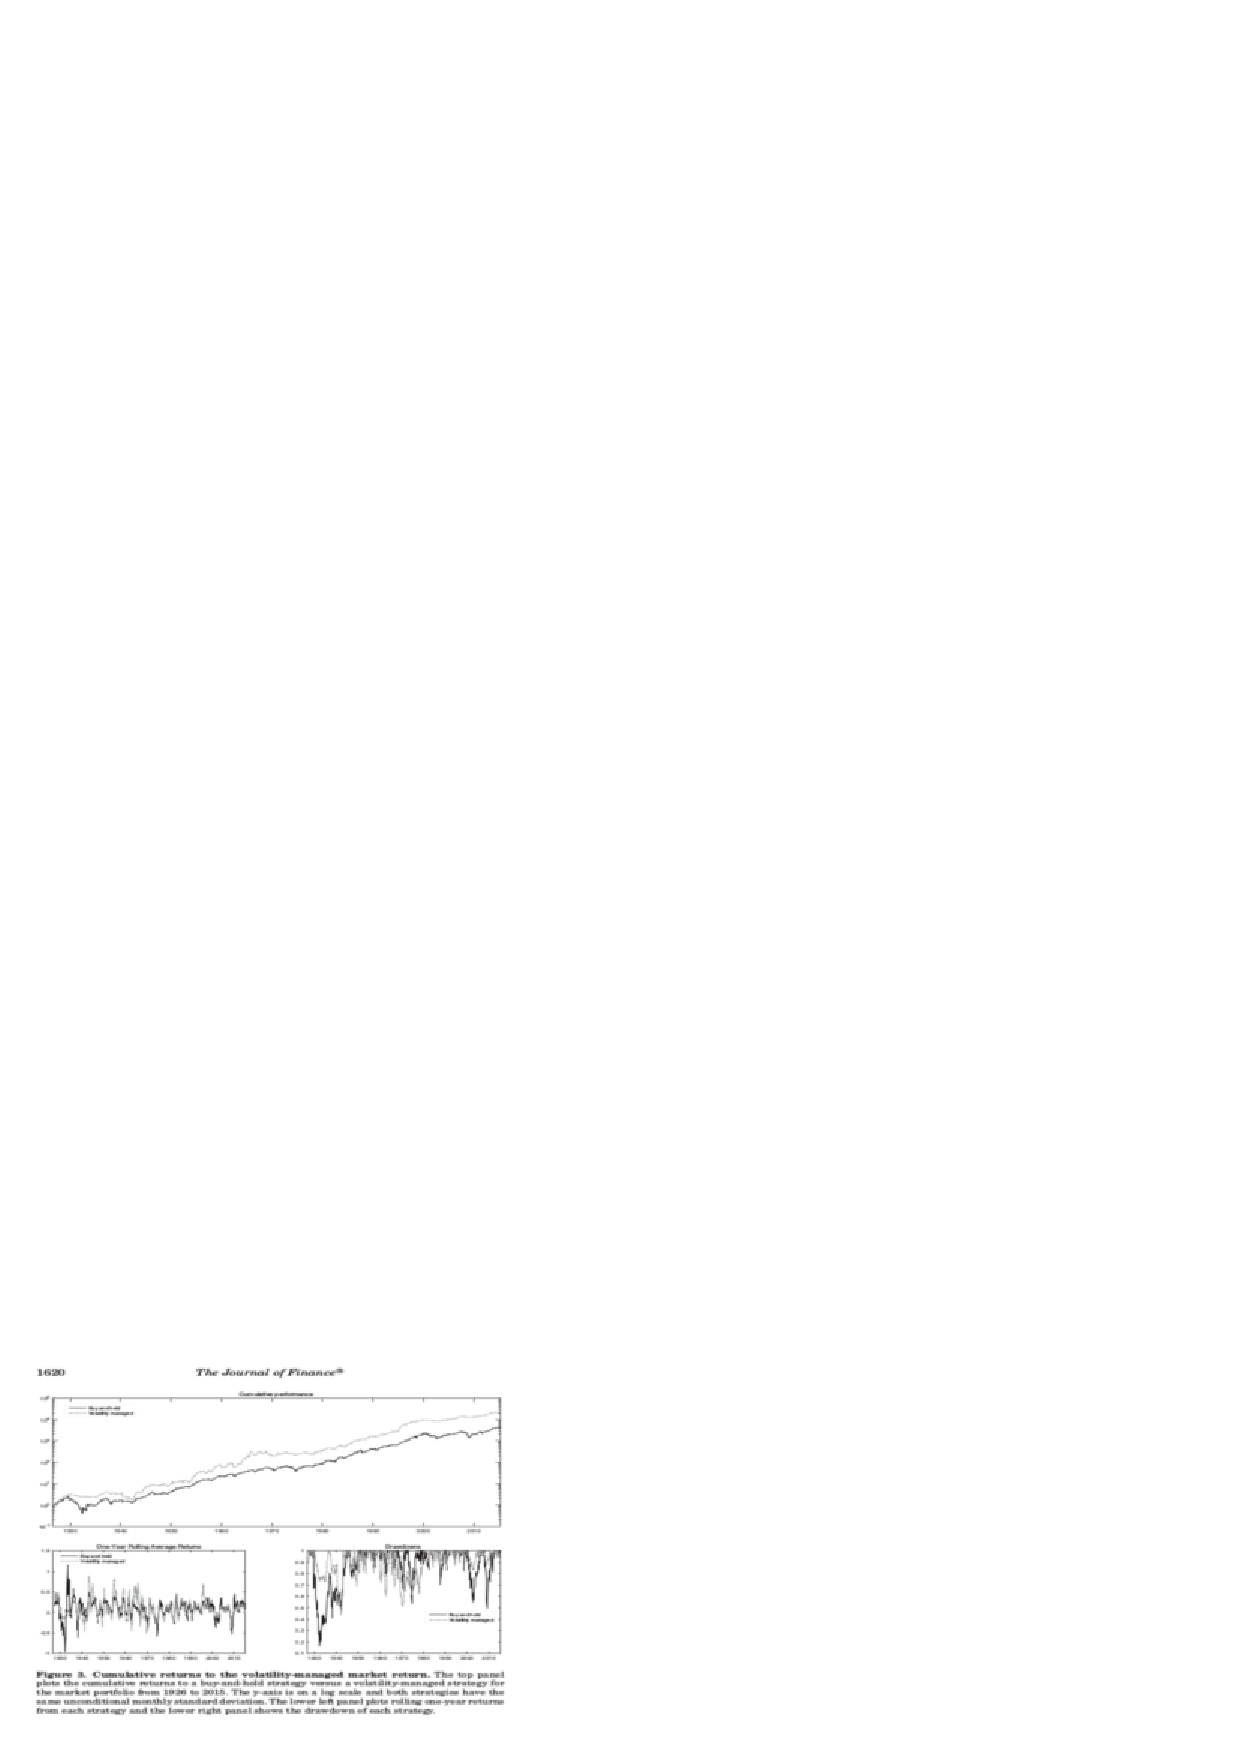
\includegraphics{mm}
%	\end{figure}
%
%\end{frame}

%\begin{frame}{Variance Decomposition}
%	\begin{itemize}[<+->]
%	\item[]	%\begin{block}{Market Variance}
%	Market Variance
%			\begin{itemize}[<+->]
%				\item Campbell, Lettau, and Xu (2001) - variance of individual assets vs market variance and CAPM
%				\item Pollet and Wilson (2010) - decompose quarterly variance of market portfolio - Avg cor and Avg var
%			\end{itemize}
%	%	\end{block}
%	\item[] Avg Var and Avg Cor
%	%	\begin{block}{Avg Var and Avg Cor}
%
%			\begin{align*}
%			R_{s,t} &= \sum_{1}^{N}w_{n,t}R_{n,t} \\
%			\sigma^{2}(r_{s,t}) &= \sum_{n=1}^{N} \sum_{m=1}^{N}w_{n,t}w_{m,t}\sigma^{2}_{n,t}\sigma^{2}_{m,t}\rho_{n,m,t}\\
%			\sigma^{2}_{s,t} &= \sum_{n=1}^{N} w_{n,t}\sigma^{2}_{n,t} \times \sum_{n=1}^{N}\sum_{m \neq n}^{N}w_{n,t}w_{m,t}\rho_{n,m,t}\\
%			AV_{t} &= \sum_{n=1}^{N} w_{n,t}\sigma^{2}_{n,t} ~ \text{ and } ~ AC_{t} = \sum_{n=1}^{N}\sum_{m \neq n}^{N}w_{n,t}w_{m,t}\rho_{n,m,t}
%			\end{align*}
%	%	\end{block}
%	\end{itemize}
%	
%\end{frame}

%\begin{frame}{Pollet and Wilson 2010 - Risk}
%		\vspace{-12pt}
%		\begin{table}
%			\caption{1963Q2:2007Q1}
%			\vspace{-18pt}
%			\begin{adjustbox}{width=\textwidth,height=3cm}
%				
% Table created by stargazer v.5.2 by Marek Hlavac, Harvard University. E-mail: hlavac at fas.harvard.edu
% Date and time: Mon, Mar 26, 2018 - 03:21:07  IST
\begin{tabular}{@{\extracolsep{5pt}}lccccc} 
\\[-1.8ex]\hline 
\hline \\[-1.8ex] 
\\[-1.8ex] & \multicolumn{5}{c}{SV$_{t+1}$} \\ 
\hline \\[-1.8ex] 
 AC$_{t}$ & 0.014$^{***}$ &  & 0.005 &  &  \\ 
 & (0.005) &  & (0.005) &  &  \\ 
 & & & & & \\ 
 AV$_{t}$ &  & 0.144$^{***}$ & 0.136$^{***}$ &  & 0.188$^{***}$ \\ 
 &  & (0.023) & (0.024) &  & (0.042) \\ 
 & & & & & \\ 
 SV$_{t}$ &  &  &  & 0.310$^{***}$ & $-$0.156 \\ 
 &  &  &  & (0.072) & (0.124) \\ 
 & & & & & \\ 
 Constant & 0.002 & 0.002$^{**}$ & 0.001 & 0.003$^{***}$ & 0.001$^{**}$ \\ 
 & (0.001) & (0.001) & (0.001) & (0.001) & (0.001) \\ 
 & & & & & \\ 
\hline \\[-1.8ex] 
Observations & 176 & 176 & 176 & 176 & 176 \\ 
R$^{2}$ & 0.042 & 0.184 & 0.096 & 0.096 & 0.191 \\ 
Adjusted R$^{2}$ & 0.037 & 0.179 & 0.091 & 0.091 & 0.182 \\ 
%Residual Std. Error & 0.006 (df = 174) & 0.006 (df = 174) & 0.006 (df = 174) & 0.006 (df = 174) & 0.006 (df = 173) \\ 
%F Statistic & 7.643$^{***}$ (df = 1; 174) & 39.124$^{***}$ (df = 1; 174) & 18.577$^{***}$ (df = 1; 174) & 18.577$^{***}$ (df = 1; 174) & 20.412$^{***}$ (df = 2; 173) \\ 
\hline 
\hline \\[-1.8ex] 
\textit{Note:}  & \multicolumn{5}{r}{$^{*}$p$<$0.1; $^{**}$p$<$0.05; $^{***}$p$<$0.01} \\ 
\end{tabular} 

%			\end{adjustbox}
%		\end{table}
%\end{frame}
%
%\begin{frame}{Pollet and Wilson 2010 - Returns}
%		\vspace{-12pt}
%		\begin{table}
%			\caption{1963Q2:2007Q1}
%			\vspace{-18pt}
%			\begin{adjustbox}{width=\textwidth,height=3cm}
%				
% Table created by stargazer v.5.2 by Marek Hlavac, Harvard University. E-mail: hlavac at fas.harvard.edu
% Date and time: Tue, Mar 13, 2018 - 07:14:38  IST
\begin{table}[!htbp] \centering 
  \caption{} 
  \label{} 
\begin{tabular}{@{\extracolsep{5pt}}lcccc} 
\\[-1.8ex]\hline 
\hline \\[-1.8ex] 
 & \multicolumn{4}{c}{\textit{Dependent variable:}} \\ 
\cline{2-5} 
\\[-1.8ex] & \multicolumn{4}{c}{RET$_{t+1}} \\ 
\\[-1.8ex] & (1) & (2) & (3) & (4)\\ 
\hline \\[-1.8ex] 
 AC$_{t}$ & 0.213$^{***}$ &  &  &  \\ 
  & (0.069) &  &  &  \\ 
  & & & & \\ 
 AV$_{t}$ &  & $-$0.117 &  & $-$1.742$^{***}$ \\ 
  &  & (0.347) &  & (0.616) \\ 
  & & & & \\ 
 SV$_{t}$ &  &  & 1.454 & 5.778$^{***}$ \\ 
  &  &  & (1.025) & (1.829) \\ 
  & & & & \\ 
 Constant & $-$0.037$^{**}$ & 0.014 & 0.005 & 0.022$^{**}$ \\ 
  & (0.017) & (0.010) & (0.008) & (0.010) \\ 
  & & & & \\ 
\hline \\[-1.8ex] 
Observations & 176 & 176 & 176 & 176 \\ 
R$^{2}$ & 0.053 & 0.001 & 0.011 & 0.055 \\ 
Adjusted R$^{2}$ & 0.047 & $-$0.005 & 0.006 & 0.044 \\ 
Residual Std. Error & 0.082 (df = 174) & 0.084 (df = 174) & 0.083 (df = 174) & 0.082 (df = 173) \\ 
F Statistic & 9.649$^{***}$ (df = 1; 174) & 0.113 (df = 1; 174) & 2.013 (df = 1; 174) & 5.049$^{***}$ (df = 2; 173) \\ 
\hline 
\hline \\[-1.8ex] 
\textit{Note:}  & \multicolumn{4}{r}{$^{*}$p$<$0.1; $^{**}$p$<$0.05; $^{***}$p$<$0.01} \\ 
\end{tabular} 
\end{table} 

%			\end{adjustbox}
%		\end{table}
%\end{frame}

%\begin{frame}{Average Variance}
%	\begin{itemize}[<+->]
%		\item The average variance of the individual assets in the market (AV) we can do better
%		\item We do better because AV is a signal of future risk but not a signal of future return
%		\item Pollet and Wilson (2010) demonstrate that breaking portfolio variance can be well approximated as the product of the average pairwise correlation (AC) of assets in the market and AV.
%		\item AC is the systematic component, related to changes in aggregate wealth, and correlated with higher returns. AV is not.
%		\item Scaling back investment when AV is high and investing more when AV is low reduces investment risk without reducing return over time.
%	\end{itemize}
%\end{frame}

%\begin{frame}{Central Ideas}
%	\begin{itemize}[<+->]
%		\item If we are going to manage variance to control/time risk what is the proper way?
%		\item We know that portfolio variance is the weighted summation of asset variances and covariance
%		\item Return to the fundamental make up of portfolio variance for the right signal
%		\item Why does the right signal better control exposure to uncompensated risk
%		\item Pollet and Wilson (2010) demonstrate that stock market portfolio variance (SV) $\approx$ the product of average pairwise correlation (AC) of assets in the market and average asset variance (AV).
%		\item AC is the systematic component, related to changes in aggregate wealth, and correlated with higher returns. AV is not.
%		\item AV is the right management signal it reduces exposure to uncompensated non-systematic risk without reducing returns
%	\end{itemize}
%\end{frame}

%\section{Data}
%
%\begin{frame}{Data}
%	\begin{block}{CRSP daily returns}
%		\begin{itemize}
%			\item NYSE daily return (1926-2017)
%			\item NYSE-AMEX daily returns (1962-2017)
%			\item NASDAQ daily returns (1974-2017)
%			\item Monthly Variance Stats and MCAP of gaming industry
%		\end{itemize}
%	\end{block}
%	\begin{block}{Asaif Manela's Website}
%		\begin{itemize}
%			\item ICRF = $\frac{MarEqt}{MarEqt + BookDbt}$ He, Kelly, Manela (2017)
%			\item LF$_{AEM}$ = $\frac{FinAsst}{FinAsst - BankDbt}$ Adrian, Etula and Muir (2014)
%			\item BC = year on year increase in bank credit Gandhi (2016)
%		\end{itemize}
%	\end{block}
%	\begin{block}{NYSE}
%		\begin{itemize}
%			\item $\Delta$ MD = month to month change in Margin Debt
%		\end{itemize}
%	\end{block}	
%\end{frame}
%
%\section{Variance Decomposition}
%
%%\begin{frame}{Market Variance}
%%	\begin{align}
%%	%SV_{t} &= \frac{1}{t-1}\sum_{\tau = 1}^{t} \left(R^{m}_{\tau} - \frac{\sum_{\tau = 1}^{t} R^{m}_{\tau}}{t}\right)^{2}\\
%%	SV_{t} &= \sum_{n=1}^{N} \sum_{m=1}^{N}w^{n}_{t}w^{m}_{t}\sigma^{2}_{n,t}\sigma^{2}_{m,t}\rho^{n,m}_{t}\\
%%	SV_{t} &= \sum_{n=1}^{N} w^{n}_{t}\sigma^{2}_{n,t} \times \sum_{n=1}^{N}\sum_{m \neq n}^{N}w^{n}_{t}w^{m}_{t}\rho^{n,m}_{t}\\
%%	AV_{t} &= \sum_{n=1}^{N} w^{n}_{t}\sigma^{2}_{n,t}\\
%%	AC_{t} &= \sum_{n=1}^{N}\sum_{m \neq n}^{N}w^{n}_{t}w^{m}_{t}\rho^{n,m}_{t}\\
%%	\end{align}
%%\end{frame}
%
%\begin{frame}{Summary Stats}
%	\begin{table}[!htbp] \centering 
%		\begin{adjustbox}{width=\textwidth}
%			\begin{tabular}{lcccccc} 
%				%
% Table created by stargazer v.5.2 by Marek Hlavac, Harvard University. E-mail: hlavac at fas.harvard.edu
% Date and time: Tue, Mar 13, 2018 - 01:43:24  IST
\begin{table}[!htbp] \centering 
  \caption{} 
  \label{} 
\begin{tabular}{@{\extracolsep{5pt}}lccccc} 
\\[-1.8ex]\hline 
\hline \\[-1.8ex] 
Statistic & \multicolumn{1}{c}{N} & \multicolumn{1}{c}{Mean} & \multicolumn{1}{c}{St. Dev.} & \multicolumn{1}{c}{Min} & \multicolumn{1}{c}{Max} \\ 
\hline \\[-1.8ex] 
RET & 176 & 1.163 & 8.369 & $-$30.072 & 19.956 \\ 
AC & 176 & 0.230 & 0.090 & 0.034 & 0.648 \\ 
AV & 176 & 2.218 & 1.828 & 0.634 & 12.044 \\ 
SV & 176 & 0.483 & 0.616 & 0.029 & 6.397 \\ 
\hline \\[-1.8ex] 
\end{tabular} 
\end{table} 

%				%
% Table created by stargazer v.5.2 by Marek Hlavac, Harvard University. E-mail: hlavac at fas.harvard.edu
% Date and time: Tue, Mar 13, 2018 - 07:14:23  IST
\begin{table}[!htbp] \centering 
  \caption{} 
  \label{} 
\begin{tabular}{@{\extracolsep{5pt}}lccccc} 
\\[-1.8ex]\hline 
\hline \\[-1.8ex] 
Statistic & \multicolumn{1}{c}{N} & \multicolumn{1}{c}{Mean} & \multicolumn{1}{c}{St. Dev.} & \multicolumn{1}{c}{Min} & \multicolumn{1}{c}{Max} \\ 
\hline \\[-1.8ex] 
RET & 331 & 1.694 & 8.591 & $-$30.072 & 30.956 \\ 
AC & 364 & 0.282 & 0.121 & 0.034 & 0.678 \\ 
AV & 364 & 2.533 & 2.839 & 0.539 & 20.485 \\ 
SV & 364 & 0.741 & 1.258 & 0.029 & 11.378 \\ 
\hline \\[-1.8ex] 
\end{tabular} 
\end{table} 

%				
% Table created by stargazer v.5.2 by Marek Hlavac, Harvard University. E-mail: hlavac at fas.harvard.edu
% Date and time: Tue, Mar 13, 2018 - 01:59:12  IST
\begin{table}[!htbp] \centering 
  \caption{} 
  \label{} 
\begin{tabular}{@{\extracolsep{5pt}}lccccc} 
\\[-1.8ex]\hline 
\hline \\[-1.8ex] 
Statistic & \multicolumn{1}{c}{N} & \multicolumn{1}{c}{Mean} & \multicolumn{1}{c}{St. Dev.} & \multicolumn{1}{c}{Min} & \multicolumn{1}{c}{Max} \\ 
\hline \\[-1.8ex] 
RET & 1,085 & 0.494 & 5.371 & $-$34.553 & 33.258 \\ 
RET3 & 1,083 & 1.482 & 9.911 & $-$55.206 & 64.968 \\ 
AC & 1,086 & 0.239 & 0.105 & 0.041 & 0.702 \\ 
AV & 1,086 & 2.432 & 2.898 & 0.502 & 33.961 \\ 
SV & 1,086 & 0.691 & 1.147 & 0.031 & 11.417 \\ 
\hline \\[-1.8ex] 
\end{tabular} 
\end{table} 

%			\end{tabular}
%		\end{adjustbox}
%	\end{table}
%\end{frame}

\section{Results}
\subsection{Performance}
%\begin{frame}{Performance}
%	\begin{adjustbox}{width=\textwidth}
%		\begin{tabular}{cccccc}
%			\multicolumn{6}{c}{1926:08-2016:12}\\
%			\hline \hline \\[-1.8ex] 
%			& Return & Sharpe & Max DD & $|\delta\omega|$ & Break Even \\ 
%			\hline \\[-1.8ex] 
%			BH & 5.932 & 0.319 & -84.8 &  &  \\ 
%			SV & 8.598 & 0.462 & -63.6 & .75 & 30.7 \\ 
%			AV & 9.677*** & 0.520* & -60.3 & .32 & 83.1\\ 
%			\hline
%		\end{tabular}
%	\end{adjustbox}
%
%\end{frame}
%\begin{frame}{US Equity Performance}
%	\only<1>{\begin{figure}
%		\resizebox{11cm}{6.5cm}{% Created by tikzDevice version 0.10.1 on 2018-08-09 00:46:14
% !TEX encoding = UTF-8 Unicode
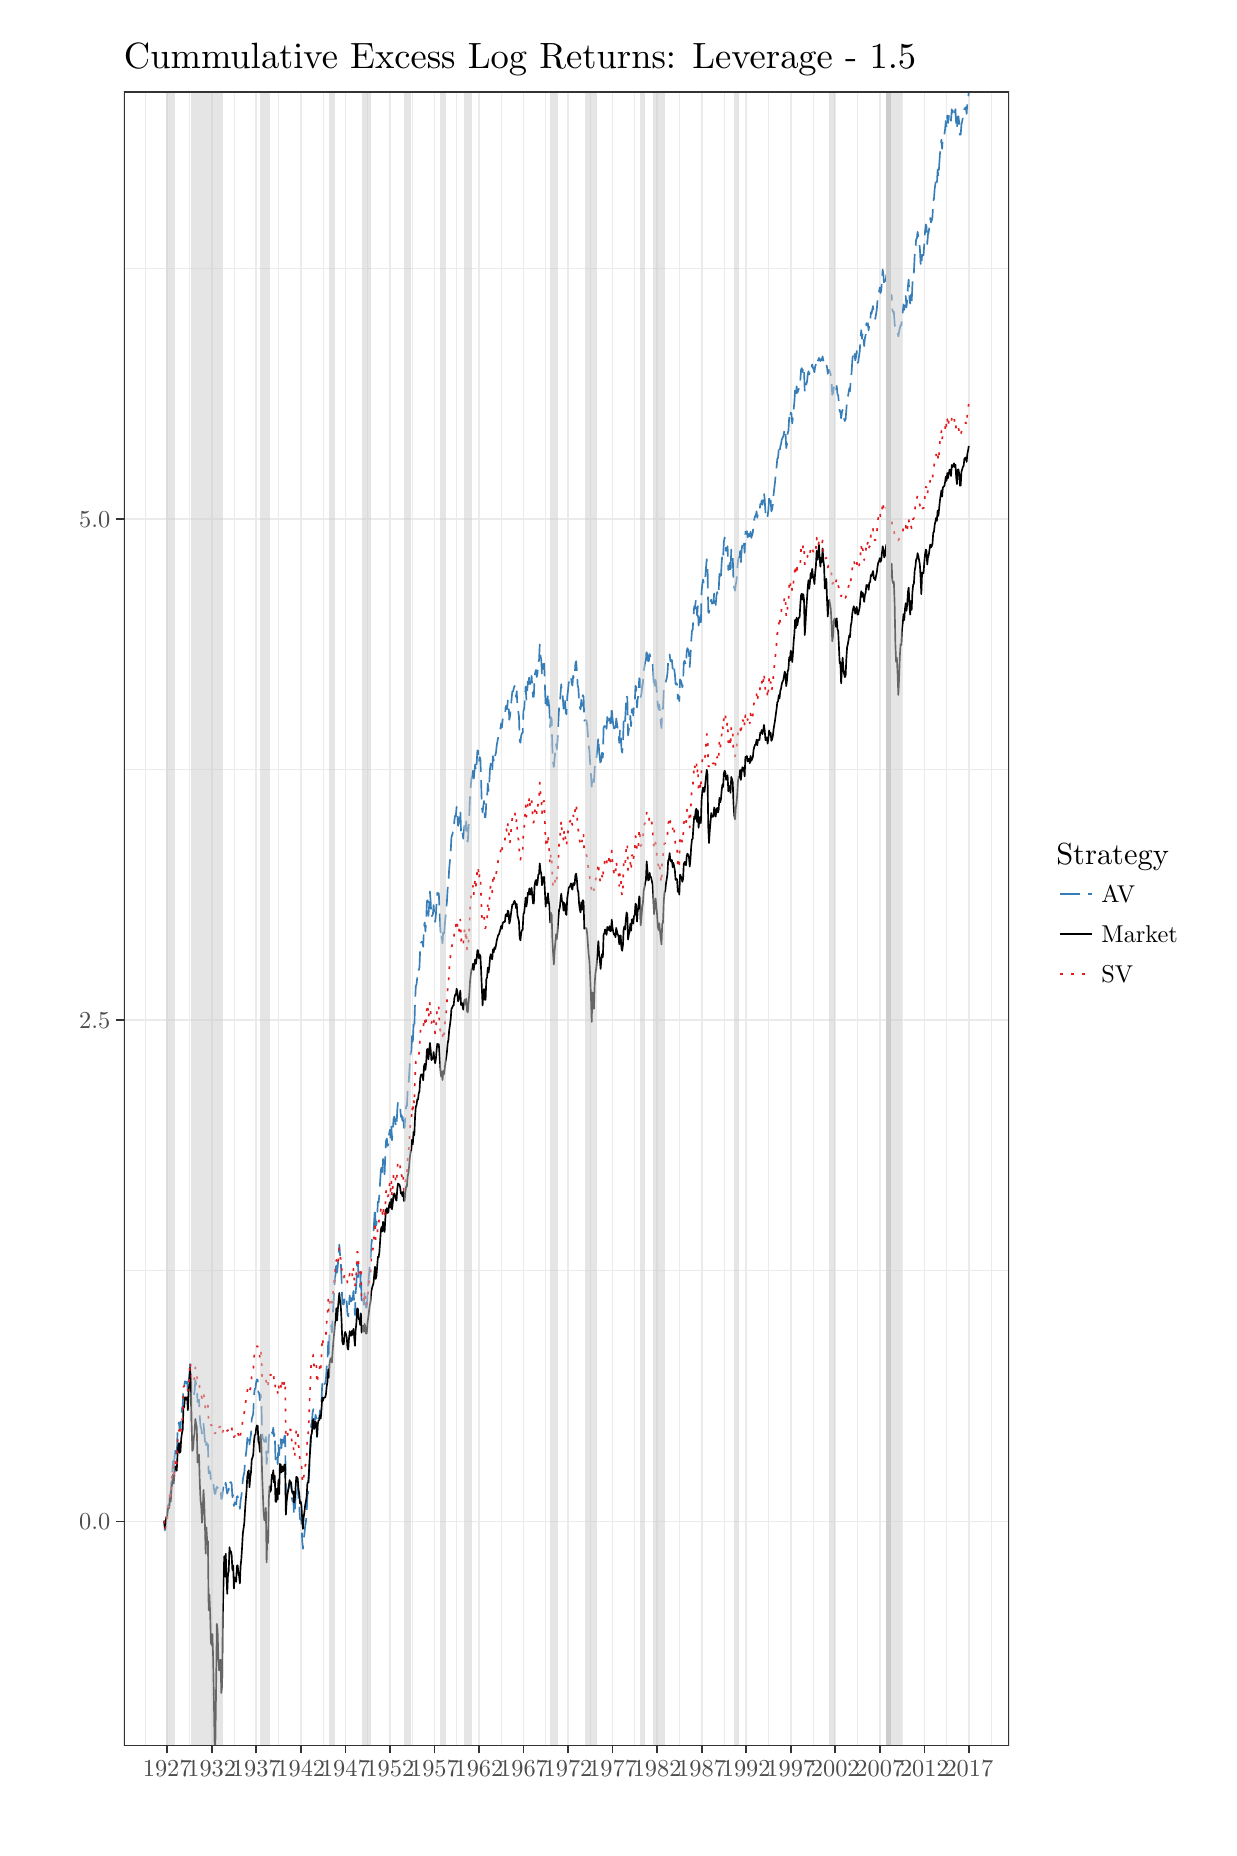
\begin{tikzpicture}[x=1pt,y=1pt]
\definecolor{fillColor}{RGB}{255,255,255}
\path[use as bounding box,fill=fillColor,fill opacity=0.00] (0,0) rectangle (426.79,650.43);
\begin{scope}
\path[clip] (  0.00,  0.00) rectangle (426.79,650.43);
\definecolor{drawColor}{RGB}{255,255,255}
\definecolor{fillColor}{RGB}{255,255,255}

\path[draw=drawColor,line width= 0.6pt,line join=round,line cap=round,fill=fillColor] (  0.00,  0.00) rectangle (426.79,650.43);
\end{scope}
\begin{scope}
\path[clip] ( 34.77, 29.59) rectangle (354.63,627.29);
\definecolor{fillColor}{RGB}{255,255,255}

\path[fill=fillColor] ( 34.77, 29.59) rectangle (354.63,627.29);
\definecolor{drawColor}{gray}{0.92}

\path[draw=drawColor,line width= 0.3pt,line join=round] ( 34.77,201.22) --
	(354.63,201.22);

\path[draw=drawColor,line width= 0.3pt,line join=round] ( 34.77,382.38) --
	(354.63,382.38);

\path[draw=drawColor,line width= 0.3pt,line join=round] ( 34.77,563.55) --
	(354.63,563.55);

\path[draw=drawColor,line width= 0.3pt,line join=round] ( 42.37, 29.59) --
	( 42.37,627.29);

\path[draw=drawColor,line width= 0.3pt,line join=round] ( 58.46, 29.59) --
	( 58.46,627.29);

\path[draw=drawColor,line width= 0.3pt,line join=round] ( 74.56, 29.59) --
	( 74.56,627.29);

\path[draw=drawColor,line width= 0.3pt,line join=round] ( 90.66, 29.59) --
	( 90.66,627.29);

\path[draw=drawColor,line width= 0.3pt,line join=round] (106.75, 29.59) --
	(106.75,627.29);

\path[draw=drawColor,line width= 0.3pt,line join=round] (122.84, 29.59) --
	(122.84,627.29);

\path[draw=drawColor,line width= 0.3pt,line join=round] (138.94, 29.59) --
	(138.94,627.29);

\path[draw=drawColor,line width= 0.3pt,line join=round] (155.04, 29.59) --
	(155.04,627.29);

\path[draw=drawColor,line width= 0.3pt,line join=round] (171.13, 29.59) --
	(171.13,627.29);

\path[draw=drawColor,line width= 0.3pt,line join=round] (187.22, 29.59) --
	(187.22,627.29);

\path[draw=drawColor,line width= 0.3pt,line join=round] (203.32, 29.59) --
	(203.32,627.29);

\path[draw=drawColor,line width= 0.3pt,line join=round] (219.41, 29.59) --
	(219.41,627.29);

\path[draw=drawColor,line width= 0.3pt,line join=round] (235.51, 29.59) --
	(235.51,627.29);

\path[draw=drawColor,line width= 0.3pt,line join=round] (251.60, 29.59) --
	(251.60,627.29);

\path[draw=drawColor,line width= 0.3pt,line join=round] (267.70, 29.59) --
	(267.70,627.29);

\path[draw=drawColor,line width= 0.3pt,line join=round] (283.79, 29.59) --
	(283.79,627.29);

\path[draw=drawColor,line width= 0.3pt,line join=round] (299.88, 29.59) --
	(299.88,627.29);

\path[draw=drawColor,line width= 0.3pt,line join=round] (315.98, 29.59) --
	(315.98,627.29);

\path[draw=drawColor,line width= 0.3pt,line join=round] (332.07, 29.59) --
	(332.07,627.29);

\path[draw=drawColor,line width= 0.3pt,line join=round] (348.17, 29.59) --
	(348.17,627.29);

\path[draw=drawColor,line width= 0.6pt,line join=round] ( 34.77,110.64) --
	(354.63,110.64);

\path[draw=drawColor,line width= 0.6pt,line join=round] ( 34.77,291.80) --
	(354.63,291.80);

\path[draw=drawColor,line width= 0.6pt,line join=round] ( 34.77,472.97) --
	(354.63,472.97);

\path[draw=drawColor,line width= 0.6pt,line join=round] ( 50.42, 29.59) --
	( 50.42,627.29);

\path[draw=drawColor,line width= 0.6pt,line join=round] ( 66.51, 29.59) --
	( 66.51,627.29);

\path[draw=drawColor,line width= 0.6pt,line join=round] ( 82.61, 29.59) --
	( 82.61,627.29);

\path[draw=drawColor,line width= 0.6pt,line join=round] ( 98.70, 29.59) --
	( 98.70,627.29);

\path[draw=drawColor,line width= 0.6pt,line join=round] (114.80, 29.59) --
	(114.80,627.29);

\path[draw=drawColor,line width= 0.6pt,line join=round] (130.89, 29.59) --
	(130.89,627.29);

\path[draw=drawColor,line width= 0.6pt,line join=round] (146.99, 29.59) --
	(146.99,627.29);

\path[draw=drawColor,line width= 0.6pt,line join=round] (163.08, 29.59) --
	(163.08,627.29);

\path[draw=drawColor,line width= 0.6pt,line join=round] (179.17, 29.59) --
	(179.17,627.29);

\path[draw=drawColor,line width= 0.6pt,line join=round] (195.27, 29.59) --
	(195.27,627.29);

\path[draw=drawColor,line width= 0.6pt,line join=round] (211.37, 29.59) --
	(211.37,627.29);

\path[draw=drawColor,line width= 0.6pt,line join=round] (227.46, 29.59) --
	(227.46,627.29);

\path[draw=drawColor,line width= 0.6pt,line join=round] (243.55, 29.59) --
	(243.55,627.29);

\path[draw=drawColor,line width= 0.6pt,line join=round] (259.64, 29.59) --
	(259.64,627.29);

\path[draw=drawColor,line width= 0.6pt,line join=round] (275.75, 29.59) --
	(275.75,627.29);

\path[draw=drawColor,line width= 0.6pt,line join=round] (291.84, 29.59) --
	(291.84,627.29);

\path[draw=drawColor,line width= 0.6pt,line join=round] (307.93, 29.59) --
	(307.93,627.29);

\path[draw=drawColor,line width= 0.6pt,line join=round] (324.02, 29.59) --
	(324.02,627.29);

\path[draw=drawColor,line width= 0.6pt,line join=round] (340.12, 29.59) --
	(340.12,627.29);
\definecolor{drawColor}{RGB}{55,126,184}

\path[draw=drawColor,line width= 0.6pt,dash pattern=on 7pt off 3pt ,line join=round] ( 49.31,110.92) --
	( 49.58,107.45) --
	( 49.84,109.26) --
	( 50.12,112.05) --
	( 50.38,111.97) --
	( 50.66,116.49) --
	( 50.93,116.63) --
	( 51.18,117.02) --
	( 51.45,122.42) --
	( 51.71,119.97) --
	( 51.99,126.59) --
	( 52.25,128.64) --
	( 52.52,132.48) --
	( 52.80,128.54) --
	( 53.06,134.22) --
	( 53.33,136.23) --
	( 53.60,135.71) --
	( 53.87,133.96) --
	( 54.15,143.10) --
	( 54.40,145.56) --
	( 54.67,146.46) --
	( 54.94,143.64) --
	( 55.21,143.91) --
	( 55.48,149.26) --
	( 55.75,151.30) --
	( 56.02,152.48) --
	( 56.29,159.57) --
	( 56.56,159.64) --
	( 56.82,161.26) --
	( 57.10,161.21) --
	( 57.37,160.59) --
	( 57.62,161.14) --
	( 57.89,157.65) --
	( 58.16,161.60) --
	( 58.43,163.63) --
	( 58.69,167.54) --
	( 58.97,165.37) --
	( 59.24,155.96) --
	( 59.50,155.38) --
	( 59.78,155.47) --
	( 60.04,156.48) --
	( 60.31,157.59) --
	( 60.59,161.69) --
	( 60.83,160.52) --
	( 61.11,159.59) --
	( 61.37,153.83) --
	( 61.64,154.58) --
	( 61.91,154.61) --
	( 62.18,148.61) --
	( 62.46,144.91) --
	( 62.72,144.36) --
	( 62.99,142.37) --
	( 63.26,143.58) --
	( 63.53,145.92) --
	( 63.80,142.86) --
	( 64.05,139.75) --
	( 64.32,137.14) --
	( 64.59,139.23) --
	( 64.86,138.44) --
	( 65.13,138.51) --
	( 65.40,128.05) --
	( 65.67,128.95) --
	( 65.94,128.39) --
	( 66.21,125.89) --
	( 66.47,125.79) --
	( 66.75,126.35) --
	( 67.02,125.18) --
	( 67.28,122.86) --
	( 67.55,120.70) --
	( 67.81,120.65) --
	( 68.09,122.35) --
	( 68.35,123.11) --
	( 68.62,122.94) --
	( 68.90,122.42) --
	( 69.16,122.09) --
	( 69.44,122.59) --
	( 69.70,122.70) --
	( 69.97,118.74) --
	( 70.25,119.29) --
	( 70.49,121.64) --
	( 70.77,123.33) --
	( 71.03,124.89) --
	( 71.30,123.77) --
	( 71.57,124.66) --
	( 71.84,122.34) --
	( 72.11,120.70) --
	( 72.38,121.76) --
	( 72.65,122.14) --
	( 72.92,125.39) --
	( 73.19,124.72) --
	( 73.46,124.85) --
	( 73.71,124.17) --
	( 73.98,119.40) --
	( 74.25,120.14) --
	( 74.52,116.23) --
	( 74.78,117.50) --
	( 75.06,117.43) --
	( 75.33,116.72) --
	( 75.60,119.60) --
	( 75.87,119.77) --
	( 76.13,118.30) --
	( 76.41,117.19) --
	( 76.68,115.22) --
	( 76.93,118.23) --
	( 77.20,119.70) --
	( 77.46,122.00) --
	( 77.74,125.61) --
	( 78.00,127.21) --
	( 78.27,128.19) --
	( 78.55,132.44) --
	( 78.81,134.45) --
	( 79.09,136.71) --
	( 79.35,140.32) --
	( 79.62,141.67) --
	( 79.90,142.17) --
	( 80.15,138.45) --
	( 80.43,140.67) --
	( 80.69,142.10) --
	( 80.96,147.71) --
	( 81.23,148.56) --
	( 81.50,149.45) --
	( 81.77,156.07) --
	( 82.04,158.50) --
	( 82.31,158.64) --
	( 82.58,161.03) --
	( 82.85,161.98) --
	( 83.12,161.74) --
	( 83.37,157.30) --
	( 83.64,156.99) --
	( 83.91,154.44) --
	( 84.18,156.56) --
	( 84.44,154.00) --
	( 84.72,142.41) --
	( 84.99,140.63) --
	( 85.25,139.94) --
	( 85.53,139.46) --
	( 85.79,139.67) --
	( 86.07,141.21) --
	( 86.34,131.42) --
	( 86.59,134.55) --
	( 86.86,133.86) --
	( 87.12,140.77) --
	( 87.40,142.58) --
	( 87.66,141.65) --
	( 87.93,141.78) --
	( 88.21,143.10) --
	( 88.47,142.33) --
	( 88.74,144.48) --
	( 89.01,141.42) --
	( 89.28,142.63) --
	( 89.56,133.04) --
	( 89.80,132.96) --
	( 90.08,134.86) --
	( 90.34,131.34) --
	( 90.61,138.64) --
	( 90.88,134.52) --
	( 91.15,140.43) --
	( 91.42,140.38) --
	( 91.69,137.14) --
	( 91.96,140.32) --
	( 92.23,137.90) --
	( 92.50,139.47) --
	( 92.77,141.48) --
	( 93.03,141.57) --
	( 93.30,117.95) --
	( 93.57,118.87) --
	( 93.84,119.68) --
	( 94.10,121.76) --
	( 94.38,123.12) --
	( 94.65,124.93) --
	( 94.91,123.51) --
	( 95.19,123.79) --
	( 95.45,119.21) --
	( 95.72,117.92) --
	( 96.00,118.65) --
	( 96.24,113.01) --
	( 96.52,114.06) --
	( 96.78,119.11) --
	( 97.06,125.40) --
	( 97.32,125.29) --
	( 97.59,124.43) --
	( 97.87,118.51) --
	( 98.13,116.42) --
	( 98.40,111.51) --
	( 98.67,111.76) --
	( 98.94,110.37) --
	( 99.21,103.55) --
	( 99.46,100.77) --
	( 99.73,104.26) --
	(100.00,106.08) --
	(100.27,108.92) --
	(100.54,110.45) --
	(100.81,113.32) --
	(101.08,120.55) --
	(101.35,120.62) --
	(101.62,126.02) --
	(101.88,132.71) --
	(102.16,139.06) --
	(102.43,145.54) --
	(102.68,146.14) --
	(102.95,149.80) --
	(103.22,151.21) --
	(103.49,145.86) --
	(103.75,146.92) --
	(104.03,149.18) --
	(104.30,147.88) --
	(104.56,141.14) --
	(104.84,146.06) --
	(105.10,147.89) --
	(105.37,148.23) --
	(105.65,150.86) --
	(105.90,149.02) --
	(106.18,154.40) --
	(106.44,160.37) --
	(106.71,158.68) --
	(106.98,160.33) --
	(107.25,160.34) --
	(107.52,160.54) --
	(107.79,162.32) --
	(108.06,166.66) --
	(108.33,168.80) --
	(108.60,175.57) --
	(108.87,171.20) --
	(109.12,178.93) --
	(109.39,180.87) --
	(109.66,181.34) --
	(109.93,178.89) --
	(110.20,184.86) --
	(110.47,189.01) --
	(110.74,193.11) --
	(111.01,198.80) --
	(111.28,199.88) --
	(111.54,204.76) --
	(111.82,200.63) --
	(112.09,203.39) --
	(112.34,206.88) --
	(112.61,210.70) --
	(112.87,207.01) --
	(113.15,204.37) --
	(113.41,198.62) --
	(113.69,189.38) --
	(113.96,189.09) --
	(114.22,189.11) --
	(114.50,191.67) --
	(114.76,192.27) --
	(115.03,191.40) --
	(115.31,189.56) --
	(115.55,185.56) --
	(115.83,184.74) --
	(116.09,188.56) --
	(116.36,192.30) --
	(116.63,190.71) --
	(116.90,190.17) --
	(117.18,192.81) --
	(117.44,190.68) --
	(117.71,193.91) --
	(117.98,189.93) --
	(118.25,185.23) --
	(118.52,193.38) --
	(118.78,196.52) --
	(119.05,204.21) --
	(119.32,204.11) --
	(119.59,198.41) --
	(119.85,198.66) --
	(120.13,195.28) --
	(120.40,200.74) --
	(120.67,190.19) --
	(120.94,191.81) --
	(121.20,192.10) --
	(121.48,188.87) --
	(121.75,193.19) --
	(122.00,191.12) --
	(122.27,187.87) --
	(122.53,188.01) --
	(122.81,193.76) --
	(123.07,196.53) --
	(123.34,199.87) --
	(123.62,203.17) --
	(123.88,205.07) --
	(124.15,210.51) --
	(124.42,212.34) --
	(124.69,213.89) --
	(124.97,215.16) --
	(125.21,219.40) --
	(125.49,223.99) --
	(125.75,217.40) --
	(126.02,218.13) --
	(126.29,221.09) --
	(126.56,226.19) --
	(126.83,225.95) --
	(127.10,228.95) --
	(127.37,233.59) --
	(127.64,237.67) --
	(127.91,238.90) --
	(128.18,236.44) --
	(128.43,241.64) --
	(128.70,239.06) --
	(128.97,236.10) --
	(129.24,243.49) --
	(129.50,248.15) --
	(129.78,248.99) --
	(130.05,246.36) --
	(130.32,246.85) --
	(130.59,250.45) --
	(130.85,252.16) --
	(131.13,249.26) --
	(131.40,253.97) --
	(131.65,248.36) --
	(131.93,251.76) --
	(132.19,255.85) --
	(132.47,256.94) --
	(132.73,256.04) --
	(133.00,253.78) --
	(133.28,253.03) --
	(133.54,259.13) --
	(133.81,262.30) --
	(134.08,262.01) --
	(134.35,261.64) --
	(134.62,260.06) --
	(134.87,256.85) --
	(135.14,257.41) --
	(135.41,255.44) --
	(135.68,257.95) --
	(135.95,252.86) --
	(136.22,253.02) --
	(136.49,257.88) --
	(136.76,260.77) --
	(137.03,260.70) --
	(137.30,266.20) --
	(137.57,267.95) --
	(137.84,271.82) --
	(138.09,276.33) --
	(138.36,279.64) --
	(138.63,280.79) --
	(138.90,286.11) --
	(139.16,283.54) --
	(139.44,290.29) --
	(139.71,288.46) --
	(139.97,298.27) --
	(140.25,304.06) --
	(140.51,304.74) --
	(140.78,307.31) --
	(141.06,307.12) --
	(141.30,309.72) --
	(141.58,310.91) --
	(141.84,317.76) --
	(142.12,319.79) --
	(142.38,320.10) --
	(142.65,319.77) --
	(142.93,318.29) --
	(143.19,325.51) --
	(143.46,327.09) --
	(143.73,323.81) --
	(144.00,327.83) --
	(144.27,334.79) --
	(144.53,335.14) --
	(144.80,329.48) --
	(145.07,333.14) --
	(145.34,338.28) --
	(145.61,334.77) --
	(145.88,329.00) --
	(146.15,329.61) --
	(146.42,329.92) --
	(146.69,333.38) --
	(146.95,329.62) --
	(147.23,327.30) --
	(147.50,329.60) --
	(147.75,334.14) --
	(148.02,337.81) --
	(148.28,336.99) --
	(148.56,337.67) --
	(148.82,331.83) --
	(149.10,325.73) --
	(149.37,320.88) --
	(149.63,321.93) --
	(149.91,319.55) --
	(150.17,324.50) --
	(150.44,322.68) --
	(150.72,325.98) --
	(150.96,329.15) --
	(151.24,331.69) --
	(151.50,334.77) --
	(151.77,339.41) --
	(152.04,341.45) --
	(152.31,346.54) --
	(152.59,349.41) --
	(152.85,352.48) --
	(153.12,357.91) --
	(153.39,358.73) --
	(153.66,359.70) --
	(153.93,359.98) --
	(154.18,363.82) --
	(154.45,365.69) --
	(154.72,365.54) --
	(154.99,368.88) --
	(155.26,367.25) --
	(155.53,361.97) --
	(155.80,363.32) --
	(156.07,364.98) --
	(156.34,367.66) --
	(156.60,359.93) --
	(156.88,361.12) --
	(157.15,359.35) --
	(157.41,357.37) --
	(157.68,360.63) --
	(157.94,362.84) --
	(158.22,360.44) --
	(158.48,363.63) --
	(158.75,356.91) --
	(159.03,356.31) --
	(159.29,360.96) --
	(159.57,365.87) --
	(159.83,372.47) --
	(160.10,376.24) --
	(160.38,379.32) --
	(160.62,379.78) --
	(160.90,381.88) --
	(161.16,378.56) --
	(161.43,381.57) --
	(161.70,384.23) --
	(161.97,381.84) --
	(162.24,384.62) --
	(162.51,389.27) --
	(162.78,389.14) --
	(163.05,384.97) --
	(163.32,386.87) --
	(163.59,386.10) --
	(163.84,378.76) --
	(164.11,368.93) --
	(164.38,366.87) --
	(164.65,369.18) --
	(164.91,370.98) --
	(165.19,365.09) --
	(165.46,365.08) --
	(165.73,370.99) --
	(166.00,372.00) --
	(166.26,377.28) --
	(166.54,374.62) --
	(166.81,377.87) --
	(167.06,382.66) --
	(167.33,384.56) --
	(167.59,382.31) --
	(167.87,381.87) --
	(168.13,387.20) --
	(168.40,385.60) --
	(168.68,388.30) --
	(168.94,387.41) --
	(169.22,388.51) --
	(169.48,390.99) --
	(169.75,392.53) --
	(170.03,394.10) --
	(170.28,394.32) --
	(170.55,395.86) --
	(170.82,397.17) --
	(171.09,399.05) --
	(171.36,397.50) --
	(171.63,400.43) --
	(171.90,401.09) --
	(172.17,401.12) --
	(172.44,401.21) --
	(172.71,405.01) --
	(172.98,405.43) --
	(173.25,404.06) --
	(173.50,407.34) --
	(173.77,406.47) --
	(174.04,400.35) --
	(174.31,401.74) --
	(174.57,404.67) --
	(174.85,407.75) --
	(175.12,410.53) --
	(175.38,410.53) --
	(175.66,411.65) --
	(175.92,412.58) --
	(176.20,411.28) --
	(176.47,408.57) --
	(176.72,410.64) --
	(176.99,404.36) --
	(177.25,403.42) --
	(177.53,401.57) --
	(177.79,392.63) --
	(178.06,392.05) --
	(178.34,394.74) --
	(178.60,395.45) --
	(178.87,395.62) --
	(179.14,403.62) --
	(179.41,404.28) --
	(179.69,408.43) --
	(179.93,412.35) --
	(180.21,407.57) --
	(180.47,410.05) --
	(180.74,414.19) --
	(181.01,413.25) --
	(181.28,416.58) --
	(181.55,413.22) --
	(181.82,413.73) --
	(182.09,416.22) --
	(182.36,411.81) --
	(182.63,408.59) --
	(182.90,408.70) --
	(183.16,415.95) --
	(183.43,417.60) --
	(183.70,418.33) --
	(183.97,415.81) --
	(184.23,417.08) --
	(184.51,421.28) --
	(184.78,421.81) --
	(185.04,427.52) --
	(185.32,423.30) --
	(185.58,422.11) --
	(185.85,416.14) --
	(186.13,418.83) --
	(186.37,420.54) --
	(186.65,420.59) --
	(186.91,412.43) --
	(187.18,405.06) --
	(187.45,407.94) --
	(187.72,405.42) --
	(188.00,409.87) --
	(188.26,406.81) --
	(188.53,404.00) --
	(188.80,397.66) --
	(189.07,401.30) --
	(189.34,400.56) --
	(189.59,390.07) --
	(189.86,384.77) --
	(190.13,383.27) --
	(190.40,386.45) --
	(190.67,388.82) --
	(190.94,391.46) --
	(191.21,389.65) --
	(191.48,393.49) --
	(191.75,399.29) --
	(192.01,404.31) --
	(192.29,405.64) --
	(192.56,409.99) --
	(192.81,413.20) --
	(193.08,408.84) --
	(193.35,408.87) --
	(193.62,404.31) --
	(193.88,408.44) --
	(194.16,407.88) --
	(194.43,402.86) --
	(194.69,402.32) --
	(194.97,408.65) --
	(195.23,410.76) --
	(195.50,413.71) --
	(195.78,414.34) --
	(196.03,414.67) --
	(196.31,416.14) --
	(196.57,413.53) --
	(196.84,412.74) --
	(197.11,416.27) --
	(197.38,415.26) --
	(197.65,415.88) --
	(197.92,420.71) --
	(198.19,421.49) --
	(198.46,418.06) --
	(198.73,412.85) --
	(199.00,411.78) --
	(199.25,407.16) --
	(199.52,404.85) --
	(199.79,404.10) --
	(200.06,407.56) --
	(200.33,405.30) --
	(200.60,409.24) --
	(200.87,408.68) --
	(201.14,399.99) --
	(201.41,400.20) --
	(201.67,400.17) --
	(201.95,400.01) --
	(202.22,397.97) --
	(202.47,394.18) --
	(202.74,390.70) --
	(203.00,389.06) --
	(203.28,384.01) --
	(203.54,380.54) --
	(203.81,376.16) --
	(204.09,380.13) --
	(204.35,379.14) --
	(204.63,377.84) --
	(204.89,383.05) --
	(205.16,384.77) --
	(205.44,386.02) --
	(205.68,388.36) --
	(205.96,391.14) --
	(206.22,394.08) --
	(206.49,388.83) --
	(206.76,386.38) --
	(207.03,383.42) --
	(207.30,386.71) --
	(207.57,388.42) --
	(207.84,386.61) --
	(208.11,397.57) --
	(208.38,397.76) --
	(208.65,399.70) --
	(208.91,398.50) --
	(209.18,397.04) --
	(209.45,401.32) --
	(209.72,400.25) --
	(209.98,399.62) --
	(210.26,401.74) --
	(210.53,399.05) --
	(210.79,399.15) --
	(211.07,405.21) --
	(211.33,400.75) --
	(211.61,398.59) --
	(211.88,397.19) --
	(212.13,397.34) --
	(212.40,395.75) --
	(212.66,400.79) --
	(212.94,398.98) --
	(213.20,397.09) --
	(213.47,396.80) --
	(213.75,391.97) --
	(214.01,396.33) --
	(214.28,396.69) --
	(214.55,389.98) --
	(214.82,388.44) --
	(215.10,391.54) --
	(215.34,399.69) --
	(215.62,401.55) --
	(215.88,399.83) --
	(216.15,405.28) --
	(216.42,409.20) --
	(216.69,408.04) --
	(216.96,394.65) --
	(217.23,396.91) --
	(217.50,397.61) --
	(217.77,401.78) --
	(218.04,397.98) --
	(218.31,404.06) --
	(218.56,404.19) --
	(218.83,401.83) --
	(219.10,405.94) --
	(219.37,406.67) --
	(219.63,412.61) --
	(219.91,411.93) --
	(220.18,404.74) --
	(220.44,407.91) --
	(220.72,409.49) --
	(220.98,415.33) --
	(221.26,414.95) --
	(221.53,408.51) --
	(221.78,409.82) --
	(222.06,412.02) --
	(222.32,413.68) --
	(222.60,418.15) --
	(222.86,419.41) --
	(223.13,421.19) --
	(223.41,421.85) --
	(223.67,426.27) --
	(223.94,423.75) --
	(224.21,421.49) --
	(224.48,421.65) --
	(224.75,424.09) --
	(225.00,423.00) --
	(225.27,423.09) --
	(225.54,421.66) --
	(225.81,420.95) --
	(226.08,416.29) --
	(226.35,411.45) --
	(226.62,413.42) --
	(226.89,414.77) --
	(227.16,412.64) --
	(227.42,409.21) --
	(227.70,405.58) --
	(227.97,404.22) --
	(228.22,405.86) --
	(228.49,402.95) --
	(228.76,399.35) --
	(229.03,397.36) --
	(229.29,404.17) --
	(229.57,404.38) --
	(229.84,410.94) --
	(230.10,412.34) --
	(230.38,412.67) --
	(230.64,414.30) --
	(230.91,415.30) --
	(231.19,417.13) --
	(231.43,421.14) --
	(231.71,421.66) --
	(231.97,423.95) --
	(232.25,421.58) --
	(232.51,421.36) --
	(232.78,421.96) --
	(233.06,418.82) --
	(233.32,420.39) --
	(233.59,418.81) --
	(233.86,416.88) --
	(234.13,413.16) --
	(234.40,413.51) --
	(234.66,413.18) --
	(234.93,407.88) --
	(235.20,409.18) --
	(235.47,407.09) --
	(235.74,414.91) --
	(236.01,414.48) --
	(236.28,413.65) --
	(236.55,412.08) --
	(236.82,413.54) --
	(237.08,420.84) --
	(237.36,421.69) --
	(237.63,420.80) --
	(237.88,420.01) --
	(238.15,425.24) --
	(238.41,426.22) --
	(238.69,425.47) --
	(238.95,424.45) --
	(239.23,419.36) --
	(239.50,423.49) --
	(239.76,428.65) --
	(240.04,432.53) --
	(240.30,432.84) --
	(240.57,437.35) --
	(240.85,441.36) --
	(241.09,440.37) --
	(241.37,443.01) --
	(241.63,443.81) --
	(241.90,437.94) --
	(242.17,441.39) --
	(242.44,434.38) --
	(242.72,436.56) --
	(242.98,437.43) --
	(243.25,434.82) --
	(243.52,446.63) --
	(243.79,449.44) --
	(244.06,451.00) --
	(244.31,449.46) --
	(244.58,449.48) --
	(244.85,451.77) --
	(245.12,455.45) --
	(245.39,458.37) --
	(245.66,456.38) --
	(245.93,439.35) --
	(246.20,438.94) --
	(246.47,441.01) --
	(246.73,442.35) --
	(247.01,443.74) --
	(247.28,442.25) --
	(247.54,442.69) --
	(247.81,442.42) --
	(248.07,446.31) --
	(248.35,445.27) --
	(248.61,441.80) --
	(248.88,445.22) --
	(249.16,446.48) --
	(249.42,445.11) --
	(249.69,446.72) --
	(249.96,453.06) --
	(250.23,450.57) --
	(250.51,452.29) --
	(250.75,456.74) --
	(251.03,460.21) --
	(251.29,458.96) --
	(251.56,464.58) --
	(251.83,466.19) --
	(252.10,465.37) --
	(252.37,461.34) --
	(252.64,461.82) --
	(252.91,463.05) --
	(253.18,454.42) --
	(253.45,455.03) --
	(253.72,457.01) --
	(253.97,453.27) --
	(254.24,461.84) --
	(254.51,460.63) --
	(254.78,458.94) --
	(255.04,450.45) --
	(255.32,448.23) --
	(255.59,446.98) --
	(255.86,449.15) --
	(256.13,450.58) --
	(256.39,454.27) --
	(256.67,457.74) --
	(256.94,459.08) --
	(257.19,458.98) --
	(257.46,461.33) --
	(257.72,457.25) --
	(258.00,461.72) --
	(258.26,463.83) --
	(258.53,462.58) --
	(258.81,464.00) --
	(259.07,460.65) --
	(259.35,468.29) --
	(259.61,467.95) --
	(259.88,468.49) --
	(260.16,466.21) --
	(260.41,467.35) --
	(260.68,467.54) --
	(260.95,465.16) --
	(261.22,468.30) --
	(261.49,466.07) --
	(261.76,467.08) --
	(262.03,467.95) --
	(262.30,471.18) --
	(262.57,472.84) --
	(262.84,473.93) --
	(263.11,474.16) --
	(263.38,475.66) --
	(263.63,473.35) --
	(263.90,474.83) --
	(264.17,475.11) --
	(264.44,474.85) --
	(264.70,478.30) --
	(264.98,478.13) --
	(265.25,479.61) --
	(265.51,478.02) --
	(265.79,479.42) --
	(266.05,482.51) --
	(266.32,480.00) --
	(266.60,475.17) --
	(266.84,475.77) --
	(267.12,476.19) --
	(267.38,473.87) --
	(267.66,476.33) --
	(267.92,480.48) --
	(268.19,478.49) --
	(268.47,479.65) --
	(268.73,475.61) --
	(269.00,476.47) --
	(269.27,478.13) --
	(269.54,481.78) --
	(269.81,484.22) --
	(270.06,486.34) --
	(270.33,489.30) --
	(270.60,491.57) --
	(270.87,494.61) --
	(271.14,494.96) --
	(271.41,498.15) --
	(271.68,496.60) --
	(271.95,499.11) --
	(272.22,499.90) --
	(272.49,501.63) --
	(272.76,502.21) --
	(273.03,502.72) --
	(273.29,504.00) --
	(273.56,505.63) --
	(273.82,504.53) --
	(274.10,498.50) --
	(274.36,499.91) --
	(274.64,503.93) --
	(274.91,504.86) --
	(275.17,509.53) --
	(275.45,508.12) --
	(275.71,511.35) --
	(275.98,510.99) --
	(276.26,507.42) --
	(276.50,509.59) --
	(276.78,512.48) --
	(277.04,515.07) --
	(277.31,519.72) --
	(277.58,517.55) --
	(277.85,520.85) --
	(278.13,518.46) --
	(278.39,519.16) --
	(278.66,519.94) --
	(278.93,519.97) --
	(279.20,523.18) --
	(279.47,526.91) --
	(279.72,527.37) --
	(279.99,525.98) --
	(280.26,528.02) --
	(280.53,526.54) --
	(280.80,518.66) --
	(281.07,520.17) --
	(281.34,521.50) --
	(281.61,522.51) --
	(281.88,525.12) --
	(282.14,526.28) --
	(282.42,525.12) --
	(282.69,526.26) --
	(282.94,527.72) --
	(283.21,527.21) --
	(283.47,528.70) --
	(283.75,527.56) --
	(284.01,526.90) --
	(284.29,525.92) --
	(284.56,528.00) --
	(284.82,528.77) --
	(285.10,530.86) --
	(285.36,529.91) --
	(285.63,530.26) --
	(285.91,531.10) --
	(286.16,530.36) --
	(286.44,529.95) --
	(286.70,530.69) --
	(286.97,530.28) --
	(287.24,531.62) --
	(287.51,530.01) --
	(287.78,529.29) --
	(288.05,528.11) --
	(288.32,528.37) --
	(288.59,528.81) --
	(288.86,527.60) --
	(289.13,525.38) --
	(289.38,526.67) --
	(289.65,526.76) --
	(289.92,525.94) --
	(290.19,525.01) --
	(290.45,522.85) --
	(290.73,517.74) --
	(291.00,518.31) --
	(291.27,520.28) --
	(291.54,521.03) --
	(291.80,520.07) --
	(292.08,518.98) --
	(292.35,520.99) --
	(292.60,518.15) --
	(292.87,517.60) --
	(293.13,514.88) --
	(293.41,511.78) --
	(293.67,511.87) --
	(293.94,509.24) --
	(294.22,511.40) --
	(294.48,512.34) --
	(294.76,510.47) --
	(295.02,508.96) --
	(295.29,508.29) --
	(295.57,508.94) --
	(295.81,512.23) --
	(296.09,515.82) --
	(296.35,516.84) --
	(296.62,518.48) --
	(296.89,520.13) --
	(297.16,519.06) --
	(297.43,524.06) --
	(297.70,525.37) --
	(297.97,530.13) --
	(298.24,532.53) --
	(298.51,533.77) --
	(298.78,532.53) --
	(299.04,530.20) --
	(299.31,531.34) --
	(299.58,533.57) --
	(299.85,529.33) --
	(300.11,529.52) --
	(300.39,531.62) --
	(300.66,533.42) --
	(300.92,537.50) --
	(301.20,541.14) --
	(301.46,538.05) --
	(301.74,540.32) --
	(302.01,538.28) --
	(302.26,535.34) --
	(302.53,538.28) --
	(302.79,539.30) --
	(303.07,543.65) --
	(303.33,542.75) --
	(303.60,543.64) --
	(303.88,541.02) --
	(304.14,543.57) --
	(304.41,543.66) --
	(304.68,547.59) --
	(304.95,547.15) --
	(305.23,548.82) --
	(305.47,549.85) --
	(305.75,546.02) --
	(306.01,545.69) --
	(306.28,545.23) --
	(306.55,546.88) --
	(306.82,548.53) --
	(307.09,552.04) --
	(307.36,554.14) --
	(307.63,554.87) --
	(307.90,556.50) --
	(308.17,554.54) --
	(308.44,555.46) --
	(308.69,559.29) --
	(308.96,562.98) --
	(309.23,560.88) --
	(309.50,556.93) --
	(309.76,557.51) --
	(310.04,559.03) --
	(310.31,561.21) --
	(310.57,557.83) --
	(310.85,557.58) --
	(311.11,552.82) --
	(311.39,552.04) --
	(311.66,551.47) --
	(311.91,552.87) --
	(312.19,553.83) --
	(312.45,548.39) --
	(312.72,547.62) --
	(312.99,547.80) --
	(313.26,543.62) --
	(313.54,541.66) --
	(313.80,541.25) --
	(314.07,541.40) --
	(314.34,540.41) --
	(314.61,538.87) --
	(314.88,540.57) --
	(315.13,541.70) --
	(315.40,542.93) --
	(315.67,542.85) --
	(315.94,546.31) --
	(316.21,547.67) --
	(316.48,550.37) --
	(316.75,548.44) --
	(317.02,551.08) --
	(317.29,553.47) --
	(317.55,549.39) --
	(317.83,552.08) --
	(318.10,557.23) --
	(318.35,559.39) --
	(318.62,552.63) --
	(318.89,550.71) --
	(319.16,553.93) --
	(319.42,550.96) --
	(319.70,557.64) --
	(319.97,561.41) --
	(320.23,561.93) --
	(320.51,567.99) --
	(320.77,570.04) --
	(321.04,573.94) --
	(321.32,574.29) --
	(321.56,576.64) --
	(321.84,574.99) --
	(322.10,572.98) --
	(322.38,570.93) --
	(322.64,565.53) --
	(322.91,563.97) --
	(323.19,568.36) --
	(323.45,568.15) --
	(323.72,568.29) --
	(323.99,572.46) --
	(324.26,576.76) --
	(324.53,579.33) --
	(324.79,578.59) --
	(325.06,572.27) --
	(325.33,575.85) --
	(325.60,576.56) --
	(325.87,578.80) --
	(326.14,581.64) --
	(326.41,580.09) --
	(326.68,580.75) --
	(326.95,582.01) --
	(327.21,587.72) --
	(327.49,588.61) --
	(327.76,592.38) --
	(328.01,593.99) --
	(328.28,595.57) --
	(328.54,593.92) --
	(328.82,599.16) --
	(329.08,596.33) --
	(329.35,600.32) --
	(329.63,604.57) --
	(329.89,607.16) --
	(330.17,609.97) --
	(330.43,606.66) --
	(330.70,611.04) --
	(330.98,611.53) --
	(331.22,611.71) --
	(331.50,613.69) --
	(331.76,616.69) --
	(332.03,614.43) --
	(332.30,618.72) --
	(332.57,615.95) --
	(332.84,618.23) --
	(333.11,619.61) --
	(333.38,619.22) --
	(333.65,616.75) --
	(333.92,620.93) --
	(334.19,619.79) --
	(334.44,620.67) --
	(334.71,621.78) --
	(334.98,619.67) --
	(335.25,620.98) --
	(335.52,615.36) --
	(335.79,613.67) --
	(336.06,618.22) --
	(336.33,618.40) --
	(336.60,616.08) --
	(336.86,611.75) --
	(337.14,611.78) --
	(337.41,615.37) --
	(337.67,616.60) --
	(337.94,617.98) --
	(338.20,618.31) --
	(338.48,621.09) --
	(338.74,621.37) --
	(339.01,621.68) --
	(339.29,619.28) --
	(339.55,623.57) --
	(339.82,624.92) --
	(340.09,627.29);
\definecolor{drawColor}{RGB}{0,0,0}

\path[draw=drawColor,line width= 0.6pt,line join=round] ( 49.31,110.89) --
	( 49.58,108.58) --
	( 49.84,110.45) --
	( 50.12,112.31) --
	( 50.38,112.26) --
	( 50.66,115.27) --
	( 50.93,115.36) --
	( 51.18,115.70) --
	( 51.45,119.55) --
	( 51.71,117.82) --
	( 51.99,122.87) --
	( 52.25,124.29) --
	( 52.52,127.60) --
	( 52.80,124.39) --
	( 53.06,129.03) --
	( 53.33,130.55) --
	( 53.60,130.16) --
	( 53.87,128.94) --
	( 54.15,135.04) --
	( 54.40,137.91) --
	( 54.67,138.97) --
	( 54.94,135.46) --
	( 55.21,135.90) --
	( 55.48,140.60) --
	( 55.75,142.61) --
	( 56.02,143.76) --
	( 56.29,151.87) --
	( 56.56,151.98) --
	( 56.82,155.51) --
	( 57.10,155.43) --
	( 57.37,154.62) --
	( 57.62,155.59) --
	( 57.89,150.87) --
	( 58.16,157.62) --
	( 58.43,160.56) --
	( 58.69,166.12) --
	( 58.97,162.13) --
	( 59.24,145.97) --
	( 59.50,136.14) --
	( 59.78,136.98) --
	( 60.04,140.83) --
	( 60.31,142.58) --
	( 60.59,147.69) --
	( 60.83,145.97) --
	( 61.11,144.70) --
	( 61.37,131.91) --
	( 61.64,134.70) --
	( 61.91,134.77) --
	( 62.18,124.97) --
	( 62.46,118.34) --
	( 62.72,116.12) --
	( 62.99,110.19) --
	( 63.26,114.57) --
	( 63.53,122.02) --
	( 63.80,117.20) --
	( 64.05,109.52) --
	( 64.32, 99.01) --
	( 64.59,108.47) --
	( 64.86,103.43) --
	( 65.13,103.59) --
	( 65.40, 78.55) --
	( 65.67, 84.21) --
	( 65.94, 77.48) --
	( 66.21, 66.90) --
	( 66.47, 66.01) --
	( 66.75, 69.98) --
	( 67.02, 61.32) --
	( 67.28, 46.83) --
	( 67.55, 29.98) --
	( 67.81, 29.59) --
	( 68.09, 50.79) --
	( 68.35, 73.66) --
	( 68.62, 71.53) --
	( 68.90, 61.20) --
	( 69.16, 56.83) --
	( 69.44, 60.02) --
	( 69.70, 60.72) --
	( 69.97, 48.66) --
	( 70.25, 51.01) --
	( 70.49, 75.11) --
	( 70.77, 89.09) --
	( 71.03, 98.09) --
	( 71.30, 90.72) --
	( 71.57, 99.00) --
	( 71.84, 90.88) --
	( 72.11, 84.53) --
	( 72.38, 91.42) --
	( 72.65, 92.69) --
	( 72.92,101.33) --
	( 73.19, 99.53) --
	( 73.46, 99.81) --
	( 73.71, 98.46) --
	( 73.98, 93.01) --
	( 74.25, 94.81) --
	( 74.52, 86.41) --
	( 74.78, 90.43) --
	( 75.06, 90.25) --
	( 75.33, 88.86) --
	( 75.60, 94.57) --
	( 75.87, 94.82) --
	( 76.13, 92.35) --
	( 76.41, 90.92) --
	( 76.68, 88.25) --
	( 76.93, 94.51) --
	( 77.20, 96.97) --
	( 77.46,101.03) --
	( 77.74,106.21) --
	( 78.00,108.12) --
	( 78.27,109.97) --
	( 78.55,114.83) --
	( 78.81,118.56) --
	( 79.09,121.87) --
	( 79.35,126.73) --
	( 79.62,128.54) --
	( 79.90,129.13) --
	( 80.15,122.97) --
	( 80.43,126.63) --
	( 80.69,128.38) --
	( 80.96,132.99) --
	( 81.23,133.76) --
	( 81.50,134.61) --
	( 81.77,139.50) --
	( 82.04,141.83) --
	( 82.31,142.02) --
	( 82.58,144.38) --
	( 82.85,145.33) --
	( 83.12,145.12) --
	( 83.37,139.43) --
	( 83.64,138.91) --
	( 83.91,135.79) --
	( 84.18,141.98) --
	( 84.44,138.36) --
	( 84.72,127.70) --
	( 84.99,120.38) --
	( 85.25,114.07) --
	( 85.53,111.04) --
	( 85.79,111.52) --
	( 86.07,115.60) --
	( 86.34, 95.87) --
	( 86.59,105.74) --
	( 86.86,102.86) --
	( 87.12,118.32) --
	( 87.40,123.36) --
	( 87.66,121.37) --
	( 87.93,122.02) --
	( 88.21,127.52) --
	( 88.47,126.18) --
	( 88.74,129.15) --
	( 89.01,124.68) --
	( 89.28,127.19) --
	( 89.56,117.87) --
	( 89.80,117.72) --
	( 90.08,122.56) --
	( 90.34,118.57) --
	( 90.61,125.62) --
	( 90.88,120.56) --
	( 91.15,131.43) --
	( 91.42,131.14) --
	( 91.69,128.39) --
	( 91.96,130.51) --
	( 92.23,128.73) --
	( 92.50,129.79) --
	( 92.77,131.13) --
	( 93.03,131.19) --
	( 93.30,113.08) --
	( 93.57,117.77) --
	( 93.84,120.06) --
	( 94.10,121.80) --
	( 94.38,123.45) --
	( 94.65,125.61) --
	( 94.91,124.39) --
	( 95.19,124.86) --
	( 95.45,121.81) --
	( 95.72,120.81) --
	( 96.00,121.50) --
	( 96.24,117.48) --
	( 96.52,118.42) --
	( 96.78,122.55) --
	( 97.06,126.74) --
	( 97.32,126.66) --
	( 97.59,126.08) --
	( 97.87,122.13) --
	( 98.13,120.64) --
	( 98.40,117.18) --
	( 98.67,117.82) --
	( 98.94,116.08) --
	( 99.21,111.19) --
	( 99.46,107.95) --
	( 99.73,112.18) --
	(100.00,114.01) --
	(100.27,116.51) --
	(100.54,117.81) --
	(100.81,119.73) --
	(101.08,124.55) --
	(101.35,124.61) --
	(101.62,128.21) --
	(101.88,133.32) --
	(102.16,137.56) --
	(102.43,141.88) --
	(102.68,142.39) --
	(102.95,146.39) --
	(103.22,147.62) --
	(103.49,144.05) --
	(103.75,145.00) --
	(104.03,146.70) --
	(104.30,145.83) --
	(104.56,141.34) --
	(104.84,145.82) --
	(105.10,147.10) --
	(105.37,147.33) --
	(105.65,149.08) --
	(105.90,147.85) --
	(106.18,151.43) --
	(106.44,155.42) --
	(106.71,154.29) --
	(106.98,155.39) --
	(107.25,155.40) --
	(107.52,155.53) --
	(107.79,156.71) --
	(108.06,159.61) --
	(108.33,161.04) --
	(108.60,165.55) --
	(108.87,162.63) --
	(109.12,168.08) --
	(109.39,169.37) --
	(109.66,169.69) --
	(109.93,168.05) --
	(110.20,172.38) --
	(110.47,175.78) --
	(110.74,178.51) --
	(111.01,182.36) --
	(111.28,183.27) --
	(111.54,187.71) --
	(111.82,183.34) --
	(112.09,187.40) --
	(112.34,190.38) --
	(112.61,193.21) --
	(112.87,190.34) --
	(113.15,188.38) --
	(113.41,183.53) --
	(113.69,175.71) --
	(113.96,174.66) --
	(114.22,174.68) --
	(114.50,178.21) --
	(114.76,179.13) --
	(115.03,178.30) --
	(115.31,177.05) --
	(115.55,173.49) --
	(115.83,172.76) --
	(116.09,176.50) --
	(116.36,179.42) --
	(116.63,178.12) --
	(116.90,177.76) --
	(117.18,179.52) --
	(117.44,178.10) --
	(117.71,180.25) --
	(117.98,177.41) --
	(118.25,174.13) --
	(118.52,179.84) --
	(118.78,182.50) --
	(119.05,187.63) --
	(119.32,187.55) --
	(119.59,183.75) --
	(119.85,183.96) --
	(120.13,181.71) --
	(120.40,185.89) --
	(120.67,178.86) --
	(120.94,181.15) --
	(121.20,181.34) --
	(121.48,179.19) --
	(121.75,182.07) --
	(122.00,180.69) --
	(122.27,178.52) --
	(122.53,178.62) --
	(122.81,182.52) --
	(123.07,184.37) --
	(123.34,186.59) --
	(123.62,188.80) --
	(123.88,190.06) --
	(124.15,193.69) --
	(124.42,194.91) --
	(124.69,195.94) --
	(124.97,196.79) --
	(125.21,199.62) --
	(125.49,202.68) --
	(125.75,198.28) --
	(126.02,199.37) --
	(126.29,202.89) --
	(126.56,206.29) --
	(126.83,206.13) --
	(127.10,208.13) --
	(127.37,212.13) --
	(127.64,216.18) --
	(127.91,217.12) --
	(128.18,215.48) --
	(128.43,218.94) --
	(128.70,217.22) --
	(128.97,215.25) --
	(129.24,220.17) --
	(129.50,223.28) --
	(129.78,223.84) --
	(130.05,222.09) --
	(130.32,222.45) --
	(130.59,224.84) --
	(130.85,225.98) --
	(131.13,224.05) --
	(131.40,227.19) --
	(131.65,223.45) --
	(131.93,225.72) --
	(132.19,228.44) --
	(132.47,229.17) --
	(132.73,228.57) --
	(133.00,227.06) --
	(133.28,226.57) --
	(133.54,230.63) --
	(133.81,232.75) --
	(134.08,232.55) --
	(134.35,232.31) --
	(134.62,231.25) --
	(134.87,229.11) --
	(135.14,229.48) --
	(135.41,228.17) --
	(135.68,229.85) --
	(135.95,226.45) --
	(136.22,226.56) --
	(136.49,229.80) --
	(136.76,231.72) --
	(137.03,231.68) --
	(137.30,235.34) --
	(137.57,236.51) --
	(137.84,239.09) --
	(138.09,242.10) --
	(138.36,244.30) --
	(138.63,245.07) --
	(138.90,248.62) --
	(139.16,246.90) --
	(139.44,251.41) --
	(139.71,250.19) --
	(139.97,256.72) --
	(140.25,260.58) --
	(140.51,261.03) --
	(140.78,263.21) --
	(141.06,263.08) --
	(141.30,265.33) --
	(141.58,266.12) --
	(141.84,270.69) --
	(142.12,272.04) --
	(142.38,272.27) --
	(142.65,272.05) --
	(142.93,270.04) --
	(143.19,274.96) --
	(143.46,276.02) --
	(143.73,273.83) --
	(144.00,276.51) --
	(144.27,281.15) --
	(144.53,281.38) --
	(144.80,277.61) --
	(145.07,280.12) --
	(145.34,283.55) --
	(145.61,281.21) --
	(145.88,277.36) --
	(146.15,277.76) --
	(146.42,277.97) --
	(146.69,280.28) --
	(146.95,277.77) --
	(147.23,276.23) --
	(147.50,277.76) --
	(147.75,280.79) --
	(148.02,283.23) --
	(148.28,282.68) --
	(148.56,283.14) --
	(148.82,279.25) --
	(149.10,274.73) --
	(149.37,271.50) --
	(149.63,273.14) --
	(149.91,270.17) --
	(150.17,273.48) --
	(150.44,272.26) --
	(150.72,274.46) --
	(150.96,276.58) --
	(151.24,278.27) --
	(151.50,280.32) --
	(151.77,283.42) --
	(152.04,284.77) --
	(152.31,288.17) --
	(152.59,290.08) --
	(152.85,292.13) --
	(153.12,295.75) --
	(153.39,296.33) --
	(153.66,296.98) --
	(153.93,297.16) --
	(154.18,299.72) --
	(154.45,300.97) --
	(154.72,300.87) --
	(154.99,303.16) --
	(155.26,302.07) --
	(155.53,298.56) --
	(155.80,299.55) --
	(156.07,300.66) --
	(156.34,302.44) --
	(156.60,297.29) --
	(156.88,298.08) --
	(157.15,296.91) --
	(157.41,295.58) --
	(157.68,297.76) --
	(157.94,299.26) --
	(158.22,297.40) --
	(158.48,299.52) --
	(158.75,295.05) --
	(159.03,294.58) --
	(159.29,297.91) --
	(159.57,301.18) --
	(159.83,305.58) --
	(160.10,308.10) --
	(160.38,310.14) --
	(160.62,310.45) --
	(160.90,312.16) --
	(161.16,309.94) --
	(161.43,311.95) --
	(161.70,313.72) --
	(161.97,312.13) --
	(162.24,313.98) --
	(162.51,317.08) --
	(162.78,316.99) --
	(163.05,314.22) --
	(163.32,315.48) --
	(163.59,314.97) --
	(163.84,310.07) --
	(164.11,303.52) --
	(164.38,297.11) --
	(164.65,301.53) --
	(164.91,303.07) --
	(165.19,299.14) --
	(165.46,299.13) --
	(165.73,306.55) --
	(166.00,307.23) --
	(166.26,310.74) --
	(166.54,308.97) --
	(166.81,311.14) --
	(167.06,314.33) --
	(167.33,315.60) --
	(167.59,314.10) --
	(167.87,313.80) --
	(168.13,317.36) --
	(168.40,316.29) --
	(168.68,318.09) --
	(168.94,317.50) --
	(169.22,318.84) --
	(169.48,320.49) --
	(169.75,321.52) --
	(170.03,322.57) --
	(170.28,322.72) --
	(170.55,323.74) --
	(170.82,324.62) --
	(171.09,325.87) --
	(171.36,324.83) --
	(171.63,326.79) --
	(171.90,327.23) --
	(172.17,327.25) --
	(172.44,327.31) --
	(172.71,329.84) --
	(172.98,330.12) --
	(173.25,329.21) --
	(173.50,331.39) --
	(173.77,330.82) --
	(174.04,326.73) --
	(174.31,327.71) --
	(174.57,329.66) --
	(174.85,331.72) --
	(175.12,333.57) --
	(175.38,333.57) --
	(175.66,334.32) --
	(175.92,334.94) --
	(176.20,334.07) --
	(176.47,332.27) --
	(176.72,333.79) --
	(176.99,329.60) --
	(177.25,328.61) --
	(177.53,327.37) --
	(177.79,321.42) --
	(178.06,320.66) --
	(178.34,323.36) --
	(178.60,324.33) --
	(178.87,324.46) --
	(179.14,330.11) --
	(179.41,330.61) --
	(179.69,333.38) --
	(179.93,336.07) --
	(180.21,332.89) --
	(180.47,334.58) --
	(180.74,337.82) --
	(181.01,337.17) --
	(181.28,339.39) --
	(181.55,337.15) --
	(181.82,337.49) --
	(182.09,339.61) --
	(182.36,336.66) --
	(182.63,333.95) --
	(182.90,334.03) --
	(183.16,340.26) --
	(183.43,341.92) --
	(183.70,342.44) --
	(183.97,340.50) --
	(184.23,341.49) --
	(184.51,344.29) --
	(184.78,344.64) --
	(185.04,348.45) --
	(185.32,345.64) --
	(185.58,344.84) --
	(185.85,340.54) --
	(186.13,342.33) --
	(186.37,343.47) --
	(186.65,343.50) --
	(186.91,338.06) --
	(187.18,332.83) --
	(187.45,336.10) --
	(187.72,334.06) --
	(188.00,337.63) --
	(188.26,334.81) --
	(188.53,332.94) --
	(188.80,327.05) --
	(189.07,330.58) --
	(189.34,329.81) --
	(189.59,321.29) --
	(189.86,316.06) --
	(190.13,311.90) --
	(190.40,316.70) --
	(190.67,319.82) --
	(190.94,322.81) --
	(191.21,321.10) --
	(191.48,324.27) --
	(191.75,328.21) --
	(192.01,331.55) --
	(192.29,332.47) --
	(192.56,335.37) --
	(192.81,337.50) --
	(193.08,334.60) --
	(193.35,334.62) --
	(193.62,331.43) --
	(193.88,334.18) --
	(194.16,333.53) --
	(194.43,330.18) --
	(194.69,329.82) --
	(194.97,335.88) --
	(195.23,337.64) --
	(195.50,339.61) --
	(195.78,340.03) --
	(196.03,340.25) --
	(196.31,341.23) --
	(196.57,339.49) --
	(196.84,338.96) --
	(197.11,341.31) --
	(197.38,340.53) --
	(197.65,340.95) --
	(197.92,344.22) --
	(198.19,344.74) --
	(198.46,342.46) --
	(198.73,338.90) --
	(199.00,338.01) --
	(199.25,333.86) --
	(199.52,331.73) --
	(199.79,330.72) --
	(200.06,334.37) --
	(200.33,331.82) --
	(200.60,335.16) --
	(200.87,334.63) --
	(201.14,324.82) --
	(201.41,325.17) --
	(201.67,325.08) --
	(201.95,324.79) --
	(202.22,322.62) --
	(202.47,318.80) --
	(202.74,315.28) --
	(203.00,313.06) --
	(203.28,307.19) --
	(203.54,300.10) --
	(203.81,291.17) --
	(204.09,301.84) --
	(204.35,298.22) --
	(204.63,295.87) --
	(204.89,305.08) --
	(205.16,308.68) --
	(205.44,310.42) --
	(205.68,313.40) --
	(205.96,317.00) --
	(206.22,320.32) --
	(206.49,315.48) --
	(206.76,313.46) --
	(207.03,310.30) --
	(207.30,313.90) --
	(207.57,315.74) --
	(207.84,314.54) --
	(208.11,322.84) --
	(208.38,323.02) --
	(208.65,324.60) --
	(208.91,323.59) --
	(209.18,322.62) --
	(209.45,325.47) --
	(209.72,324.76) --
	(209.98,324.34) --
	(210.26,325.76) --
	(210.53,323.96) --
	(210.79,324.03) --
	(211.07,328.06) --
	(211.33,325.09) --
	(211.61,323.65) --
	(211.88,322.72) --
	(212.13,322.82) --
	(212.40,321.76) --
	(212.66,325.12) --
	(212.94,323.92) --
	(213.20,322.65) --
	(213.47,322.46) --
	(213.75,319.24) --
	(214.01,322.15) --
	(214.28,322.39) --
	(214.55,317.91) --
	(214.82,316.88) --
	(215.10,318.95) --
	(215.34,324.39) --
	(215.62,325.67) --
	(215.88,324.50) --
	(216.15,328.13) --
	(216.42,330.74) --
	(216.69,329.84) --
	(216.96,320.91) --
	(217.23,322.87) --
	(217.50,323.65) --
	(217.77,326.64) --
	(218.04,324.11) --
	(218.31,328.16) --
	(218.56,328.25) --
	(218.83,326.68) --
	(219.10,329.42) --
	(219.37,329.90) --
	(219.63,333.86) --
	(219.91,333.41) --
	(220.18,327.39) --
	(220.44,331.26) --
	(220.72,332.65) --
	(220.98,336.54) --
	(221.26,335.93) --
	(221.53,326.07) --
	(221.78,329.12) --
	(222.06,332.47) --
	(222.32,334.25) --
	(222.60,338.53) --
	(222.86,339.78) --
	(223.13,341.50) --
	(223.41,342.48) --
	(223.67,349.17) --
	(223.94,345.95) --
	(224.21,342.29) --
	(224.48,342.46) --
	(224.75,344.99) --
	(225.00,343.39) --
	(225.27,343.50) --
	(225.54,341.97) --
	(225.81,340.92) --
	(226.08,335.75) --
	(226.35,330.08) --
	(226.62,333.39) --
	(226.89,335.75) --
	(227.16,332.81) --
	(227.42,330.12) --
	(227.70,325.69) --
	(227.97,324.37) --
	(228.22,326.78) --
	(228.49,324.00) --
	(228.76,321.43) --
	(229.03,319.16) --
	(229.29,326.62) --
	(229.57,327.07) --
	(229.84,334.64) --
	(230.10,337.94) --
	(230.38,338.56) --
	(230.64,341.08) --
	(230.91,342.75) --
	(231.19,344.72) --
	(231.43,349.46) --
	(231.71,349.96) --
	(231.97,352.14) --
	(232.25,349.31) --
	(232.51,349.08) --
	(232.78,349.70) --
	(233.06,347.09) --
	(233.32,348.65) --
	(233.59,347.34) --
	(233.86,345.88) --
	(234.13,342.47) --
	(234.40,342.88) --
	(234.66,342.56) --
	(234.93,338.13) --
	(235.20,339.22) --
	(235.47,337.15) --
	(235.74,344.35) --
	(236.01,343.78) --
	(236.28,343.18) --
	(236.55,341.78) --
	(236.82,342.75) --
	(237.08,348.19) --
	(237.36,348.94) --
	(237.63,348.34) --
	(237.88,347.76) --
	(238.15,351.25) --
	(238.41,351.96) --
	(238.69,351.46) --
	(238.95,350.72) --
	(239.23,347.32) --
	(239.50,350.08) --
	(239.76,354.49) --
	(240.04,357.08) --
	(240.30,357.35) --
	(240.57,361.95) --
	(240.85,365.35) --
	(241.09,364.39) --
	(241.37,367.55) --
	(241.63,368.20) --
	(241.90,363.39) --
	(242.17,367.65) --
	(242.44,361.31) --
	(242.72,364.47) --
	(242.98,365.23) --
	(243.25,362.96) --
	(243.52,371.44) --
	(243.79,374.47) --
	(244.06,375.86) --
	(244.31,374.31) --
	(244.58,374.34) --
	(244.85,377.12) --
	(245.12,379.98) --
	(245.39,382.28) --
	(245.66,380.43) --
	(245.93,361.58) --
	(246.20,355.82) --
	(246.47,360.31) --
	(246.73,363.24) --
	(247.01,366.61) --
	(247.28,365.19) --
	(247.54,365.65) --
	(247.81,365.36) --
	(248.07,368.66) --
	(248.35,367.77) --
	(248.61,365.35) --
	(248.88,367.63) --
	(249.16,368.47) --
	(249.42,366.83) --
	(249.69,367.90) --
	(249.96,372.12) --
	(250.23,370.47) --
	(250.51,371.61) --
	(250.75,374.58) --
	(251.03,376.89) --
	(251.29,376.05) --
	(251.56,380.87) --
	(251.83,381.94) --
	(252.10,381.33) --
	(252.37,378.64) --
	(252.64,379.45) --
	(252.91,380.27) --
	(253.18,374.51) --
	(253.45,375.14) --
	(253.72,376.46) --
	(253.97,373.96) --
	(254.24,379.68) --
	(254.51,378.87) --
	(254.78,377.70) --
	(255.04,370.26) --
	(255.32,365.75) --
	(255.59,364.37) --
	(255.86,368.55) --
	(256.13,370.16) --
	(256.39,373.22) --
	(256.67,378.09) --
	(256.94,379.78) --
	(257.19,379.67) --
	(257.46,382.25) --
	(257.72,378.60) --
	(258.00,381.57) --
	(258.26,383.19) --
	(258.53,382.03) --
	(258.81,382.98) --
	(259.07,379.90) --
	(259.35,386.94) --
	(259.61,386.58) --
	(259.88,387.26) --
	(260.16,385.28) --
	(260.41,386.04) --
	(260.68,386.26) --
	(260.95,384.62) --
	(261.22,387.25) --
	(261.49,385.50) --
	(261.76,386.17) --
	(262.03,386.77) --
	(262.30,389.44) --
	(262.57,390.55) --
	(262.84,391.29) --
	(263.11,391.48) --
	(263.38,393.11) --
	(263.63,391.09) --
	(263.90,393.02) --
	(264.17,393.24) --
	(264.44,393.02) --
	(264.70,395.65) --
	(264.98,395.52) --
	(265.25,396.64) --
	(265.51,395.16) --
	(265.79,396.40) --
	(266.05,398.47) --
	(266.32,396.52) --
	(266.60,392.95) --
	(266.84,393.48) --
	(267.12,393.96) --
	(267.38,391.71) --
	(267.66,393.67) --
	(267.92,396.47) --
	(268.19,394.93) --
	(268.47,395.70) --
	(268.73,392.69) --
	(269.00,393.32) --
	(269.27,394.52) --
	(269.54,397.01) --
	(269.81,398.64) --
	(270.06,400.15) --
	(270.33,402.24) --
	(270.60,404.14) --
	(270.87,406.65) --
	(271.14,406.98) --
	(271.41,409.24) --
	(271.68,408.08) --
	(271.95,410.80) --
	(272.22,411.56) --
	(272.49,413.26) --
	(272.76,414.08) --
	(273.03,414.56) --
	(273.29,416.10) --
	(273.56,417.74) --
	(273.82,416.80) --
	(274.10,412.49) --
	(274.36,414.51) --
	(274.64,417.93) --
	(274.91,418.62) --
	(275.17,422.91) --
	(275.45,421.77) --
	(275.71,425.25) --
	(275.98,424.84) --
	(276.26,421.19) --
	(276.50,423.91) --
	(276.78,428.61) --
	(277.04,431.43) --
	(277.31,436.42) --
	(277.58,433.47) --
	(277.85,437.28) --
	(278.13,434.44) --
	(278.39,436.30) --
	(278.66,437.27) --
	(278.93,437.32) --
	(279.20,442.10) --
	(279.47,445.41) --
	(279.72,445.91) --
	(279.99,443.74) --
	(280.26,445.71) --
	(280.53,443.71) --
	(280.80,430.96) --
	(281.07,435.16) --
	(281.34,440.04) --
	(281.61,444.07) --
	(281.88,448.27) --
	(282.14,450.78) --
	(282.42,447.69) --
	(282.69,450.14) --
	(282.94,453.36) --
	(283.21,451.53) --
	(283.47,454.86) --
	(283.75,452.35) --
	(284.01,451.33) --
	(284.29,449.38) --
	(284.56,453.47) --
	(284.82,455.81) --
	(285.10,461.36) --
	(285.36,458.17) --
	(285.63,460.12) --
	(285.91,463.60) --
	(286.16,458.84) --
	(286.44,455.63) --
	(286.70,458.94) --
	(286.97,457.28) --
	(287.24,462.23) --
	(287.51,458.08) --
	(287.78,455.92) --
	(288.05,447.73) --
	(288.32,448.79) --
	(288.59,451.24) --
	(288.86,443.31) --
	(289.13,437.63) --
	(289.38,443.19) --
	(289.65,443.64) --
	(289.92,442.07) --
	(290.19,440.50) --
	(290.45,435.90) --
	(290.73,428.73) --
	(291.00,430.49) --
	(291.27,435.78) --
	(291.54,436.91) --
	(291.80,435.62) --
	(292.08,433.92) --
	(292.35,436.99) --
	(292.60,433.20) --
	(292.87,432.34) --
	(293.13,426.96) --
	(293.41,420.72) --
	(293.67,421.20) --
	(293.94,413.47) --
	(294.22,418.60) --
	(294.48,422.81) --
	(294.76,418.74) --
	(295.02,416.93) --
	(295.29,415.73) --
	(295.57,416.40) --
	(295.81,422.10) --
	(296.09,426.49) --
	(296.35,427.59) --
	(296.62,429.18) --
	(296.89,430.89) --
	(297.16,430.18) --
	(297.43,434.37) --
	(297.70,435.51) --
	(297.97,438.68) --
	(298.24,440.28) --
	(298.51,441.34) --
	(298.78,440.51) --
	(299.04,438.69) --
	(299.31,439.63) --
	(299.58,441.12) --
	(299.85,438.30) --
	(300.11,438.44) --
	(300.39,439.84) --
	(300.66,441.04) --
	(300.92,444.37) --
	(301.20,446.79) --
	(301.46,444.74) --
	(301.74,446.25) --
	(302.01,444.89) --
	(302.26,442.93) --
	(302.53,445.47) --
	(302.79,446.15) --
	(303.07,449.05) --
	(303.33,448.45) --
	(303.60,449.04) --
	(303.88,447.30) --
	(304.14,449.95) --
	(304.41,450.01) --
	(304.68,452.63) --
	(304.95,452.28) --
	(305.23,453.39) --
	(305.47,454.08) --
	(305.75,451.53) --
	(306.01,451.24) --
	(306.28,450.79) --
	(306.55,452.30) --
	(306.82,453.40) --
	(307.09,455.74) --
	(307.36,457.14) --
	(307.63,457.63) --
	(307.90,458.71) --
	(308.17,457.40) --
	(308.44,458.02) --
	(308.69,460.57) --
	(308.96,463.03) --
	(309.23,461.63) --
	(309.50,459.00) --
	(309.76,459.55) --
	(310.04,462.16) --
	(310.31,463.70) --
	(310.57,459.81) --
	(310.85,459.25) --
	(311.11,454.36) --
	(311.39,452.58) --
	(311.66,451.67) --
	(311.91,455.18) --
	(312.19,456.77) --
	(312.45,450.72) --
	(312.72,449.62) --
	(312.99,450.25) --
	(313.26,442.67) --
	(313.54,427.79) --
	(313.80,421.27) --
	(314.07,422.80) --
	(314.34,416.95) --
	(314.61,409.29) --
	(314.88,415.32) --
	(315.13,422.83) --
	(315.40,427.57) --
	(315.67,427.34) --
	(315.94,433.03) --
	(316.21,435.27) --
	(316.48,438.47) --
	(316.75,436.40) --
	(317.02,440.42) --
	(317.29,442.45) --
	(317.55,439.71) --
	(317.83,442.18) --
	(318.10,446.65) --
	(318.35,448.09) --
	(318.62,442.10) --
	(318.89,438.32) --
	(319.16,443.24) --
	(319.42,440.06) --
	(319.70,446.40) --
	(319.97,449.13) --
	(320.23,449.49) --
	(320.51,454.20) --
	(320.77,455.57) --
	(321.04,458.27) --
	(321.32,458.51) --
	(321.56,460.55) --
	(321.84,459.45) --
	(322.10,458.11) --
	(322.38,456.46) --
	(322.64,452.17) --
	(322.91,445.74) --
	(323.19,453.56) --
	(323.45,453.11) --
	(323.72,453.37) --
	(323.99,457.19) --
	(324.26,460.12) --
	(324.53,461.83) --
	(324.79,461.34) --
	(325.06,456.43) --
	(325.33,459.14) --
	(325.60,459.87) --
	(325.87,461.75) --
	(326.14,463.65) --
	(326.41,462.61) --
	(326.68,463.05) --
	(326.95,463.95) --
	(327.21,467.76) --
	(327.49,468.35) --
	(327.76,470.87) --
	(328.01,471.94) --
	(328.28,473.31) --
	(328.54,472.21) --
	(328.82,475.93) --
	(329.08,474.04) --
	(329.35,476.71) --
	(329.63,479.54) --
	(329.89,481.33) --
	(330.17,483.20) --
	(330.43,480.99) --
	(330.70,484.26) --
	(330.98,484.59) --
	(331.22,484.71) --
	(331.50,486.16) --
	(331.76,488.16) --
	(332.03,486.65) --
	(332.30,489.51) --
	(332.57,487.66) --
	(332.84,489.18) --
	(333.11,490.70) --
	(333.38,490.44) --
	(333.65,488.44) --
	(333.92,492.39) --
	(334.19,491.63) --
	(334.44,492.26) --
	(334.71,493.00) --
	(334.98,491.59) --
	(335.25,492.46) --
	(335.52,487.98) --
	(335.79,485.49) --
	(336.06,490.66) --
	(336.33,490.84) --
	(336.60,489.21) --
	(336.86,484.95) --
	(337.14,484.99) --
	(337.41,489.92) --
	(337.67,490.76) --
	(337.94,491.77) --
	(338.20,491.99) --
	(338.48,494.74) --
	(338.74,494.92) --
	(339.01,495.13) --
	(339.29,493.53) --
	(339.55,496.39) --
	(339.82,497.72) --
	(340.09,499.30);
\definecolor{drawColor}{RGB}{228,26,28}

\path[draw=drawColor,line width= 0.6pt,dash pattern=on 1pt off 3pt ,line join=round] ( 49.31,110.91) --
	( 49.58,107.44) --
	( 49.84,108.50) --
	( 50.12,111.28) --
	( 50.38,111.20) --
	( 50.66,115.72) --
	( 50.93,115.86) --
	( 51.18,116.23) --
	( 51.45,122.01) --
	( 51.71,119.42) --
	( 51.99,125.70) --
	( 52.25,127.84) --
	( 52.52,130.58) --
	( 52.80,127.27) --
	( 53.06,130.99) --
	( 53.33,133.28) --
	( 53.60,132.69) --
	( 53.87,131.26) --
	( 54.15,139.12) --
	( 54.40,142.88) --
	( 54.67,143.68) --
	( 54.94,141.72) --
	( 55.21,141.83) --
	( 55.48,144.65) --
	( 55.75,146.80) --
	( 56.02,148.53) --
	( 56.29,159.33) --
	( 56.56,159.42) --
	( 56.82,160.23) --
	( 57.10,160.17) --
	( 57.37,159.89) --
	( 57.62,160.12) --
	( 57.89,157.83) --
	( 58.16,159.57) --
	( 58.43,162.84) --
	( 58.69,168.31) --
	( 58.97,166.95) --
	( 59.24,161.08) --
	( 59.50,160.91) --
	( 59.78,160.94) --
	( 60.04,161.35) --
	( 60.31,163.00) --
	( 60.59,166.36) --
	( 60.83,164.61) --
	( 61.11,163.79) --
	( 61.37,160.96) --
	( 61.64,161.19) --
	( 61.91,161.21) --
	( 62.18,158.65) --
	( 62.46,156.32) --
	( 62.72,156.12) --
	( 62.99,155.18) --
	( 63.26,155.78) --
	( 63.53,157.34) --
	( 63.80,155.03) --
	( 64.05,152.71) --
	( 64.32,150.89) --
	( 64.59,152.79) --
	( 64.86,152.51) --
	( 65.13,152.54) --
	( 65.40,146.33) --
	( 65.67,146.69) --
	( 65.94,146.50) --
	( 66.21,145.42) --
	( 66.47,145.37) --
	( 66.75,145.63) --
	( 67.02,145.24) --
	( 67.28,143.80) --
	( 67.55,142.51) --
	( 67.81,142.48) --
	( 68.09,143.36) --
	( 68.35,145.17) --
	( 68.62,145.09) --
	( 68.90,144.81) --
	( 69.16,144.67) --
	( 69.44,144.83) --
	( 69.70,144.92) --
	( 69.97,142.34) --
	( 70.25,142.56) --
	( 70.49,143.25) --
	( 70.77,143.90) --
	( 71.03,144.76) --
	( 71.30,144.38) --
	( 71.57,144.62) --
	( 71.84,143.86) --
	( 72.11,143.35) --
	( 72.38,143.64) --
	( 72.65,143.80) --
	( 72.92,145.37) --
	( 73.19,145.05) --
	( 73.46,145.11) --
	( 73.71,144.87) --
	( 73.98,142.22) --
	( 74.25,142.50) --
	( 74.52,141.08) --
	( 74.78,141.50) --
	( 75.06,141.47) --
	( 75.33,141.13) --
	( 75.60,142.88) --
	( 75.87,143.08) --
	( 76.13,142.01) --
	( 76.41,141.29) --
	( 76.68,140.20) --
	( 76.93,142.30) --
	( 77.20,143.42) --
	( 77.46,145.01) --
	( 77.74,147.38) --
	( 78.00,149.19) --
	( 78.27,149.94) --
	( 78.55,152.62) --
	( 78.81,154.09) --
	( 79.09,155.43) --
	( 79.35,157.72) --
	( 79.62,159.02) --
	( 79.90,159.37) --
	( 80.15,157.79) --
	( 80.43,158.60) --
	( 80.69,159.32) --
	( 80.96,163.53) --
	( 81.23,164.30) --
	( 81.50,164.76) --
	( 81.77,169.94) --
	( 82.04,171.45) --
	( 82.31,171.53) --
	( 82.58,173.22) --
	( 82.85,174.01) --
	( 83.12,173.80) --
	( 83.37,171.36) --
	( 83.64,171.26) --
	( 83.91,170.13) --
	( 84.18,172.68) --
	( 84.44,170.66) --
	( 84.72,162.76) --
	( 84.99,162.24) --
	( 85.25,162.02) --
	( 85.53,161.84) --
	( 85.79,161.93) --
	( 86.07,162.49) --
	( 86.34,159.16) --
	( 86.59,160.15) --
	( 86.86,159.95) --
	( 87.12,163.19) --
	( 87.40,163.85) --
	( 87.66,163.46) --
	( 87.93,163.61) --
	( 88.21,163.99) --
	( 88.47,163.51) --
	( 88.74,164.41) --
	( 89.01,161.97) --
	( 89.28,162.42) --
	( 89.56,158.18) --
	( 89.80,158.16) --
	( 90.08,158.81) --
	( 90.34,157.07) --
	( 90.61,160.07) --
	( 90.88,158.18) --
	( 91.15,160.19) --
	( 91.42,160.16) --
	( 91.69,158.28) --
	( 91.96,160.80) --
	( 92.23,158.59) --
	( 92.50,159.51) --
	( 92.77,161.52) --
	( 93.03,161.61) --
	( 93.30,140.61) --
	( 93.57,140.89) --
	( 93.84,141.19) --
	( 94.10,143.30) --
	( 94.38,143.94) --
	( 94.65,144.83) --
	( 94.91,143.60) --
	( 95.19,143.70) --
	( 95.45,139.12) --
	( 95.72,138.24) --
	( 96.00,138.57) --
	( 96.24,133.95) --
	( 96.52,134.65) --
	( 96.78,138.94) --
	( 97.06,144.20) --
	( 97.32,144.10) --
	( 97.59,143.23) --
	( 97.87,138.05) --
	( 98.13,136.56) --
	( 98.40,132.07) --
	( 98.67,132.17) --
	( 98.94,131.17) --
	( 99.21,126.10) --
	( 99.46,124.59) --
	( 99.73,126.61) --
	(100.00,128.42) --
	(100.27,130.71) --
	(100.54,131.65) --
	(100.81,134.52) --
	(101.08,141.75) --
	(101.35,141.82) --
	(101.62,146.91) --
	(101.88,154.57) --
	(102.16,160.93) --
	(102.43,167.41) --
	(102.68,167.84) --
	(102.95,169.60) --
	(103.22,170.87) --
	(103.49,166.90) --
	(103.75,167.35) --
	(104.03,168.56) --
	(104.30,167.26) --
	(104.56,160.52) --
	(104.84,162.90) --
	(105.10,164.57) --
	(105.37,164.91) --
	(105.65,167.54) --
	(105.90,165.70) --
	(106.18,171.07) --
	(106.44,177.05) --
	(106.71,175.35) --
	(106.98,176.62) --
	(107.25,176.64) --
	(107.52,176.76) --
	(107.79,178.54) --
	(108.06,182.88) --
	(108.33,184.97) --
	(108.60,190.84) --
	(108.87,186.46) --
	(109.12,189.61) --
	(109.39,191.32) --
	(109.66,191.76) --
	(109.93,189.62) --
	(110.20,192.36) --
	(110.47,194.39) --
	(110.74,197.10) --
	(111.01,201.66) --
	(111.28,202.43) --
	(111.54,205.16) --
	(111.82,203.12) --
	(112.09,203.83) --
	(112.34,205.90) --
	(112.61,209.43) --
	(112.87,206.71) --
	(113.15,205.36) --
	(113.41,202.72) --
	(113.69,198.77) --
	(113.96,198.70) --
	(114.22,198.71) --
	(114.50,199.70) --
	(114.76,200.09) --
	(115.03,199.63) --
	(115.31,198.54) --
	(115.55,196.90) --
	(115.83,196.55) --
	(116.09,198.26) --
	(116.36,200.19) --
	(116.63,199.40) --
	(116.90,198.95) --
	(117.18,200.42) --
	(117.44,198.77) --
	(117.71,201.99) --
	(117.98,198.62) --
	(118.25,195.22) --
	(118.52,198.69) --
	(118.78,200.36) --
	(119.05,208.06) --
	(119.32,207.97) --
	(119.59,203.11) --
	(119.85,203.19) --
	(120.13,200.29) --
	(120.40,202.27) --
	(120.67,191.73) --
	(120.94,192.16) --
	(121.20,192.41) --
	(121.48,190.55) --
	(121.75,193.29) --
	(122.00,191.76) --
	(122.27,188.51) --
	(122.53,188.63) --
	(122.81,191.34) --
	(123.07,194.12) --
	(123.34,196.95) --
	(123.62,198.49) --
	(123.88,200.39) --
	(124.15,205.83) --
	(124.42,207.66) --
	(124.69,208.87) --
	(124.97,210.15) --
	(125.21,214.38) --
	(125.49,218.97) --
	(125.75,212.38) --
	(126.02,212.58) --
	(126.29,213.72) --
	(126.56,218.81) --
	(126.83,218.64) --
	(127.10,220.16) --
	(127.37,221.80) --
	(127.64,223.51) --
	(127.91,224.20) --
	(128.18,221.74) --
	(128.43,224.55) --
	(128.70,222.31) --
	(128.97,220.42) --
	(129.24,225.35) --
	(129.50,229.88) --
	(129.78,230.72) --
	(130.05,228.09) --
	(130.32,228.33) --
	(130.59,231.24) --
	(130.85,232.95) --
	(131.13,230.06) --
	(131.40,233.86) --
	(131.65,228.25) --
	(131.93,231.64) --
	(132.19,235.73) --
	(132.47,236.82) --
	(132.73,235.92) --
	(133.00,233.66) --
	(133.28,232.92) --
	(133.54,237.79) --
	(133.81,240.96) --
	(134.08,240.67) --
	(134.35,240.30) --
	(134.62,238.72) --
	(134.87,235.51) --
	(135.14,235.88) --
	(135.41,233.91) --
	(135.68,235.41) --
	(135.95,230.32) --
	(136.22,230.48) --
	(136.49,233.23) --
	(136.76,236.11) --
	(137.03,236.04) --
	(137.30,241.54) --
	(137.57,243.29) --
	(137.84,247.16) --
	(138.09,251.68) --
	(138.36,254.98) --
	(138.63,256.14) --
	(138.90,260.53) --
	(139.16,257.96) --
	(139.44,263.23) --
	(139.71,261.40) --
	(139.97,271.20) --
	(140.25,276.87) --
	(140.51,277.54) --
	(140.78,278.68) --
	(141.06,278.49) --
	(141.30,279.37) --
	(141.58,280.56) --
	(141.84,287.16) --
	(142.12,289.19) --
	(142.38,289.47) --
	(142.65,289.20) --
	(142.93,288.84) --
	(143.19,291.34) --
	(143.46,292.73) --
	(143.73,289.44) --
	(144.00,291.97) --
	(144.27,297.26) --
	(144.53,297.61) --
	(144.80,292.73) --
	(145.07,294.33) --
	(145.34,298.10) --
	(145.61,294.59) --
	(145.88,290.74) --
	(146.15,291.35) --
	(146.42,291.50) --
	(146.69,293.06) --
	(146.95,289.29) --
	(147.23,286.98) --
	(147.50,288.40) --
	(147.75,292.94) --
	(148.02,296.61) --
	(148.28,295.78) --
	(148.56,296.47) --
	(148.82,290.63) --
	(149.10,288.42) --
	(149.37,286.13) --
	(149.63,286.44) --
	(149.91,285.62) --
	(150.17,288.30) --
	(150.44,286.63) --
	(150.72,289.75) --
	(150.96,292.92) --
	(151.24,295.33) --
	(151.50,298.40) --
	(151.77,303.05) --
	(152.04,305.09) --
	(152.31,310.18) --
	(152.59,313.05) --
	(152.85,315.76) --
	(153.12,318.05) --
	(153.39,318.92) --
	(153.66,319.89) --
	(153.93,320.12) --
	(154.18,323.95) --
	(154.45,325.82) --
	(154.72,325.68) --
	(154.99,328.05) --
	(155.26,326.41) --
	(155.53,323.25) --
	(155.80,323.83) --
	(156.07,325.49) --
	(156.34,328.17) --
	(156.60,320.44) --
	(156.88,321.62) --
	(157.15,320.60) --
	(157.41,319.28) --
	(157.68,322.55) --
	(157.94,324.79) --
	(158.22,322.01) --
	(158.48,324.06) --
	(158.75,317.34) --
	(159.03,317.08) --
	(159.29,320.00) --
	(159.57,324.91) --
	(159.83,331.51) --
	(160.10,335.29) --
	(160.38,338.36) --
	(160.62,338.82) --
	(160.90,340.36) --
	(161.16,337.04) --
	(161.43,340.05) --
	(161.70,342.71) --
	(161.97,340.32) --
	(162.24,342.55) --
	(162.51,347.19) --
	(162.78,347.07) --
	(163.05,342.90) --
	(163.32,344.58) --
	(163.59,343.81) --
	(163.84,336.47) --
	(164.11,329.20) --
	(164.38,328.62) --
	(164.65,329.32) --
	(164.91,330.20) --
	(165.19,325.05) --
	(165.46,325.04) --
	(165.73,327.25) --
	(166.00,328.08) --
	(166.26,333.35) --
	(166.54,330.69) --
	(166.81,333.94) --
	(167.06,338.73) --
	(167.33,340.64) --
	(167.59,338.39) --
	(167.87,337.94) --
	(168.13,343.27) --
	(168.40,341.68) --
	(168.68,344.38) --
	(168.94,343.48) --
	(169.22,343.89) --
	(169.48,346.37) --
	(169.75,347.91) --
	(170.03,349.48) --
	(170.28,349.70) --
	(170.55,351.24) --
	(170.82,352.55) --
	(171.09,354.44) --
	(171.36,352.88) --
	(171.63,355.82) --
	(171.90,356.47) --
	(172.17,356.50) --
	(172.44,356.59) --
	(172.71,360.40) --
	(172.98,360.81) --
	(173.25,359.45) --
	(173.50,362.72) --
	(173.77,361.85) --
	(174.04,355.73) --
	(174.31,356.24) --
	(174.57,359.17) --
	(174.85,362.25) --
	(175.12,365.03) --
	(175.38,365.02) --
	(175.66,366.15) --
	(175.92,367.08) --
	(176.20,365.78) --
	(176.47,363.07) --
	(176.72,364.52) --
	(176.99,358.24) --
	(177.25,357.76) --
	(177.53,355.90) --
	(177.79,350.02) --
	(178.06,349.77) --
	(178.34,351.47) --
	(178.60,351.86) --
	(178.87,352.01) --
	(179.14,360.50) --
	(179.41,361.25) --
	(179.69,365.40) --
	(179.93,369.44) --
	(180.21,365.26) --
	(180.47,367.40) --
	(180.74,370.24) --
	(181.01,369.26) --
	(181.28,372.59) --
	(181.55,369.23) --
	(181.82,369.74) --
	(182.09,371.66) --
	(182.36,367.25) --
	(182.63,363.17) --
	(182.90,363.26) --
	(183.16,366.97) --
	(183.43,368.30) --
	(183.70,369.08) --
	(183.97,366.17) --
	(184.23,367.25) --
	(184.51,371.45) --
	(184.78,371.98) --
	(185.04,377.69) --
	(185.32,373.47) --
	(185.58,372.28) --
	(185.85,366.54) --
	(186.13,369.23) --
	(186.37,370.94) --
	(186.65,370.99) --
	(186.91,362.83) --
	(187.18,355.71) --
	(187.45,356.96) --
	(187.72,354.97) --
	(188.00,358.77) --
	(188.26,355.22) --
	(188.53,352.41) --
	(188.80,348.23) --
	(189.07,351.97) --
	(189.34,351.17) --
	(189.59,343.40) --
	(189.86,339.97) --
	(190.13,339.53) --
	(190.40,341.17) --
	(190.67,342.75) --
	(190.94,344.31) --
	(191.21,342.85) --
	(191.48,345.78) --
	(191.75,350.01) --
	(192.01,355.03) --
	(192.29,356.39) --
	(192.56,360.74) --
	(192.81,363.95) --
	(193.08,359.59) --
	(193.35,359.63) --
	(193.62,356.47) --
	(193.88,360.59) --
	(194.16,360.35) --
	(194.43,355.33) --
	(194.69,354.79) --
	(194.97,357.71) --
	(195.23,359.72) --
	(195.50,362.68) --
	(195.78,363.31) --
	(196.03,363.63) --
	(196.31,365.11) --
	(196.57,363.10) --
	(196.84,362.31) --
	(197.11,365.83) --
	(197.38,364.66) --
	(197.65,365.28) --
	(197.92,369.16) --
	(198.19,369.94) --
	(198.46,366.51) --
	(198.73,361.18) --
	(199.00,360.43) --
	(199.25,357.80) --
	(199.52,356.33) --
	(199.79,356.02) --
	(200.06,357.75) --
	(200.33,356.29) --
	(200.60,359.44) --
	(200.87,358.74) --
	(201.14,351.45) --
	(201.41,351.54) --
	(201.67,351.52) --
	(201.95,351.43) --
	(202.22,350.18) --
	(202.47,347.73) --
	(202.74,345.63) --
	(203.00,344.50) --
	(203.28,341.98) --
	(203.54,340.52) --
	(203.81,338.38) --
	(204.09,339.89) --
	(204.35,339.45) --
	(204.63,338.74) --
	(204.89,341.24) --
	(205.16,342.36) --
	(205.44,343.28) --
	(205.68,344.59) --
	(205.96,346.45) --
	(206.22,348.59) --
	(206.49,344.48) --
	(206.76,342.69) --
	(207.03,341.39) --
	(207.30,343.03) --
	(207.57,344.03) --
	(207.84,342.44) --
	(208.11,348.24) --
	(208.38,348.38) --
	(208.65,349.68) --
	(208.91,348.76) --
	(209.18,347.81) --
	(209.45,351.03) --
	(209.72,350.12) --
	(209.98,349.50) --
	(210.26,351.57) --
	(210.53,349.12) --
	(210.79,349.18) --
	(211.07,353.08) --
	(211.33,348.63) --
	(211.61,346.46) --
	(211.88,345.06) --
	(212.13,345.22) --
	(212.40,344.08) --
	(212.66,349.11) --
	(212.94,347.31) --
	(213.20,345.41) --
	(213.47,345.13) --
	(213.75,340.29) --
	(214.01,344.66) --
	(214.28,344.84) --
	(214.55,338.13) --
	(214.82,336.73) --
	(215.10,339.83) --
	(215.34,347.99) --
	(215.62,349.12) --
	(215.88,347.74) --
	(216.15,351.78) --
	(216.42,355.70) --
	(216.69,354.67) --
	(216.96,345.72) --
	(217.23,346.74) --
	(217.50,346.97) --
	(217.77,348.72) --
	(218.04,346.00) --
	(218.31,351.33) --
	(218.56,351.46) --
	(218.83,349.10) --
	(219.10,351.99) --
	(219.37,352.72) --
	(219.63,358.34) --
	(219.91,357.66) --
	(220.18,352.79) --
	(220.44,354.03) --
	(220.72,354.98) --
	(220.98,360.81) --
	(221.26,360.47) --
	(221.53,354.68) --
	(221.78,355.27) --
	(222.06,356.46) --
	(222.32,357.84) --
	(222.60,361.37) --
	(222.86,362.55) --
	(223.13,363.53) --
	(223.41,363.88) --
	(223.67,366.82) --
	(223.94,365.06) --
	(224.21,363.86) --
	(224.48,363.96) --
	(224.75,365.50) --
	(225.00,364.51) --
	(225.27,364.63) --
	(225.54,362.90) --
	(225.81,361.87) --
	(226.08,356.93) --
	(226.35,353.67) --
	(226.62,354.74) --
	(226.89,355.96) --
	(227.16,353.72) --
	(227.42,350.25) --
	(227.70,348.49) --
	(227.97,347.59) --
	(228.22,349.03) --
	(228.49,346.19) --
	(228.76,342.93) --
	(229.03,341.33) --
	(229.29,350.65) --
	(229.57,350.74) --
	(229.84,354.95) --
	(230.10,355.63) --
	(230.38,355.76) --
	(230.64,357.00) --
	(230.91,357.55) --
	(231.19,358.82) --
	(231.43,362.89) --
	(231.71,363.41) --
	(231.97,365.36) --
	(232.25,363.23) --
	(232.51,363.12) --
	(232.78,363.65) --
	(233.06,360.81) --
	(233.32,362.42) --
	(233.59,360.48) --
	(233.86,358.29) --
	(234.13,353.85) --
	(234.40,354.08) --
	(234.66,353.79) --
	(234.93,348.37) --
	(235.20,349.76) --
	(235.47,348.11) --
	(235.74,358.46) --
	(236.01,358.22) --
	(236.28,357.34) --
	(236.55,355.91) --
	(236.82,357.09) --
	(237.08,363.13) --
	(237.36,363.84) --
	(237.63,362.95) --
	(237.88,362.08) --
	(238.15,367.31) --
	(238.41,368.37) --
	(238.69,367.63) --
	(238.95,366.51) --
	(239.23,361.42) --
	(239.50,365.36) --
	(239.76,371.98) --
	(240.04,375.86) --
	(240.30,376.15) --
	(240.57,379.23) --
	(240.85,384.33) --
	(241.09,383.11) --
	(241.37,384.75) --
	(241.63,385.45) --
	(241.90,380.94) --
	(242.17,382.97) --
	(242.44,374.64) --
	(242.72,375.59) --
	(242.98,376.73) --
	(243.25,374.96) --
	(243.52,383.85) --
	(243.79,385.71) --
	(244.06,387.01) --
	(244.31,385.98) --
	(244.58,385.99) --
	(244.85,387.49) --
	(245.12,391.78) --
	(245.39,395.23) --
	(245.66,393.85) --
	(245.93,383.56) --
	(246.20,383.46) --
	(246.47,384.27) --
	(246.73,384.84) --
	(247.01,385.32) --
	(247.28,384.21) --
	(247.54,384.58) --
	(247.81,384.46) --
	(248.07,386.29) --
	(248.35,385.71) --
	(248.61,383.67) --
	(248.88,385.85) --
	(249.16,386.96) --
	(249.42,385.41) --
	(249.69,386.44) --
	(249.96,392.78) --
	(250.23,390.29) --
	(250.51,391.66) --
	(250.75,394.68) --
	(251.03,398.14) --
	(251.29,396.92) --
	(251.56,401.20) --
	(251.83,402.81) --
	(252.10,402.15) --
	(252.37,398.11) --
	(252.64,398.30) --
	(252.91,399.53) --
	(253.18,392.13) --
	(253.45,392.43) --
	(253.72,394.12) --
	(253.97,390.80) --
	(254.24,397.93) --
	(254.51,396.84) --
	(254.78,395.70) --
	(255.04,388.80) --
	(255.32,387.97) --
	(255.59,387.10) --
	(255.86,388.18) --
	(256.13,389.05) --
	(256.39,393.64) --
	(256.67,395.41) --
	(256.94,396.30) --
	(257.19,396.21) --
	(257.46,397.76) --
	(257.72,394.92) --
	(258.00,398.48) --
	(258.26,400.50) --
	(258.53,399.87) --
	(258.81,401.29) --
	(259.07,398.21) --
	(259.35,402.04) --
	(259.61,401.77) --
	(259.88,402.57) --
	(260.16,400.21) --
	(260.41,401.35) --
	(260.68,401.49) --
	(260.95,399.02) --
	(261.22,402.61) --
	(261.49,400.21) --
	(261.76,401.22) --
	(262.03,401.98) --
	(262.30,405.32) --
	(262.57,406.98) --
	(262.84,408.10) --
	(263.11,408.38) --
	(263.38,409.62) --
	(263.63,406.91) --
	(263.90,409.05) --
	(264.17,409.38) --
	(264.44,409.05) --
	(264.70,412.99) --
	(264.98,412.80) --
	(265.25,414.47) --
	(265.51,412.26) --
	(265.79,414.01) --
	(266.05,417.11) --
	(266.32,414.20) --
	(266.60,410.46) --
	(266.84,411.06) --
	(267.12,411.36) --
	(267.38,408.22) --
	(267.66,410.94) --
	(267.92,415.14) --
	(268.19,412.82) --
	(268.47,413.98) --
	(268.73,410.79) --
	(269.00,411.71) --
	(269.27,413.50) --
	(269.54,417.24) --
	(269.81,419.69) --
	(270.06,421.94) --
	(270.33,425.08) --
	(270.60,427.82) --
	(270.87,431.58) --
	(271.14,431.97) --
	(271.41,435.36) --
	(271.68,433.61) --
	(271.95,437.70) --
	(272.22,438.83) --
	(272.49,440.85) --
	(272.76,441.51) --
	(273.03,442.03) --
	(273.29,443.08) --
	(273.56,445.02) --
	(273.82,444.00) --
	(274.10,437.53) --
	(274.36,438.27) --
	(274.64,441.74) --
	(274.91,442.77) --
	(275.17,449.20) --
	(275.45,447.50) --
	(275.71,450.25) --
	(275.98,449.82) --
	(276.26,446.78) --
	(276.50,448.49) --
	(276.78,450.47) --
	(277.04,452.33) --
	(277.31,456.26) --
	(277.58,454.04) --
	(277.85,456.27) --
	(278.13,454.50) --
	(278.39,454.73) --
	(278.66,455.14) --
	(278.93,455.16) --
	(279.20,457.15) --
	(279.47,462.12) --
	(279.72,462.70) --
	(279.99,461.38) --
	(280.26,463.78) --
	(280.53,462.71) --
	(280.80,456.19) --
	(281.07,456.69) --
	(281.34,457.23) --
	(281.61,457.89) --
	(281.88,460.26) --
	(282.14,461.18) --
	(282.42,460.15) --
	(282.69,460.88) --
	(282.94,462.00) --
	(283.21,461.29) --
	(283.47,462.46) --
	(283.75,461.38) --
	(284.01,460.76) --
	(284.29,460.04) --
	(284.56,461.65) --
	(284.82,462.19) --
	(285.10,466.15) --
	(285.36,462.93) --
	(285.63,463.25) --
	(285.91,464.47) --
	(286.16,463.74) --
	(286.44,463.48) --
	(286.70,463.94) --
	(286.97,463.43) --
	(287.24,465.16) --
	(287.51,460.55) --
	(287.78,459.44) --
	(288.05,458.37) --
	(288.32,458.61) --
	(288.59,458.92) --
	(288.86,457.72) --
	(289.13,455.38) --
	(289.38,456.13) --
	(289.65,456.18) --
	(289.92,455.65) --
	(290.19,454.72) --
	(290.45,453.12) --
	(290.73,449.41) --
	(291.00,449.65) --
	(291.27,451.13) --
	(291.54,451.71) --
	(291.80,451.06) --
	(292.08,450.26) --
	(292.35,451.43) --
	(292.60,449.51) --
	(292.87,449.11) --
	(293.13,447.69) --
	(293.41,445.75) --
	(293.67,445.79) --
	(293.94,444.91) --
	(294.22,445.71) --
	(294.48,446.09) --
	(294.76,445.15) --
	(295.02,444.42) --
	(295.29,444.16) --
	(295.57,444.46) --
	(295.81,445.48) --
	(296.09,447.22) --
	(296.35,447.79) --
	(296.62,448.57) --
	(296.89,449.44) --
	(297.16,448.69) --
	(297.43,450.88) --
	(297.70,451.74) --
	(297.97,454.90) --
	(298.24,456.69) --
	(298.51,457.93) --
	(298.78,456.86) --
	(299.04,456.04) --
	(299.31,456.71) --
	(299.58,457.84) --
	(299.85,454.66) --
	(300.11,454.82) --
	(300.39,455.69) --
	(300.66,457.30) --
	(300.92,460.09) --
	(301.20,463.45) --
	(301.46,460.43) --
	(301.74,462.05) --
	(302.01,460.47) --
	(302.26,457.99) --
	(302.53,459.41) --
	(302.79,460.16) --
	(303.07,464.51) --
	(303.33,463.62) --
	(303.60,464.38) --
	(303.88,461.76) --
	(304.14,463.00) --
	(304.41,463.08) --
	(304.68,467.01) --
	(304.95,466.65) --
	(305.23,468.31) --
	(305.47,469.34) --
	(305.75,465.51) --
	(306.01,465.33) --
	(306.28,465.17) --
	(306.55,465.96) --
	(306.82,467.62) --
	(307.09,471.13) --
	(307.36,473.23) --
	(307.63,473.92) --
	(307.90,475.56) --
	(308.17,473.59) --
	(308.44,473.98) --
	(308.69,475.40) --
	(308.96,479.09) --
	(309.23,477.29) --
	(309.50,475.59) --
	(309.76,475.81) --
	(310.04,476.31) --
	(310.31,477.13) --
	(310.57,475.09) --
	(310.85,474.99) --
	(311.11,473.12) --
	(311.39,472.73) --
	(311.66,472.47) --
	(311.91,472.99) --
	(312.19,473.57) --
	(312.45,469.37) --
	(312.72,468.98) --
	(312.99,469.12) --
	(313.26,466.66) --
	(313.54,466.03) --
	(313.80,465.91) --
	(314.07,465.95) --
	(314.34,465.69) --
	(314.61,465.12) --
	(314.88,465.74) --
	(315.13,466.08) --
	(315.40,466.64) --
	(315.67,466.61) --
	(315.94,467.92) --
	(316.21,468.48) --
	(316.48,469.67) --
	(316.75,468.76) --
	(317.02,469.61) --
	(317.29,470.52) --
	(317.55,467.93) --
	(317.83,469.12) --
	(318.10,470.82) --
	(318.35,472.97) --
	(318.62,470.05) --
	(318.89,469.63) --
	(319.16,470.42) --
	(319.42,469.52) --
	(319.70,471.64) --
	(319.97,472.93) --
	(320.23,473.23) --
	(320.51,475.54) --
	(320.77,477.60) --
	(321.04,480.25) --
	(321.32,480.44) --
	(321.56,481.29) --
	(321.84,479.78) --
	(322.10,478.70) --
	(322.38,478.07) --
	(322.64,475.99) --
	(322.91,475.69) --
	(323.19,476.75) --
	(323.45,476.70) --
	(323.72,476.73) --
	(323.99,477.89) --
	(324.26,482.14) --
	(324.53,484.54) --
	(324.79,484.19) --
	(325.06,481.64) --
	(325.33,483.34) --
	(325.60,483.54) --
	(325.87,484.65) --
	(326.14,487.03) --
	(326.41,486.08) --
	(326.68,486.56) --
	(326.95,487.02) --
	(327.21,491.18) --
	(327.49,491.93) --
	(327.76,493.91) --
	(328.01,495.52) --
	(328.28,496.21) --
	(328.54,495.18) --
	(328.82,496.71) --
	(329.08,493.88) --
	(329.35,496.47) --
	(329.63,500.72) --
	(329.89,501.95) --
	(330.17,504.71) --
	(330.43,501.62) --
	(330.70,504.00) --
	(330.98,504.26) --
	(331.22,504.39) --
	(331.50,505.32) --
	(331.76,508.32) --
	(332.03,506.06) --
	(332.30,508.97) --
	(332.57,506.21) --
	(332.84,508.19) --
	(333.11,508.69) --
	(333.38,508.29) --
	(333.65,507.36) --
	(333.92,509.16) --
	(334.19,508.09) --
	(334.44,508.48) --
	(334.71,509.60) --
	(334.98,507.88) --
	(335.25,508.67) --
	(335.52,504.92) --
	(335.79,504.46) --
	(336.06,505.72) --
	(336.33,505.84) --
	(336.60,504.41) --
	(336.86,502.89) --
	(337.14,502.89) --
	(337.41,504.48) --
	(337.67,505.07) --
	(337.94,506.15) --
	(338.20,506.35) --
	(338.48,507.17) --
	(338.74,507.45) --
	(339.01,507.75) --
	(339.29,506.91) --
	(339.55,511.20) --
	(339.82,512.62) --
	(340.09,514.99);
\definecolor{fillColor}{RGB}{204,204,204}

\path[fill=fillColor,fill opacity=0.50] ( 49.88,627.29) rectangle ( 53.35, 29.59);

\path[fill=fillColor,fill opacity=0.50] ( 59.00,627.29) rectangle ( 70.52, 29.59);

\path[fill=fillColor,fill opacity=0.50] ( 83.94,627.29) rectangle ( 87.41, 29.59);

\path[fill=fillColor,fill opacity=0.50] (108.88,627.29) rectangle (111.03, 29.59);

\path[fill=fillColor,fill opacity=0.50] (120.96,627.29) rectangle (123.91, 29.59);

\path[fill=fillColor,fill opacity=0.50] (135.98,627.29) rectangle (138.65, 29.59);

\path[fill=fillColor,fill opacity=0.50] (149.13,627.29) rectangle (151.25, 29.59);

\path[fill=fillColor,fill opacity=0.50] (157.71,627.29) rectangle (160.38, 29.59);

\path[fill=fillColor,fill opacity=0.50] (188.83,627.29) rectangle (191.77, 29.59);

\path[fill=fillColor,fill opacity=0.50] (201.44,627.29) rectangle (205.71, 29.59);

\path[fill=fillColor,fill opacity=0.50] (221.29,627.29) rectangle (222.89, 29.59);

\path[fill=fillColor,fill opacity=0.50] (226.11,627.29) rectangle (230.39, 29.59);

\path[fill=fillColor,fill opacity=0.50] (255.08,627.29) rectangle (257.21, 29.59);

\path[fill=fillColor,fill opacity=0.50] (289.41,627.29) rectangle (291.56, 29.59);

\path[fill=fillColor,fill opacity=0.50] (311.15,627.29) rectangle (315.96, 29.59);
\definecolor{drawColor}{gray}{0.80}

\path[draw=drawColor,line width= 1.7pt,line join=round] (311.15, 29.59) -- (311.15,627.29);
\definecolor{drawColor}{gray}{0.20}

\path[draw=drawColor,line width= 0.6pt,line join=round,line cap=round] ( 34.77, 29.59) rectangle (354.63,627.29);
\end{scope}
\begin{scope}
\path[clip] (  0.00,  0.00) rectangle (426.79,650.43);
\definecolor{drawColor}{gray}{0.30}

\node[text=drawColor,anchor=base east,inner sep=0pt, outer sep=0pt, scale=  0.88] at ( 29.82,107.60) {0.0};

\node[text=drawColor,anchor=base east,inner sep=0pt, outer sep=0pt, scale=  0.88] at ( 29.82,288.77) {2.5};

\node[text=drawColor,anchor=base east,inner sep=0pt, outer sep=0pt, scale=  0.88] at ( 29.82,469.94) {5.0};
\end{scope}
\begin{scope}
\path[clip] (  0.00,  0.00) rectangle (426.79,650.43);
\definecolor{drawColor}{gray}{0.20}

\path[draw=drawColor,line width= 0.6pt,line join=round] ( 32.02,110.64) --
	( 34.77,110.64);

\path[draw=drawColor,line width= 0.6pt,line join=round] ( 32.02,291.80) --
	( 34.77,291.80);

\path[draw=drawColor,line width= 0.6pt,line join=round] ( 32.02,472.97) --
	( 34.77,472.97);
\end{scope}
\begin{scope}
\path[clip] (  0.00,  0.00) rectangle (426.79,650.43);
\definecolor{drawColor}{gray}{0.20}

\path[draw=drawColor,line width= 0.6pt,line join=round] ( 50.42, 26.84) --
	( 50.42, 29.59);

\path[draw=drawColor,line width= 0.6pt,line join=round] ( 66.51, 26.84) --
	( 66.51, 29.59);

\path[draw=drawColor,line width= 0.6pt,line join=round] ( 82.61, 26.84) --
	( 82.61, 29.59);

\path[draw=drawColor,line width= 0.6pt,line join=round] ( 98.70, 26.84) --
	( 98.70, 29.59);

\path[draw=drawColor,line width= 0.6pt,line join=round] (114.80, 26.84) --
	(114.80, 29.59);

\path[draw=drawColor,line width= 0.6pt,line join=round] (130.89, 26.84) --
	(130.89, 29.59);

\path[draw=drawColor,line width= 0.6pt,line join=round] (146.99, 26.84) --
	(146.99, 29.59);

\path[draw=drawColor,line width= 0.6pt,line join=round] (163.08, 26.84) --
	(163.08, 29.59);

\path[draw=drawColor,line width= 0.6pt,line join=round] (179.17, 26.84) --
	(179.17, 29.59);

\path[draw=drawColor,line width= 0.6pt,line join=round] (195.27, 26.84) --
	(195.27, 29.59);

\path[draw=drawColor,line width= 0.6pt,line join=round] (211.37, 26.84) --
	(211.37, 29.59);

\path[draw=drawColor,line width= 0.6pt,line join=round] (227.46, 26.84) --
	(227.46, 29.59);

\path[draw=drawColor,line width= 0.6pt,line join=round] (243.55, 26.84) --
	(243.55, 29.59);

\path[draw=drawColor,line width= 0.6pt,line join=round] (259.64, 26.84) --
	(259.64, 29.59);

\path[draw=drawColor,line width= 0.6pt,line join=round] (275.75, 26.84) --
	(275.75, 29.59);

\path[draw=drawColor,line width= 0.6pt,line join=round] (291.84, 26.84) --
	(291.84, 29.59);

\path[draw=drawColor,line width= 0.6pt,line join=round] (307.93, 26.84) --
	(307.93, 29.59);

\path[draw=drawColor,line width= 0.6pt,line join=round] (324.02, 26.84) --
	(324.02, 29.59);

\path[draw=drawColor,line width= 0.6pt,line join=round] (340.12, 26.84) --
	(340.12, 29.59);
\end{scope}
\begin{scope}
\path[clip] (  0.00,  0.00) rectangle (426.79,650.43);
\definecolor{drawColor}{gray}{0.30}

\node[text=drawColor,anchor=base,inner sep=0pt, outer sep=0pt, scale=  0.88] at ( 50.42, 18.58) {1927};

\node[text=drawColor,anchor=base,inner sep=0pt, outer sep=0pt, scale=  0.88] at ( 66.51, 18.58) {1932};

\node[text=drawColor,anchor=base,inner sep=0pt, outer sep=0pt, scale=  0.88] at ( 82.61, 18.58) {1937};

\node[text=drawColor,anchor=base,inner sep=0pt, outer sep=0pt, scale=  0.88] at ( 98.70, 18.58) {1942};

\node[text=drawColor,anchor=base,inner sep=0pt, outer sep=0pt, scale=  0.88] at (114.80, 18.58) {1947};

\node[text=drawColor,anchor=base,inner sep=0pt, outer sep=0pt, scale=  0.88] at (130.89, 18.58) {1952};

\node[text=drawColor,anchor=base,inner sep=0pt, outer sep=0pt, scale=  0.88] at (146.99, 18.58) {1957};

\node[text=drawColor,anchor=base,inner sep=0pt, outer sep=0pt, scale=  0.88] at (163.08, 18.58) {1962};

\node[text=drawColor,anchor=base,inner sep=0pt, outer sep=0pt, scale=  0.88] at (179.17, 18.58) {1967};

\node[text=drawColor,anchor=base,inner sep=0pt, outer sep=0pt, scale=  0.88] at (195.27, 18.58) {1972};

\node[text=drawColor,anchor=base,inner sep=0pt, outer sep=0pt, scale=  0.88] at (211.37, 18.58) {1977};

\node[text=drawColor,anchor=base,inner sep=0pt, outer sep=0pt, scale=  0.88] at (227.46, 18.58) {1982};

\node[text=drawColor,anchor=base,inner sep=0pt, outer sep=0pt, scale=  0.88] at (243.55, 18.58) {1987};

\node[text=drawColor,anchor=base,inner sep=0pt, outer sep=0pt, scale=  0.88] at (259.64, 18.58) {1992};

\node[text=drawColor,anchor=base,inner sep=0pt, outer sep=0pt, scale=  0.88] at (275.75, 18.58) {1997};

\node[text=drawColor,anchor=base,inner sep=0pt, outer sep=0pt, scale=  0.88] at (291.84, 18.58) {2002};

\node[text=drawColor,anchor=base,inner sep=0pt, outer sep=0pt, scale=  0.88] at (307.93, 18.58) {2007};

\node[text=drawColor,anchor=base,inner sep=0pt, outer sep=0pt, scale=  0.88] at (324.02, 18.58) {2012};

\node[text=drawColor,anchor=base,inner sep=0pt, outer sep=0pt, scale=  0.88] at (340.12, 18.58) {2017};
\end{scope}
\begin{scope}
\path[clip] (  0.00,  0.00) rectangle (426.79,650.43);
\definecolor{fillColor}{RGB}{255,255,255}

\path[fill=fillColor] (366.01,295.47) rectangle (421.29,361.41);
\end{scope}
\begin{scope}
\path[clip] (  0.00,  0.00) rectangle (426.79,650.43);
\definecolor{drawColor}{RGB}{0,0,0}

\node[text=drawColor,anchor=base west,inner sep=0pt, outer sep=0pt, scale=  1.10] at (371.70,348.14) {Strategy};
\end{scope}
\begin{scope}
\path[clip] (  0.00,  0.00) rectangle (426.79,650.43);
\definecolor{fillColor}{RGB}{255,255,255}

\path[fill=fillColor] (371.70,330.07) rectangle (386.15,344.53);
\end{scope}
\begin{scope}
\path[clip] (  0.00,  0.00) rectangle (426.79,650.43);
\definecolor{drawColor}{RGB}{55,126,184}

\path[draw=drawColor,line width= 0.6pt,dash pattern=on 7pt off 3pt ,line join=round] (373.15,337.30) -- (384.71,337.30);
\end{scope}
\begin{scope}
\path[clip] (  0.00,  0.00) rectangle (426.79,650.43);
\definecolor{fillColor}{RGB}{255,255,255}

\path[fill=fillColor] (371.70,315.62) rectangle (386.15,330.07);
\end{scope}
\begin{scope}
\path[clip] (  0.00,  0.00) rectangle (426.79,650.43);
\definecolor{drawColor}{RGB}{0,0,0}

\path[draw=drawColor,line width= 0.6pt,line join=round] (373.15,322.85) -- (384.71,322.85);
\end{scope}
\begin{scope}
\path[clip] (  0.00,  0.00) rectangle (426.79,650.43);
\definecolor{fillColor}{RGB}{255,255,255}

\path[fill=fillColor] (371.70,301.17) rectangle (386.15,315.62);
\end{scope}
\begin{scope}
\path[clip] (  0.00,  0.00) rectangle (426.79,650.43);
\definecolor{drawColor}{RGB}{228,26,28}

\path[draw=drawColor,line width= 0.6pt,dash pattern=on 1pt off 3pt ,line join=round] (373.15,308.39) -- (384.71,308.39);
\end{scope}
\begin{scope}
\path[clip] (  0.00,  0.00) rectangle (426.79,650.43);
\definecolor{drawColor}{RGB}{0,0,0}

\node[text=drawColor,anchor=base west,inner sep=0pt, outer sep=0pt, scale=  0.88] at (387.96,334.27) {AV};
\end{scope}
\begin{scope}
\path[clip] (  0.00,  0.00) rectangle (426.79,650.43);
\definecolor{drawColor}{RGB}{0,0,0}

\node[text=drawColor,anchor=base west,inner sep=0pt, outer sep=0pt, scale=  0.88] at (387.96,319.82) {Market};
\end{scope}
\begin{scope}
\path[clip] (  0.00,  0.00) rectangle (426.79,650.43);
\definecolor{drawColor}{RGB}{0,0,0}

\node[text=drawColor,anchor=base west,inner sep=0pt, outer sep=0pt, scale=  0.88] at (387.96,305.36) {SV};
\end{scope}
\begin{scope}
\path[clip] (  0.00,  0.00) rectangle (426.79,650.43);
\definecolor{drawColor}{RGB}{0,0,0}

\node[text=drawColor,anchor=base west,inner sep=0pt, outer sep=0pt, scale=  1.32] at ( 34.77,635.84) {Cummulative Excess Log Returns: Leverage - 1.5};
\end{scope}
\end{tikzpicture}
}
%	\end{figure}
%	\centering
%	AV : 7.89\%  SV : 6.17\%  BH : 5.93\%} 
%	\only<2>{\begin{figure}
%		\resizebox{11cm}{6.5cm}{% Created by tikzDevice version 0.10.1 on 2018-08-08 23:41:37
% !TEX encoding = UTF-8 Unicode
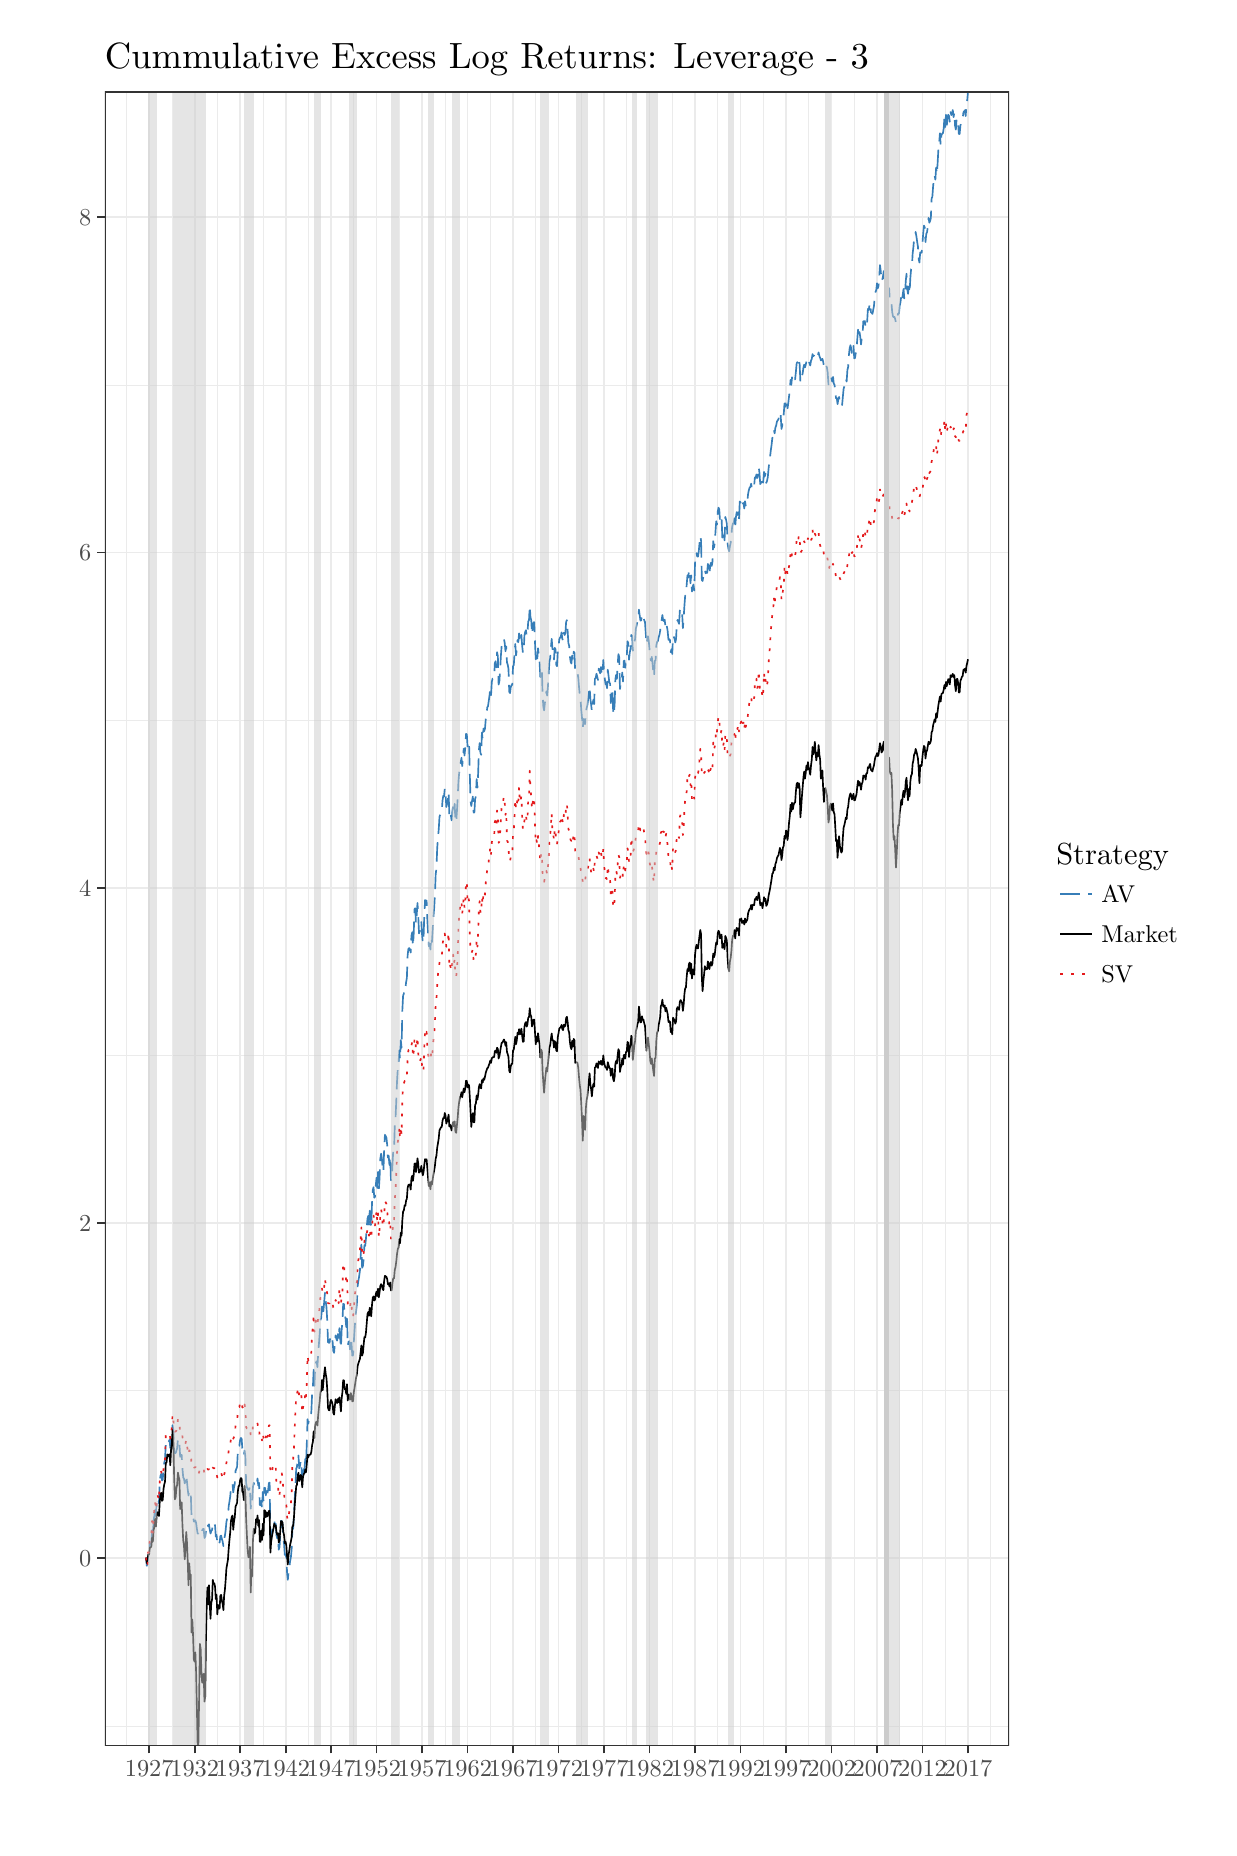
\begin{tikzpicture}[x=1pt,y=1pt]
\definecolor{fillColor}{RGB}{255,255,255}
\path[use as bounding box,fill=fillColor,fill opacity=0.00] (0,0) rectangle (426.79,650.43);
\begin{scope}
\path[clip] (  0.00,  0.00) rectangle (426.79,650.43);
\definecolor{drawColor}{RGB}{255,255,255}
\definecolor{fillColor}{RGB}{255,255,255}

\path[draw=drawColor,line width= 0.6pt,line join=round,line cap=round,fill=fillColor] (  0.00,  0.00) rectangle (426.79,650.43);
\end{scope}
\begin{scope}
\path[clip] ( 27.92, 29.59) rectangle (354.63,627.29);
\definecolor{fillColor}{RGB}{255,255,255}

\path[fill=fillColor] ( 27.92, 29.59) rectangle (354.63,627.29);
\definecolor{drawColor}{gray}{0.92}

\path[draw=drawColor,line width= 0.3pt,line join=round] ( 27.92, 36.76) --
	(354.63, 36.76);

\path[draw=drawColor,line width= 0.3pt,line join=round] ( 27.92,157.90) --
	(354.63,157.90);

\path[draw=drawColor,line width= 0.3pt,line join=round] ( 27.92,279.04) --
	(354.63,279.04);

\path[draw=drawColor,line width= 0.3pt,line join=round] ( 27.92,400.18) --
	(354.63,400.18);

\path[draw=drawColor,line width= 0.3pt,line join=round] ( 27.92,521.32) --
	(354.63,521.32);

\path[draw=drawColor,line width= 0.3pt,line join=round] ( 35.69, 29.59) --
	( 35.69,627.29);

\path[draw=drawColor,line width= 0.3pt,line join=round] ( 52.13, 29.59) --
	( 52.13,627.29);

\path[draw=drawColor,line width= 0.3pt,line join=round] ( 68.57, 29.59) --
	( 68.57,627.29);

\path[draw=drawColor,line width= 0.3pt,line join=round] ( 85.01, 29.59) --
	( 85.01,627.29);

\path[draw=drawColor,line width= 0.3pt,line join=round] (101.45, 29.59) --
	(101.45,627.29);

\path[draw=drawColor,line width= 0.3pt,line join=round] (117.88, 29.59) --
	(117.88,627.29);

\path[draw=drawColor,line width= 0.3pt,line join=round] (134.32, 29.59) --
	(134.32,627.29);

\path[draw=drawColor,line width= 0.3pt,line join=round] (150.77, 29.59) --
	(150.77,627.29);

\path[draw=drawColor,line width= 0.3pt,line join=round] (167.20, 29.59) --
	(167.20,627.29);

\path[draw=drawColor,line width= 0.3pt,line join=round] (183.64, 29.59) --
	(183.64,627.29);

\path[draw=drawColor,line width= 0.3pt,line join=round] (200.08, 29.59) --
	(200.08,627.29);

\path[draw=drawColor,line width= 0.3pt,line join=round] (216.52, 29.59) --
	(216.52,627.29);

\path[draw=drawColor,line width= 0.3pt,line join=round] (232.96, 29.59) --
	(232.96,627.29);

\path[draw=drawColor,line width= 0.3pt,line join=round] (249.39, 29.59) --
	(249.39,627.29);

\path[draw=drawColor,line width= 0.3pt,line join=round] (265.84, 29.59) --
	(265.84,627.29);

\path[draw=drawColor,line width= 0.3pt,line join=round] (282.28, 29.59) --
	(282.28,627.29);

\path[draw=drawColor,line width= 0.3pt,line join=round] (298.71, 29.59) --
	(298.71,627.29);

\path[draw=drawColor,line width= 0.3pt,line join=round] (315.15, 29.59) --
	(315.15,627.29);

\path[draw=drawColor,line width= 0.3pt,line join=round] (331.59, 29.59) --
	(331.59,627.29);

\path[draw=drawColor,line width= 0.3pt,line join=round] (348.03, 29.59) --
	(348.03,627.29);

\path[draw=drawColor,line width= 0.6pt,line join=round] ( 27.92, 97.33) --
	(354.63, 97.33);

\path[draw=drawColor,line width= 0.6pt,line join=round] ( 27.92,218.47) --
	(354.63,218.47);

\path[draw=drawColor,line width= 0.6pt,line join=round] ( 27.92,339.61) --
	(354.63,339.61);

\path[draw=drawColor,line width= 0.6pt,line join=round] ( 27.92,460.75) --
	(354.63,460.75);

\path[draw=drawColor,line width= 0.6pt,line join=round] ( 27.92,581.89) --
	(354.63,581.89);

\path[draw=drawColor,line width= 0.6pt,line join=round] ( 43.91, 29.59) --
	( 43.91,627.29);

\path[draw=drawColor,line width= 0.6pt,line join=round] ( 60.35, 29.59) --
	( 60.35,627.29);

\path[draw=drawColor,line width= 0.6pt,line join=round] ( 76.79, 29.59) --
	( 76.79,627.29);

\path[draw=drawColor,line width= 0.6pt,line join=round] ( 93.23, 29.59) --
	( 93.23,627.29);

\path[draw=drawColor,line width= 0.6pt,line join=round] (109.66, 29.59) --
	(109.66,627.29);

\path[draw=drawColor,line width= 0.6pt,line join=round] (126.10, 29.59) --
	(126.10,627.29);

\path[draw=drawColor,line width= 0.6pt,line join=round] (142.55, 29.59) --
	(142.55,627.29);

\path[draw=drawColor,line width= 0.6pt,line join=round] (158.98, 29.59) --
	(158.98,627.29);

\path[draw=drawColor,line width= 0.6pt,line join=round] (175.42, 29.59) --
	(175.42,627.29);

\path[draw=drawColor,line width= 0.6pt,line join=round] (191.86, 29.59) --
	(191.86,627.29);

\path[draw=drawColor,line width= 0.6pt,line join=round] (208.30, 29.59) --
	(208.30,627.29);

\path[draw=drawColor,line width= 0.6pt,line join=round] (224.74, 29.59) --
	(224.74,627.29);

\path[draw=drawColor,line width= 0.6pt,line join=round] (241.18, 29.59) --
	(241.18,627.29);

\path[draw=drawColor,line width= 0.6pt,line join=round] (257.61, 29.59) --
	(257.61,627.29);

\path[draw=drawColor,line width= 0.6pt,line join=round] (274.06, 29.59) --
	(274.06,627.29);

\path[draw=drawColor,line width= 0.6pt,line join=round] (290.50, 29.59) --
	(290.50,627.29);

\path[draw=drawColor,line width= 0.6pt,line join=round] (306.93, 29.59) --
	(306.93,627.29);

\path[draw=drawColor,line width= 0.6pt,line join=round] (323.37, 29.59) --
	(323.37,627.29);

\path[draw=drawColor,line width= 0.6pt,line join=round] (339.81, 29.59) --
	(339.81,627.29);
\definecolor{drawColor}{RGB}{55,126,184}

\path[draw=drawColor,line width= 0.6pt,dash pattern=on 7pt off 3pt ,line join=round] ( 42.78, 97.57) --
	( 43.05, 94.59) --
	( 43.32, 96.11) --
	( 43.60, 98.48) --
	( 43.87, 98.42) --
	( 44.15,102.56) --
	( 44.43,102.68) --
	( 44.68,103.01) --
	( 44.96,107.53) --
	( 45.23,105.48) --
	( 45.51,111.01) --
	( 45.78,112.72) --
	( 46.06,115.94) --
	( 46.34,112.64) --
	( 46.61,117.38) --
	( 46.89,119.07) --
	( 47.16,118.63) --
	( 47.44,117.17) --
	( 47.72,125.04) --
	( 47.98,127.09) --
	( 48.26,127.84) --
	( 48.53,125.49) --
	( 48.81,125.71) --
	( 49.08,130.18) --
	( 49.36,131.89) --
	( 49.63,132.87) --
	( 49.90,138.80) --
	( 50.18,138.86) --
	( 50.45,140.21) --
	( 50.73,140.17) --
	( 51.01,139.66) --
	( 51.26,140.11) --
	( 51.54,137.20) --
	( 51.81,140.50) --
	( 52.09,142.20) --
	( 52.36,145.46) --
	( 52.64,143.65) --
	( 52.92,135.79) --
	( 53.19,135.30) --
	( 53.47,135.37) --
	( 53.74,136.22) --
	( 54.02,137.15) --
	( 54.30,140.57) --
	( 54.55,139.60) --
	( 54.83,138.82) --
	( 55.10,134.01) --
	( 55.38,134.63) --
	( 55.65,134.66) --
	( 55.93,129.64) --
	( 56.21,126.55) --
	( 56.48,126.09) --
	( 56.75,124.42) --
	( 57.02,125.43) --
	( 57.30,127.39) --
	( 57.58,124.84) --
	( 57.83,122.24) --
	( 58.11,120.05) --
	( 58.38,121.80) --
	( 58.66,121.14) --
	( 58.93,121.20) --
	( 59.21,112.46) --
	( 59.49,113.21) --
	( 59.76,112.74) --
	( 60.04,110.65) --
	( 60.31,110.57) --
	( 60.59,111.03) --
	( 60.87,110.06) --
	( 61.13,108.12) --
	( 61.41,106.31) --
	( 61.68,106.27) --
	( 61.96,107.69) --
	( 62.23,108.33) --
	( 62.51,108.18) --
	( 62.79,107.75) --
	( 63.06,107.48) --
	( 63.33,107.90) --
	( 63.60,107.99) --
	( 63.88,104.68) --
	( 64.16,105.14) --
	( 64.41,107.10) --
	( 64.69,108.51) --
	( 64.96,109.81) --
	( 65.24,108.88) --
	( 65.51,109.62) --
	( 65.79,107.69) --
	( 66.07,106.31) --
	( 66.34,107.20) --
	( 66.62,107.51) --
	( 66.89,110.23) --
	( 67.17,109.67) --
	( 67.45,109.78) --
	( 67.70,109.21) --
	( 67.98,105.23) --
	( 68.25,105.84) --
	( 68.53,102.58) --
	( 68.80,103.64) --
	( 69.08,103.58) --
	( 69.36,102.99) --
	( 69.63,105.39) --
	( 69.91,105.53) --
	( 70.18,104.31) --
	( 70.45,103.38) --
	( 70.73,101.73) --
	( 70.99,104.25) --
	( 71.26,105.48) --
	( 71.53,107.40) --
	( 71.81,110.42) --
	( 72.08,111.76) --
	( 72.36,112.57) --
	( 72.64,116.13) --
	( 72.91,117.81) --
	( 73.19,119.69) --
	( 73.46,122.71) --
	( 73.74,123.84) --
	( 74.02,124.26) --
	( 74.28,121.15) --
	( 74.56,123.00) --
	( 74.83,124.20) --
	( 75.11,128.89) --
	( 75.38,129.60) --
	( 75.66,130.34) --
	( 75.94,135.88) --
	( 76.21,137.91) --
	( 76.49,138.02) --
	( 76.76,140.03) --
	( 77.03,140.82) --
	( 77.31,140.61) --
	( 77.57,136.91) --
	( 77.84,136.65) --
	( 78.11,134.52) --
	( 78.39,136.28) --
	( 78.66,134.14) --
	( 78.94,124.46) --
	( 79.22,122.97) --
	( 79.49,122.39) --
	( 79.77,121.99) --
	( 80.04,122.17) --
	( 80.32,123.46) --
	( 80.60,115.27) --
	( 80.85,117.89) --
	( 81.13,117.32) --
	( 81.40,123.09) --
	( 81.68,124.60) --
	( 81.95,123.82) --
	( 82.23,123.93) --
	( 82.51,125.04) --
	( 82.78,124.39) --
	( 83.06,126.19) --
	( 83.33,123.63) --
	( 83.61,124.64) --
	( 83.88,116.62) --
	( 84.14,116.56) --
	( 84.42,118.15) --
	( 84.69,115.20) --
	( 84.96,121.30) --
	( 85.23,117.87) --
	( 85.51,122.81) --
	( 85.79,122.76) --
	( 86.06,120.05) --
	( 86.34,122.78) --
	( 86.61,120.76) --
	( 86.89,122.07) --
	( 87.17,124.59) --
	( 87.43,124.67) --
	( 87.71,104.92) --
	( 87.98,105.70) --
	( 88.26,106.37) --
	( 88.53,108.11) --
	( 88.81,109.25) --
	( 89.09,110.76) --
	( 89.36,109.58) --
	( 89.64,109.81) --
	( 89.91,105.63) --
	( 90.19,104.55) --
	( 90.46,105.16) --
	( 90.72,100.45) --
	( 91.00,101.33) --
	( 91.27,105.55) --
	( 91.54,110.83) --
	( 91.81,110.74) --
	( 92.09,109.79) --
	( 92.37,104.39) --
	( 92.64,102.64) --
	( 92.92, 98.54) --
	( 93.19, 98.75) --
	( 93.47, 97.58) --
	( 93.75, 91.88) --
	( 94.00, 89.56) --
	( 94.28, 92.48) --
	( 94.55, 94.00) --
	( 94.83, 96.37) --
	( 95.10, 97.65) --
	( 95.38,100.53) --
	( 95.66,107.97) --
	( 95.93,108.03) --
	( 96.21,112.61) --
	( 96.48,118.20) --
	( 96.76,123.77) --
	( 97.04,129.75) --
	( 97.29,130.25) --
	( 97.57,133.30) --
	( 97.84,134.48) --
	( 98.12,129.84) --
	( 98.39,130.73) --
	( 98.67,132.62) --
	( 98.94,131.11) --
	( 99.21,123.76) --
	( 99.49,127.88) --
	( 99.76,129.41) --
	(100.04,129.81) --
	(100.32,133.25) --
	(100.58,131.24) --
	(100.86,138.64) --
	(101.13,147.61) --
	(101.41,145.99) --
	(101.68,147.59) --
	(101.96,147.61) --
	(102.24,147.81) --
	(102.51,150.51) --
	(102.79,156.99) --
	(103.06,159.09) --
	(103.34,165.49) --
	(103.62,159.65) --
	(103.87,166.12) --
	(104.15,168.05) --
	(104.42,168.51) --
	(104.70,166.39) --
	(104.97,171.39) --
	(105.25,174.86) --
	(105.52,178.58) --
	(105.79,183.33) --
	(106.07,184.23) --
	(106.34,188.31) --
	(106.62,184.86) --
	(106.90,187.16) --
	(107.15,190.08) --
	(107.43,193.28) --
	(107.70,190.19) --
	(107.98,187.99) --
	(108.25,183.18) --
	(108.53,175.45) --
	(108.81,175.22) --
	(109.08,175.23) --
	(109.36,177.37) --
	(109.63,177.87) --
	(109.91,177.14) --
	(110.19,175.61) --
	(110.44,172.26) --
	(110.72,171.58) --
	(110.99,174.77) --
	(111.27,177.89) --
	(111.54,176.57) --
	(111.82,176.01) --
	(112.10,178.39) --
	(112.37,176.42) --
	(112.64,180.52) --
	(112.91,177.20) --
	(113.19,173.28) --
	(113.47,180.09) --
	(113.73,182.71) --
	(114.01,189.29) --
	(114.28,189.20) --
	(114.56,184.23) --
	(114.83,184.44) --
	(115.11,180.93) --
	(115.39,185.49) --
	(115.66,174.19) --
	(115.94,175.54) --
	(116.21,175.79) --
	(116.49,172.81) --
	(116.77,176.93) --
	(117.02,174.92) --
	(117.30,170.54) --
	(117.57,170.71) --
	(117.85,175.52) --
	(118.12,179.91) --
	(118.40,183.75) --
	(118.68,186.70) --
	(118.95,189.08) --
	(119.22,195.60) --
	(119.49,197.58) --
	(119.77,199.17) --
	(120.05,201.19) --
	(120.30,206.06) --
	(120.58,210.72) --
	(120.85,202.30) --
	(121.13,202.91) --
	(121.40,205.39) --
	(121.68,210.49) --
	(121.96,210.24) --
	(122.23,212.75) --
	(122.51,216.63) --
	(122.78,220.04) --
	(123.06,221.07) --
	(123.34,217.88) --
	(123.59,222.92) --
	(123.87,219.84) --
	(124.14,217.00) --
	(124.42,225.56) --
	(124.69,230.37) --
	(124.97,231.42) --
	(125.25,227.63) --
	(125.52,228.04) --
	(125.80,232.17) --
	(126.07,234.87) --
	(126.34,231.13) --
	(126.62,236.99) --
	(126.88,230.34) --
	(127.16,234.87) --
	(127.43,241.71) --
	(127.71,243.53) --
	(127.98,242.03) --
	(128.26,238.25) --
	(128.54,237.01) --
	(128.81,245.06) --
	(129.09,250.37) --
	(129.36,249.89) --
	(129.64,249.27) --
	(129.92,246.62) --
	(130.17,242.11) --
	(130.45,242.76) --
	(130.72,239.47) --
	(131.00,242.47) --
	(131.27,233.95) --
	(131.55,234.23) --
	(131.83,239.82) --
	(132.10,244.63) --
	(132.38,244.52) --
	(132.65,253.44) --
	(132.92,256.36) --
	(133.20,262.83) --
	(133.46,269.63) --
	(133.73,274.14) --
	(134.00,275.92) --
	(134.28,280.87) --
	(134.55,277.66) --
	(134.83,284.52) --
	(135.11,281.81) --
	(135.38,295.20) --
	(135.66,300.69) --
	(135.93,301.37) --
	(136.21,303.53) --
	(136.49,303.29) --
	(136.74,305.46) --
	(137.02,307.02) --
	(137.29,315.15) --
	(137.57,317.58) --
	(137.84,317.84) --
	(138.12,317.44) --
	(138.40,316.20) --
	(138.67,322.24) --
	(138.95,323.56) --
	(139.22,318.52) --
	(139.50,323.17) --
	(139.77,331.85) --
	(140.04,332.23) --
	(140.31,326.74) --
	(140.58,329.80) --
	(140.86,334.16) --
	(141.13,329.54) --
	(141.41,323.14) --
	(141.69,323.98) --
	(141.96,324.28) --
	(142.24,327.25) --
	(142.51,322.71) --
	(142.79,319.70) --
	(143.07,322.26) --
	(143.32,329.85) --
	(143.60,335.19) --
	(143.87,334.20) --
	(144.15,335.02) --
	(144.42,328.12) --
	(144.70,323.02) --
	(144.98,318.44) --
	(145.25,319.32) --
	(145.53,317.33) --
	(145.80,321.73) --
	(146.08,319.97) --
	(146.35,324.49) --
	(146.61,329.03) --
	(146.89,332.28) --
	(147.16,337.12) --
	(147.43,344.42) --
	(147.71,346.79) --
	(147.98,353.90) --
	(148.26,357.75) --
	(148.53,360.63) --
	(148.81,365.33) --
	(149.08,366.02) --
	(149.36,367.03) --
	(149.64,367.34) --
	(149.89,371.06) --
	(150.17,372.83) --
	(150.44,372.69) --
	(150.72,375.48) --
	(150.99,373.98) --
	(151.27,368.82) --
	(151.55,369.94) --
	(151.82,371.48) --
	(152.10,374.10) --
	(152.37,365.95) --
	(152.65,367.27) --
	(152.93,365.70) --
	(153.19,363.98) --
	(153.47,367.37) --
	(153.74,369.22) --
	(154.02,367.21) --
	(154.29,369.97) --
	(154.56,363.85) --
	(154.84,363.34) --
	(155.11,367.23) --
	(155.39,372.23) --
	(155.66,378.12) --
	(155.94,381.32) --
	(156.22,384.45) --
	(156.47,384.84) --
	(156.75,386.60) --
	(157.02,383.58) --
	(157.30,386.89) --
	(157.57,389.90) --
	(157.85,387.43) --
	(158.13,390.31) --
	(158.40,395.23) --
	(158.68,395.10) --
	(158.95,390.69) --
	(159.23,392.41) --
	(159.51,391.32) --
	(159.76,380.61) --
	(160.04,370.89) --
	(160.31,369.17) --
	(160.59,371.10) --
	(160.86,372.60) --
	(161.14,366.82) --
	(161.41,366.81) --
	(161.68,371.75) --
	(161.96,372.64) --
	(162.23,378.90) --
	(162.51,375.80) --
	(162.79,381.24) --
	(163.04,389.24) --
	(163.32,391.92) --
	(163.59,388.44) --
	(163.87,387.69) --
	(164.14,395.74) --
	(164.42,393.17) --
	(164.70,397.16) --
	(164.97,396.23) --
	(165.25,397.15) --
	(165.52,400.49) --
	(165.80,402.24) --
	(166.08,404.87) --
	(166.34,405.22) --
	(166.62,407.20) --
	(166.89,409.17) --
	(167.17,411.83) --
	(167.44,409.25) --
	(167.72,414.10) --
	(167.99,415.19) --
	(168.26,415.25) --
	(168.54,415.39) --
	(168.81,420.80) --
	(169.09,421.49) --
	(169.37,419.28) --
	(169.62,424.75) --
	(169.90,423.31) --
	(170.17,413.07) --
	(170.45,414.23) --
	(170.72,418.37) --
	(171.00,423.53) --
	(171.28,427.19) --
	(171.55,427.18) --
	(171.83,428.61) --
	(172.10,429.48) --
	(172.38,428.04) --
	(172.66,425.07) --
	(172.91,426.80) --
	(173.19,421.07) --
	(173.46,420.28) --
	(173.74,418.68) --
	(174.01,410.46) --
	(174.29,409.97) --
	(174.57,412.22) --
	(174.84,412.82) --
	(175.11,412.96) --
	(175.38,419.65) --
	(175.66,420.19) --
	(175.94,424.43) --
	(176.19,427.71) --
	(176.47,423.59) --
	(176.74,425.66) --
	(177.02,429.13) --
	(177.29,428.34) --
	(177.57,431.56) --
	(177.85,428.48) --
	(178.12,428.90) --
	(178.40,430.99) --
	(178.67,427.24) --
	(178.95,424.55) --
	(179.23,424.64) --
	(179.49,430.70) --
	(179.77,432.08) --
	(180.04,432.69) --
	(180.32,430.59) --
	(180.59,431.64) --
	(180.87,435.84) --
	(181.15,436.33) --
	(181.42,441.50) --
	(181.69,437.33) --
	(181.96,436.30) --
	(182.24,431.31) --
	(182.52,433.99) --
	(182.77,435.53) --
	(183.05,435.57) --
	(183.32,428.31) --
	(183.60,422.15) --
	(183.87,424.56) --
	(184.15,422.45) --
	(184.43,426.17) --
	(184.70,423.61) --
	(184.98,421.05) --
	(185.25,415.75) --
	(185.53,418.79) --
	(185.81,418.17) --
	(186.06,409.41) --
	(186.34,404.98) --
	(186.61,403.72) --
	(186.89,406.38) --
	(187.16,408.36) --
	(187.44,410.57) --
	(187.72,409.05) --
	(187.99,412.27) --
	(188.27,417.11) --
	(188.54,421.47) --
	(188.81,422.58) --
	(189.09,426.65) --
	(189.35,429.58) --
	(189.62,425.86) --
	(189.89,425.90) --
	(190.17,422.09) --
	(190.44,426.34) --
	(190.72,425.87) --
	(191.00,420.19) --
	(191.27,419.70) --
	(191.55,424.99) --
	(191.82,426.76) --
	(192.10,429.42) --
	(192.38,430.04) --
	(192.64,430.33) --
	(192.92,431.91) --
	(193.19,429.59) --
	(193.47,428.76) --
	(193.74,431.81) --
	(194.02,430.96) --
	(194.30,431.65) --
	(194.57,435.68) --
	(194.85,436.35) --
	(195.12,432.34) --
	(195.39,427.99) --
	(195.67,427.09) --
	(195.93,423.23) --
	(196.20,421.30) --
	(196.47,420.67) --
	(196.75,423.57) --
	(197.02,421.68) --
	(197.30,424.97) --
	(197.58,424.50) --
	(197.85,417.24) --
	(198.13,417.41) --
	(198.40,417.38) --
	(198.68,417.25) --
	(198.96,415.54) --
	(199.21,412.37) --
	(199.49,409.47) --
	(199.76,408.10) --
	(200.04,403.88) --
	(200.31,400.98) --
	(200.59,397.31) --
	(200.87,400.63) --
	(201.14,399.81) --
	(201.42,398.72) --
	(201.69,403.07) --
	(201.97,404.52) --
	(202.24,405.56) --
	(202.50,407.52) --
	(202.78,409.84) --
	(203.05,412.30) --
	(203.32,407.90) --
	(203.60,405.86) --
	(203.87,403.39) --
	(204.15,406.13) --
	(204.42,407.57) --
	(204.70,406.04) --
	(204.97,415.20) --
	(205.25,415.36) --
	(205.53,416.98) --
	(205.79,415.98) --
	(206.07,414.72) --
	(206.34,418.81) --
	(206.62,417.84) --
	(206.89,417.12) --
	(207.17,419.43) --
	(207.45,416.46) --
	(207.72,416.56) --
	(208.00,421.94) --
	(208.27,417.36) --
	(208.55,415.05) --
	(208.82,413.17) --
	(209.08,413.35) --
	(209.36,411.75) --
	(209.63,418.41) --
	(209.91,416.06) --
	(210.18,413.79) --
	(210.45,413.45) --
	(210.73,406.34) --
	(211.00,411.28) --
	(211.28,411.60) --
	(211.55,403.77) --
	(211.83,402.08) --
	(212.11,406.28) --
	(212.36,414.98) --
	(212.64,416.53) --
	(212.91,415.09) --
	(213.19,420.13) --
	(213.46,424.03) --
	(213.74,423.06) --
	(214.02,411.44) --
	(214.29,413.33) --
	(214.57,413.91) --
	(214.84,417.39) --
	(215.12,414.14) --
	(215.40,421.57) --
	(215.65,421.70) --
	(215.93,419.09) --
	(216.20,422.62) --
	(216.48,423.28) --
	(216.75,428.69) --
	(217.03,428.04) --
	(217.30,422.04) --
	(217.57,424.69) --
	(217.85,426.01) --
	(218.12,430.99) --
	(218.40,430.67) --
	(218.68,425.29) --
	(218.94,426.38) --
	(219.22,428.22) --
	(219.49,429.61) --
	(219.77,433.34) --
	(220.04,434.39) --
	(220.32,435.88) --
	(220.60,436.43) --
	(220.87,440.13) --
	(221.15,438.02) --
	(221.42,436.14) --
	(221.70,436.27) --
	(221.98,438.31) --
	(222.23,437.40) --
	(222.51,437.47) --
	(222.78,436.28) --
	(223.06,435.68) --
	(223.33,431.79) --
	(223.61,427.74) --
	(223.88,429.39) --
	(224.15,430.52) --
	(224.43,428.74) --
	(224.70,425.87) --
	(224.98,422.84) --
	(225.26,421.70) --
	(225.51,423.07) --
	(225.79,420.64) --
	(226.06,417.63) --
	(226.34,415.97) --
	(226.61,421.66) --
	(226.89,421.83) --
	(227.17,427.32) --
	(227.44,428.48) --
	(227.72,428.76) --
	(227.99,430.13) --
	(228.27,430.96) --
	(228.55,432.49) --
	(228.80,435.85) --
	(229.08,436.28) --
	(229.35,438.19) --
	(229.63,436.21) --
	(229.90,436.02) --
	(230.18,436.52) --
	(230.46,433.91) --
	(230.73,435.22) --
	(231.00,433.89) --
	(231.27,432.28) --
	(231.55,429.18) --
	(231.83,429.46) --
	(232.09,429.19) --
	(232.37,424.76) --
	(232.64,425.84) --
	(232.92,424.10) --
	(233.19,430.63) --
	(233.47,430.28) --
	(233.75,429.58) --
	(234.02,428.27) --
	(234.30,429.59) --
	(234.57,435.69) --
	(234.85,436.40) --
	(235.13,435.66) --
	(235.38,435.00) --
	(235.66,439.84) --
	(235.93,440.66) --
	(236.21,439.98) --
	(236.48,439.13) --
	(236.76,433.42) --
	(237.04,437.19) --
	(237.31,441.50) --
	(237.58,445.12) --
	(237.85,445.38) --
	(238.13,449.15) --
	(238.41,452.50) --
	(238.66,451.68) --
	(238.94,453.89) --
	(239.21,454.55) --
	(239.49,449.65) --
	(239.76,452.53) --
	(240.04,446.67) --
	(240.32,448.49) --
	(240.59,449.22) --
	(240.87,447.03) --
	(241.14,456.91) --
	(241.42,459.26) --
	(241.70,460.56) --
	(241.95,459.28) --
	(242.23,459.29) --
	(242.50,461.21) --
	(242.78,464.28) --
	(243.05,466.72) --
	(243.33,465.06) --
	(243.61,450.82) --
	(243.88,450.49) --
	(244.16,452.21) --
	(244.43,453.33) --
	(244.70,454.49) --
	(244.98,453.25) --
	(245.24,453.62) --
	(245.52,453.39) --
	(245.79,456.65) --
	(246.07,455.78) --
	(246.34,452.87) --
	(246.62,455.91) --
	(246.90,457.07) --
	(247.17,455.92) --
	(247.45,457.40) --
	(247.72,464.89) --
	(248.00,462.54) --
	(248.28,464.28) --
	(248.53,468.17) --
	(248.81,472.07) --
	(249.08,470.86) --
	(249.36,475.56) --
	(249.63,476.99) --
	(249.91,476.31) --
	(250.19,471.86) --
	(250.46,472.26) --
	(250.74,473.36) --
	(251.01,466.14) --
	(251.28,466.65) --
	(251.56,468.34) --
	(251.82,465.15) --
	(252.09,473.63) --
	(252.36,472.59) --
	(252.64,471.18) --
	(252.91,464.09) --
	(253.19,462.23) --
	(253.47,461.18) --
	(253.74,463.00) --
	(254.02,464.19) --
	(254.29,467.28) --
	(254.57,470.17) --
	(254.85,471.30) --
	(255.10,471.21) --
	(255.38,473.17) --
	(255.65,469.77) --
	(255.93,473.58) --
	(256.20,475.35) --
	(256.48,474.30) --
	(256.76,475.62) --
	(257.03,472.82) --
	(257.31,479.21) --
	(257.58,478.92) --
	(257.86,479.38) --
	(258.13,477.47) --
	(258.40,478.51) --
	(258.67,478.67) --
	(258.94,476.68) --
	(259.22,479.30) --
	(259.49,477.44) --
	(259.77,478.50) --
	(260.05,479.23) --
	(260.32,481.93) --
	(260.60,483.33) --
	(260.87,484.23) --
	(261.15,484.43) --
	(261.43,485.68) --
	(261.68,483.75) --
	(261.96,484.98) --
	(262.23,485.22) --
	(262.51,485.00) --
	(262.78,487.89) --
	(263.06,487.75) --
	(263.34,488.98) --
	(263.61,487.66) --
	(263.89,488.82) --
	(264.16,491.61) --
	(264.44,489.51) --
	(264.71,485.48) --
	(264.97,485.97) --
	(265.25,486.32) --
	(265.52,484.38) --
	(265.80,486.45) --
	(266.07,489.91) --
	(266.34,488.25) --
	(266.62,489.31) --
	(266.89,485.93) --
	(267.17,486.65) --
	(267.44,488.04) --
	(267.72,491.09) --
	(268.00,493.48) --
	(268.25,495.26) --
	(268.53,497.73) --
	(268.80,499.63) --
	(269.08,502.17) --
	(269.35,502.46) --
	(269.63,505.13) --
	(269.91,503.83) --
	(270.18,505.93) --
	(270.46,506.59) --
	(270.73,508.04) --
	(271.01,508.52) --
	(271.29,508.95) --
	(271.55,510.02) --
	(271.83,511.38) --
	(272.10,510.46) --
	(272.38,505.42) --
	(272.65,506.59) --
	(272.92,509.96) --
	(273.20,510.73) --
	(273.47,514.64) --
	(273.75,513.46) --
	(274.02,516.16) --
	(274.30,515.86) --
	(274.58,512.87) --
	(274.83,514.69) --
	(275.11,517.10) --
	(275.38,519.27) --
	(275.66,523.16) --
	(275.93,521.34) --
	(276.21,524.10) --
	(276.49,522.10) --
	(276.76,522.69) --
	(277.04,523.34) --
	(277.31,523.37) --
	(277.59,526.05) --
	(277.87,529.16) --
	(278.12,529.55) --
	(278.40,528.38) --
	(278.67,530.09) --
	(278.95,528.86) --
	(279.22,522.27) --
	(279.50,523.53) --
	(279.77,524.64) --
	(280.04,525.49) --
	(280.32,527.67) --
	(280.59,528.64) --
	(280.87,527.67) --
	(281.15,528.62) --
	(281.40,529.84) --
	(281.68,529.42) --
	(281.95,530.66) --
	(282.23,529.71) --
	(282.50,529.16) --
	(282.78,528.34) --
	(283.06,530.08) --
	(283.33,530.72) --
	(283.61,532.47) --
	(283.88,531.68) --
	(284.16,531.97) --
	(284.44,532.66) --
	(284.70,532.05) --
	(284.98,531.71) --
	(285.25,532.32) --
	(285.53,531.98) --
	(285.80,533.10) --
	(286.08,531.75) --
	(286.35,531.16) --
	(286.62,530.17) --
	(286.90,530.39) --
	(287.17,530.76) --
	(287.45,529.74) --
	(287.73,527.89) --
	(287.98,528.96) --
	(288.26,529.04) --
	(288.53,528.36) --
	(288.81,527.57) --
	(289.08,525.77) --
	(289.36,521.50) --
	(289.64,521.98) --
	(289.91,523.63) --
	(290.19,524.25) --
	(290.46,523.45) --
	(290.74,522.54) --
	(291.02,524.22) --
	(291.27,521.85) --
	(291.55,521.39) --
	(291.82,519.11) --
	(292.10,516.52) --
	(292.37,516.59) --
	(292.65,514.39) --
	(292.93,516.20) --
	(293.20,516.98) --
	(293.47,515.42) --
	(293.74,514.16) --
	(294.02,513.60) --
	(294.30,514.15) --
	(294.55,516.89) --
	(294.83,519.90) --
	(295.10,520.75) --
	(295.38,522.12) --
	(295.65,523.50) --
	(295.93,522.56) --
	(296.21,526.74) --
	(296.48,527.84) --
	(296.76,532.28) --
	(297.03,534.64) --
	(297.31,535.68) --
	(297.59,534.48) --
	(297.85,532.53) --
	(298.13,533.48) --
	(298.40,535.45) --
	(298.68,530.91) --
	(298.95,531.07) --
	(299.23,532.82) --
	(299.51,534.51) --
	(299.78,537.92) --
	(300.05,541.30) --
	(300.32,538.26) --
	(300.60,540.40) --
	(300.88,538.45) --
	(301.13,535.96) --
	(301.41,538.42) --
	(301.68,539.50) --
	(301.96,544.39) --
	(302.23,543.52) --
	(302.51,544.44) --
	(302.79,541.95) --
	(303.06,544.08) --
	(303.34,544.15) --
	(303.61,548.78) --
	(303.89,548.41) --
	(304.17,549.98) --
	(304.42,550.98) --
	(304.70,547.65) --
	(304.97,547.37) --
	(305.25,546.99) --
	(305.52,548.37) --
	(305.80,549.85) --
	(306.08,553.10) --
	(306.35,554.88) --
	(306.63,555.59) --
	(306.90,558.05) --
	(307.17,556.22) --
	(307.45,557.08) --
	(307.71,560.55) --
	(307.98,564.62) --
	(308.25,562.54) --
	(308.53,558.90) --
	(308.80,559.38) --
	(309.08,560.65) --
	(309.36,562.47) --
	(309.63,559.65) --
	(309.91,559.44) --
	(310.18,555.46) --
	(310.46,554.81) --
	(310.74,554.33) --
	(311.00,555.51) --
	(311.28,556.31) --
	(311.55,551.76) --
	(311.83,551.12) --
	(312.10,551.26) --
	(312.38,547.78) --
	(312.66,546.13) --
	(312.93,545.79) --
	(313.21,545.92) --
	(313.48,545.09) --
	(313.75,543.80) --
	(314.03,545.22) --
	(314.29,546.16) --
	(314.56,547.19) --
	(314.84,547.13) --
	(315.11,550.02) --
	(315.38,551.15) --
	(315.66,553.42) --
	(315.94,551.80) --
	(316.21,554.01) --
	(316.49,556.00) --
	(316.76,552.59) --
	(317.04,554.84) --
	(317.32,559.15) --
	(317.57,561.51) --
	(317.85,555.87) --
	(318.12,554.25) --
	(318.40,556.95) --
	(318.67,554.47) --
	(318.95,560.05) --
	(319.23,563.20) --
	(319.50,563.63) --
	(319.78,568.70) --
	(320.05,571.11) --
	(320.33,574.37) --
	(320.60,574.66) --
	(320.86,576.62) --
	(321.14,574.97) --
	(321.41,573.08) --
	(321.69,571.37) --
	(321.96,566.86) --
	(322.23,565.55) --
	(322.51,569.22) --
	(322.78,569.05) --
	(323.06,569.16) --
	(323.33,572.65) --
	(323.61,576.24) --
	(323.89,578.91) --
	(324.15,578.22) --
	(324.43,572.93) --
	(324.70,575.92) --
	(324.98,576.52) --
	(325.25,578.39) --
	(325.53,581.70) --
	(325.81,579.95) --
	(326.08,580.57) --
	(326.36,581.62) --
	(326.63,588.60) --
	(326.91,589.41) --
	(327.19,593.25) --
	(327.44,595.68) --
	(327.72,596.99) --
	(327.99,595.50) --
	(328.27,599.88) --
	(328.54,597.48) --
	(328.81,601.54) --
	(329.09,606.64) --
	(329.36,608.81) --
	(329.64,612.27) --
	(329.91,607.97) --
	(330.19,611.63) --
	(330.47,612.10) --
	(330.72,612.30) --
	(331.00,613.96) --
	(331.27,618.04) --
	(331.55,614.52) --
	(331.82,618.93) --
	(332.10,614.77) --
	(332.38,617.81) --
	(332.65,618.97) --
	(332.93,618.49) --
	(333.20,616.43) --
	(333.48,619.92) --
	(333.76,618.82) --
	(334.01,619.55) --
	(334.29,620.66) --
	(334.56,618.10) --
	(334.84,619.69) --
	(335.11,615.00) --
	(335.39,613.59) --
	(335.66,617.39) --
	(335.93,617.54) --
	(336.21,615.60) --
	(336.48,611.99) --
	(336.76,612.01) --
	(337.04,615.01) --
	(337.30,616.04) --
	(337.58,617.19) --
	(337.85,617.50) --
	(338.13,619.82) --
	(338.40,620.16) --
	(338.68,620.59) --
	(338.96,618.46) --
	(339.23,623.12) --
	(339.51,624.25) --
	(339.78,627.29);
\definecolor{drawColor}{RGB}{0,0,0}

\path[draw=drawColor,line width= 0.6pt,line join=round] ( 42.78, 97.55) --
	( 43.05, 95.61) --
	( 43.32, 97.18) --
	( 43.60, 98.73) --
	( 43.87, 98.69) --
	( 44.15,101.21) --
	( 44.43,101.28) --
	( 44.68,101.56) --
	( 44.96,104.78) --
	( 45.23,103.34) --
	( 45.51,107.55) --
	( 45.78,108.74) --
	( 46.06,111.51) --
	( 46.34,108.82) --
	( 46.61,112.71) --
	( 46.89,113.98) --
	( 47.16,113.65) --
	( 47.44,112.63) --
	( 47.72,117.73) --
	( 47.98,120.13) --
	( 48.26,121.01) --
	( 48.53,118.08) --
	( 48.81,118.45) --
	( 49.08,122.37) --
	( 49.36,124.06) --
	( 49.63,125.02) --
	( 49.90,131.80) --
	( 50.18,131.89) --
	( 50.45,134.84) --
	( 50.73,134.78) --
	( 51.01,134.10) --
	( 51.26,134.91) --
	( 51.54,130.96) --
	( 51.81,136.60) --
	( 52.09,139.06) --
	( 52.36,143.70) --
	( 52.64,140.37) --
	( 52.92,126.86) --
	( 53.19,118.64) --
	( 53.47,119.35) --
	( 53.74,122.57) --
	( 54.02,124.03) --
	( 54.30,128.30) --
	( 54.55,126.87) --
	( 54.83,125.80) --
	( 55.10,115.11) --
	( 55.38,117.45) --
	( 55.65,117.50) --
	( 55.93,109.31) --
	( 56.21,103.77) --
	( 56.48,101.91) --
	( 56.75, 96.96) --
	( 57.02,100.62) --
	( 57.30,106.84) --
	( 57.58,102.82) --
	( 57.83, 96.40) --
	( 58.11, 87.62) --
	( 58.38, 95.52) --
	( 58.66, 91.30) --
	( 58.93, 91.44) --
	( 59.21, 70.51) --
	( 59.49, 75.24) --
	( 59.76, 69.62) --
	( 60.04, 60.77) --
	( 60.31, 60.03) --
	( 60.59, 63.35) --
	( 60.87, 56.11) --
	( 61.13, 44.00) --
	( 61.41, 29.91) --
	( 61.68, 29.59) --
	( 61.96, 47.31) --
	( 62.23, 66.42) --
	( 62.51, 64.65) --
	( 62.79, 56.01) --
	( 63.06, 52.36) --
	( 63.33, 55.03) --
	( 63.60, 55.61) --
	( 63.88, 45.53) --
	( 64.16, 47.49) --
	( 64.41, 67.64) --
	( 64.69, 79.32) --
	( 64.96, 86.85) --
	( 65.24, 80.69) --
	( 65.51, 87.61) --
	( 65.79, 80.82) --
	( 66.07, 75.51) --
	( 66.34, 81.27) --
	( 66.62, 82.33) --
	( 66.89, 89.55) --
	( 67.17, 88.05) --
	( 67.45, 88.29) --
	( 67.70, 87.15) --
	( 67.98, 82.60) --
	( 68.25, 84.11) --
	( 68.53, 77.08) --
	( 68.80, 80.44) --
	( 69.08, 80.29) --
	( 69.36, 79.13) --
	( 69.63, 83.90) --
	( 69.91, 84.11) --
	( 70.18, 82.05) --
	( 70.45, 80.85) --
	( 70.73, 78.62) --
	( 70.99, 83.85) --
	( 71.26, 85.91) --
	( 71.53, 89.30) --
	( 71.81, 93.63) --
	( 72.08, 95.22) --
	( 72.36, 96.78) --
	( 72.64,100.84) --
	( 72.91,103.95) --
	( 73.19,106.72) --
	( 73.46,110.79) --
	( 73.74,112.30) --
	( 74.02,112.79) --
	( 74.28,107.64) --
	( 74.56,110.70) --
	( 74.83,112.16) --
	( 75.11,116.02) --
	( 75.38,116.66) --
	( 75.66,117.37) --
	( 75.94,121.45) --
	( 76.21,123.41) --
	( 76.49,123.56) --
	( 76.76,125.54) --
	( 77.03,126.33) --
	( 77.31,126.16) --
	( 77.57,121.40) --
	( 77.84,120.96) --
	( 78.11,118.36) --
	( 78.39,123.53) --
	( 78.66,120.51) --
	( 78.94,111.59) --
	( 79.22,105.48) --
	( 79.49,100.20) --
	( 79.77, 97.67) --
	( 80.04, 98.07) --
	( 80.32,101.48) --
	( 80.60, 84.99) --
	( 80.85, 93.24) --
	( 81.13, 90.83) --
	( 81.40,103.75) --
	( 81.68,107.97) --
	( 81.95,106.30) --
	( 82.23,106.85) --
	( 82.51,111.45) --
	( 82.78,110.32) --
	( 83.06,112.80) --
	( 83.33,109.07) --
	( 83.61,111.17) --
	( 83.88,103.38) --
	( 84.14,103.26) --
	( 84.42,107.30) --
	( 84.69,103.96) --
	( 84.96,109.85) --
	( 85.23,105.63) --
	( 85.51,114.71) --
	( 85.79,114.47) --
	( 86.06,112.17) --
	( 86.34,113.94) --
	( 86.61,112.46) --
	( 86.89,113.34) --
	( 87.17,114.46) --
	( 87.43,114.51) --
	( 87.71, 99.38) --
	( 87.98,103.30) --
	( 88.26,105.21) --
	( 88.53,106.67) --
	( 88.81,108.04) --
	( 89.09,109.85) --
	( 89.36,108.83) --
	( 89.64,109.22) --
	( 89.91,106.67) --
	( 90.19,105.83) --
	( 90.46,106.41) --
	( 90.72,103.05) --
	( 91.00,103.84) --
	( 91.27,107.29) --
	( 91.54,110.79) --
	( 91.81,110.72) --
	( 92.09,110.24) --
	( 92.37,106.94) --
	( 92.64,105.69) --
	( 92.92,102.80) --
	( 93.19,103.34) --
	( 93.47,101.88) --
	( 93.75, 97.79) --
	( 94.00, 95.09) --
	( 94.28, 98.62) --
	( 94.55,100.15) --
	( 94.83,102.24) --
	( 95.10,103.33) --
	( 95.38,104.93) --
	( 95.66,108.96) --
	( 95.93,109.01) --
	( 96.21,112.02) --
	( 96.48,116.29) --
	( 96.76,119.83) --
	( 97.04,123.45) --
	( 97.29,123.87) --
	( 97.57,127.22) --
	( 97.84,128.24) --
	( 98.12,125.26) --
	( 98.39,126.05) --
	( 98.67,127.47) --
	( 98.94,126.75) --
	( 99.21,122.99) --
	( 99.49,126.74) --
	( 99.76,127.81) --
	(100.04,128.00) --
	(100.32,129.46) --
	(100.58,128.44) --
	(100.86,131.43) --
	(101.13,134.76) --
	(101.41,133.82) --
	(101.68,134.74) --
	(101.96,134.75) --
	(102.24,134.86) --
	(102.51,135.85) --
	(102.79,138.26) --
	(103.06,139.46) --
	(103.34,143.23) --
	(103.62,140.79) --
	(103.87,145.34) --
	(104.15,146.42) --
	(104.42,146.69) --
	(104.70,145.32) --
	(104.97,148.94) --
	(105.25,151.78) --
	(105.52,154.06) --
	(105.79,157.28) --
	(106.07,158.04) --
	(106.34,161.75) --
	(106.62,158.10) --
	(106.90,161.49) --
	(107.15,163.98) --
	(107.43,166.35) --
	(107.70,163.95) --
	(107.98,162.31) --
	(108.25,158.26) --
	(108.53,151.72) --
	(108.81,150.84) --
	(109.08,150.86) --
	(109.36,153.81) --
	(109.63,154.58) --
	(109.91,153.89) --
	(110.19,152.84) --
	(110.44,149.86) --
	(110.72,149.26) --
	(110.99,152.38) --
	(111.27,154.82) --
	(111.54,153.74) --
	(111.82,153.44) --
	(112.10,154.91) --
	(112.37,153.72) --
	(112.64,155.52) --
	(112.91,153.14) --
	(113.19,150.41) --
	(113.47,155.17) --
	(113.73,157.40) --
	(114.01,161.68) --
	(114.28,161.62) --
	(114.56,158.44) --
	(114.83,158.62) --
	(115.11,156.74) --
	(115.39,160.23) --
	(115.66,154.35) --
	(115.94,156.27) --
	(116.21,156.43) --
	(116.49,154.63) --
	(116.77,157.04) --
	(117.02,155.89) --
	(117.30,154.07) --
	(117.57,154.15) --
	(117.85,157.41) --
	(118.12,158.96) --
	(118.40,160.82) --
	(118.68,162.66) --
	(118.95,163.72) --
	(119.22,166.75) --
	(119.49,167.77) --
	(119.77,168.63) --
	(120.05,169.34) --
	(120.30,171.70) --
	(120.58,174.26) --
	(120.85,170.59) --
	(121.13,171.49) --
	(121.40,174.44) --
	(121.68,177.28) --
	(121.96,177.15) --
	(122.23,178.82) --
	(122.51,182.16) --
	(122.78,185.55) --
	(123.06,186.33) --
	(123.34,184.96) --
	(123.59,187.86) --
	(123.87,186.42) --
	(124.14,184.77) --
	(124.42,188.89) --
	(124.69,191.48) --
	(124.97,191.95) --
	(125.25,190.48) --
	(125.52,190.79) --
	(125.80,192.79) --
	(126.07,193.74) --
	(126.34,192.13) --
	(126.62,194.75) --
	(126.88,191.63) --
	(127.16,193.52) --
	(127.43,195.80) --
	(127.71,196.41) --
	(127.98,195.91) --
	(128.26,194.64) --
	(128.54,194.23) --
	(128.81,197.63) --
	(129.09,199.39) --
	(129.36,199.23) --
	(129.64,199.03) --
	(129.92,198.15) --
	(130.17,196.36) --
	(130.45,196.67) --
	(130.72,195.57) --
	(131.00,196.97) --
	(131.27,194.13) --
	(131.55,194.22) --
	(131.83,196.93) --
	(132.10,198.54) --
	(132.38,198.50) --
	(132.65,201.56) --
	(132.92,202.54) --
	(133.20,204.70) --
	(133.46,207.21) --
	(133.73,209.06) --
	(134.00,209.70) --
	(134.28,212.66) --
	(134.55,211.23) --
	(134.83,214.99) --
	(135.11,213.97) --
	(135.38,219.44) --
	(135.66,222.66) --
	(135.93,223.04) --
	(136.21,224.86) --
	(136.49,224.75) --
	(136.74,226.63) --
	(137.02,227.29) --
	(137.29,231.11) --
	(137.57,232.24) --
	(137.84,232.43) --
	(138.12,232.25) --
	(138.40,230.57) --
	(138.67,234.68) --
	(138.95,235.56) --
	(139.22,233.73) --
	(139.50,235.98) --
	(139.77,239.85) --
	(140.04,240.05) --
	(140.31,236.89) --
	(140.58,238.99) --
	(140.86,241.86) --
	(141.13,239.90) --
	(141.41,236.69) --
	(141.69,237.02) --
	(141.96,237.20) --
	(142.24,239.13) --
	(142.51,237.03) --
	(142.79,235.74) --
	(143.07,237.02) --
	(143.32,239.55) --
	(143.60,241.59) --
	(143.87,241.14) --
	(144.15,241.52) --
	(144.42,238.26) --
	(144.70,234.49) --
	(144.98,231.79) --
	(145.25,233.16) --
	(145.53,230.68) --
	(145.80,233.44) --
	(146.08,232.43) --
	(146.35,234.26) --
	(146.61,236.03) --
	(146.89,237.45) --
	(147.16,239.16) --
	(147.43,241.75) --
	(147.71,242.88) --
	(147.98,245.72) --
	(148.26,247.32) --
	(148.53,249.03) --
	(148.81,252.06) --
	(149.08,252.54) --
	(149.36,253.08) --
	(149.64,253.24) --
	(149.89,255.37) --
	(150.17,256.42) --
	(150.44,256.34) --
	(150.72,258.25) --
	(150.99,257.34) --
	(151.27,254.40) --
	(151.55,255.23) --
	(151.82,256.16) --
	(152.10,257.65) --
	(152.37,253.34) --
	(152.65,254.01) --
	(152.93,253.02) --
	(153.19,251.92) --
	(153.47,253.74) --
	(153.74,254.99) --
	(154.02,253.43) --
	(154.29,255.21) --
	(154.56,251.47) --
	(154.84,251.08) --
	(155.11,253.86) --
	(155.39,256.60) --
	(155.66,260.27) --
	(155.94,262.38) --
	(156.22,264.09) --
	(156.47,264.34) --
	(156.75,265.77) --
	(157.02,263.92) --
	(157.30,265.60) --
	(157.57,267.08) --
	(157.85,265.75) --
	(158.13,267.30) --
	(158.40,269.89) --
	(158.68,269.81) --
	(158.95,267.49) --
	(159.23,268.55) --
	(159.51,268.12) --
	(159.76,264.03) --
	(160.04,258.55) --
	(160.31,253.20) --
	(160.59,256.89) --
	(160.86,258.17) --
	(161.14,254.89) --
	(161.41,254.88) --
	(161.68,261.09) --
	(161.96,261.65) --
	(162.23,264.59) --
	(162.51,263.11) --
	(162.79,264.92) --
	(163.04,267.59) --
	(163.32,268.65) --
	(163.59,267.40) --
	(163.87,267.15) --
	(164.14,270.12) --
	(164.42,269.23) --
	(164.70,270.73) --
	(164.97,270.23) --
	(165.25,271.36) --
	(165.52,272.74) --
	(165.80,273.60) --
	(166.08,274.47) --
	(166.34,274.60) --
	(166.62,275.45) --
	(166.89,276.18) --
	(167.17,277.23) --
	(167.44,276.37) --
	(167.72,278.00) --
	(167.99,278.37) --
	(168.26,278.39) --
	(168.54,278.43) --
	(168.81,280.55) --
	(169.09,280.79) --
	(169.37,280.03) --
	(169.62,281.85) --
	(169.90,281.37) --
	(170.17,277.95) --
	(170.45,278.77) --
	(170.72,280.40) --
	(171.00,282.12) --
	(171.28,283.67) --
	(171.55,283.67) --
	(171.83,284.29) --
	(172.10,284.81) --
	(172.38,284.09) --
	(172.66,282.58) --
	(172.91,283.85) --
	(173.19,280.35) --
	(173.46,279.52) --
	(173.74,278.49) --
	(174.01,273.51) --
	(174.29,272.88) --
	(174.57,275.14) --
	(174.84,275.95) --
	(175.11,276.05) --
	(175.38,280.78) --
	(175.66,281.20) --
	(175.94,283.51) --
	(176.19,285.76) --
	(176.47,283.10) --
	(176.74,284.51) --
	(177.02,287.22) --
	(177.29,286.68) --
	(177.57,288.53) --
	(177.85,286.66) --
	(178.12,286.94) --
	(178.40,288.71) --
	(178.67,286.25) --
	(178.95,283.98) --
	(179.23,284.05) --
	(179.49,289.26) --
	(179.77,290.65) --
	(180.04,291.08) --
	(180.32,289.46) --
	(180.59,290.29) --
	(180.87,292.63) --
	(181.15,292.92) --
	(181.42,296.11) --
	(181.69,293.75) --
	(181.96,293.09) --
	(182.24,289.49) --
	(182.52,290.99) --
	(182.77,291.94) --
	(183.05,291.97) --
	(183.32,287.43) --
	(183.60,283.05) --
	(183.87,285.79) --
	(184.15,284.08) --
	(184.43,287.06) --
	(184.70,284.70) --
	(184.98,283.14) --
	(185.25,278.22) --
	(185.53,281.17) --
	(185.81,280.52) --
	(186.06,273.41) --
	(186.34,269.03) --
	(186.61,265.56) --
	(186.89,269.57) --
	(187.16,272.18) --
	(187.44,274.68) --
	(187.72,273.24) --
	(187.99,275.90) --
	(188.27,279.19) --
	(188.54,281.98) --
	(188.81,282.75) --
	(189.09,285.17) --
	(189.35,286.96) --
	(189.62,284.53) --
	(189.89,284.55) --
	(190.17,281.88) --
	(190.44,284.18) --
	(190.72,283.63) --
	(191.00,280.83) --
	(191.27,280.53) --
	(191.55,285.60) --
	(191.82,287.07) --
	(192.10,288.72) --
	(192.38,289.07) --
	(192.64,289.25) --
	(192.92,290.07) --
	(193.19,288.61) --
	(193.47,288.17) --
	(193.74,290.14) --
	(194.02,289.49) --
	(194.30,289.83) --
	(194.57,292.57) --
	(194.85,293.01) --
	(195.12,291.10) --
	(195.39,288.12) --
	(195.67,287.38) --
	(195.93,283.91) --
	(196.20,282.13) --
	(196.47,281.29) --
	(196.75,284.34) --
	(197.02,282.21) --
	(197.30,285.00) --
	(197.58,284.55) --
	(197.85,276.35) --
	(198.13,276.65) --
	(198.40,276.58) --
	(198.68,276.33) --
	(198.96,274.52) --
	(199.21,271.32) --
	(199.49,268.38) --
	(199.76,266.52) --
	(200.04,261.62) --
	(200.31,255.69) --
	(200.59,248.23) --
	(200.87,257.15) --
	(201.14,254.12) --
	(201.42,252.16) --
	(201.69,259.85) --
	(201.97,262.87) --
	(202.24,264.32) --
	(202.50,266.81) --
	(202.78,269.82) --
	(203.05,272.59) --
	(203.32,268.55) --
	(203.60,266.86) --
	(203.87,264.22) --
	(204.15,267.22) --
	(204.42,268.77) --
	(204.70,267.76) --
	(204.97,274.70) --
	(205.25,274.85) --
	(205.53,276.17) --
	(205.79,275.33) --
	(206.07,274.52) --
	(206.34,276.90) --
	(206.62,276.30) --
	(206.89,275.96) --
	(207.17,277.14) --
	(207.45,275.64) --
	(207.72,275.69) --
	(208.00,279.07) --
	(208.27,276.58) --
	(208.55,275.38) --
	(208.82,274.60) --
	(209.08,274.69) --
	(209.36,273.80) --
	(209.63,276.60) --
	(209.91,275.60) --
	(210.18,274.54) --
	(210.45,274.39) --
	(210.73,271.69) --
	(211.00,274.12) --
	(211.28,274.32) --
	(211.55,270.58) --
	(211.83,269.72) --
	(212.11,271.45) --
	(212.36,275.99) --
	(212.64,277.07) --
	(212.91,276.08) --
	(213.19,279.12) --
	(213.46,281.31) --
	(213.74,280.55) --
	(214.02,273.08) --
	(214.29,274.72) --
	(214.57,275.37) --
	(214.84,277.88) --
	(215.12,275.76) --
	(215.40,279.15) --
	(215.65,279.22) --
	(215.93,277.91) --
	(216.20,280.20) --
	(216.48,280.60) --
	(216.75,283.91) --
	(217.03,283.54) --
	(217.30,278.50) --
	(217.57,281.74) --
	(217.85,282.90) --
	(218.12,286.15) --
	(218.40,285.64) --
	(218.68,277.40) --
	(218.94,279.95) --
	(219.22,282.75) --
	(219.49,284.24) --
	(219.77,287.81) --
	(220.04,288.86) --
	(220.32,290.30) --
	(220.60,291.12) --
	(220.87,296.71) --
	(221.15,294.01) --
	(221.42,290.96) --
	(221.70,291.10) --
	(221.98,293.21) --
	(222.23,291.88) --
	(222.51,291.97) --
	(222.78,290.69) --
	(223.06,289.81) --
	(223.33,285.49) --
	(223.61,280.75) --
	(223.88,283.52) --
	(224.15,285.49) --
	(224.43,283.04) --
	(224.70,280.78) --
	(224.98,277.08) --
	(225.26,275.98) --
	(225.51,277.99) --
	(225.79,275.67) --
	(226.06,273.52) --
	(226.34,271.63) --
	(226.61,277.86) --
	(226.89,278.23) --
	(227.17,284.57) --
	(227.44,287.32) --
	(227.72,287.84) --
	(227.99,289.94) --
	(228.27,291.34) --
	(228.55,292.99) --
	(228.80,296.95) --
	(229.08,297.37) --
	(229.35,299.19) --
	(229.63,296.83) --
	(229.90,296.63) --
	(230.18,297.15) --
	(230.46,294.97) --
	(230.73,296.27) --
	(231.00,295.18) --
	(231.27,293.96) --
	(231.55,291.11) --
	(231.83,291.45) --
	(232.09,291.18) --
	(232.37,287.48) --
	(232.64,288.39) --
	(232.92,286.66) --
	(233.19,292.68) --
	(233.47,292.21) --
	(233.75,291.70) --
	(234.02,290.53) --
	(234.30,291.34) --
	(234.57,295.89) --
	(234.85,296.51) --
	(235.13,296.02) --
	(235.38,295.53) --
	(235.66,298.45) --
	(235.93,299.04) --
	(236.21,298.62) --
	(236.48,298.00) --
	(236.76,295.16) --
	(237.04,297.47) --
	(237.31,301.16) --
	(237.58,303.32) --
	(237.85,303.54) --
	(238.13,307.39) --
	(238.41,310.23) --
	(238.66,309.43) --
	(238.94,312.07) --
	(239.21,312.61) --
	(239.49,308.59) --
	(239.76,312.16) --
	(240.04,306.86) --
	(240.32,309.49) --
	(240.59,310.13) --
	(240.87,308.23) --
	(241.14,315.32) --
	(241.42,317.86) --
	(241.70,319.02) --
	(241.95,317.72) --
	(242.23,317.75) --
	(242.50,320.07) --
	(242.78,322.46) --
	(243.05,324.38) --
	(243.33,322.83) --
	(243.61,307.08) --
	(243.88,302.26) --
	(244.16,306.02) --
	(244.43,308.47) --
	(244.70,311.28) --
	(244.98,310.09) --
	(245.24,310.48) --
	(245.52,310.24) --
	(245.79,313.00) --
	(246.07,312.25) --
	(246.34,310.23) --
	(246.62,312.14) --
	(246.90,312.84) --
	(247.17,311.47) --
	(247.45,312.36) --
	(247.72,315.89) --
	(248.00,314.51) --
	(248.28,315.46) --
	(248.53,317.95) --
	(248.81,319.88) --
	(249.08,319.18) --
	(249.36,323.20) --
	(249.63,324.10) --
	(249.91,323.59) --
	(250.19,321.34) --
	(250.46,322.02) --
	(250.74,322.70) --
	(251.01,317.89) --
	(251.28,318.41) --
	(251.56,319.51) --
	(251.82,317.43) --
	(252.09,322.21) --
	(252.36,321.53) --
	(252.64,320.55) --
	(252.91,314.33) --
	(253.19,310.57) --
	(253.47,309.41) --
	(253.74,312.90) --
	(254.02,314.25) --
	(254.29,316.81) --
	(254.57,320.88) --
	(254.85,322.29) --
	(255.10,322.20) --
	(255.38,324.35) --
	(255.65,321.31) --
	(255.93,323.79) --
	(256.20,325.14) --
	(256.48,324.18) --
	(256.76,324.97) --
	(257.03,322.39) --
	(257.31,328.28) --
	(257.58,327.97) --
	(257.86,328.55) --
	(258.13,326.89) --
	(258.40,327.53) --
	(258.67,327.71) --
	(258.94,326.34) --
	(259.22,328.54) --
	(259.49,327.07) --
	(259.77,327.63) --
	(260.05,328.14) --
	(260.32,330.37) --
	(260.60,331.29) --
	(260.87,331.91) --
	(261.15,332.07) --
	(261.43,333.44) --
	(261.68,331.74) --
	(261.96,333.36) --
	(262.23,333.54) --
	(262.51,333.36) --
	(262.78,335.56) --
	(263.06,335.45) --
	(263.34,336.38) --
	(263.61,335.15) --
	(263.89,336.19) --
	(264.16,337.91) --
	(264.44,336.29) --
	(264.71,333.30) --
	(264.97,333.74) --
	(265.25,334.14) --
	(265.52,332.26) --
	(265.80,333.90) --
	(266.07,336.24) --
	(266.34,334.95) --
	(266.62,335.60) --
	(266.89,333.08) --
	(267.17,333.61) --
	(267.44,334.61) --
	(267.72,336.70) --
	(268.00,338.06) --
	(268.25,339.32) --
	(268.53,341.06) --
	(268.80,342.66) --
	(269.08,344.75) --
	(269.35,345.03) --
	(269.63,346.92) --
	(269.91,345.95) --
	(270.18,348.22) --
	(270.46,348.85) --
	(270.73,350.28) --
	(271.01,350.96) --
	(271.29,351.36) --
	(271.55,352.65) --
	(271.83,354.02) --
	(272.10,353.24) --
	(272.38,349.63) --
	(272.65,351.32) --
	(272.92,354.18) --
	(273.20,354.76) --
	(273.47,358.34) --
	(273.75,357.39) --
	(274.02,360.30) --
	(274.30,359.95) --
	(274.58,356.90) --
	(274.83,359.18) --
	(275.11,363.11) --
	(275.38,365.46) --
	(275.66,369.63) --
	(275.93,367.17) --
	(276.21,370.35) --
	(276.49,367.98) --
	(276.76,369.53) --
	(277.04,370.35) --
	(277.31,370.38) --
	(277.59,374.38) --
	(277.87,377.15) --
	(278.12,377.57) --
	(278.40,375.75) --
	(278.67,377.40) --
	(278.95,375.73) --
	(279.22,365.07) --
	(279.50,368.58) --
	(279.77,372.66) --
	(280.04,376.03) --
	(280.32,379.54) --
	(280.59,381.64) --
	(280.87,379.06) --
	(281.15,381.10) --
	(281.40,383.79) --
	(281.68,382.27) --
	(281.95,385.04) --
	(282.23,382.95) --
	(282.50,382.10) --
	(282.78,380.47) --
	(283.06,383.89) --
	(283.33,385.84) --
	(283.61,390.48) --
	(283.88,387.81) --
	(284.16,389.44) --
	(284.44,392.35) --
	(284.70,388.37) --
	(284.98,385.69) --
	(285.25,388.46) --
	(285.53,387.07) --
	(285.80,391.21) --
	(286.08,387.74) --
	(286.35,385.94) --
	(286.62,379.09) --
	(286.90,379.97) --
	(287.17,382.02) --
	(287.45,375.39) --
	(287.73,370.65) --
	(287.98,375.29) --
	(288.26,375.67) --
	(288.53,374.36) --
	(288.81,373.05) --
	(289.08,369.20) --
	(289.36,363.20) --
	(289.64,364.68) --
	(289.91,369.10) --
	(290.19,370.04) --
	(290.46,368.96) --
	(290.74,367.54) --
	(291.02,370.11) --
	(291.27,366.95) --
	(291.55,366.23) --
	(291.82,361.72) --
	(292.10,356.51) --
	(292.37,356.92) --
	(292.65,350.45) --
	(292.93,354.74) --
	(293.20,358.26) --
	(293.47,354.85) --
	(293.74,353.35) --
	(294.02,352.34) --
	(294.30,352.90) --
	(294.55,357.67) --
	(294.83,361.33) --
	(295.10,362.25) --
	(295.38,363.58) --
	(295.65,365.02) --
	(295.93,364.42) --
	(296.21,367.92) --
	(296.48,368.87) --
	(296.76,371.52) --
	(297.03,372.86) --
	(297.31,373.74) --
	(297.59,373.05) --
	(297.85,371.53) --
	(298.13,372.32) --
	(298.40,373.57) --
	(298.68,371.20) --
	(298.95,371.32) --
	(299.23,372.49) --
	(299.51,373.49) --
	(299.78,376.28) --
	(300.05,378.31) --
	(300.32,376.59) --
	(300.60,377.85) --
	(300.88,376.71) --
	(301.13,375.07) --
	(301.41,377.20) --
	(301.68,377.77) --
	(301.96,380.19) --
	(302.23,379.69) --
	(302.51,380.19) --
	(302.79,378.73) --
	(303.06,380.95) --
	(303.34,380.99) --
	(303.61,383.18) --
	(303.89,382.89) --
	(304.17,383.82) --
	(304.42,384.40) --
	(304.70,382.26) --
	(304.97,382.02) --
	(305.25,381.65) --
	(305.52,382.90) --
	(305.80,383.83) --
	(306.08,385.78) --
	(306.35,386.95) --
	(306.63,387.36) --
	(306.90,388.27) --
	(307.17,387.17) --
	(307.45,387.69) --
	(307.71,389.82) --
	(307.98,391.88) --
	(308.25,390.71) --
	(308.53,388.51) --
	(308.80,388.97) --
	(309.08,391.15) --
	(309.36,392.44) --
	(309.63,389.18) --
	(309.91,388.72) --
	(310.18,384.63) --
	(310.46,383.14) --
	(310.74,382.38) --
	(311.00,385.32) --
	(311.28,386.64) --
	(311.55,381.59) --
	(311.83,380.66) --
	(312.10,381.20) --
	(312.38,374.86) --
	(312.66,362.42) --
	(312.93,356.97) --
	(313.21,358.25) --
	(313.48,353.36) --
	(313.75,346.96) --
	(314.03,352.00) --
	(314.29,358.28) --
	(314.56,362.24) --
	(314.84,362.04) --
	(315.11,366.80) --
	(315.38,368.67) --
	(315.66,371.34) --
	(315.94,369.62) --
	(316.21,372.98) --
	(316.49,374.67) --
	(316.76,372.38) --
	(317.04,374.45) --
	(317.32,378.18) --
	(317.57,379.39) --
	(317.85,374.39) --
	(318.12,371.23) --
	(318.40,375.33) --
	(318.67,372.68) --
	(318.95,377.98) --
	(319.23,380.26) --
	(319.50,380.56) --
	(319.78,384.49) --
	(320.05,385.64) --
	(320.33,387.90) --
	(320.60,388.10) --
	(320.86,389.80) --
	(321.14,388.89) --
	(321.41,387.76) --
	(321.69,386.39) --
	(321.96,382.80) --
	(322.23,377.43) --
	(322.51,383.96) --
	(322.78,383.58) --
	(323.06,383.81) --
	(323.33,387.00) --
	(323.61,389.44) --
	(323.89,390.88) --
	(324.15,390.46) --
	(324.43,386.36) --
	(324.70,388.63) --
	(324.98,389.24) --
	(325.25,390.81) --
	(325.53,392.40) --
	(325.81,391.53) --
	(326.08,391.90) --
	(326.36,392.65) --
	(326.63,395.83) --
	(326.91,396.33) --
	(327.19,398.43) --
	(327.44,399.32) --
	(327.72,400.47) --
	(327.99,399.55) --
	(328.27,402.66) --
	(328.54,401.08) --
	(328.81,403.31) --
	(329.09,405.68) --
	(329.36,407.17) --
	(329.64,408.73) --
	(329.91,406.89) --
	(330.19,409.62) --
	(330.47,409.89) --
	(330.72,410.00) --
	(331.00,411.21) --
	(331.27,412.88) --
	(331.55,411.62) --
	(331.82,414.01) --
	(332.10,412.47) --
	(332.38,413.74) --
	(332.65,415.00) --
	(332.93,414.78) --
	(333.20,413.12) --
	(333.48,416.41) --
	(333.76,415.78) --
	(334.01,416.30) --
	(334.29,416.93) --
	(334.56,415.75) --
	(334.84,416.48) --
	(335.11,412.73) --
	(335.39,410.65) --
	(335.66,414.97) --
	(335.93,415.12) --
	(336.21,413.76) --
	(336.48,410.20) --
	(336.76,410.24) --
	(337.04,414.35) --
	(337.30,415.05) --
	(337.58,415.90) --
	(337.85,416.08) --
	(338.13,418.38) --
	(338.40,418.53) --
	(338.68,418.71) --
	(338.96,417.37) --
	(339.23,419.76) --
	(339.51,420.87) --
	(339.78,422.20);
\definecolor{drawColor}{RGB}{228,26,28}

\path[draw=drawColor,line width= 0.6pt,dash pattern=on 1pt off 3pt ,line join=round] ( 42.78, 97.56) --
	( 43.05, 94.33) --
	( 43.32, 95.21) --
	( 43.60, 99.56) --
	( 43.87, 99.46) --
	( 44.15,105.09) --
	( 44.43,105.32) --
	( 44.68,105.63) --
	( 44.96,110.84) --
	( 45.23,106.52) --
	( 45.51,111.77) --
	( 45.78,115.34) --
	( 46.06,117.63) --
	( 46.34,114.86) --
	( 46.61,117.97) --
	( 46.89,120.12) --
	( 47.16,119.50) --
	( 47.44,118.31) --
	( 47.72,124.88) --
	( 47.98,128.02) --
	( 48.26,128.69) --
	( 48.53,127.05) --
	( 48.81,127.14) --
	( 49.08,129.50) --
	( 49.36,131.30) --
	( 49.63,132.78) --
	( 49.90,141.81) --
	( 50.18,141.89) --
	( 50.45,142.56) --
	( 50.73,142.52) --
	( 51.01,142.28) --
	( 51.26,142.47) --
	( 51.54,140.56) --
	( 51.81,142.01) --
	( 52.09,144.75) --
	( 52.36,149.32) --
	( 52.64,148.18) --
	( 52.92,143.27) --
	( 53.19,143.13) --
	( 53.47,143.15) --
	( 53.74,143.50) --
	( 54.02,144.88) --
	( 54.30,147.69) --
	( 54.55,146.22) --
	( 54.83,145.54) --
	( 55.10,143.17) --
	( 55.38,143.36) --
	( 55.65,143.38) --
	( 55.93,141.24) --
	( 56.21,139.30) --
	( 56.48,139.12) --
	( 56.75,138.35) --
	( 57.02,138.84) --
	( 57.30,140.15) --
	( 57.58,138.21) --
	( 57.83,136.28) --
	( 58.11,134.76) --
	( 58.38,136.35) --
	( 58.66,136.11) --
	( 58.93,136.14) --
	( 59.21,130.95) --
	( 59.49,131.24) --
	( 59.76,131.09) --
	( 60.04,130.18) --
	( 60.31,130.14) --
	( 60.59,130.36) --
	( 60.87,130.04) --
	( 61.13,128.83) --
	( 61.41,127.75) --
	( 61.68,127.73) --
	( 61.96,128.46) --
	( 62.23,129.98) --
	( 62.51,129.91) --
	( 62.79,129.68) --
	( 63.06,129.55) --
	( 63.33,129.69) --
	( 63.60,129.77) --
	( 63.88,127.61) --
	( 64.16,127.80) --
	( 64.41,128.37) --
	( 64.69,128.92) --
	( 64.96,129.63) --
	( 65.24,129.32) --
	( 65.51,129.52) --
	( 65.79,128.88) --
	( 66.07,128.45) --
	( 66.34,128.70) --
	( 66.62,128.83) --
	( 66.89,130.14) --
	( 67.17,129.88) --
	( 67.45,129.92) --
	( 67.70,129.72) --
	( 67.98,127.51) --
	( 68.25,127.74) --
	( 68.53,126.55) --
	( 68.80,126.91) --
	( 69.08,126.88) --
	( 69.36,126.59) --
	( 69.63,128.06) --
	( 69.91,128.23) --
	( 70.18,127.33) --
	( 70.45,126.73) --
	( 70.73,125.82) --
	( 70.99,127.57) --
	( 71.26,128.51) --
	( 71.53,129.84) --
	( 71.81,131.83) --
	( 72.08,133.34) --
	( 72.36,133.96) --
	( 72.64,136.21) --
	( 72.91,137.43) --
	( 73.19,138.55) --
	( 73.46,140.47) --
	( 73.74,141.55) --
	( 74.02,141.84) --
	( 74.28,140.53) --
	( 74.56,141.20) --
	( 74.83,141.80) --
	( 75.11,145.32) --
	( 75.38,145.97) --
	( 75.66,146.35) --
	( 75.94,150.68) --
	( 76.21,151.94) --
	( 76.49,152.01) --
	( 76.76,153.42) --
	( 77.03,154.08) --
	( 77.31,153.91) --
	( 77.57,151.87) --
	( 77.84,151.78) --
	( 78.11,150.84) --
	( 78.39,152.97) --
	( 78.66,151.28) --
	( 78.94,144.67) --
	( 79.22,144.24) --
	( 79.49,144.06) --
	( 79.77,143.91) --
	( 80.04,143.98) --
	( 80.32,144.45) --
	( 80.60,141.67) --
	( 80.85,142.50) --
	( 81.13,142.33) --
	( 81.40,145.04) --
	( 81.68,145.59) --
	( 81.95,145.26) --
	( 82.23,145.39) --
	( 82.51,145.70) --
	( 82.78,145.31) --
	( 83.06,146.06) --
	( 83.33,144.02) --
	( 83.61,144.39) --
	( 83.88,140.85) --
	( 84.14,140.83) --
	( 84.42,141.38) --
	( 84.69,139.92) --
	( 84.96,142.43) --
	( 85.23,140.85) --
	( 85.51,142.53) --
	( 85.79,142.51) --
	( 86.06,140.93) --
	( 86.34,143.04) --
	( 86.61,141.19) --
	( 86.89,141.96) --
	( 87.17,145.32) --
	( 87.43,145.41) --
	( 87.71,127.86) --
	( 87.98,128.09) --
	( 88.26,128.34) --
	( 88.53,130.10) --
	( 88.81,130.64) --
	( 89.09,131.38) --
	( 89.36,130.35) --
	( 89.64,130.44) --
	( 89.91,123.91) --
	( 90.19,123.17) --
	( 90.46,123.45) --
	( 90.72,119.58) --
	( 91.00,120.17) --
	( 91.27,123.76) --
	( 91.54,128.15) --
	( 91.81,128.07) --
	( 92.09,126.63) --
	( 92.37,122.29) --
	( 92.64,121.05) --
	( 92.92,117.29) --
	( 93.19,117.38) --
	( 93.47,116.54) --
	( 93.75,112.30) --
	( 94.00,111.05) --
	( 94.28,112.73) --
	( 94.55,114.24) --
	( 94.83,116.16) --
	( 95.10,116.95) --
	( 95.38,120.86) --
	( 95.66,132.94) --
	( 95.93,133.00) --
	( 96.21,137.25) --
	( 96.48,144.13) --
	( 96.76,150.41) --
	( 97.04,156.18) --
	( 97.29,156.54) --
	( 97.57,158.01) --
	( 97.84,159.08) --
	( 98.12,155.76) --
	( 98.39,156.13) --
	( 98.67,157.15) --
	( 98.94,155.67) --
	( 99.21,149.81) --
	( 99.49,151.80) --
	( 99.76,153.19) --
	(100.04,153.57) --
	(100.32,157.61) --
	(100.58,155.82) --
	(100.86,160.66) --
	(101.13,170.65) --
	(101.41,168.76) --
	(101.68,169.82) --
	(101.96,169.84) --
	(102.24,169.94) --
	(102.51,171.87) --
	(102.79,178.95) --
	(103.06,180.70) --
	(103.34,185.60) --
	(103.62,179.22) --
	(103.87,181.85) --
	(104.15,183.28) --
	(104.42,183.65) --
	(104.70,181.85) --
	(104.97,184.15) --
	(105.25,185.84) --
	(105.52,188.11) --
	(105.79,191.92) --
	(106.07,192.57) --
	(106.34,194.84) --
	(106.62,193.14) --
	(106.90,193.73) --
	(107.15,195.47) --
	(107.43,198.42) --
	(107.70,196.14) --
	(107.98,195.01) --
	(108.25,192.81) --
	(108.53,189.50) --
	(108.81,189.45) --
	(109.08,189.45) --
	(109.36,190.28) --
	(109.63,190.60) --
	(109.91,190.22) --
	(110.19,189.31) --
	(110.44,187.94) --
	(110.72,187.65) --
	(110.99,189.07) --
	(111.27,190.69) --
	(111.54,190.03) --
	(111.82,189.65) --
	(112.10,190.89) --
	(112.37,189.50) --
	(112.64,194.89) --
	(112.91,192.07) --
	(113.19,189.23) --
	(113.47,192.13) --
	(113.73,193.53) --
	(114.01,203.99) --
	(114.28,203.92) --
	(114.56,199.86) --
	(114.83,199.93) --
	(115.11,197.51) --
	(115.39,199.16) --
	(115.66,189.02) --
	(115.94,189.38) --
	(116.21,189.59) --
	(116.49,188.03) --
	(116.77,190.32) --
	(117.02,189.04) --
	(117.30,184.59) --
	(117.57,184.69) --
	(117.85,186.96) --
	(118.12,191.61) --
	(118.40,193.97) --
	(118.68,195.26) --
	(118.95,197.19) --
	(119.22,202.57) --
	(119.49,205.24) --
	(119.77,206.25) --
	(120.05,208.39) --
	(120.30,212.35) --
	(120.58,216.91) --
	(120.85,206.37) --
	(121.13,206.54) --
	(121.40,207.49) --
	(121.68,212.12) --
	(121.96,211.98) --
	(122.23,213.25) --
	(122.51,214.62) --
	(122.78,216.05) --
	(123.06,216.63) --
	(123.34,213.91) --
	(123.59,216.26) --
	(123.87,214.38) --
	(124.14,212.80) --
	(124.42,216.92) --
	(124.69,220.71) --
	(124.97,221.85) --
	(125.25,217.47) --
	(125.52,217.67) --
	(125.80,220.10) --
	(126.07,222.97) --
	(126.34,218.82) --
	(126.62,221.99) --
	(126.88,213.32) --
	(127.16,216.37) --
	(127.43,221.66) --
	(127.71,223.48) --
	(127.98,221.98) --
	(128.26,218.19) --
	(128.54,217.09) --
	(128.81,221.16) --
	(129.09,226.46) --
	(129.36,225.98) --
	(129.64,225.36) --
	(129.92,222.72) --
	(130.17,220.00) --
	(130.45,220.31) --
	(130.72,217.81) --
	(131.00,219.06) --
	(131.27,212.88) --
	(131.55,213.05) --
	(131.83,215.34) --
	(132.10,219.12) --
	(132.38,219.01) --
	(132.65,227.08) --
	(132.92,229.87) --
	(133.20,236.29) --
	(133.46,243.84) --
	(133.73,247.62) --
	(134.00,249.54) --
	(134.28,253.22) --
	(134.55,249.04) --
	(134.83,253.44) --
	(135.11,250.38) --
	(135.38,263.53) --
	(135.66,268.27) --
	(135.93,268.87) --
	(136.21,269.82) --
	(136.49,269.58) --
	(136.74,270.32) --
	(137.02,272.03) --
	(137.29,277.55) --
	(137.57,280.94) --
	(137.84,281.17) --
	(138.12,280.94) --
	(138.40,280.64) --
	(138.67,282.73) --
	(138.95,283.89) --
	(139.22,278.40) --
	(139.50,280.51) --
	(139.77,284.94) --
	(140.04,285.35) --
	(140.31,281.27) --
	(140.58,282.61) --
	(140.86,285.75) --
	(141.13,279.89) --
	(141.41,276.67) --
	(141.69,277.22) --
	(141.96,277.35) --
	(142.24,278.65) --
	(142.51,275.21) --
	(142.79,273.19) --
	(143.07,274.38) --
	(143.32,281.97) --
	(143.60,288.10) --
	(143.87,286.95) --
	(144.15,287.60) --
	(144.42,281.72) --
	(144.70,279.88) --
	(144.98,277.96) --
	(145.25,278.22) --
	(145.53,277.54) --
	(145.80,279.77) --
	(146.08,278.38) --
	(146.35,280.99) --
	(146.61,284.64) --
	(146.89,286.66) --
	(147.16,291.01) --
	(147.43,297.36) --
	(147.71,299.36) --
	(147.98,304.21) --
	(148.26,308.36) --
	(148.53,310.63) --
	(148.81,312.54) --
	(149.08,313.38) --
	(149.36,314.29) --
	(149.64,314.48) --
	(149.89,318.65) --
	(150.17,321.31) --
	(150.44,321.12) --
	(150.72,323.10) --
	(150.99,320.97) --
	(151.27,318.32) --
	(151.55,318.80) --
	(151.82,320.28) --
	(152.10,323.45) --
	(152.37,310.52) --
	(152.65,311.53) --
	(152.93,310.67) --
	(153.19,309.57) --
	(153.47,312.50) --
	(153.74,315.50) --
	(154.02,312.10) --
	(154.29,313.82) --
	(154.56,307.73) --
	(154.84,307.51) --
	(155.11,309.95) --
	(155.39,314.59) --
	(155.66,325.51) --
	(155.94,329.39) --
	(156.22,332.78) --
	(156.47,333.50) --
	(156.75,334.80) --
	(157.02,330.17) --
	(157.30,333.40) --
	(157.57,335.91) --
	(157.85,332.30) --
	(158.13,334.16) --
	(158.40,341.93) --
	(158.68,341.71) --
	(158.95,334.75) --
	(159.23,336.15) --
	(159.51,334.86) --
	(159.76,322.59) --
	(160.04,316.52) --
	(160.31,316.03) --
	(160.59,316.62) --
	(160.86,317.36) --
	(161.14,313.04) --
	(161.41,313.04) --
	(161.68,314.89) --
	(161.96,315.58) --
	(162.23,320.90) --
	(162.51,318.35) --
	(162.79,323.61) --
	(163.04,331.62) --
	(163.32,334.81) --
	(163.59,331.05) --
	(163.87,330.30) --
	(164.14,336.24) --
	(164.42,333.57) --
	(164.70,338.08) --
	(164.97,336.84) --
	(165.25,337.19) --
	(165.52,341.33) --
	(165.80,343.90) --
	(166.08,346.53) --
	(166.34,346.90) --
	(166.62,349.47) --
	(166.89,351.66) --
	(167.17,354.40) --
	(167.44,351.80) --
	(167.72,356.10) --
	(167.99,357.19) --
	(168.26,357.25) --
	(168.54,357.39) --
	(168.81,363.46) --
	(169.09,364.16) --
	(169.37,362.08) --
	(169.62,367.55) --
	(169.90,366.11) --
	(170.17,355.87) --
	(170.45,356.30) --
	(170.72,359.45) --
	(171.00,364.60) --
	(171.28,369.24) --
	(171.55,369.24) --
	(171.83,371.12) --
	(172.10,372.67) --
	(172.38,370.50) --
	(172.66,365.97) --
	(172.91,367.18) --
	(173.19,356.68) --
	(173.46,356.28) --
	(173.74,354.41) --
	(174.01,349.49) --
	(174.29,349.29) --
	(174.57,350.70) --
	(174.84,351.03) --
	(175.11,351.16) --
	(175.38,359.37) --
	(175.66,360.27) --
	(175.94,365.60) --
	(176.19,371.49) --
	(176.47,367.99) --
	(176.74,369.78) --
	(177.02,372.15) --
	(177.29,370.52) --
	(177.57,376.08) --
	(177.85,370.47) --
	(178.12,371.16) --
	(178.40,372.77) --
	(178.67,365.39) --
	(178.95,360.76) --
	(179.23,360.83) --
	(179.49,363.93) --
	(179.77,365.04) --
	(180.04,366.23) --
	(180.32,363.53) --
	(180.59,364.43) --
	(180.87,371.46) --
	(181.15,372.34) --
	(181.42,381.89) --
	(181.69,374.83) --
	(181.96,372.84) --
	(182.24,368.04) --
	(182.52,370.60) --
	(182.77,372.22) --
	(183.05,372.26) --
	(183.32,361.77) --
	(183.60,355.81) --
	(183.87,356.86) --
	(184.15,355.20) --
	(184.43,358.37) --
	(184.70,355.40) --
	(184.98,352.53) --
	(185.25,349.04) --
	(185.53,352.16) --
	(185.81,351.50) --
	(186.06,345.00) --
	(186.34,342.13) --
	(186.61,341.77) --
	(186.89,343.13) --
	(187.16,344.46) --
	(187.44,345.76) --
	(187.72,344.54) --
	(187.99,346.99) --
	(188.27,350.53) --
	(188.54,356.78) --
	(188.81,358.38) --
	(189.09,362.69) --
	(189.35,366.64) --
	(189.62,359.35) --
	(189.89,359.39) --
	(190.17,356.75) --
	(190.44,361.02) --
	(190.72,360.82) --
	(191.00,355.78) --
	(191.27,355.32) --
	(191.55,357.77) --
	(191.82,359.45) --
	(192.10,362.45) --
	(192.38,363.51) --
	(192.64,363.80) --
	(192.92,365.77) --
	(193.19,364.09) --
	(193.47,362.82) --
	(193.74,366.02) --
	(194.02,364.83) --
	(194.30,365.53) --
	(194.57,368.77) --
	(194.85,370.00) --
	(195.12,366.18) --
	(195.39,360.87) --
	(195.67,360.25) --
	(195.93,358.05) --
	(196.20,356.82) --
	(196.47,356.56) --
	(196.75,358.01) --
	(197.02,356.79) --
	(197.30,359.42) --
	(197.58,358.84) --
	(197.85,352.74) --
	(198.13,352.81) --
	(198.40,352.80) --
	(198.68,352.72) --
	(198.96,351.68) --
	(199.21,349.63) --
	(199.49,347.88) --
	(199.76,346.93) --
	(200.04,344.83) --
	(200.31,343.60) --
	(200.59,341.82) --
	(200.87,343.08) --
	(201.14,342.71) --
	(201.42,342.12) --
	(201.69,344.20) --
	(201.97,345.14) --
	(202.24,345.91) --
	(202.50,347.00) --
	(202.78,348.56) --
	(203.05,350.35) --
	(203.32,346.92) --
	(203.60,345.42) --
	(203.87,344.33) --
	(204.15,345.70) --
	(204.42,346.54) --
	(204.70,345.21) --
	(204.97,350.06) --
	(205.25,350.17) --
	(205.53,351.26) --
	(205.79,350.49) --
	(206.07,349.69) --
	(206.34,352.39) --
	(206.62,351.63) --
	(206.89,350.84) --
	(207.17,352.57) --
	(207.45,350.52) --
	(207.72,350.58) --
	(208.00,353.83) --
	(208.27,347.81) --
	(208.55,345.43) --
	(208.82,343.09) --
	(209.08,343.24) --
	(209.36,342.28) --
	(209.63,347.60) --
	(209.91,344.98) --
	(210.18,342.95) --
	(210.45,342.60) --
	(210.73,335.90) --
	(211.00,339.74) --
	(211.28,339.89) --
	(211.55,333.54) --
	(211.83,332.37) --
	(212.11,335.54) --
	(212.36,344.91) --
	(212.64,345.86) --
	(212.91,344.70) --
	(213.19,348.08) --
	(213.46,351.57) --
	(213.74,350.72) --
	(214.02,343.23) --
	(214.29,344.09) --
	(214.57,344.28) --
	(214.84,345.74) --
	(215.12,343.47) --
	(215.40,347.92) --
	(215.65,348.04) --
	(215.93,345.89) --
	(216.20,348.31) --
	(216.48,349.18) --
	(216.75,353.88) --
	(217.03,352.78) --
	(217.30,348.70) --
	(217.57,349.74) --
	(217.85,350.53) --
	(218.12,357.82) --
	(218.40,357.54) --
	(218.68,352.69) --
	(218.94,353.19) --
	(219.22,354.19) --
	(219.49,355.34) --
	(219.77,358.29) --
	(220.04,359.28) --
	(220.32,360.09) --
	(220.60,360.38) --
	(220.87,362.84) --
	(221.15,361.37) --
	(221.42,360.37) --
	(221.70,360.46) --
	(221.98,361.74) --
	(222.23,360.91) --
	(222.51,361.01) --
	(222.78,359.57) --
	(223.06,358.70) --
	(223.33,354.58) --
	(223.61,351.85) --
	(223.88,352.75) --
	(224.15,353.76) --
	(224.43,351.89) --
	(224.70,349.00) --
	(224.98,347.52) --
	(225.26,346.77) --
	(225.51,347.97) --
	(225.79,345.60) --
	(226.06,342.88) --
	(226.34,341.54) --
	(226.61,349.33) --
	(226.89,349.40) --
	(227.17,352.92) --
	(227.44,353.49) --
	(227.72,353.60) --
	(227.99,354.64) --
	(228.27,355.09) --
	(228.55,356.16) --
	(228.80,359.56) --
	(229.08,359.99) --
	(229.35,361.63) --
	(229.63,359.84) --
	(229.90,359.75) --
	(230.18,360.19) --
	(230.46,357.82) --
	(230.73,359.17) --
	(231.00,357.54) --
	(231.27,354.48) --
	(231.55,350.77) --
	(231.83,350.96) --
	(232.09,350.71) --
	(232.37,346.18) --
	(232.64,347.34) --
	(232.92,345.97) --
	(233.19,354.61) --
	(233.47,354.42) --
	(233.75,353.68) --
	(234.02,352.49) --
	(234.30,353.47) --
	(234.57,358.52) --
	(234.85,359.12) --
	(235.13,358.33) --
	(235.38,357.60) --
	(235.66,365.16) --
	(235.93,366.10) --
	(236.21,365.26) --
	(236.48,364.28) --
	(236.76,358.65) --
	(237.04,361.94) --
	(237.31,367.70) --
	(237.58,371.70) --
	(237.85,371.94) --
	(238.13,374.51) --
	(238.41,379.56) --
	(238.66,378.55) --
	(238.94,379.91) --
	(239.21,380.50) --
	(239.49,376.73) --
	(239.76,378.43) --
	(240.04,371.46) --
	(240.32,372.26) --
	(240.59,373.29) --
	(240.87,371.81) --
	(241.14,379.24) --
	(241.42,380.80) --
	(241.70,381.89) --
	(241.95,381.02) --
	(242.23,381.03) --
	(242.50,382.28) --
	(242.78,386.14) --
	(243.05,389.83) --
	(243.33,388.68) --
	(243.61,380.08) --
	(243.88,379.99) --
	(244.16,380.67) --
	(244.43,381.15) --
	(244.70,381.55) --
	(244.98,380.62) --
	(245.24,380.93) --
	(245.52,380.83) --
	(245.79,382.36) --
	(246.07,381.87) --
	(246.34,380.17) --
	(246.62,381.99) --
	(246.90,382.92) --
	(247.17,381.62) --
	(247.45,382.48) --
	(247.72,392.12) --
	(248.00,389.55) --
	(248.28,390.69) --
	(248.53,393.21) --
	(248.81,396.99) --
	(249.08,395.97) --
	(249.36,399.54) --
	(249.63,401.50) --
	(249.91,400.95) --
	(250.19,395.46) --
	(250.46,395.62) --
	(250.74,396.69) --
	(251.01,390.51) --
	(251.28,390.76) --
	(251.56,392.17) --
	(251.82,389.40) --
	(252.09,395.35) --
	(252.36,394.44) --
	(252.64,393.49) --
	(252.91,387.72) --
	(253.19,387.03) --
	(253.47,386.30) --
	(253.74,387.21) --
	(254.02,387.93) --
	(254.29,391.78) --
	(254.57,393.26) --
	(254.85,394.01) --
	(255.10,393.93) --
	(255.38,395.23) --
	(255.65,392.85) --
	(255.93,395.83) --
	(256.20,397.52) --
	(256.48,396.99) --
	(256.76,398.70) --
	(257.03,396.12) --
	(257.31,399.33) --
	(257.58,399.10) --
	(257.86,399.76) --
	(258.13,397.80) --
	(258.40,399.21) --
	(258.67,399.32) --
	(258.94,396.75) --
	(259.22,399.74) --
	(259.49,397.74) --
	(259.77,399.42) --
	(260.05,400.05) --
	(260.32,402.84) --
	(260.60,405.27) --
	(260.87,407.14) --
	(261.15,407.61) --
	(261.43,408.65) --
	(261.68,406.38) --
	(261.96,408.17) --
	(262.23,408.46) --
	(262.51,408.11) --
	(262.78,413.57) --
	(263.06,413.25) --
	(263.34,415.15) --
	(263.61,411.45) --
	(263.89,412.91) --
	(264.16,418.09) --
	(264.44,413.22) --
	(264.71,410.10) --
	(264.97,410.59) --
	(265.25,410.85) --
	(265.52,408.22) --
	(265.80,410.49) --
	(266.07,417.51) --
	(266.34,413.79) --
	(266.62,414.84) --
	(266.89,412.17) --
	(267.17,412.94) --
	(267.44,414.44) --
	(267.72,420.70) --
	(268.00,424.18) --
	(268.25,427.49) --
	(268.53,432.73) --
	(268.80,435.02) --
	(269.08,438.69) --
	(269.35,439.02) --
	(269.63,444.69) --
	(269.91,441.81) --
	(270.18,445.33) --
	(270.46,446.75) --
	(270.73,448.44) --
	(271.01,448.99) --
	(271.29,449.42) --
	(271.55,450.31) --
	(271.83,451.92) --
	(272.10,451.07) --
	(272.38,443.63) --
	(272.65,444.24) --
	(272.92,447.14) --
	(273.20,448.37) --
	(273.47,455.77) --
	(273.75,453.24) --
	(274.02,455.54) --
	(274.30,455.18) --
	(274.58,452.64) --
	(274.83,454.07) --
	(275.11,455.72) --
	(275.38,457.28) --
	(275.66,460.56) --
	(275.93,458.70) --
	(276.21,460.57) --
	(276.49,459.09) --
	(276.76,459.28) --
	(277.04,459.62) --
	(277.31,459.64) --
	(277.59,461.30) --
	(277.87,465.65) --
	(278.12,466.13) --
	(278.40,465.03) --
	(278.67,467.04) --
	(278.95,466.14) --
	(279.22,460.69) --
	(279.50,461.11) --
	(279.77,461.56) --
	(280.04,462.11) --
	(280.32,464.09) --
	(280.59,464.86) --
	(280.87,464.00) --
	(281.15,464.61) --
	(281.40,465.54) --
	(281.68,464.95) --
	(281.95,465.93) --
	(282.23,465.03) --
	(282.50,464.51) --
	(282.78,463.91) --
	(283.06,465.25) --
	(283.33,465.71) --
	(283.61,469.02) --
	(283.88,466.32) --
	(284.16,466.59) --
	(284.44,467.61) --
	(284.70,467.00) --
	(284.98,466.78) --
	(285.25,467.17) --
	(285.53,466.74) --
	(285.80,468.19) --
	(286.08,464.33) --
	(286.35,463.41) --
	(286.62,462.51) --
	(286.90,462.71) --
	(287.17,462.98) --
	(287.45,461.97) --
	(287.73,460.01) --
	(287.98,460.64) --
	(288.26,460.68) --
	(288.53,460.24) --
	(288.81,459.46) --
	(289.08,458.12) --
	(289.36,455.02) --
	(289.64,455.22) --
	(289.91,456.46) --
	(290.19,456.94) --
	(290.46,456.40) --
	(290.74,455.73) --
	(291.02,456.71) --
	(291.27,455.11) --
	(291.55,454.77) --
	(291.82,453.59) --
	(292.10,451.96) --
	(292.37,451.99) --
	(292.65,451.26) --
	(292.93,451.93) --
	(293.20,452.25) --
	(293.47,451.47) --
	(293.74,450.85) --
	(294.02,450.64) --
	(294.30,450.88) --
	(294.55,451.74) --
	(294.83,453.19) --
	(295.10,453.67) --
	(295.38,454.32) --
	(295.65,455.05) --
	(295.93,454.42) --
	(296.21,456.25) --
	(296.48,456.97) --
	(296.76,459.61) --
	(297.03,461.11) --
	(297.31,462.14) --
	(297.59,461.25) --
	(297.85,460.57) --
	(298.13,461.13) --
	(298.40,462.07) --
	(298.68,459.41) --
	(298.95,459.55) --
	(299.23,460.27) --
	(299.51,461.62) --
	(299.78,463.95) --
	(300.05,466.76) --
	(300.32,464.23) --
	(300.60,465.59) --
	(300.88,464.27) --
	(301.13,462.20) --
	(301.41,463.38) --
	(301.68,464.01) --
	(301.96,468.49) --
	(302.23,467.68) --
	(302.51,468.32) --
	(302.79,466.09) --
	(303.06,467.13) --
	(303.34,467.20) --
	(303.61,471.49) --
	(303.89,471.18) --
	(304.17,472.57) --
	(304.42,473.48) --
	(304.70,470.08) --
	(304.97,469.93) --
	(305.25,469.80) --
	(305.52,470.46) --
	(305.80,472.06) --
	(306.08,475.31) --
	(306.35,477.50) --
	(306.63,478.08) --
	(306.90,480.38) --
	(307.17,478.37) --
	(307.45,478.70) --
	(307.71,479.89) --
	(307.98,483.58) --
	(308.25,482.09) --
	(308.53,480.66) --
	(308.80,480.85) --
	(309.08,481.27) --
	(309.36,481.95) --
	(309.63,480.24) --
	(309.91,480.16) --
	(310.18,478.60) --
	(310.46,478.28) --
	(310.74,478.05) --
	(311.00,478.49) --
	(311.28,478.97) --
	(311.55,475.46) --
	(311.83,475.13) --
	(312.10,475.25) --
	(312.38,473.20) --
	(312.66,472.67) --
	(312.93,472.57) --
	(313.21,472.61) --
	(313.48,472.39) --
	(313.75,471.91) --
	(314.03,472.43) --
	(314.29,472.72) --
	(314.56,473.18) --
	(314.84,473.15) --
	(315.11,474.25) --
	(315.38,474.72) --
	(315.66,475.72) --
	(315.94,474.96) --
	(316.21,475.67) --
	(316.49,476.42) --
	(316.76,474.26) --
	(317.04,475.26) --
	(317.32,476.67) --
	(317.57,478.47) --
	(317.85,476.03) --
	(318.12,475.68) --
	(318.40,476.34) --
	(318.67,475.59) --
	(318.95,477.36) --
	(319.23,478.44) --
	(319.50,478.69) --
	(319.78,480.62) --
	(320.05,482.39) --
	(320.33,484.60) --
	(320.60,484.76) --
	(320.86,485.47) --
	(321.14,484.21) --
	(321.41,483.31) --
	(321.69,482.78) --
	(321.96,481.04) --
	(322.23,480.79) --
	(322.51,481.68) --
	(322.78,481.63) --
	(323.06,481.66) --
	(323.33,482.63) --
	(323.61,486.18) --
	(323.89,488.19) --
	(324.15,487.90) --
	(324.43,485.76) --
	(324.70,487.19) --
	(324.98,487.35) --
	(325.25,488.28) --
	(325.53,490.27) --
	(325.81,489.48) --
	(326.08,489.88) --
	(326.36,490.26) --
	(326.63,493.74) --
	(326.91,494.36) --
	(327.19,496.02) --
	(327.44,498.19) --
	(327.72,498.76) --
	(327.99,497.91) --
	(328.27,499.18) --
	(328.54,495.86) --
	(328.81,498.02) --
	(329.09,501.97) --
	(329.36,503.00) --
	(329.64,505.30) --
	(329.91,502.72) --
	(330.19,504.72) --
	(330.47,504.93) --
	(330.72,505.04) --
	(331.00,505.82) --
	(331.27,508.70) --
	(331.55,504.93) --
	(331.82,507.36) --
	(332.10,504.10) --
	(332.38,505.76) --
	(332.65,506.18) --
	(332.93,505.52) --
	(333.20,504.74) --
	(333.48,506.24) --
	(333.76,505.35) --
	(334.01,505.68) --
	(334.29,506.71) --
	(334.56,505.27) --
	(334.84,505.94) --
	(335.11,502.80) --
	(335.39,502.42) --
	(335.66,503.47) --
	(335.93,503.57) --
	(336.21,502.38) --
	(336.48,501.10) --
	(336.76,501.11) --
	(337.04,502.43) --
	(337.30,502.93) --
	(337.58,503.83) --
	(337.85,504.00) --
	(338.13,504.68) --
	(338.40,504.99) --
	(338.68,505.49) --
	(338.96,504.79) --
	(339.23,510.41) --
	(339.51,511.60) --
	(339.78,513.89);
\definecolor{fillColor}{RGB}{204,204,204}

\path[fill=fillColor,fill opacity=0.50] ( 43.36,627.29) rectangle ( 46.91, 29.59);

\path[fill=fillColor,fill opacity=0.50] ( 52.68,627.29) rectangle ( 64.44, 29.59);

\path[fill=fillColor,fill opacity=0.50] ( 78.15,627.29) rectangle ( 81.70, 29.59);

\path[fill=fillColor,fill opacity=0.50] (103.62,627.29) rectangle (105.82, 29.59);

\path[fill=fillColor,fill opacity=0.50] (115.97,627.29) rectangle (118.97, 29.59);

\path[fill=fillColor,fill opacity=0.50] (131.30,627.29) rectangle (134.03, 29.59);

\path[fill=fillColor,fill opacity=0.50] (144.73,627.29) rectangle (146.90, 29.59);

\path[fill=fillColor,fill opacity=0.50] (153.49,627.29) rectangle (156.22, 29.59);

\path[fill=fillColor,fill opacity=0.50] (185.29,627.29) rectangle (188.28, 29.59);

\path[fill=fillColor,fill opacity=0.50] (198.16,627.29) rectangle (202.52, 29.59);

\path[fill=fillColor,fill opacity=0.50] (218.44,627.29) rectangle (220.07, 29.59);

\path[fill=fillColor,fill opacity=0.50] (223.36,627.29) rectangle (227.74, 29.59);

\path[fill=fillColor,fill opacity=0.50] (252.95,627.29) rectangle (255.13, 29.59);

\path[fill=fillColor,fill opacity=0.50] (288.02,627.29) rectangle (290.21, 29.59);

\path[fill=fillColor,fill opacity=0.50] (310.22,627.29) rectangle (315.13, 29.59);
\definecolor{drawColor}{gray}{0.80}

\path[draw=drawColor,line width= 1.7pt,line join=round] (310.22, 29.59) -- (310.22,627.29);
\definecolor{drawColor}{gray}{0.20}

\path[draw=drawColor,line width= 0.6pt,line join=round,line cap=round] ( 27.92, 29.59) rectangle (354.63,627.29);
\end{scope}
\begin{scope}
\path[clip] (  0.00,  0.00) rectangle (426.79,650.43);
\definecolor{drawColor}{gray}{0.30}

\node[text=drawColor,anchor=base east,inner sep=0pt, outer sep=0pt, scale=  0.88] at ( 22.97, 94.30) {0};

\node[text=drawColor,anchor=base east,inner sep=0pt, outer sep=0pt, scale=  0.88] at ( 22.97,215.44) {2};

\node[text=drawColor,anchor=base east,inner sep=0pt, outer sep=0pt, scale=  0.88] at ( 22.97,336.58) {4};

\node[text=drawColor,anchor=base east,inner sep=0pt, outer sep=0pt, scale=  0.88] at ( 22.97,457.72) {6};

\node[text=drawColor,anchor=base east,inner sep=0pt, outer sep=0pt, scale=  0.88] at ( 22.97,578.86) {8};
\end{scope}
\begin{scope}
\path[clip] (  0.00,  0.00) rectangle (426.79,650.43);
\definecolor{drawColor}{gray}{0.20}

\path[draw=drawColor,line width= 0.6pt,line join=round] ( 25.17, 97.33) --
	( 27.92, 97.33);

\path[draw=drawColor,line width= 0.6pt,line join=round] ( 25.17,218.47) --
	( 27.92,218.47);

\path[draw=drawColor,line width= 0.6pt,line join=round] ( 25.17,339.61) --
	( 27.92,339.61);

\path[draw=drawColor,line width= 0.6pt,line join=round] ( 25.17,460.75) --
	( 27.92,460.75);

\path[draw=drawColor,line width= 0.6pt,line join=round] ( 25.17,581.89) --
	( 27.92,581.89);
\end{scope}
\begin{scope}
\path[clip] (  0.00,  0.00) rectangle (426.79,650.43);
\definecolor{drawColor}{gray}{0.20}

\path[draw=drawColor,line width= 0.6pt,line join=round] ( 43.91, 26.84) --
	( 43.91, 29.59);

\path[draw=drawColor,line width= 0.6pt,line join=round] ( 60.35, 26.84) --
	( 60.35, 29.59);

\path[draw=drawColor,line width= 0.6pt,line join=round] ( 76.79, 26.84) --
	( 76.79, 29.59);

\path[draw=drawColor,line width= 0.6pt,line join=round] ( 93.23, 26.84) --
	( 93.23, 29.59);

\path[draw=drawColor,line width= 0.6pt,line join=round] (109.66, 26.84) --
	(109.66, 29.59);

\path[draw=drawColor,line width= 0.6pt,line join=round] (126.10, 26.84) --
	(126.10, 29.59);

\path[draw=drawColor,line width= 0.6pt,line join=round] (142.55, 26.84) --
	(142.55, 29.59);

\path[draw=drawColor,line width= 0.6pt,line join=round] (158.98, 26.84) --
	(158.98, 29.59);

\path[draw=drawColor,line width= 0.6pt,line join=round] (175.42, 26.84) --
	(175.42, 29.59);

\path[draw=drawColor,line width= 0.6pt,line join=round] (191.86, 26.84) --
	(191.86, 29.59);

\path[draw=drawColor,line width= 0.6pt,line join=round] (208.30, 26.84) --
	(208.30, 29.59);

\path[draw=drawColor,line width= 0.6pt,line join=round] (224.74, 26.84) --
	(224.74, 29.59);

\path[draw=drawColor,line width= 0.6pt,line join=round] (241.18, 26.84) --
	(241.18, 29.59);

\path[draw=drawColor,line width= 0.6pt,line join=round] (257.61, 26.84) --
	(257.61, 29.59);

\path[draw=drawColor,line width= 0.6pt,line join=round] (274.06, 26.84) --
	(274.06, 29.59);

\path[draw=drawColor,line width= 0.6pt,line join=round] (290.50, 26.84) --
	(290.50, 29.59);

\path[draw=drawColor,line width= 0.6pt,line join=round] (306.93, 26.84) --
	(306.93, 29.59);

\path[draw=drawColor,line width= 0.6pt,line join=round] (323.37, 26.84) --
	(323.37, 29.59);

\path[draw=drawColor,line width= 0.6pt,line join=round] (339.81, 26.84) --
	(339.81, 29.59);
\end{scope}
\begin{scope}
\path[clip] (  0.00,  0.00) rectangle (426.79,650.43);
\definecolor{drawColor}{gray}{0.30}

\node[text=drawColor,anchor=base,inner sep=0pt, outer sep=0pt, scale=  0.88] at ( 43.91, 18.58) {1927};

\node[text=drawColor,anchor=base,inner sep=0pt, outer sep=0pt, scale=  0.88] at ( 60.35, 18.58) {1932};

\node[text=drawColor,anchor=base,inner sep=0pt, outer sep=0pt, scale=  0.88] at ( 76.79, 18.58) {1937};

\node[text=drawColor,anchor=base,inner sep=0pt, outer sep=0pt, scale=  0.88] at ( 93.23, 18.58) {1942};

\node[text=drawColor,anchor=base,inner sep=0pt, outer sep=0pt, scale=  0.88] at (109.66, 18.58) {1947};

\node[text=drawColor,anchor=base,inner sep=0pt, outer sep=0pt, scale=  0.88] at (126.10, 18.58) {1952};

\node[text=drawColor,anchor=base,inner sep=0pt, outer sep=0pt, scale=  0.88] at (142.55, 18.58) {1957};

\node[text=drawColor,anchor=base,inner sep=0pt, outer sep=0pt, scale=  0.88] at (158.98, 18.58) {1962};

\node[text=drawColor,anchor=base,inner sep=0pt, outer sep=0pt, scale=  0.88] at (175.42, 18.58) {1967};

\node[text=drawColor,anchor=base,inner sep=0pt, outer sep=0pt, scale=  0.88] at (191.86, 18.58) {1972};

\node[text=drawColor,anchor=base,inner sep=0pt, outer sep=0pt, scale=  0.88] at (208.30, 18.58) {1977};

\node[text=drawColor,anchor=base,inner sep=0pt, outer sep=0pt, scale=  0.88] at (224.74, 18.58) {1982};

\node[text=drawColor,anchor=base,inner sep=0pt, outer sep=0pt, scale=  0.88] at (241.18, 18.58) {1987};

\node[text=drawColor,anchor=base,inner sep=0pt, outer sep=0pt, scale=  0.88] at (257.61, 18.58) {1992};

\node[text=drawColor,anchor=base,inner sep=0pt, outer sep=0pt, scale=  0.88] at (274.06, 18.58) {1997};

\node[text=drawColor,anchor=base,inner sep=0pt, outer sep=0pt, scale=  0.88] at (290.50, 18.58) {2002};

\node[text=drawColor,anchor=base,inner sep=0pt, outer sep=0pt, scale=  0.88] at (306.93, 18.58) {2007};

\node[text=drawColor,anchor=base,inner sep=0pt, outer sep=0pt, scale=  0.88] at (323.37, 18.58) {2012};

\node[text=drawColor,anchor=base,inner sep=0pt, outer sep=0pt, scale=  0.88] at (339.81, 18.58) {2017};
\end{scope}
\begin{scope}
\path[clip] (  0.00,  0.00) rectangle (426.79,650.43);
\definecolor{fillColor}{RGB}{255,255,255}

\path[fill=fillColor] (366.01,295.47) rectangle (421.29,361.41);
\end{scope}
\begin{scope}
\path[clip] (  0.00,  0.00) rectangle (426.79,650.43);
\definecolor{drawColor}{RGB}{0,0,0}

\node[text=drawColor,anchor=base west,inner sep=0pt, outer sep=0pt, scale=  1.10] at (371.70,348.14) {Strategy};
\end{scope}
\begin{scope}
\path[clip] (  0.00,  0.00) rectangle (426.79,650.43);
\definecolor{fillColor}{RGB}{255,255,255}

\path[fill=fillColor] (371.70,330.07) rectangle (386.15,344.53);
\end{scope}
\begin{scope}
\path[clip] (  0.00,  0.00) rectangle (426.79,650.43);
\definecolor{drawColor}{RGB}{55,126,184}

\path[draw=drawColor,line width= 0.6pt,dash pattern=on 7pt off 3pt ,line join=round] (373.15,337.30) -- (384.71,337.30);
\end{scope}
\begin{scope}
\path[clip] (  0.00,  0.00) rectangle (426.79,650.43);
\definecolor{fillColor}{RGB}{255,255,255}

\path[fill=fillColor] (371.70,315.62) rectangle (386.15,330.07);
\end{scope}
\begin{scope}
\path[clip] (  0.00,  0.00) rectangle (426.79,650.43);
\definecolor{drawColor}{RGB}{0,0,0}

\path[draw=drawColor,line width= 0.6pt,line join=round] (373.15,322.85) -- (384.71,322.85);
\end{scope}
\begin{scope}
\path[clip] (  0.00,  0.00) rectangle (426.79,650.43);
\definecolor{fillColor}{RGB}{255,255,255}

\path[fill=fillColor] (371.70,301.17) rectangle (386.15,315.62);
\end{scope}
\begin{scope}
\path[clip] (  0.00,  0.00) rectangle (426.79,650.43);
\definecolor{drawColor}{RGB}{228,26,28}

\path[draw=drawColor,line width= 0.6pt,dash pattern=on 1pt off 3pt ,line join=round] (373.15,308.39) -- (384.71,308.39);
\end{scope}
\begin{scope}
\path[clip] (  0.00,  0.00) rectangle (426.79,650.43);
\definecolor{drawColor}{RGB}{0,0,0}

\node[text=drawColor,anchor=base west,inner sep=0pt, outer sep=0pt, scale=  0.88] at (387.96,334.27) {AV};
\end{scope}
\begin{scope}
\path[clip] (  0.00,  0.00) rectangle (426.79,650.43);
\definecolor{drawColor}{RGB}{0,0,0}

\node[text=drawColor,anchor=base west,inner sep=0pt, outer sep=0pt, scale=  0.88] at (387.96,319.82) {Market};
\end{scope}
\begin{scope}
\path[clip] (  0.00,  0.00) rectangle (426.79,650.43);
\definecolor{drawColor}{RGB}{0,0,0}

\node[text=drawColor,anchor=base west,inner sep=0pt, outer sep=0pt, scale=  0.88] at (387.96,305.36) {SV};
\end{scope}
\begin{scope}
\path[clip] (  0.00,  0.00) rectangle (426.79,650.43);
\definecolor{drawColor}{RGB}{0,0,0}

\node[text=drawColor,anchor=base west,inner sep=0pt, outer sep=0pt, scale=  1.32] at ( 27.92,635.84) {Cummulative Excess Log Returns: Leverage - 3};
\end{scope}
\end{tikzpicture}
}
%	\end{figure}
%	\centering
%	AV : 9.68\%  SV : 7.61\%  BH : 5.93\% }
%	\only<3>{\begin{figure}
%			\resizebox{11cm}{6.5cm}{% Created by tikzDevice version 0.10.1 on 2018-08-08 23:43:39
% !TEX encoding = UTF-8 Unicode
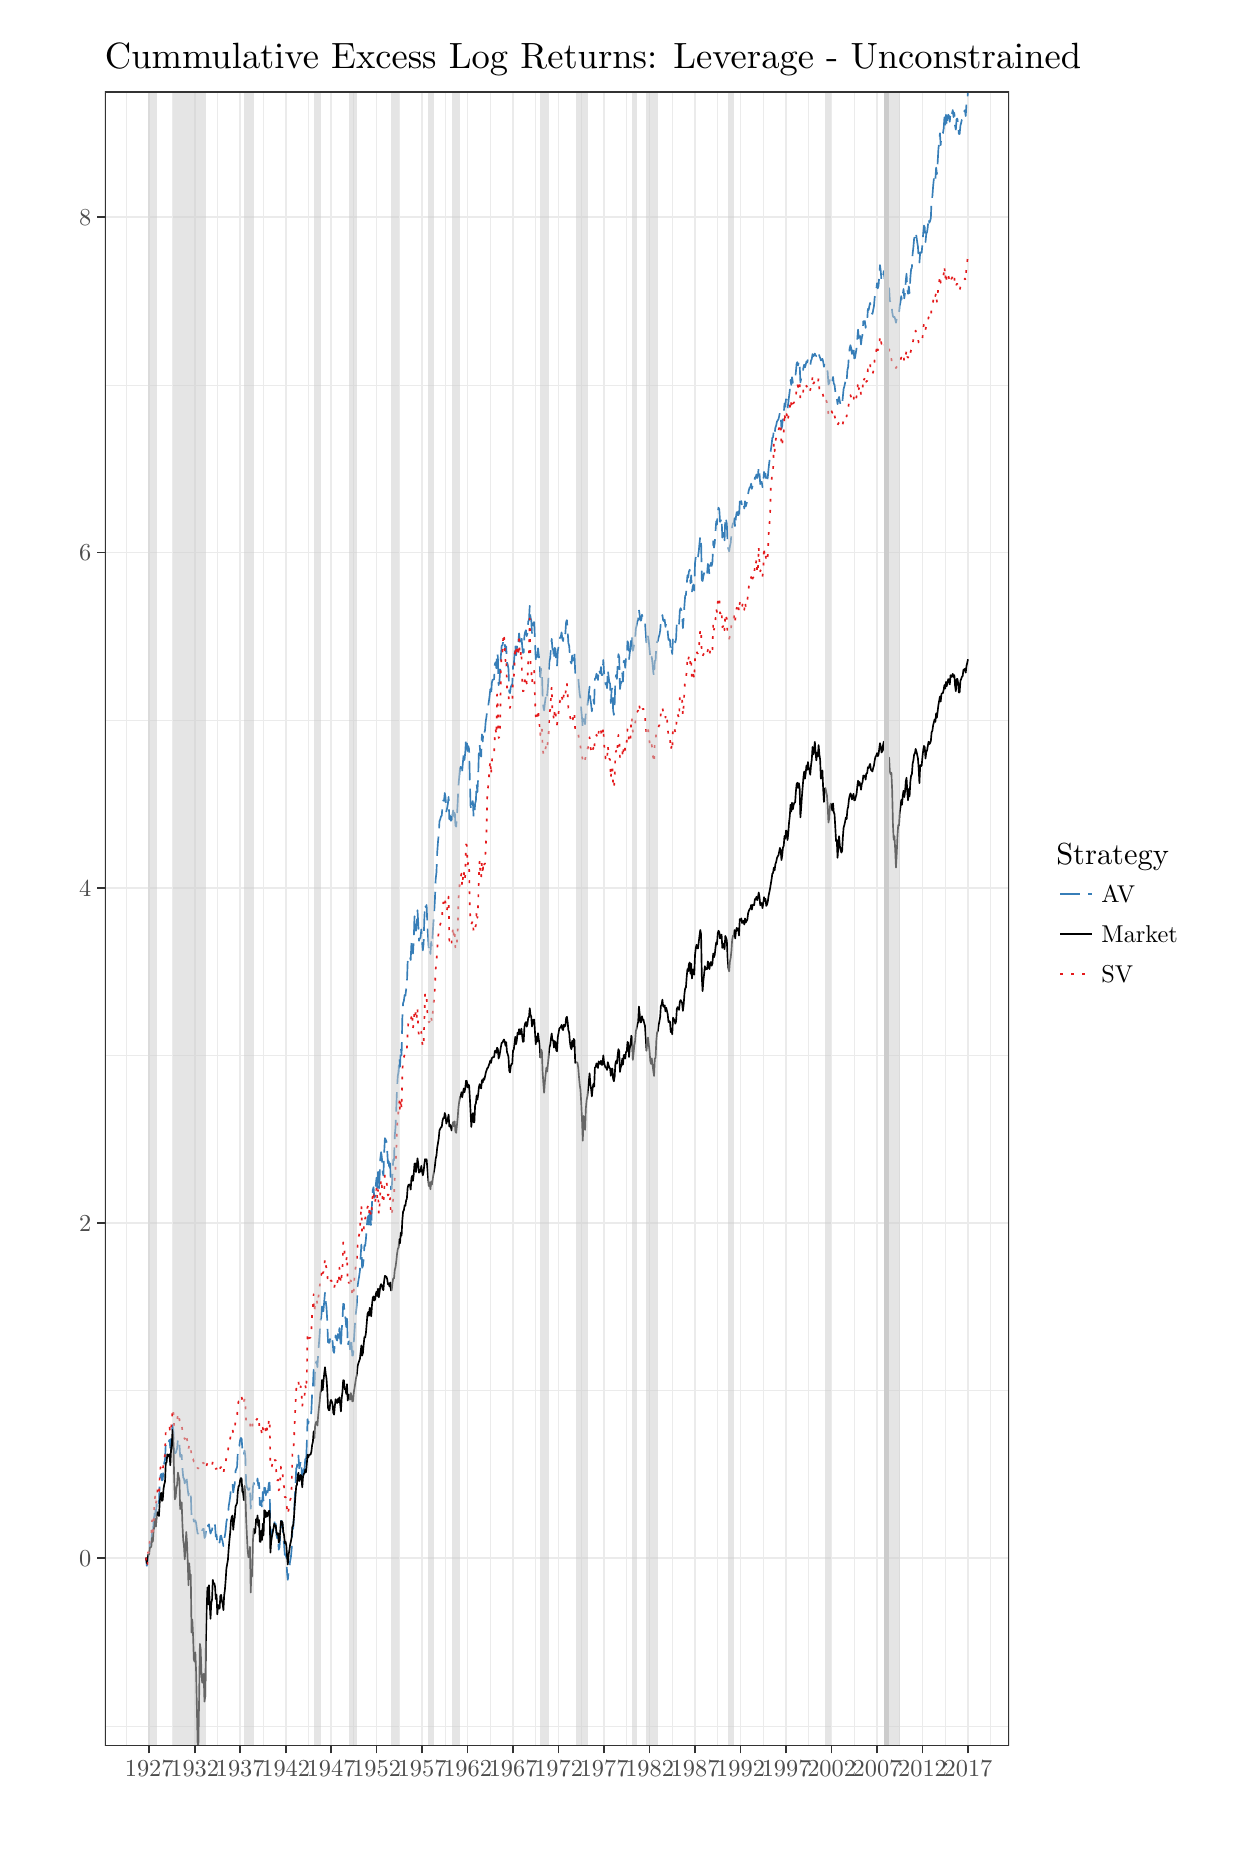
\begin{tikzpicture}[x=1pt,y=1pt]
\definecolor{fillColor}{RGB}{255,255,255}
\path[use as bounding box,fill=fillColor,fill opacity=0.00] (0,0) rectangle (426.79,650.43);
\begin{scope}
\path[clip] (  0.00,  0.00) rectangle (426.79,650.43);
\definecolor{drawColor}{RGB}{255,255,255}
\definecolor{fillColor}{RGB}{255,255,255}

\path[draw=drawColor,line width= 0.6pt,line join=round,line cap=round,fill=fillColor] (  0.00,  0.00) rectangle (426.79,650.43);
\end{scope}
\begin{scope}
\path[clip] ( 27.92, 29.59) rectangle (354.63,627.29);
\definecolor{fillColor}{RGB}{255,255,255}

\path[fill=fillColor] ( 27.92, 29.59) rectangle (354.63,627.29);
\definecolor{drawColor}{gray}{0.92}

\path[draw=drawColor,line width= 0.3pt,line join=round] ( 27.92, 36.76) --
	(354.63, 36.76);

\path[draw=drawColor,line width= 0.3pt,line join=round] ( 27.92,157.90) --
	(354.63,157.90);

\path[draw=drawColor,line width= 0.3pt,line join=round] ( 27.92,279.04) --
	(354.63,279.04);

\path[draw=drawColor,line width= 0.3pt,line join=round] ( 27.92,400.18) --
	(354.63,400.18);

\path[draw=drawColor,line width= 0.3pt,line join=round] ( 27.92,521.33) --
	(354.63,521.33);

\path[draw=drawColor,line width= 0.3pt,line join=round] ( 35.69, 29.59) --
	( 35.69,627.29);

\path[draw=drawColor,line width= 0.3pt,line join=round] ( 52.13, 29.59) --
	( 52.13,627.29);

\path[draw=drawColor,line width= 0.3pt,line join=round] ( 68.57, 29.59) --
	( 68.57,627.29);

\path[draw=drawColor,line width= 0.3pt,line join=round] ( 85.01, 29.59) --
	( 85.01,627.29);

\path[draw=drawColor,line width= 0.3pt,line join=round] (101.45, 29.59) --
	(101.45,627.29);

\path[draw=drawColor,line width= 0.3pt,line join=round] (117.88, 29.59) --
	(117.88,627.29);

\path[draw=drawColor,line width= 0.3pt,line join=round] (134.32, 29.59) --
	(134.32,627.29);

\path[draw=drawColor,line width= 0.3pt,line join=round] (150.77, 29.59) --
	(150.77,627.29);

\path[draw=drawColor,line width= 0.3pt,line join=round] (167.20, 29.59) --
	(167.20,627.29);

\path[draw=drawColor,line width= 0.3pt,line join=round] (183.64, 29.59) --
	(183.64,627.29);

\path[draw=drawColor,line width= 0.3pt,line join=round] (200.08, 29.59) --
	(200.08,627.29);

\path[draw=drawColor,line width= 0.3pt,line join=round] (216.52, 29.59) --
	(216.52,627.29);

\path[draw=drawColor,line width= 0.3pt,line join=round] (232.96, 29.59) --
	(232.96,627.29);

\path[draw=drawColor,line width= 0.3pt,line join=round] (249.39, 29.59) --
	(249.39,627.29);

\path[draw=drawColor,line width= 0.3pt,line join=round] (265.84, 29.59) --
	(265.84,627.29);

\path[draw=drawColor,line width= 0.3pt,line join=round] (282.28, 29.59) --
	(282.28,627.29);

\path[draw=drawColor,line width= 0.3pt,line join=round] (298.71, 29.59) --
	(298.71,627.29);

\path[draw=drawColor,line width= 0.3pt,line join=round] (315.15, 29.59) --
	(315.15,627.29);

\path[draw=drawColor,line width= 0.3pt,line join=round] (331.59, 29.59) --
	(331.59,627.29);

\path[draw=drawColor,line width= 0.3pt,line join=round] (348.03, 29.59) --
	(348.03,627.29);

\path[draw=drawColor,line width= 0.6pt,line join=round] ( 27.92, 97.33) --
	(354.63, 97.33);

\path[draw=drawColor,line width= 0.6pt,line join=round] ( 27.92,218.47) --
	(354.63,218.47);

\path[draw=drawColor,line width= 0.6pt,line join=round] ( 27.92,339.61) --
	(354.63,339.61);

\path[draw=drawColor,line width= 0.6pt,line join=round] ( 27.92,460.75) --
	(354.63,460.75);

\path[draw=drawColor,line width= 0.6pt,line join=round] ( 27.92,581.90) --
	(354.63,581.90);

\path[draw=drawColor,line width= 0.6pt,line join=round] ( 43.91, 29.59) --
	( 43.91,627.29);

\path[draw=drawColor,line width= 0.6pt,line join=round] ( 60.35, 29.59) --
	( 60.35,627.29);

\path[draw=drawColor,line width= 0.6pt,line join=round] ( 76.79, 29.59) --
	( 76.79,627.29);

\path[draw=drawColor,line width= 0.6pt,line join=round] ( 93.23, 29.59) --
	( 93.23,627.29);

\path[draw=drawColor,line width= 0.6pt,line join=round] (109.66, 29.59) --
	(109.66,627.29);

\path[draw=drawColor,line width= 0.6pt,line join=round] (126.10, 29.59) --
	(126.10,627.29);

\path[draw=drawColor,line width= 0.6pt,line join=round] (142.55, 29.59) --
	(142.55,627.29);

\path[draw=drawColor,line width= 0.6pt,line join=round] (158.98, 29.59) --
	(158.98,627.29);

\path[draw=drawColor,line width= 0.6pt,line join=round] (175.42, 29.59) --
	(175.42,627.29);

\path[draw=drawColor,line width= 0.6pt,line join=round] (191.86, 29.59) --
	(191.86,627.29);

\path[draw=drawColor,line width= 0.6pt,line join=round] (208.30, 29.59) --
	(208.30,627.29);

\path[draw=drawColor,line width= 0.6pt,line join=round] (224.74, 29.59) --
	(224.74,627.29);

\path[draw=drawColor,line width= 0.6pt,line join=round] (241.18, 29.59) --
	(241.18,627.29);

\path[draw=drawColor,line width= 0.6pt,line join=round] (257.61, 29.59) --
	(257.61,627.29);

\path[draw=drawColor,line width= 0.6pt,line join=round] (274.06, 29.59) --
	(274.06,627.29);

\path[draw=drawColor,line width= 0.6pt,line join=round] (290.50, 29.59) --
	(290.50,627.29);

\path[draw=drawColor,line width= 0.6pt,line join=round] (306.93, 29.59) --
	(306.93,627.29);

\path[draw=drawColor,line width= 0.6pt,line join=round] (323.37, 29.59) --
	(323.37,627.29);

\path[draw=drawColor,line width= 0.6pt,line join=round] (339.81, 29.59) --
	(339.81,627.29);
\definecolor{drawColor}{RGB}{55,126,184}

\path[draw=drawColor,line width= 0.6pt,dash pattern=on 7pt off 3pt ,line join=round] ( 42.78, 97.57) --
	( 43.05, 94.59) --
	( 43.32, 96.11) --
	( 43.60, 98.48) --
	( 43.87, 98.42) --
	( 44.15,102.56) --
	( 44.43,102.68) --
	( 44.68,103.01) --
	( 44.96,107.53) --
	( 45.23,105.48) --
	( 45.51,111.01) --
	( 45.78,112.72) --
	( 46.06,115.94) --
	( 46.34,112.64) --
	( 46.61,117.38) --
	( 46.89,119.07) --
	( 47.16,118.63) --
	( 47.44,117.17) --
	( 47.72,125.04) --
	( 47.98,127.09) --
	( 48.26,127.84) --
	( 48.53,125.49) --
	( 48.81,125.71) --
	( 49.08,130.18) --
	( 49.36,131.89) --
	( 49.63,132.87) --
	( 49.90,138.80) --
	( 50.18,138.86) --
	( 50.45,140.21) --
	( 50.73,140.17) --
	( 51.01,139.66) --
	( 51.26,140.11) --
	( 51.54,137.20) --
	( 51.81,140.50) --
	( 52.09,142.20) --
	( 52.36,145.46) --
	( 52.64,143.65) --
	( 52.92,135.79) --
	( 53.19,135.30) --
	( 53.47,135.37) --
	( 53.74,136.22) --
	( 54.02,137.15) --
	( 54.30,140.57) --
	( 54.55,139.60) --
	( 54.83,138.82) --
	( 55.10,134.01) --
	( 55.38,134.63) --
	( 55.65,134.66) --
	( 55.93,129.64) --
	( 56.21,126.55) --
	( 56.48,126.09) --
	( 56.75,124.42) --
	( 57.02,125.43) --
	( 57.30,127.39) --
	( 57.58,124.84) --
	( 57.83,122.24) --
	( 58.11,120.05) --
	( 58.38,121.80) --
	( 58.66,121.14) --
	( 58.93,121.20) --
	( 59.21,112.46) --
	( 59.49,113.21) --
	( 59.76,112.74) --
	( 60.04,110.65) --
	( 60.31,110.57) --
	( 60.59,111.03) --
	( 60.87,110.06) --
	( 61.13,108.12) --
	( 61.41,106.31) --
	( 61.68,106.27) --
	( 61.96,107.69) --
	( 62.23,108.33) --
	( 62.51,108.18) --
	( 62.79,107.75) --
	( 63.06,107.48) --
	( 63.33,107.90) --
	( 63.60,107.99) --
	( 63.88,104.68) --
	( 64.16,105.14) --
	( 64.41,107.10) --
	( 64.69,108.51) --
	( 64.96,109.81) --
	( 65.24,108.88) --
	( 65.51,109.62) --
	( 65.79,107.69) --
	( 66.07,106.31) --
	( 66.34,107.20) --
	( 66.62,107.51) --
	( 66.89,110.23) --
	( 67.17,109.67) --
	( 67.45,109.78) --
	( 67.70,109.21) --
	( 67.98,105.23) --
	( 68.25,105.85) --
	( 68.53,102.58) --
	( 68.80,103.64) --
	( 69.08,103.58) --
	( 69.36,102.99) --
	( 69.63,105.39) --
	( 69.91,105.53) --
	( 70.18,104.31) --
	( 70.45,103.38) --
	( 70.73,101.73) --
	( 70.99,104.25) --
	( 71.26,105.48) --
	( 71.53,107.40) --
	( 71.81,110.42) --
	( 72.08,111.76) --
	( 72.36,112.57) --
	( 72.64,116.13) --
	( 72.91,117.81) --
	( 73.19,119.69) --
	( 73.46,122.71) --
	( 73.74,123.84) --
	( 74.02,124.26) --
	( 74.28,121.15) --
	( 74.56,123.01) --
	( 74.83,124.20) --
	( 75.11,128.89) --
	( 75.38,129.60) --
	( 75.66,130.34) --
	( 75.94,135.88) --
	( 76.21,137.91) --
	( 76.49,138.02) --
	( 76.76,140.03) --
	( 77.03,140.82) --
	( 77.31,140.61) --
	( 77.57,136.91) --
	( 77.84,136.65) --
	( 78.11,134.52) --
	( 78.39,136.28) --
	( 78.66,134.14) --
	( 78.94,124.46) --
	( 79.22,122.97) --
	( 79.49,122.39) --
	( 79.77,121.99) --
	( 80.04,122.17) --
	( 80.32,123.46) --
	( 80.60,115.27) --
	( 80.85,117.89) --
	( 81.13,117.32) --
	( 81.40,123.09) --
	( 81.68,124.60) --
	( 81.95,123.82) --
	( 82.23,123.93) --
	( 82.51,125.04) --
	( 82.78,124.39) --
	( 83.06,126.19) --
	( 83.33,123.63) --
	( 83.61,124.64) --
	( 83.88,116.62) --
	( 84.14,116.56) --
	( 84.42,118.15) --
	( 84.69,115.21) --
	( 84.96,121.30) --
	( 85.23,117.87) --
	( 85.51,122.81) --
	( 85.79,122.77) --
	( 86.06,120.05) --
	( 86.34,122.78) --
	( 86.61,120.76) --
	( 86.89,122.07) --
	( 87.17,124.59) --
	( 87.43,124.67) --
	( 87.71,104.92) --
	( 87.98,105.70) --
	( 88.26,106.37) --
	( 88.53,108.11) --
	( 88.81,109.25) --
	( 89.09,110.76) --
	( 89.36,109.58) --
	( 89.64,109.81) --
	( 89.91,105.63) --
	( 90.19,104.55) --
	( 90.46,105.16) --
	( 90.72,100.45) --
	( 91.00,101.33) --
	( 91.27,105.55) --
	( 91.54,110.83) --
	( 91.81,110.74) --
	( 92.09,109.79) --
	( 92.37,104.39) --
	( 92.64,102.64) --
	( 92.92, 98.54) --
	( 93.19, 98.75) --
	( 93.47, 97.58) --
	( 93.75, 91.88) --
	( 94.00, 89.56) --
	( 94.28, 92.48) --
	( 94.55, 94.00) --
	( 94.83, 96.37) --
	( 95.10, 97.65) --
	( 95.38,100.53) --
	( 95.66,107.97) --
	( 95.93,108.03) --
	( 96.21,112.61) --
	( 96.48,118.20) --
	( 96.76,123.77) --
	( 97.04,129.75) --
	( 97.29,130.25) --
	( 97.57,133.30) --
	( 97.84,134.48) --
	( 98.12,129.84) --
	( 98.39,130.73) --
	( 98.67,132.62) --
	( 98.94,131.11) --
	( 99.21,123.76) --
	( 99.49,127.88) --
	( 99.76,129.41) --
	(100.04,129.81) --
	(100.32,133.25) --
	(100.58,131.24) --
	(100.86,138.64) --
	(101.13,147.61) --
	(101.41,145.99) --
	(101.68,147.59) --
	(101.96,147.61) --
	(102.24,147.81) --
	(102.51,150.51) --
	(102.79,156.99) --
	(103.06,159.09) --
	(103.34,165.49) --
	(103.62,159.65) --
	(103.87,166.12) --
	(104.15,168.05) --
	(104.42,168.51) --
	(104.70,166.39) --
	(104.97,171.39) --
	(105.25,174.86) --
	(105.52,178.58) --
	(105.79,183.33) --
	(106.07,184.23) --
	(106.34,188.31) --
	(106.62,184.86) --
	(106.90,187.16) --
	(107.15,190.08) --
	(107.43,193.28) --
	(107.70,190.19) --
	(107.98,187.99) --
	(108.25,183.18) --
	(108.53,175.45) --
	(108.81,175.22) --
	(109.08,175.23) --
	(109.36,177.37) --
	(109.63,177.87) --
	(109.91,177.14) --
	(110.19,175.61) --
	(110.44,172.26) --
	(110.72,171.58) --
	(110.99,174.77) --
	(111.27,177.89) --
	(111.54,176.57) --
	(111.82,176.02) --
	(112.10,178.39) --
	(112.37,176.42) --
	(112.64,180.53) --
	(112.91,177.20) --
	(113.19,173.28) --
	(113.47,180.09) --
	(113.73,182.71) --
	(114.01,189.29) --
	(114.28,189.20) --
	(114.56,184.24) --
	(114.83,184.44) --
	(115.11,180.93) --
	(115.39,185.49) --
	(115.66,174.19) --
	(115.94,175.54) --
	(116.21,175.79) --
	(116.49,172.81) --
	(116.77,176.93) --
	(117.02,174.92) --
	(117.30,170.54) --
	(117.57,170.71) --
	(117.85,175.52) --
	(118.12,179.91) --
	(118.40,183.75) --
	(118.68,186.70) --
	(118.95,189.08) --
	(119.22,195.60) --
	(119.49,197.58) --
	(119.77,199.17) --
	(120.05,201.19) --
	(120.30,206.06) --
	(120.58,210.72) --
	(120.85,202.30) --
	(121.13,202.91) --
	(121.40,205.39) --
	(121.68,210.49) --
	(121.96,210.24) --
	(122.23,212.75) --
	(122.51,216.63) --
	(122.78,220.04) --
	(123.06,221.07) --
	(123.34,217.88) --
	(123.59,222.92) --
	(123.87,219.84) --
	(124.14,217.00) --
	(124.42,225.56) --
	(124.69,230.37) --
	(124.97,231.42) --
	(125.25,227.63) --
	(125.52,228.04) --
	(125.80,232.17) --
	(126.07,234.87) --
	(126.34,231.14) --
	(126.62,236.99) --
	(126.88,230.34) --
	(127.16,234.87) --
	(127.43,241.73) --
	(127.71,244.09) --
	(127.98,242.33) --
	(128.26,236.97) --
	(128.54,235.65) --
	(128.81,243.70) --
	(129.09,249.14) --
	(129.36,248.63) --
	(129.64,247.91) --
	(129.92,244.64) --
	(130.17,240.13) --
	(130.45,240.79) --
	(130.72,237.07) --
	(131.00,240.06) --
	(131.27,230.63) --
	(131.55,230.93) --
	(131.83,236.52) --
	(132.10,241.35) --
	(132.38,241.22) --
	(132.65,250.14) --
	(132.92,253.11) --
	(133.20,260.16) --
	(133.46,266.95) --
	(133.73,271.47) --
	(134.00,273.25) --
	(134.28,278.19) --
	(134.55,274.98) --
	(134.83,281.84) --
	(135.11,279.14) --
	(135.38,292.53) --
	(135.66,298.02) --
	(135.93,298.70) --
	(136.21,300.85) --
	(136.49,300.62) --
	(136.74,302.79) --
	(137.02,304.34) --
	(137.29,312.48) --
	(137.57,314.90) --
	(137.84,315.16) --
	(138.12,314.77) --
	(138.40,313.53) --
	(138.67,319.56) --
	(138.95,320.89) --
	(139.22,315.85) --
	(139.50,320.50) --
	(139.77,329.18) --
	(140.04,329.55) --
	(140.31,324.06) --
	(140.58,327.12) --
	(140.86,331.48) --
	(141.13,326.87) --
	(141.41,320.47) --
	(141.69,321.31) --
	(141.96,321.60) --
	(142.24,324.58) --
	(142.51,320.04) --
	(142.79,317.02) --
	(143.07,319.59) --
	(143.32,328.23) --
	(143.60,333.57) --
	(143.87,332.57) --
	(144.15,333.40) --
	(144.42,326.50) --
	(144.70,321.40) --
	(144.98,316.82) --
	(145.25,317.70) --
	(145.53,315.71) --
	(145.80,320.10) --
	(146.08,318.35) --
	(146.35,322.86) --
	(146.61,327.40) --
	(146.89,330.65) --
	(147.16,335.49) --
	(147.43,342.79) --
	(147.71,345.17) --
	(147.98,352.27) --
	(148.26,356.13) --
	(148.53,359.01) --
	(148.81,363.71) --
	(149.08,364.39) --
	(149.36,365.41) --
	(149.64,365.72) --
	(149.89,369.43) --
	(150.17,371.21) --
	(150.44,371.06) --
	(150.72,373.85) --
	(150.99,372.36) --
	(151.27,367.19) --
	(151.55,368.31) --
	(151.82,369.85) --
	(152.10,372.47) --
	(152.37,364.32) --
	(152.65,365.64) --
	(152.93,364.08) --
	(153.19,362.35) --
	(153.47,365.75) --
	(153.74,367.59) --
	(154.02,365.59) --
	(154.29,368.34) --
	(154.56,362.22) --
	(154.84,361.72) --
	(155.11,365.60) --
	(155.39,370.60) --
	(155.66,376.49) --
	(155.94,379.69) --
	(156.22,382.82) --
	(156.47,383.22) --
	(156.75,384.98) --
	(157.02,381.95) --
	(157.30,385.26) --
	(157.57,388.27) --
	(157.85,385.80) --
	(158.13,388.68) --
	(158.40,393.61) --
	(158.68,393.48) --
	(158.95,389.06) --
	(159.23,390.79) --
	(159.51,389.69) --
	(159.76,378.99) --
	(160.04,369.26) --
	(160.31,367.54) --
	(160.59,369.47) --
	(160.86,370.97) --
	(161.14,365.20) --
	(161.41,365.18) --
	(161.68,370.12) --
	(161.96,371.02) --
	(162.23,377.27) --
	(162.51,374.18) --
	(162.79,379.93) --
	(163.04,388.61) --
	(163.32,391.29) --
	(163.59,387.81) --
	(163.87,387.01) --
	(164.14,395.06) --
	(164.42,392.49) --
	(164.70,396.47) --
	(164.97,395.54) --
	(165.25,396.47) --
	(165.52,399.80) --
	(165.80,401.55) --
	(166.08,404.44) --
	(166.34,404.79) --
	(166.62,406.77) --
	(166.89,408.74) --
	(167.17,411.40) --
	(167.44,408.83) --
	(167.72,413.67) --
	(167.99,414.79) --
	(168.26,414.84) --
	(168.54,414.98) --
	(168.81,420.39) --
	(169.09,421.14) --
	(169.37,418.93) --
	(169.62,424.65) --
	(169.90,423.09) --
	(170.17,412.84) --
	(170.45,414.01) --
	(170.72,418.15) --
	(171.00,423.53) --
	(171.28,427.19) --
	(171.55,427.18) --
	(171.83,428.60) --
	(172.10,429.48) --
	(172.38,428.04) --
	(172.66,425.07) --
	(172.91,426.80) --
	(173.19,421.07) --
	(173.46,420.27) --
	(173.74,418.68) --
	(174.01,410.46) --
	(174.29,409.97) --
	(174.57,412.22) --
	(174.84,412.81) --
	(175.11,412.96) --
	(175.38,419.65) --
	(175.66,420.19) --
	(175.94,424.43) --
	(176.19,427.71) --
	(176.47,423.59) --
	(176.74,425.66) --
	(177.02,429.13) --
	(177.29,428.34) --
	(177.57,431.56) --
	(177.85,428.48) --
	(178.12,428.90) --
	(178.40,430.99) --
	(178.67,427.24) --
	(178.95,424.55) --
	(179.23,424.64) --
	(179.49,430.70) --
	(179.77,432.08) --
	(180.04,432.69) --
	(180.32,430.58) --
	(180.59,431.64) --
	(180.87,435.84) --
	(181.15,436.33) --
	(181.42,441.50) --
	(181.69,437.32) --
	(181.96,436.30) --
	(182.24,431.31) --
	(182.52,433.99) --
	(182.77,435.53) --
	(183.05,435.57) --
	(183.32,428.31) --
	(183.60,422.15) --
	(183.87,424.56) --
	(184.15,422.45) --
	(184.43,426.17) --
	(184.70,423.61) --
	(184.98,421.05) --
	(185.25,415.75) --
	(185.53,418.79) --
	(185.81,418.17) --
	(186.06,409.41) --
	(186.34,404.98) --
	(186.61,403.72) --
	(186.89,406.38) --
	(187.16,408.36) --
	(187.44,410.57) --
	(187.72,409.05) --
	(187.99,412.27) --
	(188.27,417.11) --
	(188.54,421.47) --
	(188.81,422.58) --
	(189.09,426.65) --
	(189.35,429.57) --
	(189.62,425.86) --
	(189.89,425.90) --
	(190.17,422.09) --
	(190.44,426.34) --
	(190.72,425.87) --
	(191.00,420.19) --
	(191.27,419.70) --
	(191.55,424.99) --
	(191.82,426.76) --
	(192.10,429.42) --
	(192.38,430.04) --
	(192.64,430.33) --
	(192.92,431.91) --
	(193.19,429.59) --
	(193.47,428.76) --
	(193.74,431.81) --
	(194.02,430.96) --
	(194.30,431.65) --
	(194.57,435.68) --
	(194.85,436.35) --
	(195.12,432.34) --
	(195.39,427.98) --
	(195.67,427.09) --
	(195.93,423.23) --
	(196.20,421.30) --
	(196.47,420.67) --
	(196.75,423.57) --
	(197.02,421.68) --
	(197.30,424.97) --
	(197.58,424.50) --
	(197.85,417.24) --
	(198.13,417.41) --
	(198.40,417.38) --
	(198.68,417.25) --
	(198.96,415.54) --
	(199.21,412.37) --
	(199.49,409.47) --
	(199.76,408.09) --
	(200.04,403.88) --
	(200.31,400.98) --
	(200.59,397.31) --
	(200.87,400.63) --
	(201.14,399.81) --
	(201.42,398.72) --
	(201.69,403.07) --
	(201.97,404.51) --
	(202.24,405.56) --
	(202.50,407.52) --
	(202.78,409.84) --
	(203.05,412.30) --
	(203.32,407.90) --
	(203.60,405.86) --
	(203.87,403.39) --
	(204.15,406.13) --
	(204.42,407.57) --
	(204.70,406.04) --
	(204.97,415.20) --
	(205.25,415.36) --
	(205.53,416.98) --
	(205.79,415.98) --
	(206.07,414.72) --
	(206.34,418.81) --
	(206.62,417.84) --
	(206.89,417.12) --
	(207.17,419.43) --
	(207.45,416.46) --
	(207.72,416.56) --
	(208.00,421.94) --
	(208.27,417.35) --
	(208.55,415.05) --
	(208.82,413.17) --
	(209.08,413.35) --
	(209.36,411.75) --
	(209.63,418.40) --
	(209.91,416.06) --
	(210.18,413.79) --
	(210.45,413.45) --
	(210.73,406.34) --
	(211.00,411.28) --
	(211.28,411.60) --
	(211.55,403.77) --
	(211.83,402.08) --
	(212.11,406.28) --
	(212.36,414.98) --
	(212.64,416.53) --
	(212.91,415.09) --
	(213.19,420.12) --
	(213.46,424.03) --
	(213.74,423.06) --
	(214.02,411.44) --
	(214.29,413.32) --
	(214.57,413.91) --
	(214.84,417.39) --
	(215.12,414.14) --
	(215.40,421.57) --
	(215.65,421.70) --
	(215.93,419.09) --
	(216.20,422.62) --
	(216.48,423.28) --
	(216.75,428.69) --
	(217.03,428.04) --
	(217.30,422.04) --
	(217.57,424.69) --
	(217.85,426.01) --
	(218.12,430.99) --
	(218.40,430.67) --
	(218.68,425.28) --
	(218.94,426.38) --
	(219.22,428.22) --
	(219.49,429.61) --
	(219.77,433.34) --
	(220.04,434.39) --
	(220.32,435.88) --
	(220.60,436.43) --
	(220.87,440.13) --
	(221.15,438.02) --
	(221.42,436.14) --
	(221.70,436.27) --
	(221.98,438.31) --
	(222.23,437.40) --
	(222.51,437.47) --
	(222.78,436.28) --
	(223.06,435.68) --
	(223.33,431.79) --
	(223.61,427.74) --
	(223.88,429.39) --
	(224.15,430.52) --
	(224.43,428.74) --
	(224.70,425.87) --
	(224.98,422.83) --
	(225.26,421.70) --
	(225.51,423.07) --
	(225.79,420.64) --
	(226.06,417.63) --
	(226.34,415.96) --
	(226.61,421.66) --
	(226.89,421.83) --
	(227.17,427.32) --
	(227.44,428.48) --
	(227.72,428.76) --
	(227.99,430.13) --
	(228.27,430.96) --
	(228.55,432.49) --
	(228.80,435.84) --
	(229.08,436.28) --
	(229.35,438.19) --
	(229.63,436.21) --
	(229.90,436.02) --
	(230.18,436.52) --
	(230.46,433.90) --
	(230.73,435.22) --
	(231.00,433.89) --
	(231.27,432.28) --
	(231.55,429.17) --
	(231.83,429.46) --
	(232.09,429.19) --
	(232.37,424.76) --
	(232.64,425.84) --
	(232.92,424.10) --
	(233.19,430.63) --
	(233.47,430.28) --
	(233.75,429.58) --
	(234.02,428.27) --
	(234.30,429.59) --
	(234.57,435.69) --
	(234.85,436.40) --
	(235.13,435.66) --
	(235.38,435.00) --
	(235.66,439.84) --
	(235.93,440.66) --
	(236.21,439.98) --
	(236.48,439.13) --
	(236.76,433.42) --
	(237.04,437.19) --
	(237.31,441.50) --
	(237.58,445.12) --
	(237.85,445.38) --
	(238.13,449.15) --
	(238.41,452.50) --
	(238.66,451.68) --
	(238.94,453.89) --
	(239.21,454.55) --
	(239.49,449.65) --
	(239.76,452.53) --
	(240.04,446.67) --
	(240.32,448.49) --
	(240.59,449.22) --
	(240.87,447.03) --
	(241.14,456.91) --
	(241.42,459.26) --
	(241.70,460.56) --
	(241.95,459.28) --
	(242.23,459.29) --
	(242.50,461.21) --
	(242.78,464.28) --
	(243.05,466.72) --
	(243.33,465.06) --
	(243.61,450.82) --
	(243.88,450.48) --
	(244.16,452.21) --
	(244.43,453.33) --
	(244.70,454.49) --
	(244.98,453.25) --
	(245.24,453.62) --
	(245.52,453.39) --
	(245.79,456.64) --
	(246.07,455.78) --
	(246.34,452.87) --
	(246.62,455.91) --
	(246.90,457.07) --
	(247.17,455.92) --
	(247.45,457.40) --
	(247.72,464.89) --
	(248.00,462.54) --
	(248.28,464.27) --
	(248.53,468.17) --
	(248.81,472.07) --
	(249.08,470.86) --
	(249.36,475.56) --
	(249.63,476.99) --
	(249.91,476.31) --
	(250.19,471.86) --
	(250.46,472.26) --
	(250.74,473.36) --
	(251.01,466.14) --
	(251.28,466.65) --
	(251.56,468.34) --
	(251.82,465.15) --
	(252.09,473.63) --
	(252.36,472.59) --
	(252.64,471.18) --
	(252.91,464.09) --
	(253.19,462.23) --
	(253.47,461.18) --
	(253.74,463.00) --
	(254.02,464.19) --
	(254.29,467.28) --
	(254.57,470.17) --
	(254.85,471.30) --
	(255.10,471.21) --
	(255.38,473.17) --
	(255.65,469.77) --
	(255.93,473.58) --
	(256.20,475.34) --
	(256.48,474.30) --
	(256.76,475.62) --
	(257.03,472.82) --
	(257.31,479.21) --
	(257.58,478.92) --
	(257.86,479.38) --
	(258.13,477.47) --
	(258.40,478.51) --
	(258.67,478.67) --
	(258.94,476.68) --
	(259.22,479.30) --
	(259.49,477.44) --
	(259.77,478.50) --
	(260.05,479.23) --
	(260.32,481.93) --
	(260.60,483.33) --
	(260.87,484.23) --
	(261.15,484.43) --
	(261.43,485.68) --
	(261.68,483.75) --
	(261.96,484.98) --
	(262.23,485.22) --
	(262.51,485.00) --
	(262.78,487.89) --
	(263.06,487.75) --
	(263.34,488.98) --
	(263.61,487.66) --
	(263.89,488.82) --
	(264.16,491.61) --
	(264.44,489.51) --
	(264.71,485.48) --
	(264.97,485.97) --
	(265.25,486.32) --
	(265.52,484.38) --
	(265.80,486.45) --
	(266.07,489.91) --
	(266.34,488.25) --
	(266.62,489.31) --
	(266.89,485.93) --
	(267.17,486.65) --
	(267.44,488.04) --
	(267.72,491.09) --
	(268.00,493.48) --
	(268.25,495.26) --
	(268.53,497.73) --
	(268.80,499.63) --
	(269.08,502.17) --
	(269.35,502.46) --
	(269.63,505.13) --
	(269.91,503.83) --
	(270.18,505.93) --
	(270.46,506.59) --
	(270.73,508.03) --
	(271.01,508.52) --
	(271.29,508.95) --
	(271.55,510.02) --
	(271.83,511.38) --
	(272.10,510.46) --
	(272.38,505.42) --
	(272.65,506.59) --
	(272.92,509.96) --
	(273.20,510.73) --
	(273.47,514.64) --
	(273.75,513.46) --
	(274.02,516.16) --
	(274.30,515.86) --
	(274.58,512.87) --
	(274.83,514.69) --
	(275.11,517.10) --
	(275.38,519.27) --
	(275.66,523.16) --
	(275.93,521.34) --
	(276.21,524.10) --
	(276.49,522.10) --
	(276.76,522.69) --
	(277.04,523.34) --
	(277.31,523.37) --
	(277.59,526.05) --
	(277.87,529.16) --
	(278.12,529.55) --
	(278.40,528.38) --
	(278.67,530.09) --
	(278.95,528.86) --
	(279.22,522.27) --
	(279.50,523.53) --
	(279.77,524.64) --
	(280.04,525.49) --
	(280.32,527.67) --
	(280.59,528.64) --
	(280.87,527.67) --
	(281.15,528.62) --
	(281.40,529.84) --
	(281.68,529.42) --
	(281.95,530.66) --
	(282.23,529.71) --
	(282.50,529.16) --
	(282.78,528.34) --
	(283.06,530.07) --
	(283.33,530.72) --
	(283.61,532.47) --
	(283.88,531.67) --
	(284.16,531.97) --
	(284.44,532.66) --
	(284.70,532.05) --
	(284.98,531.71) --
	(285.25,532.32) --
	(285.53,531.98) --
	(285.80,533.10) --
	(286.08,531.75) --
	(286.35,531.16) --
	(286.62,530.17) --
	(286.90,530.38) --
	(287.17,530.76) --
	(287.45,529.74) --
	(287.73,527.89) --
	(287.98,528.96) --
	(288.26,529.04) --
	(288.53,528.36) --
	(288.81,527.57) --
	(289.08,525.77) --
	(289.36,521.50) --
	(289.64,521.98) --
	(289.91,523.63) --
	(290.19,524.25) --
	(290.46,523.45) --
	(290.74,522.54) --
	(291.02,524.22) --
	(291.27,521.85) --
	(291.55,521.39) --
	(291.82,519.11) --
	(292.10,516.52) --
	(292.37,516.59) --
	(292.65,514.39) --
	(292.93,516.20) --
	(293.20,516.98) --
	(293.47,515.42) --
	(293.74,514.16) --
	(294.02,513.60) --
	(294.30,514.15) --
	(294.55,516.89) --
	(294.83,519.90) --
	(295.10,520.75) --
	(295.38,522.12) --
	(295.65,523.49) --
	(295.93,522.56) --
	(296.21,526.74) --
	(296.48,527.84) --
	(296.76,532.28) --
	(297.03,534.64) --
	(297.31,535.68) --
	(297.59,534.48) --
	(297.85,532.53) --
	(298.13,533.48) --
	(298.40,535.45) --
	(298.68,530.91) --
	(298.95,531.07) --
	(299.23,532.82) --
	(299.51,534.51) --
	(299.78,537.92) --
	(300.05,541.30) --
	(300.32,538.26) --
	(300.60,540.40) --
	(300.88,538.45) --
	(301.13,535.96) --
	(301.41,538.42) --
	(301.68,539.50) --
	(301.96,544.39) --
	(302.23,543.52) --
	(302.51,544.44) --
	(302.79,541.95) --
	(303.06,544.08) --
	(303.34,544.15) --
	(303.61,548.78) --
	(303.89,548.41) --
	(304.17,549.98) --
	(304.42,550.98) --
	(304.70,547.65) --
	(304.97,547.37) --
	(305.25,546.99) --
	(305.52,548.37) --
	(305.80,549.85) --
	(306.08,553.10) --
	(306.35,554.88) --
	(306.63,555.59) --
	(306.90,558.05) --
	(307.17,556.22) --
	(307.45,557.08) --
	(307.71,560.55) --
	(307.98,564.62) --
	(308.25,562.54) --
	(308.53,558.90) --
	(308.80,559.38) --
	(309.08,560.65) --
	(309.36,562.47) --
	(309.63,559.65) --
	(309.91,559.44) --
	(310.18,555.46) --
	(310.46,554.81) --
	(310.74,554.33) --
	(311.00,555.51) --
	(311.28,556.31) --
	(311.55,551.76) --
	(311.83,551.12) --
	(312.10,551.26) --
	(312.38,547.78) --
	(312.66,546.13) --
	(312.93,545.79) --
	(313.21,545.92) --
	(313.48,545.09) --
	(313.75,543.80) --
	(314.03,545.22) --
	(314.29,546.16) --
	(314.56,547.19) --
	(314.84,547.13) --
	(315.11,550.02) --
	(315.38,551.15) --
	(315.66,553.42) --
	(315.94,551.80) --
	(316.21,554.01) --
	(316.49,556.00) --
	(316.76,552.59) --
	(317.04,554.84) --
	(317.32,559.15) --
	(317.57,561.51) --
	(317.85,555.87) --
	(318.12,554.25) --
	(318.40,556.95) --
	(318.67,554.47) --
	(318.95,560.05) --
	(319.23,563.20) --
	(319.50,563.63) --
	(319.78,568.70) --
	(320.05,571.11) --
	(320.33,574.37) --
	(320.60,574.66) --
	(320.86,576.62) --
	(321.14,574.97) --
	(321.41,573.08) --
	(321.69,571.37) --
	(321.96,566.86) --
	(322.23,565.55) --
	(322.51,569.22) --
	(322.78,569.05) --
	(323.06,569.16) --
	(323.33,572.65) --
	(323.61,576.24) --
	(323.89,578.91) --
	(324.15,578.22) --
	(324.43,572.93) --
	(324.70,575.92) --
	(324.98,576.52) --
	(325.25,578.39) --
	(325.53,581.70) --
	(325.81,579.95) --
	(326.08,580.57) --
	(326.36,581.62) --
	(326.63,588.60) --
	(326.91,589.41) --
	(327.19,593.24) --
	(327.44,595.68) --
	(327.72,596.99) --
	(327.99,595.50) --
	(328.27,599.88) --
	(328.54,597.48) --
	(328.81,601.54) --
	(329.09,606.64) --
	(329.36,608.81) --
	(329.64,612.27) --
	(329.91,607.97) --
	(330.19,611.63) --
	(330.47,612.10) --
	(330.72,612.30) --
	(331.00,613.96) --
	(331.27,618.04) --
	(331.55,614.52) --
	(331.82,618.93) --
	(332.10,614.77) --
	(332.38,617.81) --
	(332.65,618.97) --
	(332.93,618.49) --
	(333.20,616.43) --
	(333.48,619.92) --
	(333.76,618.82) --
	(334.01,619.55) --
	(334.29,620.66) --
	(334.56,618.10) --
	(334.84,619.69) --
	(335.11,615.00) --
	(335.39,613.59) --
	(335.66,617.39) --
	(335.93,617.54) --
	(336.21,615.60) --
	(336.48,611.99) --
	(336.76,612.01) --
	(337.04,615.01) --
	(337.30,616.04) --
	(337.58,617.19) --
	(337.85,617.50) --
	(338.13,619.82) --
	(338.40,620.16) --
	(338.68,620.59) --
	(338.96,618.46) --
	(339.23,623.12) --
	(339.51,624.25) --
	(339.78,627.29);
\definecolor{drawColor}{RGB}{0,0,0}

\path[draw=drawColor,line width= 0.6pt,line join=round] ( 42.78, 97.55) --
	( 43.05, 95.61) --
	( 43.32, 97.18) --
	( 43.60, 98.73) --
	( 43.87, 98.69) --
	( 44.15,101.21) --
	( 44.43,101.28) --
	( 44.68,101.56) --
	( 44.96,104.78) --
	( 45.23,103.34) --
	( 45.51,107.55) --
	( 45.78,108.74) --
	( 46.06,111.51) --
	( 46.34,108.82) --
	( 46.61,112.71) --
	( 46.89,113.98) --
	( 47.16,113.65) --
	( 47.44,112.63) --
	( 47.72,117.73) --
	( 47.98,120.13) --
	( 48.26,121.01) --
	( 48.53,118.08) --
	( 48.81,118.45) --
	( 49.08,122.37) --
	( 49.36,124.06) --
	( 49.63,125.02) --
	( 49.90,131.80) --
	( 50.18,131.89) --
	( 50.45,134.84) --
	( 50.73,134.78) --
	( 51.01,134.10) --
	( 51.26,134.91) --
	( 51.54,130.96) --
	( 51.81,136.60) --
	( 52.09,139.06) --
	( 52.36,143.71) --
	( 52.64,140.37) --
	( 52.92,126.86) --
	( 53.19,118.65) --
	( 53.47,119.35) --
	( 53.74,122.57) --
	( 54.02,124.03) --
	( 54.30,128.30) --
	( 54.55,126.87) --
	( 54.83,125.80) --
	( 55.10,115.11) --
	( 55.38,117.45) --
	( 55.65,117.50) --
	( 55.93,109.31) --
	( 56.21,103.77) --
	( 56.48,101.91) --
	( 56.75, 96.96) --
	( 57.02,100.62) --
	( 57.30,106.84) --
	( 57.58,102.82) --
	( 57.83, 96.40) --
	( 58.11, 87.62) --
	( 58.38, 95.52) --
	( 58.66, 91.30) --
	( 58.93, 91.44) --
	( 59.21, 70.51) --
	( 59.49, 75.24) --
	( 59.76, 69.62) --
	( 60.04, 60.77) --
	( 60.31, 60.03) --
	( 60.59, 63.35) --
	( 60.87, 56.11) --
	( 61.13, 44.00) --
	( 61.41, 29.91) --
	( 61.68, 29.59) --
	( 61.96, 47.31) --
	( 62.23, 66.42) --
	( 62.51, 64.65) --
	( 62.79, 56.01) --
	( 63.06, 52.36) --
	( 63.33, 55.03) --
	( 63.60, 55.61) --
	( 63.88, 45.53) --
	( 64.16, 47.49) --
	( 64.41, 67.64) --
	( 64.69, 79.32) --
	( 64.96, 86.85) --
	( 65.24, 80.69) --
	( 65.51, 87.61) --
	( 65.79, 80.82) --
	( 66.07, 75.51) --
	( 66.34, 81.27) --
	( 66.62, 82.33) --
	( 66.89, 89.55) --
	( 67.17, 88.05) --
	( 67.45, 88.29) --
	( 67.70, 87.15) --
	( 67.98, 82.60) --
	( 68.25, 84.11) --
	( 68.53, 77.09) --
	( 68.80, 80.44) --
	( 69.08, 80.29) --
	( 69.36, 79.13) --
	( 69.63, 83.90) --
	( 69.91, 84.11) --
	( 70.18, 82.05) --
	( 70.45, 80.85) --
	( 70.73, 78.62) --
	( 70.99, 83.85) --
	( 71.26, 85.91) --
	( 71.53, 89.30) --
	( 71.81, 93.63) --
	( 72.08, 95.22) --
	( 72.36, 96.78) --
	( 72.64,100.84) --
	( 72.91,103.95) --
	( 73.19,106.72) --
	( 73.46,110.79) --
	( 73.74,112.30) --
	( 74.02,112.79) --
	( 74.28,107.64) --
	( 74.56,110.70) --
	( 74.83,112.16) --
	( 75.11,116.02) --
	( 75.38,116.66) --
	( 75.66,117.37) --
	( 75.94,121.46) --
	( 76.21,123.41) --
	( 76.49,123.56) --
	( 76.76,125.54) --
	( 77.03,126.33) --
	( 77.31,126.16) --
	( 77.57,121.40) --
	( 77.84,120.96) --
	( 78.11,118.36) --
	( 78.39,123.53) --
	( 78.66,120.51) --
	( 78.94,111.59) --
	( 79.22,105.48) --
	( 79.49,100.20) --
	( 79.77, 97.67) --
	( 80.04, 98.07) --
	( 80.32,101.48) --
	( 80.60, 84.99) --
	( 80.85, 93.24) --
	( 81.13, 90.83) --
	( 81.40,103.75) --
	( 81.68,107.97) --
	( 81.95,106.30) --
	( 82.23,106.85) --
	( 82.51,111.45) --
	( 82.78,110.32) --
	( 83.06,112.80) --
	( 83.33,109.07) --
	( 83.61,111.17) --
	( 83.88,103.38) --
	( 84.14,103.26) --
	( 84.42,107.30) --
	( 84.69,103.96) --
	( 84.96,109.85) --
	( 85.23,105.63) --
	( 85.51,114.71) --
	( 85.79,114.47) --
	( 86.06,112.17) --
	( 86.34,113.94) --
	( 86.61,112.46) --
	( 86.89,113.34) --
	( 87.17,114.46) --
	( 87.43,114.51) --
	( 87.71, 99.38) --
	( 87.98,103.30) --
	( 88.26,105.21) --
	( 88.53,106.67) --
	( 88.81,108.04) --
	( 89.09,109.85) --
	( 89.36,108.83) --
	( 89.64,109.22) --
	( 89.91,106.67) --
	( 90.19,105.83) --
	( 90.46,106.41) --
	( 90.72,103.05) --
	( 91.00,103.84) --
	( 91.27,107.29) --
	( 91.54,110.79) --
	( 91.81,110.72) --
	( 92.09,110.24) --
	( 92.37,106.94) --
	( 92.64,105.69) --
	( 92.92,102.80) --
	( 93.19,103.34) --
	( 93.47,101.88) --
	( 93.75, 97.79) --
	( 94.00, 95.09) --
	( 94.28, 98.62) --
	( 94.55,100.15) --
	( 94.83,102.24) --
	( 95.10,103.33) --
	( 95.38,104.93) --
	( 95.66,108.96) --
	( 95.93,109.01) --
	( 96.21,112.02) --
	( 96.48,116.29) --
	( 96.76,119.83) --
	( 97.04,123.45) --
	( 97.29,123.87) --
	( 97.57,127.22) --
	( 97.84,128.24) --
	( 98.12,125.26) --
	( 98.39,126.05) --
	( 98.67,127.47) --
	( 98.94,126.75) --
	( 99.21,122.99) --
	( 99.49,126.74) --
	( 99.76,127.81) --
	(100.04,128.00) --
	(100.32,129.46) --
	(100.58,128.44) --
	(100.86,131.43) --
	(101.13,134.76) --
	(101.41,133.82) --
	(101.68,134.74) --
	(101.96,134.75) --
	(102.24,134.86) --
	(102.51,135.85) --
	(102.79,138.27) --
	(103.06,139.46) --
	(103.34,143.23) --
	(103.62,140.79) --
	(103.87,145.34) --
	(104.15,146.42) --
	(104.42,146.69) --
	(104.70,145.32) --
	(104.97,148.94) --
	(105.25,151.78) --
	(105.52,154.06) --
	(105.79,157.28) --
	(106.07,158.04) --
	(106.34,161.75) --
	(106.62,158.10) --
	(106.90,161.49) --
	(107.15,163.99) --
	(107.43,166.35) --
	(107.70,163.95) --
	(107.98,162.31) --
	(108.25,158.26) --
	(108.53,151.72) --
	(108.81,150.84) --
	(109.08,150.87) --
	(109.36,153.81) --
	(109.63,154.58) --
	(109.91,153.89) --
	(110.19,152.84) --
	(110.44,149.86) --
	(110.72,149.26) --
	(110.99,152.38) --
	(111.27,154.82) --
	(111.54,153.74) --
	(111.82,153.44) --
	(112.10,154.91) --
	(112.37,153.72) --
	(112.64,155.52) --
	(112.91,153.14) --
	(113.19,150.41) --
	(113.47,155.17) --
	(113.73,157.40) --
	(114.01,161.68) --
	(114.28,161.62) --
	(114.56,158.44) --
	(114.83,158.62) --
	(115.11,156.74) --
	(115.39,160.23) --
	(115.66,154.35) --
	(115.94,156.27) --
	(116.21,156.43) --
	(116.49,154.63) --
	(116.77,157.04) --
	(117.02,155.89) --
	(117.30,154.08) --
	(117.57,154.15) --
	(117.85,157.41) --
	(118.12,158.96) --
	(118.40,160.82) --
	(118.68,162.66) --
	(118.95,163.72) --
	(119.22,166.75) --
	(119.49,167.77) --
	(119.77,168.63) --
	(120.05,169.34) --
	(120.30,171.70) --
	(120.58,174.26) --
	(120.85,170.59) --
	(121.13,171.50) --
	(121.40,174.44) --
	(121.68,177.28) --
	(121.96,177.15) --
	(122.23,178.82) --
	(122.51,182.16) --
	(122.78,185.55) --
	(123.06,186.33) --
	(123.34,184.96) --
	(123.59,187.86) --
	(123.87,186.42) --
	(124.14,184.77) --
	(124.42,188.89) --
	(124.69,191.48) --
	(124.97,191.95) --
	(125.25,190.49) --
	(125.52,190.79) --
	(125.80,192.79) --
	(126.07,193.74) --
	(126.34,192.13) --
	(126.62,194.75) --
	(126.88,191.63) --
	(127.16,193.52) --
	(127.43,195.80) --
	(127.71,196.41) --
	(127.98,195.91) --
	(128.26,194.65) --
	(128.54,194.23) --
	(128.81,197.63) --
	(129.09,199.40) --
	(129.36,199.24) --
	(129.64,199.03) --
	(129.92,198.15) --
	(130.17,196.36) --
	(130.45,196.67) --
	(130.72,195.57) --
	(131.00,196.97) --
	(131.27,194.13) --
	(131.55,194.22) --
	(131.83,196.93) --
	(132.10,198.54) --
	(132.38,198.50) --
	(132.65,201.57) --
	(132.92,202.54) --
	(133.20,204.70) --
	(133.46,207.21) --
	(133.73,209.06) --
	(134.00,209.70) --
	(134.28,212.66) --
	(134.55,211.23) --
	(134.83,214.99) --
	(135.11,213.97) --
	(135.38,219.44) --
	(135.66,222.66) --
	(135.93,223.04) --
	(136.21,224.86) --
	(136.49,224.75) --
	(136.74,226.63) --
	(137.02,227.29) --
	(137.29,231.11) --
	(137.57,232.24) --
	(137.84,232.43) --
	(138.12,232.25) --
	(138.40,230.57) --
	(138.67,234.68) --
	(138.95,235.56) --
	(139.22,233.73) --
	(139.50,235.98) --
	(139.77,239.85) --
	(140.04,240.05) --
	(140.31,236.89) --
	(140.58,238.99) --
	(140.86,241.86) --
	(141.13,239.90) --
	(141.41,236.69) --
	(141.69,237.02) --
	(141.96,237.20) --
	(142.24,239.13) --
	(142.51,237.03) --
	(142.79,235.74) --
	(143.07,237.02) --
	(143.32,239.55) --
	(143.60,241.59) --
	(143.87,241.14) --
	(144.15,241.52) --
	(144.42,238.26) --
	(144.70,234.49) --
	(144.98,231.79) --
	(145.25,233.16) --
	(145.53,230.68) --
	(145.80,233.44) --
	(146.08,232.43) --
	(146.35,234.26) --
	(146.61,236.03) --
	(146.89,237.45) --
	(147.16,239.16) --
	(147.43,241.75) --
	(147.71,242.88) --
	(147.98,245.72) --
	(148.26,247.32) --
	(148.53,249.03) --
	(148.81,252.06) --
	(149.08,252.54) --
	(149.36,253.08) --
	(149.64,253.24) --
	(149.89,255.38) --
	(150.17,256.42) --
	(150.44,256.34) --
	(150.72,258.25) --
	(150.99,257.34) --
	(151.27,254.40) --
	(151.55,255.23) --
	(151.82,256.16) --
	(152.10,257.65) --
	(152.37,253.34) --
	(152.65,254.01) --
	(152.93,253.03) --
	(153.19,251.92) --
	(153.47,253.74) --
	(153.74,254.99) --
	(154.02,253.43) --
	(154.29,255.21) --
	(154.56,251.47) --
	(154.84,251.08) --
	(155.11,253.86) --
	(155.39,256.60) --
	(155.66,260.27) --
	(155.94,262.38) --
	(156.22,264.09) --
	(156.47,264.34) --
	(156.75,265.77) --
	(157.02,263.92) --
	(157.30,265.60) --
	(157.57,267.08) --
	(157.85,265.75) --
	(158.13,267.30) --
	(158.40,269.89) --
	(158.68,269.81) --
	(158.95,267.49) --
	(159.23,268.55) --
	(159.51,268.12) --
	(159.76,264.03) --
	(160.04,258.55) --
	(160.31,253.20) --
	(160.59,256.89) --
	(160.86,258.17) --
	(161.14,254.89) --
	(161.41,254.88) --
	(161.68,261.09) --
	(161.96,261.65) --
	(162.23,264.59) --
	(162.51,263.11) --
	(162.79,264.92) --
	(163.04,267.59) --
	(163.32,268.65) --
	(163.59,267.40) --
	(163.87,267.15) --
	(164.14,270.12) --
	(164.42,269.23) --
	(164.70,270.73) --
	(164.97,270.23) --
	(165.25,271.36) --
	(165.52,272.74) --
	(165.80,273.60) --
	(166.08,274.48) --
	(166.34,274.60) --
	(166.62,275.45) --
	(166.89,276.19) --
	(167.17,277.23) --
	(167.44,276.37) --
	(167.72,278.00) --
	(167.99,278.37) --
	(168.26,278.39) --
	(168.54,278.43) --
	(168.81,280.56) --
	(169.09,280.79) --
	(169.37,280.03) --
	(169.62,281.85) --
	(169.90,281.37) --
	(170.17,277.95) --
	(170.45,278.77) --
	(170.72,280.40) --
	(171.00,282.12) --
	(171.28,283.67) --
	(171.55,283.67) --
	(171.83,284.30) --
	(172.10,284.81) --
	(172.38,284.09) --
	(172.66,282.58) --
	(172.91,283.85) --
	(173.19,280.35) --
	(173.46,279.52) --
	(173.74,278.49) --
	(174.01,273.51) --
	(174.29,272.88) --
	(174.57,275.14) --
	(174.84,275.95) --
	(175.11,276.05) --
	(175.38,280.78) --
	(175.66,281.20) --
	(175.94,283.51) --
	(176.19,285.76) --
	(176.47,283.10) --
	(176.74,284.51) --
	(177.02,287.22) --
	(177.29,286.68) --
	(177.57,288.53) --
	(177.85,286.66) --
	(178.12,286.94) --
	(178.40,288.71) --
	(178.67,286.25) --
	(178.95,283.98) --
	(179.23,284.05) --
	(179.49,289.26) --
	(179.77,290.65) --
	(180.04,291.09) --
	(180.32,289.46) --
	(180.59,290.29) --
	(180.87,292.63) --
	(181.15,292.92) --
	(181.42,296.11) --
	(181.69,293.75) --
	(181.96,293.09) --
	(182.24,289.49) --
	(182.52,290.99) --
	(182.77,291.95) --
	(183.05,291.97) --
	(183.32,287.43) --
	(183.60,283.05) --
	(183.87,285.79) --
	(184.15,284.08) --
	(184.43,287.06) --
	(184.70,284.71) --
	(184.98,283.14) --
	(185.25,278.22) --
	(185.53,281.17) --
	(185.81,280.52) --
	(186.06,273.41) --
	(186.34,269.03) --
	(186.61,265.56) --
	(186.89,269.57) --
	(187.16,272.18) --
	(187.44,274.68) --
	(187.72,273.24) --
	(187.99,275.90) --
	(188.27,279.19) --
	(188.54,281.98) --
	(188.81,282.75) --
	(189.09,285.17) --
	(189.35,286.96) --
	(189.62,284.53) --
	(189.89,284.55) --
	(190.17,281.88) --
	(190.44,284.18) --
	(190.72,283.63) --
	(191.00,280.83) --
	(191.27,280.53) --
	(191.55,285.60) --
	(191.82,287.07) --
	(192.10,288.72) --
	(192.38,289.07) --
	(192.64,289.25) --
	(192.92,290.07) --
	(193.19,288.62) --
	(193.47,288.18) --
	(193.74,290.14) --
	(194.02,289.49) --
	(194.30,289.83) --
	(194.57,292.57) --
	(194.85,293.01) --
	(195.12,291.10) --
	(195.39,288.12) --
	(195.67,287.38) --
	(195.93,283.91) --
	(196.20,282.13) --
	(196.47,281.29) --
	(196.75,284.34) --
	(197.02,282.21) --
	(197.30,285.00) --
	(197.58,284.55) --
	(197.85,276.35) --
	(198.13,276.65) --
	(198.40,276.58) --
	(198.68,276.33) --
	(198.96,274.52) --
	(199.21,271.32) --
	(199.49,268.38) --
	(199.76,266.53) --
	(200.04,261.62) --
	(200.31,255.69) --
	(200.59,248.23) --
	(200.87,257.15) --
	(201.14,254.12) --
	(201.42,252.16) --
	(201.69,259.85) --
	(201.97,262.87) --
	(202.24,264.32) --
	(202.50,266.81) --
	(202.78,269.82) --
	(203.05,272.59) --
	(203.32,268.55) --
	(203.60,266.86) --
	(203.87,264.22) --
	(204.15,267.23) --
	(204.42,268.77) --
	(204.70,267.76) --
	(204.97,274.70) --
	(205.25,274.85) --
	(205.53,276.17) --
	(205.79,275.33) --
	(206.07,274.52) --
	(206.34,276.90) --
	(206.62,276.30) --
	(206.89,275.96) --
	(207.17,277.14) --
	(207.45,275.64) --
	(207.72,275.70) --
	(208.00,279.07) --
	(208.27,276.58) --
	(208.55,275.38) --
	(208.82,274.60) --
	(209.08,274.69) --
	(209.36,273.80) --
	(209.63,276.60) --
	(209.91,275.60) --
	(210.18,274.55) --
	(210.45,274.39) --
	(210.73,271.69) --
	(211.00,274.12) --
	(211.28,274.32) --
	(211.55,270.58) --
	(211.83,269.72) --
	(212.11,271.45) --
	(212.36,276.00) --
	(212.64,277.07) --
	(212.91,276.09) --
	(213.19,279.12) --
	(213.46,281.31) --
	(213.74,280.55) --
	(214.02,273.09) --
	(214.29,274.72) --
	(214.57,275.38) --
	(214.84,277.88) --
	(215.12,275.77) --
	(215.40,279.15) --
	(215.65,279.22) --
	(215.93,277.91) --
	(216.20,280.20) --
	(216.48,280.60) --
	(216.75,283.91) --
	(217.03,283.54) --
	(217.30,278.50) --
	(217.57,281.74) --
	(217.85,282.90) --
	(218.12,286.15) --
	(218.40,285.64) --
	(218.68,277.40) --
	(218.94,279.95) --
	(219.22,282.75) --
	(219.49,284.24) --
	(219.77,287.82) --
	(220.04,288.86) --
	(220.32,290.30) --
	(220.60,291.12) --
	(220.87,296.71) --
	(221.15,294.02) --
	(221.42,290.96) --
	(221.70,291.10) --
	(221.98,293.21) --
	(222.23,291.88) --
	(222.51,291.97) --
	(222.78,290.69) --
	(223.06,289.81) --
	(223.33,285.49) --
	(223.61,280.75) --
	(223.88,283.52) --
	(224.15,285.49) --
	(224.43,283.04) --
	(224.70,280.78) --
	(224.98,277.08) --
	(225.26,275.98) --
	(225.51,277.99) --
	(225.79,275.67) --
	(226.06,273.52) --
	(226.34,271.63) --
	(226.61,277.86) --
	(226.89,278.23) --
	(227.17,284.57) --
	(227.44,287.33) --
	(227.72,287.84) --
	(227.99,289.94) --
	(228.27,291.34) --
	(228.55,292.99) --
	(228.80,296.95) --
	(229.08,297.37) --
	(229.35,299.19) --
	(229.63,296.83) --
	(229.90,296.63) --
	(230.18,297.15) --
	(230.46,294.97) --
	(230.73,296.27) --
	(231.00,295.18) --
	(231.27,293.96) --
	(231.55,291.11) --
	(231.83,291.45) --
	(232.09,291.18) --
	(232.37,287.48) --
	(232.64,288.39) --
	(232.92,286.66) --
	(233.19,292.68) --
	(233.47,292.21) --
	(233.75,291.70) --
	(234.02,290.53) --
	(234.30,291.35) --
	(234.57,295.89) --
	(234.85,296.51) --
	(235.13,296.02) --
	(235.38,295.53) --
	(235.66,298.45) --
	(235.93,299.04) --
	(236.21,298.62) --
	(236.48,298.00) --
	(236.76,295.17) --
	(237.04,297.47) --
	(237.31,301.16) --
	(237.58,303.32) --
	(237.85,303.54) --
	(238.13,307.39) --
	(238.41,310.23) --
	(238.66,309.43) --
	(238.94,312.07) --
	(239.21,312.62) --
	(239.49,308.59) --
	(239.76,312.16) --
	(240.04,306.86) --
	(240.32,309.50) --
	(240.59,310.13) --
	(240.87,308.23) --
	(241.14,315.32) --
	(241.42,317.86) --
	(241.70,319.02) --
	(241.95,317.72) --
	(242.23,317.75) --
	(242.50,320.07) --
	(242.78,322.46) --
	(243.05,324.38) --
	(243.33,322.83) --
	(243.61,307.08) --
	(243.88,302.27) --
	(244.16,306.02) --
	(244.43,308.47) --
	(244.70,311.28) --
	(244.98,310.10) --
	(245.24,310.48) --
	(245.52,310.24) --
	(245.79,313.00) --
	(246.07,312.25) --
	(246.34,310.24) --
	(246.62,312.14) --
	(246.90,312.84) --
	(247.17,311.47) --
	(247.45,312.36) --
	(247.72,315.89) --
	(248.00,314.51) --
	(248.28,315.46) --
	(248.53,317.95) --
	(248.81,319.88) --
	(249.08,319.18) --
	(249.36,323.20) --
	(249.63,324.10) --
	(249.91,323.59) --
	(250.19,321.34) --
	(250.46,322.02) --
	(250.74,322.71) --
	(251.01,317.89) --
	(251.28,318.41) --
	(251.56,319.51) --
	(251.82,317.43) --
	(252.09,322.21) --
	(252.36,321.54) --
	(252.64,320.55) --
	(252.91,314.33) --
	(253.19,310.57) --
	(253.47,309.41) --
	(253.74,312.90) --
	(254.02,314.25) --
	(254.29,316.81) --
	(254.57,320.88) --
	(254.85,322.29) --
	(255.10,322.20) --
	(255.38,324.35) --
	(255.65,321.31) --
	(255.93,323.79) --
	(256.20,325.14) --
	(256.48,324.18) --
	(256.76,324.97) --
	(257.03,322.39) --
	(257.31,328.28) --
	(257.58,327.97) --
	(257.86,328.55) --
	(258.13,326.89) --
	(258.40,327.53) --
	(258.67,327.71) --
	(258.94,326.34) --
	(259.22,328.54) --
	(259.49,327.07) --
	(259.77,327.63) --
	(260.05,328.14) --
	(260.32,330.37) --
	(260.60,331.29) --
	(260.87,331.92) --
	(261.15,332.07) --
	(261.43,333.44) --
	(261.68,331.74) --
	(261.96,333.36) --
	(262.23,333.54) --
	(262.51,333.36) --
	(262.78,335.56) --
	(263.06,335.45) --
	(263.34,336.38) --
	(263.61,335.15) --
	(263.89,336.19) --
	(264.16,337.91) --
	(264.44,336.29) --
	(264.71,333.30) --
	(264.97,333.74) --
	(265.25,334.14) --
	(265.52,332.27) --
	(265.80,333.91) --
	(266.07,336.24) --
	(266.34,334.95) --
	(266.62,335.60) --
	(266.89,333.08) --
	(267.17,333.61) --
	(267.44,334.61) --
	(267.72,336.70) --
	(268.00,338.06) --
	(268.25,339.32) --
	(268.53,341.06) --
	(268.80,342.66) --
	(269.08,344.75) --
	(269.35,345.03) --
	(269.63,346.92) --
	(269.91,345.95) --
	(270.18,348.23) --
	(270.46,348.85) --
	(270.73,350.28) --
	(271.01,350.97) --
	(271.29,351.36) --
	(271.55,352.65) --
	(271.83,354.02) --
	(272.10,353.24) --
	(272.38,349.63) --
	(272.65,351.32) --
	(272.92,354.18) --
	(273.20,354.76) --
	(273.47,358.34) --
	(273.75,357.39) --
	(274.02,360.30) --
	(274.30,359.96) --
	(274.58,356.90) --
	(274.83,359.18) --
	(275.11,363.11) --
	(275.38,365.46) --
	(275.66,369.63) --
	(275.93,367.17) --
	(276.21,370.36) --
	(276.49,367.98) --
	(276.76,369.53) --
	(277.04,370.35) --
	(277.31,370.39) --
	(277.59,374.38) --
	(277.87,377.15) --
	(278.12,377.57) --
	(278.40,375.76) --
	(278.67,377.40) --
	(278.95,375.73) --
	(279.22,365.07) --
	(279.50,368.58) --
	(279.77,372.67) --
	(280.04,376.03) --
	(280.32,379.54) --
	(280.59,381.64) --
	(280.87,379.06) --
	(281.15,381.10) --
	(281.40,383.79) --
	(281.68,382.27) --
	(281.95,385.05) --
	(282.23,382.95) --
	(282.50,382.10) --
	(282.78,380.47) --
	(283.06,383.89) --
	(283.33,385.84) --
	(283.61,390.48) --
	(283.88,387.81) --
	(284.16,389.44) --
	(284.44,392.35) --
	(284.70,388.37) --
	(284.98,385.69) --
	(285.25,388.46) --
	(285.53,387.07) --
	(285.80,391.21) --
	(286.08,387.74) --
	(286.35,385.94) --
	(286.62,379.09) --
	(286.90,379.97) --
	(287.17,382.02) --
	(287.45,375.40) --
	(287.73,370.65) --
	(287.98,375.29) --
	(288.26,375.67) --
	(288.53,374.36) --
	(288.81,373.05) --
	(289.08,369.20) --
	(289.36,363.21) --
	(289.64,364.68) --
	(289.91,369.10) --
	(290.19,370.04) --
	(290.46,368.97) --
	(290.74,367.55) --
	(291.02,370.11) --
	(291.27,366.95) --
	(291.55,366.23) --
	(291.82,361.73) --
	(292.10,356.51) --
	(292.37,356.92) --
	(292.65,350.45) --
	(292.93,354.74) --
	(293.20,358.26) --
	(293.47,354.86) --
	(293.74,353.35) --
	(294.02,352.34) --
	(294.30,352.90) --
	(294.55,357.67) --
	(294.83,361.33) --
	(295.10,362.25) --
	(295.38,363.58) --
	(295.65,365.02) --
	(295.93,364.42) --
	(296.21,367.93) --
	(296.48,368.87) --
	(296.76,371.53) --
	(297.03,372.86) --
	(297.31,373.74) --
	(297.59,373.05) --
	(297.85,371.53) --
	(298.13,372.32) --
	(298.40,373.57) --
	(298.68,371.21) --
	(298.95,371.32) --
	(299.23,372.49) --
	(299.51,373.49) --
	(299.78,376.28) --
	(300.05,378.31) --
	(300.32,376.59) --
	(300.60,377.85) --
	(300.88,376.72) --
	(301.13,375.07) --
	(301.41,377.20) --
	(301.68,377.77) --
	(301.96,380.19) --
	(302.23,379.69) --
	(302.51,380.19) --
	(302.79,378.73) --
	(303.06,380.95) --
	(303.34,380.99) --
	(303.61,383.18) --
	(303.89,382.89) --
	(304.17,383.82) --
	(304.42,384.40) --
	(304.70,382.26) --
	(304.97,382.02) --
	(305.25,381.65) --
	(305.52,382.91) --
	(305.80,383.83) --
	(306.08,385.78) --
	(306.35,386.95) --
	(306.63,387.36) --
	(306.90,388.27) --
	(307.17,387.18) --
	(307.45,387.69) --
	(307.71,389.82) --
	(307.98,391.88) --
	(308.25,390.71) --
	(308.53,388.51) --
	(308.80,388.97) --
	(309.08,391.15) --
	(309.36,392.44) --
	(309.63,389.18) --
	(309.91,388.72) --
	(310.18,384.63) --
	(310.46,383.14) --
	(310.74,382.38) --
	(311.00,385.32) --
	(311.28,386.64) --
	(311.55,381.59) --
	(311.83,380.67) --
	(312.10,381.20) --
	(312.38,374.86) --
	(312.66,362.42) --
	(312.93,356.97) --
	(313.21,358.25) --
	(313.48,353.36) --
	(313.75,346.96) --
	(314.03,352.00) --
	(314.29,358.28) --
	(314.56,362.24) --
	(314.84,362.04) --
	(315.11,366.80) --
	(315.38,368.67) --
	(315.66,371.35) --
	(315.94,369.62) --
	(316.21,372.98) --
	(316.49,374.67) --
	(316.76,372.39) --
	(317.04,374.45) --
	(317.32,378.18) --
	(317.57,379.39) --
	(317.85,374.39) --
	(318.12,371.23) --
	(318.40,375.34) --
	(318.67,372.68) --
	(318.95,377.98) --
	(319.23,380.26) --
	(319.50,380.56) --
	(319.78,384.50) --
	(320.05,385.64) --
	(320.33,387.90) --
	(320.60,388.10) --
	(320.86,389.81) --
	(321.14,388.89) --
	(321.41,387.76) --
	(321.69,386.39) --
	(321.96,382.80) --
	(322.23,377.43) --
	(322.51,383.96) --
	(322.78,383.58) --
	(323.06,383.81) --
	(323.33,387.00) --
	(323.61,389.44) --
	(323.89,390.88) --
	(324.15,390.46) --
	(324.43,386.36) --
	(324.70,388.63) --
	(324.98,389.24) --
	(325.25,390.81) --
	(325.53,392.40) --
	(325.81,391.53) --
	(326.08,391.90) --
	(326.36,392.65) --
	(326.63,395.83) --
	(326.91,396.33) --
	(327.19,398.43) --
	(327.44,399.33) --
	(327.72,400.47) --
	(327.99,399.55) --
	(328.27,402.66) --
	(328.54,401.08) --
	(328.81,403.31) --
	(329.09,405.68) --
	(329.36,407.17) --
	(329.64,408.73) --
	(329.91,406.89) --
	(330.19,409.63) --
	(330.47,409.90) --
	(330.72,410.00) --
	(331.00,411.21) --
	(331.27,412.88) --
	(331.55,411.62) --
	(331.82,414.01) --
	(332.10,412.47) --
	(332.38,413.74) --
	(332.65,415.00) --
	(332.93,414.79) --
	(333.20,413.12) --
	(333.48,416.42) --
	(333.76,415.78) --
	(334.01,416.31) --
	(334.29,416.93) --
	(334.56,415.75) --
	(334.84,416.48) --
	(335.11,412.73) --
	(335.39,410.65) --
	(335.66,414.97) --
	(335.93,415.12) --
	(336.21,413.76) --
	(336.48,410.20) --
	(336.76,410.24) --
	(337.04,414.35) --
	(337.30,415.05) --
	(337.58,415.90) --
	(337.85,416.08) --
	(338.13,418.38) --
	(338.40,418.54) --
	(338.68,418.71) --
	(338.96,417.37) --
	(339.23,419.76) --
	(339.51,420.87) --
	(339.78,422.20);
\definecolor{drawColor}{RGB}{228,26,28}

\path[draw=drawColor,line width= 0.6pt,dash pattern=on 1pt off 3pt ,line join=round] ( 42.78, 97.56) --
	( 43.05, 94.33) --
	( 43.32, 95.21) --
	( 43.60, 99.56) --
	( 43.87, 99.46) --
	( 44.15,105.09) --
	( 44.43,105.58) --
	( 44.68,105.89) --
	( 44.96,111.10) --
	( 45.23,105.27) --
	( 45.51,110.52) --
	( 45.78,117.42) --
	( 46.06,119.72) --
	( 46.34,116.94) --
	( 46.61,120.06) --
	( 46.89,122.20) --
	( 47.16,121.58) --
	( 47.44,120.40) --
	( 47.72,126.97) --
	( 47.98,130.10) --
	( 48.26,130.77) --
	( 48.53,129.14) --
	( 48.81,129.23) --
	( 49.08,131.59) --
	( 49.36,133.38) --
	( 49.63,134.87) --
	( 49.90,143.90) --
	( 50.18,143.97) --
	( 50.45,144.65) --
	( 50.73,144.60) --
	( 51.01,144.37) --
	( 51.26,144.56) --
	( 51.54,142.65) --
	( 51.81,144.09) --
	( 52.09,146.83) --
	( 52.36,151.40) --
	( 52.64,150.27) --
	( 52.92,145.36) --
	( 53.19,145.22) --
	( 53.47,145.24) --
	( 53.74,145.58) --
	( 54.02,146.97) --
	( 54.30,149.77) --
	( 54.55,148.31) --
	( 54.83,147.62) --
	( 55.10,145.26) --
	( 55.38,145.45) --
	( 55.65,145.46) --
	( 55.93,143.33) --
	( 56.21,141.38) --
	( 56.48,141.21) --
	( 56.75,140.43) --
	( 57.02,140.93) --
	( 57.30,142.23) --
	( 57.58,140.30) --
	( 57.83,138.36) --
	( 58.11,136.85) --
	( 58.38,138.43) --
	( 58.66,138.20) --
	( 58.93,138.22) --
	( 59.21,133.03) --
	( 59.49,133.33) --
	( 59.76,133.18) --
	( 60.04,132.27) --
	( 60.31,132.23) --
	( 60.59,132.45) --
	( 60.87,132.12) --
	( 61.13,130.92) --
	( 61.41,129.83) --
	( 61.68,129.81) --
	( 61.96,130.55) --
	( 62.23,132.06) --
	( 62.51,132.00) --
	( 62.79,131.76) --
	( 63.06,131.64) --
	( 63.33,131.78) --
	( 63.60,131.85) --
	( 63.88,129.70) --
	( 64.16,129.88) --
	( 64.41,130.46) --
	( 64.69,131.00) --
	( 64.96,131.72) --
	( 65.24,131.40) --
	( 65.51,131.61) --
	( 65.79,130.97) --
	( 66.07,130.54) --
	( 66.34,130.79) --
	( 66.62,130.92) --
	( 66.89,132.23) --
	( 67.17,131.96) --
	( 67.45,132.01) --
	( 67.70,131.81) --
	( 67.98,129.60) --
	( 68.25,129.83) --
	( 68.53,128.64) --
	( 68.80,129.00) --
	( 69.08,128.97) --
	( 69.36,128.68) --
	( 69.63,130.15) --
	( 69.91,130.31) --
	( 70.18,129.42) --
	( 70.45,128.82) --
	( 70.73,127.91) --
	( 70.99,129.66) --
	( 71.26,130.60) --
	( 71.53,131.93) --
	( 71.81,133.91) --
	( 72.08,135.42) --
	( 72.36,136.05) --
	( 72.64,138.29) --
	( 72.91,139.52) --
	( 73.19,140.64) --
	( 73.46,142.55) --
	( 73.74,143.64) --
	( 74.02,143.93) --
	( 74.28,142.61) --
	( 74.56,143.28) --
	( 74.83,143.89) --
	( 75.11,147.41) --
	( 75.38,148.05) --
	( 75.66,148.44) --
	( 75.94,152.76) --
	( 76.21,154.03) --
	( 76.49,154.09) --
	( 76.76,155.50) --
	( 77.03,156.17) --
	( 77.31,156.00) --
	( 77.57,153.95) --
	( 77.84,153.87) --
	( 78.11,152.93) --
	( 78.39,155.06) --
	( 78.66,153.36) --
	( 78.94,146.76) --
	( 79.22,146.33) --
	( 79.49,146.14) --
	( 79.77,145.99) --
	( 80.04,146.07) --
	( 80.32,146.54) --
	( 80.60,143.75) --
	( 80.85,144.58) --
	( 81.13,144.41) --
	( 81.40,147.12) --
	( 81.68,147.67) --
	( 81.95,147.35) --
	( 82.23,147.47) --
	( 82.51,147.79) --
	( 82.78,147.39) --
	( 83.06,148.14) --
	( 83.33,146.11) --
	( 83.61,146.48) --
	( 83.88,142.94) --
	( 84.14,142.92) --
	( 84.42,143.46) --
	( 84.69,142.01) --
	( 84.96,144.52) --
	( 85.23,142.94) --
	( 85.51,144.61) --
	( 85.79,144.59) --
	( 86.06,143.02) --
	( 86.34,145.12) --
	( 86.61,143.28) --
	( 86.89,144.05) --
	( 87.17,147.62) --
	( 87.43,147.71) --
	( 87.71,130.17) --
	( 87.98,130.40) --
	( 88.26,130.65) --
	( 88.53,132.41) --
	( 88.81,132.95) --
	( 89.09,133.69) --
	( 89.36,132.66) --
	( 89.64,132.75) --
	( 89.91,126.22) --
	( 90.19,125.48) --
	( 90.46,125.75) --
	( 90.72,121.89) --
	( 91.00,122.48) --
	( 91.27,126.06) --
	( 91.54,130.46) --
	( 91.81,130.38) --
	( 92.09,128.79) --
	( 92.37,124.46) --
	( 92.64,123.21) --
	( 92.92,119.45) --
	( 93.19,119.54) --
	( 93.47,118.71) --
	( 93.75,114.47) --
	( 94.00,113.21) --
	( 94.28,114.89) --
	( 94.55,116.41) --
	( 94.83,118.32) --
	( 95.10,119.11) --
	( 95.38,123.02) --
	( 95.66,135.28) --
	( 95.93,135.34) --
	( 96.21,139.59) --
	( 96.48,146.47) --
	( 96.76,152.75) --
	( 97.04,158.52) --
	( 97.29,158.88) --
	( 97.57,160.35) --
	( 97.84,161.42) --
	( 98.12,158.10) --
	( 98.39,158.47) --
	( 98.67,159.49) --
	( 98.94,158.01) --
	( 99.21,152.15) --
	( 99.49,154.14) --
	( 99.76,155.53) --
	(100.04,155.91) --
	(100.32,159.95) --
	(100.58,158.16) --
	(100.86,163.00) --
	(101.13,177.81) --
	(101.41,175.92) --
	(101.68,176.98) --
	(101.96,177.00) --
	(102.24,177.11) --
	(102.51,179.04) --
	(102.79,186.12) --
	(103.06,187.87) --
	(103.34,192.77) --
	(103.62,186.38) --
	(103.87,189.01) --
	(104.15,190.45) --
	(104.42,190.81) --
	(104.70,189.02) --
	(104.97,191.32) --
	(105.25,193.01) --
	(105.52,195.27) --
	(105.79,199.09) --
	(106.07,199.73) --
	(106.34,202.01) --
	(106.62,200.31) --
	(106.90,200.90) --
	(107.15,202.63) --
	(107.43,205.58) --
	(107.70,203.31) --
	(107.98,202.17) --
	(108.25,199.97) --
	(108.53,196.67) --
	(108.81,196.62) --
	(109.08,196.62) --
	(109.36,197.45) --
	(109.63,197.77) --
	(109.91,197.39) --
	(110.19,196.48) --
	(110.44,195.11) --
	(110.72,194.82) --
	(110.99,196.24) --
	(111.27,197.86) --
	(111.54,197.20) --
	(111.82,196.82) --
	(112.10,198.05) --
	(112.37,196.67) --
	(112.64,202.36) --
	(112.91,199.54) --
	(113.19,196.70) --
	(113.47,199.60) --
	(113.73,200.99) --
	(114.01,211.46) --
	(114.28,211.39) --
	(114.56,207.33) --
	(114.83,207.40) --
	(115.11,204.97) --
	(115.39,206.63) --
	(115.66,196.49) --
	(115.94,196.85) --
	(116.21,197.06) --
	(116.49,195.50) --
	(116.77,197.79) --
	(117.02,196.51) --
	(117.30,192.06) --
	(117.57,192.16) --
	(117.85,194.43) --
	(118.12,199.54) --
	(118.40,201.91) --
	(118.68,203.19) --
	(118.95,205.13) --
	(119.22,210.50) --
	(119.49,213.17) --
	(119.77,214.19) --
	(120.05,216.48) --
	(120.30,220.45) --
	(120.58,225.01) --
	(120.85,214.46) --
	(121.13,214.63) --
	(121.40,215.58) --
	(121.68,220.22) --
	(121.96,220.07) --
	(122.23,221.34) --
	(122.51,222.71) --
	(122.78,224.14) --
	(123.06,224.72) --
	(123.34,222.00) --
	(123.59,224.35) --
	(123.87,222.47) --
	(124.14,220.89) --
	(124.42,225.01) --
	(124.69,228.80) --
	(124.97,229.95) --
	(125.25,225.56) --
	(125.52,225.76) --
	(125.80,228.19) --
	(126.07,231.38) --
	(126.34,227.23) --
	(126.62,230.41) --
	(126.88,221.74) --
	(127.16,224.79) --
	(127.43,230.07) --
	(127.71,234.35) --
	(127.98,232.11) --
	(128.26,226.68) --
	(128.54,225.57) --
	(128.81,229.64) --
	(129.09,235.88) --
	(129.36,234.60) --
	(129.64,233.95) --
	(129.92,231.18) --
	(130.17,228.46) --
	(130.45,228.76) --
	(130.72,226.27) --
	(131.00,227.52) --
	(131.27,221.34) --
	(131.55,221.50) --
	(131.83,223.80) --
	(132.10,227.58) --
	(132.38,227.44) --
	(132.65,235.51) --
	(132.92,238.30) --
	(133.20,244.72) --
	(133.46,252.68) --
	(133.73,256.46) --
	(134.00,259.44) --
	(134.28,263.11) --
	(134.55,258.93) --
	(134.83,263.33) --
	(135.11,259.86) --
	(135.38,273.02) --
	(135.66,277.75) --
	(135.93,278.35) --
	(136.21,279.30) --
	(136.49,279.06) --
	(136.74,279.80) --
	(137.02,281.51) --
	(137.29,287.03) --
	(137.57,291.41) --
	(137.84,291.64) --
	(138.12,291.41) --
	(138.40,291.11) --
	(138.67,293.20) --
	(138.95,294.36) --
	(139.22,288.80) --
	(139.50,290.92) --
	(139.77,295.34) --
	(140.04,295.75) --
	(140.31,291.68) --
	(140.58,293.01) --
	(140.86,296.16) --
	(141.13,288.81) --
	(141.41,285.59) --
	(141.69,286.14) --
	(141.96,286.26) --
	(142.24,287.57) --
	(142.51,284.12) --
	(142.79,282.11) --
	(143.07,283.30) --
	(143.32,291.36) --
	(143.60,301.12) --
	(143.87,299.96) --
	(144.15,300.61) --
	(144.42,294.73) --
	(144.70,292.89) --
	(144.98,290.98) --
	(145.25,291.24) --
	(145.53,290.55) --
	(145.80,292.79) --
	(146.08,291.40) --
	(146.35,294.00) --
	(146.61,297.66) --
	(146.89,299.67) --
	(147.16,304.02) --
	(147.43,310.37) --
	(147.71,312.37) --
	(147.98,317.22) --
	(148.26,321.37) --
	(148.53,323.64) --
	(148.81,325.55) --
	(149.08,326.39) --
	(149.36,327.31) --
	(149.64,327.49) --
	(149.89,331.66) --
	(150.17,334.32) --
	(150.44,334.14) --
	(150.72,336.12) --
	(150.99,333.98) --
	(151.27,331.34) --
	(151.55,331.82) --
	(151.82,333.30) --
	(152.10,336.46) --
	(152.37,320.47) --
	(152.65,321.48) --
	(152.93,320.62) --
	(153.19,319.52) --
	(153.47,322.45) --
	(153.74,325.45) --
	(154.02,322.05) --
	(154.29,323.77) --
	(154.56,317.68) --
	(154.84,317.45) --
	(155.11,319.90) --
	(155.39,324.54) --
	(155.66,335.46) --
	(155.94,339.34) --
	(156.22,342.73) --
	(156.47,343.45) --
	(156.75,344.75) --
	(157.02,340.12) --
	(157.30,343.35) --
	(157.57,345.86) --
	(157.85,342.25) --
	(158.13,344.11) --
	(158.40,355.30) --
	(158.68,355.04) --
	(158.95,347.67) --
	(159.23,349.07) --
	(159.51,347.35) --
	(159.76,333.03) --
	(160.04,326.96) --
	(160.31,326.47) --
	(160.59,327.06) --
	(160.86,327.80) --
	(161.14,323.49) --
	(161.41,323.48) --
	(161.68,325.33) --
	(161.96,326.02) --
	(162.23,331.35) --
	(162.51,328.79) --
	(162.79,334.05) --
	(163.04,343.62) --
	(163.32,349.54) --
	(163.59,344.29) --
	(163.87,343.19) --
	(164.14,349.13) --
	(164.42,344.50) --
	(164.70,349.28) --
	(164.97,348.04) --
	(165.25,348.39) --
	(165.52,354.48) --
	(165.80,360.13) --
	(166.08,374.33) --
	(166.34,375.67) --
	(166.62,378.98) --
	(166.89,382.83) --
	(167.17,385.57) --
	(167.44,380.48) --
	(167.72,384.78) --
	(167.99,387.98) --
	(168.26,388.07) --
	(168.54,388.30) --
	(168.81,394.37) --
	(169.09,396.89) --
	(169.37,394.81) --
	(169.62,409.52) --
	(169.90,404.67) --
	(170.17,393.75) --
	(170.45,394.18) --
	(170.72,397.33) --
	(171.00,418.71) --
	(171.28,425.01) --
	(171.55,424.99) --
	(171.83,429.89) --
	(172.10,431.54) --
	(172.38,426.21) --
	(172.66,421.51) --
	(172.91,422.71) --
	(173.19,412.02) --
	(173.46,411.62) --
	(173.74,409.75) --
	(174.01,404.83) --
	(174.29,404.62) --
	(174.57,406.04) --
	(174.84,406.36) --
	(175.11,406.49) --
	(175.38,414.71) --
	(175.66,415.61) --
	(175.94,420.94) --
	(176.19,426.82) --
	(176.47,423.33) --
	(176.74,425.12) --
	(177.02,427.49) --
	(177.29,423.34) --
	(177.57,429.52) --
	(177.85,423.12) --
	(178.12,423.82) --
	(178.40,425.43) --
	(178.67,415.29) --
	(178.95,410.65) --
	(179.23,410.72) --
	(179.49,413.82) --
	(179.77,414.94) --
	(180.04,416.12) --
	(180.32,413.42) --
	(180.59,414.32) --
	(180.87,421.97) --
	(181.15,423.71) --
	(181.42,436.93) --
	(181.69,421.02) --
	(181.96,418.55) --
	(182.24,413.76) --
	(182.52,416.31) --
	(182.77,417.93) --
	(183.05,417.97) --
	(183.32,407.48) --
	(183.60,401.52) --
	(183.87,402.57) --
	(184.15,400.91) --
	(184.43,404.08) --
	(184.70,401.11) --
	(184.98,398.24) --
	(185.25,394.75) --
	(185.53,397.87) --
	(185.81,397.21) --
	(186.06,390.71) --
	(186.34,387.84) --
	(186.61,387.48) --
	(186.89,388.84) --
	(187.16,390.17) --
	(187.44,391.47) --
	(187.72,390.25) --
	(187.99,392.70) --
	(188.27,396.24) --
	(188.54,402.49) --
	(188.81,404.09) --
	(189.09,408.40) --
	(189.35,412.35) --
	(189.62,402.61) --
	(189.89,402.65) --
	(190.17,400.01) --
	(190.44,404.28) --
	(190.72,404.07) --
	(191.00,399.04) --
	(191.27,398.58) --
	(191.55,401.03) --
	(191.82,402.70) --
	(192.10,405.71) --
	(192.38,407.19) --
	(192.64,407.48) --
	(192.92,409.45) --
	(193.19,407.77) --
	(193.47,406.51) --
	(193.74,409.71) --
	(194.02,408.52) --
	(194.30,409.21) --
	(194.57,412.45) --
	(194.85,413.68) --
	(195.12,409.86) --
	(195.39,404.55) --
	(195.67,403.93) --
	(195.93,401.73) --
	(196.20,400.50) --
	(196.47,400.24) --
	(196.75,401.69) --
	(197.02,400.47) --
	(197.30,403.10) --
	(197.58,402.52) --
	(197.85,396.42) --
	(198.13,396.50) --
	(198.40,396.48) --
	(198.68,396.40) --
	(198.96,395.36) --
	(199.21,393.31) --
	(199.49,391.56) --
	(199.76,390.61) --
	(200.04,388.51) --
	(200.31,387.28) --
	(200.59,385.50) --
	(200.87,386.76) --
	(201.14,386.39) --
	(201.42,385.80) --
	(201.69,387.88) --
	(201.97,388.82) --
	(202.24,389.59) --
	(202.50,390.68) --
	(202.78,392.24) --
	(203.05,394.03) --
	(203.32,390.60) --
	(203.60,389.10) --
	(203.87,388.01) --
	(204.15,389.38) --
	(204.42,390.22) --
	(204.70,388.89) --
	(204.97,393.74) --
	(205.25,393.86) --
	(205.53,394.94) --
	(205.79,394.18) --
	(206.07,393.38) --
	(206.34,396.07) --
	(206.62,395.31) --
	(206.89,394.52) --
	(207.17,396.25) --
	(207.45,394.21) --
	(207.72,394.26) --
	(208.00,397.52) --
	(208.27,391.50) --
	(208.55,389.11) --
	(208.82,386.38) --
	(209.08,386.53) --
	(209.36,385.57) --
	(209.63,390.89) --
	(209.91,388.27) --
	(210.18,386.24) --
	(210.45,385.89) --
	(210.73,379.19) --
	(211.00,383.03) --
	(211.28,383.18) --
	(211.55,376.83) --
	(211.83,375.66) --
	(212.11,378.83) --
	(212.36,388.20) --
	(212.64,389.15) --
	(212.91,387.99) --
	(213.19,391.37) --
	(213.46,394.86) --
	(213.74,394.01) --
	(214.02,386.52) --
	(214.29,387.38) --
	(214.57,387.57) --
	(214.84,389.03) --
	(215.12,386.76) --
	(215.40,391.21) --
	(215.65,391.33) --
	(215.93,389.18) --
	(216.20,391.60) --
	(216.48,392.47) --
	(216.75,397.17) --
	(217.03,396.07) --
	(217.30,391.99) --
	(217.57,393.03) --
	(217.85,393.82) --
	(218.12,401.11) --
	(218.40,400.83) --
	(218.68,395.98) --
	(218.94,396.48) --
	(219.22,397.48) --
	(219.49,398.63) --
	(219.77,401.58) --
	(220.04,402.57) --
	(220.32,403.38) --
	(220.60,403.67) --
	(220.87,406.13) --
	(221.15,404.66) --
	(221.42,403.66) --
	(221.70,403.75) --
	(221.98,405.03) --
	(222.23,404.20) --
	(222.51,404.30) --
	(222.78,402.86) --
	(223.06,401.99) --
	(223.33,397.87) --
	(223.61,395.14) --
	(223.88,396.04) --
	(224.15,397.05) --
	(224.43,395.18) --
	(224.70,392.29) --
	(224.98,390.81) --
	(225.26,390.06) --
	(225.51,391.26) --
	(225.79,388.89) --
	(226.06,386.17) --
	(226.34,384.83) --
	(226.61,392.62) --
	(226.89,392.69) --
	(227.17,396.21) --
	(227.44,396.78) --
	(227.72,396.89) --
	(227.99,397.93) --
	(228.27,398.38) --
	(228.55,399.45) --
	(228.80,402.85) --
	(229.08,403.28) --
	(229.35,404.92) --
	(229.63,403.13) --
	(229.90,403.04) --
	(230.18,403.48) --
	(230.46,401.11) --
	(230.73,402.46) --
	(231.00,400.83) --
	(231.27,397.77) --
	(231.55,394.06) --
	(231.83,394.25) --
	(232.09,394.00) --
	(232.37,389.47) --
	(232.64,390.63) --
	(232.92,389.26) --
	(233.19,397.91) --
	(233.47,397.71) --
	(233.75,396.97) --
	(234.02,395.78) --
	(234.30,396.76) --
	(234.57,401.81) --
	(234.85,402.41) --
	(235.13,401.62) --
	(235.38,400.89) --
	(235.66,408.46) --
	(235.93,409.39) --
	(236.21,408.55) --
	(236.48,407.57) --
	(236.76,401.94) --
	(237.04,405.23) --
	(237.31,410.99) --
	(237.58,414.99) --
	(237.85,415.23) --
	(238.13,417.80) --
	(238.41,422.85) --
	(238.66,421.84) --
	(238.94,423.21) --
	(239.21,423.79) --
	(239.49,420.02) --
	(239.76,421.72) --
	(240.04,414.76) --
	(240.32,415.55) --
	(240.59,416.58) --
	(240.87,415.10) --
	(241.14,422.53) --
	(241.42,424.09) --
	(241.70,425.18) --
	(241.95,424.31) --
	(242.23,424.32) --
	(242.50,425.57) --
	(242.78,429.44) --
	(243.05,433.12) --
	(243.33,431.97) --
	(243.61,423.37) --
	(243.88,423.28) --
	(244.16,423.96) --
	(244.43,424.44) --
	(244.70,424.84) --
	(244.98,423.91) --
	(245.24,424.22) --
	(245.52,424.12) --
	(245.79,425.65) --
	(246.07,425.16) --
	(246.34,423.46) --
	(246.62,425.28) --
	(246.90,426.21) --
	(247.17,424.91) --
	(247.45,425.77) --
	(247.72,435.41) --
	(248.00,432.84) --
	(248.28,433.98) --
	(248.53,436.50) --
	(248.81,440.28) --
	(249.08,439.26) --
	(249.36,442.83) --
	(249.63,444.79) --
	(249.91,444.24) --
	(250.19,438.75) --
	(250.46,438.91) --
	(250.74,439.99) --
	(251.01,433.80) --
	(251.28,434.05) --
	(251.56,435.46) --
	(251.82,432.69) --
	(252.09,438.64) --
	(252.36,437.73) --
	(252.64,436.78) --
	(252.91,431.01) --
	(253.19,430.32) --
	(253.47,429.59) --
	(253.74,430.50) --
	(254.02,431.22) --
	(254.29,435.07) --
	(254.57,436.55) --
	(254.85,437.30) --
	(255.10,437.23) --
	(255.38,438.52) --
	(255.65,436.14) --
	(255.93,439.12) --
	(256.20,440.81) --
	(256.48,440.28) --
	(256.76,441.99) --
	(257.03,439.41) --
	(257.31,442.62) --
	(257.58,442.39) --
	(257.86,443.06) --
	(258.13,441.09) --
	(258.40,442.50) --
	(258.67,442.61) --
	(258.94,440.04) --
	(259.22,443.03) --
	(259.49,441.03) --
	(259.77,442.71) --
	(260.05,443.34) --
	(260.32,446.13) --
	(260.60,448.56) --
	(260.87,450.45) --
	(261.15,450.92) --
	(261.43,451.96) --
	(261.68,449.70) --
	(261.96,451.48) --
	(262.23,451.78) --
	(262.51,451.42) --
	(262.78,456.89) --
	(263.06,456.30) --
	(263.34,458.19) --
	(263.61,453.39) --
	(263.89,454.86) --
	(264.16,462.80) --
	(264.44,457.08) --
	(264.71,453.97) --
	(264.97,454.46) --
	(265.25,454.72) --
	(265.52,452.09) --
	(265.80,454.36) --
	(266.07,462.75) --
	(266.34,459.03) --
	(266.62,460.08) --
	(266.89,457.41) --
	(267.17,458.18) --
	(267.44,459.68) --
	(267.72,467.14) --
	(268.00,470.61) --
	(268.25,473.92) --
	(268.53,484.24) --
	(268.80,486.53) --
	(269.08,490.20) --
	(269.35,490.53) --
	(269.63,500.20) --
	(269.91,497.32) --
	(270.18,500.83) --
	(270.46,502.26) --
	(270.73,503.95) --
	(271.01,504.50) --
	(271.29,504.93) --
	(271.55,505.81) --
	(271.83,507.43) --
	(272.10,506.58) --
	(272.38,499.13) --
	(272.65,499.75) --
	(272.92,502.65) --
	(273.20,503.87) --
	(273.47,511.27) --
	(273.75,508.75) --
	(274.02,511.05) --
	(274.30,510.69) --
	(274.58,508.15) --
	(274.83,509.58) --
	(275.11,511.23) --
	(275.38,512.79) --
	(275.66,516.07) --
	(275.93,514.21) --
	(276.21,516.08) --
	(276.49,514.60) --
	(276.76,514.79) --
	(277.04,515.13) --
	(277.31,515.15) --
	(277.59,516.81) --
	(277.87,521.15) --
	(278.12,521.64) --
	(278.40,520.54) --
	(278.67,522.54) --
	(278.95,521.64) --
	(279.22,516.20) --
	(279.50,516.61) --
	(279.77,517.06) --
	(280.04,517.62) --
	(280.32,519.60) --
	(280.59,520.37) --
	(280.87,519.50) --
	(281.15,520.12) --
	(281.40,521.05) --
	(281.68,520.46) --
	(281.95,521.44) --
	(282.23,520.54) --
	(282.50,520.01) --
	(282.78,519.42) --
	(283.06,520.76) --
	(283.33,521.22) --
	(283.61,524.53) --
	(283.88,521.83) --
	(284.16,522.10) --
	(284.44,523.12) --
	(284.70,522.51) --
	(284.98,522.29) --
	(285.25,522.67) --
	(285.53,522.25) --
	(285.80,523.70) --
	(286.08,519.84) --
	(286.35,518.91) --
	(286.62,518.02) --
	(286.90,518.22) --
	(287.17,518.48) --
	(287.45,517.48) --
	(287.73,515.52) --
	(287.98,516.15) --
	(288.26,516.19) --
	(288.53,515.74) --
	(288.81,514.97) --
	(289.08,513.63) --
	(289.36,510.53) --
	(289.64,510.73) --
	(289.91,511.97) --
	(290.19,512.45) --
	(290.46,511.91) --
	(290.74,511.24) --
	(291.02,512.22) --
	(291.27,510.61) --
	(291.55,510.28) --
	(291.82,509.10) --
	(292.10,507.47) --
	(292.37,507.50) --
	(292.65,506.77) --
	(292.93,507.43) --
	(293.20,507.75) --
	(293.47,506.97) --
	(293.74,506.36) --
	(294.02,506.14) --
	(294.30,506.39) --
	(294.55,507.25) --
	(294.83,508.70) --
	(295.10,509.18) --
	(295.38,509.83) --
	(295.65,510.56) --
	(295.93,509.93) --
	(296.21,511.76) --
	(296.48,512.48) --
	(296.76,515.12) --
	(297.03,516.62) --
	(297.31,517.65) --
	(297.59,516.76) --
	(297.85,516.07) --
	(298.13,516.63) --
	(298.40,517.58) --
	(298.68,514.92) --
	(298.95,515.05) --
	(299.23,515.78) --
	(299.51,517.13) --
	(299.78,519.46) --
	(300.05,522.27) --
	(300.32,519.74) --
	(300.60,521.09) --
	(300.88,519.77) --
	(301.13,517.70) --
	(301.41,518.89) --
	(301.68,519.52) --
	(301.96,524.00) --
	(302.23,523.19) --
	(302.51,523.83) --
	(302.79,521.60) --
	(303.06,522.63) --
	(303.34,522.71) --
	(303.61,527.00) --
	(303.89,526.69) --
	(304.17,528.08) --
	(304.42,528.98) --
	(304.70,525.59) --
	(304.97,525.44) --
	(305.25,525.30) --
	(305.52,525.97) --
	(305.80,527.57) --
	(306.08,530.81) --
	(306.35,533.01) --
	(306.63,533.59) --
	(306.90,535.88) --
	(307.17,533.88) --
	(307.45,534.21) --
	(307.71,535.39) --
	(307.98,539.09) --
	(308.25,537.59) --
	(308.53,536.17) --
	(308.80,536.36) --
	(309.08,536.77) --
	(309.36,537.46) --
	(309.63,535.75) --
	(309.91,535.67) --
	(310.18,534.11) --
	(310.46,533.78) --
	(310.74,533.56) --
	(311.00,533.99) --
	(311.28,534.48) --
	(311.55,530.97) --
	(311.83,530.64) --
	(312.10,530.76) --
	(312.38,528.71) --
	(312.66,528.17) --
	(312.93,528.08) --
	(313.21,528.11) --
	(313.48,527.89) --
	(313.75,527.42) --
	(314.03,527.94) --
	(314.29,528.22) --
	(314.56,528.69) --
	(314.84,528.66) --
	(315.11,529.76) --
	(315.38,530.23) --
	(315.66,531.23) --
	(315.94,530.46) --
	(316.21,531.17) --
	(316.49,531.93) --
	(316.76,529.77) --
	(317.04,530.76) --
	(317.32,532.18) --
	(317.57,533.98) --
	(317.85,531.54) --
	(318.12,531.19) --
	(318.40,531.85) --
	(318.67,531.10) --
	(318.95,532.87) --
	(319.23,533.94) --
	(319.50,534.20) --
	(319.78,536.13) --
	(320.05,537.89) --
	(320.33,540.11) --
	(320.60,540.27) --
	(320.86,540.98) --
	(321.14,539.72) --
	(321.41,538.81) --
	(321.69,538.28) --
	(321.96,536.55) --
	(322.23,536.30) --
	(322.51,537.19) --
	(322.78,537.14) --
	(323.06,537.17) --
	(323.33,538.13) --
	(323.61,541.69) --
	(323.89,543.70) --
	(324.15,543.41) --
	(324.43,541.27) --
	(324.70,542.70) --
	(324.98,542.86) --
	(325.25,543.79) --
	(325.53,545.78) --
	(325.81,544.98) --
	(326.08,545.39) --
	(326.36,545.77) --
	(326.63,549.24) --
	(326.91,549.87) --
	(327.19,551.52) --
	(327.44,553.69) --
	(327.72,554.27) --
	(327.99,553.41) --
	(328.27,554.69) --
	(328.54,551.37) --
	(328.81,553.53) --
	(329.09,557.47) --
	(329.36,558.50) --
	(329.64,560.81) --
	(329.91,558.23) --
	(330.19,560.22) --
	(330.47,560.44) --
	(330.72,560.55) --
	(331.00,561.33) --
	(331.27,564.21) --
	(331.55,559.67) --
	(331.82,562.10) --
	(332.10,558.84) --
	(332.38,560.50) --
	(332.65,560.92) --
	(332.93,559.81) --
	(333.20,559.03) --
	(333.48,560.53) --
	(333.76,559.65) --
	(334.01,559.97) --
	(334.29,561.01) --
	(334.56,559.57) --
	(334.84,560.23) --
	(335.11,557.10) --
	(335.39,556.71) --
	(335.66,557.77) --
	(335.93,557.86) --
	(336.21,556.67) --
	(336.48,555.40) --
	(336.76,555.40) --
	(337.04,556.73) --
	(337.30,557.23) --
	(337.58,558.13) --
	(337.85,558.30) --
	(338.13,558.98) --
	(338.40,559.29) --
	(338.68,559.78) --
	(338.96,559.08) --
	(339.23,564.71) --
	(339.51,565.90) --
	(339.78,568.18);
\definecolor{fillColor}{RGB}{204,204,204}

\path[fill=fillColor,fill opacity=0.50] ( 43.36,627.29) rectangle ( 46.91, 29.59);

\path[fill=fillColor,fill opacity=0.50] ( 52.68,627.29) rectangle ( 64.44, 29.59);

\path[fill=fillColor,fill opacity=0.50] ( 78.15,627.29) rectangle ( 81.70, 29.59);

\path[fill=fillColor,fill opacity=0.50] (103.62,627.29) rectangle (105.82, 29.59);

\path[fill=fillColor,fill opacity=0.50] (115.97,627.29) rectangle (118.97, 29.59);

\path[fill=fillColor,fill opacity=0.50] (131.30,627.29) rectangle (134.03, 29.59);

\path[fill=fillColor,fill opacity=0.50] (144.73,627.29) rectangle (146.90, 29.59);

\path[fill=fillColor,fill opacity=0.50] (153.49,627.29) rectangle (156.22, 29.59);

\path[fill=fillColor,fill opacity=0.50] (185.29,627.29) rectangle (188.28, 29.59);

\path[fill=fillColor,fill opacity=0.50] (198.16,627.29) rectangle (202.52, 29.59);

\path[fill=fillColor,fill opacity=0.50] (218.44,627.29) rectangle (220.07, 29.59);

\path[fill=fillColor,fill opacity=0.50] (223.36,627.29) rectangle (227.74, 29.59);

\path[fill=fillColor,fill opacity=0.50] (252.95,627.29) rectangle (255.13, 29.59);

\path[fill=fillColor,fill opacity=0.50] (288.02,627.29) rectangle (290.21, 29.59);

\path[fill=fillColor,fill opacity=0.50] (310.22,627.29) rectangle (315.13, 29.59);
\definecolor{drawColor}{gray}{0.80}

\path[draw=drawColor,line width= 1.7pt,line join=round] (310.22, 29.59) -- (310.22,627.29);
\definecolor{drawColor}{gray}{0.20}

\path[draw=drawColor,line width= 0.6pt,line join=round,line cap=round] ( 27.92, 29.59) rectangle (354.63,627.29);
\end{scope}
\begin{scope}
\path[clip] (  0.00,  0.00) rectangle (426.79,650.43);
\definecolor{drawColor}{gray}{0.30}

\node[text=drawColor,anchor=base east,inner sep=0pt, outer sep=0pt, scale=  0.88] at ( 22.97, 94.30) {0};

\node[text=drawColor,anchor=base east,inner sep=0pt, outer sep=0pt, scale=  0.88] at ( 22.97,215.44) {2};

\node[text=drawColor,anchor=base east,inner sep=0pt, outer sep=0pt, scale=  0.88] at ( 22.97,336.58) {4};

\node[text=drawColor,anchor=base east,inner sep=0pt, outer sep=0pt, scale=  0.88] at ( 22.97,457.72) {6};

\node[text=drawColor,anchor=base east,inner sep=0pt, outer sep=0pt, scale=  0.88] at ( 22.97,578.87) {8};
\end{scope}
\begin{scope}
\path[clip] (  0.00,  0.00) rectangle (426.79,650.43);
\definecolor{drawColor}{gray}{0.20}

\path[draw=drawColor,line width= 0.6pt,line join=round] ( 25.17, 97.33) --
	( 27.92, 97.33);

\path[draw=drawColor,line width= 0.6pt,line join=round] ( 25.17,218.47) --
	( 27.92,218.47);

\path[draw=drawColor,line width= 0.6pt,line join=round] ( 25.17,339.61) --
	( 27.92,339.61);

\path[draw=drawColor,line width= 0.6pt,line join=round] ( 25.17,460.75) --
	( 27.92,460.75);

\path[draw=drawColor,line width= 0.6pt,line join=round] ( 25.17,581.90) --
	( 27.92,581.90);
\end{scope}
\begin{scope}
\path[clip] (  0.00,  0.00) rectangle (426.79,650.43);
\definecolor{drawColor}{gray}{0.20}

\path[draw=drawColor,line width= 0.6pt,line join=round] ( 43.91, 26.84) --
	( 43.91, 29.59);

\path[draw=drawColor,line width= 0.6pt,line join=round] ( 60.35, 26.84) --
	( 60.35, 29.59);

\path[draw=drawColor,line width= 0.6pt,line join=round] ( 76.79, 26.84) --
	( 76.79, 29.59);

\path[draw=drawColor,line width= 0.6pt,line join=round] ( 93.23, 26.84) --
	( 93.23, 29.59);

\path[draw=drawColor,line width= 0.6pt,line join=round] (109.66, 26.84) --
	(109.66, 29.59);

\path[draw=drawColor,line width= 0.6pt,line join=round] (126.10, 26.84) --
	(126.10, 29.59);

\path[draw=drawColor,line width= 0.6pt,line join=round] (142.55, 26.84) --
	(142.55, 29.59);

\path[draw=drawColor,line width= 0.6pt,line join=round] (158.98, 26.84) --
	(158.98, 29.59);

\path[draw=drawColor,line width= 0.6pt,line join=round] (175.42, 26.84) --
	(175.42, 29.59);

\path[draw=drawColor,line width= 0.6pt,line join=round] (191.86, 26.84) --
	(191.86, 29.59);

\path[draw=drawColor,line width= 0.6pt,line join=round] (208.30, 26.84) --
	(208.30, 29.59);

\path[draw=drawColor,line width= 0.6pt,line join=round] (224.74, 26.84) --
	(224.74, 29.59);

\path[draw=drawColor,line width= 0.6pt,line join=round] (241.18, 26.84) --
	(241.18, 29.59);

\path[draw=drawColor,line width= 0.6pt,line join=round] (257.61, 26.84) --
	(257.61, 29.59);

\path[draw=drawColor,line width= 0.6pt,line join=round] (274.06, 26.84) --
	(274.06, 29.59);

\path[draw=drawColor,line width= 0.6pt,line join=round] (290.50, 26.84) --
	(290.50, 29.59);

\path[draw=drawColor,line width= 0.6pt,line join=round] (306.93, 26.84) --
	(306.93, 29.59);

\path[draw=drawColor,line width= 0.6pt,line join=round] (323.37, 26.84) --
	(323.37, 29.59);

\path[draw=drawColor,line width= 0.6pt,line join=round] (339.81, 26.84) --
	(339.81, 29.59);
\end{scope}
\begin{scope}
\path[clip] (  0.00,  0.00) rectangle (426.79,650.43);
\definecolor{drawColor}{gray}{0.30}

\node[text=drawColor,anchor=base,inner sep=0pt, outer sep=0pt, scale=  0.88] at ( 43.91, 18.58) {1927};

\node[text=drawColor,anchor=base,inner sep=0pt, outer sep=0pt, scale=  0.88] at ( 60.35, 18.58) {1932};

\node[text=drawColor,anchor=base,inner sep=0pt, outer sep=0pt, scale=  0.88] at ( 76.79, 18.58) {1937};

\node[text=drawColor,anchor=base,inner sep=0pt, outer sep=0pt, scale=  0.88] at ( 93.23, 18.58) {1942};

\node[text=drawColor,anchor=base,inner sep=0pt, outer sep=0pt, scale=  0.88] at (109.66, 18.58) {1947};

\node[text=drawColor,anchor=base,inner sep=0pt, outer sep=0pt, scale=  0.88] at (126.10, 18.58) {1952};

\node[text=drawColor,anchor=base,inner sep=0pt, outer sep=0pt, scale=  0.88] at (142.55, 18.58) {1957};

\node[text=drawColor,anchor=base,inner sep=0pt, outer sep=0pt, scale=  0.88] at (158.98, 18.58) {1962};

\node[text=drawColor,anchor=base,inner sep=0pt, outer sep=0pt, scale=  0.88] at (175.42, 18.58) {1967};

\node[text=drawColor,anchor=base,inner sep=0pt, outer sep=0pt, scale=  0.88] at (191.86, 18.58) {1972};

\node[text=drawColor,anchor=base,inner sep=0pt, outer sep=0pt, scale=  0.88] at (208.30, 18.58) {1977};

\node[text=drawColor,anchor=base,inner sep=0pt, outer sep=0pt, scale=  0.88] at (224.74, 18.58) {1982};

\node[text=drawColor,anchor=base,inner sep=0pt, outer sep=0pt, scale=  0.88] at (241.18, 18.58) {1987};

\node[text=drawColor,anchor=base,inner sep=0pt, outer sep=0pt, scale=  0.88] at (257.61, 18.58) {1992};

\node[text=drawColor,anchor=base,inner sep=0pt, outer sep=0pt, scale=  0.88] at (274.06, 18.58) {1997};

\node[text=drawColor,anchor=base,inner sep=0pt, outer sep=0pt, scale=  0.88] at (290.50, 18.58) {2002};

\node[text=drawColor,anchor=base,inner sep=0pt, outer sep=0pt, scale=  0.88] at (306.93, 18.58) {2007};

\node[text=drawColor,anchor=base,inner sep=0pt, outer sep=0pt, scale=  0.88] at (323.37, 18.58) {2012};

\node[text=drawColor,anchor=base,inner sep=0pt, outer sep=0pt, scale=  0.88] at (339.81, 18.58) {2017};
\end{scope}
\begin{scope}
\path[clip] (  0.00,  0.00) rectangle (426.79,650.43);
\definecolor{fillColor}{RGB}{255,255,255}

\path[fill=fillColor] (366.01,295.47) rectangle (421.29,361.41);
\end{scope}
\begin{scope}
\path[clip] (  0.00,  0.00) rectangle (426.79,650.43);
\definecolor{drawColor}{RGB}{0,0,0}

\node[text=drawColor,anchor=base west,inner sep=0pt, outer sep=0pt, scale=  1.10] at (371.70,348.14) {Strategy};
\end{scope}
\begin{scope}
\path[clip] (  0.00,  0.00) rectangle (426.79,650.43);
\definecolor{fillColor}{RGB}{255,255,255}

\path[fill=fillColor] (371.70,330.07) rectangle (386.15,344.53);
\end{scope}
\begin{scope}
\path[clip] (  0.00,  0.00) rectangle (426.79,650.43);
\definecolor{drawColor}{RGB}{55,126,184}

\path[draw=drawColor,line width= 0.6pt,dash pattern=on 7pt off 3pt ,line join=round] (373.15,337.30) -- (384.71,337.30);
\end{scope}
\begin{scope}
\path[clip] (  0.00,  0.00) rectangle (426.79,650.43);
\definecolor{fillColor}{RGB}{255,255,255}

\path[fill=fillColor] (371.70,315.62) rectangle (386.15,330.07);
\end{scope}
\begin{scope}
\path[clip] (  0.00,  0.00) rectangle (426.79,650.43);
\definecolor{drawColor}{RGB}{0,0,0}

\path[draw=drawColor,line width= 0.6pt,line join=round] (373.15,322.85) -- (384.71,322.85);
\end{scope}
\begin{scope}
\path[clip] (  0.00,  0.00) rectangle (426.79,650.43);
\definecolor{fillColor}{RGB}{255,255,255}

\path[fill=fillColor] (371.70,301.17) rectangle (386.15,315.62);
\end{scope}
\begin{scope}
\path[clip] (  0.00,  0.00) rectangle (426.79,650.43);
\definecolor{drawColor}{RGB}{228,26,28}

\path[draw=drawColor,line width= 0.6pt,dash pattern=on 1pt off 3pt ,line join=round] (373.15,308.39) -- (384.71,308.39);
\end{scope}
\begin{scope}
\path[clip] (  0.00,  0.00) rectangle (426.79,650.43);
\definecolor{drawColor}{RGB}{0,0,0}

\node[text=drawColor,anchor=base west,inner sep=0pt, outer sep=0pt, scale=  0.88] at (387.96,334.27) {AV};
\end{scope}
\begin{scope}
\path[clip] (  0.00,  0.00) rectangle (426.79,650.43);
\definecolor{drawColor}{RGB}{0,0,0}

\node[text=drawColor,anchor=base west,inner sep=0pt, outer sep=0pt, scale=  0.88] at (387.96,319.82) {Market};
\end{scope}
\begin{scope}
\path[clip] (  0.00,  0.00) rectangle (426.79,650.43);
\definecolor{drawColor}{RGB}{0,0,0}

\node[text=drawColor,anchor=base west,inner sep=0pt, outer sep=0pt, scale=  0.88] at (387.96,305.36) {SV};
\end{scope}
\begin{scope}
\path[clip] (  0.00,  0.00) rectangle (426.79,650.43);
\definecolor{drawColor}{RGB}{0,0,0}

\node[text=drawColor,anchor=base west,inner sep=0pt, outer sep=0pt, scale=  1.32] at ( 27.92,635.84) {Cummulative Excess Log Returns: Leverage - Unconstrained};
\end{scope}
\end{tikzpicture}
}
%		\end{figure}
%		\centering
%		AV : 9.68\%  SV : 8.60\%  BH : 5.93\% }
%\end{frame}
\begin{frame}{US Equity Performance}
	\begin{figure}
		\resizebox{11cm}{6.5cm}{% Created by tikzDevice version 0.10.1 on 2018-08-08 23:43:39
% !TEX encoding = UTF-8 Unicode
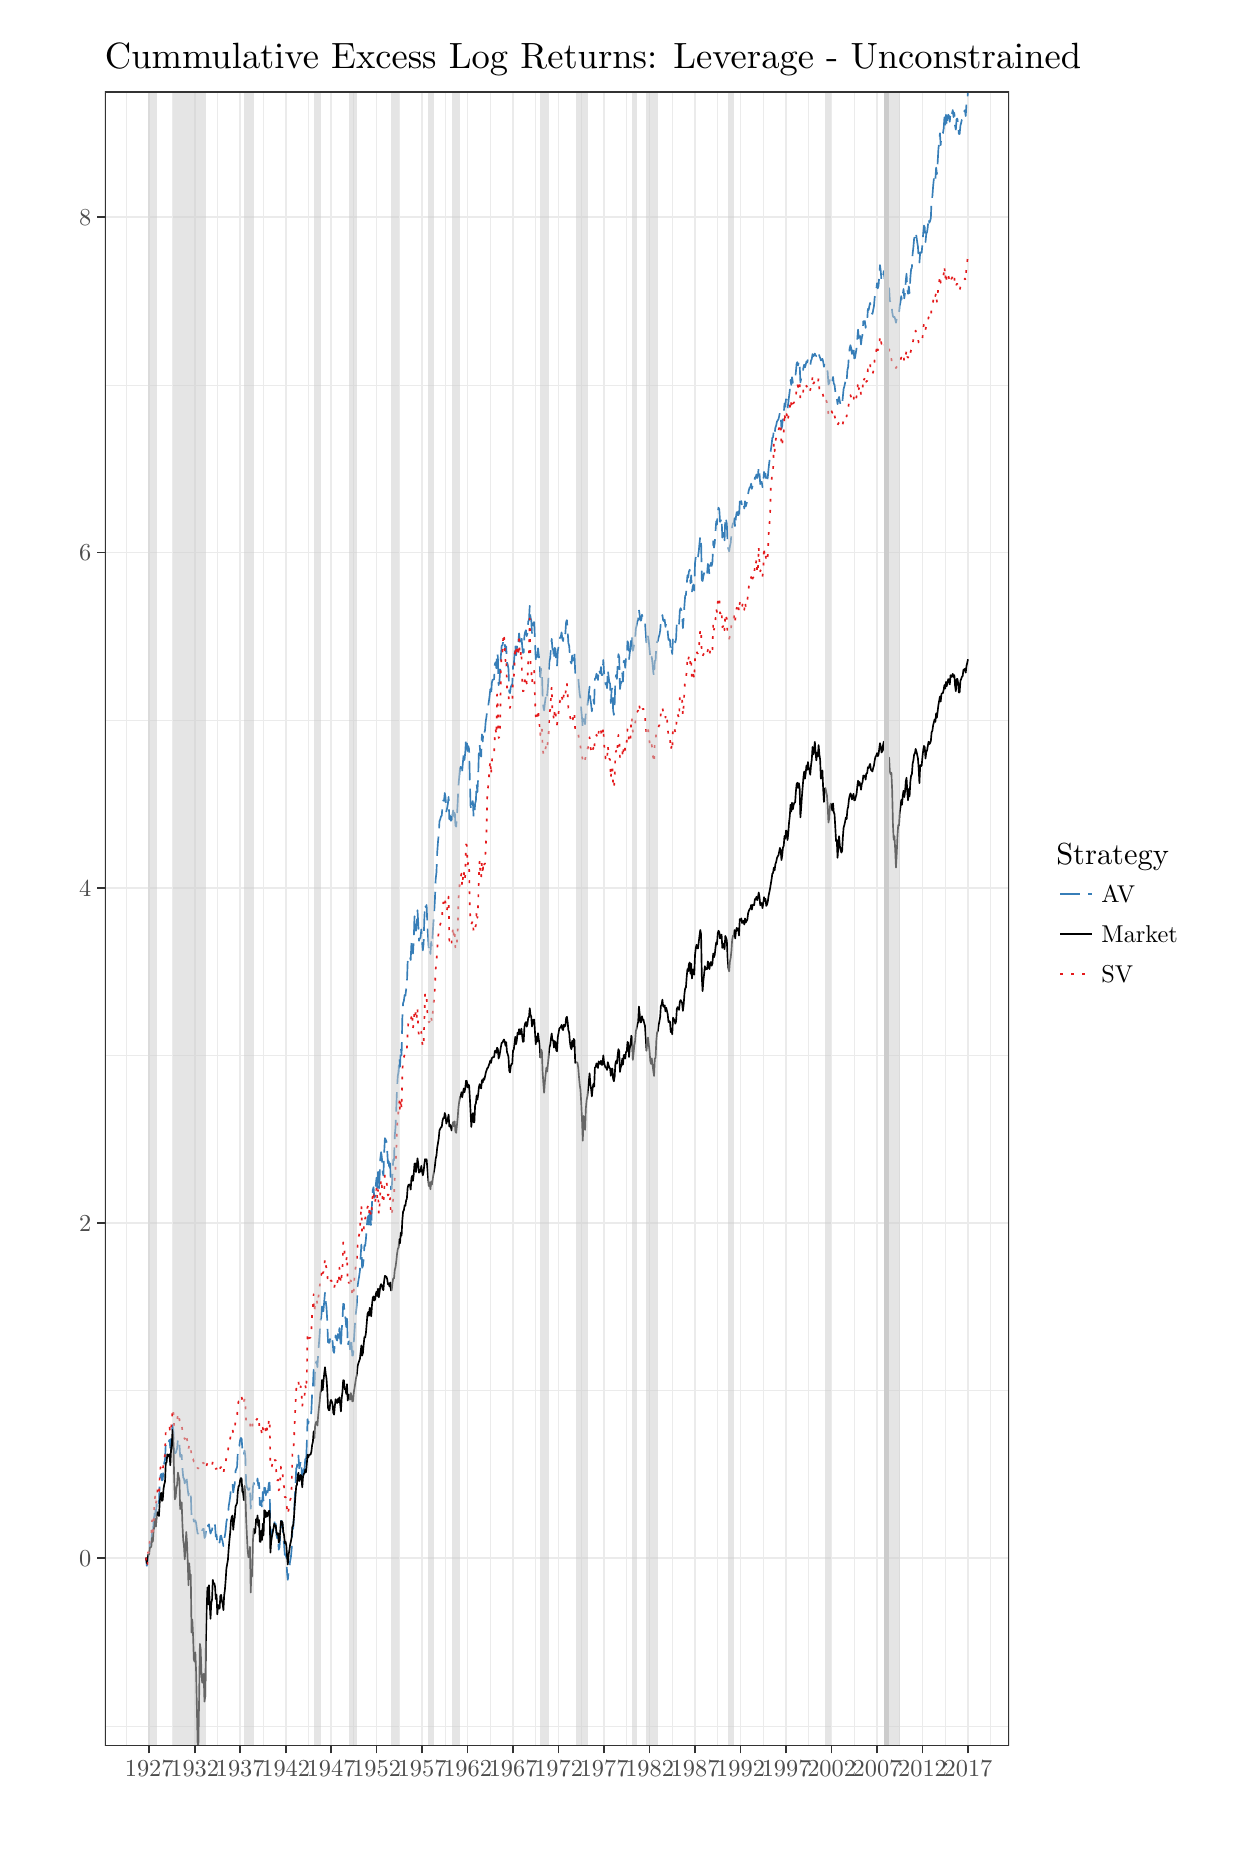
\begin{tikzpicture}[x=1pt,y=1pt]
\definecolor{fillColor}{RGB}{255,255,255}
\path[use as bounding box,fill=fillColor,fill opacity=0.00] (0,0) rectangle (426.79,650.43);
\begin{scope}
\path[clip] (  0.00,  0.00) rectangle (426.79,650.43);
\definecolor{drawColor}{RGB}{255,255,255}
\definecolor{fillColor}{RGB}{255,255,255}

\path[draw=drawColor,line width= 0.6pt,line join=round,line cap=round,fill=fillColor] (  0.00,  0.00) rectangle (426.79,650.43);
\end{scope}
\begin{scope}
\path[clip] ( 27.92, 29.59) rectangle (354.63,627.29);
\definecolor{fillColor}{RGB}{255,255,255}

\path[fill=fillColor] ( 27.92, 29.59) rectangle (354.63,627.29);
\definecolor{drawColor}{gray}{0.92}

\path[draw=drawColor,line width= 0.3pt,line join=round] ( 27.92, 36.76) --
	(354.63, 36.76);

\path[draw=drawColor,line width= 0.3pt,line join=round] ( 27.92,157.90) --
	(354.63,157.90);

\path[draw=drawColor,line width= 0.3pt,line join=round] ( 27.92,279.04) --
	(354.63,279.04);

\path[draw=drawColor,line width= 0.3pt,line join=round] ( 27.92,400.18) --
	(354.63,400.18);

\path[draw=drawColor,line width= 0.3pt,line join=round] ( 27.92,521.33) --
	(354.63,521.33);

\path[draw=drawColor,line width= 0.3pt,line join=round] ( 35.69, 29.59) --
	( 35.69,627.29);

\path[draw=drawColor,line width= 0.3pt,line join=round] ( 52.13, 29.59) --
	( 52.13,627.29);

\path[draw=drawColor,line width= 0.3pt,line join=round] ( 68.57, 29.59) --
	( 68.57,627.29);

\path[draw=drawColor,line width= 0.3pt,line join=round] ( 85.01, 29.59) --
	( 85.01,627.29);

\path[draw=drawColor,line width= 0.3pt,line join=round] (101.45, 29.59) --
	(101.45,627.29);

\path[draw=drawColor,line width= 0.3pt,line join=round] (117.88, 29.59) --
	(117.88,627.29);

\path[draw=drawColor,line width= 0.3pt,line join=round] (134.32, 29.59) --
	(134.32,627.29);

\path[draw=drawColor,line width= 0.3pt,line join=round] (150.77, 29.59) --
	(150.77,627.29);

\path[draw=drawColor,line width= 0.3pt,line join=round] (167.20, 29.59) --
	(167.20,627.29);

\path[draw=drawColor,line width= 0.3pt,line join=round] (183.64, 29.59) --
	(183.64,627.29);

\path[draw=drawColor,line width= 0.3pt,line join=round] (200.08, 29.59) --
	(200.08,627.29);

\path[draw=drawColor,line width= 0.3pt,line join=round] (216.52, 29.59) --
	(216.52,627.29);

\path[draw=drawColor,line width= 0.3pt,line join=round] (232.96, 29.59) --
	(232.96,627.29);

\path[draw=drawColor,line width= 0.3pt,line join=round] (249.39, 29.59) --
	(249.39,627.29);

\path[draw=drawColor,line width= 0.3pt,line join=round] (265.84, 29.59) --
	(265.84,627.29);

\path[draw=drawColor,line width= 0.3pt,line join=round] (282.28, 29.59) --
	(282.28,627.29);

\path[draw=drawColor,line width= 0.3pt,line join=round] (298.71, 29.59) --
	(298.71,627.29);

\path[draw=drawColor,line width= 0.3pt,line join=round] (315.15, 29.59) --
	(315.15,627.29);

\path[draw=drawColor,line width= 0.3pt,line join=round] (331.59, 29.59) --
	(331.59,627.29);

\path[draw=drawColor,line width= 0.3pt,line join=round] (348.03, 29.59) --
	(348.03,627.29);

\path[draw=drawColor,line width= 0.6pt,line join=round] ( 27.92, 97.33) --
	(354.63, 97.33);

\path[draw=drawColor,line width= 0.6pt,line join=round] ( 27.92,218.47) --
	(354.63,218.47);

\path[draw=drawColor,line width= 0.6pt,line join=round] ( 27.92,339.61) --
	(354.63,339.61);

\path[draw=drawColor,line width= 0.6pt,line join=round] ( 27.92,460.75) --
	(354.63,460.75);

\path[draw=drawColor,line width= 0.6pt,line join=round] ( 27.92,581.90) --
	(354.63,581.90);

\path[draw=drawColor,line width= 0.6pt,line join=round] ( 43.91, 29.59) --
	( 43.91,627.29);

\path[draw=drawColor,line width= 0.6pt,line join=round] ( 60.35, 29.59) --
	( 60.35,627.29);

\path[draw=drawColor,line width= 0.6pt,line join=round] ( 76.79, 29.59) --
	( 76.79,627.29);

\path[draw=drawColor,line width= 0.6pt,line join=round] ( 93.23, 29.59) --
	( 93.23,627.29);

\path[draw=drawColor,line width= 0.6pt,line join=round] (109.66, 29.59) --
	(109.66,627.29);

\path[draw=drawColor,line width= 0.6pt,line join=round] (126.10, 29.59) --
	(126.10,627.29);

\path[draw=drawColor,line width= 0.6pt,line join=round] (142.55, 29.59) --
	(142.55,627.29);

\path[draw=drawColor,line width= 0.6pt,line join=round] (158.98, 29.59) --
	(158.98,627.29);

\path[draw=drawColor,line width= 0.6pt,line join=round] (175.42, 29.59) --
	(175.42,627.29);

\path[draw=drawColor,line width= 0.6pt,line join=round] (191.86, 29.59) --
	(191.86,627.29);

\path[draw=drawColor,line width= 0.6pt,line join=round] (208.30, 29.59) --
	(208.30,627.29);

\path[draw=drawColor,line width= 0.6pt,line join=round] (224.74, 29.59) --
	(224.74,627.29);

\path[draw=drawColor,line width= 0.6pt,line join=round] (241.18, 29.59) --
	(241.18,627.29);

\path[draw=drawColor,line width= 0.6pt,line join=round] (257.61, 29.59) --
	(257.61,627.29);

\path[draw=drawColor,line width= 0.6pt,line join=round] (274.06, 29.59) --
	(274.06,627.29);

\path[draw=drawColor,line width= 0.6pt,line join=round] (290.50, 29.59) --
	(290.50,627.29);

\path[draw=drawColor,line width= 0.6pt,line join=round] (306.93, 29.59) --
	(306.93,627.29);

\path[draw=drawColor,line width= 0.6pt,line join=round] (323.37, 29.59) --
	(323.37,627.29);

\path[draw=drawColor,line width= 0.6pt,line join=round] (339.81, 29.59) --
	(339.81,627.29);
\definecolor{drawColor}{RGB}{55,126,184}

\path[draw=drawColor,line width= 0.6pt,dash pattern=on 7pt off 3pt ,line join=round] ( 42.78, 97.57) --
	( 43.05, 94.59) --
	( 43.32, 96.11) --
	( 43.60, 98.48) --
	( 43.87, 98.42) --
	( 44.15,102.56) --
	( 44.43,102.68) --
	( 44.68,103.01) --
	( 44.96,107.53) --
	( 45.23,105.48) --
	( 45.51,111.01) --
	( 45.78,112.72) --
	( 46.06,115.94) --
	( 46.34,112.64) --
	( 46.61,117.38) --
	( 46.89,119.07) --
	( 47.16,118.63) --
	( 47.44,117.17) --
	( 47.72,125.04) --
	( 47.98,127.09) --
	( 48.26,127.84) --
	( 48.53,125.49) --
	( 48.81,125.71) --
	( 49.08,130.18) --
	( 49.36,131.89) --
	( 49.63,132.87) --
	( 49.90,138.80) --
	( 50.18,138.86) --
	( 50.45,140.21) --
	( 50.73,140.17) --
	( 51.01,139.66) --
	( 51.26,140.11) --
	( 51.54,137.20) --
	( 51.81,140.50) --
	( 52.09,142.20) --
	( 52.36,145.46) --
	( 52.64,143.65) --
	( 52.92,135.79) --
	( 53.19,135.30) --
	( 53.47,135.37) --
	( 53.74,136.22) --
	( 54.02,137.15) --
	( 54.30,140.57) --
	( 54.55,139.60) --
	( 54.83,138.82) --
	( 55.10,134.01) --
	( 55.38,134.63) --
	( 55.65,134.66) --
	( 55.93,129.64) --
	( 56.21,126.55) --
	( 56.48,126.09) --
	( 56.75,124.42) --
	( 57.02,125.43) --
	( 57.30,127.39) --
	( 57.58,124.84) --
	( 57.83,122.24) --
	( 58.11,120.05) --
	( 58.38,121.80) --
	( 58.66,121.14) --
	( 58.93,121.20) --
	( 59.21,112.46) --
	( 59.49,113.21) --
	( 59.76,112.74) --
	( 60.04,110.65) --
	( 60.31,110.57) --
	( 60.59,111.03) --
	( 60.87,110.06) --
	( 61.13,108.12) --
	( 61.41,106.31) --
	( 61.68,106.27) --
	( 61.96,107.69) --
	( 62.23,108.33) --
	( 62.51,108.18) --
	( 62.79,107.75) --
	( 63.06,107.48) --
	( 63.33,107.90) --
	( 63.60,107.99) --
	( 63.88,104.68) --
	( 64.16,105.14) --
	( 64.41,107.10) --
	( 64.69,108.51) --
	( 64.96,109.81) --
	( 65.24,108.88) --
	( 65.51,109.62) --
	( 65.79,107.69) --
	( 66.07,106.31) --
	( 66.34,107.20) --
	( 66.62,107.51) --
	( 66.89,110.23) --
	( 67.17,109.67) --
	( 67.45,109.78) --
	( 67.70,109.21) --
	( 67.98,105.23) --
	( 68.25,105.85) --
	( 68.53,102.58) --
	( 68.80,103.64) --
	( 69.08,103.58) --
	( 69.36,102.99) --
	( 69.63,105.39) --
	( 69.91,105.53) --
	( 70.18,104.31) --
	( 70.45,103.38) --
	( 70.73,101.73) --
	( 70.99,104.25) --
	( 71.26,105.48) --
	( 71.53,107.40) --
	( 71.81,110.42) --
	( 72.08,111.76) --
	( 72.36,112.57) --
	( 72.64,116.13) --
	( 72.91,117.81) --
	( 73.19,119.69) --
	( 73.46,122.71) --
	( 73.74,123.84) --
	( 74.02,124.26) --
	( 74.28,121.15) --
	( 74.56,123.01) --
	( 74.83,124.20) --
	( 75.11,128.89) --
	( 75.38,129.60) --
	( 75.66,130.34) --
	( 75.94,135.88) --
	( 76.21,137.91) --
	( 76.49,138.02) --
	( 76.76,140.03) --
	( 77.03,140.82) --
	( 77.31,140.61) --
	( 77.57,136.91) --
	( 77.84,136.65) --
	( 78.11,134.52) --
	( 78.39,136.28) --
	( 78.66,134.14) --
	( 78.94,124.46) --
	( 79.22,122.97) --
	( 79.49,122.39) --
	( 79.77,121.99) --
	( 80.04,122.17) --
	( 80.32,123.46) --
	( 80.60,115.27) --
	( 80.85,117.89) --
	( 81.13,117.32) --
	( 81.40,123.09) --
	( 81.68,124.60) --
	( 81.95,123.82) --
	( 82.23,123.93) --
	( 82.51,125.04) --
	( 82.78,124.39) --
	( 83.06,126.19) --
	( 83.33,123.63) --
	( 83.61,124.64) --
	( 83.88,116.62) --
	( 84.14,116.56) --
	( 84.42,118.15) --
	( 84.69,115.21) --
	( 84.96,121.30) --
	( 85.23,117.87) --
	( 85.51,122.81) --
	( 85.79,122.77) --
	( 86.06,120.05) --
	( 86.34,122.78) --
	( 86.61,120.76) --
	( 86.89,122.07) --
	( 87.17,124.59) --
	( 87.43,124.67) --
	( 87.71,104.92) --
	( 87.98,105.70) --
	( 88.26,106.37) --
	( 88.53,108.11) --
	( 88.81,109.25) --
	( 89.09,110.76) --
	( 89.36,109.58) --
	( 89.64,109.81) --
	( 89.91,105.63) --
	( 90.19,104.55) --
	( 90.46,105.16) --
	( 90.72,100.45) --
	( 91.00,101.33) --
	( 91.27,105.55) --
	( 91.54,110.83) --
	( 91.81,110.74) --
	( 92.09,109.79) --
	( 92.37,104.39) --
	( 92.64,102.64) --
	( 92.92, 98.54) --
	( 93.19, 98.75) --
	( 93.47, 97.58) --
	( 93.75, 91.88) --
	( 94.00, 89.56) --
	( 94.28, 92.48) --
	( 94.55, 94.00) --
	( 94.83, 96.37) --
	( 95.10, 97.65) --
	( 95.38,100.53) --
	( 95.66,107.97) --
	( 95.93,108.03) --
	( 96.21,112.61) --
	( 96.48,118.20) --
	( 96.76,123.77) --
	( 97.04,129.75) --
	( 97.29,130.25) --
	( 97.57,133.30) --
	( 97.84,134.48) --
	( 98.12,129.84) --
	( 98.39,130.73) --
	( 98.67,132.62) --
	( 98.94,131.11) --
	( 99.21,123.76) --
	( 99.49,127.88) --
	( 99.76,129.41) --
	(100.04,129.81) --
	(100.32,133.25) --
	(100.58,131.24) --
	(100.86,138.64) --
	(101.13,147.61) --
	(101.41,145.99) --
	(101.68,147.59) --
	(101.96,147.61) --
	(102.24,147.81) --
	(102.51,150.51) --
	(102.79,156.99) --
	(103.06,159.09) --
	(103.34,165.49) --
	(103.62,159.65) --
	(103.87,166.12) --
	(104.15,168.05) --
	(104.42,168.51) --
	(104.70,166.39) --
	(104.97,171.39) --
	(105.25,174.86) --
	(105.52,178.58) --
	(105.79,183.33) --
	(106.07,184.23) --
	(106.34,188.31) --
	(106.62,184.86) --
	(106.90,187.16) --
	(107.15,190.08) --
	(107.43,193.28) --
	(107.70,190.19) --
	(107.98,187.99) --
	(108.25,183.18) --
	(108.53,175.45) --
	(108.81,175.22) --
	(109.08,175.23) --
	(109.36,177.37) --
	(109.63,177.87) --
	(109.91,177.14) --
	(110.19,175.61) --
	(110.44,172.26) --
	(110.72,171.58) --
	(110.99,174.77) --
	(111.27,177.89) --
	(111.54,176.57) --
	(111.82,176.02) --
	(112.10,178.39) --
	(112.37,176.42) --
	(112.64,180.53) --
	(112.91,177.20) --
	(113.19,173.28) --
	(113.47,180.09) --
	(113.73,182.71) --
	(114.01,189.29) --
	(114.28,189.20) --
	(114.56,184.24) --
	(114.83,184.44) --
	(115.11,180.93) --
	(115.39,185.49) --
	(115.66,174.19) --
	(115.94,175.54) --
	(116.21,175.79) --
	(116.49,172.81) --
	(116.77,176.93) --
	(117.02,174.92) --
	(117.30,170.54) --
	(117.57,170.71) --
	(117.85,175.52) --
	(118.12,179.91) --
	(118.40,183.75) --
	(118.68,186.70) --
	(118.95,189.08) --
	(119.22,195.60) --
	(119.49,197.58) --
	(119.77,199.17) --
	(120.05,201.19) --
	(120.30,206.06) --
	(120.58,210.72) --
	(120.85,202.30) --
	(121.13,202.91) --
	(121.40,205.39) --
	(121.68,210.49) --
	(121.96,210.24) --
	(122.23,212.75) --
	(122.51,216.63) --
	(122.78,220.04) --
	(123.06,221.07) --
	(123.34,217.88) --
	(123.59,222.92) --
	(123.87,219.84) --
	(124.14,217.00) --
	(124.42,225.56) --
	(124.69,230.37) --
	(124.97,231.42) --
	(125.25,227.63) --
	(125.52,228.04) --
	(125.80,232.17) --
	(126.07,234.87) --
	(126.34,231.14) --
	(126.62,236.99) --
	(126.88,230.34) --
	(127.16,234.87) --
	(127.43,241.73) --
	(127.71,244.09) --
	(127.98,242.33) --
	(128.26,236.97) --
	(128.54,235.65) --
	(128.81,243.70) --
	(129.09,249.14) --
	(129.36,248.63) --
	(129.64,247.91) --
	(129.92,244.64) --
	(130.17,240.13) --
	(130.45,240.79) --
	(130.72,237.07) --
	(131.00,240.06) --
	(131.27,230.63) --
	(131.55,230.93) --
	(131.83,236.52) --
	(132.10,241.35) --
	(132.38,241.22) --
	(132.65,250.14) --
	(132.92,253.11) --
	(133.20,260.16) --
	(133.46,266.95) --
	(133.73,271.47) --
	(134.00,273.25) --
	(134.28,278.19) --
	(134.55,274.98) --
	(134.83,281.84) --
	(135.11,279.14) --
	(135.38,292.53) --
	(135.66,298.02) --
	(135.93,298.70) --
	(136.21,300.85) --
	(136.49,300.62) --
	(136.74,302.79) --
	(137.02,304.34) --
	(137.29,312.48) --
	(137.57,314.90) --
	(137.84,315.16) --
	(138.12,314.77) --
	(138.40,313.53) --
	(138.67,319.56) --
	(138.95,320.89) --
	(139.22,315.85) --
	(139.50,320.50) --
	(139.77,329.18) --
	(140.04,329.55) --
	(140.31,324.06) --
	(140.58,327.12) --
	(140.86,331.48) --
	(141.13,326.87) --
	(141.41,320.47) --
	(141.69,321.31) --
	(141.96,321.60) --
	(142.24,324.58) --
	(142.51,320.04) --
	(142.79,317.02) --
	(143.07,319.59) --
	(143.32,328.23) --
	(143.60,333.57) --
	(143.87,332.57) --
	(144.15,333.40) --
	(144.42,326.50) --
	(144.70,321.40) --
	(144.98,316.82) --
	(145.25,317.70) --
	(145.53,315.71) --
	(145.80,320.10) --
	(146.08,318.35) --
	(146.35,322.86) --
	(146.61,327.40) --
	(146.89,330.65) --
	(147.16,335.49) --
	(147.43,342.79) --
	(147.71,345.17) --
	(147.98,352.27) --
	(148.26,356.13) --
	(148.53,359.01) --
	(148.81,363.71) --
	(149.08,364.39) --
	(149.36,365.41) --
	(149.64,365.72) --
	(149.89,369.43) --
	(150.17,371.21) --
	(150.44,371.06) --
	(150.72,373.85) --
	(150.99,372.36) --
	(151.27,367.19) --
	(151.55,368.31) --
	(151.82,369.85) --
	(152.10,372.47) --
	(152.37,364.32) --
	(152.65,365.64) --
	(152.93,364.08) --
	(153.19,362.35) --
	(153.47,365.75) --
	(153.74,367.59) --
	(154.02,365.59) --
	(154.29,368.34) --
	(154.56,362.22) --
	(154.84,361.72) --
	(155.11,365.60) --
	(155.39,370.60) --
	(155.66,376.49) --
	(155.94,379.69) --
	(156.22,382.82) --
	(156.47,383.22) --
	(156.75,384.98) --
	(157.02,381.95) --
	(157.30,385.26) --
	(157.57,388.27) --
	(157.85,385.80) --
	(158.13,388.68) --
	(158.40,393.61) --
	(158.68,393.48) --
	(158.95,389.06) --
	(159.23,390.79) --
	(159.51,389.69) --
	(159.76,378.99) --
	(160.04,369.26) --
	(160.31,367.54) --
	(160.59,369.47) --
	(160.86,370.97) --
	(161.14,365.20) --
	(161.41,365.18) --
	(161.68,370.12) --
	(161.96,371.02) --
	(162.23,377.27) --
	(162.51,374.18) --
	(162.79,379.93) --
	(163.04,388.61) --
	(163.32,391.29) --
	(163.59,387.81) --
	(163.87,387.01) --
	(164.14,395.06) --
	(164.42,392.49) --
	(164.70,396.47) --
	(164.97,395.54) --
	(165.25,396.47) --
	(165.52,399.80) --
	(165.80,401.55) --
	(166.08,404.44) --
	(166.34,404.79) --
	(166.62,406.77) --
	(166.89,408.74) --
	(167.17,411.40) --
	(167.44,408.83) --
	(167.72,413.67) --
	(167.99,414.79) --
	(168.26,414.84) --
	(168.54,414.98) --
	(168.81,420.39) --
	(169.09,421.14) --
	(169.37,418.93) --
	(169.62,424.65) --
	(169.90,423.09) --
	(170.17,412.84) --
	(170.45,414.01) --
	(170.72,418.15) --
	(171.00,423.53) --
	(171.28,427.19) --
	(171.55,427.18) --
	(171.83,428.60) --
	(172.10,429.48) --
	(172.38,428.04) --
	(172.66,425.07) --
	(172.91,426.80) --
	(173.19,421.07) --
	(173.46,420.27) --
	(173.74,418.68) --
	(174.01,410.46) --
	(174.29,409.97) --
	(174.57,412.22) --
	(174.84,412.81) --
	(175.11,412.96) --
	(175.38,419.65) --
	(175.66,420.19) --
	(175.94,424.43) --
	(176.19,427.71) --
	(176.47,423.59) --
	(176.74,425.66) --
	(177.02,429.13) --
	(177.29,428.34) --
	(177.57,431.56) --
	(177.85,428.48) --
	(178.12,428.90) --
	(178.40,430.99) --
	(178.67,427.24) --
	(178.95,424.55) --
	(179.23,424.64) --
	(179.49,430.70) --
	(179.77,432.08) --
	(180.04,432.69) --
	(180.32,430.58) --
	(180.59,431.64) --
	(180.87,435.84) --
	(181.15,436.33) --
	(181.42,441.50) --
	(181.69,437.32) --
	(181.96,436.30) --
	(182.24,431.31) --
	(182.52,433.99) --
	(182.77,435.53) --
	(183.05,435.57) --
	(183.32,428.31) --
	(183.60,422.15) --
	(183.87,424.56) --
	(184.15,422.45) --
	(184.43,426.17) --
	(184.70,423.61) --
	(184.98,421.05) --
	(185.25,415.75) --
	(185.53,418.79) --
	(185.81,418.17) --
	(186.06,409.41) --
	(186.34,404.98) --
	(186.61,403.72) --
	(186.89,406.38) --
	(187.16,408.36) --
	(187.44,410.57) --
	(187.72,409.05) --
	(187.99,412.27) --
	(188.27,417.11) --
	(188.54,421.47) --
	(188.81,422.58) --
	(189.09,426.65) --
	(189.35,429.57) --
	(189.62,425.86) --
	(189.89,425.90) --
	(190.17,422.09) --
	(190.44,426.34) --
	(190.72,425.87) --
	(191.00,420.19) --
	(191.27,419.70) --
	(191.55,424.99) --
	(191.82,426.76) --
	(192.10,429.42) --
	(192.38,430.04) --
	(192.64,430.33) --
	(192.92,431.91) --
	(193.19,429.59) --
	(193.47,428.76) --
	(193.74,431.81) --
	(194.02,430.96) --
	(194.30,431.65) --
	(194.57,435.68) --
	(194.85,436.35) --
	(195.12,432.34) --
	(195.39,427.98) --
	(195.67,427.09) --
	(195.93,423.23) --
	(196.20,421.30) --
	(196.47,420.67) --
	(196.75,423.57) --
	(197.02,421.68) --
	(197.30,424.97) --
	(197.58,424.50) --
	(197.85,417.24) --
	(198.13,417.41) --
	(198.40,417.38) --
	(198.68,417.25) --
	(198.96,415.54) --
	(199.21,412.37) --
	(199.49,409.47) --
	(199.76,408.09) --
	(200.04,403.88) --
	(200.31,400.98) --
	(200.59,397.31) --
	(200.87,400.63) --
	(201.14,399.81) --
	(201.42,398.72) --
	(201.69,403.07) --
	(201.97,404.51) --
	(202.24,405.56) --
	(202.50,407.52) --
	(202.78,409.84) --
	(203.05,412.30) --
	(203.32,407.90) --
	(203.60,405.86) --
	(203.87,403.39) --
	(204.15,406.13) --
	(204.42,407.57) --
	(204.70,406.04) --
	(204.97,415.20) --
	(205.25,415.36) --
	(205.53,416.98) --
	(205.79,415.98) --
	(206.07,414.72) --
	(206.34,418.81) --
	(206.62,417.84) --
	(206.89,417.12) --
	(207.17,419.43) --
	(207.45,416.46) --
	(207.72,416.56) --
	(208.00,421.94) --
	(208.27,417.35) --
	(208.55,415.05) --
	(208.82,413.17) --
	(209.08,413.35) --
	(209.36,411.75) --
	(209.63,418.40) --
	(209.91,416.06) --
	(210.18,413.79) --
	(210.45,413.45) --
	(210.73,406.34) --
	(211.00,411.28) --
	(211.28,411.60) --
	(211.55,403.77) --
	(211.83,402.08) --
	(212.11,406.28) --
	(212.36,414.98) --
	(212.64,416.53) --
	(212.91,415.09) --
	(213.19,420.12) --
	(213.46,424.03) --
	(213.74,423.06) --
	(214.02,411.44) --
	(214.29,413.32) --
	(214.57,413.91) --
	(214.84,417.39) --
	(215.12,414.14) --
	(215.40,421.57) --
	(215.65,421.70) --
	(215.93,419.09) --
	(216.20,422.62) --
	(216.48,423.28) --
	(216.75,428.69) --
	(217.03,428.04) --
	(217.30,422.04) --
	(217.57,424.69) --
	(217.85,426.01) --
	(218.12,430.99) --
	(218.40,430.67) --
	(218.68,425.28) --
	(218.94,426.38) --
	(219.22,428.22) --
	(219.49,429.61) --
	(219.77,433.34) --
	(220.04,434.39) --
	(220.32,435.88) --
	(220.60,436.43) --
	(220.87,440.13) --
	(221.15,438.02) --
	(221.42,436.14) --
	(221.70,436.27) --
	(221.98,438.31) --
	(222.23,437.40) --
	(222.51,437.47) --
	(222.78,436.28) --
	(223.06,435.68) --
	(223.33,431.79) --
	(223.61,427.74) --
	(223.88,429.39) --
	(224.15,430.52) --
	(224.43,428.74) --
	(224.70,425.87) --
	(224.98,422.83) --
	(225.26,421.70) --
	(225.51,423.07) --
	(225.79,420.64) --
	(226.06,417.63) --
	(226.34,415.96) --
	(226.61,421.66) --
	(226.89,421.83) --
	(227.17,427.32) --
	(227.44,428.48) --
	(227.72,428.76) --
	(227.99,430.13) --
	(228.27,430.96) --
	(228.55,432.49) --
	(228.80,435.84) --
	(229.08,436.28) --
	(229.35,438.19) --
	(229.63,436.21) --
	(229.90,436.02) --
	(230.18,436.52) --
	(230.46,433.90) --
	(230.73,435.22) --
	(231.00,433.89) --
	(231.27,432.28) --
	(231.55,429.17) --
	(231.83,429.46) --
	(232.09,429.19) --
	(232.37,424.76) --
	(232.64,425.84) --
	(232.92,424.10) --
	(233.19,430.63) --
	(233.47,430.28) --
	(233.75,429.58) --
	(234.02,428.27) --
	(234.30,429.59) --
	(234.57,435.69) --
	(234.85,436.40) --
	(235.13,435.66) --
	(235.38,435.00) --
	(235.66,439.84) --
	(235.93,440.66) --
	(236.21,439.98) --
	(236.48,439.13) --
	(236.76,433.42) --
	(237.04,437.19) --
	(237.31,441.50) --
	(237.58,445.12) --
	(237.85,445.38) --
	(238.13,449.15) --
	(238.41,452.50) --
	(238.66,451.68) --
	(238.94,453.89) --
	(239.21,454.55) --
	(239.49,449.65) --
	(239.76,452.53) --
	(240.04,446.67) --
	(240.32,448.49) --
	(240.59,449.22) --
	(240.87,447.03) --
	(241.14,456.91) --
	(241.42,459.26) --
	(241.70,460.56) --
	(241.95,459.28) --
	(242.23,459.29) --
	(242.50,461.21) --
	(242.78,464.28) --
	(243.05,466.72) --
	(243.33,465.06) --
	(243.61,450.82) --
	(243.88,450.48) --
	(244.16,452.21) --
	(244.43,453.33) --
	(244.70,454.49) --
	(244.98,453.25) --
	(245.24,453.62) --
	(245.52,453.39) --
	(245.79,456.64) --
	(246.07,455.78) --
	(246.34,452.87) --
	(246.62,455.91) --
	(246.90,457.07) --
	(247.17,455.92) --
	(247.45,457.40) --
	(247.72,464.89) --
	(248.00,462.54) --
	(248.28,464.27) --
	(248.53,468.17) --
	(248.81,472.07) --
	(249.08,470.86) --
	(249.36,475.56) --
	(249.63,476.99) --
	(249.91,476.31) --
	(250.19,471.86) --
	(250.46,472.26) --
	(250.74,473.36) --
	(251.01,466.14) --
	(251.28,466.65) --
	(251.56,468.34) --
	(251.82,465.15) --
	(252.09,473.63) --
	(252.36,472.59) --
	(252.64,471.18) --
	(252.91,464.09) --
	(253.19,462.23) --
	(253.47,461.18) --
	(253.74,463.00) --
	(254.02,464.19) --
	(254.29,467.28) --
	(254.57,470.17) --
	(254.85,471.30) --
	(255.10,471.21) --
	(255.38,473.17) --
	(255.65,469.77) --
	(255.93,473.58) --
	(256.20,475.34) --
	(256.48,474.30) --
	(256.76,475.62) --
	(257.03,472.82) --
	(257.31,479.21) --
	(257.58,478.92) --
	(257.86,479.38) --
	(258.13,477.47) --
	(258.40,478.51) --
	(258.67,478.67) --
	(258.94,476.68) --
	(259.22,479.30) --
	(259.49,477.44) --
	(259.77,478.50) --
	(260.05,479.23) --
	(260.32,481.93) --
	(260.60,483.33) --
	(260.87,484.23) --
	(261.15,484.43) --
	(261.43,485.68) --
	(261.68,483.75) --
	(261.96,484.98) --
	(262.23,485.22) --
	(262.51,485.00) --
	(262.78,487.89) --
	(263.06,487.75) --
	(263.34,488.98) --
	(263.61,487.66) --
	(263.89,488.82) --
	(264.16,491.61) --
	(264.44,489.51) --
	(264.71,485.48) --
	(264.97,485.97) --
	(265.25,486.32) --
	(265.52,484.38) --
	(265.80,486.45) --
	(266.07,489.91) --
	(266.34,488.25) --
	(266.62,489.31) --
	(266.89,485.93) --
	(267.17,486.65) --
	(267.44,488.04) --
	(267.72,491.09) --
	(268.00,493.48) --
	(268.25,495.26) --
	(268.53,497.73) --
	(268.80,499.63) --
	(269.08,502.17) --
	(269.35,502.46) --
	(269.63,505.13) --
	(269.91,503.83) --
	(270.18,505.93) --
	(270.46,506.59) --
	(270.73,508.03) --
	(271.01,508.52) --
	(271.29,508.95) --
	(271.55,510.02) --
	(271.83,511.38) --
	(272.10,510.46) --
	(272.38,505.42) --
	(272.65,506.59) --
	(272.92,509.96) --
	(273.20,510.73) --
	(273.47,514.64) --
	(273.75,513.46) --
	(274.02,516.16) --
	(274.30,515.86) --
	(274.58,512.87) --
	(274.83,514.69) --
	(275.11,517.10) --
	(275.38,519.27) --
	(275.66,523.16) --
	(275.93,521.34) --
	(276.21,524.10) --
	(276.49,522.10) --
	(276.76,522.69) --
	(277.04,523.34) --
	(277.31,523.37) --
	(277.59,526.05) --
	(277.87,529.16) --
	(278.12,529.55) --
	(278.40,528.38) --
	(278.67,530.09) --
	(278.95,528.86) --
	(279.22,522.27) --
	(279.50,523.53) --
	(279.77,524.64) --
	(280.04,525.49) --
	(280.32,527.67) --
	(280.59,528.64) --
	(280.87,527.67) --
	(281.15,528.62) --
	(281.40,529.84) --
	(281.68,529.42) --
	(281.95,530.66) --
	(282.23,529.71) --
	(282.50,529.16) --
	(282.78,528.34) --
	(283.06,530.07) --
	(283.33,530.72) --
	(283.61,532.47) --
	(283.88,531.67) --
	(284.16,531.97) --
	(284.44,532.66) --
	(284.70,532.05) --
	(284.98,531.71) --
	(285.25,532.32) --
	(285.53,531.98) --
	(285.80,533.10) --
	(286.08,531.75) --
	(286.35,531.16) --
	(286.62,530.17) --
	(286.90,530.38) --
	(287.17,530.76) --
	(287.45,529.74) --
	(287.73,527.89) --
	(287.98,528.96) --
	(288.26,529.04) --
	(288.53,528.36) --
	(288.81,527.57) --
	(289.08,525.77) --
	(289.36,521.50) --
	(289.64,521.98) --
	(289.91,523.63) --
	(290.19,524.25) --
	(290.46,523.45) --
	(290.74,522.54) --
	(291.02,524.22) --
	(291.27,521.85) --
	(291.55,521.39) --
	(291.82,519.11) --
	(292.10,516.52) --
	(292.37,516.59) --
	(292.65,514.39) --
	(292.93,516.20) --
	(293.20,516.98) --
	(293.47,515.42) --
	(293.74,514.16) --
	(294.02,513.60) --
	(294.30,514.15) --
	(294.55,516.89) --
	(294.83,519.90) --
	(295.10,520.75) --
	(295.38,522.12) --
	(295.65,523.49) --
	(295.93,522.56) --
	(296.21,526.74) --
	(296.48,527.84) --
	(296.76,532.28) --
	(297.03,534.64) --
	(297.31,535.68) --
	(297.59,534.48) --
	(297.85,532.53) --
	(298.13,533.48) --
	(298.40,535.45) --
	(298.68,530.91) --
	(298.95,531.07) --
	(299.23,532.82) --
	(299.51,534.51) --
	(299.78,537.92) --
	(300.05,541.30) --
	(300.32,538.26) --
	(300.60,540.40) --
	(300.88,538.45) --
	(301.13,535.96) --
	(301.41,538.42) --
	(301.68,539.50) --
	(301.96,544.39) --
	(302.23,543.52) --
	(302.51,544.44) --
	(302.79,541.95) --
	(303.06,544.08) --
	(303.34,544.15) --
	(303.61,548.78) --
	(303.89,548.41) --
	(304.17,549.98) --
	(304.42,550.98) --
	(304.70,547.65) --
	(304.97,547.37) --
	(305.25,546.99) --
	(305.52,548.37) --
	(305.80,549.85) --
	(306.08,553.10) --
	(306.35,554.88) --
	(306.63,555.59) --
	(306.90,558.05) --
	(307.17,556.22) --
	(307.45,557.08) --
	(307.71,560.55) --
	(307.98,564.62) --
	(308.25,562.54) --
	(308.53,558.90) --
	(308.80,559.38) --
	(309.08,560.65) --
	(309.36,562.47) --
	(309.63,559.65) --
	(309.91,559.44) --
	(310.18,555.46) --
	(310.46,554.81) --
	(310.74,554.33) --
	(311.00,555.51) --
	(311.28,556.31) --
	(311.55,551.76) --
	(311.83,551.12) --
	(312.10,551.26) --
	(312.38,547.78) --
	(312.66,546.13) --
	(312.93,545.79) --
	(313.21,545.92) --
	(313.48,545.09) --
	(313.75,543.80) --
	(314.03,545.22) --
	(314.29,546.16) --
	(314.56,547.19) --
	(314.84,547.13) --
	(315.11,550.02) --
	(315.38,551.15) --
	(315.66,553.42) --
	(315.94,551.80) --
	(316.21,554.01) --
	(316.49,556.00) --
	(316.76,552.59) --
	(317.04,554.84) --
	(317.32,559.15) --
	(317.57,561.51) --
	(317.85,555.87) --
	(318.12,554.25) --
	(318.40,556.95) --
	(318.67,554.47) --
	(318.95,560.05) --
	(319.23,563.20) --
	(319.50,563.63) --
	(319.78,568.70) --
	(320.05,571.11) --
	(320.33,574.37) --
	(320.60,574.66) --
	(320.86,576.62) --
	(321.14,574.97) --
	(321.41,573.08) --
	(321.69,571.37) --
	(321.96,566.86) --
	(322.23,565.55) --
	(322.51,569.22) --
	(322.78,569.05) --
	(323.06,569.16) --
	(323.33,572.65) --
	(323.61,576.24) --
	(323.89,578.91) --
	(324.15,578.22) --
	(324.43,572.93) --
	(324.70,575.92) --
	(324.98,576.52) --
	(325.25,578.39) --
	(325.53,581.70) --
	(325.81,579.95) --
	(326.08,580.57) --
	(326.36,581.62) --
	(326.63,588.60) --
	(326.91,589.41) --
	(327.19,593.24) --
	(327.44,595.68) --
	(327.72,596.99) --
	(327.99,595.50) --
	(328.27,599.88) --
	(328.54,597.48) --
	(328.81,601.54) --
	(329.09,606.64) --
	(329.36,608.81) --
	(329.64,612.27) --
	(329.91,607.97) --
	(330.19,611.63) --
	(330.47,612.10) --
	(330.72,612.30) --
	(331.00,613.96) --
	(331.27,618.04) --
	(331.55,614.52) --
	(331.82,618.93) --
	(332.10,614.77) --
	(332.38,617.81) --
	(332.65,618.97) --
	(332.93,618.49) --
	(333.20,616.43) --
	(333.48,619.92) --
	(333.76,618.82) --
	(334.01,619.55) --
	(334.29,620.66) --
	(334.56,618.10) --
	(334.84,619.69) --
	(335.11,615.00) --
	(335.39,613.59) --
	(335.66,617.39) --
	(335.93,617.54) --
	(336.21,615.60) --
	(336.48,611.99) --
	(336.76,612.01) --
	(337.04,615.01) --
	(337.30,616.04) --
	(337.58,617.19) --
	(337.85,617.50) --
	(338.13,619.82) --
	(338.40,620.16) --
	(338.68,620.59) --
	(338.96,618.46) --
	(339.23,623.12) --
	(339.51,624.25) --
	(339.78,627.29);
\definecolor{drawColor}{RGB}{0,0,0}

\path[draw=drawColor,line width= 0.6pt,line join=round] ( 42.78, 97.55) --
	( 43.05, 95.61) --
	( 43.32, 97.18) --
	( 43.60, 98.73) --
	( 43.87, 98.69) --
	( 44.15,101.21) --
	( 44.43,101.28) --
	( 44.68,101.56) --
	( 44.96,104.78) --
	( 45.23,103.34) --
	( 45.51,107.55) --
	( 45.78,108.74) --
	( 46.06,111.51) --
	( 46.34,108.82) --
	( 46.61,112.71) --
	( 46.89,113.98) --
	( 47.16,113.65) --
	( 47.44,112.63) --
	( 47.72,117.73) --
	( 47.98,120.13) --
	( 48.26,121.01) --
	( 48.53,118.08) --
	( 48.81,118.45) --
	( 49.08,122.37) --
	( 49.36,124.06) --
	( 49.63,125.02) --
	( 49.90,131.80) --
	( 50.18,131.89) --
	( 50.45,134.84) --
	( 50.73,134.78) --
	( 51.01,134.10) --
	( 51.26,134.91) --
	( 51.54,130.96) --
	( 51.81,136.60) --
	( 52.09,139.06) --
	( 52.36,143.71) --
	( 52.64,140.37) --
	( 52.92,126.86) --
	( 53.19,118.65) --
	( 53.47,119.35) --
	( 53.74,122.57) --
	( 54.02,124.03) --
	( 54.30,128.30) --
	( 54.55,126.87) --
	( 54.83,125.80) --
	( 55.10,115.11) --
	( 55.38,117.45) --
	( 55.65,117.50) --
	( 55.93,109.31) --
	( 56.21,103.77) --
	( 56.48,101.91) --
	( 56.75, 96.96) --
	( 57.02,100.62) --
	( 57.30,106.84) --
	( 57.58,102.82) --
	( 57.83, 96.40) --
	( 58.11, 87.62) --
	( 58.38, 95.52) --
	( 58.66, 91.30) --
	( 58.93, 91.44) --
	( 59.21, 70.51) --
	( 59.49, 75.24) --
	( 59.76, 69.62) --
	( 60.04, 60.77) --
	( 60.31, 60.03) --
	( 60.59, 63.35) --
	( 60.87, 56.11) --
	( 61.13, 44.00) --
	( 61.41, 29.91) --
	( 61.68, 29.59) --
	( 61.96, 47.31) --
	( 62.23, 66.42) --
	( 62.51, 64.65) --
	( 62.79, 56.01) --
	( 63.06, 52.36) --
	( 63.33, 55.03) --
	( 63.60, 55.61) --
	( 63.88, 45.53) --
	( 64.16, 47.49) --
	( 64.41, 67.64) --
	( 64.69, 79.32) --
	( 64.96, 86.85) --
	( 65.24, 80.69) --
	( 65.51, 87.61) --
	( 65.79, 80.82) --
	( 66.07, 75.51) --
	( 66.34, 81.27) --
	( 66.62, 82.33) --
	( 66.89, 89.55) --
	( 67.17, 88.05) --
	( 67.45, 88.29) --
	( 67.70, 87.15) --
	( 67.98, 82.60) --
	( 68.25, 84.11) --
	( 68.53, 77.09) --
	( 68.80, 80.44) --
	( 69.08, 80.29) --
	( 69.36, 79.13) --
	( 69.63, 83.90) --
	( 69.91, 84.11) --
	( 70.18, 82.05) --
	( 70.45, 80.85) --
	( 70.73, 78.62) --
	( 70.99, 83.85) --
	( 71.26, 85.91) --
	( 71.53, 89.30) --
	( 71.81, 93.63) --
	( 72.08, 95.22) --
	( 72.36, 96.78) --
	( 72.64,100.84) --
	( 72.91,103.95) --
	( 73.19,106.72) --
	( 73.46,110.79) --
	( 73.74,112.30) --
	( 74.02,112.79) --
	( 74.28,107.64) --
	( 74.56,110.70) --
	( 74.83,112.16) --
	( 75.11,116.02) --
	( 75.38,116.66) --
	( 75.66,117.37) --
	( 75.94,121.46) --
	( 76.21,123.41) --
	( 76.49,123.56) --
	( 76.76,125.54) --
	( 77.03,126.33) --
	( 77.31,126.16) --
	( 77.57,121.40) --
	( 77.84,120.96) --
	( 78.11,118.36) --
	( 78.39,123.53) --
	( 78.66,120.51) --
	( 78.94,111.59) --
	( 79.22,105.48) --
	( 79.49,100.20) --
	( 79.77, 97.67) --
	( 80.04, 98.07) --
	( 80.32,101.48) --
	( 80.60, 84.99) --
	( 80.85, 93.24) --
	( 81.13, 90.83) --
	( 81.40,103.75) --
	( 81.68,107.97) --
	( 81.95,106.30) --
	( 82.23,106.85) --
	( 82.51,111.45) --
	( 82.78,110.32) --
	( 83.06,112.80) --
	( 83.33,109.07) --
	( 83.61,111.17) --
	( 83.88,103.38) --
	( 84.14,103.26) --
	( 84.42,107.30) --
	( 84.69,103.96) --
	( 84.96,109.85) --
	( 85.23,105.63) --
	( 85.51,114.71) --
	( 85.79,114.47) --
	( 86.06,112.17) --
	( 86.34,113.94) --
	( 86.61,112.46) --
	( 86.89,113.34) --
	( 87.17,114.46) --
	( 87.43,114.51) --
	( 87.71, 99.38) --
	( 87.98,103.30) --
	( 88.26,105.21) --
	( 88.53,106.67) --
	( 88.81,108.04) --
	( 89.09,109.85) --
	( 89.36,108.83) --
	( 89.64,109.22) --
	( 89.91,106.67) --
	( 90.19,105.83) --
	( 90.46,106.41) --
	( 90.72,103.05) --
	( 91.00,103.84) --
	( 91.27,107.29) --
	( 91.54,110.79) --
	( 91.81,110.72) --
	( 92.09,110.24) --
	( 92.37,106.94) --
	( 92.64,105.69) --
	( 92.92,102.80) --
	( 93.19,103.34) --
	( 93.47,101.88) --
	( 93.75, 97.79) --
	( 94.00, 95.09) --
	( 94.28, 98.62) --
	( 94.55,100.15) --
	( 94.83,102.24) --
	( 95.10,103.33) --
	( 95.38,104.93) --
	( 95.66,108.96) --
	( 95.93,109.01) --
	( 96.21,112.02) --
	( 96.48,116.29) --
	( 96.76,119.83) --
	( 97.04,123.45) --
	( 97.29,123.87) --
	( 97.57,127.22) --
	( 97.84,128.24) --
	( 98.12,125.26) --
	( 98.39,126.05) --
	( 98.67,127.47) --
	( 98.94,126.75) --
	( 99.21,122.99) --
	( 99.49,126.74) --
	( 99.76,127.81) --
	(100.04,128.00) --
	(100.32,129.46) --
	(100.58,128.44) --
	(100.86,131.43) --
	(101.13,134.76) --
	(101.41,133.82) --
	(101.68,134.74) --
	(101.96,134.75) --
	(102.24,134.86) --
	(102.51,135.85) --
	(102.79,138.27) --
	(103.06,139.46) --
	(103.34,143.23) --
	(103.62,140.79) --
	(103.87,145.34) --
	(104.15,146.42) --
	(104.42,146.69) --
	(104.70,145.32) --
	(104.97,148.94) --
	(105.25,151.78) --
	(105.52,154.06) --
	(105.79,157.28) --
	(106.07,158.04) --
	(106.34,161.75) --
	(106.62,158.10) --
	(106.90,161.49) --
	(107.15,163.99) --
	(107.43,166.35) --
	(107.70,163.95) --
	(107.98,162.31) --
	(108.25,158.26) --
	(108.53,151.72) --
	(108.81,150.84) --
	(109.08,150.87) --
	(109.36,153.81) --
	(109.63,154.58) --
	(109.91,153.89) --
	(110.19,152.84) --
	(110.44,149.86) --
	(110.72,149.26) --
	(110.99,152.38) --
	(111.27,154.82) --
	(111.54,153.74) --
	(111.82,153.44) --
	(112.10,154.91) --
	(112.37,153.72) --
	(112.64,155.52) --
	(112.91,153.14) --
	(113.19,150.41) --
	(113.47,155.17) --
	(113.73,157.40) --
	(114.01,161.68) --
	(114.28,161.62) --
	(114.56,158.44) --
	(114.83,158.62) --
	(115.11,156.74) --
	(115.39,160.23) --
	(115.66,154.35) --
	(115.94,156.27) --
	(116.21,156.43) --
	(116.49,154.63) --
	(116.77,157.04) --
	(117.02,155.89) --
	(117.30,154.08) --
	(117.57,154.15) --
	(117.85,157.41) --
	(118.12,158.96) --
	(118.40,160.82) --
	(118.68,162.66) --
	(118.95,163.72) --
	(119.22,166.75) --
	(119.49,167.77) --
	(119.77,168.63) --
	(120.05,169.34) --
	(120.30,171.70) --
	(120.58,174.26) --
	(120.85,170.59) --
	(121.13,171.50) --
	(121.40,174.44) --
	(121.68,177.28) --
	(121.96,177.15) --
	(122.23,178.82) --
	(122.51,182.16) --
	(122.78,185.55) --
	(123.06,186.33) --
	(123.34,184.96) --
	(123.59,187.86) --
	(123.87,186.42) --
	(124.14,184.77) --
	(124.42,188.89) --
	(124.69,191.48) --
	(124.97,191.95) --
	(125.25,190.49) --
	(125.52,190.79) --
	(125.80,192.79) --
	(126.07,193.74) --
	(126.34,192.13) --
	(126.62,194.75) --
	(126.88,191.63) --
	(127.16,193.52) --
	(127.43,195.80) --
	(127.71,196.41) --
	(127.98,195.91) --
	(128.26,194.65) --
	(128.54,194.23) --
	(128.81,197.63) --
	(129.09,199.40) --
	(129.36,199.24) --
	(129.64,199.03) --
	(129.92,198.15) --
	(130.17,196.36) --
	(130.45,196.67) --
	(130.72,195.57) --
	(131.00,196.97) --
	(131.27,194.13) --
	(131.55,194.22) --
	(131.83,196.93) --
	(132.10,198.54) --
	(132.38,198.50) --
	(132.65,201.57) --
	(132.92,202.54) --
	(133.20,204.70) --
	(133.46,207.21) --
	(133.73,209.06) --
	(134.00,209.70) --
	(134.28,212.66) --
	(134.55,211.23) --
	(134.83,214.99) --
	(135.11,213.97) --
	(135.38,219.44) --
	(135.66,222.66) --
	(135.93,223.04) --
	(136.21,224.86) --
	(136.49,224.75) --
	(136.74,226.63) --
	(137.02,227.29) --
	(137.29,231.11) --
	(137.57,232.24) --
	(137.84,232.43) --
	(138.12,232.25) --
	(138.40,230.57) --
	(138.67,234.68) --
	(138.95,235.56) --
	(139.22,233.73) --
	(139.50,235.98) --
	(139.77,239.85) --
	(140.04,240.05) --
	(140.31,236.89) --
	(140.58,238.99) --
	(140.86,241.86) --
	(141.13,239.90) --
	(141.41,236.69) --
	(141.69,237.02) --
	(141.96,237.20) --
	(142.24,239.13) --
	(142.51,237.03) --
	(142.79,235.74) --
	(143.07,237.02) --
	(143.32,239.55) --
	(143.60,241.59) --
	(143.87,241.14) --
	(144.15,241.52) --
	(144.42,238.26) --
	(144.70,234.49) --
	(144.98,231.79) --
	(145.25,233.16) --
	(145.53,230.68) --
	(145.80,233.44) --
	(146.08,232.43) --
	(146.35,234.26) --
	(146.61,236.03) --
	(146.89,237.45) --
	(147.16,239.16) --
	(147.43,241.75) --
	(147.71,242.88) --
	(147.98,245.72) --
	(148.26,247.32) --
	(148.53,249.03) --
	(148.81,252.06) --
	(149.08,252.54) --
	(149.36,253.08) --
	(149.64,253.24) --
	(149.89,255.38) --
	(150.17,256.42) --
	(150.44,256.34) --
	(150.72,258.25) --
	(150.99,257.34) --
	(151.27,254.40) --
	(151.55,255.23) --
	(151.82,256.16) --
	(152.10,257.65) --
	(152.37,253.34) --
	(152.65,254.01) --
	(152.93,253.03) --
	(153.19,251.92) --
	(153.47,253.74) --
	(153.74,254.99) --
	(154.02,253.43) --
	(154.29,255.21) --
	(154.56,251.47) --
	(154.84,251.08) --
	(155.11,253.86) --
	(155.39,256.60) --
	(155.66,260.27) --
	(155.94,262.38) --
	(156.22,264.09) --
	(156.47,264.34) --
	(156.75,265.77) --
	(157.02,263.92) --
	(157.30,265.60) --
	(157.57,267.08) --
	(157.85,265.75) --
	(158.13,267.30) --
	(158.40,269.89) --
	(158.68,269.81) --
	(158.95,267.49) --
	(159.23,268.55) --
	(159.51,268.12) --
	(159.76,264.03) --
	(160.04,258.55) --
	(160.31,253.20) --
	(160.59,256.89) --
	(160.86,258.17) --
	(161.14,254.89) --
	(161.41,254.88) --
	(161.68,261.09) --
	(161.96,261.65) --
	(162.23,264.59) --
	(162.51,263.11) --
	(162.79,264.92) --
	(163.04,267.59) --
	(163.32,268.65) --
	(163.59,267.40) --
	(163.87,267.15) --
	(164.14,270.12) --
	(164.42,269.23) --
	(164.70,270.73) --
	(164.97,270.23) --
	(165.25,271.36) --
	(165.52,272.74) --
	(165.80,273.60) --
	(166.08,274.48) --
	(166.34,274.60) --
	(166.62,275.45) --
	(166.89,276.19) --
	(167.17,277.23) --
	(167.44,276.37) --
	(167.72,278.00) --
	(167.99,278.37) --
	(168.26,278.39) --
	(168.54,278.43) --
	(168.81,280.56) --
	(169.09,280.79) --
	(169.37,280.03) --
	(169.62,281.85) --
	(169.90,281.37) --
	(170.17,277.95) --
	(170.45,278.77) --
	(170.72,280.40) --
	(171.00,282.12) --
	(171.28,283.67) --
	(171.55,283.67) --
	(171.83,284.30) --
	(172.10,284.81) --
	(172.38,284.09) --
	(172.66,282.58) --
	(172.91,283.85) --
	(173.19,280.35) --
	(173.46,279.52) --
	(173.74,278.49) --
	(174.01,273.51) --
	(174.29,272.88) --
	(174.57,275.14) --
	(174.84,275.95) --
	(175.11,276.05) --
	(175.38,280.78) --
	(175.66,281.20) --
	(175.94,283.51) --
	(176.19,285.76) --
	(176.47,283.10) --
	(176.74,284.51) --
	(177.02,287.22) --
	(177.29,286.68) --
	(177.57,288.53) --
	(177.85,286.66) --
	(178.12,286.94) --
	(178.40,288.71) --
	(178.67,286.25) --
	(178.95,283.98) --
	(179.23,284.05) --
	(179.49,289.26) --
	(179.77,290.65) --
	(180.04,291.09) --
	(180.32,289.46) --
	(180.59,290.29) --
	(180.87,292.63) --
	(181.15,292.92) --
	(181.42,296.11) --
	(181.69,293.75) --
	(181.96,293.09) --
	(182.24,289.49) --
	(182.52,290.99) --
	(182.77,291.95) --
	(183.05,291.97) --
	(183.32,287.43) --
	(183.60,283.05) --
	(183.87,285.79) --
	(184.15,284.08) --
	(184.43,287.06) --
	(184.70,284.71) --
	(184.98,283.14) --
	(185.25,278.22) --
	(185.53,281.17) --
	(185.81,280.52) --
	(186.06,273.41) --
	(186.34,269.03) --
	(186.61,265.56) --
	(186.89,269.57) --
	(187.16,272.18) --
	(187.44,274.68) --
	(187.72,273.24) --
	(187.99,275.90) --
	(188.27,279.19) --
	(188.54,281.98) --
	(188.81,282.75) --
	(189.09,285.17) --
	(189.35,286.96) --
	(189.62,284.53) --
	(189.89,284.55) --
	(190.17,281.88) --
	(190.44,284.18) --
	(190.72,283.63) --
	(191.00,280.83) --
	(191.27,280.53) --
	(191.55,285.60) --
	(191.82,287.07) --
	(192.10,288.72) --
	(192.38,289.07) --
	(192.64,289.25) --
	(192.92,290.07) --
	(193.19,288.62) --
	(193.47,288.18) --
	(193.74,290.14) --
	(194.02,289.49) --
	(194.30,289.83) --
	(194.57,292.57) --
	(194.85,293.01) --
	(195.12,291.10) --
	(195.39,288.12) --
	(195.67,287.38) --
	(195.93,283.91) --
	(196.20,282.13) --
	(196.47,281.29) --
	(196.75,284.34) --
	(197.02,282.21) --
	(197.30,285.00) --
	(197.58,284.55) --
	(197.85,276.35) --
	(198.13,276.65) --
	(198.40,276.58) --
	(198.68,276.33) --
	(198.96,274.52) --
	(199.21,271.32) --
	(199.49,268.38) --
	(199.76,266.53) --
	(200.04,261.62) --
	(200.31,255.69) --
	(200.59,248.23) --
	(200.87,257.15) --
	(201.14,254.12) --
	(201.42,252.16) --
	(201.69,259.85) --
	(201.97,262.87) --
	(202.24,264.32) --
	(202.50,266.81) --
	(202.78,269.82) --
	(203.05,272.59) --
	(203.32,268.55) --
	(203.60,266.86) --
	(203.87,264.22) --
	(204.15,267.23) --
	(204.42,268.77) --
	(204.70,267.76) --
	(204.97,274.70) --
	(205.25,274.85) --
	(205.53,276.17) --
	(205.79,275.33) --
	(206.07,274.52) --
	(206.34,276.90) --
	(206.62,276.30) --
	(206.89,275.96) --
	(207.17,277.14) --
	(207.45,275.64) --
	(207.72,275.70) --
	(208.00,279.07) --
	(208.27,276.58) --
	(208.55,275.38) --
	(208.82,274.60) --
	(209.08,274.69) --
	(209.36,273.80) --
	(209.63,276.60) --
	(209.91,275.60) --
	(210.18,274.55) --
	(210.45,274.39) --
	(210.73,271.69) --
	(211.00,274.12) --
	(211.28,274.32) --
	(211.55,270.58) --
	(211.83,269.72) --
	(212.11,271.45) --
	(212.36,276.00) --
	(212.64,277.07) --
	(212.91,276.09) --
	(213.19,279.12) --
	(213.46,281.31) --
	(213.74,280.55) --
	(214.02,273.09) --
	(214.29,274.72) --
	(214.57,275.38) --
	(214.84,277.88) --
	(215.12,275.77) --
	(215.40,279.15) --
	(215.65,279.22) --
	(215.93,277.91) --
	(216.20,280.20) --
	(216.48,280.60) --
	(216.75,283.91) --
	(217.03,283.54) --
	(217.30,278.50) --
	(217.57,281.74) --
	(217.85,282.90) --
	(218.12,286.15) --
	(218.40,285.64) --
	(218.68,277.40) --
	(218.94,279.95) --
	(219.22,282.75) --
	(219.49,284.24) --
	(219.77,287.82) --
	(220.04,288.86) --
	(220.32,290.30) --
	(220.60,291.12) --
	(220.87,296.71) --
	(221.15,294.02) --
	(221.42,290.96) --
	(221.70,291.10) --
	(221.98,293.21) --
	(222.23,291.88) --
	(222.51,291.97) --
	(222.78,290.69) --
	(223.06,289.81) --
	(223.33,285.49) --
	(223.61,280.75) --
	(223.88,283.52) --
	(224.15,285.49) --
	(224.43,283.04) --
	(224.70,280.78) --
	(224.98,277.08) --
	(225.26,275.98) --
	(225.51,277.99) --
	(225.79,275.67) --
	(226.06,273.52) --
	(226.34,271.63) --
	(226.61,277.86) --
	(226.89,278.23) --
	(227.17,284.57) --
	(227.44,287.33) --
	(227.72,287.84) --
	(227.99,289.94) --
	(228.27,291.34) --
	(228.55,292.99) --
	(228.80,296.95) --
	(229.08,297.37) --
	(229.35,299.19) --
	(229.63,296.83) --
	(229.90,296.63) --
	(230.18,297.15) --
	(230.46,294.97) --
	(230.73,296.27) --
	(231.00,295.18) --
	(231.27,293.96) --
	(231.55,291.11) --
	(231.83,291.45) --
	(232.09,291.18) --
	(232.37,287.48) --
	(232.64,288.39) --
	(232.92,286.66) --
	(233.19,292.68) --
	(233.47,292.21) --
	(233.75,291.70) --
	(234.02,290.53) --
	(234.30,291.35) --
	(234.57,295.89) --
	(234.85,296.51) --
	(235.13,296.02) --
	(235.38,295.53) --
	(235.66,298.45) --
	(235.93,299.04) --
	(236.21,298.62) --
	(236.48,298.00) --
	(236.76,295.17) --
	(237.04,297.47) --
	(237.31,301.16) --
	(237.58,303.32) --
	(237.85,303.54) --
	(238.13,307.39) --
	(238.41,310.23) --
	(238.66,309.43) --
	(238.94,312.07) --
	(239.21,312.62) --
	(239.49,308.59) --
	(239.76,312.16) --
	(240.04,306.86) --
	(240.32,309.50) --
	(240.59,310.13) --
	(240.87,308.23) --
	(241.14,315.32) --
	(241.42,317.86) --
	(241.70,319.02) --
	(241.95,317.72) --
	(242.23,317.75) --
	(242.50,320.07) --
	(242.78,322.46) --
	(243.05,324.38) --
	(243.33,322.83) --
	(243.61,307.08) --
	(243.88,302.27) --
	(244.16,306.02) --
	(244.43,308.47) --
	(244.70,311.28) --
	(244.98,310.10) --
	(245.24,310.48) --
	(245.52,310.24) --
	(245.79,313.00) --
	(246.07,312.25) --
	(246.34,310.24) --
	(246.62,312.14) --
	(246.90,312.84) --
	(247.17,311.47) --
	(247.45,312.36) --
	(247.72,315.89) --
	(248.00,314.51) --
	(248.28,315.46) --
	(248.53,317.95) --
	(248.81,319.88) --
	(249.08,319.18) --
	(249.36,323.20) --
	(249.63,324.10) --
	(249.91,323.59) --
	(250.19,321.34) --
	(250.46,322.02) --
	(250.74,322.71) --
	(251.01,317.89) --
	(251.28,318.41) --
	(251.56,319.51) --
	(251.82,317.43) --
	(252.09,322.21) --
	(252.36,321.54) --
	(252.64,320.55) --
	(252.91,314.33) --
	(253.19,310.57) --
	(253.47,309.41) --
	(253.74,312.90) --
	(254.02,314.25) --
	(254.29,316.81) --
	(254.57,320.88) --
	(254.85,322.29) --
	(255.10,322.20) --
	(255.38,324.35) --
	(255.65,321.31) --
	(255.93,323.79) --
	(256.20,325.14) --
	(256.48,324.18) --
	(256.76,324.97) --
	(257.03,322.39) --
	(257.31,328.28) --
	(257.58,327.97) --
	(257.86,328.55) --
	(258.13,326.89) --
	(258.40,327.53) --
	(258.67,327.71) --
	(258.94,326.34) --
	(259.22,328.54) --
	(259.49,327.07) --
	(259.77,327.63) --
	(260.05,328.14) --
	(260.32,330.37) --
	(260.60,331.29) --
	(260.87,331.92) --
	(261.15,332.07) --
	(261.43,333.44) --
	(261.68,331.74) --
	(261.96,333.36) --
	(262.23,333.54) --
	(262.51,333.36) --
	(262.78,335.56) --
	(263.06,335.45) --
	(263.34,336.38) --
	(263.61,335.15) --
	(263.89,336.19) --
	(264.16,337.91) --
	(264.44,336.29) --
	(264.71,333.30) --
	(264.97,333.74) --
	(265.25,334.14) --
	(265.52,332.27) --
	(265.80,333.91) --
	(266.07,336.24) --
	(266.34,334.95) --
	(266.62,335.60) --
	(266.89,333.08) --
	(267.17,333.61) --
	(267.44,334.61) --
	(267.72,336.70) --
	(268.00,338.06) --
	(268.25,339.32) --
	(268.53,341.06) --
	(268.80,342.66) --
	(269.08,344.75) --
	(269.35,345.03) --
	(269.63,346.92) --
	(269.91,345.95) --
	(270.18,348.23) --
	(270.46,348.85) --
	(270.73,350.28) --
	(271.01,350.97) --
	(271.29,351.36) --
	(271.55,352.65) --
	(271.83,354.02) --
	(272.10,353.24) --
	(272.38,349.63) --
	(272.65,351.32) --
	(272.92,354.18) --
	(273.20,354.76) --
	(273.47,358.34) --
	(273.75,357.39) --
	(274.02,360.30) --
	(274.30,359.96) --
	(274.58,356.90) --
	(274.83,359.18) --
	(275.11,363.11) --
	(275.38,365.46) --
	(275.66,369.63) --
	(275.93,367.17) --
	(276.21,370.36) --
	(276.49,367.98) --
	(276.76,369.53) --
	(277.04,370.35) --
	(277.31,370.39) --
	(277.59,374.38) --
	(277.87,377.15) --
	(278.12,377.57) --
	(278.40,375.76) --
	(278.67,377.40) --
	(278.95,375.73) --
	(279.22,365.07) --
	(279.50,368.58) --
	(279.77,372.67) --
	(280.04,376.03) --
	(280.32,379.54) --
	(280.59,381.64) --
	(280.87,379.06) --
	(281.15,381.10) --
	(281.40,383.79) --
	(281.68,382.27) --
	(281.95,385.05) --
	(282.23,382.95) --
	(282.50,382.10) --
	(282.78,380.47) --
	(283.06,383.89) --
	(283.33,385.84) --
	(283.61,390.48) --
	(283.88,387.81) --
	(284.16,389.44) --
	(284.44,392.35) --
	(284.70,388.37) --
	(284.98,385.69) --
	(285.25,388.46) --
	(285.53,387.07) --
	(285.80,391.21) --
	(286.08,387.74) --
	(286.35,385.94) --
	(286.62,379.09) --
	(286.90,379.97) --
	(287.17,382.02) --
	(287.45,375.40) --
	(287.73,370.65) --
	(287.98,375.29) --
	(288.26,375.67) --
	(288.53,374.36) --
	(288.81,373.05) --
	(289.08,369.20) --
	(289.36,363.21) --
	(289.64,364.68) --
	(289.91,369.10) --
	(290.19,370.04) --
	(290.46,368.97) --
	(290.74,367.55) --
	(291.02,370.11) --
	(291.27,366.95) --
	(291.55,366.23) --
	(291.82,361.73) --
	(292.10,356.51) --
	(292.37,356.92) --
	(292.65,350.45) --
	(292.93,354.74) --
	(293.20,358.26) --
	(293.47,354.86) --
	(293.74,353.35) --
	(294.02,352.34) --
	(294.30,352.90) --
	(294.55,357.67) --
	(294.83,361.33) --
	(295.10,362.25) --
	(295.38,363.58) --
	(295.65,365.02) --
	(295.93,364.42) --
	(296.21,367.93) --
	(296.48,368.87) --
	(296.76,371.53) --
	(297.03,372.86) --
	(297.31,373.74) --
	(297.59,373.05) --
	(297.85,371.53) --
	(298.13,372.32) --
	(298.40,373.57) --
	(298.68,371.21) --
	(298.95,371.32) --
	(299.23,372.49) --
	(299.51,373.49) --
	(299.78,376.28) --
	(300.05,378.31) --
	(300.32,376.59) --
	(300.60,377.85) --
	(300.88,376.72) --
	(301.13,375.07) --
	(301.41,377.20) --
	(301.68,377.77) --
	(301.96,380.19) --
	(302.23,379.69) --
	(302.51,380.19) --
	(302.79,378.73) --
	(303.06,380.95) --
	(303.34,380.99) --
	(303.61,383.18) --
	(303.89,382.89) --
	(304.17,383.82) --
	(304.42,384.40) --
	(304.70,382.26) --
	(304.97,382.02) --
	(305.25,381.65) --
	(305.52,382.91) --
	(305.80,383.83) --
	(306.08,385.78) --
	(306.35,386.95) --
	(306.63,387.36) --
	(306.90,388.27) --
	(307.17,387.18) --
	(307.45,387.69) --
	(307.71,389.82) --
	(307.98,391.88) --
	(308.25,390.71) --
	(308.53,388.51) --
	(308.80,388.97) --
	(309.08,391.15) --
	(309.36,392.44) --
	(309.63,389.18) --
	(309.91,388.72) --
	(310.18,384.63) --
	(310.46,383.14) --
	(310.74,382.38) --
	(311.00,385.32) --
	(311.28,386.64) --
	(311.55,381.59) --
	(311.83,380.67) --
	(312.10,381.20) --
	(312.38,374.86) --
	(312.66,362.42) --
	(312.93,356.97) --
	(313.21,358.25) --
	(313.48,353.36) --
	(313.75,346.96) --
	(314.03,352.00) --
	(314.29,358.28) --
	(314.56,362.24) --
	(314.84,362.04) --
	(315.11,366.80) --
	(315.38,368.67) --
	(315.66,371.35) --
	(315.94,369.62) --
	(316.21,372.98) --
	(316.49,374.67) --
	(316.76,372.39) --
	(317.04,374.45) --
	(317.32,378.18) --
	(317.57,379.39) --
	(317.85,374.39) --
	(318.12,371.23) --
	(318.40,375.34) --
	(318.67,372.68) --
	(318.95,377.98) --
	(319.23,380.26) --
	(319.50,380.56) --
	(319.78,384.50) --
	(320.05,385.64) --
	(320.33,387.90) --
	(320.60,388.10) --
	(320.86,389.81) --
	(321.14,388.89) --
	(321.41,387.76) --
	(321.69,386.39) --
	(321.96,382.80) --
	(322.23,377.43) --
	(322.51,383.96) --
	(322.78,383.58) --
	(323.06,383.81) --
	(323.33,387.00) --
	(323.61,389.44) --
	(323.89,390.88) --
	(324.15,390.46) --
	(324.43,386.36) --
	(324.70,388.63) --
	(324.98,389.24) --
	(325.25,390.81) --
	(325.53,392.40) --
	(325.81,391.53) --
	(326.08,391.90) --
	(326.36,392.65) --
	(326.63,395.83) --
	(326.91,396.33) --
	(327.19,398.43) --
	(327.44,399.33) --
	(327.72,400.47) --
	(327.99,399.55) --
	(328.27,402.66) --
	(328.54,401.08) --
	(328.81,403.31) --
	(329.09,405.68) --
	(329.36,407.17) --
	(329.64,408.73) --
	(329.91,406.89) --
	(330.19,409.63) --
	(330.47,409.90) --
	(330.72,410.00) --
	(331.00,411.21) --
	(331.27,412.88) --
	(331.55,411.62) --
	(331.82,414.01) --
	(332.10,412.47) --
	(332.38,413.74) --
	(332.65,415.00) --
	(332.93,414.79) --
	(333.20,413.12) --
	(333.48,416.42) --
	(333.76,415.78) --
	(334.01,416.31) --
	(334.29,416.93) --
	(334.56,415.75) --
	(334.84,416.48) --
	(335.11,412.73) --
	(335.39,410.65) --
	(335.66,414.97) --
	(335.93,415.12) --
	(336.21,413.76) --
	(336.48,410.20) --
	(336.76,410.24) --
	(337.04,414.35) --
	(337.30,415.05) --
	(337.58,415.90) --
	(337.85,416.08) --
	(338.13,418.38) --
	(338.40,418.54) --
	(338.68,418.71) --
	(338.96,417.37) --
	(339.23,419.76) --
	(339.51,420.87) --
	(339.78,422.20);
\definecolor{drawColor}{RGB}{228,26,28}

\path[draw=drawColor,line width= 0.6pt,dash pattern=on 1pt off 3pt ,line join=round] ( 42.78, 97.56) --
	( 43.05, 94.33) --
	( 43.32, 95.21) --
	( 43.60, 99.56) --
	( 43.87, 99.46) --
	( 44.15,105.09) --
	( 44.43,105.58) --
	( 44.68,105.89) --
	( 44.96,111.10) --
	( 45.23,105.27) --
	( 45.51,110.52) --
	( 45.78,117.42) --
	( 46.06,119.72) --
	( 46.34,116.94) --
	( 46.61,120.06) --
	( 46.89,122.20) --
	( 47.16,121.58) --
	( 47.44,120.40) --
	( 47.72,126.97) --
	( 47.98,130.10) --
	( 48.26,130.77) --
	( 48.53,129.14) --
	( 48.81,129.23) --
	( 49.08,131.59) --
	( 49.36,133.38) --
	( 49.63,134.87) --
	( 49.90,143.90) --
	( 50.18,143.97) --
	( 50.45,144.65) --
	( 50.73,144.60) --
	( 51.01,144.37) --
	( 51.26,144.56) --
	( 51.54,142.65) --
	( 51.81,144.09) --
	( 52.09,146.83) --
	( 52.36,151.40) --
	( 52.64,150.27) --
	( 52.92,145.36) --
	( 53.19,145.22) --
	( 53.47,145.24) --
	( 53.74,145.58) --
	( 54.02,146.97) --
	( 54.30,149.77) --
	( 54.55,148.31) --
	( 54.83,147.62) --
	( 55.10,145.26) --
	( 55.38,145.45) --
	( 55.65,145.46) --
	( 55.93,143.33) --
	( 56.21,141.38) --
	( 56.48,141.21) --
	( 56.75,140.43) --
	( 57.02,140.93) --
	( 57.30,142.23) --
	( 57.58,140.30) --
	( 57.83,138.36) --
	( 58.11,136.85) --
	( 58.38,138.43) --
	( 58.66,138.20) --
	( 58.93,138.22) --
	( 59.21,133.03) --
	( 59.49,133.33) --
	( 59.76,133.18) --
	( 60.04,132.27) --
	( 60.31,132.23) --
	( 60.59,132.45) --
	( 60.87,132.12) --
	( 61.13,130.92) --
	( 61.41,129.83) --
	( 61.68,129.81) --
	( 61.96,130.55) --
	( 62.23,132.06) --
	( 62.51,132.00) --
	( 62.79,131.76) --
	( 63.06,131.64) --
	( 63.33,131.78) --
	( 63.60,131.85) --
	( 63.88,129.70) --
	( 64.16,129.88) --
	( 64.41,130.46) --
	( 64.69,131.00) --
	( 64.96,131.72) --
	( 65.24,131.40) --
	( 65.51,131.61) --
	( 65.79,130.97) --
	( 66.07,130.54) --
	( 66.34,130.79) --
	( 66.62,130.92) --
	( 66.89,132.23) --
	( 67.17,131.96) --
	( 67.45,132.01) --
	( 67.70,131.81) --
	( 67.98,129.60) --
	( 68.25,129.83) --
	( 68.53,128.64) --
	( 68.80,129.00) --
	( 69.08,128.97) --
	( 69.36,128.68) --
	( 69.63,130.15) --
	( 69.91,130.31) --
	( 70.18,129.42) --
	( 70.45,128.82) --
	( 70.73,127.91) --
	( 70.99,129.66) --
	( 71.26,130.60) --
	( 71.53,131.93) --
	( 71.81,133.91) --
	( 72.08,135.42) --
	( 72.36,136.05) --
	( 72.64,138.29) --
	( 72.91,139.52) --
	( 73.19,140.64) --
	( 73.46,142.55) --
	( 73.74,143.64) --
	( 74.02,143.93) --
	( 74.28,142.61) --
	( 74.56,143.28) --
	( 74.83,143.89) --
	( 75.11,147.41) --
	( 75.38,148.05) --
	( 75.66,148.44) --
	( 75.94,152.76) --
	( 76.21,154.03) --
	( 76.49,154.09) --
	( 76.76,155.50) --
	( 77.03,156.17) --
	( 77.31,156.00) --
	( 77.57,153.95) --
	( 77.84,153.87) --
	( 78.11,152.93) --
	( 78.39,155.06) --
	( 78.66,153.36) --
	( 78.94,146.76) --
	( 79.22,146.33) --
	( 79.49,146.14) --
	( 79.77,145.99) --
	( 80.04,146.07) --
	( 80.32,146.54) --
	( 80.60,143.75) --
	( 80.85,144.58) --
	( 81.13,144.41) --
	( 81.40,147.12) --
	( 81.68,147.67) --
	( 81.95,147.35) --
	( 82.23,147.47) --
	( 82.51,147.79) --
	( 82.78,147.39) --
	( 83.06,148.14) --
	( 83.33,146.11) --
	( 83.61,146.48) --
	( 83.88,142.94) --
	( 84.14,142.92) --
	( 84.42,143.46) --
	( 84.69,142.01) --
	( 84.96,144.52) --
	( 85.23,142.94) --
	( 85.51,144.61) --
	( 85.79,144.59) --
	( 86.06,143.02) --
	( 86.34,145.12) --
	( 86.61,143.28) --
	( 86.89,144.05) --
	( 87.17,147.62) --
	( 87.43,147.71) --
	( 87.71,130.17) --
	( 87.98,130.40) --
	( 88.26,130.65) --
	( 88.53,132.41) --
	( 88.81,132.95) --
	( 89.09,133.69) --
	( 89.36,132.66) --
	( 89.64,132.75) --
	( 89.91,126.22) --
	( 90.19,125.48) --
	( 90.46,125.75) --
	( 90.72,121.89) --
	( 91.00,122.48) --
	( 91.27,126.06) --
	( 91.54,130.46) --
	( 91.81,130.38) --
	( 92.09,128.79) --
	( 92.37,124.46) --
	( 92.64,123.21) --
	( 92.92,119.45) --
	( 93.19,119.54) --
	( 93.47,118.71) --
	( 93.75,114.47) --
	( 94.00,113.21) --
	( 94.28,114.89) --
	( 94.55,116.41) --
	( 94.83,118.32) --
	( 95.10,119.11) --
	( 95.38,123.02) --
	( 95.66,135.28) --
	( 95.93,135.34) --
	( 96.21,139.59) --
	( 96.48,146.47) --
	( 96.76,152.75) --
	( 97.04,158.52) --
	( 97.29,158.88) --
	( 97.57,160.35) --
	( 97.84,161.42) --
	( 98.12,158.10) --
	( 98.39,158.47) --
	( 98.67,159.49) --
	( 98.94,158.01) --
	( 99.21,152.15) --
	( 99.49,154.14) --
	( 99.76,155.53) --
	(100.04,155.91) --
	(100.32,159.95) --
	(100.58,158.16) --
	(100.86,163.00) --
	(101.13,177.81) --
	(101.41,175.92) --
	(101.68,176.98) --
	(101.96,177.00) --
	(102.24,177.11) --
	(102.51,179.04) --
	(102.79,186.12) --
	(103.06,187.87) --
	(103.34,192.77) --
	(103.62,186.38) --
	(103.87,189.01) --
	(104.15,190.45) --
	(104.42,190.81) --
	(104.70,189.02) --
	(104.97,191.32) --
	(105.25,193.01) --
	(105.52,195.27) --
	(105.79,199.09) --
	(106.07,199.73) --
	(106.34,202.01) --
	(106.62,200.31) --
	(106.90,200.90) --
	(107.15,202.63) --
	(107.43,205.58) --
	(107.70,203.31) --
	(107.98,202.17) --
	(108.25,199.97) --
	(108.53,196.67) --
	(108.81,196.62) --
	(109.08,196.62) --
	(109.36,197.45) --
	(109.63,197.77) --
	(109.91,197.39) --
	(110.19,196.48) --
	(110.44,195.11) --
	(110.72,194.82) --
	(110.99,196.24) --
	(111.27,197.86) --
	(111.54,197.20) --
	(111.82,196.82) --
	(112.10,198.05) --
	(112.37,196.67) --
	(112.64,202.36) --
	(112.91,199.54) --
	(113.19,196.70) --
	(113.47,199.60) --
	(113.73,200.99) --
	(114.01,211.46) --
	(114.28,211.39) --
	(114.56,207.33) --
	(114.83,207.40) --
	(115.11,204.97) --
	(115.39,206.63) --
	(115.66,196.49) --
	(115.94,196.85) --
	(116.21,197.06) --
	(116.49,195.50) --
	(116.77,197.79) --
	(117.02,196.51) --
	(117.30,192.06) --
	(117.57,192.16) --
	(117.85,194.43) --
	(118.12,199.54) --
	(118.40,201.91) --
	(118.68,203.19) --
	(118.95,205.13) --
	(119.22,210.50) --
	(119.49,213.17) --
	(119.77,214.19) --
	(120.05,216.48) --
	(120.30,220.45) --
	(120.58,225.01) --
	(120.85,214.46) --
	(121.13,214.63) --
	(121.40,215.58) --
	(121.68,220.22) --
	(121.96,220.07) --
	(122.23,221.34) --
	(122.51,222.71) --
	(122.78,224.14) --
	(123.06,224.72) --
	(123.34,222.00) --
	(123.59,224.35) --
	(123.87,222.47) --
	(124.14,220.89) --
	(124.42,225.01) --
	(124.69,228.80) --
	(124.97,229.95) --
	(125.25,225.56) --
	(125.52,225.76) --
	(125.80,228.19) --
	(126.07,231.38) --
	(126.34,227.23) --
	(126.62,230.41) --
	(126.88,221.74) --
	(127.16,224.79) --
	(127.43,230.07) --
	(127.71,234.35) --
	(127.98,232.11) --
	(128.26,226.68) --
	(128.54,225.57) --
	(128.81,229.64) --
	(129.09,235.88) --
	(129.36,234.60) --
	(129.64,233.95) --
	(129.92,231.18) --
	(130.17,228.46) --
	(130.45,228.76) --
	(130.72,226.27) --
	(131.00,227.52) --
	(131.27,221.34) --
	(131.55,221.50) --
	(131.83,223.80) --
	(132.10,227.58) --
	(132.38,227.44) --
	(132.65,235.51) --
	(132.92,238.30) --
	(133.20,244.72) --
	(133.46,252.68) --
	(133.73,256.46) --
	(134.00,259.44) --
	(134.28,263.11) --
	(134.55,258.93) --
	(134.83,263.33) --
	(135.11,259.86) --
	(135.38,273.02) --
	(135.66,277.75) --
	(135.93,278.35) --
	(136.21,279.30) --
	(136.49,279.06) --
	(136.74,279.80) --
	(137.02,281.51) --
	(137.29,287.03) --
	(137.57,291.41) --
	(137.84,291.64) --
	(138.12,291.41) --
	(138.40,291.11) --
	(138.67,293.20) --
	(138.95,294.36) --
	(139.22,288.80) --
	(139.50,290.92) --
	(139.77,295.34) --
	(140.04,295.75) --
	(140.31,291.68) --
	(140.58,293.01) --
	(140.86,296.16) --
	(141.13,288.81) --
	(141.41,285.59) --
	(141.69,286.14) --
	(141.96,286.26) --
	(142.24,287.57) --
	(142.51,284.12) --
	(142.79,282.11) --
	(143.07,283.30) --
	(143.32,291.36) --
	(143.60,301.12) --
	(143.87,299.96) --
	(144.15,300.61) --
	(144.42,294.73) --
	(144.70,292.89) --
	(144.98,290.98) --
	(145.25,291.24) --
	(145.53,290.55) --
	(145.80,292.79) --
	(146.08,291.40) --
	(146.35,294.00) --
	(146.61,297.66) --
	(146.89,299.67) --
	(147.16,304.02) --
	(147.43,310.37) --
	(147.71,312.37) --
	(147.98,317.22) --
	(148.26,321.37) --
	(148.53,323.64) --
	(148.81,325.55) --
	(149.08,326.39) --
	(149.36,327.31) --
	(149.64,327.49) --
	(149.89,331.66) --
	(150.17,334.32) --
	(150.44,334.14) --
	(150.72,336.12) --
	(150.99,333.98) --
	(151.27,331.34) --
	(151.55,331.82) --
	(151.82,333.30) --
	(152.10,336.46) --
	(152.37,320.47) --
	(152.65,321.48) --
	(152.93,320.62) --
	(153.19,319.52) --
	(153.47,322.45) --
	(153.74,325.45) --
	(154.02,322.05) --
	(154.29,323.77) --
	(154.56,317.68) --
	(154.84,317.45) --
	(155.11,319.90) --
	(155.39,324.54) --
	(155.66,335.46) --
	(155.94,339.34) --
	(156.22,342.73) --
	(156.47,343.45) --
	(156.75,344.75) --
	(157.02,340.12) --
	(157.30,343.35) --
	(157.57,345.86) --
	(157.85,342.25) --
	(158.13,344.11) --
	(158.40,355.30) --
	(158.68,355.04) --
	(158.95,347.67) --
	(159.23,349.07) --
	(159.51,347.35) --
	(159.76,333.03) --
	(160.04,326.96) --
	(160.31,326.47) --
	(160.59,327.06) --
	(160.86,327.80) --
	(161.14,323.49) --
	(161.41,323.48) --
	(161.68,325.33) --
	(161.96,326.02) --
	(162.23,331.35) --
	(162.51,328.79) --
	(162.79,334.05) --
	(163.04,343.62) --
	(163.32,349.54) --
	(163.59,344.29) --
	(163.87,343.19) --
	(164.14,349.13) --
	(164.42,344.50) --
	(164.70,349.28) --
	(164.97,348.04) --
	(165.25,348.39) --
	(165.52,354.48) --
	(165.80,360.13) --
	(166.08,374.33) --
	(166.34,375.67) --
	(166.62,378.98) --
	(166.89,382.83) --
	(167.17,385.57) --
	(167.44,380.48) --
	(167.72,384.78) --
	(167.99,387.98) --
	(168.26,388.07) --
	(168.54,388.30) --
	(168.81,394.37) --
	(169.09,396.89) --
	(169.37,394.81) --
	(169.62,409.52) --
	(169.90,404.67) --
	(170.17,393.75) --
	(170.45,394.18) --
	(170.72,397.33) --
	(171.00,418.71) --
	(171.28,425.01) --
	(171.55,424.99) --
	(171.83,429.89) --
	(172.10,431.54) --
	(172.38,426.21) --
	(172.66,421.51) --
	(172.91,422.71) --
	(173.19,412.02) --
	(173.46,411.62) --
	(173.74,409.75) --
	(174.01,404.83) --
	(174.29,404.62) --
	(174.57,406.04) --
	(174.84,406.36) --
	(175.11,406.49) --
	(175.38,414.71) --
	(175.66,415.61) --
	(175.94,420.94) --
	(176.19,426.82) --
	(176.47,423.33) --
	(176.74,425.12) --
	(177.02,427.49) --
	(177.29,423.34) --
	(177.57,429.52) --
	(177.85,423.12) --
	(178.12,423.82) --
	(178.40,425.43) --
	(178.67,415.29) --
	(178.95,410.65) --
	(179.23,410.72) --
	(179.49,413.82) --
	(179.77,414.94) --
	(180.04,416.12) --
	(180.32,413.42) --
	(180.59,414.32) --
	(180.87,421.97) --
	(181.15,423.71) --
	(181.42,436.93) --
	(181.69,421.02) --
	(181.96,418.55) --
	(182.24,413.76) --
	(182.52,416.31) --
	(182.77,417.93) --
	(183.05,417.97) --
	(183.32,407.48) --
	(183.60,401.52) --
	(183.87,402.57) --
	(184.15,400.91) --
	(184.43,404.08) --
	(184.70,401.11) --
	(184.98,398.24) --
	(185.25,394.75) --
	(185.53,397.87) --
	(185.81,397.21) --
	(186.06,390.71) --
	(186.34,387.84) --
	(186.61,387.48) --
	(186.89,388.84) --
	(187.16,390.17) --
	(187.44,391.47) --
	(187.72,390.25) --
	(187.99,392.70) --
	(188.27,396.24) --
	(188.54,402.49) --
	(188.81,404.09) --
	(189.09,408.40) --
	(189.35,412.35) --
	(189.62,402.61) --
	(189.89,402.65) --
	(190.17,400.01) --
	(190.44,404.28) --
	(190.72,404.07) --
	(191.00,399.04) --
	(191.27,398.58) --
	(191.55,401.03) --
	(191.82,402.70) --
	(192.10,405.71) --
	(192.38,407.19) --
	(192.64,407.48) --
	(192.92,409.45) --
	(193.19,407.77) --
	(193.47,406.51) --
	(193.74,409.71) --
	(194.02,408.52) --
	(194.30,409.21) --
	(194.57,412.45) --
	(194.85,413.68) --
	(195.12,409.86) --
	(195.39,404.55) --
	(195.67,403.93) --
	(195.93,401.73) --
	(196.20,400.50) --
	(196.47,400.24) --
	(196.75,401.69) --
	(197.02,400.47) --
	(197.30,403.10) --
	(197.58,402.52) --
	(197.85,396.42) --
	(198.13,396.50) --
	(198.40,396.48) --
	(198.68,396.40) --
	(198.96,395.36) --
	(199.21,393.31) --
	(199.49,391.56) --
	(199.76,390.61) --
	(200.04,388.51) --
	(200.31,387.28) --
	(200.59,385.50) --
	(200.87,386.76) --
	(201.14,386.39) --
	(201.42,385.80) --
	(201.69,387.88) --
	(201.97,388.82) --
	(202.24,389.59) --
	(202.50,390.68) --
	(202.78,392.24) --
	(203.05,394.03) --
	(203.32,390.60) --
	(203.60,389.10) --
	(203.87,388.01) --
	(204.15,389.38) --
	(204.42,390.22) --
	(204.70,388.89) --
	(204.97,393.74) --
	(205.25,393.86) --
	(205.53,394.94) --
	(205.79,394.18) --
	(206.07,393.38) --
	(206.34,396.07) --
	(206.62,395.31) --
	(206.89,394.52) --
	(207.17,396.25) --
	(207.45,394.21) --
	(207.72,394.26) --
	(208.00,397.52) --
	(208.27,391.50) --
	(208.55,389.11) --
	(208.82,386.38) --
	(209.08,386.53) --
	(209.36,385.57) --
	(209.63,390.89) --
	(209.91,388.27) --
	(210.18,386.24) --
	(210.45,385.89) --
	(210.73,379.19) --
	(211.00,383.03) --
	(211.28,383.18) --
	(211.55,376.83) --
	(211.83,375.66) --
	(212.11,378.83) --
	(212.36,388.20) --
	(212.64,389.15) --
	(212.91,387.99) --
	(213.19,391.37) --
	(213.46,394.86) --
	(213.74,394.01) --
	(214.02,386.52) --
	(214.29,387.38) --
	(214.57,387.57) --
	(214.84,389.03) --
	(215.12,386.76) --
	(215.40,391.21) --
	(215.65,391.33) --
	(215.93,389.18) --
	(216.20,391.60) --
	(216.48,392.47) --
	(216.75,397.17) --
	(217.03,396.07) --
	(217.30,391.99) --
	(217.57,393.03) --
	(217.85,393.82) --
	(218.12,401.11) --
	(218.40,400.83) --
	(218.68,395.98) --
	(218.94,396.48) --
	(219.22,397.48) --
	(219.49,398.63) --
	(219.77,401.58) --
	(220.04,402.57) --
	(220.32,403.38) --
	(220.60,403.67) --
	(220.87,406.13) --
	(221.15,404.66) --
	(221.42,403.66) --
	(221.70,403.75) --
	(221.98,405.03) --
	(222.23,404.20) --
	(222.51,404.30) --
	(222.78,402.86) --
	(223.06,401.99) --
	(223.33,397.87) --
	(223.61,395.14) --
	(223.88,396.04) --
	(224.15,397.05) --
	(224.43,395.18) --
	(224.70,392.29) --
	(224.98,390.81) --
	(225.26,390.06) --
	(225.51,391.26) --
	(225.79,388.89) --
	(226.06,386.17) --
	(226.34,384.83) --
	(226.61,392.62) --
	(226.89,392.69) --
	(227.17,396.21) --
	(227.44,396.78) --
	(227.72,396.89) --
	(227.99,397.93) --
	(228.27,398.38) --
	(228.55,399.45) --
	(228.80,402.85) --
	(229.08,403.28) --
	(229.35,404.92) --
	(229.63,403.13) --
	(229.90,403.04) --
	(230.18,403.48) --
	(230.46,401.11) --
	(230.73,402.46) --
	(231.00,400.83) --
	(231.27,397.77) --
	(231.55,394.06) --
	(231.83,394.25) --
	(232.09,394.00) --
	(232.37,389.47) --
	(232.64,390.63) --
	(232.92,389.26) --
	(233.19,397.91) --
	(233.47,397.71) --
	(233.75,396.97) --
	(234.02,395.78) --
	(234.30,396.76) --
	(234.57,401.81) --
	(234.85,402.41) --
	(235.13,401.62) --
	(235.38,400.89) --
	(235.66,408.46) --
	(235.93,409.39) --
	(236.21,408.55) --
	(236.48,407.57) --
	(236.76,401.94) --
	(237.04,405.23) --
	(237.31,410.99) --
	(237.58,414.99) --
	(237.85,415.23) --
	(238.13,417.80) --
	(238.41,422.85) --
	(238.66,421.84) --
	(238.94,423.21) --
	(239.21,423.79) --
	(239.49,420.02) --
	(239.76,421.72) --
	(240.04,414.76) --
	(240.32,415.55) --
	(240.59,416.58) --
	(240.87,415.10) --
	(241.14,422.53) --
	(241.42,424.09) --
	(241.70,425.18) --
	(241.95,424.31) --
	(242.23,424.32) --
	(242.50,425.57) --
	(242.78,429.44) --
	(243.05,433.12) --
	(243.33,431.97) --
	(243.61,423.37) --
	(243.88,423.28) --
	(244.16,423.96) --
	(244.43,424.44) --
	(244.70,424.84) --
	(244.98,423.91) --
	(245.24,424.22) --
	(245.52,424.12) --
	(245.79,425.65) --
	(246.07,425.16) --
	(246.34,423.46) --
	(246.62,425.28) --
	(246.90,426.21) --
	(247.17,424.91) --
	(247.45,425.77) --
	(247.72,435.41) --
	(248.00,432.84) --
	(248.28,433.98) --
	(248.53,436.50) --
	(248.81,440.28) --
	(249.08,439.26) --
	(249.36,442.83) --
	(249.63,444.79) --
	(249.91,444.24) --
	(250.19,438.75) --
	(250.46,438.91) --
	(250.74,439.99) --
	(251.01,433.80) --
	(251.28,434.05) --
	(251.56,435.46) --
	(251.82,432.69) --
	(252.09,438.64) --
	(252.36,437.73) --
	(252.64,436.78) --
	(252.91,431.01) --
	(253.19,430.32) --
	(253.47,429.59) --
	(253.74,430.50) --
	(254.02,431.22) --
	(254.29,435.07) --
	(254.57,436.55) --
	(254.85,437.30) --
	(255.10,437.23) --
	(255.38,438.52) --
	(255.65,436.14) --
	(255.93,439.12) --
	(256.20,440.81) --
	(256.48,440.28) --
	(256.76,441.99) --
	(257.03,439.41) --
	(257.31,442.62) --
	(257.58,442.39) --
	(257.86,443.06) --
	(258.13,441.09) --
	(258.40,442.50) --
	(258.67,442.61) --
	(258.94,440.04) --
	(259.22,443.03) --
	(259.49,441.03) --
	(259.77,442.71) --
	(260.05,443.34) --
	(260.32,446.13) --
	(260.60,448.56) --
	(260.87,450.45) --
	(261.15,450.92) --
	(261.43,451.96) --
	(261.68,449.70) --
	(261.96,451.48) --
	(262.23,451.78) --
	(262.51,451.42) --
	(262.78,456.89) --
	(263.06,456.30) --
	(263.34,458.19) --
	(263.61,453.39) --
	(263.89,454.86) --
	(264.16,462.80) --
	(264.44,457.08) --
	(264.71,453.97) --
	(264.97,454.46) --
	(265.25,454.72) --
	(265.52,452.09) --
	(265.80,454.36) --
	(266.07,462.75) --
	(266.34,459.03) --
	(266.62,460.08) --
	(266.89,457.41) --
	(267.17,458.18) --
	(267.44,459.68) --
	(267.72,467.14) --
	(268.00,470.61) --
	(268.25,473.92) --
	(268.53,484.24) --
	(268.80,486.53) --
	(269.08,490.20) --
	(269.35,490.53) --
	(269.63,500.20) --
	(269.91,497.32) --
	(270.18,500.83) --
	(270.46,502.26) --
	(270.73,503.95) --
	(271.01,504.50) --
	(271.29,504.93) --
	(271.55,505.81) --
	(271.83,507.43) --
	(272.10,506.58) --
	(272.38,499.13) --
	(272.65,499.75) --
	(272.92,502.65) --
	(273.20,503.87) --
	(273.47,511.27) --
	(273.75,508.75) --
	(274.02,511.05) --
	(274.30,510.69) --
	(274.58,508.15) --
	(274.83,509.58) --
	(275.11,511.23) --
	(275.38,512.79) --
	(275.66,516.07) --
	(275.93,514.21) --
	(276.21,516.08) --
	(276.49,514.60) --
	(276.76,514.79) --
	(277.04,515.13) --
	(277.31,515.15) --
	(277.59,516.81) --
	(277.87,521.15) --
	(278.12,521.64) --
	(278.40,520.54) --
	(278.67,522.54) --
	(278.95,521.64) --
	(279.22,516.20) --
	(279.50,516.61) --
	(279.77,517.06) --
	(280.04,517.62) --
	(280.32,519.60) --
	(280.59,520.37) --
	(280.87,519.50) --
	(281.15,520.12) --
	(281.40,521.05) --
	(281.68,520.46) --
	(281.95,521.44) --
	(282.23,520.54) --
	(282.50,520.01) --
	(282.78,519.42) --
	(283.06,520.76) --
	(283.33,521.22) --
	(283.61,524.53) --
	(283.88,521.83) --
	(284.16,522.10) --
	(284.44,523.12) --
	(284.70,522.51) --
	(284.98,522.29) --
	(285.25,522.67) --
	(285.53,522.25) --
	(285.80,523.70) --
	(286.08,519.84) --
	(286.35,518.91) --
	(286.62,518.02) --
	(286.90,518.22) --
	(287.17,518.48) --
	(287.45,517.48) --
	(287.73,515.52) --
	(287.98,516.15) --
	(288.26,516.19) --
	(288.53,515.74) --
	(288.81,514.97) --
	(289.08,513.63) --
	(289.36,510.53) --
	(289.64,510.73) --
	(289.91,511.97) --
	(290.19,512.45) --
	(290.46,511.91) --
	(290.74,511.24) --
	(291.02,512.22) --
	(291.27,510.61) --
	(291.55,510.28) --
	(291.82,509.10) --
	(292.10,507.47) --
	(292.37,507.50) --
	(292.65,506.77) --
	(292.93,507.43) --
	(293.20,507.75) --
	(293.47,506.97) --
	(293.74,506.36) --
	(294.02,506.14) --
	(294.30,506.39) --
	(294.55,507.25) --
	(294.83,508.70) --
	(295.10,509.18) --
	(295.38,509.83) --
	(295.65,510.56) --
	(295.93,509.93) --
	(296.21,511.76) --
	(296.48,512.48) --
	(296.76,515.12) --
	(297.03,516.62) --
	(297.31,517.65) --
	(297.59,516.76) --
	(297.85,516.07) --
	(298.13,516.63) --
	(298.40,517.58) --
	(298.68,514.92) --
	(298.95,515.05) --
	(299.23,515.78) --
	(299.51,517.13) --
	(299.78,519.46) --
	(300.05,522.27) --
	(300.32,519.74) --
	(300.60,521.09) --
	(300.88,519.77) --
	(301.13,517.70) --
	(301.41,518.89) --
	(301.68,519.52) --
	(301.96,524.00) --
	(302.23,523.19) --
	(302.51,523.83) --
	(302.79,521.60) --
	(303.06,522.63) --
	(303.34,522.71) --
	(303.61,527.00) --
	(303.89,526.69) --
	(304.17,528.08) --
	(304.42,528.98) --
	(304.70,525.59) --
	(304.97,525.44) --
	(305.25,525.30) --
	(305.52,525.97) --
	(305.80,527.57) --
	(306.08,530.81) --
	(306.35,533.01) --
	(306.63,533.59) --
	(306.90,535.88) --
	(307.17,533.88) --
	(307.45,534.21) --
	(307.71,535.39) --
	(307.98,539.09) --
	(308.25,537.59) --
	(308.53,536.17) --
	(308.80,536.36) --
	(309.08,536.77) --
	(309.36,537.46) --
	(309.63,535.75) --
	(309.91,535.67) --
	(310.18,534.11) --
	(310.46,533.78) --
	(310.74,533.56) --
	(311.00,533.99) --
	(311.28,534.48) --
	(311.55,530.97) --
	(311.83,530.64) --
	(312.10,530.76) --
	(312.38,528.71) --
	(312.66,528.17) --
	(312.93,528.08) --
	(313.21,528.11) --
	(313.48,527.89) --
	(313.75,527.42) --
	(314.03,527.94) --
	(314.29,528.22) --
	(314.56,528.69) --
	(314.84,528.66) --
	(315.11,529.76) --
	(315.38,530.23) --
	(315.66,531.23) --
	(315.94,530.46) --
	(316.21,531.17) --
	(316.49,531.93) --
	(316.76,529.77) --
	(317.04,530.76) --
	(317.32,532.18) --
	(317.57,533.98) --
	(317.85,531.54) --
	(318.12,531.19) --
	(318.40,531.85) --
	(318.67,531.10) --
	(318.95,532.87) --
	(319.23,533.94) --
	(319.50,534.20) --
	(319.78,536.13) --
	(320.05,537.89) --
	(320.33,540.11) --
	(320.60,540.27) --
	(320.86,540.98) --
	(321.14,539.72) --
	(321.41,538.81) --
	(321.69,538.28) --
	(321.96,536.55) --
	(322.23,536.30) --
	(322.51,537.19) --
	(322.78,537.14) --
	(323.06,537.17) --
	(323.33,538.13) --
	(323.61,541.69) --
	(323.89,543.70) --
	(324.15,543.41) --
	(324.43,541.27) --
	(324.70,542.70) --
	(324.98,542.86) --
	(325.25,543.79) --
	(325.53,545.78) --
	(325.81,544.98) --
	(326.08,545.39) --
	(326.36,545.77) --
	(326.63,549.24) --
	(326.91,549.87) --
	(327.19,551.52) --
	(327.44,553.69) --
	(327.72,554.27) --
	(327.99,553.41) --
	(328.27,554.69) --
	(328.54,551.37) --
	(328.81,553.53) --
	(329.09,557.47) --
	(329.36,558.50) --
	(329.64,560.81) --
	(329.91,558.23) --
	(330.19,560.22) --
	(330.47,560.44) --
	(330.72,560.55) --
	(331.00,561.33) --
	(331.27,564.21) --
	(331.55,559.67) --
	(331.82,562.10) --
	(332.10,558.84) --
	(332.38,560.50) --
	(332.65,560.92) --
	(332.93,559.81) --
	(333.20,559.03) --
	(333.48,560.53) --
	(333.76,559.65) --
	(334.01,559.97) --
	(334.29,561.01) --
	(334.56,559.57) --
	(334.84,560.23) --
	(335.11,557.10) --
	(335.39,556.71) --
	(335.66,557.77) --
	(335.93,557.86) --
	(336.21,556.67) --
	(336.48,555.40) --
	(336.76,555.40) --
	(337.04,556.73) --
	(337.30,557.23) --
	(337.58,558.13) --
	(337.85,558.30) --
	(338.13,558.98) --
	(338.40,559.29) --
	(338.68,559.78) --
	(338.96,559.08) --
	(339.23,564.71) --
	(339.51,565.90) --
	(339.78,568.18);
\definecolor{fillColor}{RGB}{204,204,204}

\path[fill=fillColor,fill opacity=0.50] ( 43.36,627.29) rectangle ( 46.91, 29.59);

\path[fill=fillColor,fill opacity=0.50] ( 52.68,627.29) rectangle ( 64.44, 29.59);

\path[fill=fillColor,fill opacity=0.50] ( 78.15,627.29) rectangle ( 81.70, 29.59);

\path[fill=fillColor,fill opacity=0.50] (103.62,627.29) rectangle (105.82, 29.59);

\path[fill=fillColor,fill opacity=0.50] (115.97,627.29) rectangle (118.97, 29.59);

\path[fill=fillColor,fill opacity=0.50] (131.30,627.29) rectangle (134.03, 29.59);

\path[fill=fillColor,fill opacity=0.50] (144.73,627.29) rectangle (146.90, 29.59);

\path[fill=fillColor,fill opacity=0.50] (153.49,627.29) rectangle (156.22, 29.59);

\path[fill=fillColor,fill opacity=0.50] (185.29,627.29) rectangle (188.28, 29.59);

\path[fill=fillColor,fill opacity=0.50] (198.16,627.29) rectangle (202.52, 29.59);

\path[fill=fillColor,fill opacity=0.50] (218.44,627.29) rectangle (220.07, 29.59);

\path[fill=fillColor,fill opacity=0.50] (223.36,627.29) rectangle (227.74, 29.59);

\path[fill=fillColor,fill opacity=0.50] (252.95,627.29) rectangle (255.13, 29.59);

\path[fill=fillColor,fill opacity=0.50] (288.02,627.29) rectangle (290.21, 29.59);

\path[fill=fillColor,fill opacity=0.50] (310.22,627.29) rectangle (315.13, 29.59);
\definecolor{drawColor}{gray}{0.80}

\path[draw=drawColor,line width= 1.7pt,line join=round] (310.22, 29.59) -- (310.22,627.29);
\definecolor{drawColor}{gray}{0.20}

\path[draw=drawColor,line width= 0.6pt,line join=round,line cap=round] ( 27.92, 29.59) rectangle (354.63,627.29);
\end{scope}
\begin{scope}
\path[clip] (  0.00,  0.00) rectangle (426.79,650.43);
\definecolor{drawColor}{gray}{0.30}

\node[text=drawColor,anchor=base east,inner sep=0pt, outer sep=0pt, scale=  0.88] at ( 22.97, 94.30) {0};

\node[text=drawColor,anchor=base east,inner sep=0pt, outer sep=0pt, scale=  0.88] at ( 22.97,215.44) {2};

\node[text=drawColor,anchor=base east,inner sep=0pt, outer sep=0pt, scale=  0.88] at ( 22.97,336.58) {4};

\node[text=drawColor,anchor=base east,inner sep=0pt, outer sep=0pt, scale=  0.88] at ( 22.97,457.72) {6};

\node[text=drawColor,anchor=base east,inner sep=0pt, outer sep=0pt, scale=  0.88] at ( 22.97,578.87) {8};
\end{scope}
\begin{scope}
\path[clip] (  0.00,  0.00) rectangle (426.79,650.43);
\definecolor{drawColor}{gray}{0.20}

\path[draw=drawColor,line width= 0.6pt,line join=round] ( 25.17, 97.33) --
	( 27.92, 97.33);

\path[draw=drawColor,line width= 0.6pt,line join=round] ( 25.17,218.47) --
	( 27.92,218.47);

\path[draw=drawColor,line width= 0.6pt,line join=round] ( 25.17,339.61) --
	( 27.92,339.61);

\path[draw=drawColor,line width= 0.6pt,line join=round] ( 25.17,460.75) --
	( 27.92,460.75);

\path[draw=drawColor,line width= 0.6pt,line join=round] ( 25.17,581.90) --
	( 27.92,581.90);
\end{scope}
\begin{scope}
\path[clip] (  0.00,  0.00) rectangle (426.79,650.43);
\definecolor{drawColor}{gray}{0.20}

\path[draw=drawColor,line width= 0.6pt,line join=round] ( 43.91, 26.84) --
	( 43.91, 29.59);

\path[draw=drawColor,line width= 0.6pt,line join=round] ( 60.35, 26.84) --
	( 60.35, 29.59);

\path[draw=drawColor,line width= 0.6pt,line join=round] ( 76.79, 26.84) --
	( 76.79, 29.59);

\path[draw=drawColor,line width= 0.6pt,line join=round] ( 93.23, 26.84) --
	( 93.23, 29.59);

\path[draw=drawColor,line width= 0.6pt,line join=round] (109.66, 26.84) --
	(109.66, 29.59);

\path[draw=drawColor,line width= 0.6pt,line join=round] (126.10, 26.84) --
	(126.10, 29.59);

\path[draw=drawColor,line width= 0.6pt,line join=round] (142.55, 26.84) --
	(142.55, 29.59);

\path[draw=drawColor,line width= 0.6pt,line join=round] (158.98, 26.84) --
	(158.98, 29.59);

\path[draw=drawColor,line width= 0.6pt,line join=round] (175.42, 26.84) --
	(175.42, 29.59);

\path[draw=drawColor,line width= 0.6pt,line join=round] (191.86, 26.84) --
	(191.86, 29.59);

\path[draw=drawColor,line width= 0.6pt,line join=round] (208.30, 26.84) --
	(208.30, 29.59);

\path[draw=drawColor,line width= 0.6pt,line join=round] (224.74, 26.84) --
	(224.74, 29.59);

\path[draw=drawColor,line width= 0.6pt,line join=round] (241.18, 26.84) --
	(241.18, 29.59);

\path[draw=drawColor,line width= 0.6pt,line join=round] (257.61, 26.84) --
	(257.61, 29.59);

\path[draw=drawColor,line width= 0.6pt,line join=round] (274.06, 26.84) --
	(274.06, 29.59);

\path[draw=drawColor,line width= 0.6pt,line join=round] (290.50, 26.84) --
	(290.50, 29.59);

\path[draw=drawColor,line width= 0.6pt,line join=round] (306.93, 26.84) --
	(306.93, 29.59);

\path[draw=drawColor,line width= 0.6pt,line join=round] (323.37, 26.84) --
	(323.37, 29.59);

\path[draw=drawColor,line width= 0.6pt,line join=round] (339.81, 26.84) --
	(339.81, 29.59);
\end{scope}
\begin{scope}
\path[clip] (  0.00,  0.00) rectangle (426.79,650.43);
\definecolor{drawColor}{gray}{0.30}

\node[text=drawColor,anchor=base,inner sep=0pt, outer sep=0pt, scale=  0.88] at ( 43.91, 18.58) {1927};

\node[text=drawColor,anchor=base,inner sep=0pt, outer sep=0pt, scale=  0.88] at ( 60.35, 18.58) {1932};

\node[text=drawColor,anchor=base,inner sep=0pt, outer sep=0pt, scale=  0.88] at ( 76.79, 18.58) {1937};

\node[text=drawColor,anchor=base,inner sep=0pt, outer sep=0pt, scale=  0.88] at ( 93.23, 18.58) {1942};

\node[text=drawColor,anchor=base,inner sep=0pt, outer sep=0pt, scale=  0.88] at (109.66, 18.58) {1947};

\node[text=drawColor,anchor=base,inner sep=0pt, outer sep=0pt, scale=  0.88] at (126.10, 18.58) {1952};

\node[text=drawColor,anchor=base,inner sep=0pt, outer sep=0pt, scale=  0.88] at (142.55, 18.58) {1957};

\node[text=drawColor,anchor=base,inner sep=0pt, outer sep=0pt, scale=  0.88] at (158.98, 18.58) {1962};

\node[text=drawColor,anchor=base,inner sep=0pt, outer sep=0pt, scale=  0.88] at (175.42, 18.58) {1967};

\node[text=drawColor,anchor=base,inner sep=0pt, outer sep=0pt, scale=  0.88] at (191.86, 18.58) {1972};

\node[text=drawColor,anchor=base,inner sep=0pt, outer sep=0pt, scale=  0.88] at (208.30, 18.58) {1977};

\node[text=drawColor,anchor=base,inner sep=0pt, outer sep=0pt, scale=  0.88] at (224.74, 18.58) {1982};

\node[text=drawColor,anchor=base,inner sep=0pt, outer sep=0pt, scale=  0.88] at (241.18, 18.58) {1987};

\node[text=drawColor,anchor=base,inner sep=0pt, outer sep=0pt, scale=  0.88] at (257.61, 18.58) {1992};

\node[text=drawColor,anchor=base,inner sep=0pt, outer sep=0pt, scale=  0.88] at (274.06, 18.58) {1997};

\node[text=drawColor,anchor=base,inner sep=0pt, outer sep=0pt, scale=  0.88] at (290.50, 18.58) {2002};

\node[text=drawColor,anchor=base,inner sep=0pt, outer sep=0pt, scale=  0.88] at (306.93, 18.58) {2007};

\node[text=drawColor,anchor=base,inner sep=0pt, outer sep=0pt, scale=  0.88] at (323.37, 18.58) {2012};

\node[text=drawColor,anchor=base,inner sep=0pt, outer sep=0pt, scale=  0.88] at (339.81, 18.58) {2017};
\end{scope}
\begin{scope}
\path[clip] (  0.00,  0.00) rectangle (426.79,650.43);
\definecolor{fillColor}{RGB}{255,255,255}

\path[fill=fillColor] (366.01,295.47) rectangle (421.29,361.41);
\end{scope}
\begin{scope}
\path[clip] (  0.00,  0.00) rectangle (426.79,650.43);
\definecolor{drawColor}{RGB}{0,0,0}

\node[text=drawColor,anchor=base west,inner sep=0pt, outer sep=0pt, scale=  1.10] at (371.70,348.14) {Strategy};
\end{scope}
\begin{scope}
\path[clip] (  0.00,  0.00) rectangle (426.79,650.43);
\definecolor{fillColor}{RGB}{255,255,255}

\path[fill=fillColor] (371.70,330.07) rectangle (386.15,344.53);
\end{scope}
\begin{scope}
\path[clip] (  0.00,  0.00) rectangle (426.79,650.43);
\definecolor{drawColor}{RGB}{55,126,184}

\path[draw=drawColor,line width= 0.6pt,dash pattern=on 7pt off 3pt ,line join=round] (373.15,337.30) -- (384.71,337.30);
\end{scope}
\begin{scope}
\path[clip] (  0.00,  0.00) rectangle (426.79,650.43);
\definecolor{fillColor}{RGB}{255,255,255}

\path[fill=fillColor] (371.70,315.62) rectangle (386.15,330.07);
\end{scope}
\begin{scope}
\path[clip] (  0.00,  0.00) rectangle (426.79,650.43);
\definecolor{drawColor}{RGB}{0,0,0}

\path[draw=drawColor,line width= 0.6pt,line join=round] (373.15,322.85) -- (384.71,322.85);
\end{scope}
\begin{scope}
\path[clip] (  0.00,  0.00) rectangle (426.79,650.43);
\definecolor{fillColor}{RGB}{255,255,255}

\path[fill=fillColor] (371.70,301.17) rectangle (386.15,315.62);
\end{scope}
\begin{scope}
\path[clip] (  0.00,  0.00) rectangle (426.79,650.43);
\definecolor{drawColor}{RGB}{228,26,28}

\path[draw=drawColor,line width= 0.6pt,dash pattern=on 1pt off 3pt ,line join=round] (373.15,308.39) -- (384.71,308.39);
\end{scope}
\begin{scope}
\path[clip] (  0.00,  0.00) rectangle (426.79,650.43);
\definecolor{drawColor}{RGB}{0,0,0}

\node[text=drawColor,anchor=base west,inner sep=0pt, outer sep=0pt, scale=  0.88] at (387.96,334.27) {AV};
\end{scope}
\begin{scope}
\path[clip] (  0.00,  0.00) rectangle (426.79,650.43);
\definecolor{drawColor}{RGB}{0,0,0}

\node[text=drawColor,anchor=base west,inner sep=0pt, outer sep=0pt, scale=  0.88] at (387.96,319.82) {Market};
\end{scope}
\begin{scope}
\path[clip] (  0.00,  0.00) rectangle (426.79,650.43);
\definecolor{drawColor}{RGB}{0,0,0}

\node[text=drawColor,anchor=base west,inner sep=0pt, outer sep=0pt, scale=  0.88] at (387.96,305.36) {SV};
\end{scope}
\begin{scope}
\path[clip] (  0.00,  0.00) rectangle (426.79,650.43);
\definecolor{drawColor}{RGB}{0,0,0}

\node[text=drawColor,anchor=base west,inner sep=0pt, outer sep=0pt, scale=  1.32] at ( 27.92,635.84) {Cummulative Excess Log Returns: Leverage - Unconstrained};
\end{scope}
\end{tikzpicture}
}
	\end{figure}
	\centering
	AV : 9.68\%  SV : 8.60\%  BH : 5.93\%
\end{frame}

\begin{frame}{Performance Measures}
	\begin{itemize}[<+->]
		\item RET = annualized average log excess return
		\item Sharpe = $\frac{\mathbb{E}[R_{x}]}{\sigma(R_{x})}$, dollar of returns for dollar of variance
		\item Sortino = $\frac{\mathbb{E}[R_{x} - 0]}{\sqrt  {\int _{{-\infty }}^{0}(0-R_{x})^{2}f(R_{x})\,dR}}$, return for downside
		\item Kappa$_{n}$ = $\frac{\mathbb{E}[R_{x} - 0]}{\sqrt[\leftroot{-2}\uproot{2}n]{LPM_{n}}}$, where LPM is lower partial moment Kappa$_{2}$ = Sortino
		%\item UpsidePotential = $\frac {\mathbb {E} [(R_{x}-0)_{+}]}{\sqrt {\mathbb {E} [(R_{x}-0)_{-}^{2}]}}$, dollar of average gain for downside risk
		%\item Rachev = $\frac {ET{L_{\alpha }}\left({{r_{f}}-x'r}\right)}{ET{L_{\beta }}\left({x'r-{r_{f}}}\right)}$ where $ET{L_{\alpha }}={\frac {1}{\alpha }}\int _{0}^{\alpha }{Va{R_{q}}\left(X\right)dq}$, dollar of possible extreme gain for dollar of possible extreme loss
		\item Drawdown - peak to valley loss in portfolio value
		\item Break Even - trading costs, basis points, which erase gains
		\item Certainty Equivalent Return gain (CER) = Average utility from AV - Average utility from SV for mean-variance investor with risk aversion $\gamma$
	\end{itemize}
\end{frame}

%\begin{frame}{Returns}
%	\begin{adjustbox}{width=\textwidth,height=.8\textheight}
%		% Created by tikzDevice version 0.10.1 on 2018-03-26 14:40:36
% !TEX encoding = UTF-8 Unicode
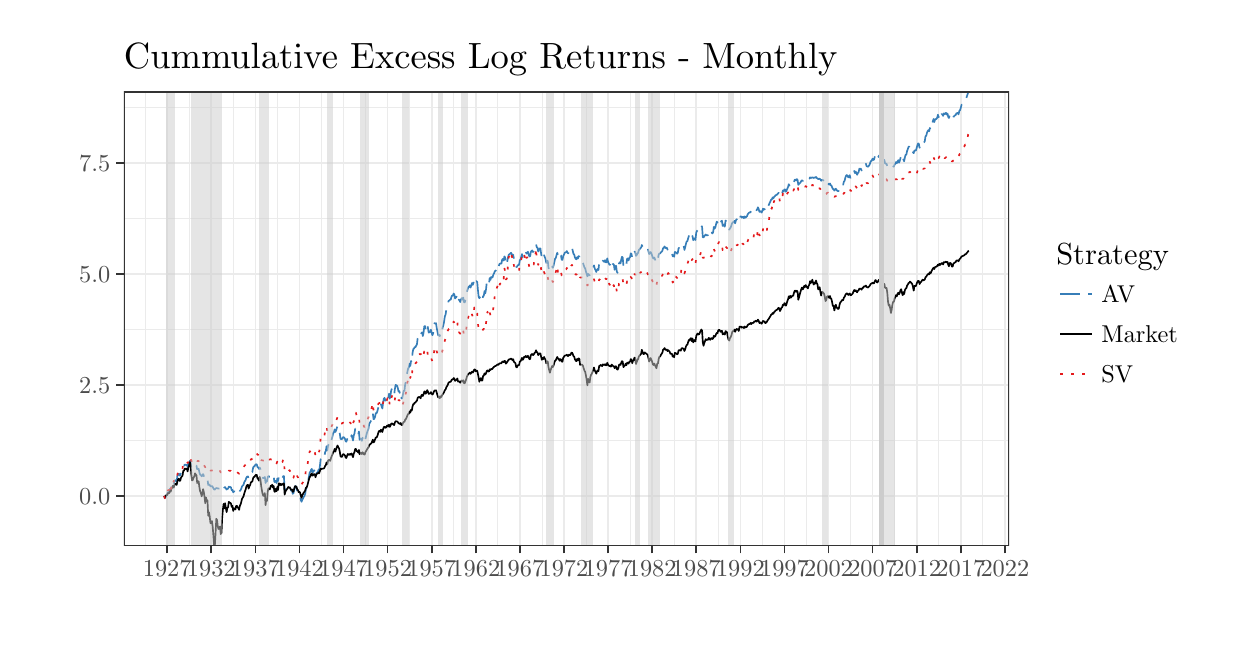
\begin{tikzpicture}[x=1pt,y=1pt]
\definecolor{fillColor}{RGB}{255,255,255}
\path[use as bounding box,fill=fillColor,fill opacity=0.00] (0,0) rectangle (426.79,216.81);
\begin{scope}
\path[clip] (  0.00,  0.00) rectangle (426.79,216.81);
\definecolor{drawColor}{RGB}{255,255,255}
\definecolor{fillColor}{RGB}{255,255,255}

\path[draw=drawColor,line width= 0.6pt,line join=round,line cap=round,fill=fillColor] (  0.00,  0.00) rectangle (426.79,216.81);
\end{scope}
\begin{scope}
\path[clip] ( 34.77, 29.59) rectangle (354.63,193.67);
\definecolor{fillColor}{RGB}{255,255,255}

\path[fill=fillColor] ( 34.77, 29.59) rectangle (354.63,193.67);
\definecolor{drawColor}{gray}{0.92}

\path[draw=drawColor,line width= 0.3pt,line join=round] ( 34.77, 67.61) --
	(354.63, 67.61);

\path[draw=drawColor,line width= 0.3pt,line join=round] ( 34.77,107.75) --
	(354.63,107.75);

\path[draw=drawColor,line width= 0.3pt,line join=round] ( 34.77,147.89) --
	(354.63,147.89);

\path[draw=drawColor,line width= 0.3pt,line join=round] ( 34.77,188.02) --
	(354.63,188.02);

\path[draw=drawColor,line width= 0.3pt,line join=round] ( 42.44, 29.59) --
	( 42.44,193.67);

\path[draw=drawColor,line width= 0.3pt,line join=round] ( 58.37, 29.59) --
	( 58.37,193.67);

\path[draw=drawColor,line width= 0.3pt,line join=round] ( 74.31, 29.59) --
	( 74.31,193.67);

\path[draw=drawColor,line width= 0.3pt,line join=round] ( 90.24, 29.59) --
	( 90.24,193.67);

\path[draw=drawColor,line width= 0.3pt,line join=round] (106.17, 29.59) --
	(106.17,193.67);

\path[draw=drawColor,line width= 0.3pt,line join=round] (122.10, 29.59) --
	(122.10,193.67);

\path[draw=drawColor,line width= 0.3pt,line join=round] (138.04, 29.59) --
	(138.04,193.67);

\path[draw=drawColor,line width= 0.3pt,line join=round] (153.97, 29.59) --
	(153.97,193.67);

\path[draw=drawColor,line width= 0.3pt,line join=round] (169.90, 29.59) --
	(169.90,193.67);

\path[draw=drawColor,line width= 0.3pt,line join=round] (185.83, 29.59) --
	(185.83,193.67);

\path[draw=drawColor,line width= 0.3pt,line join=round] (201.77, 29.59) --
	(201.77,193.67);

\path[draw=drawColor,line width= 0.3pt,line join=round] (217.70, 29.59) --
	(217.70,193.67);

\path[draw=drawColor,line width= 0.3pt,line join=round] (233.63, 29.59) --
	(233.63,193.67);

\path[draw=drawColor,line width= 0.3pt,line join=round] (249.57, 29.59) --
	(249.57,193.67);

\path[draw=drawColor,line width= 0.3pt,line join=round] (265.50, 29.59) --
	(265.50,193.67);

\path[draw=drawColor,line width= 0.3pt,line join=round] (281.44, 29.59) --
	(281.44,193.67);

\path[draw=drawColor,line width= 0.3pt,line join=round] (297.37, 29.59) --
	(297.37,193.67);

\path[draw=drawColor,line width= 0.3pt,line join=round] (313.30, 29.59) --
	(313.30,193.67);

\path[draw=drawColor,line width= 0.3pt,line join=round] (329.23, 29.59) --
	(329.23,193.67);

\path[draw=drawColor,line width= 0.3pt,line join=round] (345.17, 29.59) --
	(345.17,193.67);

\path[draw=drawColor,line width= 0.6pt,line join=round] ( 34.77, 47.54) --
	(354.63, 47.54);

\path[draw=drawColor,line width= 0.6pt,line join=round] ( 34.77, 87.68) --
	(354.63, 87.68);

\path[draw=drawColor,line width= 0.6pt,line join=round] ( 34.77,127.82) --
	(354.63,127.82);

\path[draw=drawColor,line width= 0.6pt,line join=round] ( 34.77,167.95) --
	(354.63,167.95);

\path[draw=drawColor,line width= 0.6pt,line join=round] ( 50.41, 29.59) --
	( 50.41,193.67);

\path[draw=drawColor,line width= 0.6pt,line join=round] ( 66.34, 29.59) --
	( 66.34,193.67);

\path[draw=drawColor,line width= 0.6pt,line join=round] ( 82.28, 29.59) --
	( 82.28,193.67);

\path[draw=drawColor,line width= 0.6pt,line join=round] ( 98.21, 29.59) --
	( 98.21,193.67);

\path[draw=drawColor,line width= 0.6pt,line join=round] (114.14, 29.59) --
	(114.14,193.67);

\path[draw=drawColor,line width= 0.6pt,line join=round] (130.07, 29.59) --
	(130.07,193.67);

\path[draw=drawColor,line width= 0.6pt,line join=round] (146.01, 29.59) --
	(146.01,193.67);

\path[draw=drawColor,line width= 0.6pt,line join=round] (161.94, 29.59) --
	(161.94,193.67);

\path[draw=drawColor,line width= 0.6pt,line join=round] (177.87, 29.59) --
	(177.87,193.67);

\path[draw=drawColor,line width= 0.6pt,line join=round] (193.80, 29.59) --
	(193.80,193.67);

\path[draw=drawColor,line width= 0.6pt,line join=round] (209.74, 29.59) --
	(209.74,193.67);

\path[draw=drawColor,line width= 0.6pt,line join=round] (225.67, 29.59) --
	(225.67,193.67);

\path[draw=drawColor,line width= 0.6pt,line join=round] (241.60, 29.59) --
	(241.60,193.67);

\path[draw=drawColor,line width= 0.6pt,line join=round] (257.53, 29.59) --
	(257.53,193.67);

\path[draw=drawColor,line width= 0.6pt,line join=round] (273.47, 29.59) --
	(273.47,193.67);

\path[draw=drawColor,line width= 0.6pt,line join=round] (289.40, 29.59) --
	(289.40,193.67);

\path[draw=drawColor,line width= 0.6pt,line join=round] (305.33, 29.59) --
	(305.33,193.67);

\path[draw=drawColor,line width= 0.6pt,line join=round] (321.26, 29.59) --
	(321.26,193.67);

\path[draw=drawColor,line width= 0.6pt,line join=round] (337.20, 29.59) --
	(337.20,193.67);

\path[draw=drawColor,line width= 0.6pt,line join=round] (353.13, 29.59) --
	(353.13,193.67);
\definecolor{drawColor}{RGB}{55,126,184}

\path[draw=drawColor,line width= 0.6pt,dash pattern=on 7pt off 3pt ,line join=round] ( 49.31, 47.61) --
	( 49.58, 46.82) --
	( 49.84, 47.22) --
	( 50.11, 47.85) --
	( 50.37, 47.83) --
	( 50.64, 48.93) --
	( 50.91, 48.96) --
	( 51.16, 49.05) --
	( 51.43, 50.24) --
	( 51.69, 49.70) --
	( 51.96, 51.16) --
	( 52.22, 51.62) --
	( 52.49, 52.47) --
	( 52.76, 51.59) --
	( 53.02, 52.85) --
	( 53.29, 53.30) --
	( 53.56, 53.18) --
	( 53.83, 52.79) --
	( 54.10, 54.88) --
	( 54.35, 55.42) --
	( 54.62, 55.62) --
	( 54.88, 55.00) --
	( 55.15, 55.05) --
	( 55.41, 56.24) --
	( 55.68, 56.69) --
	( 55.95, 56.95) --
	( 56.22, 58.52) --
	( 56.49, 58.53) --
	( 56.75, 58.89) --
	( 57.02, 58.88) --
	( 57.29, 58.74) --
	( 57.53, 58.87) --
	( 57.80, 58.09) --
	( 58.07, 58.97) --
	( 58.34, 59.42) --
	( 58.60, 60.28) --
	( 58.87, 59.80) --
	( 59.14, 57.72) --
	( 59.40, 57.59) --
	( 59.67, 57.61) --
	( 59.93, 57.83) --
	( 60.20, 58.08) --
	( 60.47, 58.99) --
	( 60.72, 58.73) --
	( 60.99, 58.52) --
	( 61.25, 57.25) --
	( 61.52, 57.41) --
	( 61.78, 57.42) --
	( 62.05, 56.09) --
	( 62.32, 55.27) --
	( 62.59, 55.15) --
	( 62.86, 54.71) --
	( 63.12, 54.98) --
	( 63.39, 55.50) --
	( 63.66, 54.82) --
	( 63.90, 54.13) --
	( 64.17, 53.56) --
	( 64.43, 54.02) --
	( 64.71, 53.84) --
	( 64.97, 53.86) --
	( 65.24, 51.55) --
	( 65.51, 51.74) --
	( 65.77, 51.62) --
	( 66.04, 51.07) --
	( 66.30, 51.05) --
	( 66.57, 51.17) --
	( 66.84, 50.91) --
	( 67.10, 50.40) --
	( 67.37, 49.92) --
	( 67.63, 49.91) --
	( 67.90, 50.28) --
	( 68.16, 50.45) --
	( 68.43, 50.41) --
	( 68.70, 50.30) --
	( 68.96, 50.23) --
	( 69.23, 50.34) --
	( 69.49, 50.36) --
	( 69.77, 49.49) --
	( 70.04, 49.61) --
	( 70.28, 50.13) --
	( 70.55, 50.50) --
	( 70.81, 50.85) --
	( 71.08, 50.60) --
	( 71.34, 50.80) --
	( 71.61, 50.28) --
	( 71.89, 49.92) --
	( 72.15, 50.15) --
	( 72.42, 50.24) --
	( 72.68, 50.96) --
	( 72.95, 50.81) --
	( 73.22, 50.84) --
	( 73.46, 50.69) --
	( 73.73, 49.63) --
	( 74.00, 49.80) --
	( 74.27, 48.93) --
	( 74.53, 49.21) --
	( 74.80, 49.20) --
	( 75.07, 49.04) --
	( 75.33, 49.68) --
	( 75.60, 49.71) --
	( 75.86, 49.39) --
	( 76.13, 49.14) --
	( 76.40, 48.71) --
	( 76.65, 49.37) --
	( 76.92, 49.70) --
	( 77.18, 50.21) --
	( 77.45, 51.01) --
	( 77.71, 51.36) --
	( 77.98, 51.58) --
	( 78.25, 52.52) --
	( 78.52, 52.96) --
	( 78.79, 53.46) --
	( 79.05, 54.26) --
	( 79.32, 54.56) --
	( 79.59, 54.67) --
	( 79.84, 53.85) --
	( 80.11, 54.34) --
	( 80.37, 54.65) --
	( 80.64, 55.89) --
	( 80.91, 56.08) --
	( 81.18, 56.28) --
	( 81.45, 57.75) --
	( 81.71, 58.28) --
	( 81.98, 58.31) --
	( 82.24, 58.84) --
	( 82.51, 59.05) --
	( 82.78, 59.00) --
	( 83.03, 58.02) --
	( 83.30, 57.95) --
	( 83.56, 57.38) --
	( 83.83, 57.85) --
	( 84.09, 57.29) --
	( 84.36, 54.72) --
	( 84.63, 54.33) --
	( 84.89, 54.18) --
	( 85.16, 54.07) --
	( 85.43, 54.12) --
	( 85.70, 54.46) --
	( 85.97, 52.29) --
	( 86.21, 52.98) --
	( 86.48, 52.83) --
	( 86.74, 54.36) --
	( 87.01, 54.76) --
	( 87.28, 54.55) --
	( 87.55, 54.58) --
	( 87.82, 54.88) --
	( 88.08, 54.71) --
	( 88.35, 55.18) --
	( 88.61, 54.50) --
	( 88.88, 54.77) --
	( 89.15, 52.65) --
	( 89.40, 52.63) --
	( 89.67, 53.05) --
	( 89.93, 52.27) --
	( 90.20, 53.89) --
	( 90.46, 52.98) --
	( 90.73, 54.29) --
	( 91.00, 54.27) --
	( 91.26, 53.56) --
	( 91.53, 54.28) --
	( 91.79, 53.74) --
	( 92.06, 54.09) --
	( 92.34, 54.76) --
	( 92.59, 54.78) --
	( 92.86, 49.55) --
	( 93.12, 49.76) --
	( 93.39, 49.94) --
	( 93.65, 50.40) --
	( 93.92, 50.70) --
	( 94.19, 51.10) --
	( 94.46, 50.78) --
	( 94.73, 50.84) --
	( 94.99, 49.74) --
	( 95.26, 49.45) --
	( 95.53, 49.62) --
	( 95.77, 48.37) --
	( 96.04, 48.60) --
	( 96.30, 49.72) --
	( 96.58, 51.12) --
	( 96.84, 51.09) --
	( 97.11, 50.84) --
	( 97.38, 49.41) --
	( 97.64, 48.95) --
	( 97.91, 47.86) --
	( 98.17, 47.92) --
	( 98.44, 47.61) --
	( 98.71, 46.10) --
	( 98.96, 45.49) --
	( 99.23, 46.26) --
	( 99.49, 46.66) --
	( 99.76, 47.29) --
	(100.02, 47.63) --
	(100.29, 48.39) --
	(100.56, 50.36) --
	(100.82, 50.37) --
	(101.09, 51.59) --
	(101.36, 53.07) --
	(101.63, 54.54) --
	(101.90, 56.12) --
	(102.14, 56.25) --
	(102.41, 57.06) --
	(102.67, 57.38) --
	(102.94, 56.15) --
	(103.21, 56.38) --
	(103.48, 56.88) --
	(103.75, 56.48) --
	(104.01, 54.54) --
	(104.28, 55.63) --
	(104.54, 56.03) --
	(104.81, 56.14) --
	(105.08, 57.05) --
	(105.33, 56.52) --
	(105.60, 58.48) --
	(105.87, 60.85) --
	(106.14, 60.42) --
	(106.40, 60.84) --
	(106.67, 60.85) --
	(106.94, 60.90) --
	(107.20, 61.62) --
	(107.47, 63.33) --
	(107.73, 63.89) --
	(108.00, 65.58) --
	(108.27, 64.04) --
	(108.52, 65.75) --
	(108.79, 66.26) --
	(109.05, 66.38) --
	(109.32, 65.82) --
	(109.58, 67.14) --
	(109.85, 68.06) --
	(110.12, 69.05) --
	(110.39, 70.30) --
	(110.66, 70.54) --
	(110.92, 71.62) --
	(111.19, 70.71) --
	(111.46, 71.32) --
	(111.70, 72.09) --
	(111.97, 72.94) --
	(112.24, 72.12) --
	(112.51, 71.54) --
	(112.77, 70.26) --
	(113.04, 68.22) --
	(113.31, 68.16) --
	(113.57, 68.16) --
	(113.84, 68.72) --
	(114.10, 68.86) --
	(114.37, 68.67) --
	(114.64, 68.26) --
	(114.89, 67.37) --
	(115.16, 67.19) --
	(115.42, 68.04) --
	(115.69, 68.86) --
	(115.95, 68.51) --
	(116.22, 68.37) --
	(116.49, 68.99) --
	(116.75, 68.47) --
	(117.03, 69.56) --
	(117.29, 68.68) --
	(117.56, 67.64) --
	(117.83, 69.45) --
	(118.08, 70.14) --
	(118.35, 71.88) --
	(118.61, 71.86) --
	(118.88, 70.54) --
	(119.15, 70.60) --
	(119.42, 69.67) --
	(119.69, 70.88) --
	(119.95, 67.88) --
	(120.22, 68.24) --
	(120.48, 68.31) --
	(120.75, 67.52) --
	(121.02, 68.61) --
	(121.27, 68.08) --
	(121.54, 66.92) --
	(121.80, 66.96) --
	(122.07, 68.24) --
	(122.33, 69.40) --
	(122.60, 70.41) --
	(122.87, 71.19) --
	(123.13, 71.83) --
	(123.40, 73.55) --
	(123.66, 74.07) --
	(123.93, 74.50) --
	(124.21, 75.03) --
	(124.45, 76.32) --
	(124.72, 77.55) --
	(124.98, 75.32) --
	(125.25, 75.49) --
	(125.51, 76.14) --
	(125.78, 77.49) --
	(126.05, 77.42) --
	(126.32, 78.09) --
	(126.59, 79.12) --
	(126.85, 80.02) --
	(127.12, 80.29) --
	(127.39, 79.45) --
	(127.63, 80.78) --
	(127.90, 79.97) --
	(128.17, 79.21) --
	(128.44, 81.48) --
	(128.70, 82.75) --
	(128.97, 83.03) --
	(129.24, 82.03) --
	(129.50, 82.14) --
	(129.77, 83.23) --
	(130.03, 83.94) --
	(130.30, 82.95) --
	(130.57, 84.51) --
	(130.83, 82.74) --
	(131.10, 83.94) --
	(131.36, 85.76) --
	(131.63, 86.38) --
	(131.89, 85.92) --
	(132.16, 84.50) --
	(132.43, 84.15) --
	(132.69, 86.28) --
	(132.96, 87.72) --
	(133.23, 87.58) --
	(133.50, 87.40) --
	(133.77, 86.53) --
	(134.01, 85.34) --
	(134.28, 85.51) --
	(134.54, 84.53) --
	(134.81, 85.32) --
	(135.08, 82.82) --
	(135.35, 82.90) --
	(135.62, 84.38) --
	(135.88, 85.66) --
	(136.15, 85.62) --
	(136.41, 87.98) --
	(136.68, 88.77) --
	(136.95, 90.64) --
	(137.20, 92.43) --
	(137.47, 93.63) --
	(137.73, 94.10) --
	(138.00, 95.41) --
	(138.26, 94.56) --
	(138.53, 96.38) --
	(138.80, 95.66) --
	(139.06, 99.20) --
	(139.33,100.66) --
	(139.60,100.84) --
	(139.87,101.41) --
	(140.14,101.34) --
	(140.38,101.92) --
	(140.65,102.33) --
	(140.91,104.48) --
	(141.18,105.12) --
	(141.44,105.19) --
	(141.72,105.09) --
	(141.99,104.76) --
	(142.25,106.36) --
	(142.52,106.71) --
	(142.78,105.37) --
	(143.05,106.61) --
	(143.32,108.90) --
	(143.57,109.00) --
	(143.84,107.55) --
	(144.11,108.36) --
	(144.38,109.51) --
	(144.64,108.29) --
	(144.91,106.60) --
	(145.18,106.82) --
	(145.44,106.90) --
	(145.71,107.69) --
	(145.97,106.48) --
	(146.24,105.69) --
	(146.51,106.36) --
	(146.76,108.65) --
	(147.03,110.06) --
	(147.29,109.80) --
	(147.56,110.02) --
	(147.82,108.19) --
	(148.09,106.84) --
	(148.36,105.63) --
	(148.62,105.86) --
	(148.90,105.34) --
	(149.16,106.50) --
	(149.43,106.04) --
	(149.70,107.23) --
	(149.94,108.43) --
	(150.21,109.29) --
	(150.47,110.57) --
	(150.74,112.51) --
	(151.01,113.13) --
	(151.28,115.01) --
	(151.55,116.03) --
	(151.81,116.80) --
	(152.08,118.04) --
	(152.34,118.22) --
	(152.61,118.49) --
	(152.88,118.57) --
	(153.13,119.56) --
	(153.40,120.03) --
	(153.66,119.99) --
	(153.93,120.73) --
	(154.19,120.33) --
	(154.46,118.96) --
	(154.73,119.26) --
	(154.99,119.67) --
	(155.26,120.36) --
	(155.53,118.20) --
	(155.80,118.55) --
	(156.07,118.14) --
	(156.32,117.68) --
	(156.59,118.58) --
	(156.85,119.07) --
	(157.12,118.54) --
	(157.38,119.27) --
	(157.65,117.65) --
	(157.92,117.51) --
	(158.19,118.54) --
	(158.46,119.87) --
	(158.72,121.42) --
	(158.99,122.27) --
	(159.26,123.10) --
	(159.50,123.20) --
	(159.77,123.67) --
	(160.04,122.87) --
	(160.31,123.75) --
	(160.57,124.54) --
	(160.84,123.89) --
	(161.11,124.65) --
	(161.37,125.95) --
	(161.64,125.92) --
	(161.90,124.75) --
	(162.17,125.21) --
	(162.44,124.92) --
	(162.69,122.08) --
	(162.96,119.51) --
	(163.22,119.06) --
	(163.49,119.57) --
	(163.75,119.96) --
	(164.02,118.43) --
	(164.29,118.43) --
	(164.56,119.74) --
	(164.83,119.98) --
	(165.09,121.63) --
	(165.36,120.81) --
	(165.63,122.33) --
	(165.87,124.63) --
	(166.14,125.34) --
	(166.40,124.42) --
	(166.68,124.21) --
	(166.94,126.34) --
	(167.21,125.66) --
	(167.48,126.71) --
	(167.74,126.47) --
	(168.01,126.71) --
	(168.27,127.59) --
	(168.54,128.06) --
	(168.81,128.82) --
	(169.07,128.91) --
	(169.34,129.44) --
	(169.60,129.96) --
	(169.87,130.66) --
	(170.13,129.98) --
	(170.40,131.26) --
	(170.67,131.56) --
	(170.93,131.57) --
	(171.20,131.61) --
	(171.47,133.04) --
	(171.74,133.24) --
	(172.01,132.66) --
	(172.25,134.17) --
	(172.52,133.76) --
	(172.78,131.04) --
	(173.05,131.35) --
	(173.31,132.45) --
	(173.59,133.87) --
	(173.86,134.84) --
	(174.12,134.84) --
	(174.39,135.22) --
	(174.65,135.45) --
	(174.92,135.07) --
	(175.19,134.28) --
	(175.43,134.74) --
	(175.71,133.22) --
	(175.97,133.01) --
	(176.24,132.59) --
	(176.50,130.41) --
	(176.77,130.29) --
	(177.04,130.88) --
	(177.30,131.04) --
	(177.57,131.08) --
	(177.83,132.84) --
	(178.10,132.99) --
	(178.37,134.11) --
	(178.62,134.98) --
	(178.89,133.89) --
	(179.15,134.44) --
	(179.42,135.35) --
	(179.68,135.15) --
	(179.95,136.00) --
	(180.22,135.18) --
	(180.49,135.29) --
	(180.76,135.85) --
	(181.02,134.85) --
	(181.29,134.14) --
	(181.56,134.17) --
	(181.81,135.77) --
	(182.08,136.14) --
	(182.34,136.30) --
	(182.61,135.74) --
	(182.88,136.02) --
	(183.15,137.13) --
	(183.42,137.26) --
	(183.68,138.63) --
	(183.95,137.52) --
	(184.21,137.25) --
	(184.48,135.93) --
	(184.75,136.64) --
	(185.00,137.05) --
	(185.27,137.06) --
	(185.53,135.14) --
	(185.80,133.51) --
	(186.06,134.14) --
	(186.33,133.59) --
	(186.60,134.57) --
	(186.86,133.90) --
	(187.13,133.22) --
	(187.40,131.81) --
	(187.67,132.62) --
	(187.94,132.45) --
	(188.18,130.14) --
	(188.45,128.96) --
	(188.71,128.63) --
	(188.98,129.33) --
	(189.25,129.86) --
	(189.52,130.44) --
	(189.79,130.04) --
	(190.05,130.89) --
	(190.32,132.17) --
	(190.58,133.33) --
	(190.85,133.62) --
	(191.12,134.70) --
	(191.37,135.47) --
	(191.64,134.49) --
	(191.90,134.50) --
	(192.17,133.49) --
	(192.43,134.62) --
	(192.70,134.49) --
	(192.97,132.99) --
	(193.23,132.86) --
	(193.50,134.26) --
	(193.76,134.73) --
	(194.03,135.43) --
	(194.31,135.60) --
	(194.56,135.67) --
	(194.83,136.09) --
	(195.09,135.48) --
	(195.36,135.26) --
	(195.62,136.06) --
	(195.89,135.84) --
	(196.16,136.02) --
	(196.43,137.09) --
	(196.70,137.26) --
	(196.96,136.20) --
	(197.23,135.05) --
	(197.50,134.82) --
	(197.74,133.79) --
	(198.01,133.28) --
	(198.27,133.12) --
	(198.55,133.88) --
	(198.81,133.38) --
	(199.08,134.25) --
	(199.35,134.13) --
	(199.61,132.21) --
	(199.88,132.25) --
	(200.14,132.25) --
	(200.41,132.21) --
	(200.68,131.76) --
	(200.93,130.92) --
	(201.20,130.15) --
	(201.46,129.79) --
	(201.73,128.67) --
	(201.99,127.90) --
	(202.26,126.93) --
	(202.53,127.81) --
	(202.79,127.59) --
	(203.06,127.31) --
	(203.33,128.46) --
	(203.60,128.84) --
	(203.87,129.12) --
	(204.11,129.64) --
	(204.38,130.25) --
	(204.64,130.90) --
	(204.91,129.74) --
	(205.18,129.20) --
	(205.45,128.54) --
	(205.72,129.27) --
	(205.98,129.65) --
	(206.25,129.24) --
	(206.51,131.67) --
	(206.78,131.71) --
	(207.05,132.14) --
	(207.30,131.87) --
	(207.58,131.54) --
	(207.84,132.62) --
	(208.11,132.37) --
	(208.37,132.18) --
	(208.64,132.79) --
	(208.91,132.00) --
	(209.17,132.03) --
	(209.44,133.45) --
	(209.70,132.24) --
	(209.97,131.63) --
	(210.24,131.13) --
	(210.49,131.18) --
	(210.76,130.75) --
	(211.02,132.52) --
	(211.29,131.89) --
	(211.55,131.30) --
	(211.82,131.21) --
	(212.09,129.32) --
	(212.36,130.63) --
	(212.63,130.72) --
	(212.89,128.64) --
	(213.16,128.20) --
	(213.43,129.31) --
	(213.67,131.61) --
	(213.94,132.02) --
	(214.21,131.64) --
	(214.48,132.97) --
	(214.74,134.01) --
	(215.01,133.75) --
	(215.28,130.67) --
	(215.54,131.17) --
	(215.81,131.33) --
	(216.07,132.25) --
	(216.34,131.39) --
	(216.61,133.35) --
	(216.86,133.39) --
	(217.13,132.70) --
	(217.39,133.63) --
	(217.66,133.81) --
	(217.92,135.24) --
	(218.19,135.07) --
	(218.46,133.48) --
	(218.72,134.18) --
	(219.00,134.53) --
	(219.26,135.85) --
	(219.53,135.76) --
	(219.80,134.34) --
	(220.05,134.63) --
	(220.32,135.11) --
	(220.58,135.48) --
	(220.85,136.47) --
	(221.12,136.75) --
	(221.39,137.14) --
	(221.66,137.29) --
	(221.92,138.27) --
	(222.19,137.71) --
	(222.45,137.21) --
	(222.72,137.24) --
	(222.99,137.78) --
	(223.24,137.54) --
	(223.51,137.56) --
	(223.77,137.25) --
	(224.04,137.09) --
	(224.30,136.06) --
	(224.57,134.99) --
	(224.84,135.42) --
	(225.10,135.72) --
	(225.37,135.25) --
	(225.63,134.49) --
	(225.90,133.69) --
	(226.18,133.39) --
	(226.42,133.75) --
	(226.69,133.11) --
	(226.95,132.31) --
	(227.22,131.87) --
	(227.48,133.38) --
	(227.75,133.42) --
	(228.02,134.88) --
	(228.29,135.18) --
	(228.56,135.26) --
	(228.82,135.62) --
	(229.09,135.84) --
	(229.36,136.24) --
	(229.60,137.13) --
	(229.87,137.25) --
	(230.14,137.75) --
	(230.41,137.23) --
	(230.67,137.18) --
	(230.94,137.31) --
	(231.21,136.62) --
	(231.47,136.97) --
	(231.74,136.62) --
	(232.00,136.19) --
	(232.27,135.37) --
	(232.54,135.44) --
	(232.80,135.37) --
	(233.07,134.20) --
	(233.33,134.48) --
	(233.60,134.02) --
	(233.86,135.75) --
	(234.13,135.66) --
	(234.40,135.47) --
	(234.66,135.13) --
	(234.93,135.48) --
	(235.20,137.09) --
	(235.47,137.28) --
	(235.74,137.08) --
	(235.98,136.91) --
	(236.25,138.19) --
	(236.51,138.41) --
	(236.78,138.23) --
	(237.05,138.00) --
	(237.32,136.49) --
	(237.59,137.49) --
	(237.85,138.63) --
	(238.12,139.59) --
	(238.38,139.66) --
	(238.65,140.65) --
	(238.92,141.54) --
	(239.17,141.32) --
	(239.44,141.91) --
	(239.70,142.08) --
	(239.97,140.79) --
	(240.23,141.55) --
	(240.50,140.00) --
	(240.77,140.48) --
	(241.03,140.67) --
	(241.30,140.09) --
	(241.57,142.71) --
	(241.84,143.33) --
	(242.11,143.67) --
	(242.35,143.33) --
	(242.62,143.34) --
	(242.88,143.84) --
	(243.15,144.66) --
	(243.41,145.30) --
	(243.69,144.86) --
	(243.96,141.10) --
	(244.22,141.01) --
	(244.49,141.46) --
	(244.75,141.76) --
	(245.02,142.07) --
	(245.29,141.74) --
	(245.54,141.84) --
	(245.81,141.78) --
	(246.08,142.64) --
	(246.35,142.41) --
	(246.61,141.64) --
	(246.88,142.44) --
	(247.15,142.75) --
	(247.41,142.45) --
	(247.68,142.84) --
	(247.94,144.82) --
	(248.21,144.20) --
	(248.48,144.66) --
	(248.73,145.69) --
	(249.00,146.72) --
	(249.26,146.40) --
	(249.53,147.64) --
	(249.79,148.02) --
	(250.06,147.84) --
	(250.33,146.66) --
	(250.59,146.77) --
	(250.87,147.06) --
	(251.13,145.15) --
	(251.40,145.28) --
	(251.67,145.73) --
	(251.91,144.89) --
	(252.18,147.13) --
	(252.44,146.86) --
	(252.71,146.48) --
	(252.98,144.61) --
	(253.25,144.11) --
	(253.52,143.84) --
	(253.78,144.32) --
	(254.05,144.63) --
	(254.31,145.45) --
	(254.58,146.22) --
	(254.85,146.52) --
	(255.10,146.49) --
	(255.37,147.01) --
	(255.63,146.11) --
	(255.90,147.12) --
	(256.16,147.59) --
	(256.43,147.31) --
	(256.70,147.66) --
	(256.96,146.92) --
	(257.23,148.61) --
	(257.50,148.53) --
	(257.77,148.65) --
	(258.04,148.15) --
	(258.29,148.42) --
	(258.56,148.47) --
	(258.82,147.94) --
	(259.09,148.63) --
	(259.35,148.14) --
	(259.62,148.42) --
	(259.89,148.61) --
	(260.16,149.33) --
	(260.43,149.70) --
	(260.69,149.94) --
	(260.96,149.99) --
	(261.23,150.32) --
	(261.47,149.81) --
	(261.74,150.14) --
	(262.01,150.20) --
	(262.28,150.14) --
	(262.54,150.91) --
	(262.81,150.87) --
	(263.08,151.19) --
	(263.34,150.84) --
	(263.61,151.15) --
	(263.87,151.89) --
	(264.14,151.34) --
	(264.41,150.27) --
	(264.66,150.40) --
	(264.93,150.49) --
	(265.19,149.98) --
	(265.46,150.52) --
	(265.72,151.44) --
	(265.99,151.00) --
	(266.26,151.28) --
	(266.53,150.39) --
	(266.80,150.58) --
	(267.06,150.95) --
	(267.33,151.75) --
	(267.60,152.39) --
	(267.84,152.86) --
	(268.11,153.51) --
	(268.38,154.01) --
	(268.65,154.69) --
	(268.91,154.76) --
	(269.18,155.47) --
	(269.45,155.13) --
	(269.71,155.68) --
	(269.98,155.85) --
	(270.24,156.24) --
	(270.51,156.37) --
	(270.78,156.48) --
	(271.04,156.76) --
	(271.31,157.12) --
	(271.57,156.88) --
	(271.84,155.55) --
	(272.10,155.86) --
	(272.37,156.75) --
	(272.64,156.95) --
	(272.90,157.98) --
	(273.17,157.67) --
	(273.44,158.39) --
	(273.71,158.31) --
	(273.98,157.52) --
	(274.22,158.00) --
	(274.49,158.64) --
	(274.75,159.21) --
	(275.02,160.24) --
	(275.28,159.76) --
	(275.56,160.49) --
	(275.83,159.96) --
	(276.09,160.11) --
	(276.36,160.29) --
	(276.62,160.30) --
	(276.89,161.01) --
	(277.16,161.83) --
	(277.40,161.93) --
	(277.68,161.62) --
	(277.94,162.08) --
	(278.21,161.75) --
	(278.47,160.00) --
	(278.74,160.34) --
	(279.01,160.63) --
	(279.27,160.86) --
	(279.54,161.43) --
	(279.80,161.69) --
	(280.07,161.43) --
	(280.34,161.69) --
	(280.59,162.01) --
	(280.86,161.90) --
	(281.12,162.22) --
	(281.39,161.97) --
	(281.65,161.83) --
	(281.92,161.61) --
	(282.19,162.07) --
	(282.46,162.24) --
	(282.73,162.70) --
	(282.99,162.49) --
	(283.26,162.57) --
	(283.53,162.76) --
	(283.78,162.59) --
	(284.05,162.50) --
	(284.31,162.67) --
	(284.58,162.57) --
	(284.85,162.87) --
	(285.12,162.51) --
	(285.39,162.36) --
	(285.65,162.10) --
	(285.92,162.15) --
	(286.18,162.25) --
	(286.45,161.98) --
	(286.72,161.49) --
	(286.97,161.78) --
	(287.24,161.80) --
	(287.50,161.62) --
	(287.77,161.41) --
	(288.03,160.93) --
	(288.30,159.80) --
	(288.57,159.93) --
	(288.83,160.36) --
	(289.10,160.53) --
	(289.37,160.32) --
	(289.64,160.08) --
	(289.91,160.52) --
	(290.15,159.89) --
	(290.42,159.77) --
	(290.68,159.17) --
	(290.95,158.48) --
	(291.22,158.50) --
	(291.49,157.92) --
	(291.76,158.40) --
	(292.02,158.61) --
	(292.29,158.19) --
	(292.55,157.86) --
	(292.82,157.71) --
	(293.09,157.86) --
	(293.34,158.58) --
	(293.61,159.38) --
	(293.87,159.60) --
	(294.14,159.96) --
	(294.40,160.33) --
	(294.67,160.08) --
	(294.94,161.19) --
	(295.20,161.48) --
	(295.47,162.65) --
	(295.73,163.28) --
	(296.00,163.55) --
	(296.28,163.24) --
	(296.53,162.72) --
	(296.80,162.97) --
	(297.06,163.49) --
	(297.33,162.29) --
	(297.59,162.33) --
	(297.86,162.80) --
	(298.13,163.24) --
	(298.40,164.15) --
	(298.67,165.04) --
	(298.93,164.24) --
	(299.20,164.80) --
	(299.47,164.29) --
	(299.71,163.63) --
	(299.98,164.28) --
	(300.25,164.56) --
	(300.52,165.86) --
	(300.78,165.63) --
	(301.05,165.87) --
	(301.32,165.21) --
	(301.58,165.78) --
	(301.85,165.80) --
	(302.11,167.02) --
	(302.38,166.92) --
	(302.65,167.34) --
	(302.90,167.60) --
	(303.17,166.72) --
	(303.43,166.65) --
	(303.70,166.55) --
	(303.96,166.91) --
	(304.23,167.30) --
	(304.50,168.17) --
	(304.76,168.64) --
	(305.03,168.82) --
	(305.30,169.47) --
	(305.57,168.99) --
	(305.84,169.22) --
	(306.08,170.14) --
	(306.35,171.21) --
	(306.61,170.66) --
	(306.88,169.70) --
	(307.15,169.83) --
	(307.42,170.16) --
	(307.69,170.64) --
	(307.95,169.90) --
	(308.22,169.84) --
	(308.48,168.79) --
	(308.75,168.62) --
	(309.02,168.49) --
	(309.27,168.80) --
	(309.55,169.01) --
	(309.81,167.81) --
	(310.08,167.64) --
	(310.34,167.68) --
	(310.61,166.76) --
	(310.88,166.32) --
	(311.14,166.23) --
	(311.41,166.26) --
	(311.67,166.04) --
	(311.94,165.70) --
	(312.21,166.08) --
	(312.46,166.33) --
	(312.73,166.60) --
	(312.99,166.58) --
	(313.26,167.35) --
	(313.52,167.65) --
	(313.79,168.25) --
	(314.06,167.82) --
	(314.33,168.40) --
	(314.60,168.93) --
	(314.86,168.03) --
	(315.13,168.63) --
	(315.40,169.77) --
	(315.64,170.39) --
	(315.91,168.90) --
	(316.18,168.47) --
	(316.45,169.18) --
	(316.71,168.53) --
	(316.98,170.00) --
	(317.25,170.84) --
	(317.51,170.95) --
	(317.78,172.29) --
	(318.04,172.93) --
	(318.31,173.79) --
	(318.58,173.87) --
	(318.83,174.39) --
	(319.10,173.95) --
	(319.36,173.45) --
	(319.63,173.00) --
	(319.89,171.81) --
	(320.16,171.46) --
	(320.43,172.43) --
	(320.69,172.38) --
	(320.97,172.42) --
	(321.23,173.34) --
	(321.50,174.29) --
	(321.77,174.99) --
	(322.02,174.81) --
	(322.29,173.41) --
	(322.55,174.20) --
	(322.82,174.36) --
	(323.09,174.86) --
	(323.36,175.73) --
	(323.63,175.27) --
	(323.89,175.43) --
	(324.16,175.71) --
	(324.42,177.56) --
	(324.69,177.77) --
	(324.96,178.79) --
	(325.21,179.43) --
	(325.48,179.78) --
	(325.74,179.39) --
	(326.01,180.55) --
	(326.27,179.91) --
	(326.54,180.99) --
	(326.81,182.34) --
	(327.07,182.91) --
	(327.34,183.82) --
	(327.60,182.69) --
	(327.88,183.65) --
	(328.15,183.78) --
	(328.39,183.83) --
	(328.66,184.27) --
	(328.92,185.35) --
	(329.19,184.42) --
	(329.45,185.59) --
	(329.72,184.49) --
	(330.00,185.29) --
	(330.26,185.60) --
	(330.53,185.47) --
	(330.79,184.92) --
	(331.06,185.85) --
	(331.33,185.56) --
	(331.57,185.75) --
	(331.84,186.04) --
	(332.11,185.37) --
	(332.38,185.79) --
	(332.64,184.55) --
	(332.91,184.17) --
	(333.18,185.18) --
	(333.44,185.22) --
	(333.71,184.71) --
	(333.97,183.75) --
	(334.24,183.75) --
	(334.51,184.55) --
	(334.77,184.82) --
	(335.04,185.13) --
	(335.30,185.21) --
	(335.57,185.82) --
	(335.83,185.91) --
	(336.10,186.03) --
	(336.37,185.46) --
	(336.63,186.69) --
	(336.90,186.99) --
	(337.17,187.80) --
	(337.44,188.93) --
	(337.71,189.00) --
	(337.95,189.39) --
	(338.22,189.85) --
	(338.48,190.17) --
	(338.75,190.84) --
	(339.02,190.88) --
	(339.29,191.72) --
	(339.56,192.54) --
	(339.82,193.33) --
	(340.09,193.67);
\definecolor{drawColor}{RGB}{0,0,0}

\path[draw=drawColor,line width= 0.6pt,line join=round] ( 49.31, 47.60) --
	( 49.58, 47.09) --
	( 49.84, 47.50) --
	( 50.11, 47.91) --
	( 50.37, 47.90) --
	( 50.64, 48.57) --
	( 50.91, 48.59) --
	( 51.16, 48.66) --
	( 51.43, 49.52) --
	( 51.69, 49.14) --
	( 51.96, 50.25) --
	( 52.22, 50.57) --
	( 52.49, 51.30) --
	( 52.76, 50.59) --
	( 53.02, 51.62) --
	( 53.29, 51.96) --
	( 53.56, 51.87) --
	( 53.83, 51.60) --
	( 54.10, 52.95) --
	( 54.35, 53.59) --
	( 54.62, 53.82) --
	( 54.88, 53.04) --
	( 55.15, 53.14) --
	( 55.41, 54.18) --
	( 55.68, 54.63) --
	( 55.95, 54.88) --
	( 56.22, 56.68) --
	( 56.49, 56.70) --
	( 56.75, 57.49) --
	( 57.02, 57.47) --
	( 57.29, 57.29) --
	( 57.53, 57.50) --
	( 57.80, 56.46) --
	( 58.07, 57.95) --
	( 58.34, 58.60) --
	( 58.60, 59.83) --
	( 58.87, 58.95) --
	( 59.14, 55.37) --
	( 59.40, 53.19) --
	( 59.67, 53.38) --
	( 59.93, 54.23) --
	( 60.20, 54.62) --
	( 60.47, 55.75) --
	( 60.72, 55.37) --
	( 60.99, 55.09) --
	( 61.25, 52.26) --
	( 61.52, 52.87) --
	( 61.78, 52.89) --
	( 62.05, 50.72) --
	( 62.32, 49.25) --
	( 62.59, 48.76) --
	( 62.86, 47.44) --
	( 63.12, 48.42) --
	( 63.39, 50.06) --
	( 63.66, 49.00) --
	( 63.90, 47.30) --
	( 64.17, 44.97) --
	( 64.43, 47.06) --
	( 64.71, 45.95) --
	( 64.97, 45.98) --
	( 65.24, 40.43) --
	( 65.51, 41.69) --
	( 65.77, 40.20) --
	( 66.04, 37.85) --
	( 66.30, 37.66) --
	( 66.57, 38.54) --
	( 66.84, 36.62) --
	( 67.10, 33.41) --
	( 67.37, 29.67) --
	( 67.63, 29.59) --
	( 67.90, 34.28) --
	( 68.16, 39.35) --
	( 68.43, 38.88) --
	( 68.70, 36.59) --
	( 68.96, 35.62) --
	( 69.23, 36.33) --
	( 69.49, 36.48) --
	( 69.77, 33.81) --
	( 70.04, 34.33) --
	( 70.28, 39.67) --
	( 70.55, 42.77) --
	( 70.81, 44.76) --
	( 71.08, 43.13) --
	( 71.34, 44.97) --
	( 71.61, 43.17) --
	( 71.89, 41.76) --
	( 72.15, 43.28) --
	( 72.42, 43.57) --
	( 72.68, 45.48) --
	( 72.95, 45.08) --
	( 73.22, 45.15) --
	( 73.46, 44.85) --
	( 73.73, 43.64) --
	( 74.00, 44.04) --
	( 74.27, 42.18) --
	( 74.53, 43.07) --
	( 74.80, 43.03) --
	( 75.07, 42.72) --
	( 75.33, 43.98) --
	( 75.60, 44.04) --
	( 75.86, 43.49) --
	( 76.13, 43.17) --
	( 76.40, 42.58) --
	( 76.65, 43.97) --
	( 76.92, 44.51) --
	( 77.18, 45.42) --
	( 77.45, 46.56) --
	( 77.71, 46.98) --
	( 77.98, 47.40) --
	( 78.25, 48.47) --
	( 78.52, 49.30) --
	( 78.79, 50.03) --
	( 79.05, 51.11) --
	( 79.32, 51.51) --
	( 79.59, 51.64) --
	( 79.84, 50.27) --
	( 80.11, 51.09) --
	( 80.37, 51.47) --
	( 80.64, 52.50) --
	( 80.91, 52.67) --
	( 81.18, 52.85) --
	( 81.45, 53.94) --
	( 81.71, 54.45) --
	( 81.98, 54.50) --
	( 82.24, 55.02) --
	( 82.51, 55.23) --
	( 82.78, 55.18) --
	( 83.03, 53.92) --
	( 83.30, 53.81) --
	( 83.56, 53.12) --
	( 83.83, 54.49) --
	( 84.09, 53.69) --
	( 84.36, 51.32) --
	( 84.63, 49.70) --
	( 84.89, 48.30) --
	( 85.16, 47.63) --
	( 85.43, 47.74) --
	( 85.70, 48.64) --
	( 85.97, 44.27) --
	( 86.21, 46.46) --
	( 86.48, 45.82) --
	( 86.74, 49.25) --
	( 87.01, 50.36) --
	( 87.28, 49.92) --
	( 87.55, 50.07) --
	( 87.82, 51.28) --
	( 88.08, 50.99) --
	( 88.35, 51.64) --
	( 88.61, 50.65) --
	( 88.88, 51.21) --
	( 89.15, 49.15) --
	( 89.40, 49.11) --
	( 89.67, 50.19) --
	( 89.93, 49.30) --
	( 90.20, 50.86) --
	( 90.46, 49.74) --
	( 90.73, 52.15) --
	( 91.00, 52.08) --
	( 91.26, 51.48) --
	( 91.53, 51.95) --
	( 91.79, 51.55) --
	( 92.06, 51.79) --
	( 92.34, 52.08) --
	( 92.59, 52.10) --
	( 92.86, 48.09) --
	( 93.12, 49.12) --
	( 93.39, 49.63) --
	( 93.65, 50.02) --
	( 93.92, 50.38) --
	( 94.19, 50.86) --
	( 94.46, 50.59) --
	( 94.73, 50.70) --
	( 94.99, 50.02) --
	( 95.26, 49.80) --
	( 95.53, 49.95) --
	( 95.77, 49.06) --
	( 96.04, 49.27) --
	( 96.30, 50.18) --
	( 96.58, 51.11) --
	( 96.84, 51.09) --
	( 97.11, 50.96) --
	( 97.38, 50.09) --
	( 97.64, 49.76) --
	( 97.91, 48.99) --
	( 98.17, 49.14) --
	( 98.44, 48.75) --
	( 98.71, 47.66) --
	( 98.96, 46.95) --
	( 99.23, 47.88) --
	( 99.49, 48.29) --
	( 99.76, 48.84) --
	(100.02, 49.13) --
	(100.29, 49.56) --
	(100.56, 50.63) --
	(100.82, 50.64) --
	(101.09, 51.44) --
	(101.36, 52.57) --
	(101.63, 53.51) --
	(101.90, 54.47) --
	(102.14, 54.58) --
	(102.41, 55.47) --
	(102.67, 55.74) --
	(102.94, 54.95) --
	(103.21, 55.16) --
	(103.48, 55.53) --
	(103.75, 55.34) --
	(104.01, 54.34) --
	(104.28, 55.34) --
	(104.54, 55.62) --
	(104.81, 55.67) --
	(105.08, 56.06) --
	(105.33, 55.79) --
	(105.60, 56.58) --
	(105.87, 57.46) --
	(106.14, 57.21) --
	(106.40, 57.46) --
	(106.67, 57.46) --
	(106.94, 57.49) --
	(107.20, 57.75) --
	(107.47, 58.39) --
	(107.73, 58.71) --
	(108.00, 59.71) --
	(108.27, 59.06) --
	(108.52, 60.27) --
	(108.79, 60.56) --
	(109.05, 60.63) --
	(109.32, 60.26) --
	(109.58, 61.22) --
	(109.85, 61.97) --
	(110.12, 62.58) --
	(110.39, 63.43) --
	(110.66, 63.64) --
	(110.92, 64.62) --
	(111.19, 63.65) --
	(111.46, 64.55) --
	(111.70, 65.21) --
	(111.97, 65.84) --
	(112.24, 65.20) --
	(112.51, 64.77) --
	(112.77, 63.69) --
	(113.04, 61.96) --
	(113.31, 61.73) --
	(113.57, 61.73) --
	(113.84, 62.51) --
	(114.10, 62.72) --
	(114.37, 62.53) --
	(114.64, 62.26) --
	(114.89, 61.47) --
	(115.16, 61.31) --
	(115.42, 62.14) --
	(115.69, 62.78) --
	(115.95, 62.50) --
	(116.22, 62.42) --
	(116.49, 62.80) --
	(116.75, 62.49) --
	(117.03, 62.97) --
	(117.29, 62.34) --
	(117.56, 61.61) --
	(117.83, 62.87) --
	(118.08, 63.46) --
	(118.35, 64.60) --
	(118.61, 64.58) --
	(118.88, 63.74) --
	(119.15, 63.79) --
	(119.42, 63.29) --
	(119.69, 64.21) --
	(119.95, 62.66) --
	(120.22, 63.17) --
	(120.48, 63.21) --
	(120.75, 62.73) --
	(121.02, 63.37) --
	(121.27, 63.06) --
	(121.54, 62.58) --
	(121.80, 62.60) --
	(122.07, 63.47) --
	(122.33, 63.88) --
	(122.60, 64.37) --
	(122.87, 64.86) --
	(123.13, 65.14) --
	(123.40, 65.94) --
	(123.66, 66.21) --
	(123.93, 66.44) --
	(124.21, 66.63) --
	(124.45, 67.26) --
	(124.72, 67.93) --
	(124.98, 66.96) --
	(125.25, 67.20) --
	(125.51, 67.98) --
	(125.78, 68.73) --
	(126.05, 68.70) --
	(126.32, 69.14) --
	(126.59, 70.03) --
	(126.85, 70.93) --
	(127.12, 71.13) --
	(127.39, 70.77) --
	(127.63, 71.54) --
	(127.90, 71.16) --
	(128.17, 70.72) --
	(128.44, 71.81) --
	(128.70, 72.50) --
	(128.97, 72.62) --
	(129.24, 72.23) --
	(129.50, 72.31) --
	(129.77, 72.85) --
	(130.03, 73.10) --
	(130.30, 72.67) --
	(130.57, 73.37) --
	(130.83, 72.54) --
	(131.10, 73.04) --
	(131.36, 73.64) --
	(131.63, 73.80) --
	(131.89, 73.67) --
	(132.16, 73.34) --
	(132.43, 73.23) --
	(132.69, 74.13) --
	(132.96, 74.60) --
	(133.23, 74.55) --
	(133.50, 74.50) --
	(133.77, 74.27) --
	(134.01, 73.79) --
	(134.28, 73.87) --
	(134.54, 73.58) --
	(134.81, 73.95) --
	(135.08, 73.20) --
	(135.35, 73.23) --
	(135.62, 73.94) --
	(135.88, 74.37) --
	(136.15, 74.36) --
	(136.41, 75.17) --
	(136.68, 75.43) --
	(136.95, 76.00) --
	(137.20, 76.67) --
	(137.47, 77.16) --
	(137.73, 77.33) --
	(138.00, 78.11) --
	(138.26, 77.73) --
	(138.53, 78.73) --
	(138.80, 78.46) --
	(139.06, 79.91) --
	(139.33, 80.76) --
	(139.60, 80.86) --
	(139.87, 81.35) --
	(140.14, 81.32) --
	(140.38, 81.81) --
	(140.65, 81.99) --
	(140.91, 83.00) --
	(141.18, 83.30) --
	(141.44, 83.35) --
	(141.72, 83.30) --
	(141.99, 82.86) --
	(142.25, 83.95) --
	(142.52, 84.18) --
	(142.78, 83.70) --
	(143.05, 84.29) --
	(143.32, 85.32) --
	(143.57, 85.37) --
	(143.84, 84.54) --
	(144.11, 85.09) --
	(144.38, 85.85) --
	(144.64, 85.33) --
	(144.91, 84.48) --
	(145.18, 84.57) --
	(145.44, 84.62) --
	(145.71, 85.13) --
	(145.97, 84.57) --
	(146.24, 84.23) --
	(146.51, 84.57) --
	(146.76, 85.24) --
	(147.03, 85.78) --
	(147.29, 85.66) --
	(147.56, 85.76) --
	(147.82, 84.90) --
	(148.09, 83.90) --
	(148.36, 83.18) --
	(148.62, 83.55) --
	(148.90, 82.89) --
	(149.16, 83.62) --
	(149.43, 83.35) --
	(149.70, 83.84) --
	(149.94, 84.31) --
	(150.21, 84.68) --
	(150.47, 85.14) --
	(150.74, 85.82) --
	(151.01, 86.12) --
	(151.28, 86.87) --
	(151.55, 87.30) --
	(151.81, 87.75) --
	(152.08, 88.55) --
	(152.34, 88.68) --
	(152.61, 88.83) --
	(152.88, 88.87) --
	(153.13, 89.43) --
	(153.40, 89.71) --
	(153.66, 89.69) --
	(153.93, 90.20) --
	(154.19, 89.96) --
	(154.46, 89.18) --
	(154.73, 89.40) --
	(154.99, 89.64) --
	(155.26, 90.04) --
	(155.53, 88.90) --
	(155.80, 89.07) --
	(156.07, 88.81) --
	(156.32, 88.52) --
	(156.59, 89.00) --
	(156.85, 89.33) --
	(157.12, 88.92) --
	(157.38, 89.39) --
	(157.65, 88.40) --
	(157.92, 88.30) --
	(158.19, 89.03) --
	(158.46, 89.76) --
	(158.72, 90.73) --
	(158.99, 91.29) --
	(159.26, 91.74) --
	(159.50, 91.81) --
	(159.77, 92.19) --
	(160.04, 91.70) --
	(160.31, 92.14) --
	(160.57, 92.54) --
	(160.84, 92.18) --
	(161.11, 92.59) --
	(161.37, 93.28) --
	(161.64, 93.26) --
	(161.90, 92.65) --
	(162.17, 92.93) --
	(162.44, 92.81) --
	(162.69, 91.73) --
	(162.96, 90.28) --
	(163.22, 88.86) --
	(163.49, 89.84) --
	(163.75, 90.18) --
	(164.02, 89.31) --
	(164.29, 89.30) --
	(164.56, 90.95) --
	(164.83, 91.10) --
	(165.09, 91.88) --
	(165.36, 91.48) --
	(165.63, 91.96) --
	(165.87, 92.67) --
	(166.14, 92.95) --
	(166.40, 92.62) --
	(166.68, 92.55) --
	(166.94, 93.34) --
	(167.21, 93.11) --
	(167.48, 93.51) --
	(167.74, 93.37) --
	(168.01, 93.67) --
	(168.27, 94.04) --
	(168.54, 94.26) --
	(168.81, 94.50) --
	(169.07, 94.53) --
	(169.34, 94.76) --
	(169.60, 94.95) --
	(169.87, 95.23) --
	(170.13, 95.00) --
	(170.40, 95.43) --
	(170.67, 95.53) --
	(170.93, 95.53) --
	(171.20, 95.55) --
	(171.47, 96.11) --
	(171.74, 96.17) --
	(172.01, 95.97) --
	(172.25, 96.45) --
	(172.52, 96.32) --
	(172.78, 95.42) --
	(173.05, 95.64) --
	(173.31, 96.07) --
	(173.59, 96.52) --
	(173.86, 96.93) --
	(174.12, 96.93) --
	(174.39, 97.10) --
	(174.65, 97.24) --
	(174.92, 97.05) --
	(175.19, 96.64) --
	(175.43, 96.98) --
	(175.71, 96.06) --
	(175.97, 95.83) --
	(176.24, 95.56) --
	(176.50, 94.24) --
	(176.77, 94.07) --
	(177.04, 94.67) --
	(177.30, 94.89) --
	(177.57, 94.91) --
	(177.83, 96.17) --
	(178.10, 96.28) --
	(178.37, 96.89) --
	(178.62, 97.49) --
	(178.89, 96.78) --
	(179.15, 97.16) --
	(179.42, 97.88) --
	(179.68, 97.73) --
	(179.95, 98.22) --
	(180.22, 97.73) --
	(180.49, 97.80) --
	(180.76, 98.27) --
	(181.02, 97.62) --
	(181.29, 97.02) --
	(181.56, 97.03) --
	(181.81, 98.42) --
	(182.08, 98.78) --
	(182.34, 98.90) --
	(182.61, 98.47) --
	(182.88, 98.69) --
	(183.15, 99.31) --
	(183.42, 99.39) --
	(183.68,100.23) --
	(183.95, 99.61) --
	(184.21, 99.43) --
	(184.48, 98.48) --
	(184.75, 98.87) --
	(185.00, 99.13) --
	(185.27, 99.13) --
	(185.53, 97.93) --
	(185.80, 96.77) --
	(186.06, 97.50) --
	(186.33, 97.04) --
	(186.60, 97.83) --
	(186.86, 97.21) --
	(187.13, 96.79) --
	(187.40, 95.49) --
	(187.67, 96.27) --
	(187.94, 96.10) --
	(188.18, 94.21) --
	(188.45, 93.05) --
	(188.71, 92.13) --
	(188.98, 93.20) --
	(189.25, 93.89) --
	(189.52, 94.55) --
	(189.79, 94.17) --
	(190.05, 94.87) --
	(190.32, 95.75) --
	(190.58, 96.49) --
	(190.85, 96.69) --
	(191.12, 97.33) --
	(191.37, 97.81) --
	(191.64, 97.16) --
	(191.90, 97.17) --
	(192.17, 96.46) --
	(192.43, 97.07) --
	(192.70, 96.92) --
	(192.97, 96.18) --
	(193.23, 96.10) --
	(193.50, 97.45) --
	(193.76, 97.84) --
	(194.03, 98.27) --
	(194.31, 98.36) --
	(194.56, 98.41) --
	(194.83, 98.63) --
	(195.09, 98.24) --
	(195.36, 98.13) --
	(195.62, 98.65) --
	(195.89, 98.48) --
	(196.16, 98.57) --
	(196.43, 99.29) --
	(196.70, 99.41) --
	(196.96, 98.90) --
	(197.23, 98.11) --
	(197.50, 97.92) --
	(197.74, 97.00) --
	(198.01, 96.53) --
	(198.27, 96.30) --
	(198.55, 97.11) --
	(198.81, 96.55) --
	(199.08, 97.29) --
	(199.35, 97.17) --
	(199.61, 94.99) --
	(199.88, 95.07) --
	(200.14, 95.05) --
	(200.41, 94.99) --
	(200.68, 94.51) --
	(200.93, 93.66) --
	(201.20, 92.88) --
	(201.46, 92.39) --
	(201.73, 91.09) --
	(201.99, 89.52) --
	(202.26, 87.54) --
	(202.53, 89.90) --
	(202.79, 89.10) --
	(203.06, 88.58) --
	(203.33, 90.62) --
	(203.60, 91.42) --
	(203.87, 91.81) --
	(204.11, 92.47) --
	(204.38, 93.26) --
	(204.64, 94.00) --
	(204.91, 92.93) --
	(205.18, 92.48) --
	(205.45, 91.78) --
	(205.72, 92.58) --
	(205.98, 92.98) --
	(206.25, 92.72) --
	(206.51, 94.56) --
	(206.78, 94.60) --
	(207.05, 94.95) --
	(207.30, 94.72) --
	(207.58, 94.51) --
	(207.84, 95.14) --
	(208.11, 94.98) --
	(208.37, 94.89) --
	(208.64, 95.20) --
	(208.91, 94.80) --
	(209.17, 94.82) --
	(209.44, 95.71) --
	(209.70, 95.06) --
	(209.97, 94.74) --
	(210.24, 94.53) --
	(210.49, 94.55) --
	(210.76, 94.32) --
	(211.02, 95.06) --
	(211.29, 94.80) --
	(211.55, 94.52) --
	(211.82, 94.47) --
	(212.09, 93.76) --
	(212.36, 94.40) --
	(212.63, 94.46) --
	(212.89, 93.47) --
	(213.16, 93.24) --
	(213.43, 93.70) --
	(213.67, 94.90) --
	(213.94, 95.18) --
	(214.21, 94.92) --
	(214.48, 95.73) --
	(214.74, 96.31) --
	(215.01, 96.11) --
	(215.28, 94.13) --
	(215.54, 94.56) --
	(215.81, 94.74) --
	(216.07, 95.40) --
	(216.34, 94.84) --
	(216.61, 95.74) --
	(216.86, 95.76) --
	(217.13, 95.41) --
	(217.39, 96.01) --
	(217.66, 96.12) --
	(217.92, 97.00) --
	(218.19, 96.90) --
	(218.46, 95.56) --
	(218.72, 96.42) --
	(219.00, 96.73) --
	(219.26, 97.59) --
	(219.53, 97.46) --
	(219.80, 95.27) --
	(220.05, 95.95) --
	(220.32, 96.69) --
	(220.58, 97.08) --
	(220.85, 98.03) --
	(221.12, 98.31) --
	(221.39, 98.69) --
	(221.66, 98.91) --
	(221.92,100.39) --
	(222.19, 99.68) --
	(222.45, 98.87) --
	(222.72, 98.90) --
	(222.99, 99.46) --
	(223.24, 99.11) --
	(223.51, 99.13) --
	(223.77, 98.80) --
	(224.04, 98.56) --
	(224.30, 97.42) --
	(224.57, 96.16) --
	(224.84, 96.89) --
	(225.10, 97.42) --
	(225.37, 96.77) --
	(225.63, 96.17) --
	(225.90, 95.19) --
	(226.18, 94.90) --
	(226.42, 95.43) --
	(226.69, 94.81) --
	(226.95, 94.24) --
	(227.22, 93.74) --
	(227.48, 95.39) --
	(227.75, 95.49) --
	(228.02, 97.17) --
	(228.29, 97.90) --
	(228.56, 98.04) --
	(228.82, 98.60) --
	(229.09, 98.97) --
	(229.36, 99.40) --
	(229.60,100.45) --
	(229.87,100.56) --
	(230.14,101.05) --
	(230.41,100.42) --
	(230.67,100.37) --
	(230.94,100.51) --
	(231.21, 99.93) --
	(231.47,100.27) --
	(231.74, 99.98) --
	(232.00, 99.66) --
	(232.27, 98.91) --
	(232.54, 99.00) --
	(232.80, 98.92) --
	(233.07, 97.94) --
	(233.33, 98.19) --
	(233.60, 97.73) --
	(233.86, 99.32) --
	(234.13, 99.20) --
	(234.40, 99.06) --
	(234.66, 98.75) --
	(234.93, 98.97) --
	(235.20,100.17) --
	(235.47,100.34) --
	(235.74,100.21) --
	(235.98,100.08) --
	(236.25,100.85) --
	(236.51,101.01) --
	(236.78,100.90) --
	(237.05,100.73) --
	(237.32, 99.98) --
	(237.59,100.59) --
	(237.85,101.57) --
	(238.12,102.14) --
	(238.38,102.20) --
	(238.65,103.22) --
	(238.92,103.97) --
	(239.17,103.76) --
	(239.44,104.46) --
	(239.70,104.61) --
	(239.97,103.54) --
	(240.23,104.49) --
	(240.50,103.08) --
	(240.77,103.78) --
	(241.03,103.95) --
	(241.30,103.44) --
	(241.57,105.32) --
	(241.84,106.00) --
	(242.11,106.30) --
	(242.35,105.96) --
	(242.62,105.97) --
	(242.88,106.58) --
	(243.15,107.22) --
	(243.41,107.73) --
	(243.69,107.31) --
	(243.96,103.14) --
	(244.22,101.86) --
	(244.49,102.86) --
	(244.75,103.51) --
	(245.02,104.25) --
	(245.29,103.94) --
	(245.54,104.04) --
	(245.81,103.98) --
	(246.08,104.71) --
	(246.35,104.51) --
	(246.61,103.98) --
	(246.88,104.48) --
	(247.15,104.67) --
	(247.41,104.30) --
	(247.68,104.54) --
	(247.94,105.48) --
	(248.21,105.11) --
	(248.48,105.36) --
	(248.73,106.02) --
	(249.00,106.53) --
	(249.26,106.35) --
	(249.53,107.41) --
	(249.79,107.65) --
	(250.06,107.51) --
	(250.33,106.92) --
	(250.59,107.10) --
	(250.87,107.28) --
	(251.13,106.00) --
	(251.40,106.14) --
	(251.67,106.43) --
	(251.91,105.88) --
	(252.18,107.15) --
	(252.44,106.97) --
	(252.71,106.71) --
	(252.98,105.06) --
	(253.25,104.06) --
	(253.52,103.76) --
	(253.78,104.68) --
	(254.05,105.04) --
	(254.31,105.72) --
	(254.58,106.80) --
	(254.85,107.17) --
	(255.10,107.15) --
	(255.37,107.72) --
	(255.63,106.91) --
	(255.90,107.57) --
	(256.16,107.93) --
	(256.43,107.67) --
	(256.70,107.88) --
	(256.96,107.20) --
	(257.23,108.76) --
	(257.50,108.68) --
	(257.77,108.83) --
	(258.04,108.39) --
	(258.29,108.56) --
	(258.56,108.61) --
	(258.82,108.24) --
	(259.09,108.83) --
	(259.35,108.44) --
	(259.62,108.59) --
	(259.89,108.72) --
	(260.16,109.31) --
	(260.43,109.56) --
	(260.69,109.72) --
	(260.96,109.76) --
	(261.23,110.13) --
	(261.47,109.68) --
	(261.74,110.10) --
	(262.01,110.15) --
	(262.28,110.11) --
	(262.54,110.69) --
	(262.81,110.66) --
	(263.08,110.91) --
	(263.34,110.58) --
	(263.61,110.85) --
	(263.87,111.31) --
	(264.14,110.88) --
	(264.41,110.09) --
	(264.66,110.21) --
	(264.93,110.31) --
	(265.19,109.81) --
	(265.46,110.25) --
	(265.72,110.87) --
	(265.99,110.53) --
	(266.26,110.70) --
	(266.53,110.03) --
	(266.80,110.17) --
	(267.06,110.44) --
	(267.33,110.99) --
	(267.60,111.35) --
	(267.84,111.68) --
	(268.11,112.15) --
	(268.38,112.57) --
	(268.65,113.12) --
	(268.91,113.20) --
	(269.18,113.70) --
	(269.45,113.44) --
	(269.71,114.05) --
	(269.98,114.21) --
	(270.24,114.59) --
	(270.51,114.77) --
	(270.78,114.88) --
	(271.04,115.22) --
	(271.31,115.58) --
	(271.57,115.37) --
	(271.84,114.42) --
	(272.10,114.87) --
	(272.37,115.62) --
	(272.64,115.78) --
	(272.90,116.73) --
	(273.17,116.48) --
	(273.44,117.25) --
	(273.71,117.15) --
	(273.98,116.35) --
	(274.22,116.95) --
	(274.49,117.99) --
	(274.75,118.61) --
	(275.02,119.72) --
	(275.28,119.07) --
	(275.56,119.91) --
	(275.83,119.28) --
	(276.09,119.69) --
	(276.36,119.91) --
	(276.62,119.92) --
	(276.89,120.98) --
	(277.16,121.71) --
	(277.40,121.82) --
	(277.68,121.34) --
	(277.94,121.78) --
	(278.21,121.33) --
	(278.47,118.51) --
	(278.74,119.44) --
	(279.01,120.52) --
	(279.27,121.42) --
	(279.54,122.35) --
	(279.80,122.90) --
	(280.07,122.22) --
	(280.34,122.76) --
	(280.59,123.47) --
	(280.86,123.07) --
	(281.12,123.80) --
	(281.39,123.25) --
	(281.65,123.02) --
	(281.92,122.59) --
	(282.19,123.50) --
	(282.46,124.02) --
	(282.73,125.24) --
	(282.99,124.54) --
	(283.26,124.97) --
	(283.53,125.74) --
	(283.78,124.69) --
	(284.05,123.97) --
	(284.31,124.71) --
	(284.58,124.34) --
	(284.85,125.44) --
	(285.12,124.52) --
	(285.39,124.04) --
	(285.65,122.23) --
	(285.92,122.46) --
	(286.18,123.00) --
	(286.45,121.25) --
	(286.72,119.99) --
	(286.97,121.22) --
	(287.24,121.32) --
	(287.50,120.97) --
	(287.77,120.63) --
	(288.03,119.60) --
	(288.30,118.02) --
	(288.57,118.41) --
	(288.83,119.58) --
	(289.10,119.83) --
	(289.37,119.54) --
	(289.64,119.17) --
	(289.91,119.85) --
	(290.15,119.01) --
	(290.42,118.82) --
	(290.68,117.62) --
	(290.95,116.24) --
	(291.22,116.35) --
	(291.49,114.63) --
	(291.76,115.77) --
	(292.02,116.70) --
	(292.29,115.80) --
	(292.55,115.40) --
	(292.82,115.14) --
	(293.09,115.29) --
	(293.34,116.55) --
	(293.61,117.52) --
	(293.87,117.76) --
	(294.14,118.12) --
	(294.40,118.50) --
	(294.67,118.34) --
	(294.94,119.27) --
	(295.20,119.52) --
	(295.47,120.22) --
	(295.73,120.58) --
	(296.00,120.81) --
	(296.28,120.63) --
	(296.53,120.22) --
	(296.80,120.43) --
	(297.06,120.76) --
	(297.33,120.14) --
	(297.59,120.17) --
	(297.86,120.48) --
	(298.13,120.74) --
	(298.40,121.48) --
	(298.67,122.02) --
	(298.93,121.56) --
	(299.20,121.90) --
	(299.47,121.60) --
	(299.71,121.16) --
	(299.98,121.73) --
	(300.25,121.88) --
	(300.52,122.52) --
	(300.78,122.39) --
	(301.05,122.52) --
	(301.32,122.13) --
	(301.58,122.72) --
	(301.85,122.73) --
	(302.11,123.31) --
	(302.38,123.23) --
	(302.65,123.48) --
	(302.90,123.63) --
	(303.17,123.07) --
	(303.43,123.00) --
	(303.70,122.90) --
	(303.96,123.24) --
	(304.23,123.48) --
	(304.50,124.00) --
	(304.76,124.31) --
	(305.03,124.42) --
	(305.30,124.66) --
	(305.57,124.37) --
	(305.84,124.51) --
	(306.08,125.07) --
	(306.35,125.62) --
	(306.61,125.31) --
	(306.88,124.72) --
	(307.15,124.84) --
	(307.42,125.42) --
	(307.69,125.76) --
	(307.95,124.90) --
	(308.22,124.78) --
	(308.48,123.69) --
	(308.75,123.30) --
	(309.02,123.10) --
	(309.27,123.88) --
	(309.55,124.23) --
	(309.81,122.89) --
	(310.08,122.64) --
	(310.34,122.78) --
	(310.61,121.10) --
	(310.88,117.81) --
	(311.14,116.36) --
	(311.41,116.70) --
	(311.67,115.41) --
	(311.94,113.71) --
	(312.21,115.04) --
	(312.46,116.71) --
	(312.73,117.76) --
	(312.99,117.71) --
	(313.26,118.97) --
	(313.52,119.46) --
	(313.79,120.17) --
	(314.06,119.72) --
	(314.33,120.61) --
	(314.60,121.06) --
	(314.86,120.45) --
	(315.13,121.00) --
	(315.40,121.99) --
	(315.64,122.30) --
	(315.91,120.98) --
	(316.18,120.14) --
	(316.45,121.23) --
	(316.71,120.53) --
	(316.98,121.93) --
	(317.25,122.54) --
	(317.51,122.62) --
	(317.78,123.66) --
	(318.04,123.96) --
	(318.31,124.56) --
	(318.58,124.61) --
	(318.83,125.07) --
	(319.10,124.82) --
	(319.36,124.52) --
	(319.63,124.16) --
	(319.89,123.21) --
	(320.16,121.79) --
	(320.43,123.52) --
	(320.69,123.42) --
	(320.97,123.48) --
	(321.23,124.32) --
	(321.50,124.97) --
	(321.77,125.35) --
	(322.02,125.24) --
	(322.29,124.15) --
	(322.55,124.75) --
	(322.82,124.92) --
	(323.09,125.33) --
	(323.36,125.75) --
	(323.63,125.52) --
	(323.89,125.62) --
	(324.16,125.82) --
	(324.42,126.66) --
	(324.69,126.80) --
	(324.96,127.35) --
	(325.21,127.59) --
	(325.48,127.89) --
	(325.74,127.65) --
	(326.01,128.47) --
	(326.27,128.06) --
	(326.54,128.65) --
	(326.81,129.27) --
	(327.07,129.67) --
	(327.34,130.08) --
	(327.60,129.60) --
	(327.88,130.32) --
	(328.15,130.39) --
	(328.39,130.42) --
	(328.66,130.74) --
	(328.92,131.18) --
	(329.19,130.85) --
	(329.45,131.48) --
	(329.72,131.07) --
	(330.00,131.41) --
	(330.26,131.75) --
	(330.53,131.69) --
	(330.79,131.25) --
	(331.06,132.12) --
	(331.33,131.95) --
	(331.57,132.09) --
	(331.84,132.26) --
	(332.11,131.94) --
	(332.38,132.14) --
	(332.64,131.14) --
	(332.91,130.59) --
	(333.18,131.74) --
	(333.44,131.78) --
	(333.71,131.42) --
	(333.97,130.47) --
	(334.24,130.48) --
	(334.51,131.57) --
	(334.77,131.76) --
	(335.04,131.98) --
	(335.30,132.03) --
	(335.57,132.64) --
	(335.83,132.68) --
	(336.10,132.73) --
	(336.37,132.37) --
	(336.63,133.01) --
	(336.90,133.30) --
	(337.17,133.65) --
	(337.44,134.16) --
	(337.71,134.19) --
	(337.95,134.34) --
	(338.22,134.48) --
	(338.48,134.62) --
	(338.75,134.94) --
	(339.02,134.95) --
	(339.29,135.32) --
	(339.56,135.61) --
	(339.82,136.03) --
	(340.09,136.21);
\definecolor{drawColor}{RGB}{228,26,28}

\path[draw=drawColor,line width= 0.6pt,dash pattern=on 1pt off 3pt ,line join=round] ( 49.31, 47.60) --
	( 49.58, 46.75) --
	( 49.84, 46.98) --
	( 50.11, 48.13) --
	( 50.37, 48.11) --
	( 50.64, 49.59) --
	( 50.91, 49.72) --
	( 51.16, 49.80) --
	( 51.43, 51.18) --
	( 51.69, 49.64) --
	( 51.96, 51.03) --
	( 52.22, 52.85) --
	( 52.49, 53.46) --
	( 52.76, 52.72) --
	( 53.02, 53.55) --
	( 53.29, 54.11) --
	( 53.56, 53.95) --
	( 53.83, 53.64) --
	( 54.10, 55.37) --
	( 54.35, 56.20) --
	( 54.62, 56.38) --
	( 54.88, 55.94) --
	( 55.15, 55.97) --
	( 55.41, 56.59) --
	( 55.68, 57.07) --
	( 55.95, 57.46) --
	( 56.22, 59.84) --
	( 56.49, 59.86) --
	( 56.75, 60.04) --
	( 57.02, 60.03) --
	( 57.29, 59.97) --
	( 57.53, 60.02) --
	( 57.80, 59.51) --
	( 58.07, 59.89) --
	( 58.34, 60.62) --
	( 58.60, 61.83) --
	( 58.87, 61.53) --
	( 59.14, 60.23) --
	( 59.40, 60.19) --
	( 59.67, 60.20) --
	( 59.93, 60.29) --
	( 60.20, 60.65) --
	( 60.47, 61.39) --
	( 60.72, 61.01) --
	( 60.99, 60.83) --
	( 61.25, 60.20) --
	( 61.52, 60.25) --
	( 61.78, 60.26) --
	( 62.05, 59.69) --
	( 62.32, 59.18) --
	( 62.59, 59.13) --
	( 62.86, 58.93) --
	( 63.12, 59.06) --
	( 63.39, 59.40) --
	( 63.66, 58.89) --
	( 63.90, 58.38) --
	( 64.17, 57.98) --
	( 64.43, 58.40) --
	( 64.71, 58.34) --
	( 64.97, 58.34) --
	( 65.24, 56.97) --
	( 65.51, 57.05) --
	( 65.77, 57.01) --
	( 66.04, 56.77) --
	( 66.30, 56.76) --
	( 66.57, 56.82) --
	( 66.84, 56.73) --
	( 67.10, 56.41) --
	( 67.37, 56.13) --
	( 67.63, 56.12) --
	( 67.90, 56.32) --
	( 68.16, 56.72) --
	( 68.43, 56.70) --
	( 68.70, 56.64) --
	( 68.96, 56.61) --
	( 69.23, 56.64) --
	( 69.49, 56.66) --
	( 69.77, 56.09) --
	( 70.04, 56.14) --
	( 70.28, 56.29) --
	( 70.55, 56.44) --
	( 70.81, 56.63) --
	( 71.08, 56.54) --
	( 71.34, 56.60) --
	( 71.61, 56.43) --
	( 71.89, 56.31) --
	( 72.15, 56.38) --
	( 72.42, 56.41) --
	( 72.68, 56.76) --
	( 72.95, 56.69) --
	( 73.22, 56.70) --
	( 73.46, 56.65) --
	( 73.73, 56.07) --
	( 74.00, 56.13) --
	( 74.27, 55.81) --
	( 74.53, 55.91) --
	( 74.80, 55.90) --
	( 75.07, 55.82) --
	( 75.33, 56.21) --
	( 75.60, 56.25) --
	( 75.86, 56.02) --
	( 76.13, 55.86) --
	( 76.40, 55.62) --
	( 76.65, 56.08) --
	( 76.92, 56.33) --
	( 77.18, 56.68) --
	( 77.45, 57.21) --
	( 77.71, 57.60) --
	( 77.98, 57.77) --
	( 78.25, 58.36) --
	( 78.52, 58.69) --
	( 78.79, 58.98) --
	( 79.05, 59.49) --
	( 79.32, 59.77) --
	( 79.59, 59.85) --
	( 79.84, 59.50) --
	( 80.11, 59.68) --
	( 80.37, 59.84) --
	( 80.64, 60.77) --
	( 80.91, 60.94) --
	( 81.18, 61.04) --
	( 81.45, 62.18) --
	( 81.71, 62.52) --
	( 81.98, 62.54) --
	( 82.24, 62.91) --
	( 82.51, 63.08) --
	( 82.78, 63.04) --
	( 83.03, 62.50) --
	( 83.30, 62.48) --
	( 83.56, 62.23) --
	( 83.83, 62.79) --
	( 84.09, 62.34) --
	( 84.36, 60.60) --
	( 84.63, 60.48) --
	( 84.89, 60.44) --
	( 85.16, 60.40) --
	( 85.43, 60.42) --
	( 85.70, 60.54) --
	( 85.97, 59.80) --
	( 86.21, 60.02) --
	( 86.48, 59.98) --
	( 86.74, 60.69) --
	( 87.01, 60.84) --
	( 87.28, 60.75) --
	( 87.55, 60.79) --
	( 87.82, 60.87) --
	( 88.08, 60.77) --
	( 88.35, 60.96) --
	( 88.61, 60.43) --
	( 88.88, 60.52) --
	( 89.15, 59.59) --
	( 89.40, 59.58) --
	( 89.67, 59.73) --
	( 89.93, 59.34) --
	( 90.20, 60.01) --
	( 90.46, 59.59) --
	( 90.73, 60.03) --
	( 91.00, 60.03) --
	( 91.26, 59.61) --
	( 91.53, 60.17) --
	( 91.79, 59.68) --
	( 92.06, 59.88) --
	( 92.34, 60.83) --
	( 92.59, 60.85) --
	( 92.86, 56.22) --
	( 93.12, 56.28) --
	( 93.39, 56.34) --
	( 93.65, 56.81) --
	( 93.92, 56.95) --
	( 94.19, 57.15) --
	( 94.46, 56.87) --
	( 94.73, 56.90) --
	( 94.99, 55.17) --
	( 95.26, 54.98) --
	( 95.53, 55.05) --
	( 95.77, 54.03) --
	( 96.04, 54.19) --
	( 96.30, 55.13) --
	( 96.58, 56.29) --
	( 96.84, 56.27) --
	( 97.11, 55.85) --
	( 97.38, 54.71) --
	( 97.64, 54.38) --
	( 97.91, 53.39) --
	( 98.17, 53.41) --
	( 98.44, 53.19) --
	( 98.71, 52.07) --
	( 98.96, 51.74) --
	( 99.23, 52.18) --
	( 99.49, 52.58) --
	( 99.76, 53.09) --
	(100.02, 53.30) --
	(100.29, 54.33) --
	(100.56, 57.57) --
	(100.82, 57.58) --
	(101.09, 58.71) --
	(101.36, 60.52) --
	(101.63, 62.18) --
	(101.90, 63.71) --
	(102.14, 63.80) --
	(102.41, 64.19) --
	(102.67, 64.47) --
	(102.94, 63.59) --
	(103.21, 63.69) --
	(103.48, 63.96) --
	(103.75, 63.57) --
	(104.01, 62.02) --
	(104.28, 62.55) --
	(104.54, 62.92) --
	(104.81, 63.01) --
	(105.08, 64.08) --
	(105.33, 63.61) --
	(105.60, 64.89) --
	(105.87, 68.80) --
	(106.14, 68.30) --
	(106.40, 68.58) --
	(106.67, 68.59) --
	(106.94, 68.62) --
	(107.20, 69.12) --
	(107.47, 70.99) --
	(107.73, 71.46) --
	(108.00, 72.75) --
	(108.27, 71.06) --
	(108.52, 71.76) --
	(108.79, 72.14) --
	(109.05, 72.23) --
	(109.32, 71.76) --
	(109.58, 72.37) --
	(109.85, 72.81) --
	(110.12, 73.41) --
	(110.39, 74.42) --
	(110.66, 74.59) --
	(110.92, 75.19) --
	(111.19, 74.74) --
	(111.46, 74.90) --
	(111.70, 75.36) --
	(111.97, 76.14) --
	(112.24, 75.54) --
	(112.51, 75.24) --
	(112.77, 74.65) --
	(113.04, 73.78) --
	(113.31, 73.77) --
	(113.57, 73.77) --
	(113.84, 73.99) --
	(114.10, 74.07) --
	(114.37, 73.97) --
	(114.64, 73.73) --
	(114.89, 73.37) --
	(115.16, 73.29) --
	(115.42, 73.67) --
	(115.69, 74.10) --
	(115.95, 73.92) --
	(116.22, 73.82) --
	(116.49, 74.15) --
	(116.75, 73.78) --
	(117.03, 75.28) --
	(117.29, 74.54) --
	(117.56, 73.79) --
	(117.83, 74.56) --
	(118.08, 74.92) --
	(118.35, 77.69) --
	(118.61, 77.67) --
	(118.88, 76.60) --
	(119.15, 76.62) --
	(119.42, 75.98) --
	(119.69, 76.41) --
	(119.95, 73.73) --
	(120.22, 73.83) --
	(120.48, 73.88) --
	(120.75, 73.47) --
	(121.02, 74.08) --
	(121.27, 73.74) --
	(121.54, 72.56) --
	(121.80, 72.59) --
	(122.07, 73.19) --
	(122.33, 74.54) --
	(122.60, 75.17) --
	(122.87, 75.50) --
	(123.13, 76.02) --
	(123.40, 77.44) --
	(123.66, 78.14) --
	(123.93, 78.41) --
	(124.21, 79.01) --
	(124.45, 80.06) --
	(124.72, 81.27) --
	(124.98, 78.48) --
	(125.25, 78.53) --
	(125.51, 78.78) --
	(125.78, 80.00) --
	(126.05, 79.96) --
	(126.32, 80.30) --
	(126.59, 80.66) --
	(126.85, 81.04) --
	(127.12, 81.19) --
	(127.39, 80.47) --
	(127.63, 81.09) --
	(127.90, 80.60) --
	(128.17, 80.18) --
	(128.44, 81.27) --
	(128.70, 82.27) --
	(128.97, 82.57) --
	(129.24, 81.41) --
	(129.50, 81.46) --
	(129.77, 82.11) --
	(130.03, 82.95) --
	(130.30, 81.85) --
	(130.57, 82.69) --
	(130.83, 80.40) --
	(131.10, 81.21) --
	(131.36, 82.60) --
	(131.63, 83.73) --
	(131.89, 83.14) --
	(132.16, 81.71) --
	(132.43, 81.42) --
	(132.69, 82.49) --
	(132.96, 84.14) --
	(133.23, 83.80) --
	(133.50, 83.63) --
	(133.77, 82.90) --
	(134.01, 82.18) --
	(134.28, 82.26) --
	(134.54, 81.60) --
	(134.81, 81.93) --
	(135.08, 80.30) --
	(135.35, 80.34) --
	(135.62, 80.95) --
	(135.88, 81.95) --
	(136.15, 81.91) --
	(136.41, 84.04) --
	(136.68, 84.78) --
	(136.95, 86.47) --
	(137.20, 88.58) --
	(137.47, 89.57) --
	(137.73, 90.36) --
	(138.00, 91.33) --
	(138.26, 90.23) --
	(138.53, 91.39) --
	(138.80, 90.47) --
	(139.06, 93.95) --
	(139.33, 95.20) --
	(139.60, 95.36) --
	(139.87, 95.61) --
	(140.14, 95.54) --
	(140.38, 95.74) --
	(140.65, 96.19) --
	(140.91, 97.65) --
	(141.18, 98.81) --
	(141.44, 98.87) --
	(141.72, 98.81) --
	(141.99, 98.73) --
	(142.25, 99.28) --
	(142.52, 99.59) --
	(142.78, 98.12) --
	(143.05, 98.67) --
	(143.32, 99.84) --
	(143.57, 99.95) --
	(143.84, 98.88) --
	(144.11, 99.23) --
	(144.38,100.06) --
	(144.64, 98.12) --
	(144.91, 97.27) --
	(145.18, 97.41) --
	(145.44, 97.45) --
	(145.71, 97.79) --
	(145.97, 96.88) --
	(146.24, 96.35) --
	(146.51, 96.66) --
	(146.76, 98.79) --
	(147.03,101.37) --
	(147.29,101.07) --
	(147.56,101.24) --
	(147.82, 99.68) --
	(148.09, 99.20) --
	(148.36, 98.69) --
	(148.62, 98.76) --
	(148.90, 98.58) --
	(149.16, 99.17) --
	(149.43, 98.80) --
	(149.70, 99.49) --
	(149.94,100.46) --
	(150.21,100.99) --
	(150.47,102.14) --
	(150.74,103.81) --
	(151.01,104.34) --
	(151.28,105.62) --
	(151.55,106.72) --
	(151.81,107.32) --
	(152.08,107.82) --
	(152.34,108.05) --
	(152.61,108.29) --
	(152.88,108.34) --
	(153.13,109.44) --
	(153.40,110.14) --
	(153.66,110.09) --
	(153.93,110.61) --
	(154.19,110.05) --
	(154.46,109.35) --
	(154.73,109.48) --
	(154.99,109.87) --
	(155.26,110.71) --
	(155.53,106.48) --
	(155.80,106.75) --
	(156.07,106.52) --
	(156.32,106.23) --
	(156.59,107.00) --
	(156.85,107.80) --
	(157.12,106.90) --
	(157.38,107.35) --
	(157.65,105.74) --
	(157.92,105.68) --
	(158.19,106.33) --
	(158.46,107.56) --
	(158.72,110.44) --
	(158.99,111.47) --
	(159.26,112.36) --
	(159.50,112.55) --
	(159.77,112.89) --
	(160.04,111.67) --
	(160.31,112.52) --
	(160.57,113.19) --
	(160.84,112.23) --
	(161.11,112.72) --
	(161.37,115.68) --
	(161.64,115.61) --
	(161.90,113.66) --
	(162.17,114.04) --
	(162.44,113.58) --
	(162.69,109.80) --
	(162.96,108.20) --
	(163.22,108.07) --
	(163.49,108.22) --
	(163.75,108.42) --
	(164.02,107.28) --
	(164.29,107.28) --
	(164.56,107.77) --
	(164.83,107.95) --
	(165.09,109.35) --
	(165.36,108.68) --
	(165.63,110.07) --
	(165.87,112.60) --
	(166.14,114.16) --
	(166.40,112.77) --
	(166.68,112.48) --
	(166.94,114.05) --
	(167.21,112.83) --
	(167.48,114.09) --
	(167.74,113.76) --
	(168.01,113.85) --
	(168.27,115.46) --
	(168.54,116.96) --
	(168.81,120.71) --
	(169.07,121.06) --
	(169.34,121.94) --
	(169.60,122.95) --
	(169.87,123.68) --
	(170.13,122.33) --
	(170.40,123.47) --
	(170.67,124.31) --
	(170.93,124.34) --
	(171.20,124.40) --
	(171.47,126.00) --
	(171.74,126.67) --
	(172.01,126.12) --
	(172.25,130.00) --
	(172.52,128.72) --
	(172.78,125.84) --
	(173.05,125.95) --
	(173.31,126.78) --
	(173.59,132.43) --
	(173.86,134.09) --
	(174.12,134.09) --
	(174.39,135.38) --
	(174.65,135.82) --
	(174.92,134.41) --
	(175.19,133.17) --
	(175.43,133.49) --
	(175.71,130.66) --
	(175.97,130.56) --
	(176.24,130.06) --
	(176.50,128.76) --
	(176.77,128.71) --
	(177.04,129.08) --
	(177.30,129.17) --
	(177.57,129.20) --
	(177.83,131.37) --
	(178.10,131.61) --
	(178.37,133.02) --
	(178.62,134.57) --
	(178.89,133.65) --
	(179.15,134.12) --
	(179.42,134.75) --
	(179.68,133.65) --
	(179.95,135.28) --
	(180.22,133.60) --
	(180.49,133.78) --
	(180.76,134.20) --
	(181.02,131.53) --
	(181.29,130.30) --
	(181.56,130.32) --
	(181.81,131.14) --
	(182.08,131.43) --
	(182.34,131.75) --
	(182.61,131.03) --
	(182.88,131.27) --
	(183.15,133.29) --
	(183.42,133.75) --
	(183.68,137.24) --
	(183.95,133.04) --
	(184.21,132.39) --
	(184.48,131.12) --
	(184.75,131.80) --
	(185.00,132.22) --
	(185.27,132.23) --
	(185.53,129.46) --
	(185.80,127.89) --
	(186.06,128.17) --
	(186.33,127.73) --
	(186.60,128.57) --
	(186.86,127.78) --
	(187.13,127.02) --
	(187.40,126.10) --
	(187.67,126.93) --
	(187.94,126.75) --
	(188.18,125.03) --
	(188.45,124.28) --
	(188.71,124.18) --
	(188.98,124.54) --
	(189.25,124.89) --
	(189.52,125.23) --
	(189.79,124.91) --
	(190.05,125.56) --
	(190.32,126.49) --
	(190.58,128.14) --
	(190.85,128.57) --
	(191.12,129.71) --
	(191.37,130.75) --
	(191.64,128.18) --
	(191.90,128.19) --
	(192.17,127.49) --
	(192.43,128.62) --
	(192.70,128.56) --
	(192.97,127.23) --
	(193.23,127.11) --
	(193.50,127.76) --
	(193.76,128.20) --
	(194.03,129.00) --
	(194.31,129.39) --
	(194.56,129.46) --
	(194.83,129.98) --
	(195.09,129.54) --
	(195.36,129.21) --
	(195.62,130.05) --
	(195.89,129.74) --
	(196.16,129.92) --
	(196.43,130.78) --
	(196.70,131.10) --
	(196.96,130.09) --
	(197.23,128.69) --
	(197.50,128.53) --
	(197.74,127.95) --
	(198.01,127.62) --
	(198.27,127.55) --
	(198.55,127.93) --
	(198.81,127.61) --
	(199.08,128.31) --
	(199.35,128.15) --
	(199.61,126.54) --
	(199.88,126.56) --
	(200.14,126.56) --
	(200.41,126.54) --
	(200.68,126.26) --
	(200.93,125.72) --
	(201.20,125.26) --
	(201.46,125.01) --
	(201.73,124.45) --
	(201.99,124.13) --
	(202.26,123.66) --
	(202.53,123.99) --
	(202.79,123.89) --
	(203.06,123.74) --
	(203.33,124.29) --
	(203.60,124.53) --
	(203.87,124.74) --
	(204.11,125.03) --
	(204.38,125.44) --
	(204.64,125.91) --
	(204.91,125.00) --
	(205.18,124.61) --
	(205.45,124.32) --
	(205.72,124.68) --
	(205.98,124.90) --
	(206.25,124.55) --
	(206.51,125.83) --
	(206.78,125.86) --
	(207.05,126.15) --
	(207.30,125.95) --
	(207.58,125.74) --
	(207.84,126.45) --
	(208.11,126.25) --
	(208.37,126.04) --
	(208.64,126.50) --
	(208.91,125.96) --
	(209.17,125.97) --
	(209.44,126.83) --
	(209.70,125.24) --
	(209.97,124.61) --
	(210.24,123.89) --
	(210.49,123.93) --
	(210.76,123.68) --
	(211.02,125.08) --
	(211.29,124.39) --
	(211.55,123.85) --
	(211.82,123.76) --
	(212.09,121.99) --
	(212.36,123.01) --
	(212.63,123.05) --
	(212.89,121.37) --
	(213.16,121.06) --
	(213.43,121.90) --
	(213.67,124.37) --
	(213.94,124.62) --
	(214.21,124.32) --
	(214.48,125.21) --
	(214.74,126.13) --
	(215.01,125.90) --
	(215.28,123.93) --
	(215.54,124.15) --
	(215.81,124.20) --
	(216.07,124.59) --
	(216.34,123.99) --
	(216.61,125.17) --
	(216.86,125.20) --
	(217.13,124.63) --
	(217.39,125.27) --
	(217.66,125.50) --
	(217.92,126.74) --
	(218.19,126.45) --
	(218.46,125.37) --
	(218.72,125.65) --
	(219.00,125.86) --
	(219.26,127.78) --
	(219.53,127.71) --
	(219.80,126.43) --
	(220.05,126.56) --
	(220.32,126.82) --
	(220.58,127.13) --
	(220.85,127.91) --
	(221.12,128.17) --
	(221.39,128.38) --
	(221.66,128.46) --
	(221.92,129.11) --
	(222.19,128.72) --
	(222.45,128.46) --
	(222.72,128.48) --
	(222.99,128.82) --
	(223.24,128.60) --
	(223.51,128.62) --
	(223.77,128.24) --
	(224.04,128.01) --
	(224.30,126.92) --
	(224.57,126.20) --
	(224.84,126.44) --
	(225.10,126.71) --
	(225.37,126.22) --
	(225.63,125.45) --
	(225.90,125.06) --
	(226.18,124.86) --
	(226.42,125.18) --
	(226.69,124.55) --
	(226.95,123.83) --
	(227.22,123.48) --
	(227.48,125.54) --
	(227.75,125.56) --
	(228.02,126.49) --
	(228.29,126.64) --
	(228.56,126.67) --
	(228.82,126.94) --
	(229.09,127.06) --
	(229.36,127.34) --
	(229.60,128.24) --
	(229.87,128.35) --
	(230.14,128.79) --
	(230.41,128.32) --
	(230.67,128.29) --
	(230.94,128.41) --
	(231.21,127.78) --
	(231.47,128.14) --
	(231.74,127.71) --
	(232.00,126.90) --
	(232.27,125.92) --
	(232.54,125.97) --
	(232.80,125.90) --
	(233.07,124.71) --
	(233.33,125.01) --
	(233.60,124.65) --
	(233.86,126.93) --
	(234.13,126.88) --
	(234.40,126.69) --
	(234.66,126.37) --
	(234.93,126.63) --
	(235.20,127.97) --
	(235.47,128.12) --
	(235.74,127.92) --
	(235.98,127.72) --
	(236.25,129.72) --
	(236.51,129.97) --
	(236.78,129.75) --
	(237.05,129.49) --
	(237.32,128.00) --
	(237.59,128.87) --
	(237.85,130.39) --
	(238.12,131.45) --
	(238.38,131.51) --
	(238.65,132.19) --
	(238.92,133.52) --
	(239.17,133.26) --
	(239.44,133.62) --
	(239.70,133.77) --
	(239.97,132.78) --
	(240.23,133.23) --
	(240.50,131.39) --
	(240.77,131.59) --
	(241.03,131.87) --
	(241.30,131.48) --
	(241.57,133.44) --
	(241.84,133.85) --
	(242.11,134.14) --
	(242.35,133.91) --
	(242.62,133.91) --
	(242.88,134.24) --
	(243.15,135.26) --
	(243.41,136.24) --
	(243.69,135.93) --
	(243.96,133.66) --
	(244.22,133.64) --
	(244.49,133.82) --
	(244.75,133.94) --
	(245.02,134.05) --
	(245.29,133.80) --
	(245.54,133.88) --
	(245.81,133.86) --
	(246.08,134.26) --
	(246.35,134.13) --
	(246.61,133.68) --
	(246.88,134.17) --
	(247.15,134.41) --
	(247.41,134.07) --
	(247.68,134.30) --
	(247.94,136.84) --
	(248.21,136.16) --
	(248.48,136.46) --
	(248.73,137.13) --
	(249.00,138.13) --
	(249.26,137.86) --
	(249.53,138.80) --
	(249.79,139.32) --
	(250.06,139.17) --
	(250.33,137.72) --
	(250.59,137.76) --
	(250.87,138.05) --
	(251.13,136.41) --
	(251.40,136.48) --
	(251.67,136.85) --
	(251.91,136.12) --
	(252.18,137.69) --
	(252.44,137.45) --
	(252.71,137.20) --
	(252.98,135.68) --
	(253.25,135.50) --
	(253.52,135.30) --
	(253.78,135.54) --
	(254.05,135.73) --
	(254.31,136.75) --
	(254.58,137.14) --
	(254.85,137.34) --
	(255.10,137.32) --
	(255.37,137.66) --
	(255.63,137.03) --
	(255.90,137.82) --
	(256.16,138.27) --
	(256.43,138.13) --
	(256.70,138.58) --
	(256.96,137.90) --
	(257.23,138.74) --
	(257.50,138.68) --
	(257.77,138.86) --
	(258.04,138.34) --
	(258.29,138.71) --
	(258.56,138.74) --
	(258.82,138.06) --
	(259.09,138.85) --
	(259.35,138.33) --
	(259.62,138.77) --
	(259.89,138.94) --
	(260.16,139.67) --
	(260.43,140.32) --
	(260.69,140.81) --
	(260.96,140.94) --
	(261.23,141.21) --
	(261.47,140.61) --
	(261.74,141.09) --
	(262.01,141.16) --
	(262.28,141.07) --
	(262.54,142.51) --
	(262.81,142.36) --
	(263.08,142.86) --
	(263.34,141.59) --
	(263.61,141.98) --
	(263.87,144.08) --
	(264.14,142.57) --
	(264.41,141.74) --
	(264.66,141.87) --
	(264.93,141.94) --
	(265.19,141.25) --
	(265.46,141.85) --
	(265.72,144.06) --
	(265.99,143.08) --
	(266.26,143.36) --
	(266.53,142.65) --
	(266.80,142.85) --
	(267.06,143.25) --
	(267.33,145.22) --
	(267.60,146.14) --
	(267.84,147.01) --
	(268.11,149.74) --
	(268.38,150.34) --
	(268.65,151.31) --
	(268.91,151.40) --
	(269.18,153.95) --
	(269.45,153.19) --
	(269.71,154.12) --
	(269.98,154.50) --
	(270.24,154.94) --
	(270.51,155.09) --
	(270.78,155.20) --
	(271.04,155.44) --
	(271.31,155.86) --
	(271.57,155.64) --
	(271.84,153.67) --
	(272.10,153.83) --
	(272.37,154.60) --
	(272.64,154.92) --
	(272.90,156.88) --
	(273.17,156.21) --
	(273.44,156.82) --
	(273.71,156.72) --
	(273.98,156.05) --
	(274.22,156.43) --
	(274.49,156.87) --
	(274.75,157.28) --
	(275.02,158.15) --
	(275.28,157.65) --
	(275.56,158.15) --
	(275.83,157.76) --
	(276.09,157.81) --
	(276.36,157.90) --
	(276.62,157.90) --
	(276.89,158.34) --
	(277.16,159.49) --
	(277.40,159.62) --
	(277.68,159.33) --
	(277.94,159.86) --
	(278.21,159.62) --
	(278.47,158.18) --
	(278.74,158.29) --
	(279.01,158.41) --
	(279.27,158.55) --
	(279.54,159.08) --
	(279.80,159.28) --
	(280.07,159.05) --
	(280.34,159.21) --
	(280.59,159.46) --
	(280.86,159.31) --
	(281.12,159.56) --
	(281.39,159.33) --
	(281.65,159.19) --
	(281.92,159.03) --
	(282.19,159.38) --
	(282.46,159.50) --
	(282.73,160.38) --
	(282.99,159.67) --
	(283.26,159.74) --
	(283.53,160.01) --
	(283.78,159.85) --
	(284.05,159.79) --
	(284.31,159.89) --
	(284.58,159.78) --
	(284.85,160.16) --
	(285.12,159.14) --
	(285.39,158.90) --
	(285.65,158.66) --
	(285.92,158.71) --
	(286.18,158.78) --
	(286.45,158.52) --
	(286.72,158.00) --
	(286.97,158.17) --
	(287.24,158.18) --
	(287.50,158.06) --
	(287.77,157.86) --
	(288.03,157.50) --
	(288.30,156.68) --
	(288.57,156.73) --
	(288.83,157.06) --
	(289.10,157.19) --
	(289.37,157.05) --
	(289.64,156.87) --
	(289.91,157.13) --
	(290.15,156.70) --
	(290.42,156.62) --
	(290.68,156.30) --
	(290.95,155.87) --
	(291.22,155.88) --
	(291.49,155.69) --
	(291.76,155.86) --
	(292.02,155.95) --
	(292.29,155.74) --
	(292.55,155.58) --
	(292.82,155.52) --
	(293.09,155.59) --
	(293.34,155.82) --
	(293.61,156.20) --
	(293.87,156.32) --
	(294.14,156.50) --
	(294.40,156.69) --
	(294.67,156.52) --
	(294.94,157.01) --
	(295.20,157.20) --
	(295.47,157.89) --
	(295.73,158.29) --
	(296.00,158.56) --
	(296.28,158.33) --
	(296.53,158.15) --
	(296.80,158.29) --
	(297.06,158.54) --
	(297.33,157.84) --
	(297.59,157.88) --
	(297.86,158.07) --
	(298.13,158.42) --
	(298.40,159.04) --
	(298.67,159.78) --
	(298.93,159.12) --
	(299.20,159.47) --
	(299.47,159.12) --
	(299.71,158.58) --
	(299.98,158.89) --
	(300.25,159.06) --
	(300.52,160.24) --
	(300.78,160.03) --
	(301.05,160.20) --
	(301.32,159.61) --
	(301.58,159.88) --
	(301.85,159.90) --
	(302.11,161.03) --
	(302.38,160.95) --
	(302.65,161.32) --
	(302.90,161.56) --
	(303.17,160.66) --
	(303.43,160.62) --
	(303.70,160.58) --
	(303.96,160.76) --
	(304.23,161.18) --
	(304.50,162.04) --
	(304.76,162.62) --
	(305.03,162.77) --
	(305.30,163.38) --
	(305.57,162.85) --
	(305.84,162.94) --
	(306.08,163.25) --
	(306.35,164.23) --
	(306.61,163.83) --
	(306.88,163.45) --
	(307.15,163.50) --
	(307.42,163.61) --
	(307.69,163.79) --
	(307.95,163.34) --
	(308.22,163.32) --
	(308.48,162.91) --
	(308.75,162.82) --
	(309.02,162.77) --
	(309.27,162.88) --
	(309.55,163.01) --
	(309.81,162.08) --
	(310.08,161.99) --
	(310.34,162.03) --
	(310.61,161.48) --
	(310.88,161.34) --
	(311.14,161.32) --
	(311.41,161.33) --
	(311.67,161.27) --
	(311.94,161.14) --
	(312.21,161.28) --
	(312.46,161.36) --
	(312.73,161.48) --
	(312.99,161.47) --
	(313.26,161.76) --
	(313.52,161.88) --
	(313.79,162.15) --
	(314.06,161.95) --
	(314.33,162.13) --
	(314.60,162.34) --
	(314.86,161.76) --
	(315.13,162.03) --
	(315.40,162.40) --
	(315.64,162.88) --
	(315.91,162.23) --
	(316.18,162.14) --
	(316.45,162.31) --
	(316.71,162.11) --
	(316.98,162.58) --
	(317.25,162.87) --
	(317.51,162.93) --
	(317.78,163.44) --
	(318.04,163.91) --
	(318.31,164.49) --
	(318.58,164.54) --
	(318.83,164.73) --
	(319.10,164.39) --
	(319.36,164.15) --
	(319.63,164.01) --
	(319.89,163.56) --
	(320.16,163.49) --
	(320.43,163.72) --
	(320.69,163.71) --
	(320.97,163.72) --
	(321.23,163.97) --
	(321.50,164.91) --
	(321.77,165.44) --
	(322.02,165.37) --
	(322.29,164.80) --
	(322.55,165.18) --
	(322.82,165.22) --
	(323.09,165.47) --
	(323.36,165.99) --
	(323.63,165.78) --
	(323.89,165.89) --
	(324.16,165.99) --
	(324.42,166.91) --
	(324.69,167.07) --
	(324.96,167.51) --
	(325.21,168.08) --
	(325.48,168.23) --
	(325.74,168.01) --
	(326.01,168.35) --
	(326.27,167.47) --
	(326.54,168.04) --
	(326.81,169.08) --
	(327.07,169.35) --
	(327.34,169.96) --
	(327.60,169.28) --
	(327.88,169.81) --
	(328.15,169.87) --
	(328.39,169.89) --
	(328.66,170.10) --
	(328.92,170.86) --
	(329.19,169.66) --
	(329.45,170.30) --
	(329.72,169.44) --
	(330.00,169.88) --
	(330.26,169.99) --
	(330.53,169.70) --
	(330.79,169.49) --
	(331.06,169.89) --
	(331.33,169.66) --
	(331.57,169.74) --
	(331.84,170.02) --
	(332.11,169.63) --
	(332.38,169.81) --
	(332.64,168.98) --
	(332.91,168.88) --
	(333.18,169.16) --
	(333.44,169.18) --
	(333.71,168.87) --
	(333.97,168.53) --
	(334.24,168.54) --
	(334.51,168.88) --
	(334.77,169.02) --
	(335.04,169.25) --
	(335.30,169.30) --
	(335.57,169.48) --
	(335.83,169.56) --
	(336.10,169.69) --
	(336.37,169.51) --
	(336.63,170.99) --
	(336.90,171.31) --
	(337.17,171.91) --
	(337.44,173.07) --
	(337.71,173.20) --
	(337.95,173.40) --
	(338.22,173.72) --
	(338.48,173.97) --
	(338.75,174.55) --
	(339.02,174.61) --
	(339.29,175.07) --
	(339.56,176.25) --
	(339.82,178.19) --
	(340.09,178.74);
\definecolor{fillColor}{RGB}{204,204,204}

\path[fill=fillColor,fill opacity=0.50] ( 49.87,193.67) rectangle ( 53.31, 29.59);

\path[fill=fillColor,fill opacity=0.50] ( 58.90,193.67) rectangle ( 70.31, 29.59);

\path[fill=fillColor,fill opacity=0.50] ( 83.59,193.67) rectangle ( 87.03, 29.59);

\path[fill=fillColor,fill opacity=0.50] (108.28,193.67) rectangle (110.41, 29.59);

\path[fill=fillColor,fill opacity=0.50] (120.24,193.67) rectangle (123.16, 29.59);

\path[fill=fillColor,fill opacity=0.50] (135.11,193.67) rectangle (137.75, 29.59);

\path[fill=fillColor,fill opacity=0.50] (148.13,193.67) rectangle (150.23, 29.59);

\path[fill=fillColor,fill opacity=0.50] (156.62,193.67) rectangle (159.26, 29.59);

\path[fill=fillColor,fill opacity=0.50] (187.43,193.67) rectangle (190.34, 29.59);

\path[fill=fillColor,fill opacity=0.50] (199.91,193.67) rectangle (204.14, 29.59);

\path[fill=fillColor,fill opacity=0.50] (219.56,193.67) rectangle (221.14, 29.59);

\path[fill=fillColor,fill opacity=0.50] (224.33,193.67) rectangle (228.57, 29.59);

\path[fill=fillColor,fill opacity=0.50] (253.01,193.67) rectangle (255.12, 29.59);

\path[fill=fillColor,fill opacity=0.50] (287.00,193.67) rectangle (289.12, 29.59);

\path[fill=fillColor,fill opacity=0.50] (308.52,193.67) rectangle (313.28, 29.59);
\definecolor{drawColor}{gray}{0.80}

\path[draw=drawColor,line width= 1.7pt,line join=round] (308.52, 29.59) -- (308.52,193.67);
\definecolor{drawColor}{gray}{0.20}

\path[draw=drawColor,line width= 0.6pt,line join=round,line cap=round] ( 34.77, 29.59) rectangle (354.63,193.67);
\end{scope}
\begin{scope}
\path[clip] (  0.00,  0.00) rectangle (426.79,216.81);
\definecolor{drawColor}{gray}{0.30}

\node[text=drawColor,anchor=base east,inner sep=0pt, outer sep=0pt, scale=  0.88] at ( 29.82, 44.51) {0.0};

\node[text=drawColor,anchor=base east,inner sep=0pt, outer sep=0pt, scale=  0.88] at ( 29.82, 84.65) {2.5};

\node[text=drawColor,anchor=base east,inner sep=0pt, outer sep=0pt, scale=  0.88] at ( 29.82,124.79) {5.0};

\node[text=drawColor,anchor=base east,inner sep=0pt, outer sep=0pt, scale=  0.88] at ( 29.82,164.92) {7.5};
\end{scope}
\begin{scope}
\path[clip] (  0.00,  0.00) rectangle (426.79,216.81);
\definecolor{drawColor}{gray}{0.20}

\path[draw=drawColor,line width= 0.6pt,line join=round] ( 32.02, 47.54) --
	( 34.77, 47.54);

\path[draw=drawColor,line width= 0.6pt,line join=round] ( 32.02, 87.68) --
	( 34.77, 87.68);

\path[draw=drawColor,line width= 0.6pt,line join=round] ( 32.02,127.82) --
	( 34.77,127.82);

\path[draw=drawColor,line width= 0.6pt,line join=round] ( 32.02,167.95) --
	( 34.77,167.95);
\end{scope}
\begin{scope}
\path[clip] (  0.00,  0.00) rectangle (426.79,216.81);
\definecolor{drawColor}{gray}{0.20}

\path[draw=drawColor,line width= 0.6pt,line join=round] ( 50.41, 26.84) --
	( 50.41, 29.59);

\path[draw=drawColor,line width= 0.6pt,line join=round] ( 66.34, 26.84) --
	( 66.34, 29.59);

\path[draw=drawColor,line width= 0.6pt,line join=round] ( 82.28, 26.84) --
	( 82.28, 29.59);

\path[draw=drawColor,line width= 0.6pt,line join=round] ( 98.21, 26.84) --
	( 98.21, 29.59);

\path[draw=drawColor,line width= 0.6pt,line join=round] (114.14, 26.84) --
	(114.14, 29.59);

\path[draw=drawColor,line width= 0.6pt,line join=round] (130.07, 26.84) --
	(130.07, 29.59);

\path[draw=drawColor,line width= 0.6pt,line join=round] (146.01, 26.84) --
	(146.01, 29.59);

\path[draw=drawColor,line width= 0.6pt,line join=round] (161.94, 26.84) --
	(161.94, 29.59);

\path[draw=drawColor,line width= 0.6pt,line join=round] (177.87, 26.84) --
	(177.87, 29.59);

\path[draw=drawColor,line width= 0.6pt,line join=round] (193.80, 26.84) --
	(193.80, 29.59);

\path[draw=drawColor,line width= 0.6pt,line join=round] (209.74, 26.84) --
	(209.74, 29.59);

\path[draw=drawColor,line width= 0.6pt,line join=round] (225.67, 26.84) --
	(225.67, 29.59);

\path[draw=drawColor,line width= 0.6pt,line join=round] (241.60, 26.84) --
	(241.60, 29.59);

\path[draw=drawColor,line width= 0.6pt,line join=round] (257.53, 26.84) --
	(257.53, 29.59);

\path[draw=drawColor,line width= 0.6pt,line join=round] (273.47, 26.84) --
	(273.47, 29.59);

\path[draw=drawColor,line width= 0.6pt,line join=round] (289.40, 26.84) --
	(289.40, 29.59);

\path[draw=drawColor,line width= 0.6pt,line join=round] (305.33, 26.84) --
	(305.33, 29.59);

\path[draw=drawColor,line width= 0.6pt,line join=round] (321.26, 26.84) --
	(321.26, 29.59);

\path[draw=drawColor,line width= 0.6pt,line join=round] (337.20, 26.84) --
	(337.20, 29.59);

\path[draw=drawColor,line width= 0.6pt,line join=round] (353.13, 26.84) --
	(353.13, 29.59);
\end{scope}
\begin{scope}
\path[clip] (  0.00,  0.00) rectangle (426.79,216.81);
\definecolor{drawColor}{gray}{0.30}

\node[text=drawColor,anchor=base,inner sep=0pt, outer sep=0pt, scale=  0.88] at ( 50.41, 18.58) {1927};

\node[text=drawColor,anchor=base,inner sep=0pt, outer sep=0pt, scale=  0.88] at ( 66.34, 18.58) {1932};

\node[text=drawColor,anchor=base,inner sep=0pt, outer sep=0pt, scale=  0.88] at ( 82.28, 18.58) {1937};

\node[text=drawColor,anchor=base,inner sep=0pt, outer sep=0pt, scale=  0.88] at ( 98.21, 18.58) {1942};

\node[text=drawColor,anchor=base,inner sep=0pt, outer sep=0pt, scale=  0.88] at (114.14, 18.58) {1947};

\node[text=drawColor,anchor=base,inner sep=0pt, outer sep=0pt, scale=  0.88] at (130.07, 18.58) {1952};

\node[text=drawColor,anchor=base,inner sep=0pt, outer sep=0pt, scale=  0.88] at (146.01, 18.58) {1957};

\node[text=drawColor,anchor=base,inner sep=0pt, outer sep=0pt, scale=  0.88] at (161.94, 18.58) {1962};

\node[text=drawColor,anchor=base,inner sep=0pt, outer sep=0pt, scale=  0.88] at (177.87, 18.58) {1967};

\node[text=drawColor,anchor=base,inner sep=0pt, outer sep=0pt, scale=  0.88] at (193.80, 18.58) {1972};

\node[text=drawColor,anchor=base,inner sep=0pt, outer sep=0pt, scale=  0.88] at (209.74, 18.58) {1977};

\node[text=drawColor,anchor=base,inner sep=0pt, outer sep=0pt, scale=  0.88] at (225.67, 18.58) {1982};

\node[text=drawColor,anchor=base,inner sep=0pt, outer sep=0pt, scale=  0.88] at (241.60, 18.58) {1987};

\node[text=drawColor,anchor=base,inner sep=0pt, outer sep=0pt, scale=  0.88] at (257.53, 18.58) {1992};

\node[text=drawColor,anchor=base,inner sep=0pt, outer sep=0pt, scale=  0.88] at (273.47, 18.58) {1997};

\node[text=drawColor,anchor=base,inner sep=0pt, outer sep=0pt, scale=  0.88] at (289.40, 18.58) {2002};

\node[text=drawColor,anchor=base,inner sep=0pt, outer sep=0pt, scale=  0.88] at (305.33, 18.58) {2007};

\node[text=drawColor,anchor=base,inner sep=0pt, outer sep=0pt, scale=  0.88] at (321.26, 18.58) {2012};

\node[text=drawColor,anchor=base,inner sep=0pt, outer sep=0pt, scale=  0.88] at (337.20, 18.58) {2017};

\node[text=drawColor,anchor=base,inner sep=0pt, outer sep=0pt, scale=  0.88] at (353.13, 18.58) {2022};
\end{scope}
\begin{scope}
\path[clip] (  0.00,  0.00) rectangle (426.79,216.81);
\definecolor{fillColor}{RGB}{255,255,255}

\path[fill=fillColor] (366.01, 78.66) rectangle (421.29,144.60);
\end{scope}
\begin{scope}
\path[clip] (  0.00,  0.00) rectangle (426.79,216.81);
\definecolor{drawColor}{RGB}{0,0,0}

\node[text=drawColor,anchor=base west,inner sep=0pt, outer sep=0pt, scale=  1.10] at (371.70,131.33) {Strategy};
\end{scope}
\begin{scope}
\path[clip] (  0.00,  0.00) rectangle (426.79,216.81);
\definecolor{fillColor}{RGB}{255,255,255}

\path[fill=fillColor] (371.70,113.26) rectangle (386.15,127.72);
\end{scope}
\begin{scope}
\path[clip] (  0.00,  0.00) rectangle (426.79,216.81);
\definecolor{drawColor}{RGB}{55,126,184}

\path[draw=drawColor,line width= 0.6pt,dash pattern=on 7pt off 3pt ,line join=round] (373.15,120.49) -- (384.71,120.49);
\end{scope}
\begin{scope}
\path[clip] (  0.00,  0.00) rectangle (426.79,216.81);
\definecolor{fillColor}{RGB}{255,255,255}

\path[fill=fillColor] (371.70, 98.81) rectangle (386.15,113.26);
\end{scope}
\begin{scope}
\path[clip] (  0.00,  0.00) rectangle (426.79,216.81);
\definecolor{drawColor}{RGB}{0,0,0}

\path[draw=drawColor,line width= 0.6pt,line join=round] (373.15,106.04) -- (384.71,106.04);
\end{scope}
\begin{scope}
\path[clip] (  0.00,  0.00) rectangle (426.79,216.81);
\definecolor{fillColor}{RGB}{255,255,255}

\path[fill=fillColor] (371.70, 84.36) rectangle (386.15, 98.81);
\end{scope}
\begin{scope}
\path[clip] (  0.00,  0.00) rectangle (426.79,216.81);
\definecolor{drawColor}{RGB}{228,26,28}

\path[draw=drawColor,line width= 0.6pt,dash pattern=on 1pt off 3pt ,line join=round] (373.15, 91.58) -- (384.71, 91.58);
\end{scope}
\begin{scope}
\path[clip] (  0.00,  0.00) rectangle (426.79,216.81);
\definecolor{drawColor}{RGB}{0,0,0}

\node[text=drawColor,anchor=base west,inner sep=0pt, outer sep=0pt, scale=  0.88] at (387.96,117.46) {AV};
\end{scope}
\begin{scope}
\path[clip] (  0.00,  0.00) rectangle (426.79,216.81);
\definecolor{drawColor}{RGB}{0,0,0}

\node[text=drawColor,anchor=base west,inner sep=0pt, outer sep=0pt, scale=  0.88] at (387.96,103.01) {Market};
\end{scope}
\begin{scope}
\path[clip] (  0.00,  0.00) rectangle (426.79,216.81);
\definecolor{drawColor}{RGB}{0,0,0}

\node[text=drawColor,anchor=base west,inner sep=0pt, outer sep=0pt, scale=  0.88] at (387.96, 88.55) {SV};
\end{scope}
\begin{scope}
\path[clip] (  0.00,  0.00) rectangle (426.79,216.81);
\definecolor{drawColor}{RGB}{0,0,0}

\node[text=drawColor,anchor=base west,inner sep=0pt, outer sep=0pt, scale=  1.32] at ( 34.77,202.22) {Cummulative Excess Log Returns - Monthly};
\end{scope}
\end{tikzpicture}

%	\end{adjustbox}
%\end{frame}

\begin{frame}{Performance}
	\begin{center}
		1926:07-2016:12\\
		c$_{BH}$: Unconstrained
	\end{center}
	\vspace{-12pt}
	 \begin{adjustbox}{width=\textwidth}
	 	
% Table created by stargazer v.5.2.2 by Marek Hlavac, Harvard University. E-mail: hlavac at fas.harvard.edu
% Date and time: Mon, Aug 20, 2018 - 09:20:25  IST
\begin{table}[!htbp] \centering 
  \caption{} 
  \label{} 
\begin{tabular}{@{\extracolsep{5pt}} ccccccccc} 
\\[-1.8ex]\hline 
\hline \\[-1.8ex] 
V1 & V2 & Return & Sharpe & Sortino & Kappa\$\_\{3\}\$ & Kappa\$\_\{4\}\$ & alpha\$\_\{FF3\}\$ & alpha\$\_\{FF3+Mom\}\$ \\ 
\hline \\[-1.8ex] 
029 & BH & 5.934 & 0.319 & 0.129 & 0.082 & 0.061 &  &  \\ 
029 & SV & 4.638 & 0.462 & 0.208 & 0.132 & 0.097 & 2.958 & 1.728 \\ 
029 & AV & 5.225\textasteriskcentered \textasteriskcentered \textasteriskcentered  & 0.52 & 0.225 & 0.15\textasteriskcentered  & 0.112\textasteriskcentered \textasteriskcentered  & 3.021\textasteriskcentered \textasteriskcentered \textasteriskcentered  & 1.708 \\ 
035 & BH & 5.934 & 0.319 & 0.129 & 0.082 & 0.061 &  &  \\ 
035 & SV & 5.598 & 0.462 & 0.208 & 0.132 & 0.097 & 3.57 & 2.086 \\ 
035 & AV & 6.306\textasteriskcentered \textasteriskcentered \textasteriskcentered  & 0.52\textasteriskcentered  & 0.225 & 0.15\textasteriskcentered  & 0.112\textasteriskcentered \textasteriskcentered  & 3.646\textasteriskcentered \textasteriskcentered \textasteriskcentered  & 2.062 \\ 
053 & BH & 5.934 & 0.319 & 0.129 & 0.082 & 0.061 &  &  \\ 
053 & SV & 8.589 & 0.462 & 0.208 & 0.132 & 0.097 & 5.477 & 3.201 \\ 
053 & AV & 9.676\textasteriskcentered \textasteriskcentered \textasteriskcentered  & 0.52\textasteriskcentered  & 0.225 & 0.15\textasteriskcentered  & 0.112\textasteriskcentered  & 5.594\textasteriskcentered \textasteriskcentered \textasteriskcentered  & 3.164 \\ 
\hline \\[-1.8ex] 
\end{tabular} 
\end{table} 

	 \end{adjustbox}
	 \vspace{-12pt}
%	 \begin{center}
%	 	Constraint - 1.5
%	 \end{center}
%	 \vspace{-12pt}
%	 \begin{adjustbox}{max width=10\totalheight}
%	 	\begin{tabular}{@{\extracolsep{5pt}} cccccccHHHHH} 
\hline \\[-1.8ex] 
%& \multicolumn{5}{c}{Constraint - 1.5} \\%&\multicolumn{5}{c}{Constraint - 3}\\
& Portfolio & Return & Sharpe & Sortino & Kappa$_{3}$ & Kappa$_{4}$ & Return & Sharpe & Sortino & Kappa$_{3}$ & Kappa$_{4}$ \\ 
\hline \\[-1.8ex] 
%BH & 5.932 & 0.319 & 0.129 & 0.082 & 0.061  & 5.932 & 0.319 & 0.129 & 0.082 & 0.061 \\ 
c$_{10}$ & SV & 4.065 & 0.461 & 0.201 & 0.130 & 0.097 & 4.396 & 0.454 & 0.200 & 0.127 & 0.094 \\ 
c$_{10}$ & AV & 5.196*** & 0.522** & 0.225** & 0.150** & 0.966 & 5.225*** & 0.520* & 0.225* & 0.150** & 0.112** \\ 
c$_{12}$ & SV & 4.735 & 0.470 & 0.205 & 0.133 & 0.098 & 5.219 & 0.452 & 0.198 & 0.127 & 0.094 \\ 
c$_{12}$ & AV & 6.081*** & 0.516* & 0.221* & 0.147* & 0.945 & 6.306*** & 0.520** & 0.225** & 0.150** & 0.112** \\ 
c$_{BH}$ & SV & 6.171 & 0.467 & 0.200 & 0.128 & 0.091 & 7.606 & 0.456 & 0.199 & 0.129 & 0.096 \\ 
c$_{BH}$ & AV & 7.885*** & 0.486 & 0.204 & 0.133 & 0.097 & 9.677*** & 0.522** & 0.226** & 0.150** & 0.112** \\ 
\hline\\[-1.8ex]
%%& \multicolumn{5}{c}{Constraint - 3}\\% &\multicolumn{5}{c}{Constraint - 1.5}\\
%\cline{2-6}
%Portfolio & Return & Sharpe & Sortino & Kappa$_{3}$ & Kappa$_{4}$ & Return & Sharpe & Sortino & Kappa$_{3}$ & Kappa$_{4}$ \\ 
%\hline
%SV & 4.396 & 0.454 & 0.200 & 0.127 & 0.094 & 4.396 & 0.454 & 0.200 & 0.127 & 0.094 \\ 
%AV & 5.225*** & 0.520* & 0.225* & 0.150** & 0.112** & 5.225*** & 0.520* & 0.225* & 0.150** & 0.112** \\ 
%\hline\\[-1.8ex] 
\end{tabular}
%	 \end{adjustbox}
	 \begin{center}
	 	Constraint - 3
	 \end{center}
	 \vspace{-6pt}
	 \begin{adjustbox}{max width=\textwidth}
	 	\begin{tabular}{@{\extracolsep{5pt}} cccccccHHHHH} 
\hline \\[-1.8ex] 
%& \multicolumn{5}{c}{Constraint - 1.5}\\% &\multicolumn{5}{c}{Constraint - 3}\\
%\cline{2-6} %\cline{7-11}
%Portfolio & Return & Sharpe & Sortino & Kappa$_{3}$ & Kappa$_{4}$ & Return & Sharpe & Sortino & Kappa$_{3}$ & Kappa$_{4}$ \\ 
%\hline \\[-1.8ex] 
%%BH & 5.932 & 0.319 & 0.129 & 0.082 & 0.061 & 5.932 & 0.319 & 0.129 & 0.082 & 0.061 \\ 
%SV & 4.735 & 0.470 & 0.205 & 0.133 & 0.098 & 5.219 & 0.452 & 0.198 & 0.127 & 0.094 \\ 
%AV & 6.081*** & 0.516* & 0.221* & 0.147* & 0.945 & 6.306*** & 0.520** & 0.225** & 0.150** & 0.112** \\ 
%\hline
%& & \multicolumn{5}{c}{Constraint - 3}\\
& Portfolio & Return & Sharpe & Sortino & Kappa$_{3}$ & Kappa$_{4}$ & Return & Sharpe & Sortino & Kappa$_{3}$ & Kappa$_{4}$ \\ 
\hline \\[-1.8ex] 
%BH & 5.932 & 0.319 & 0.129 & 0.082 & 0.061 & 5.932 & 0.319 & 0.129 & 0.082 & 0.061 \\ 
c$_{10}$ & SV & 4.396 & 0.454 & 0.200 & 0.127 & 0.094 & 4.396 & 0.454 & 0.200 & 0.127 & 0.094 \\ 
c$_{10}$ & AV & 5.225*** & 0.520* & 0.225* & 0.150** & 0.112** & 5.225*** & 0.520* & 0.225* & 0.150** & 0.112** \\ 
c$_{12}$ & SV & 5.219 & 0.452 & 0.198 & 0.127 & 0.094 & 5.219 & 0.452 & 0.198 & 0.127 & 0.094 \\ 
c$_{12}$ & AV & 6.306*** & 0.520** & 0.225** & 0.150** & 0.112** & 6.306*** & 0.520** & 0.225** & 0.150** & 0.112** \\
c$_{BH}$ & SV & 7.606 & 0.456 & 0.199 & 0.129 & 0.096 & 7.606 & 0.456 & 0.199 & 0.129 & 0.096 \\ 
c$_{BH}$ & AV & 9.677*** & 0.522** & 0.226** & 0.150** & 0.112** & 9.677*** & 0.522** & 0.226** & 0.150** & 0.112** \\ 
\hline\\[-1.8ex] 
\textit{Notes:} & \multicolumn{7}{r}{$^{***}$,$^{**}$, and $^{*}$ Significant at the 1, 5, and 10 percent levels.}
\end{tabular}
	 \end{adjustbox}
\end{frame}

\begin{frame}{Performance Summary}
	\onslide<+->{\begin{block}{Unconstrained}
		\begin{itemize}[<+->]
			\item Outperforms with higher returns for the same variance
			\item Outperforms with other risk specifications - downside, skewness, kurtosis, $\alpha$
		\end{itemize}
	\end{block}}
	\onslide<+->{\begin{block}{Leverage}
		\begin{itemize}[<+->]
			\item As leverage constraints tighten AV outperforms SV
			\item AV and SV management outperforms the buy and hold - gains hedging (months $<$ 1)
			\item SV needs more than 1500\% leverage, AV  $\approx$ 300\%
			\item AV management is cheaper and more practical
		\end{itemize}
	\end{block}}
\end{frame}

\begin{frame}{Investor Utility}
	\only<1>{
	\begin{figure}
		\resizebox{11cm}{6cm}{% Created by tikzDevice version 0.10.1 on 2018-06-14 11:49:29
% !TEX encoding = UTF-8 Unicode
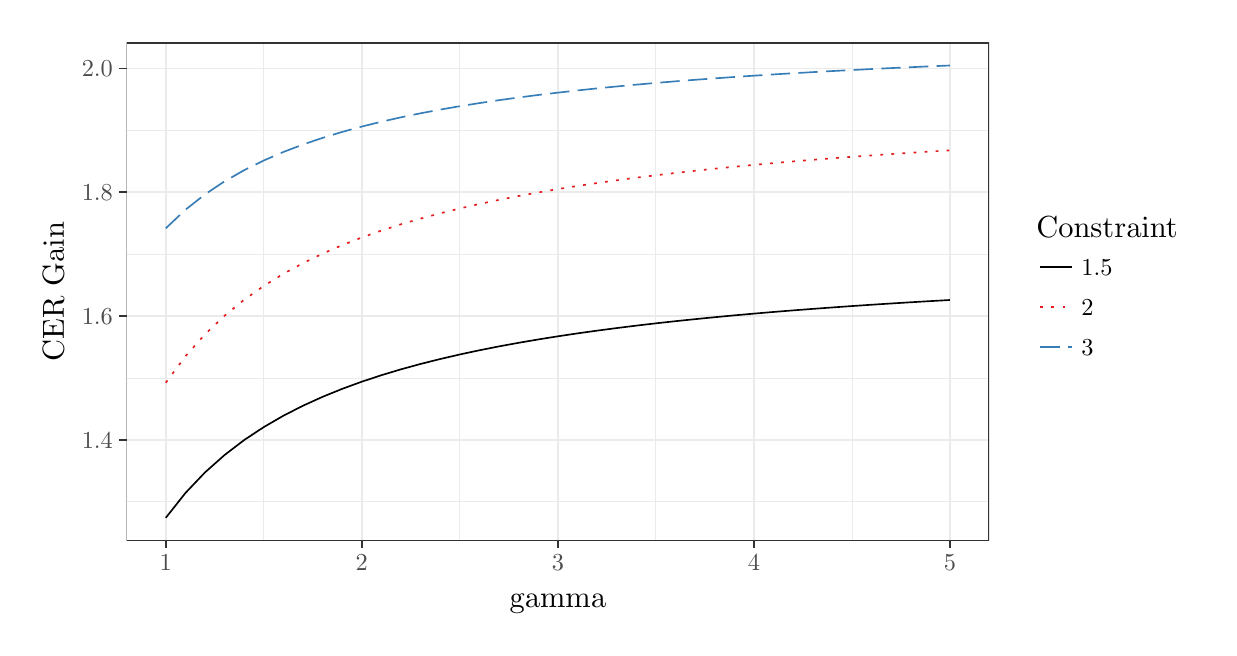
\begin{tikzpicture}[x=1pt,y=1pt]
\definecolor{fillColor}{RGB}{255,255,255}
\path[use as bounding box,fill=fillColor,fill opacity=0.00] (0,0) rectangle (426.79,216.81);
\begin{scope}
\path[clip] (  0.00,  0.00) rectangle (426.79,216.81);
\definecolor{drawColor}{RGB}{255,255,255}
\definecolor{fillColor}{RGB}{255,255,255}

\path[draw=drawColor,line width= 0.6pt,line join=round,line cap=round,fill=fillColor] (  0.00,  0.00) rectangle (426.79,216.81);
\end{scope}
\begin{scope}
\path[clip] ( 35.74, 31.53) rectangle (347.42,211.31);
\definecolor{fillColor}{RGB}{255,255,255}

\path[fill=fillColor] ( 35.74, 31.53) rectangle (347.42,211.31);
\definecolor{drawColor}{gray}{0.92}

\path[draw=drawColor,line width= 0.3pt,line join=round] ( 35.74, 45.51) --
	(347.42, 45.51);

\path[draw=drawColor,line width= 0.3pt,line join=round] ( 35.74, 90.23) --
	(347.42, 90.23);

\path[draw=drawColor,line width= 0.3pt,line join=round] ( 35.74,134.95) --
	(347.42,134.95);

\path[draw=drawColor,line width= 0.3pt,line join=round] ( 35.74,179.67) --
	(347.42,179.67);

\path[draw=drawColor,line width= 0.3pt,line join=round] ( 85.33, 31.53) --
	( 85.33,211.31);

\path[draw=drawColor,line width= 0.3pt,line join=round] (156.16, 31.53) --
	(156.16,211.31);

\path[draw=drawColor,line width= 0.3pt,line join=round] (227.00, 31.53) --
	(227.00,211.31);

\path[draw=drawColor,line width= 0.3pt,line join=round] (297.84, 31.53) --
	(297.84,211.31);

\path[draw=drawColor,line width= 0.6pt,line join=round] ( 35.74, 67.87) --
	(347.42, 67.87);

\path[draw=drawColor,line width= 0.6pt,line join=round] ( 35.74,112.59) --
	(347.42,112.59);

\path[draw=drawColor,line width= 0.6pt,line join=round] ( 35.74,157.31) --
	(347.42,157.31);

\path[draw=drawColor,line width= 0.6pt,line join=round] ( 35.74,202.03) --
	(347.42,202.03);

\path[draw=drawColor,line width= 0.6pt,line join=round] ( 49.91, 31.53) --
	( 49.91,211.31);

\path[draw=drawColor,line width= 0.6pt,line join=round] (120.74, 31.53) --
	(120.74,211.31);

\path[draw=drawColor,line width= 0.6pt,line join=round] (191.58, 31.53) --
	(191.58,211.31);

\path[draw=drawColor,line width= 0.6pt,line join=round] (262.42, 31.53) --
	(262.42,211.31);

\path[draw=drawColor,line width= 0.6pt,line join=round] (333.25, 31.53) --
	(333.25,211.31);
\definecolor{drawColor}{RGB}{0,0,0}

\path[draw=drawColor,line width= 0.6pt,line join=round] ( 49.91, 39.70) --
	( 56.99, 48.65) --
	( 64.07, 56.10) --
	( 71.16, 62.40) --
	( 78.24, 67.81) --
	( 85.33, 72.49) --
	( 92.41, 76.59) --
	( 99.49, 80.21) --
	(106.58, 83.42) --
	(113.66, 86.30) --
	(120.74, 88.89) --
	(127.83, 91.23) --
	(134.91, 93.36) --
	(141.99, 95.30) --
	(149.08, 97.08) --
	(156.16, 98.72) --
	(163.25,100.24) --
	(170.33,101.64) --
	(177.41,102.94) --
	(184.50,104.15) --
	(191.58,105.28) --
	(198.66,106.34) --
	(205.75,107.33) --
	(212.83,108.26) --
	(219.92,109.14) --
	(227.00,109.97) --
	(234.08,110.75) --
	(241.17,111.48) --
	(248.25,112.18) --
	(255.33,112.85) --
	(262.42,113.48) --
	(269.50,114.08) --
	(276.58,114.65) --
	(283.67,115.19) --
	(290.75,115.71) --
	(297.84,116.21) --
	(304.92,116.69) --
	(312.00,117.14) --
	(319.09,117.58) --
	(326.17,118.00) --
	(333.25,118.40);
\definecolor{drawColor}{RGB}{228,26,28}

\path[draw=drawColor,line width= 0.6pt,dash pattern=on 1pt off 3pt ,line join=round] ( 49.91, 88.51) --
	( 56.99, 98.05) --
	( 64.07,106.00) --
	( 71.16,112.73) --
	( 78.24,118.50) --
	( 85.33,123.49) --
	( 92.41,127.87) --
	( 99.49,131.73) --
	(106.58,135.16) --
	(113.66,138.23) --
	(120.74,140.99) --
	(127.83,143.49) --
	(134.91,145.76) --
	(141.99,147.83) --
	(149.08,149.73) --
	(156.16,151.48) --
	(163.25,153.10) --
	(170.33,154.59) --
	(177.41,155.98) --
	(184.50,157.27) --
	(191.58,158.48) --
	(198.66,159.61) --
	(205.75,160.67) --
	(212.83,161.66) --
	(219.92,162.60) --
	(227.00,163.48) --
	(234.08,164.31) --
	(241.17,165.10) --
	(248.25,165.85) --
	(255.33,166.55) --
	(262.42,167.23) --
	(269.50,167.87) --
	(276.58,168.48) --
	(283.67,169.06) --
	(290.75,169.61) --
	(297.84,170.14) --
	(304.92,170.65) --
	(312.00,171.14) --
	(319.09,171.60) --
	(326.17,172.05) --
	(333.25,172.48);
\definecolor{drawColor}{RGB}{55,126,184}

\path[draw=drawColor,line width= 0.6pt,dash pattern=on 7pt off 3pt ,line join=round] ( 49.91,144.31) --
	( 56.99,151.00) --
	( 64.07,156.57) --
	( 71.16,161.28) --
	( 78.24,165.32) --
	( 85.33,168.82) --
	( 92.41,171.89) --
	( 99.49,174.59) --
	(106.58,176.99) --
	(113.66,179.14) --
	(120.74,181.08) --
	(127.83,182.83) --
	(134.91,184.42) --
	(141.99,185.87) --
	(149.08,187.21) --
	(156.16,188.43) --
	(163.25,189.56) --
	(170.33,190.61) --
	(177.41,191.58) --
	(184.50,192.49) --
	(191.58,193.33) --
	(198.66,194.12) --
	(205.75,194.87) --
	(212.83,195.56) --
	(219.92,196.22) --
	(227.00,196.84) --
	(234.08,197.42) --
	(241.17,197.97) --
	(248.25,198.49) --
	(255.33,198.99) --
	(262.42,199.46) --
	(269.50,199.91) --
	(276.58,200.34) --
	(283.67,200.74) --
	(290.75,201.13) --
	(297.84,201.50) --
	(304.92,201.86) --
	(312.00,202.20) --
	(319.09,202.53) --
	(326.17,202.84) --
	(333.25,203.14);
\definecolor{drawColor}{gray}{0.20}

\path[draw=drawColor,line width= 0.6pt,line join=round,line cap=round] ( 35.74, 31.53) rectangle (347.42,211.31);
\end{scope}
\begin{scope}
\path[clip] (  0.00,  0.00) rectangle (426.79,216.81);
\definecolor{drawColor}{gray}{0.30}

\node[text=drawColor,anchor=base east,inner sep=0pt, outer sep=0pt, scale=  0.88] at ( 30.79, 64.84) {1.4};

\node[text=drawColor,anchor=base east,inner sep=0pt, outer sep=0pt, scale=  0.88] at ( 30.79,109.56) {1.6};

\node[text=drawColor,anchor=base east,inner sep=0pt, outer sep=0pt, scale=  0.88] at ( 30.79,154.28) {1.8};

\node[text=drawColor,anchor=base east,inner sep=0pt, outer sep=0pt, scale=  0.88] at ( 30.79,199.00) {2.0};
\end{scope}
\begin{scope}
\path[clip] (  0.00,  0.00) rectangle (426.79,216.81);
\definecolor{drawColor}{gray}{0.20}

\path[draw=drawColor,line width= 0.6pt,line join=round] ( 32.99, 67.87) --
	( 35.74, 67.87);

\path[draw=drawColor,line width= 0.6pt,line join=round] ( 32.99,112.59) --
	( 35.74,112.59);

\path[draw=drawColor,line width= 0.6pt,line join=round] ( 32.99,157.31) --
	( 35.74,157.31);

\path[draw=drawColor,line width= 0.6pt,line join=round] ( 32.99,202.03) --
	( 35.74,202.03);
\end{scope}
\begin{scope}
\path[clip] (  0.00,  0.00) rectangle (426.79,216.81);
\definecolor{drawColor}{gray}{0.20}

\path[draw=drawColor,line width= 0.6pt,line join=round] ( 49.91, 28.78) --
	( 49.91, 31.53);

\path[draw=drawColor,line width= 0.6pt,line join=round] (120.74, 28.78) --
	(120.74, 31.53);

\path[draw=drawColor,line width= 0.6pt,line join=round] (191.58, 28.78) --
	(191.58, 31.53);

\path[draw=drawColor,line width= 0.6pt,line join=round] (262.42, 28.78) --
	(262.42, 31.53);

\path[draw=drawColor,line width= 0.6pt,line join=round] (333.25, 28.78) --
	(333.25, 31.53);
\end{scope}
\begin{scope}
\path[clip] (  0.00,  0.00) rectangle (426.79,216.81);
\definecolor{drawColor}{gray}{0.30}

\node[text=drawColor,anchor=base,inner sep=0pt, outer sep=0pt, scale=  0.88] at ( 49.91, 20.52) {1};

\node[text=drawColor,anchor=base,inner sep=0pt, outer sep=0pt, scale=  0.88] at (120.74, 20.52) {2};

\node[text=drawColor,anchor=base,inner sep=0pt, outer sep=0pt, scale=  0.88] at (191.58, 20.52) {3};

\node[text=drawColor,anchor=base,inner sep=0pt, outer sep=0pt, scale=  0.88] at (262.42, 20.52) {4};

\node[text=drawColor,anchor=base,inner sep=0pt, outer sep=0pt, scale=  0.88] at (333.25, 20.52) {5};
\end{scope}
\begin{scope}
\path[clip] (  0.00,  0.00) rectangle (426.79,216.81);
\definecolor{drawColor}{RGB}{0,0,0}

\node[text=drawColor,anchor=base,inner sep=0pt, outer sep=0pt, scale=  1.10] at (191.58,  7.44) {gamma};
\end{scope}
\begin{scope}
\path[clip] (  0.00,  0.00) rectangle (426.79,216.81);
\definecolor{drawColor}{RGB}{0,0,0}

\node[text=drawColor,rotate= 90.00,anchor=base,inner sep=0pt, outer sep=0pt, scale=  1.10] at ( 13.08,121.42) {CER Gain};
\end{scope}
\begin{scope}
\path[clip] (  0.00,  0.00) rectangle (426.79,216.81);
\definecolor{fillColor}{RGB}{255,255,255}

\path[fill=fillColor] (358.80, 88.45) rectangle (421.29,154.39);
\end{scope}
\begin{scope}
\path[clip] (  0.00,  0.00) rectangle (426.79,216.81);
\definecolor{drawColor}{RGB}{0,0,0}

\node[text=drawColor,anchor=base west,inner sep=0pt, outer sep=0pt, scale=  1.10] at (364.49,141.12) {Constraint};
\end{scope}
\begin{scope}
\path[clip] (  0.00,  0.00) rectangle (426.79,216.81);
\definecolor{fillColor}{RGB}{255,255,255}

\path[fill=fillColor] (364.49,123.05) rectangle (378.95,137.51);
\end{scope}
\begin{scope}
\path[clip] (  0.00,  0.00) rectangle (426.79,216.81);
\definecolor{drawColor}{RGB}{0,0,0}

\path[draw=drawColor,line width= 0.6pt,line join=round] (365.94,130.28) -- (377.50,130.28);
\end{scope}
\begin{scope}
\path[clip] (  0.00,  0.00) rectangle (426.79,216.81);
\definecolor{fillColor}{RGB}{255,255,255}

\path[fill=fillColor] (364.49,108.60) rectangle (378.95,123.05);
\end{scope}
\begin{scope}
\path[clip] (  0.00,  0.00) rectangle (426.79,216.81);
\definecolor{drawColor}{RGB}{228,26,28}

\path[draw=drawColor,line width= 0.6pt,dash pattern=on 1pt off 3pt ,line join=round] (365.94,115.83) -- (377.50,115.83);
\end{scope}
\begin{scope}
\path[clip] (  0.00,  0.00) rectangle (426.79,216.81);
\definecolor{fillColor}{RGB}{255,255,255}

\path[fill=fillColor] (364.49, 94.14) rectangle (378.95,108.60);
\end{scope}
\begin{scope}
\path[clip] (  0.00,  0.00) rectangle (426.79,216.81);
\definecolor{drawColor}{RGB}{55,126,184}

\path[draw=drawColor,line width= 0.6pt,dash pattern=on 7pt off 3pt ,line join=round] (365.94,101.37) -- (377.50,101.37);
\end{scope}
\begin{scope}
\path[clip] (  0.00,  0.00) rectangle (426.79,216.81);
\definecolor{drawColor}{RGB}{0,0,0}

\node[text=drawColor,anchor=base west,inner sep=0pt, outer sep=0pt, scale=  0.88] at (380.75,127.25) {1.5};
\end{scope}
\begin{scope}
\path[clip] (  0.00,  0.00) rectangle (426.79,216.81);
\definecolor{drawColor}{RGB}{0,0,0}

\node[text=drawColor,anchor=base west,inner sep=0pt, outer sep=0pt, scale=  0.88] at (380.75,112.80) {2};
\end{scope}
\begin{scope}
\path[clip] (  0.00,  0.00) rectangle (426.79,216.81);
\definecolor{drawColor}{RGB}{0,0,0}

\node[text=drawColor,anchor=base west,inner sep=0pt, outer sep=0pt, scale=  0.88] at (380.75, 98.34) {3};
\end{scope}
\end{tikzpicture}
}
	\end{figure}
	}
	\only<2-3>{
		\begin{figure}
			\resizebox{11cm}{6cm}{% Created by tikzDevice version 0.10.1 on 2018-06-14 11:50:00
% !TEX encoding = UTF-8 Unicode
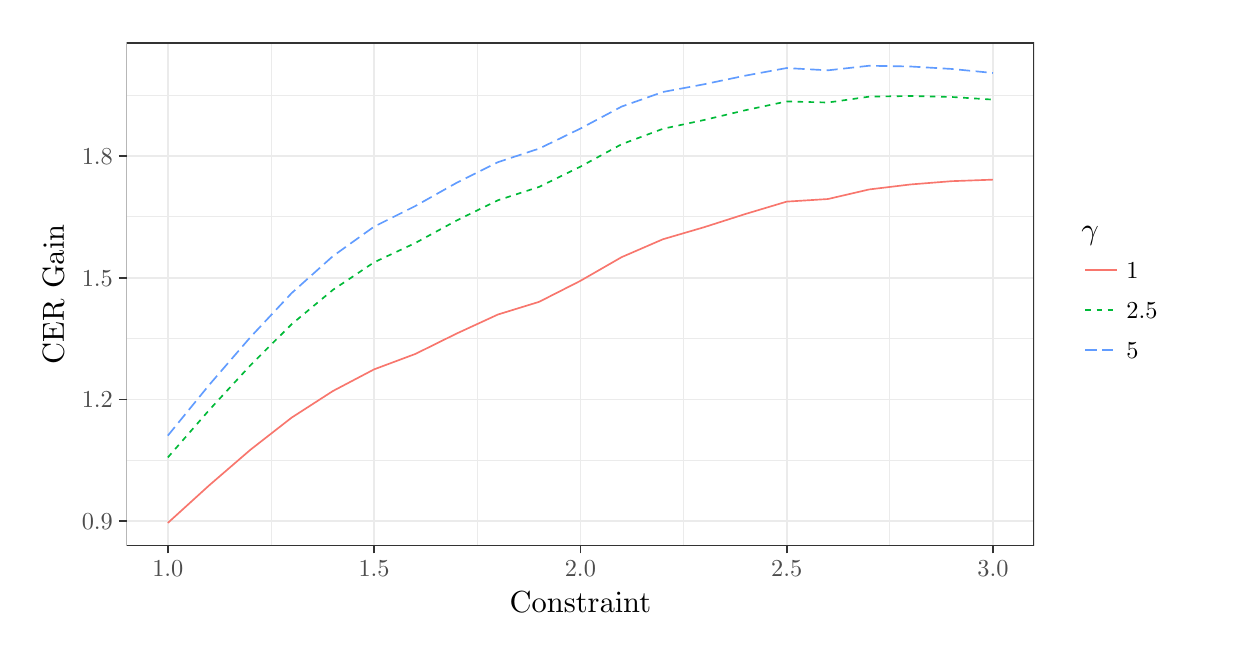
\begin{tikzpicture}[x=1pt,y=1pt]
\definecolor{fillColor}{RGB}{255,255,255}
\path[use as bounding box,fill=fillColor,fill opacity=0.00] (0,0) rectangle (426.79,216.81);
\begin{scope}
\path[clip] (  0.00,  0.00) rectangle (426.79,216.81);
\definecolor{drawColor}{RGB}{255,255,255}
\definecolor{fillColor}{RGB}{255,255,255}

\path[draw=drawColor,line width= 0.6pt,line join=round,line cap=round,fill=fillColor] (  0.00,  0.00) rectangle (426.79,216.81);
\end{scope}
\begin{scope}
\path[clip] ( 35.74, 29.59) rectangle (363.70,211.31);
\definecolor{fillColor}{RGB}{255,255,255}

\path[fill=fillColor] ( 35.74, 29.59) rectangle (363.70,211.31);
\definecolor{drawColor}{gray}{0.92}

\path[draw=drawColor,line width= 0.3pt,line join=round] ( 35.74, 60.51) --
	(363.70, 60.51);

\path[draw=drawColor,line width= 0.3pt,line join=round] ( 35.74,104.47) --
	(363.70,104.47);

\path[draw=drawColor,line width= 0.3pt,line join=round] ( 35.74,148.43) --
	(363.70,148.43);

\path[draw=drawColor,line width= 0.3pt,line join=round] ( 35.74,192.39) --
	(363.70,192.39);

\path[draw=drawColor,line width= 0.3pt,line join=round] ( 87.92, 29.59) --
	( 87.92,211.31);

\path[draw=drawColor,line width= 0.3pt,line join=round] (162.45, 29.59) --
	(162.45,211.31);

\path[draw=drawColor,line width= 0.3pt,line join=round] (236.99, 29.59) --
	(236.99,211.31);

\path[draw=drawColor,line width= 0.3pt,line join=round] (311.53, 29.59) --
	(311.53,211.31);

\path[draw=drawColor,line width= 0.6pt,line join=round] ( 35.74, 38.53) --
	(363.70, 38.53);

\path[draw=drawColor,line width= 0.6pt,line join=round] ( 35.74, 82.49) --
	(363.70, 82.49);

\path[draw=drawColor,line width= 0.6pt,line join=round] ( 35.74,126.45) --
	(363.70,126.45);

\path[draw=drawColor,line width= 0.6pt,line join=round] ( 35.74,170.41) --
	(363.70,170.41);

\path[draw=drawColor,line width= 0.6pt,line join=round] ( 50.65, 29.59) --
	( 50.65,211.31);

\path[draw=drawColor,line width= 0.6pt,line join=round] (125.18, 29.59) --
	(125.18,211.31);

\path[draw=drawColor,line width= 0.6pt,line join=round] (199.72, 29.59) --
	(199.72,211.31);

\path[draw=drawColor,line width= 0.6pt,line join=round] (274.26, 29.59) --
	(274.26,211.31);

\path[draw=drawColor,line width= 0.6pt,line join=round] (348.80, 29.59) --
	(348.80,211.31);
\definecolor{drawColor}{RGB}{248,118,109}

\path[draw=drawColor,line width= 0.6pt,line join=round] ( 50.65, 37.85) --
	( 65.55, 51.39) --
	( 80.46, 64.26) --
	( 95.37, 75.89) --
	(110.28, 85.50) --
	(125.18, 93.34) --
	(140.09, 98.91) --
	(155.00,106.28) --
	(169.91,113.15) --
	(184.81,117.74) --
	(199.72,125.32) --
	(214.63,133.89) --
	(229.54,140.35) --
	(244.44,144.71) --
	(259.35,149.48) --
	(274.26,153.95) --
	(289.17,154.89) --
	(304.07,158.35) --
	(318.98,160.15) --
	(333.89,161.34) --
	(348.80,161.89);
\definecolor{drawColor}{RGB}{0,186,56}

\path[draw=drawColor,line width= 0.6pt,dash pattern=on 2pt off 2pt ,line join=round] ( 50.65, 61.51) --
	( 65.55, 78.60) --
	( 80.46, 94.77) --
	( 95.37,109.64) --
	(110.28,122.05) --
	(125.18,132.02) --
	(140.09,139.01) --
	(155.00,147.13) --
	(169.91,154.44) --
	(184.81,159.27) --
	(199.72,166.59) --
	(214.63,174.70) --
	(229.54,180.27) --
	(244.44,183.45) --
	(259.35,186.98) --
	(274.26,190.15) --
	(289.17,189.76) --
	(304.07,191.88) --
	(318.98,192.12) --
	(333.89,191.76) --
	(348.80,190.81);
\definecolor{drawColor}{RGB}{97,156,255}

\path[draw=drawColor,line width= 0.6pt,dash pattern=on 4pt off 2pt ,line join=round] ( 50.65, 69.40) --
	( 65.55, 87.67) --
	( 80.46,104.94) --
	( 95.37,120.88) --
	(110.28,134.24) --
	(125.18,144.91) --
	(140.09,152.37) --
	(155.00,160.75) --
	(169.91,168.21) --
	(184.81,173.11) --
	(199.72,180.35) --
	(214.63,188.30) --
	(229.54,193.57) --
	(244.44,196.36) --
	(259.35,199.48) --
	(274.26,202.22) --
	(289.17,201.39) --
	(304.07,203.05) --
	(318.98,202.78) --
	(333.89,201.89) --
	(348.80,200.44);
\definecolor{drawColor}{gray}{0.20}

\path[draw=drawColor,line width= 0.6pt,line join=round,line cap=round] ( 35.74, 29.59) rectangle (363.70,211.31);
\end{scope}
\begin{scope}
\path[clip] (  0.00,  0.00) rectangle (426.79,216.81);
\definecolor{drawColor}{gray}{0.30}

\node[text=drawColor,anchor=base east,inner sep=0pt, outer sep=0pt, scale=  0.88] at ( 30.79, 35.50) {0.9};

\node[text=drawColor,anchor=base east,inner sep=0pt, outer sep=0pt, scale=  0.88] at ( 30.79, 79.46) {1.2};

\node[text=drawColor,anchor=base east,inner sep=0pt, outer sep=0pt, scale=  0.88] at ( 30.79,123.42) {1.5};

\node[text=drawColor,anchor=base east,inner sep=0pt, outer sep=0pt, scale=  0.88] at ( 30.79,167.38) {1.8};
\end{scope}
\begin{scope}
\path[clip] (  0.00,  0.00) rectangle (426.79,216.81);
\definecolor{drawColor}{gray}{0.20}

\path[draw=drawColor,line width= 0.6pt,line join=round] ( 32.99, 38.53) --
	( 35.74, 38.53);

\path[draw=drawColor,line width= 0.6pt,line join=round] ( 32.99, 82.49) --
	( 35.74, 82.49);

\path[draw=drawColor,line width= 0.6pt,line join=round] ( 32.99,126.45) --
	( 35.74,126.45);

\path[draw=drawColor,line width= 0.6pt,line join=round] ( 32.99,170.41) --
	( 35.74,170.41);
\end{scope}
\begin{scope}
\path[clip] (  0.00,  0.00) rectangle (426.79,216.81);
\definecolor{drawColor}{gray}{0.20}

\path[draw=drawColor,line width= 0.6pt,line join=round] ( 50.65, 26.84) --
	( 50.65, 29.59);

\path[draw=drawColor,line width= 0.6pt,line join=round] (125.18, 26.84) --
	(125.18, 29.59);

\path[draw=drawColor,line width= 0.6pt,line join=round] (199.72, 26.84) --
	(199.72, 29.59);

\path[draw=drawColor,line width= 0.6pt,line join=round] (274.26, 26.84) --
	(274.26, 29.59);

\path[draw=drawColor,line width= 0.6pt,line join=round] (348.80, 26.84) --
	(348.80, 29.59);
\end{scope}
\begin{scope}
\path[clip] (  0.00,  0.00) rectangle (426.79,216.81);
\definecolor{drawColor}{gray}{0.30}

\node[text=drawColor,anchor=base,inner sep=0pt, outer sep=0pt, scale=  0.88] at ( 50.65, 18.58) {1.0};

\node[text=drawColor,anchor=base,inner sep=0pt, outer sep=0pt, scale=  0.88] at (125.18, 18.58) {1.5};

\node[text=drawColor,anchor=base,inner sep=0pt, outer sep=0pt, scale=  0.88] at (199.72, 18.58) {2.0};

\node[text=drawColor,anchor=base,inner sep=0pt, outer sep=0pt, scale=  0.88] at (274.26, 18.58) {2.5};

\node[text=drawColor,anchor=base,inner sep=0pt, outer sep=0pt, scale=  0.88] at (348.80, 18.58) {3.0};
\end{scope}
\begin{scope}
\path[clip] (  0.00,  0.00) rectangle (426.79,216.81);
\definecolor{drawColor}{RGB}{0,0,0}

\node[text=drawColor,anchor=base,inner sep=0pt, outer sep=0pt, scale=  1.10] at (199.72,  5.50) {Constraint};
\end{scope}
\begin{scope}
\path[clip] (  0.00,  0.00) rectangle (426.79,216.81);
\definecolor{drawColor}{RGB}{0,0,0}

\node[text=drawColor,rotate= 90.00,anchor=base,inner sep=0pt, outer sep=0pt, scale=  1.10] at ( 13.08,120.45) {CER Gain};
\end{scope}
\begin{scope}
\path[clip] (  0.00,  0.00) rectangle (426.79,216.81);
\definecolor{fillColor}{RGB}{255,255,255}

\path[fill=fillColor] (375.09, 87.48) rectangle (421.29,153.41);
\end{scope}
\begin{scope}
\path[clip] (  0.00,  0.00) rectangle (426.79,216.81);
\definecolor{drawColor}{RGB}{0,0,0}

\node[text=drawColor,anchor=base west,inner sep=0pt, outer sep=0pt, scale=  1.10] at (380.78,140.15) {$\gamma$};
\end{scope}
\begin{scope}
\path[clip] (  0.00,  0.00) rectangle (426.79,216.81);
\definecolor{fillColor}{RGB}{255,255,255}

\path[fill=fillColor] (380.78,122.08) rectangle (395.23,136.53);
\end{scope}
\begin{scope}
\path[clip] (  0.00,  0.00) rectangle (426.79,216.81);
\definecolor{drawColor}{RGB}{248,118,109}

\path[draw=drawColor,line width= 0.6pt,line join=round] (382.22,129.31) -- (393.78,129.31);
\end{scope}
\begin{scope}
\path[clip] (  0.00,  0.00) rectangle (426.79,216.81);
\definecolor{fillColor}{RGB}{255,255,255}

\path[fill=fillColor] (380.78,107.63) rectangle (395.23,122.08);
\end{scope}
\begin{scope}
\path[clip] (  0.00,  0.00) rectangle (426.79,216.81);
\definecolor{drawColor}{RGB}{0,186,56}

\path[draw=drawColor,line width= 0.6pt,dash pattern=on 2pt off 2pt ,line join=round] (382.22,114.85) -- (393.78,114.85);
\end{scope}
\begin{scope}
\path[clip] (  0.00,  0.00) rectangle (426.79,216.81);
\definecolor{fillColor}{RGB}{255,255,255}

\path[fill=fillColor] (380.78, 93.17) rectangle (395.23,107.63);
\end{scope}
\begin{scope}
\path[clip] (  0.00,  0.00) rectangle (426.79,216.81);
\definecolor{drawColor}{RGB}{97,156,255}

\path[draw=drawColor,line width= 0.6pt,dash pattern=on 4pt off 2pt ,line join=round] (382.22,100.40) -- (393.78,100.40);
\end{scope}
\begin{scope}
\path[clip] (  0.00,  0.00) rectangle (426.79,216.81);
\definecolor{drawColor}{RGB}{0,0,0}

\node[text=drawColor,anchor=base west,inner sep=0pt, outer sep=0pt, scale=  0.88] at (397.04,126.28) {1};
\end{scope}
\begin{scope}
\path[clip] (  0.00,  0.00) rectangle (426.79,216.81);
\definecolor{drawColor}{RGB}{0,0,0}

\node[text=drawColor,anchor=base west,inner sep=0pt, outer sep=0pt, scale=  0.88] at (397.04,111.82) {2.5};
\end{scope}
\begin{scope}
\path[clip] (  0.00,  0.00) rectangle (426.79,216.81);
\definecolor{drawColor}{RGB}{0,0,0}

\node[text=drawColor,anchor=base west,inner sep=0pt, outer sep=0pt, scale=  0.88] at (397.04, 97.37) {5};
\end{scope}
\end{tikzpicture}
}
		\end{figure}
	}
	\only<3>{\begin{itemize}
			\item Stochastic dominance tests show that non-EUT investors prefer AV management.
		\end{itemize}}
\end{frame}

\subsection{Systematic Risk}

\begin{frame}{Suggestively Systematic}
	\begin{itemize}[<+->]
		\item CRSP dialy returns contain only NYSE firms, are shallower, more illiquid, and investment was not a meaningful part of aggregate wealth 1926 - 1962 - NYSE (2016) and Taylor (2014) 
		\item AC should not predict returns 1926 - 1962
		\item AV management should work globally
		\item AV management using the AV of equity returns should generate better performance across asset classes
		\item AV managed returns should depend systematically on the representativeness of daily returns
	\end{itemize}
\end{frame}

\begin{frame}{Regression Sub-samples}
	\begin{adjustbox}{width=\textwidth}
		
% Table created by stargazer v.5.2 by Marek Hlavac, Harvard University. E-mail: hlavac at fas.harvard.edu
% Date and time: Fri, Jun 08, 2018 - 12:59:10  IST
\begin{tabular}{@{\extracolsep{5pt}}lccccc} 
\\[-1.8ex]\hline 
\hline \\[-1.8ex] 
\\[-1.8ex] & \multicolumn{5}{c}{RET$_{t+1}$} \\ 
\hline \\[-1.8ex] 
 AV & 0.063 &  &  & 0.117$^{**}$ & 0.296$^{***}$ \\ 
  & p = 0.189 &  &  & p = 0.046 & p = 0.002 \\ 
  & & & & & \\ 
 AC &  & $-$0.027 &  & $-$0.094 &  \\ 
  &  & p = 0.580 &  & p = 0.110 &  \\ 
  & & & & & \\ 
 SV &  &  & $-$0.024 &  & $-$0.275$^{***}$ \\ 
  &  &  & p = 0.613 &  & p = 0.003 \\ 
  & & & & & \\ 
 Constant & $-$0.0001 & 0.0001 & 0.00003 & 0.0001 & 0.00004 \\ 
  & p = 1.000 & p = 1.000 & p = 1.000 & p = 0.999 & p = 1.000 \\ 
  & & & & & \\ 
\textit{N} & 431 & 431 & 431 & 431 & 431 \\ 
R$^{2}$ & 0.004 & 0.001 & 0.001 & 0.010 & 0.026 \\ 
Adjusted R$^{2}$ & 0.002 & $-$0.002 & $-$0.002 & 0.005 & 0.021 \\ 
\hline 
\hline \\[-1.8ex] 
\textit{Notes:} & \multicolumn{5}{r}{$^{***}$Significant at the 1 percent level.} \\ 
 & \multicolumn{5}{r}{$^{**}$Significant at the 5 percent level.} \\ 
 & \multicolumn{5}{r}{$^{*}$Significant at the 10 percent level.} \\ 
\end{tabular} 

	\end{adjustbox}
	\begin{adjustbox}{width=\textwidth}
		
% Table created by stargazer v.5.2 by Marek Hlavac, Harvard University. E-mail: hlavac at fas.harvard.edu
% Date and time: Fri, Jun 08, 2018 - 01:03:43  IST
\begin{tabular}{@{\extracolsep{5pt}}lccccc} 
\\[-1.8ex]\hline 
\hline \\[-1.8ex] 
\\[-1.8ex] & \multicolumn{5}{c}{RET$_{t+1}$} \\ 
\hline \\[-1.8ex] 
 AV & $-$0.130$^{***}$ &  &  & $-$0.168$^{***}$ & $-$0.173$^{*}$ \\ 
  & p = 0.001 &  &  & p = 0.0001 & p = 0.052 \\ 
  & & & & & \\ 
 AC &  & 0.049 &  & 0.108$^{***}$ &  \\ 
  &  & p = 0.212 &  & p = 0.010 &  \\ 
  & & & & & \\ 
 SV &  &  & $-$0.107$^{***}$ &  & 0.048 \\ 
  &  &  & p = 0.006 &  & p = 0.588 \\ 
  & & & & & \\ 
 Constant & $-$0.000 & $-$0.000 & $-$0.000 & $-$0.000 & $-$0.000 \\ 
  & p = 1.000 & p = 1.000 & p = 1.000 & p = 1.000 & p = 1.000 \\ 
  & & & & & \\ 
\textit{N} & 655 & 655 & 655 & 655 & 655 \\ 
R$^{2}$ & 0.017 & 0.002 & 0.012 & 0.027 & 0.017 \\ 
Adjusted R$^{2}$ & 0.015 & 0.001 & 0.010 & 0.024 & 0.014 \\ 
\hline 
\hline \\[-1.8ex] 
\textit{Notes:} & \multicolumn{5}{r}{$^{***}$Significant at the 1 percent level.} \\ 
 & \multicolumn{5}{r}{$^{**}$Significant at the 5 percent level.} \\ 
 & \multicolumn{5}{r}{$^{*}$Significant at the 10 percent level.} \\ 
\end{tabular} 

	\end{adjustbox}
\end{frame}

\begin{frame}{Global Performance}
	\begin{adjustbox}{width=\textwidth}
		\begin{tabular}{@{\extracolsep{5pt}} ccccccc} 
			\\[-1.8ex]\hline 
			\hline \\[-1.8ex]
			& \multicolumn{2}{c}{AV} &\multicolumn{2}{c}{SV}& \multicolumn{2}{c}{BH}\\
			\cline{2-3} \cline{4-5} \cline{6-7}\\
			Country & RET & Sharpe & RET & Sharpe & RET & Sharpe \\ 
			\hline \\[-1.8ex] 
			AUS & 12.477*** & 0.981 & 11.993 & 0.943 & 7.805 & 0.614 \\ 
			BRA & 11.000*** & 0.291 & 9.037 & 0.240 & 6.163 & 0.164 \\ 
			CHN & 27.381 & 0.868 & 24.926 & 0.790 & 12.286 & 0.390 \\ 
			DEU & 11.064*** & 0.537* & 7.633 & 0.371 & 5.399 & 0.262 \\ 
			FRA & 7.243*** & 0.404 & 6.128 & 0.341 & 4.904 & 0.273 \\ 
			IND & 14.893*** & 0.633 & 12.256 & 0.521 & 11.460 & 0.487 \\ 
			ITA & 3.838 & 0.194 & 3.912 & 0.198 & 1.451 & 0.073 \\ 
			JPN & 1.375*** & 0.068 & 0.129 & 0.006 & -0.775 & -0.038 \\ 
			UK & 6.591*** & 0.485 & 5.984 & 0.441 & 5.111 & 0.376 \\ 
			%USA & 9.739*** & 0.517* & 8.57 & 0.455 & 5.994 & 0.318 \\
			World & 8.603$^{***}$ & 0.551 &  8.306 & 0.536  & 4.484 & 0.290\\
			\hline \\[-1.8ex] 
		\end{tabular} 
	\end{adjustbox}
\end{frame}

\begin{frame}{Systematic Performance}
	\begin{center}
	Global Long - Short\\
	Ratio of Market RET to Wealth$\dagger$ RET ($w_{s,t}$)
	\end{center}
	\vspace{-6pt}
	\begin{adjustbox}{width=\textwidth}
		\begin{tabular}{lccccc}
			\hline\\[-1.8ex]
%			\multicolumn{6}{c}{Market RET to Wealth RET}\\
%			\hline\\[-1.8ex]
			& RET & Sharpe & $\alpha_{FF3}$ & $\alpha_{FF5}$ & $\alpha_{FF5+Mom}$ \\
			\cline{2-6}
			Long & 12.601 & 0.747 & 9.484$^{**}$ & 7.909$^{*}$ & 7.725$^{*}$ \\
			Short & 7.537 & 0.562 & 5.038$^{*}$ & 5.422$^{*}$ & 5.318$^{*}$ \\
			Long - Short & 5.065 & 0.405 & 4.446$^{***}$ & 2.488$^{***}$ & 2.407$^{**}$ \\
			\hline\\[-1.8ex]
		\end{tabular}
	\end{adjustbox}
	$\dagger$ Credit Suisse annual reports on global wealth (2000-2017)
\end{frame}

\begin{frame}{Economy-Wide Performance}
	\begin{center}
		Investment weight in other asset classes managed by equity AV
	\end{center}
	\vspace{-6pt}
	\begin{adjustbox}{width=\textwidth}
\begin{tabular}{@{\extracolsep{5pt}} Hccccccc} 
	\\[-1.8ex]\hline 
	\hline \\[-1.8ex] 
	& & \multicolumn{2}{c}{AV} &\multicolumn{2}{c}{SV}& \multicolumn{2}{c}{BH}\\
	\cline{3-4} \cline{5-6} \cline{7-8}\\
	& Index & RET & Sharpe & RET & Sharpe & RET & Sharpe \\ 
	\hline \\[-1.8ex] 
	1 & Dollar$_{BB}$ & $1.324^{***}$ & $0.170$ & $0.606$ & $0.078$ & $-0.296$ & $-0.038$ \\ 
	
	3 & Curr$_{DB}$ & $1.195^{***}$ & $0.272^{*}$ & $-0.668$ & $-0.152$ & $-0.244$ & $-0.056$ \\ 
	4 & Carry$_{DB}$ & $1.440^{***}$ & $0.134$ & $-0.361$ & $-0.033$ & $-2.071$ & $-0.192$ \\ 
	%5 & dbmom & $1.540$ & $0.170$ & $-0.854$ & $-0.094$ & $-0.226$ & $-0.025$ \\ 
	6 & Mom$_{DB}$ & $1.942^{***}$ & $0.214$ & $0.413$ & $0.045$ & $1.095$ & $0.120$ \\ 
	%7 & dbval & $0.148$ & $0.020$ & $0.847$ & $0.112$ & $1.466$ & $0.194$ \\ 
	2 & REIT$_{S\&P}$ & $26.706^{***}$ & $0.995$ & $14.980$ & $0.558$ & $5.302$ & $0.198$ \\ 
	8 & Comm$_{BB}$ & $-5.579^{***}$ & $-0.303$ & $-6.431$ & $-0.349$ & $-5.279$ & $-0.286$ \\ 
	%9 & gscom & $-5.799$ & $-0.250$ & $-4.371$ & $-0.188$ & $-2.741$ & $-0.118$ \\ 
	10 & Bond$_{Univ}$ & 3.951*** & 1.168*** & 1.436 & 0.425 & 3.276 & 0.969 \\ 
	%11 & bbUSagg & 3.381*** & 0.969** & 1.341 & 0.384 & 3.357 & 0.962 \\ 
	\hline \\[-1.8ex] 
\end{tabular} 
	\end{adjustbox}
\end{frame}

%\begin{frame}{Contribution}
%	\onslide<+->{\begin{block}{Variance Management}
%			\begin{itemize}[<+->]
%				\item Moreira and Muir (2017) and Hocquard, Ng, and Papageorgiou (2013)
%				\item AV is a better dynamic volatility management signal - returns, ratios, drawdowns, costs
%				\item AV management works globally and across asset classes (SV does not)
%			\end{itemize}
%		\end{block}}
%		\onslide<+->{\begin{block}{Risk Dynamics}
%				\begin{itemize}[<+->]
%					\item Gonzlez-Urteaga and Rubio (2016) and Bollerslev, Hood, Huss, and Pedersen (2017)
%					\item AV comes from the foundations of investment risk
%					\item Responds to the mix of systematic and non-systematic risk
%					\item AV is related to global non-systematic risk across asset classes
%				\end{itemize}}
%			\end{block}		
%		\end{frame}


%\begin{frame}{Global Equity Performance}
%	\onslide<+->{\begin{block}{Global Equity}
%		\begin{itemize}[<+->]
%			\item AV better in 8 of 9 international markets
%			\item AV better for globally diversified equity portfolio
%		\end{itemize}
%	\end{block}}
%	\onslide<+->{\begin{block}{Other Asset Classes}
%		\begin{itemize}[<+->]
%			\item AV better across currency indices
%			\item AV better real estate investment management
%		\end{itemize}}
%	\end{block}
%	\onslide<+->{This is consistent with the notion that AV management times investment to systematic risk for which investors are compensated and minimizes non-systematic risk.}
%\end{frame}

\section{Conclusion}

\begin{frame}{Conclusion}
	\onslide<+->{\begin{block}{Variance Management}
			\begin{itemize}[<+->]
				\item Moreira and Muir (2017) and Hocquard, Ng, and Papageorgiou (2013)
				\item AV is a better dynamic volatility management signal - returns, ratios, drawdowns, costs
				\item AV management works globally and across asset classes (SV does not)
			\end{itemize}
		\end{block}}
		\onslide<+->{\begin{block}{Risk Dynamics}
				\begin{itemize}[<+->]
					\item Gonzlez-Urteaga and Rubio (2016) and Bollerslev, Hood, Huss, and Pedersen (2017)
					\item AV comes from the foundations of investment risk
					\item AV management informs about the risk mix across the economy
				\end{itemize}}
			\end{block}		
\end{frame}

%\section{Conclusion}
%\begin{frame}{Conclusion}
%	\begin{itemize}
%		\item AV management is better than SV: higher returns, better ratios, lower costs
%		\item As such, AV management is a useful signal both globally and across assets classes where SV management does not perform
%		\item AV management is better because it times moving in and out of investments to changes in systematic risk which is compensated and non-systematic risk which is not
%		\item AV management informs about the risk mix across the economy
%		\item Thank you
%	\end{itemize}
%\end{frame}

\section{Data}
\begin{frame}{Equity Data}
		\begin{adjustbox}{width=\textwidth}
	\begin{tabular}{ccccc}
		\multicolumn{5}{c}{Equity Data}\\
		\hline \hline \\[-1.8ex] 
		Country & Start & Obs & Index & Assets\\
		\hline\\[-1.8ex]
		USA & 1926 - 8 & 1085 & CRSP & 500\\
		AUS & 2000 - 5 & $212$& ASX & $200$ \\ 
		BRA & 1995 - 2 & $275$& iShares MSCI Brazil ETF& $60$ \\ 
		CHN & 2005 - 5 & $152$& CSI 300& $300$ \\ 
		DEU & 1993 - 11 & $290$& HDAX& $110$ \\
		FRA & 1993 - 9 & $292$& SBF 120& $120$ \\ 
		IND & 2000 - 5 & $212$& Nifty 50& $50$ \\ 
		ITA & 2003 - 8 & $173$& FTSE MIB& $40$ \\ 
		JPN & 1993 - 6 & $295$& Nikkei& $255$ \\ 
		UK & 1993 - 6 & $295$& FTSE& $100$ \\ 
		World & 1995 - 3 & 274 & MSCI ACWI & 1735\\
		\hline
	\end{tabular}
		\end{adjustbox}
\end{frame}

\begin{frame}{Non-Equity Data}
	\begin{adjustbox}{width=\textwidth}
		\begin{tabular}{ccccc}
			\multicolumn{4}{c}{Other Asset Data}\\
			\hline \hline \\[-1.8ex] 
			Index & Start & Obs & Asset Class\\
			\hline\\
			Bloomberg US Spot & 2005 - 6 & 158 & Currency\\
			Deutsche Bank Currency & 2005 - 6 & $158$& Currency \\ 
			Deutsche Bank Carry & 2005 - 6 & $158$& Currency \\ 
			Deutsche Bank Momentum & 2005 - 6 & $158$& Currency \\ 
			S\&P REIT Index & 2005 - 6 & $158$& Real Estate \\
			Bloomberg Commodity & 2005 - 6 &158 & Commodities\\
			\hline
		\end{tabular}
	\end{adjustbox}
\end{frame}
\begin{frame}{AV Construction}
		\begin{itemize}
			%\item for month t, with T trading days, R$_{s,T}$ is the daily CRSP market return
			\item SV$_{t}$ = $\sigma^{2}_{S,t}$
			\item With m assets in the market, AV$_{t}$ = $\sum_{m=1}^{M} w_{m,t}\sigma^{2}_{m,t}$
			\item $W_{t}$ = $\frac{c}{X}$ is the investment weight in the portfolio, where X $\in$ \{AV$_{t-1}$,SV$_{t-1}$\}
			\item The constant c$_{target}$ is used to control the volatility of the strategy
			\item c$_{BH}$ matching the buy and hold
			\item For robustness, c$_{10}$ and c$_{12}$ targeting 10\% or 12\% annual return volatility
		\end{itemize}
\end{frame}

\section{Results}
\subsection{Investment}
\begin{frame}{Investment Weights}
			\begin{figure}
			\scalebox{.52}{% Created by tikzDevice version 0.10.1 on 2018-04-25 22:45:19
% !TEX encoding = UTF-8 Unicode
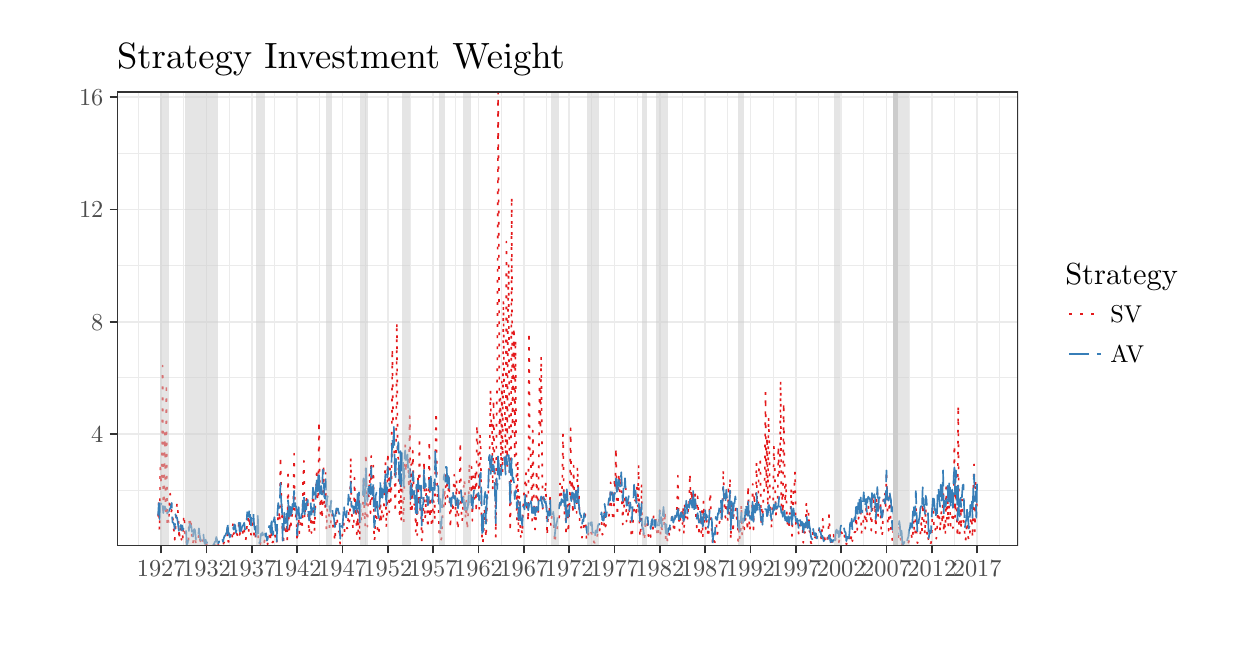
\begin{tikzpicture}[x=1pt,y=1pt]
\definecolor{fillColor}{RGB}{255,255,255}
\path[use as bounding box,fill=fillColor,fill opacity=0.00] (0,0) rectangle (426.79,216.81);
\begin{scope}
\path[clip] (  0.00,  0.00) rectangle (426.79,216.81);
\definecolor{drawColor}{RGB}{255,255,255}
\definecolor{fillColor}{RGB}{255,255,255}

\path[draw=drawColor,line width= 0.6pt,line join=round,line cap=round,fill=fillColor] (  0.00,  0.00) rectangle (426.79,216.81);
\end{scope}
\begin{scope}
\path[clip] ( 32.32, 29.59) rectangle (357.87,193.67);
\definecolor{fillColor}{RGB}{255,255,255}

\path[fill=fillColor] ( 32.32, 29.59) rectangle (357.87,193.67);
\definecolor{drawColor}{gray}{0.92}

\path[draw=drawColor,line width= 0.3pt,line join=round] ( 32.32, 49.71) --
	(357.87, 49.71);

\path[draw=drawColor,line width= 0.3pt,line join=round] ( 32.32, 90.28) --
	(357.87, 90.28);

\path[draw=drawColor,line width= 0.3pt,line join=round] ( 32.32,130.86) --
	(357.87,130.86);

\path[draw=drawColor,line width= 0.3pt,line join=round] ( 32.32,171.43) --
	(357.87,171.43);

\path[draw=drawColor,line width= 0.3pt,line join=round] ( 40.06, 29.59) --
	( 40.06,193.67);

\path[draw=drawColor,line width= 0.3pt,line join=round] ( 56.44, 29.59) --
	( 56.44,193.67);

\path[draw=drawColor,line width= 0.3pt,line join=round] ( 72.82, 29.59) --
	( 72.82,193.67);

\path[draw=drawColor,line width= 0.3pt,line join=round] ( 89.21, 29.59) --
	( 89.21,193.67);

\path[draw=drawColor,line width= 0.3pt,line join=round] (105.58, 29.59) --
	(105.58,193.67);

\path[draw=drawColor,line width= 0.3pt,line join=round] (121.96, 29.59) --
	(121.96,193.67);

\path[draw=drawColor,line width= 0.3pt,line join=round] (138.35, 29.59) --
	(138.35,193.67);

\path[draw=drawColor,line width= 0.3pt,line join=round] (154.73, 29.59) --
	(154.73,193.67);

\path[draw=drawColor,line width= 0.3pt,line join=round] (171.11, 29.59) --
	(171.11,193.67);

\path[draw=drawColor,line width= 0.3pt,line join=round] (187.49, 29.59) --
	(187.49,193.67);

\path[draw=drawColor,line width= 0.3pt,line join=round] (203.87, 29.59) --
	(203.87,193.67);

\path[draw=drawColor,line width= 0.3pt,line join=round] (220.25, 29.59) --
	(220.25,193.67);

\path[draw=drawColor,line width= 0.3pt,line join=round] (236.63, 29.59) --
	(236.63,193.67);

\path[draw=drawColor,line width= 0.3pt,line join=round] (253.01, 29.59) --
	(253.01,193.67);

\path[draw=drawColor,line width= 0.3pt,line join=round] (269.39, 29.59) --
	(269.39,193.67);

\path[draw=drawColor,line width= 0.3pt,line join=round] (285.77, 29.59) --
	(285.77,193.67);

\path[draw=drawColor,line width= 0.3pt,line join=round] (302.15, 29.59) --
	(302.15,193.67);

\path[draw=drawColor,line width= 0.3pt,line join=round] (318.53, 29.59) --
	(318.53,193.67);

\path[draw=drawColor,line width= 0.3pt,line join=round] (334.91, 29.59) --
	(334.91,193.67);

\path[draw=drawColor,line width= 0.3pt,line join=round] (351.30, 29.59) --
	(351.30,193.67);

\path[draw=drawColor,line width= 0.6pt,line join=round] ( 32.32, 69.99) --
	(357.87, 69.99);

\path[draw=drawColor,line width= 0.6pt,line join=round] ( 32.32,110.57) --
	(357.87,110.57);

\path[draw=drawColor,line width= 0.6pt,line join=round] ( 32.32,151.14) --
	(357.87,151.14);

\path[draw=drawColor,line width= 0.6pt,line join=round] ( 32.32,191.72) --
	(357.87,191.72);

\path[draw=drawColor,line width= 0.6pt,line join=round] ( 48.25, 29.59) --
	( 48.25,193.67);

\path[draw=drawColor,line width= 0.6pt,line join=round] ( 64.63, 29.59) --
	( 64.63,193.67);

\path[draw=drawColor,line width= 0.6pt,line join=round] ( 81.02, 29.59) --
	( 81.02,193.67);

\path[draw=drawColor,line width= 0.6pt,line join=round] ( 97.40, 29.59) --
	( 97.40,193.67);

\path[draw=drawColor,line width= 0.6pt,line join=round] (113.77, 29.59) --
	(113.77,193.67);

\path[draw=drawColor,line width= 0.6pt,line join=round] (130.15, 29.59) --
	(130.15,193.67);

\path[draw=drawColor,line width= 0.6pt,line join=round] (146.54, 29.59) --
	(146.54,193.67);

\path[draw=drawColor,line width= 0.6pt,line join=round] (162.92, 29.59) --
	(162.92,193.67);

\path[draw=drawColor,line width= 0.6pt,line join=round] (179.30, 29.59) --
	(179.30,193.67);

\path[draw=drawColor,line width= 0.6pt,line join=round] (195.68, 29.59) --
	(195.68,193.67);

\path[draw=drawColor,line width= 0.6pt,line join=round] (212.06, 29.59) --
	(212.06,193.67);

\path[draw=drawColor,line width= 0.6pt,line join=round] (228.44, 29.59) --
	(228.44,193.67);

\path[draw=drawColor,line width= 0.6pt,line join=round] (244.82, 29.59) --
	(244.82,193.67);

\path[draw=drawColor,line width= 0.6pt,line join=round] (261.20, 29.59) --
	(261.20,193.67);

\path[draw=drawColor,line width= 0.6pt,line join=round] (277.59, 29.59) --
	(277.59,193.67);

\path[draw=drawColor,line width= 0.6pt,line join=round] (293.96, 29.59) --
	(293.96,193.67);

\path[draw=drawColor,line width= 0.6pt,line join=round] (310.34, 29.59) --
	(310.34,193.67);

\path[draw=drawColor,line width= 0.6pt,line join=round] (326.72, 29.59) --
	(326.72,193.67);

\path[draw=drawColor,line width= 0.6pt,line join=round] (343.11, 29.59) --
	(343.11,193.67);
\definecolor{drawColor}{RGB}{228,26,28}

\path[draw=drawColor,line width= 0.6pt,dash pattern=on 1pt off 3pt ,line join=round] ( 47.12, 40.23) --
	( 47.40, 46.35) --
	( 47.67, 35.12) --
	( 47.95, 57.83) --
	( 48.22, 52.69) --
	( 48.49, 52.09) --
	( 48.77, 94.67) --
	( 49.02, 40.74) --
	( 49.30, 45.84) --
	( 49.57, 70.42) --
	( 49.85, 42.05) --
	( 50.12, 88.22) --
	( 50.40, 37.82) --
	( 50.67, 39.86) --
	( 50.94, 37.55) --
	( 51.22, 46.52) --
	( 51.49, 48.46) --
	( 51.77, 41.28) --
	( 52.05, 42.50) --
	( 52.31, 42.67) --
	( 52.58, 37.08) --
	( 52.85, 35.05) --
	( 53.13, 31.76) --
	( 53.40, 35.53) --
	( 53.68, 40.23) --
	( 53.96, 45.08) --
	( 54.23, 42.93) --
	( 54.50, 38.21) --
	( 54.77, 31.74) --
	( 55.05, 36.58) --
	( 55.33, 32.94) --
	( 55.58, 31.76) --
	( 55.86, 34.32) --
	( 56.13, 32.02) --
	( 56.40, 40.73) --
	( 56.67, 39.40) --
	( 56.95, 32.87) --
	( 57.23, 33.11) --
	( 57.50, 29.59) --
	( 57.78, 29.70) --
	( 58.05, 30.51) --
	( 58.32, 39.02) --
	( 58.60, 36.07) --
	( 58.85, 39.72) --
	( 59.13, 35.96) --
	( 59.40, 31.66) --
	( 59.68, 30.25) --
	( 59.95, 31.86) --
	( 60.23, 32.06) --
	( 60.50, 32.98) --
	( 60.77, 30.37) --
	( 61.05, 31.01) --
	( 61.32, 30.79) --
	( 61.60, 31.54) --
	( 61.88, 34.29) --
	( 62.13, 32.48) --
	( 62.41, 31.17) --
	( 62.67, 31.45) --
	( 62.95, 29.98) --
	( 63.22, 31.16) --
	( 63.50, 31.93) --
	( 63.78, 30.06) --
	( 64.05, 29.70) --
	( 64.32, 30.46) --
	( 64.59, 29.98) --
	( 64.87, 30.09) --
	( 65.15, 29.87) --
	( 65.41, 30.43) --
	( 65.69, 30.20) --
	( 65.96, 30.09) --
	( 66.24, 29.84) --
	( 66.50, 30.22) --
	( 66.78, 29.79) --
	( 67.06, 29.69) --
	( 67.33, 29.76) --
	( 67.61, 29.94) --
	( 67.88, 30.72) --
	( 68.15, 31.58) --
	( 68.43, 30.36) --
	( 68.68, 29.71) --
	( 68.96, 29.89) --
	( 69.23, 30.39) --
	( 69.51, 29.94) --
	( 69.78, 29.72) --
	( 70.06, 30.37) --
	( 70.33, 30.24) --
	( 70.60, 29.85) --
	( 70.88, 30.67) --
	( 71.15, 31.26) --
	( 71.43, 31.20) --
	( 71.71, 31.40) --
	( 71.96, 31.24) --
	( 72.24, 34.34) --
	( 72.51, 30.97) --
	( 72.78, 31.14) --
	( 73.05, 30.50) --
	( 73.33, 31.24) --
	( 73.61, 31.94) --
	( 73.88, 32.54) --
	( 74.16, 37.40) --
	( 74.42, 33.82) --
	( 74.70, 34.47) --
	( 74.98, 33.57) --
	( 75.23, 32.81) --
	( 75.51, 34.06) --
	( 75.78, 33.40) --
	( 76.06, 34.06) --
	( 76.33, 39.03) --
	( 76.60, 33.50) --
	( 76.88, 35.02) --
	( 77.15, 33.41) --
	( 77.43, 33.52) --
	( 77.70, 34.21) --
	( 77.98, 36.70) --
	( 78.25, 35.38) --
	( 78.51, 32.01) --
	( 78.79, 31.64) --
	( 79.06, 33.60) --
	( 79.34, 38.68) --
	( 79.61, 39.63) --
	( 79.89, 34.88) --
	( 80.17, 40.16) --
	( 80.43, 36.00) --
	( 80.71, 33.54) --
	( 80.98, 36.66) --
	( 81.26, 37.95) --
	( 81.54, 39.56) --
	( 81.79, 33.77) --
	( 82.07, 31.49) --
	( 82.34, 33.07) --
	( 82.61, 33.60) --
	( 82.88, 35.11) --
	( 83.16, 36.93) --
	( 83.44, 30.14) --
	( 83.71, 29.77) --
	( 83.99, 30.02) --
	( 84.26, 31.27) --
	( 84.53, 30.81) --
	( 84.81, 31.13) --
	( 85.06, 30.44) --
	( 85.34, 30.13) --
	( 85.61, 31.54) --
	( 85.89, 30.74) --
	( 86.16, 31.38) --
	( 86.43, 31.69) --
	( 86.71, 30.12) --
	( 86.98, 33.02) --
	( 87.26, 32.49) --
	( 87.53, 34.95) --
	( 87.81, 31.23) --
	( 88.09, 34.03) --
	( 88.34, 30.89) --
	( 88.61, 30.78) --
	( 88.88, 33.84) --
	( 89.16, 33.74) --
	( 89.43, 33.22) --
	( 89.71, 31.29) --
	( 89.99, 30.24) --
	( 90.26, 36.37) --
	( 90.53, 41.47) --
	( 90.80, 42.03) --
	( 91.08, 38.20) --
	( 91.36, 61.86) --
	( 91.62, 47.39) --
	( 91.90, 41.18) --
	( 92.17, 30.02) --
	( 92.44, 30.74) --
	( 92.71, 41.72) --
	( 92.99, 33.39) --
	( 93.27, 33.56) --
	( 93.54, 39.60) --
	( 93.82, 31.64) --
	( 94.09, 55.39) --
	( 94.36, 38.33) --
	( 94.64, 34.21) --
	( 94.89, 41.08) --
	( 95.17, 37.03) --
	( 95.44, 39.96) --
	( 95.72, 42.14) --
	( 95.99, 41.36) --
	( 96.27, 62.88) --
	( 96.54, 42.73) --
	( 96.81, 39.57) --
	( 97.09, 42.57) --
	( 97.36, 31.10) --
	( 97.64, 35.24) --
	( 97.92, 39.93) --
	( 98.17, 34.13) --
	( 98.45, 34.25) --
	( 98.71, 39.41) --
	( 98.99, 38.75) --
	( 99.26, 36.72) --
	( 99.54, 54.23) --
	( 99.82, 60.29) --
	(100.09, 39.40) --
	(100.36, 43.76) --
	(100.63, 45.76) --
	(100.91, 47.40) --
	(101.19, 45.63) --
	(101.44, 38.05) --
	(101.72, 33.86) --
	(101.99, 39.98) --
	(102.27, 40.71) --
	(102.54, 34.21) --
	(102.81, 36.66) --
	(103.09, 50.06) --
	(103.36, 45.25) --
	(103.64, 34.80) --
	(103.91, 42.70) --
	(104.19, 49.28) --
	(104.46, 57.44) --
	(104.72, 47.13) --
	(105.00, 45.79) --
	(105.27, 74.55) --
	(105.55, 49.70) --
	(105.82, 41.10) --
	(106.10, 51.48) --
	(106.37, 39.29) --
	(106.64, 49.20) --
	(106.92, 59.10) --
	(107.19, 44.28) --
	(107.47, 42.60) --
	(107.75, 55.98) --
	(108.00, 35.28) --
	(108.28, 42.88) --
	(108.54, 43.48) --
	(108.82, 42.70) --
	(109.09, 35.85) --
	(109.37, 35.46) --
	(109.65, 39.49) --
	(109.92, 41.44) --
	(110.20, 38.01) --
	(110.46, 35.64) --
	(110.74, 34.15) --
	(111.02, 31.19) --
	(111.27, 36.48) --
	(111.55, 42.05) --
	(111.82, 38.99) --
	(112.10, 36.48) --
	(112.37, 34.93) --
	(112.64, 34.54) --
	(112.92, 30.07) --
	(113.19, 31.19) --
	(113.47, 32.27) --
	(113.74, 33.69) --
	(114.02, 35.04) --
	(114.29, 38.25) --
	(114.55, 34.07) --
	(114.82, 34.33) --
	(115.09, 34.04) --
	(115.37, 36.16) --
	(115.64, 35.61) --
	(115.92, 42.17) --
	(116.20, 37.93) --
	(116.46, 41.27) --
	(116.74, 61.55) --
	(117.01, 41.45) --
	(117.29, 39.94) --
	(117.57, 35.59) --
	(117.83, 35.79) --
	(118.11, 54.19) --
	(118.38, 40.72) --
	(118.65, 42.41) --
	(118.92, 33.71) --
	(119.20, 42.49) --
	(119.48, 34.22) --
	(119.75, 46.93) --
	(120.03, 31.32) --
	(120.29, 42.84) --
	(120.57, 38.20) --
	(120.85, 39.06) --
	(121.10, 40.66) --
	(121.38, 54.36) --
	(121.65, 42.78) --
	(121.93, 36.48) --
	(122.20, 62.91) --
	(122.47, 42.34) --
	(122.75, 36.49) --
	(123.02, 47.94) --
	(123.30, 47.41) --
	(123.57, 56.02) --
	(123.85, 41.34) --
	(124.12, 62.05) --
	(124.38, 46.47) --
	(124.65, 47.50) --
	(124.92, 58.53) --
	(125.20, 31.33) --
	(125.47, 32.68) --
	(125.75, 45.98) --
	(126.03, 40.75) --
	(126.30, 37.15) --
	(126.57, 33.58) --
	(126.84, 33.69) --
	(127.12, 36.95) --
	(127.40, 49.57) --
	(127.65, 37.65) --
	(127.93, 42.59) --
	(128.20, 39.17) --
	(128.48, 39.56) --
	(128.74, 44.23) --
	(129.02, 54.25) --
	(129.30, 59.78) --
	(129.57, 36.09) --
	(129.85, 41.76) --
	(130.12, 63.28) --
	(130.39, 55.50) --
	(130.67, 41.69) --
	(130.93, 57.56) --
	(131.21, 45.79) --
	(131.48, 52.93) --
	(131.76,100.84) --
	(132.03, 74.98) --
	(132.31, 73.05) --
	(132.58, 56.56) --
	(132.85, 41.58) --
	(133.13, 65.21) --
	(133.40,110.41) --
	(133.68, 61.65) --
	(133.96, 61.31) --
	(134.21, 44.85) --
	(134.48, 39.48) --
	(134.75, 52.51) --
	(135.03, 38.50) --
	(135.30, 51.50) --
	(135.58, 47.29) --
	(135.86, 38.02) --
	(136.13, 53.31) --
	(136.40, 66.16) --
	(136.67, 56.12) --
	(136.95, 58.48) --
	(137.23, 59.63) --
	(137.48, 61.49) --
	(137.76, 50.21) --
	(138.03, 76.47) --
	(138.31, 41.99) --
	(138.57, 59.04) --
	(138.85, 41.28) --
	(139.13, 63.93) --
	(139.40, 53.84) --
	(139.68, 44.30) --
	(139.95, 45.59) --
	(140.23, 34.72) --
	(140.50, 51.84) --
	(140.75, 33.41) --
	(141.03, 55.55) --
	(141.30, 44.09) --
	(141.58, 68.74) --
	(141.85, 41.85) --
	(142.13, 42.28) --
	(142.40, 31.23) --
	(142.67, 34.57) --
	(142.95, 42.73) --
	(143.22, 60.22) --
	(143.50, 38.96) --
	(143.78, 41.00) --
	(144.04, 50.99) --
	(144.32, 42.52) --
	(144.58, 35.86) --
	(144.86, 40.57) --
	(145.13, 67.58) --
	(145.41, 39.56) --
	(145.69, 45.90) --
	(145.96, 36.76) --
	(146.23, 36.27) --
	(146.50, 46.07) --
	(146.78, 45.26) --
	(147.06, 38.81) --
	(147.31, 61.75) --
	(147.59, 77.84) --
	(147.86, 54.92) --
	(148.14, 46.64) --
	(148.41, 47.73) --
	(148.68, 34.36) --
	(148.96, 36.61) --
	(149.23, 31.33) --
	(149.51, 32.21) --
	(149.78, 37.62) --
	(150.06, 43.32) --
	(150.33, 43.79) --
	(150.59, 50.40) --
	(150.86, 43.85) --
	(151.13, 55.18) --
	(151.41, 54.28) --
	(151.68, 47.32) --
	(151.96, 46.77) --
	(152.24, 55.73) --
	(152.50, 42.84) --
	(152.78, 35.84) --
	(153.05, 47.05) --
	(153.33, 46.46) --
	(153.61, 41.72) --
	(153.86, 49.20) --
	(154.14, 55.29) --
	(154.41, 52.79) --
	(154.68, 39.91) --
	(154.95, 53.22) --
	(155.23, 38.55) --
	(155.51, 35.31) --
	(155.78, 45.60) --
	(156.06, 50.92) --
	(156.33, 67.07) --
	(156.60, 44.83) --
	(156.88, 38.25) --
	(157.14, 39.51) --
	(157.42, 45.76) --
	(157.69, 53.74) --
	(157.97, 51.62) --
	(158.24, 39.22) --
	(158.51, 45.92) --
	(158.79, 35.30) --
	(159.06, 38.34) --
	(159.34, 46.62) --
	(159.61, 59.55) --
	(159.89, 48.11) --
	(160.16, 49.51) --
	(160.42, 58.12) --
	(160.69, 38.62) --
	(160.96, 54.74) --
	(161.24, 48.95) --
	(161.51, 46.54) --
	(161.79, 56.89) --
	(162.07, 41.60) --
	(162.34, 73.27) --
	(162.61, 65.85) --
	(162.88, 61.66) --
	(163.16, 42.90) --
	(163.44, 70.10) --
	(163.69, 64.91) --
	(163.97, 40.67) --
	(164.24, 30.33) --
	(164.51, 31.02) --
	(164.78, 35.27) --
	(165.06, 42.75) --
	(165.34, 39.16) --
	(165.61, 32.44) --
	(165.89, 41.85) --
	(166.16, 47.79) --
	(166.43, 46.92) --
	(166.71, 58.93) --
	(166.96, 65.79) --
	(167.24, 85.85) --
	(167.51, 71.92) --
	(167.79, 73.86) --
	(168.06, 49.70) --
	(168.34, 82.36) --
	(168.61, 61.68) --
	(168.88, 54.56) --
	(169.16, 32.53) --
	(169.43, 74.21) --
	(169.71, 96.23) --
	(169.99,193.67) --
	(170.25,141.45) --
	(170.52, 68.56) --
	(170.79, 82.79) --
	(171.07, 55.88) --
	(171.34, 88.94) --
	(171.62, 56.06) --
	(171.90,118.36) --
	(172.17, 83.73) --
	(172.44, 77.35) --
	(172.71, 58.46) --
	(172.99,139.51) --
	(173.27, 57.07) --
	(173.52,111.22) --
	(173.80,131.56) --
	(174.07, 61.86) --
	(174.35, 34.72) --
	(174.61, 49.02) --
	(174.89,155.71) --
	(175.17, 70.66) --
	(175.44, 92.87) --
	(175.72,108.55) --
	(175.99, 61.82) --
	(176.26,104.10) --
	(176.54, 61.04) --
	(176.79, 39.05) --
	(177.07, 60.42) --
	(177.34, 34.31) --
	(177.62, 47.81) --
	(177.89, 39.44) --
	(178.17, 32.72) --
	(178.44, 35.77) --
	(178.71, 33.49) --
	(178.99, 42.25) --
	(179.26, 47.04) --
	(179.54, 51.21) --
	(179.82, 52.80) --
	(180.07, 55.93) --
	(180.35, 42.73) --
	(180.62, 42.26) --
	(180.89, 38.30) --
	(181.16,106.74) --
	(181.44, 63.23) --
	(181.72, 64.05) --
	(181.99, 54.43) --
	(182.27, 38.62) --
	(182.53, 71.25) --
	(182.81, 50.13) --
	(183.09, 40.38) --
	(183.35, 35.45) --
	(183.63, 37.57) --
	(183.90, 57.11) --
	(184.18, 46.31) --
	(184.45, 40.50) --
	(184.72, 62.51) --
	(185.00, 89.98) --
	(185.27, 71.54) --
	(185.55, 98.01) --
	(185.82, 67.23) --
	(186.10, 42.94) --
	(186.37, 46.72) --
	(186.62, 46.60) --
	(186.90, 46.26) --
	(187.17, 52.84) --
	(187.45, 43.23) --
	(187.72, 33.29) --
	(188.00, 39.29) --
	(188.28, 40.23) --
	(188.54, 42.20) --
	(188.82, 48.04) --
	(189.09, 36.62) --
	(189.37, 40.14) --
	(189.65, 39.79) --
	(189.90, 38.68) --
	(190.18, 36.07) --
	(190.45, 30.48) --
	(190.72, 32.86) --
	(190.99, 34.59) --
	(191.27, 34.68) --
	(191.55, 38.03) --
	(191.82, 38.78) --
	(192.10, 40.31) --
	(192.37, 52.11) --
	(192.64, 50.77) --
	(192.92, 47.45) --
	(193.17, 51.84) --
	(193.45, 70.09) --
	(193.72, 49.36) --
	(194.00, 39.46) --
	(194.27, 48.24) --
	(194.54, 33.16) --
	(194.82, 47.67) --
	(195.09, 44.85) --
	(195.37, 34.31) --
	(195.64, 41.00) --
	(195.92, 47.96) --
	(196.20, 72.08) --
	(196.46, 45.83) --
	(196.73, 53.72) --
	(197.00, 41.12) --
	(197.28, 58.56) --
	(197.55, 45.94) --
	(197.83, 47.88) --
	(198.11, 49.58) --
	(198.37, 41.43) --
	(198.65, 58.13) --
	(198.92, 49.71) --
	(199.20, 47.52) --
	(199.48, 37.91) --
	(199.73, 35.85) --
	(200.01, 36.46) --
	(200.28, 32.49) --
	(200.55, 34.23) --
	(200.82, 35.22) --
	(201.10, 38.96) --
	(201.38, 42.61) --
	(201.65, 36.96) --
	(201.93, 32.05) --
	(202.20, 31.35) --
	(202.47, 32.62) --
	(202.75, 35.27) --
	(203.00, 35.90) --
	(203.28, 35.48) --
	(203.55, 34.60) --
	(203.83, 33.77) --
	(204.10, 31.51) --
	(204.38, 31.85) --
	(204.65, 30.86) --
	(204.92, 30.66) --
	(205.20, 32.46) --
	(205.47, 32.16) --
	(205.75, 32.57) --
	(206.03, 34.83) --
	(206.28, 33.85) --
	(206.56, 34.67) --
	(206.82, 35.98) --
	(207.10, 38.05) --
	(207.37, 38.42) --
	(207.65, 33.58) --
	(207.93, 34.04) --
	(208.20, 34.92) --
	(208.47, 42.77) --
	(208.74, 36.50) --
	(209.02, 37.21) --
	(209.30, 37.76) --
	(209.56, 38.66) --
	(209.84, 39.41) --
	(210.11, 40.88) --
	(210.39, 42.27) --
	(210.65, 52.53) --
	(210.93, 44.29) --
	(211.21, 43.25) --
	(211.48, 38.49) --
	(211.76, 39.22) --
	(212.03, 54.00) --
	(212.30, 49.52) --
	(212.58, 64.94) --
	(212.83, 46.87) --
	(213.11, 40.38) --
	(213.38, 48.65) --
	(213.66, 55.89) --
	(213.93, 48.85) --
	(214.21, 52.31) --
	(214.48, 54.65) --
	(214.75, 45.44) --
	(215.03, 37.25) --
	(215.30, 46.65) --
	(215.58, 43.18) --
	(215.86, 48.00) --
	(216.11, 50.35) --
	(216.39, 38.36) --
	(216.65, 41.34) --
	(216.93, 40.70) --
	(217.20, 45.64) --
	(217.48, 40.89) --
	(217.76, 39.59) --
	(218.03, 34.71) --
	(218.31, 32.37) --
	(218.57, 35.36) --
	(218.85, 40.34) --
	(219.13, 42.77) --
	(219.38, 46.02) --
	(219.66, 45.97) --
	(219.93, 40.10) --
	(220.21, 51.14) --
	(220.48, 43.83) --
	(220.75, 58.93) --
	(221.03, 37.64) --
	(221.30, 32.67) --
	(221.58, 36.38) --
	(221.85, 52.15) --
	(222.13, 35.10) --
	(222.40, 35.38) --
	(222.66, 31.40) --
	(222.94, 33.02) --
	(223.21, 37.28) --
	(223.49, 37.79) --
	(223.76, 39.04) --
	(224.04, 35.15) --
	(224.31, 33.05) --
	(224.58, 33.87) --
	(224.86, 34.96) --
	(225.13, 32.73) --
	(225.41, 35.36) --
	(225.69, 35.60) --
	(225.94, 35.73) --
	(226.22, 41.21) --
	(226.49, 40.90) --
	(226.76, 39.43) --
	(227.03, 39.11) --
	(227.31, 35.26) --
	(227.59, 32.72) --
	(227.86, 34.65) --
	(228.14, 37.16) --
	(228.40, 42.45) --
	(228.68, 33.46) --
	(228.96, 36.33) --
	(229.21, 35.48) --
	(229.49, 39.76) --
	(229.76, 42.29) --
	(230.04, 36.61) --
	(230.31, 42.10) --
	(230.58, 31.50) --
	(230.86, 35.05) --
	(231.13, 31.51) --
	(231.41, 31.59) --
	(231.68, 34.41) --
	(231.96, 32.75) --
	(232.23, 35.98) --
	(232.49, 38.12) --
	(232.76, 40.01) --
	(233.03, 38.51) --
	(233.31, 37.08) --
	(233.58, 34.33) --
	(233.86, 38.12) --
	(234.14, 40.46) --
	(234.41, 39.93) --
	(234.68, 44.49) --
	(234.95, 54.95) --
	(235.23, 42.60) --
	(235.51, 35.03) --
	(235.77, 38.51) --
	(236.05, 41.85) --
	(236.32, 42.32) --
	(236.59, 37.45) --
	(236.86, 43.99) --
	(237.14, 33.62) --
	(237.42, 44.20) --
	(237.69, 39.81) --
	(237.97, 41.69) --
	(238.24, 40.71) --
	(238.51, 38.96) --
	(238.79, 45.34) --
	(239.04, 44.82) --
	(239.32, 55.76) --
	(239.59, 45.40) --
	(239.87, 49.97) --
	(240.14, 45.33) --
	(240.42, 49.57) --
	(240.69, 43.93) --
	(240.96, 45.24) --
	(241.24, 48.19) --
	(241.51, 40.29) --
	(241.79, 36.20) --
	(242.07, 47.46) --
	(242.32, 42.31) --
	(242.59, 34.68) --
	(242.86, 40.43) --
	(243.14, 38.93) --
	(243.41, 34.25) --
	(243.69, 42.75) --
	(243.97, 32.47) --
	(244.24, 45.88) --
	(244.51, 37.33) --
	(244.78, 40.05) --
	(245.06, 35.64) --
	(245.34, 38.93) --
	(245.59, 36.15) --
	(245.87, 32.49) --
	(246.14, 34.88) --
	(246.42, 45.78) --
	(246.68, 48.88) --
	(246.96, 36.93) --
	(247.24, 34.96) --
	(247.51, 29.60) --
	(247.79, 31.26) --
	(248.06, 31.38) --
	(248.34, 30.87) --
	(248.61, 37.38) --
	(248.87, 37.57) --
	(249.15, 33.43) --
	(249.42, 35.04) --
	(249.70, 36.07) --
	(249.97, 37.98) --
	(250.25, 39.12) --
	(250.52, 42.76) --
	(250.79, 38.94) --
	(251.07, 39.14) --
	(251.34, 57.10) --
	(251.62, 48.29) --
	(251.90, 41.57) --
	(252.15, 39.71) --
	(252.43, 49.26) --
	(252.69, 44.27) --
	(252.97, 38.44) --
	(253.24, 51.55) --
	(253.52, 40.38) --
	(253.80, 54.19) --
	(254.07, 31.75) --
	(254.34, 45.31) --
	(254.61, 42.44) --
	(254.89, 34.30) --
	(255.17, 42.41) --
	(255.42, 42.92) --
	(255.70, 42.07) --
	(255.97, 43.11) --
	(256.25, 39.31) --
	(256.52, 38.82) --
	(256.79, 31.29) --
	(257.07, 35.75) --
	(257.34, 32.04) --
	(257.62, 34.84) --
	(257.89, 44.70) --
	(258.17, 33.11) --
	(258.44, 34.80) --
	(258.70, 38.01) --
	(258.97, 35.50) --
	(259.24, 37.32) --
	(259.52, 41.56) --
	(259.79, 42.15) --
	(260.07, 34.99) --
	(260.35, 51.29) --
	(260.61, 39.54) --
	(260.89, 34.93) --
	(261.16, 36.99) --
	(261.44, 41.21) --
	(261.72, 41.47) --
	(261.98, 51.93) --
	(262.26, 35.48) --
	(262.53, 48.45) --
	(262.80, 43.24) --
	(263.07, 43.26) --
	(263.35, 59.65) --
	(263.63, 42.23) --
	(263.90, 42.09) --
	(264.18, 56.06) --
	(264.44, 60.09) --
	(264.72, 60.35) --
	(265.00, 37.12) --
	(265.25, 42.99) --
	(265.53, 40.63) --
	(265.80, 45.69) --
	(266.08, 49.51) --
	(266.35, 54.70) --
	(266.62, 85.12) --
	(266.90, 49.99) --
	(267.17, 68.95) --
	(267.45, 43.77) --
	(267.72, 76.12) --
	(268.00, 65.10) --
	(268.27, 39.99) --
	(268.53, 40.75) --
	(268.80, 35.86) --
	(269.07, 43.60) --
	(269.35, 43.46) --
	(269.62, 65.79) --
	(269.90, 58.63) --
	(270.18, 45.81) --
	(270.45, 40.15) --
	(270.72, 44.06) --
	(270.99, 44.70) --
	(271.27, 65.65) --
	(271.55, 55.28) --
	(271.80, 56.14) --
	(272.08, 89.34) --
	(272.35, 43.99) --
	(272.62, 47.20) --
	(272.89, 41.32) --
	(273.17, 81.28) --
	(273.45, 59.46) --
	(273.72, 45.08) --
	(274.00, 52.44) --
	(274.27, 41.42) --
	(274.54, 37.52) --
	(274.82, 40.49) --
	(275.08, 36.37) --
	(275.36, 41.43) --
	(275.63, 40.48) --
	(275.91, 50.37) --
	(276.18, 33.10) --
	(276.45, 39.72) --
	(276.73, 50.85) --
	(277.00, 50.38) --
	(277.28, 56.45) --
	(277.55, 37.44) --
	(277.83, 39.99) --
	(278.11, 37.86) --
	(278.36, 35.79) --
	(278.63, 33.67) --
	(278.90, 36.14) --
	(279.18, 37.41) --
	(279.45, 37.08) --
	(279.73, 35.36) --
	(280.01, 35.75) --
	(280.28, 30.66) --
	(280.55, 33.66) --
	(280.82, 34.61) --
	(281.10, 33.64) --
	(281.38, 45.32) --
	(281.63, 41.03) --
	(281.91, 35.56) --
	(282.18, 41.80) --
	(282.46, 34.87) --
	(282.72, 34.60) --
	(283.00, 30.62) --
	(283.28, 30.53) --
	(283.55, 31.08) --
	(283.83, 35.15) --
	(284.10, 33.13) --
	(284.38, 32.82) --
	(284.65, 32.46) --
	(284.90, 32.94) --
	(285.18, 33.34) --
	(285.45, 32.99) --
	(285.73, 33.79) --
	(286.00, 35.63) --
	(286.28, 33.15) --
	(286.55, 33.41) --
	(286.82, 31.78) --
	(287.10, 36.66) --
	(287.37, 39.69) --
	(287.65, 31.12) --
	(287.93, 32.97) --
	(288.19, 30.97) --
	(288.47, 30.26) --
	(288.73, 30.84) --
	(289.01, 32.55) --
	(289.28, 32.97) --
	(289.56, 40.70) --
	(289.84, 34.62) --
	(290.11, 30.75) --
	(290.38, 31.74) --
	(290.65, 30.73) --
	(290.93, 30.96) --
	(291.21, 33.59) --
	(291.46, 30.78) --
	(291.74, 30.62) --
	(292.01, 32.89) --
	(292.29, 35.39) --
	(292.56, 32.95) --
	(292.83, 34.67) --
	(293.11, 30.81) --
	(293.38, 32.25) --
	(293.66, 34.66) --
	(293.93, 34.49) --
	(294.21, 34.23) --
	(294.48, 33.31) --
	(294.73, 34.58) --
	(295.01, 34.17) --
	(295.28, 32.08) --
	(295.56, 32.58) --
	(295.83, 30.13) --
	(296.11, 30.57) --
	(296.39, 31.00) --
	(296.65, 30.33) --
	(296.93, 31.74) --
	(297.20, 33.57) --
	(297.48, 31.56) --
	(297.76, 33.85) --
	(298.01, 31.25) --
	(298.29, 33.43) --
	(298.56, 34.67) --
	(298.83, 34.40) --
	(299.10, 34.58) --
	(299.38, 40.09) --
	(299.66, 34.71) --
	(299.93, 37.12) --
	(300.21, 39.51) --
	(300.48, 40.78) --
	(300.75, 41.30) --
	(301.03, 42.44) --
	(301.29, 33.98) --
	(301.57, 36.58) --
	(301.84, 37.11) --
	(302.12, 40.84) --
	(302.39, 41.17) --
	(302.66, 35.72) --
	(302.94, 43.03) --
	(303.21, 37.91) --
	(303.49, 43.48) --
	(303.76, 44.30) --
	(304.04, 40.29) --
	(304.31, 41.26) --
	(304.57, 42.20) --
	(304.84, 35.05) --
	(305.11, 40.71) --
	(305.39, 48.16) --
	(305.66, 45.77) --
	(305.94, 42.57) --
	(306.22, 44.92) --
	(306.48, 34.14) --
	(306.76, 46.92) --
	(307.03, 49.25) --
	(307.31, 39.93) --
	(307.59, 44.54) --
	(307.84, 45.38) --
	(308.12, 45.55) --
	(308.39, 35.84) --
	(308.66, 33.06) --
	(308.93, 34.76) --
	(309.21, 47.00) --
	(309.49, 46.26) --
	(309.76, 48.43) --
	(310.04, 43.93) --
	(310.31, 55.01) --
	(310.58, 47.97) --
	(310.86, 35.92) --
	(311.11, 35.04) --
	(311.39, 47.68) --
	(311.66, 42.46) --
	(311.94, 35.99) --
	(312.21, 33.63) --
	(312.49, 31.35) --
	(312.76, 34.79) --
	(313.03, 34.73) --
	(313.31, 31.18) --
	(313.58, 33.29) --
	(313.86, 31.63) --
	(314.14, 32.37) --
	(314.40, 30.91) --
	(314.67, 33.13) --
	(314.94, 36.45) --
	(315.22, 33.05) --
	(315.49, 31.71) --
	(315.77, 32.70) --
	(316.05, 29.85) --
	(316.32, 29.59) --
	(316.59, 29.67) --
	(316.86, 29.88) --
	(317.14, 30.17) --
	(317.42, 30.47) --
	(317.67, 29.88) --
	(317.95, 30.60) --
	(318.22, 30.77) --
	(318.50, 31.76) --
	(318.76, 31.95) --
	(319.04, 33.21) --
	(319.32, 33.90) --
	(319.59, 31.56) --
	(319.87, 33.95) --
	(320.14, 38.99) --
	(320.41, 34.29) --
	(320.69, 33.27) --
	(320.94, 44.58) --
	(321.22, 34.36) --
	(321.49, 30.54) --
	(321.77, 31.04) --
	(322.04, 32.29) --
	(322.32, 32.81) --
	(322.59, 34.19) --
	(322.86, 37.83) --
	(323.14, 34.42) --
	(323.41, 45.04) --
	(323.69, 39.35) --
	(323.97, 37.74) --
	(324.22, 33.63) --
	(324.50, 43.36) --
	(324.76, 37.57) --
	(325.04, 33.32) --
	(325.31, 34.32) --
	(325.59, 29.89) --
	(325.87, 30.80) --
	(326.14, 30.63) --
	(326.42, 30.59) --
	(326.68, 32.50) --
	(326.96, 44.17) --
	(327.24, 43.57) --
	(327.50, 36.54) --
	(327.78, 34.69) --
	(328.05, 35.79) --
	(328.33, 32.11) --
	(328.59, 35.42) --
	(328.87, 42.13) --
	(329.15, 38.68) --
	(329.42, 40.53) --
	(329.70, 34.64) --
	(329.97, 40.47) --
	(330.25, 42.25) --
	(330.52, 37.40) --
	(330.77, 53.89) --
	(331.05, 34.51) --
	(331.32, 38.86) --
	(331.60, 33.59) --
	(331.87, 50.78) --
	(332.15, 39.26) --
	(332.42, 46.32) --
	(332.69, 36.41) --
	(332.97, 44.40) --
	(333.24, 43.65) --
	(333.52, 36.83) --
	(333.80, 37.59) --
	(334.05, 40.18) --
	(334.33, 35.93) --
	(334.60, 46.93) --
	(334.87, 66.06) --
	(335.14, 39.75) --
	(335.42, 50.86) --
	(335.70, 42.65) --
	(335.97, 32.76) --
	(336.25, 80.37) --
	(336.52, 34.17) --
	(336.79, 34.04) --
	(337.07, 43.59) --
	(337.32, 35.65) --
	(337.60, 46.33) --
	(337.87, 41.82) --
	(338.15, 38.67) --
	(338.42, 37.91) --
	(338.69, 31.30) --
	(338.97, 31.90) --
	(339.24, 35.99) --
	(339.52, 38.28) --
	(339.79, 33.05) --
	(340.07, 31.59) --
	(340.35, 32.68) --
	(340.61, 36.66) --
	(340.88, 40.18) --
	(341.15, 38.83) --
	(341.43, 32.42) --
	(341.70, 49.51) --
	(341.98, 59.00) --
	(342.26, 34.77) --
	(342.52, 53.33) --
	(342.80, 40.24) --
	(343.07, 46.96);
\definecolor{drawColor}{RGB}{55,126,184}

\path[draw=drawColor,line width= 0.6pt,dash pattern=on 7pt off 3pt ,line join=round] ( 47.12, 40.53) --
	( 47.40, 45.03) --
	( 47.67, 39.24) --
	( 47.95, 44.93) --
	( 48.22, 44.57) --
	( 48.49, 46.12) --
	( 48.77, 45.20) --
	( 49.02, 41.41) --
	( 49.30, 43.64) --
	( 49.57, 43.82) --
	( 49.85, 42.74) --
	( 50.12, 43.96) --
	( 50.40, 41.20) --
	( 50.67, 41.86) --
	( 50.94, 41.82) --
	( 51.22, 42.84) --
	( 51.49, 42.91) --
	( 51.77, 44.01) --
	( 52.05, 45.08) --
	( 52.31, 38.11) --
	( 52.58, 37.99) --
	( 52.85, 37.55) --
	( 53.13, 35.55) --
	( 53.40, 40.98) --
	( 53.68, 39.69) --
	( 53.96, 39.83) --
	( 54.23, 38.29) --
	( 54.50, 35.99) --
	( 54.77, 34.06) --
	( 55.05, 35.82) --
	( 55.33, 37.13) --
	( 55.58, 35.14) --
	( 55.86, 36.90) --
	( 56.13, 35.34) --
	( 56.40, 36.46) --
	( 56.67, 36.54) --
	( 56.95, 34.91) --
	( 57.23, 35.33) --
	( 57.50, 30.02) --
	( 57.78, 30.43) --
	( 58.05, 32.07) --
	( 58.32, 35.91) --
	( 58.60, 37.53) --
	( 58.85, 36.31) --
	( 59.13, 36.82) --
	( 59.40, 33.98) --
	( 59.68, 32.12) --
	( 59.95, 35.03) --
	( 60.23, 35.63) --
	( 60.50, 35.09) --
	( 60.77, 31.90) --
	( 61.05, 32.83) --
	( 61.32, 32.21) --
	( 61.60, 32.62) --
	( 61.88, 35.87) --
	( 62.13, 33.53) --
	( 62.41, 31.94) --
	( 62.67, 31.66) --
	( 62.95, 31.01) --
	( 63.22, 33.45) --
	( 63.50, 33.65) --
	( 63.78, 31.03) --
	( 64.05, 30.26) --
	( 64.32, 31.81) --
	( 64.59, 30.52) --
	( 64.87, 30.83) --
	( 65.15, 30.78) --
	( 65.41, 31.04) --
	( 65.69, 30.72) --
	( 65.96, 30.65) --
	( 66.24, 30.23) --
	( 66.50, 29.76) --
	( 66.78, 30.24) --
	( 67.06, 29.93) --
	( 67.33, 30.17) --
	( 67.61, 31.02) --
	( 67.88, 31.00) --
	( 68.15, 32.75) --
	( 68.43, 31.79) --
	( 68.68, 30.40) --
	( 68.96, 30.64) --
	( 69.23, 31.17) --
	( 69.51, 30.95) --
	( 69.78, 30.51) --
	( 70.06, 32.31) --
	( 70.33, 32.04) --
	( 70.60, 30.97) --
	( 70.88, 32.43) --
	( 71.15, 33.24) --
	( 71.43, 33.22) --
	( 71.71, 34.06) --
	( 71.96, 34.50) --
	( 72.24, 38.28) --
	( 72.51, 33.55) --
	( 72.78, 34.14) --
	( 73.05, 32.62) --
	( 73.33, 33.56) --
	( 73.61, 34.56) --
	( 73.88, 34.52) --
	( 74.16, 36.35) --
	( 74.42, 35.42) --
	( 74.70, 37.32) --
	( 74.98, 36.93) --
	( 75.23, 34.30) --
	( 75.51, 35.52) --
	( 75.78, 35.14) --
	( 76.06, 36.50) --
	( 76.33, 37.93) --
	( 76.60, 34.75) --
	( 76.88, 38.30) --
	( 77.15, 34.88) --
	( 77.43, 36.32) --
	( 77.70, 36.97) --
	( 77.98, 36.98) --
	( 78.25, 37.92) --
	( 78.51, 35.54) --
	( 78.79, 35.58) --
	( 79.06, 37.69) --
	( 79.34, 41.75) --
	( 79.61, 40.65) --
	( 79.89, 40.05) --
	( 80.17, 43.17) --
	( 80.43, 39.95) --
	( 80.71, 36.90) --
	( 80.98, 39.71) --
	( 81.26, 39.63) --
	( 81.54, 41.67) --
	( 81.79, 37.32) --
	( 82.07, 35.40) --
	( 82.34, 37.74) --
	( 82.61, 32.89) --
	( 82.88, 36.61) --
	( 83.16, 40.43) --
	( 83.44, 31.89) --
	( 83.71, 30.54) --
	( 83.99, 31.02) --
	( 84.26, 33.89) --
	( 84.53, 33.26) --
	( 84.81, 34.45) --
	( 85.06, 32.64) --
	( 85.34, 31.84) --
	( 85.61, 33.95) --
	( 85.89, 33.06) --
	( 86.16, 34.16) --
	( 86.43, 31.45) --
	( 86.71, 31.85) --
	( 86.98, 35.21) --
	( 87.26, 36.77) --
	( 87.53, 36.38) --
	( 87.81, 34.31) --
	( 88.09, 39.86) --
	( 88.34, 34.62) --
	( 88.61, 33.41) --
	( 88.88, 38.37) --
	( 89.16, 39.92) --
	( 89.43, 37.67) --
	( 89.71, 34.93) --
	( 89.99, 31.13) --
	( 90.26, 41.39) --
	( 90.53, 45.03) --
	( 90.80, 43.22) --
	( 91.08, 44.43) --
	( 91.36, 52.25) --
	( 91.62, 45.66) --
	( 91.90, 42.65) --
	( 92.17, 31.42) --
	( 92.44, 32.97) --
	( 92.71, 41.56) --
	( 92.99, 37.79) --
	( 93.27, 37.93) --
	( 93.54, 41.18) --
	( 93.82, 35.27) --
	( 94.09, 46.03) --
	( 94.36, 42.40) --
	( 94.64, 40.10) --
	( 94.89, 43.67) --
	( 95.17, 40.81) --
	( 95.44, 41.83) --
	( 95.72, 44.70) --
	( 95.99, 42.61) --
	( 96.27, 49.43) --
	( 96.54, 46.03) --
	( 96.81, 43.62) --
	( 97.09, 43.79) --
	( 97.36, 33.38) --
	( 97.64, 37.53) --
	( 97.92, 43.55) --
	( 98.17, 38.13) --
	( 98.45, 37.80) --
	( 98.71, 39.46) --
	( 98.99, 40.95) --
	( 99.26, 41.31) --
	( 99.54, 47.67) --
	( 99.82, 48.16) --
	(100.09, 40.96) --
	(100.36, 44.86) --
	(100.63, 42.69) --
	(100.91, 45.39) --
	(101.19, 46.19) --
	(101.44, 41.40) --
	(101.72, 38.68) --
	(101.99, 41.10) --
	(102.27, 45.20) --
	(102.54, 40.83) --
	(102.81, 42.87) --
	(103.09, 50.61) --
	(103.36, 49.24) --
	(103.64, 40.54) --
	(103.91, 44.02) --
	(104.19, 50.66) --
	(104.46, 53.23) --
	(104.72, 49.31) --
	(105.00, 54.48) --
	(105.27, 56.73) --
	(105.55, 46.72) --
	(105.82, 47.02) --
	(106.10, 51.22) --
	(106.37, 48.06) --
	(106.64, 57.10) --
	(106.92, 56.56) --
	(107.19, 47.27) --
	(107.47, 46.62) --
	(107.75, 53.70) --
	(108.00, 43.84) --
	(108.28, 47.56) --
	(108.54, 47.06) --
	(108.82, 45.07) --
	(109.09, 43.41) --
	(109.37, 41.82) --
	(109.65, 45.93) --
	(109.92, 44.41) --
	(110.20, 41.39) --
	(110.46, 40.56) --
	(110.74, 39.00) --
	(111.02, 36.31) --
	(111.27, 41.31) --
	(111.55, 43.10) --
	(111.82, 42.43) --
	(112.10, 43.09) --
	(112.37, 41.45) --
	(112.64, 41.41) --
	(112.92, 32.11) --
	(113.19, 34.74) --
	(113.47, 36.78) --
	(113.74, 36.11) --
	(114.02, 40.14) --
	(114.29, 44.33) --
	(114.55, 40.80) --
	(114.82, 40.93) --
	(115.09, 39.78) --
	(115.37, 42.43) --
	(115.64, 41.85) --
	(115.92, 48.09) --
	(116.20, 45.81) --
	(116.46, 46.29) --
	(116.74, 52.61) --
	(117.01, 43.62) --
	(117.29, 43.95) --
	(117.57, 43.92) --
	(117.83, 41.37) --
	(118.11, 44.99) --
	(118.38, 43.05) --
	(118.65, 45.30) --
	(118.92, 41.30) --
	(119.20, 48.33) --
	(119.48, 42.67) --
	(119.75, 48.93) --
	(120.03, 36.55) --
	(120.29, 45.21) --
	(120.57, 46.25) --
	(120.85, 46.79) --
	(121.10, 47.07) --
	(121.38, 53.95) --
	(121.65, 52.12) --
	(121.93, 44.36) --
	(122.20, 58.19) --
	(122.47, 50.35) --
	(122.75, 45.68) --
	(123.02, 52.30) --
	(123.30, 51.22) --
	(123.57, 49.16) --
	(123.85, 48.17) --
	(124.12, 58.08) --
	(124.38, 50.34) --
	(124.65, 47.90) --
	(124.92, 52.66) --
	(125.20, 36.25) --
	(125.47, 37.95) --
	(125.75, 47.66) --
	(126.03, 48.81) --
	(126.30, 44.65) --
	(126.57, 41.18) --
	(126.84, 39.64) --
	(127.12, 42.78) --
	(127.40, 52.99) --
	(127.65, 47.06) --
	(127.93, 51.11) --
	(128.20, 46.92) --
	(128.48, 50.51) --
	(128.74, 48.22) --
	(129.02, 52.11) --
	(129.30, 55.62) --
	(129.57, 43.33) --
	(129.85, 50.31) --
	(130.12, 58.14) --
	(130.39, 52.88) --
	(130.67, 52.05) --
	(130.93, 51.01) --
	(131.21, 53.72) --
	(131.48, 59.97) --
	(131.76, 68.70) --
	(132.03, 65.06) --
	(132.31, 72.56) --
	(132.58, 61.84) --
	(132.85, 53.49) --
	(133.13, 60.62) --
	(133.40, 61.77) --
	(133.68, 64.54) --
	(133.96, 67.05) --
	(134.21, 55.04) --
	(134.48, 50.89) --
	(134.75, 63.78) --
	(135.03, 51.12) --
	(135.30, 63.12) --
	(135.58, 62.00) --
	(135.86, 50.34) --
	(136.13, 59.94) --
	(136.40, 64.08) --
	(136.67, 58.95) --
	(136.95, 60.36) --
	(137.23, 62.56) --
	(137.48, 56.82) --
	(137.76, 54.28) --
	(138.03, 57.51) --
	(138.31, 46.35) --
	(138.57, 52.19) --
	(138.85, 47.92) --
	(139.13, 56.34) --
	(139.40, 54.28) --
	(139.68, 46.67) --
	(139.95, 47.76) --
	(140.23, 41.41) --
	(140.50, 51.65) --
	(140.75, 41.19) --
	(141.03, 53.14) --
	(141.30, 51.03) --
	(141.58, 51.24) --
	(141.85, 43.08) --
	(142.13, 51.41) --
	(142.40, 36.92) --
	(142.67, 44.32) --
	(142.95, 44.62) --
	(143.22, 57.37) --
	(143.50, 50.46) --
	(143.78, 52.11) --
	(144.04, 49.44) --
	(144.32, 47.08) --
	(144.58, 44.20) --
	(144.86, 44.86) --
	(145.13, 53.36) --
	(145.41, 49.62) --
	(145.69, 54.64) --
	(145.96, 46.70) --
	(146.23, 45.07) --
	(146.50, 51.36) --
	(146.78, 53.16) --
	(147.06, 49.72) --
	(147.31, 64.05) --
	(147.59, 55.93) --
	(147.86, 51.39) --
	(148.14, 51.36) --
	(148.41, 50.92) --
	(148.68, 43.13) --
	(148.96, 46.60) --
	(149.23, 35.91) --
	(149.51, 37.56) --
	(149.78, 45.56) --
	(150.06, 46.98) --
	(150.33, 54.33) --
	(150.59, 55.49) --
	(150.86, 52.69) --
	(151.13, 58.09) --
	(151.41, 58.01) --
	(151.68, 50.70) --
	(151.96, 54.81) --
	(152.24, 53.87) --
	(152.50, 46.49) --
	(152.78, 45.18) --
	(153.05, 43.77) --
	(153.33, 48.43) --
	(153.61, 49.63) --
	(153.86, 47.03) --
	(154.14, 46.73) --
	(154.41, 47.60) --
	(154.68, 44.21) --
	(154.95, 46.12) --
	(155.23, 47.25) --
	(155.51, 43.12) --
	(155.78, 46.24) --
	(156.06, 47.20) --
	(156.33, 48.60) --
	(156.60, 49.66) --
	(156.88, 45.62) --
	(157.14, 45.21) --
	(157.42, 48.35) --
	(157.69, 44.34) --
	(157.97, 42.49) --
	(158.24, 45.17) --
	(158.51, 46.02) --
	(158.79, 42.54) --
	(159.06, 43.60) --
	(159.34, 47.94) --
	(159.61, 45.68) --
	(159.89, 44.82) --
	(160.16, 48.00) --
	(160.42, 44.87) --
	(160.69, 41.94) --
	(160.96, 45.99) --
	(161.24, 49.45) --
	(161.51, 49.97) --
	(161.79, 48.22) --
	(162.07, 48.27) --
	(162.34, 48.71) --
	(162.61, 47.52) --
	(162.88, 48.72) --
	(163.16, 45.98) --
	(163.44, 55.19) --
	(163.69, 55.97) --
	(163.97, 47.43) --
	(164.24, 32.67) --
	(164.51, 34.72) --
	(164.78, 41.30) --
	(165.06, 47.28) --
	(165.34, 49.08) --
	(165.61, 37.50) --
	(165.89, 45.52) --
	(166.16, 50.98) --
	(166.43, 50.57) --
	(166.71, 61.62) --
	(166.96, 62.44) --
	(167.24, 54.99) --
	(167.51, 57.60) --
	(167.79, 62.07) --
	(168.06, 56.90) --
	(168.34, 58.76) --
	(168.61, 56.29) --
	(168.88, 48.25) --
	(169.16, 37.74) --
	(169.43, 53.96) --
	(169.71, 50.10) --
	(169.99, 62.82) --
	(170.25, 58.61) --
	(170.52, 52.85) --
	(170.79, 56.75) --
	(171.07, 55.14) --
	(171.34, 59.54) --
	(171.62, 59.44) --
	(171.90, 60.32) --
	(172.17, 61.58) --
	(172.44, 59.79) --
	(172.71, 55.28) --
	(172.99, 62.31) --
	(173.27, 58.91) --
	(173.52, 61.25) --
	(173.80, 62.39) --
	(174.07, 59.87) --
	(174.35, 43.88) --
	(174.61, 55.18) --
	(174.89, 61.18) --
	(175.17, 53.39) --
	(175.44, 54.23) --
	(175.72, 52.44) --
	(175.99, 46.50) --
	(176.26, 49.62) --
	(176.54, 49.32) --
	(176.79, 43.19) --
	(177.07, 46.05) --
	(177.34, 39.04) --
	(177.62, 45.12) --
	(177.89, 46.16) --
	(178.17, 37.21) --
	(178.44, 39.49) --
	(178.71, 36.89) --
	(178.99, 43.59) --
	(179.26, 43.76) --
	(179.54, 42.74) --
	(179.82, 48.01) --
	(180.07, 44.20) --
	(180.35, 45.11) --
	(180.62, 44.23) --
	(180.89, 42.40) --
	(181.16, 44.09) --
	(181.44, 47.02) --
	(181.72, 46.11) --
	(181.99, 44.61) --
	(182.27, 41.36) --
	(182.53, 44.89) --
	(182.81, 41.43) --
	(183.09, 43.60) --
	(183.35, 41.20) --
	(183.63, 39.50) --
	(183.90, 43.61) --
	(184.18, 42.57) --
	(184.45, 42.42) --
	(184.72, 47.59) --
	(185.00, 46.40) --
	(185.27, 45.91) --
	(185.55, 47.42) --
	(185.82, 45.12) --
	(186.10, 43.48) --
	(186.37, 47.51) --
	(186.62, 45.88) --
	(186.90, 45.11) --
	(187.17, 45.62) --
	(187.45, 43.72) --
	(187.72, 38.37) --
	(188.00, 41.95) --
	(188.28, 42.08) --
	(188.54, 40.42) --
	(188.82, 46.03) --
	(189.09, 40.34) --
	(189.37, 39.87) --
	(189.65, 39.15) --
	(189.90, 41.91) --
	(190.18, 39.70) --
	(190.45, 33.08) --
	(190.72, 36.14) --
	(190.99, 37.11) --
	(191.27, 38.38) --
	(191.55, 40.13) --
	(191.82, 41.70) --
	(192.10, 44.35) --
	(192.37, 45.22) --
	(192.64, 44.27) --
	(192.92, 46.44) --
	(193.17, 46.03) --
	(193.45, 44.93) --
	(193.72, 48.92) --
	(194.00, 43.93) --
	(194.27, 48.18) --
	(194.54, 38.01) --
	(194.82, 50.01) --
	(195.09, 45.87) --
	(195.37, 40.01) --
	(195.64, 41.60) --
	(195.92, 45.85) --
	(196.20, 47.30) --
	(196.46, 45.75) --
	(196.73, 48.93) --
	(197.00, 45.58) --
	(197.28, 48.63) --
	(197.55, 45.15) --
	(197.83, 42.51) --
	(198.11, 49.42) --
	(198.37, 44.37) --
	(198.65, 44.87) --
	(198.92, 50.70) --
	(199.20, 44.28) --
	(199.48, 41.58) --
	(199.73, 40.72) --
	(200.01, 40.43) --
	(200.28, 36.99) --
	(200.55, 39.06) --
	(200.82, 38.41) --
	(201.10, 41.36) --
	(201.38, 40.01) --
	(201.65, 38.40) --
	(201.93, 35.43) --
	(202.20, 33.95) --
	(202.47, 34.73) --
	(202.75, 38.98) --
	(203.00, 39.47) --
	(203.28, 39.46) --
	(203.55, 36.91) --
	(203.83, 38.14) --
	(204.10, 34.38) --
	(204.38, 34.40) --
	(204.65, 33.19) --
	(204.92, 32.19) --
	(205.20, 35.02) --
	(205.47, 35.15) --
	(205.75, 34.27) --
	(206.03, 36.70) --
	(206.28, 37.40) --
	(206.56, 37.26) --
	(206.82, 38.40) --
	(207.10, 40.45) --
	(207.37, 41.68) --
	(207.65, 38.93) --
	(207.93, 38.69) --
	(208.20, 38.86) --
	(208.47, 44.75) --
	(208.74, 42.80) --
	(209.02, 40.05) --
	(209.30, 41.95) --
	(209.56, 41.60) --
	(209.84, 45.13) --
	(210.11, 46.82) --
	(210.39, 45.91) --
	(210.65, 50.44) --
	(210.93, 49.31) --
	(211.21, 49.48) --
	(211.48, 46.03) --
	(211.76, 45.60) --
	(212.03, 48.14) --
	(212.30, 48.81) --
	(212.58, 53.88) --
	(212.83, 49.95) --
	(213.11, 47.75) --
	(213.38, 53.51) --
	(213.66, 53.15) --
	(213.93, 51.20) --
	(214.21, 51.03) --
	(214.48, 56.20) --
	(214.75, 50.01) --
	(215.03, 45.80) --
	(215.30, 50.66) --
	(215.58, 49.26) --
	(215.86, 54.01) --
	(216.11, 48.84) --
	(216.39, 44.11) --
	(216.65, 44.24) --
	(216.93, 46.23) --
	(217.20, 47.55) --
	(217.48, 42.40) --
	(217.76, 45.22) --
	(218.03, 41.12) --
	(218.31, 38.48) --
	(218.57, 43.54) --
	(218.85, 45.02) --
	(219.13, 51.68) --
	(219.38, 47.08) --
	(219.66, 49.50) --
	(219.93, 45.03) --
	(220.21, 46.01) --
	(220.48, 45.98) --
	(220.75, 46.71) --
	(221.03, 41.52) --
	(221.30, 37.73) --
	(221.58, 40.95) --
	(221.85, 44.95) --
	(222.13, 35.64) --
	(222.40, 36.05) --
	(222.66, 33.77) --
	(222.94, 36.07) --
	(223.21, 38.91) --
	(223.49, 40.01) --
	(223.76, 39.63) --
	(224.04, 39.91) --
	(224.31, 36.23) --
	(224.58, 36.13) --
	(224.86, 37.36) --
	(225.13, 35.67) --
	(225.41, 38.31) --
	(225.69, 39.26) --
	(225.94, 36.35) --
	(226.22, 37.96) --
	(226.49, 38.91) --
	(226.76, 36.32) --
	(227.03, 38.56) --
	(227.31, 38.08) --
	(227.59, 35.44) --
	(227.86, 35.25) --
	(228.14, 36.78) --
	(228.40, 42.33) --
	(228.68, 37.73) --
	(228.96, 39.93) --
	(229.21, 36.34) --
	(229.49, 40.04) --
	(229.76, 43.64) --
	(230.04, 38.32) --
	(230.31, 38.68) --
	(230.58, 34.17) --
	(230.86, 38.21) --
	(231.13, 33.69) --
	(231.41, 34.89) --
	(231.68, 36.01) --
	(231.96, 35.46) --
	(232.23, 38.83) --
	(232.49, 38.01) --
	(232.76, 39.97) --
	(233.03, 40.09) --
	(233.31, 37.94) --
	(233.58, 39.09) --
	(233.86, 39.20) --
	(234.14, 41.59) --
	(234.41, 39.62) --
	(234.68, 41.69) --
	(234.95, 42.85) --
	(235.23, 40.46) --
	(235.51, 37.82) --
	(235.77, 39.63) --
	(236.05, 41.56) --
	(236.32, 41.45) --
	(236.59, 39.64) --
	(236.86, 40.44) --
	(237.14, 37.07) --
	(237.42, 43.40) --
	(237.69, 40.83) --
	(237.97, 45.88) --
	(238.24, 43.06) --
	(238.51, 40.80) --
	(238.79, 44.47) --
	(239.04, 43.32) --
	(239.32, 46.28) --
	(239.59, 43.45) --
	(239.87, 45.99) --
	(240.14, 43.36) --
	(240.42, 49.84) --
	(240.69, 46.03) --
	(240.96, 41.27) --
	(241.24, 46.42) --
	(241.51, 41.26) --
	(241.79, 39.36) --
	(242.07, 41.37) --
	(242.32, 39.84) --
	(242.59, 37.89) --
	(242.86, 41.82) --
	(243.14, 41.77) --
	(243.41, 37.61) --
	(243.69, 40.63) --
	(243.97, 36.44) --
	(244.24, 41.07) --
	(244.51, 41.12) --
	(244.78, 43.56) --
	(245.06, 38.79) --
	(245.34, 40.77) --
	(245.59, 39.44) --
	(245.87, 36.08) --
	(246.14, 37.78) --
	(246.42, 42.46) --
	(246.68, 42.29) --
	(246.96, 40.29) --
	(247.24, 38.59) --
	(247.51, 30.13) --
	(247.79, 34.09) --
	(248.06, 34.05) --
	(248.34, 33.61) --
	(248.61, 40.02) --
	(248.87, 39.05) --
	(249.15, 38.92) --
	(249.42, 41.36) --
	(249.70, 41.16) --
	(249.97, 44.02) --
	(250.25, 45.57) --
	(250.52, 46.16) --
	(250.79, 37.84) --
	(251.07, 46.11) --
	(251.34, 50.93) --
	(251.62, 46.65) --
	(251.90, 47.90) --
	(252.15, 45.34) --
	(252.43, 49.86) --
	(252.69, 46.84) --
	(252.97, 41.26) --
	(253.24, 45.59) --
	(253.52, 42.85) --
	(253.80, 49.52) --
	(254.07, 35.39) --
	(254.34, 45.57) --
	(254.61, 44.60) --
	(254.89, 39.20) --
	(255.17, 45.02) --
	(255.42, 44.96) --
	(255.70, 47.44) --
	(255.97, 45.13) --
	(256.25, 44.05) --
	(256.52, 40.98) --
	(256.79, 34.43) --
	(257.07, 38.57) --
	(257.34, 34.69) --
	(257.62, 38.37) --
	(257.89, 41.68) --
	(258.17, 36.64) --
	(258.44, 37.50) --
	(258.70, 39.51) --
	(258.97, 38.68) --
	(259.24, 40.75) --
	(259.52, 44.95) --
	(259.79, 42.72) --
	(260.07, 40.46) --
	(260.35, 46.38) --
	(260.61, 40.42) --
	(260.89, 40.41) --
	(261.16, 38.83) --
	(261.44, 37.43) --
	(261.72, 41.10) --
	(261.98, 46.00) --
	(262.26, 38.28) --
	(262.53, 44.13) --
	(262.80, 41.52) --
	(263.07, 42.31) --
	(263.35, 48.65) --
	(263.63, 44.05) --
	(263.90, 41.69) --
	(264.18, 44.69) --
	(264.44, 44.24) --
	(264.72, 41.88) --
	(265.00, 38.75) --
	(265.25, 40.99) --
	(265.53, 37.16) --
	(265.80, 42.38) --
	(266.08, 41.61) --
	(266.35, 42.77) --
	(266.62, 42.82) --
	(266.90, 42.79) --
	(267.17, 40.29) --
	(267.45, 40.81) --
	(267.72, 45.82) --
	(268.00, 42.52) --
	(268.27, 43.11) --
	(268.53, 40.71) --
	(268.80, 38.37) --
	(269.07, 39.90) --
	(269.35, 42.17) --
	(269.62, 44.46) --
	(269.90, 42.52) --
	(270.18, 46.11) --
	(270.45, 43.02) --
	(270.72, 43.22) --
	(270.99, 43.51) --
	(271.27, 44.24) --
	(271.55, 47.24) --
	(271.80, 43.73) --
	(272.08, 43.76) --
	(272.35, 41.50) --
	(272.62, 41.74) --
	(272.89, 40.02) --
	(273.17, 43.71) --
	(273.45, 42.88) --
	(273.72, 38.74) --
	(274.00, 40.03) --
	(274.27, 39.71) --
	(274.54, 36.63) --
	(274.82, 40.26) --
	(275.08, 37.85) --
	(275.36, 39.49) --
	(275.63, 41.25) --
	(275.91, 43.61) --
	(276.18, 36.47) --
	(276.45, 41.35) --
	(276.73, 43.06) --
	(277.00, 40.48) --
	(277.28, 42.01) --
	(277.55, 38.83) --
	(277.83, 38.18) --
	(278.11, 39.34) --
	(278.36, 37.51) --
	(278.63, 35.64) --
	(278.90, 38.76) --
	(279.18, 38.88) --
	(279.45, 36.91) --
	(279.73, 38.22) --
	(280.01, 37.99) --
	(280.28, 33.26) --
	(280.55, 37.59) --
	(280.82, 36.40) --
	(281.10, 36.23) --
	(281.38, 40.82) --
	(281.63, 38.71) --
	(281.91, 35.92) --
	(282.18, 39.97) --
	(282.46, 36.93) --
	(282.72, 35.69) --
	(283.00, 33.07) --
	(283.28, 32.18) --
	(283.55, 31.96) --
	(283.83, 35.73) --
	(284.10, 34.12) --
	(284.38, 33.24) --
	(284.65, 34.13) --
	(284.90, 34.01) --
	(285.18, 32.21) --
	(285.45, 33.94) --
	(285.73, 34.00) --
	(286.00, 36.03) --
	(286.28, 34.53) --
	(286.55, 34.58) --
	(286.82, 32.75) --
	(287.10, 33.24) --
	(287.37, 32.43) --
	(287.65, 31.23) --
	(287.93, 31.85) --
	(288.19, 30.98) --
	(288.47, 30.71) --
	(288.73, 31.67) --
	(289.01, 31.95) --
	(289.28, 32.17) --
	(289.56, 33.36) --
	(289.84, 32.77) --
	(290.11, 30.88) --
	(290.38, 31.91) --
	(290.65, 31.26) --
	(290.93, 30.97) --
	(291.21, 33.38) --
	(291.46, 31.76) --
	(291.74, 31.52) --
	(292.01, 34.72) --
	(292.29, 35.47) --
	(292.56, 34.16) --
	(292.83, 36.65) --
	(293.11, 32.70) --
	(293.38, 33.20) --
	(293.66, 36.12) --
	(293.93, 36.90) --
	(294.21, 35.94) --
	(294.48, 36.06) --
	(294.73, 37.03) --
	(295.01, 35.89) --
	(295.28, 34.54) --
	(295.56, 34.47) --
	(295.83, 31.25) --
	(296.11, 32.86) --
	(296.39, 33.69) --
	(296.65, 31.67) --
	(296.93, 34.07) --
	(297.20, 37.89) --
	(297.48, 35.11) --
	(297.76, 39.36) --
	(298.01, 35.26) --
	(298.29, 37.73) --
	(298.56, 38.80) --
	(298.83, 39.86) --
	(299.10, 39.17) --
	(299.38, 45.31) --
	(299.66, 41.52) --
	(299.93, 41.15) --
	(300.21, 46.41) --
	(300.48, 47.33) --
	(300.75, 41.37) --
	(301.03, 47.02) --
	(301.29, 42.42) --
	(301.57, 41.64) --
	(301.84, 45.45) --
	(302.12, 48.93) --
	(302.39, 43.41) --
	(302.66, 44.56) --
	(302.94, 46.54) --
	(303.21, 41.85) --
	(303.49, 46.32) --
	(303.76, 47.34) --
	(304.04, 46.60) --
	(304.31, 46.84) --
	(304.57, 44.82) --
	(304.84, 41.14) --
	(305.11, 48.65) --
	(305.39, 49.90) --
	(305.66, 47.14) --
	(305.94, 48.26) --
	(306.22, 46.72) --
	(306.48, 39.18) --
	(306.76, 44.99) --
	(307.03, 50.84) --
	(307.31, 42.11) --
	(307.59, 46.49) --
	(307.84, 47.12) --
	(308.12, 45.25) --
	(308.39, 41.16) --
	(308.66, 39.76) --
	(308.93, 40.51) --
	(309.21, 45.70) --
	(309.49, 46.32) --
	(309.76, 44.82) --
	(310.04, 47.07) --
	(310.31, 56.83) --
	(310.58, 46.35) --
	(310.86, 46.43) --
	(311.11, 45.92) --
	(311.39, 49.51) --
	(311.66, 47.51) --
	(311.94, 46.19) --
	(312.21, 40.04) --
	(312.49, 35.34) --
	(312.76, 43.70) --
	(313.03, 38.20) --
	(313.31, 34.15) --
	(313.58, 39.27) --
	(313.86, 33.84) --
	(314.14, 35.87) --
	(314.40, 33.48) --
	(314.67, 35.55) --
	(314.94, 38.54) --
	(315.22, 36.52) --
	(315.49, 32.19) --
	(315.77, 35.00) --
	(316.05, 30.76) --
	(316.32, 30.05) --
	(316.59, 30.42) --
	(316.86, 31.14) --
	(317.14, 31.46) --
	(317.42, 32.28) --
	(317.67, 30.94) --
	(317.95, 32.05) --
	(318.22, 32.81) --
	(318.50, 35.58) --
	(318.76, 35.58) --
	(319.04, 38.00) --
	(319.32, 38.90) --
	(319.59, 36.08) --
	(319.87, 41.34) --
	(320.14, 44.52) --
	(320.41, 40.46) --
	(320.69, 41.12) --
	(320.94, 49.36) --
	(321.22, 40.88) --
	(321.49, 34.59) --
	(321.77, 36.07) --
	(322.04, 38.90) --
	(322.32, 40.12) --
	(322.59, 43.40) --
	(322.86, 43.95) --
	(323.14, 42.50) --
	(323.41, 50.75) --
	(323.69, 44.03) --
	(323.97, 44.37) --
	(324.22, 41.08) --
	(324.50, 47.68) --
	(324.76, 46.46) --
	(325.04, 42.01) --
	(325.31, 42.19) --
	(325.59, 31.88) --
	(325.87, 35.11) --
	(326.14, 34.03) --
	(326.42, 34.69) --
	(326.68, 40.50) --
	(326.96, 44.32) --
	(327.24, 48.28) --
	(327.50, 46.45) --
	(327.78, 42.48) --
	(328.05, 42.80) --
	(328.33, 39.31) --
	(328.59, 41.47) --
	(328.87, 50.59) --
	(329.15, 49.85) --
	(329.42, 46.37) --
	(329.70, 43.66) --
	(329.97, 51.66) --
	(330.25, 45.88) --
	(330.52, 47.95) --
	(330.77, 56.86) --
	(331.05, 41.07) --
	(331.32, 45.85) --
	(331.60, 43.70) --
	(331.87, 44.83) --
	(332.15, 47.90) --
	(332.42, 51.28) --
	(332.69, 44.14) --
	(332.97, 51.87) --
	(333.24, 53.09) --
	(333.52, 43.00) --
	(333.80, 46.97) --
	(334.05, 49.92) --
	(334.33, 43.30) --
	(334.60, 54.24) --
	(334.87, 57.89) --
	(335.14, 48.18) --
	(335.42, 56.80) --
	(335.70, 53.67) --
	(335.97, 38.69) --
	(336.25, 51.43) --
	(336.52, 41.97) --
	(336.79, 40.16) --
	(337.07, 46.97) --
	(337.32, 43.56) --
	(337.60, 47.49) --
	(337.87, 51.50) --
	(338.15, 51.66) --
	(338.42, 42.13) --
	(338.69, 36.29) --
	(338.97, 38.34) --
	(339.24, 39.27) --
	(339.52, 43.80) --
	(339.79, 39.74) --
	(340.07, 35.81) --
	(340.35, 36.81) --
	(340.61, 44.36) --
	(340.88, 43.21) --
	(341.15, 46.64) --
	(341.43, 39.67) --
	(341.70, 51.04) --
	(341.98, 55.43) --
	(342.26, 45.67) --
	(342.52, 49.22) --
	(342.80, 39.73) --
	(343.07, 52.77);
\definecolor{fillColor}{RGB}{204,204,204}

\path[fill=fillColor,fill opacity=0.50] ( 47.70,193.67) rectangle ( 51.24, 29.59);

\path[fill=fillColor,fill opacity=0.50] ( 56.99,193.67) rectangle ( 68.71, 29.59);

\path[fill=fillColor,fill opacity=0.50] ( 82.37,193.67) rectangle ( 85.91, 29.59);

\path[fill=fillColor,fill opacity=0.50] (107.76,193.67) rectangle (109.94, 29.59);

\path[fill=fillColor,fill opacity=0.50] (120.05,193.67) rectangle (123.05, 29.59);

\path[fill=fillColor,fill opacity=0.50] (135.34,193.67) rectangle (138.05, 29.59);

\path[fill=fillColor,fill opacity=0.50] (148.72,193.67) rectangle (150.88, 29.59);

\path[fill=fillColor,fill opacity=0.50] (157.45,193.67) rectangle (160.16, 29.59);

\path[fill=fillColor,fill opacity=0.50] (189.13,193.67) rectangle (192.11, 29.59);

\path[fill=fillColor,fill opacity=0.50] (201.95,193.67) rectangle (206.30, 29.59);

\path[fill=fillColor,fill opacity=0.50] (222.16,193.67) rectangle (223.79, 29.59);

\path[fill=fillColor,fill opacity=0.50] (227.07,193.67) rectangle (231.43, 29.59);

\path[fill=fillColor,fill opacity=0.50] (256.55,193.67) rectangle (258.72, 29.59);

\path[fill=fillColor,fill opacity=0.50] (291.50,193.67) rectangle (293.68, 29.59);

\path[fill=fillColor,fill opacity=0.50] (313.62,193.67) rectangle (318.51, 29.59);
\definecolor{drawColor}{gray}{0.80}

\path[draw=drawColor,line width= 1.7pt,line join=round] (313.62, 29.59) -- (313.62,193.67);
\definecolor{drawColor}{gray}{0.20}

\path[draw=drawColor,line width= 0.6pt,line join=round,line cap=round] ( 32.32, 29.59) rectangle (357.87,193.67);
\end{scope}
\begin{scope}
\path[clip] (  0.00,  0.00) rectangle (426.79,216.81);
\definecolor{drawColor}{gray}{0.30}

\node[text=drawColor,anchor=base east,inner sep=0pt, outer sep=0pt, scale=  0.88] at ( 27.37, 66.96) {4};

\node[text=drawColor,anchor=base east,inner sep=0pt, outer sep=0pt, scale=  0.88] at ( 27.37,107.54) {8};

\node[text=drawColor,anchor=base east,inner sep=0pt, outer sep=0pt, scale=  0.88] at ( 27.37,148.11) {12};

\node[text=drawColor,anchor=base east,inner sep=0pt, outer sep=0pt, scale=  0.88] at ( 27.37,188.69) {16};
\end{scope}
\begin{scope}
\path[clip] (  0.00,  0.00) rectangle (426.79,216.81);
\definecolor{drawColor}{gray}{0.20}

\path[draw=drawColor,line width= 0.6pt,line join=round] ( 29.57, 69.99) --
	( 32.32, 69.99);

\path[draw=drawColor,line width= 0.6pt,line join=round] ( 29.57,110.57) --
	( 32.32,110.57);

\path[draw=drawColor,line width= 0.6pt,line join=round] ( 29.57,151.14) --
	( 32.32,151.14);

\path[draw=drawColor,line width= 0.6pt,line join=round] ( 29.57,191.72) --
	( 32.32,191.72);
\end{scope}
\begin{scope}
\path[clip] (  0.00,  0.00) rectangle (426.79,216.81);
\definecolor{drawColor}{gray}{0.20}

\path[draw=drawColor,line width= 0.6pt,line join=round] ( 48.25, 26.84) --
	( 48.25, 29.59);

\path[draw=drawColor,line width= 0.6pt,line join=round] ( 64.63, 26.84) --
	( 64.63, 29.59);

\path[draw=drawColor,line width= 0.6pt,line join=round] ( 81.02, 26.84) --
	( 81.02, 29.59);

\path[draw=drawColor,line width= 0.6pt,line join=round] ( 97.40, 26.84) --
	( 97.40, 29.59);

\path[draw=drawColor,line width= 0.6pt,line join=round] (113.77, 26.84) --
	(113.77, 29.59);

\path[draw=drawColor,line width= 0.6pt,line join=round] (130.15, 26.84) --
	(130.15, 29.59);

\path[draw=drawColor,line width= 0.6pt,line join=round] (146.54, 26.84) --
	(146.54, 29.59);

\path[draw=drawColor,line width= 0.6pt,line join=round] (162.92, 26.84) --
	(162.92, 29.59);

\path[draw=drawColor,line width= 0.6pt,line join=round] (179.30, 26.84) --
	(179.30, 29.59);

\path[draw=drawColor,line width= 0.6pt,line join=round] (195.68, 26.84) --
	(195.68, 29.59);

\path[draw=drawColor,line width= 0.6pt,line join=round] (212.06, 26.84) --
	(212.06, 29.59);

\path[draw=drawColor,line width= 0.6pt,line join=round] (228.44, 26.84) --
	(228.44, 29.59);

\path[draw=drawColor,line width= 0.6pt,line join=round] (244.82, 26.84) --
	(244.82, 29.59);

\path[draw=drawColor,line width= 0.6pt,line join=round] (261.20, 26.84) --
	(261.20, 29.59);

\path[draw=drawColor,line width= 0.6pt,line join=round] (277.59, 26.84) --
	(277.59, 29.59);

\path[draw=drawColor,line width= 0.6pt,line join=round] (293.96, 26.84) --
	(293.96, 29.59);

\path[draw=drawColor,line width= 0.6pt,line join=round] (310.34, 26.84) --
	(310.34, 29.59);

\path[draw=drawColor,line width= 0.6pt,line join=round] (326.72, 26.84) --
	(326.72, 29.59);

\path[draw=drawColor,line width= 0.6pt,line join=round] (343.11, 26.84) --
	(343.11, 29.59);
\end{scope}
\begin{scope}
\path[clip] (  0.00,  0.00) rectangle (426.79,216.81);
\definecolor{drawColor}{gray}{0.30}

\node[text=drawColor,anchor=base,inner sep=0pt, outer sep=0pt, scale=  0.88] at ( 48.25, 18.58) {1927};

\node[text=drawColor,anchor=base,inner sep=0pt, outer sep=0pt, scale=  0.88] at ( 64.63, 18.58) {1932};

\node[text=drawColor,anchor=base,inner sep=0pt, outer sep=0pt, scale=  0.88] at ( 81.02, 18.58) {1937};

\node[text=drawColor,anchor=base,inner sep=0pt, outer sep=0pt, scale=  0.88] at ( 97.40, 18.58) {1942};

\node[text=drawColor,anchor=base,inner sep=0pt, outer sep=0pt, scale=  0.88] at (113.77, 18.58) {1947};

\node[text=drawColor,anchor=base,inner sep=0pt, outer sep=0pt, scale=  0.88] at (130.15, 18.58) {1952};

\node[text=drawColor,anchor=base,inner sep=0pt, outer sep=0pt, scale=  0.88] at (146.54, 18.58) {1957};

\node[text=drawColor,anchor=base,inner sep=0pt, outer sep=0pt, scale=  0.88] at (162.92, 18.58) {1962};

\node[text=drawColor,anchor=base,inner sep=0pt, outer sep=0pt, scale=  0.88] at (179.30, 18.58) {1967};

\node[text=drawColor,anchor=base,inner sep=0pt, outer sep=0pt, scale=  0.88] at (195.68, 18.58) {1972};

\node[text=drawColor,anchor=base,inner sep=0pt, outer sep=0pt, scale=  0.88] at (212.06, 18.58) {1977};

\node[text=drawColor,anchor=base,inner sep=0pt, outer sep=0pt, scale=  0.88] at (228.44, 18.58) {1982};

\node[text=drawColor,anchor=base,inner sep=0pt, outer sep=0pt, scale=  0.88] at (244.82, 18.58) {1987};

\node[text=drawColor,anchor=base,inner sep=0pt, outer sep=0pt, scale=  0.88] at (261.20, 18.58) {1992};

\node[text=drawColor,anchor=base,inner sep=0pt, outer sep=0pt, scale=  0.88] at (277.59, 18.58) {1997};

\node[text=drawColor,anchor=base,inner sep=0pt, outer sep=0pt, scale=  0.88] at (293.96, 18.58) {2002};

\node[text=drawColor,anchor=base,inner sep=0pt, outer sep=0pt, scale=  0.88] at (310.34, 18.58) {2007};

\node[text=drawColor,anchor=base,inner sep=0pt, outer sep=0pt, scale=  0.88] at (326.72, 18.58) {2012};

\node[text=drawColor,anchor=base,inner sep=0pt, outer sep=0pt, scale=  0.88] at (343.11, 18.58) {2017};
\end{scope}
\begin{scope}
\path[clip] (  0.00,  0.00) rectangle (426.79,216.81);
\definecolor{fillColor}{RGB}{255,255,255}

\path[fill=fillColor] (369.25, 85.89) rectangle (421.29,137.37);
\end{scope}
\begin{scope}
\path[clip] (  0.00,  0.00) rectangle (426.79,216.81);
\definecolor{drawColor}{RGB}{0,0,0}

\node[text=drawColor,anchor=base west,inner sep=0pt, outer sep=0pt, scale=  1.10] at (374.94,124.10) {Strategy};
\end{scope}
\begin{scope}
\path[clip] (  0.00,  0.00) rectangle (426.79,216.81);
\definecolor{fillColor}{RGB}{255,255,255}

\path[fill=fillColor] (374.94,106.04) rectangle (389.39,120.49);
\end{scope}
\begin{scope}
\path[clip] (  0.00,  0.00) rectangle (426.79,216.81);
\definecolor{drawColor}{RGB}{228,26,28}

\path[draw=drawColor,line width= 0.6pt,dash pattern=on 1pt off 3pt ,line join=round] (376.39,113.26) -- (387.95,113.26);
\end{scope}
\begin{scope}
\path[clip] (  0.00,  0.00) rectangle (426.79,216.81);
\definecolor{fillColor}{RGB}{255,255,255}

\path[fill=fillColor] (374.94, 91.58) rectangle (389.39,106.04);
\end{scope}
\begin{scope}
\path[clip] (  0.00,  0.00) rectangle (426.79,216.81);
\definecolor{drawColor}{RGB}{55,126,184}

\path[draw=drawColor,line width= 0.6pt,dash pattern=on 7pt off 3pt ,line join=round] (376.39, 98.81) -- (387.95, 98.81);
\end{scope}
\begin{scope}
\path[clip] (  0.00,  0.00) rectangle (426.79,216.81);
\definecolor{drawColor}{RGB}{0,0,0}

\node[text=drawColor,anchor=base west,inner sep=0pt, outer sep=0pt, scale=  0.88] at (391.20,110.23) {SV};
\end{scope}
\begin{scope}
\path[clip] (  0.00,  0.00) rectangle (426.79,216.81);
\definecolor{drawColor}{RGB}{0,0,0}

\node[text=drawColor,anchor=base west,inner sep=0pt, outer sep=0pt, scale=  0.88] at (391.20, 95.78) {AV};
\end{scope}
\begin{scope}
\path[clip] (  0.00,  0.00) rectangle (426.79,216.81);
\definecolor{drawColor}{RGB}{0,0,0}

\node[text=drawColor,anchor=base west,inner sep=0pt, outer sep=0pt, scale=  1.32] at ( 32.32,202.22) {Strategy Investment Weight};
\end{scope}
\end{tikzpicture}
}
			\end{figure}
\end{frame}
\begin{frame}{Investment Weights Again}
	\begin{figure}
		\scalebox{.65}{% Created by tikzDevice version 0.12 on 2018-08-27 13:12:53
% !TEX encoding = UTF-8 Unicode
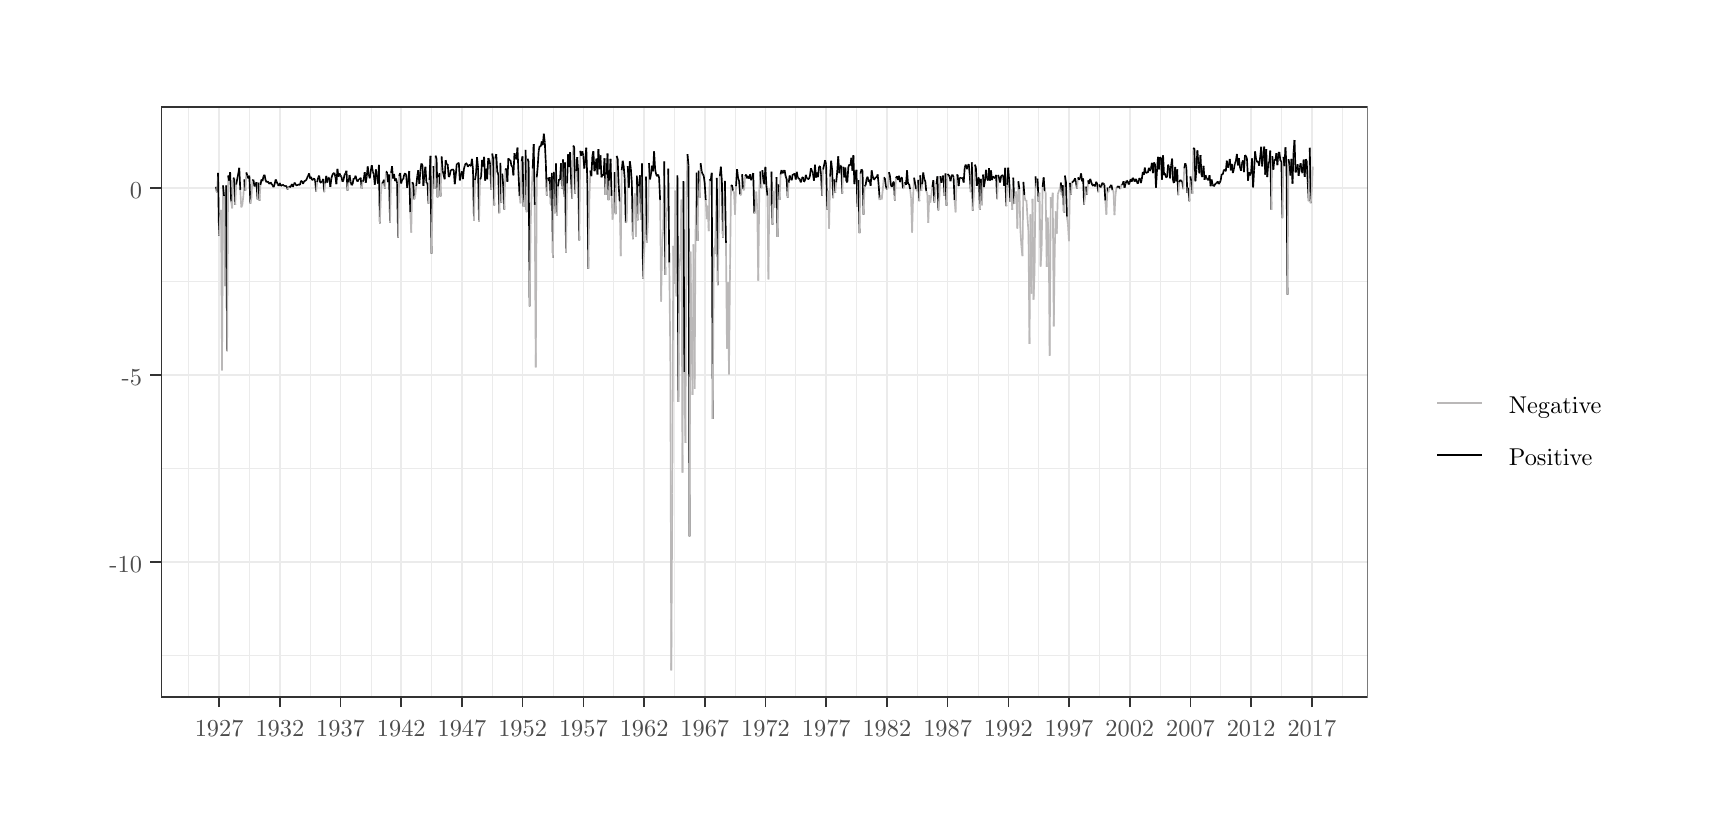
\begin{tikzpicture}[x=1.4pt,y=1.3pt]
\definecolor{fillColor}{RGB}{255,255,255}
\path[use as bounding box,fill=fillColor,fill opacity=0.00] (0,0) rectangle (426.79,216.81);
\begin{scope}
\path[clip] (  0.00,  0.00) rectangle (426.79,216.81);
\definecolor{drawColor}{RGB}{255,255,255}
\definecolor{fillColor}{RGB}{255,255,255}

\path[draw=drawColor,line width= 0.6pt,line join=round,line cap=round,fill=fillColor] (  0.00,  0.00) rectangle (426.79,216.81);
\end{scope}
\begin{scope}
\path[clip] ( 34.45, 30.72) rectangle (345.86,194.77);
\definecolor{fillColor}{RGB}{255,255,255}

\path[fill=fillColor] ( 34.45, 30.72) rectangle (345.86,194.77);
\definecolor{drawColor}{gray}{0.92}

\path[draw=drawColor,line width= 0.3pt,line join=round] ( 34.45, 42.33) --
	(345.86, 42.33);

\path[draw=drawColor,line width= 0.3pt,line join=round] ( 34.45, 94.30) --
	(345.86, 94.30);

\path[draw=drawColor,line width= 0.3pt,line join=round] ( 34.45,146.27) --
	(345.86,146.27);

\path[draw=drawColor,line width= 0.3pt,line join=round] ( 41.59, 30.72) --
	( 41.59,194.77);

\path[draw=drawColor,line width= 0.3pt,line join=round] ( 57.25, 30.72) --
	( 57.25,194.77);

\path[draw=drawColor,line width= 0.3pt,line join=round] ( 72.93, 30.72) --
	( 72.93,194.77);

\path[draw=drawColor,line width= 0.3pt,line join=round] ( 88.60, 30.72) --
	( 88.60,194.77);

\path[draw=drawColor,line width= 0.3pt,line join=round] (104.26, 30.72) --
	(104.26,194.77);

\path[draw=drawColor,line width= 0.3pt,line join=round] (119.93, 30.72) --
	(119.93,194.77);

\path[draw=drawColor,line width= 0.3pt,line join=round] (135.60, 30.72) --
	(135.60,194.77);

\path[draw=drawColor,line width= 0.3pt,line join=round] (151.27, 30.72) --
	(151.27,194.77);

\path[draw=drawColor,line width= 0.3pt,line join=round] (166.94, 30.72) --
	(166.94,194.77);

\path[draw=drawColor,line width= 0.3pt,line join=round] (182.61, 30.72) --
	(182.61,194.77);

\path[draw=drawColor,line width= 0.3pt,line join=round] (198.28, 30.72) --
	(198.28,194.77);

\path[draw=drawColor,line width= 0.3pt,line join=round] (213.95, 30.72) --
	(213.95,194.77);

\path[draw=drawColor,line width= 0.3pt,line join=round] (229.62, 30.72) --
	(229.62,194.77);

\path[draw=drawColor,line width= 0.3pt,line join=round] (245.28, 30.72) --
	(245.28,194.77);

\path[draw=drawColor,line width= 0.3pt,line join=round] (260.96, 30.72) --
	(260.96,194.77);

\path[draw=drawColor,line width= 0.3pt,line join=round] (276.63, 30.72) --
	(276.63,194.77);

\path[draw=drawColor,line width= 0.3pt,line join=round] (292.29, 30.72) --
	(292.29,194.77);

\path[draw=drawColor,line width= 0.3pt,line join=round] (307.96, 30.72) --
	(307.96,194.77);

\path[draw=drawColor,line width= 0.3pt,line join=round] (323.63, 30.72) --
	(323.63,194.77);

\path[draw=drawColor,line width= 0.3pt,line join=round] (339.30, 30.72) --
	(339.30,194.77);

\path[draw=drawColor,line width= 0.6pt,line join=round] ( 34.45, 68.32) --
	(345.86, 68.32);

\path[draw=drawColor,line width= 0.6pt,line join=round] ( 34.45,120.29) --
	(345.86,120.29);

\path[draw=drawColor,line width= 0.6pt,line join=round] ( 34.45,172.25) --
	(345.86,172.25);

\path[draw=drawColor,line width= 0.6pt,line join=round] ( 49.42, 30.72) --
	( 49.42,194.77);

\path[draw=drawColor,line width= 0.6pt,line join=round] ( 65.09, 30.72) --
	( 65.09,194.77);

\path[draw=drawColor,line width= 0.6pt,line join=round] ( 80.76, 30.72) --
	( 80.76,194.77);

\path[draw=drawColor,line width= 0.6pt,line join=round] ( 96.43, 30.72) --
	( 96.43,194.77);

\path[draw=drawColor,line width= 0.6pt,line join=round] (112.10, 30.72) --
	(112.10,194.77);

\path[draw=drawColor,line width= 0.6pt,line join=round] (127.76, 30.72) --
	(127.76,194.77);

\path[draw=drawColor,line width= 0.6pt,line join=round] (143.44, 30.72) --
	(143.44,194.77);

\path[draw=drawColor,line width= 0.6pt,line join=round] (159.11, 30.72) --
	(159.11,194.77);

\path[draw=drawColor,line width= 0.6pt,line join=round] (174.77, 30.72) --
	(174.77,194.77);

\path[draw=drawColor,line width= 0.6pt,line join=round] (190.44, 30.72) --
	(190.44,194.77);

\path[draw=drawColor,line width= 0.6pt,line join=round] (206.12, 30.72) --
	(206.12,194.77);

\path[draw=drawColor,line width= 0.6pt,line join=round] (221.78, 30.72) --
	(221.78,194.77);

\path[draw=drawColor,line width= 0.6pt,line join=round] (237.45, 30.72) --
	(237.45,194.77);

\path[draw=drawColor,line width= 0.6pt,line join=round] (253.12, 30.72) --
	(253.12,194.77);

\path[draw=drawColor,line width= 0.6pt,line join=round] (268.79, 30.72) --
	(268.79,194.77);

\path[draw=drawColor,line width= 0.6pt,line join=round] (284.46, 30.72) --
	(284.46,194.77);

\path[draw=drawColor,line width= 0.6pt,line join=round] (300.13, 30.72) --
	(300.13,194.77);

\path[draw=drawColor,line width= 0.6pt,line join=round] (315.79, 30.72) --
	(315.79,194.77);

\path[draw=drawColor,line width= 0.6pt,line join=round] (331.47, 30.72) --
	(331.47,194.77);
\definecolor{drawColor}{RGB}{0,0,0}

\path[draw=drawColor,line width= 0.6pt,line join=round] ( 48.61,172.56) -- ( 48.86,170.90);
\definecolor{drawColor}{RGB}{186,184,184}

\path[draw=drawColor,line width= 0.6pt,line join=round] ( 48.86,170.90) -- ( 49.13,176.47);
\definecolor{drawColor}{RGB}{0,0,0}

\path[draw=drawColor,line width= 0.6pt,line join=round] ( 49.13,176.47) -- ( 49.39,159.04);
\definecolor{drawColor}{RGB}{186,184,184}

\path[draw=drawColor,line width= 0.6pt,line join=round] ( 49.39,159.04) -- ( 49.65,163.94);

\path[draw=drawColor,line width= 0.6pt,line join=round] ( 49.65,163.94) -- ( 49.92,166.14);

\path[draw=drawColor,line width= 0.6pt,line join=round] ( 49.92,166.14) -- ( 50.16,121.56);

\path[draw=drawColor,line width= 0.6pt,line join=round] ( 50.16,121.56) -- ( 50.42,172.95);
\definecolor{drawColor}{RGB}{0,0,0}

\path[draw=drawColor,line width= 0.6pt,line join=round] ( 50.42,172.95) -- ( 50.68,170.00);
\definecolor{drawColor}{RGB}{186,184,184}

\path[draw=drawColor,line width= 0.6pt,line join=round] ( 50.68,170.00) -- ( 50.95,145.00);

\path[draw=drawColor,line width= 0.6pt,line join=round] ( 50.95,145.00) -- ( 51.21,172.96);
\definecolor{drawColor}{RGB}{0,0,0}

\path[draw=drawColor,line width= 0.6pt,line join=round] ( 51.21,172.96) -- ( 51.47,126.91);
\definecolor{drawColor}{RGB}{186,184,184}

\path[draw=drawColor,line width= 0.6pt,line join=round] ( 51.47,126.91) -- ( 51.74,175.72);
\definecolor{drawColor}{RGB}{0,0,0}

\path[draw=drawColor,line width= 0.6pt,line join=round] ( 51.74,175.72) -- ( 51.99,174.30);

\path[draw=drawColor,line width= 0.6pt,line join=round] ( 51.99,174.30) -- ( 52.26,176.63);

\path[draw=drawColor,line width= 0.6pt,line join=round] ( 52.26,176.63) -- ( 52.52,168.48);
\definecolor{drawColor}{RGB}{186,184,184}

\path[draw=drawColor,line width= 0.6pt,line join=round] ( 52.52,168.48) -- ( 52.78,166.57);

\path[draw=drawColor,line width= 0.6pt,line join=round] ( 52.78,166.57) -- ( 53.05,175.05);
\definecolor{drawColor}{RGB}{0,0,0}

\path[draw=drawColor,line width= 0.6pt,line join=round] ( 53.05,175.05) -- ( 53.30,174.90);

\path[draw=drawColor,line width= 0.6pt,line join=round] ( 53.30,174.90) -- ( 53.56,167.58);
\definecolor{drawColor}{RGB}{186,184,184}

\path[draw=drawColor,line width= 0.6pt,line join=round] ( 53.56,167.58) -- ( 53.82,173.19);
\definecolor{drawColor}{RGB}{0,0,0}

\path[draw=drawColor,line width= 0.6pt,line join=round] ( 53.82,173.19) -- ( 54.09,174.81);

\path[draw=drawColor,line width= 0.6pt,line join=round] ( 54.09,174.81) -- ( 54.35,176.14);

\path[draw=drawColor,line width= 0.6pt,line join=round] ( 54.35,176.14) -- ( 54.61,177.84);

\path[draw=drawColor,line width= 0.6pt,line join=round] ( 54.61,177.84) -- ( 54.88,171.70);
\definecolor{drawColor}{RGB}{186,184,184}

\path[draw=drawColor,line width= 0.6pt,line join=round] ( 54.88,171.70) -- ( 55.13,166.88);

\path[draw=drawColor,line width= 0.6pt,line join=round] ( 55.13,166.88) -- ( 55.40,167.50);

\path[draw=drawColor,line width= 0.6pt,line join=round] ( 55.40,167.50) -- ( 55.66,169.98);

\path[draw=drawColor,line width= 0.6pt,line join=round] ( 55.66,169.98) -- ( 55.92,174.64);
\definecolor{drawColor}{RGB}{0,0,0}

\path[draw=drawColor,line width= 0.6pt,line join=round] ( 55.92,174.64) -- ( 56.19,171.48);
\definecolor{drawColor}{RGB}{186,184,184}

\path[draw=drawColor,line width= 0.6pt,line join=round] ( 56.19,171.48) -- ( 56.43,176.56);
\definecolor{drawColor}{RGB}{0,0,0}

\path[draw=drawColor,line width= 0.6pt,line join=round] ( 56.43,176.56) -- ( 56.70,175.71);

\path[draw=drawColor,line width= 0.6pt,line join=round] ( 56.70,175.71) -- ( 56.95,174.90);

\path[draw=drawColor,line width= 0.6pt,line join=round] ( 56.95,174.90) -- ( 57.22,175.66);

\path[draw=drawColor,line width= 0.6pt,line join=round] ( 57.22,175.66) -- ( 57.48,167.88);
\definecolor{drawColor}{RGB}{186,184,184}

\path[draw=drawColor,line width= 0.6pt,line join=round] ( 57.48,167.88) -- ( 57.74,169.33);

\path[draw=drawColor,line width= 0.6pt,line join=round] ( 57.74,169.33) -- ( 58.01,174.35);
\definecolor{drawColor}{RGB}{0,0,0}

\path[draw=drawColor,line width= 0.6pt,line join=round] ( 58.01,174.35) -- ( 58.27,174.53);

\path[draw=drawColor,line width= 0.6pt,line join=round] ( 58.27,174.53) -- ( 58.53,172.69);

\path[draw=drawColor,line width= 0.6pt,line join=round] ( 58.53,172.69) -- ( 58.79,173.00);

\path[draw=drawColor,line width= 0.6pt,line join=round] ( 58.79,173.00) -- ( 59.06,173.86);

\path[draw=drawColor,line width= 0.6pt,line join=round] ( 59.06,173.86) -- ( 59.32,169.07);
\definecolor{drawColor}{RGB}{186,184,184}

\path[draw=drawColor,line width= 0.6pt,line join=round] ( 59.32,169.07) -- ( 59.56,173.76);
\definecolor{drawColor}{RGB}{0,0,0}

\path[draw=drawColor,line width= 0.6pt,line join=round] ( 59.56,173.76) -- ( 59.83,168.75);
\definecolor{drawColor}{RGB}{186,184,184}

\path[draw=drawColor,line width= 0.6pt,line join=round] ( 59.83,168.75) -- ( 60.09,173.13);
\definecolor{drawColor}{RGB}{0,0,0}

\path[draw=drawColor,line width= 0.6pt,line join=round] ( 60.09,173.13) -- ( 60.35,174.63);

\path[draw=drawColor,line width= 0.6pt,line join=round] ( 60.35,174.63) -- ( 60.61,174.16);

\path[draw=drawColor,line width= 0.6pt,line join=round] ( 60.61,174.16) -- ( 60.87,175.50);

\path[draw=drawColor,line width= 0.6pt,line join=round] ( 60.87,175.50) -- ( 61.14,175.91);

\path[draw=drawColor,line width= 0.6pt,line join=round] ( 61.14,175.91) -- ( 61.40,174.42);

\path[draw=drawColor,line width= 0.6pt,line join=round] ( 61.40,174.42) -- ( 61.66,173.82);

\path[draw=drawColor,line width= 0.6pt,line join=round] ( 61.66,173.82) -- ( 61.92,174.12);

\path[draw=drawColor,line width= 0.6pt,line join=round] ( 61.92,174.12) -- ( 62.19,173.71);

\path[draw=drawColor,line width= 0.6pt,line join=round] ( 62.19,173.71) -- ( 62.45,173.35);

\path[draw=drawColor,line width= 0.6pt,line join=round] ( 62.45,173.35) -- ( 62.69,173.87);

\path[draw=drawColor,line width= 0.6pt,line join=round] ( 62.69,173.87) -- ( 62.96,173.33);

\path[draw=drawColor,line width= 0.6pt,line join=round] ( 62.96,173.33) -- ( 63.22,173.04);

\path[draw=drawColor,line width= 0.6pt,line join=round] ( 63.22,173.04) -- ( 63.48,172.47);

\path[draw=drawColor,line width= 0.6pt,line join=round] ( 63.48,172.47) -- ( 63.74,173.31);

\path[draw=drawColor,line width= 0.6pt,line join=round] ( 63.74,173.31) -- ( 64.01,174.60);

\path[draw=drawColor,line width= 0.6pt,line join=round] ( 64.01,174.60) -- ( 64.27,174.02);

\path[draw=drawColor,line width= 0.6pt,line join=round] ( 64.27,174.02) -- ( 64.53,173.25);

\path[draw=drawColor,line width= 0.6pt,line join=round] ( 64.53,173.25) -- ( 64.80,172.83);

\path[draw=drawColor,line width= 0.6pt,line join=round] ( 64.80,172.83) -- ( 65.05,173.64);

\path[draw=drawColor,line width= 0.6pt,line join=round] ( 65.05,173.64) -- ( 65.32,172.81);

\path[draw=drawColor,line width= 0.6pt,line join=round] ( 65.32,172.81) -- ( 65.59,173.02);

\path[draw=drawColor,line width= 0.6pt,line join=round] ( 65.59,173.02) -- ( 65.83,173.19);

\path[draw=drawColor,line width= 0.6pt,line join=round] ( 65.83,173.19) -- ( 66.10,172.88);

\path[draw=drawColor,line width= 0.6pt,line join=round] ( 66.10,172.88) -- ( 66.36,172.79);

\path[draw=drawColor,line width= 0.6pt,line join=round] ( 66.36,172.79) -- ( 66.62,172.83);

\path[draw=drawColor,line width= 0.6pt,line join=round] ( 66.62,172.83) -- ( 66.88,172.65);

\path[draw=drawColor,line width= 0.6pt,line join=round] ( 66.88,172.65) -- ( 67.15,171.78);
\definecolor{drawColor}{RGB}{186,184,184}

\path[draw=drawColor,line width= 0.6pt,line join=round] ( 67.15,171.78) -- ( 67.41,172.72);
\definecolor{drawColor}{RGB}{0,0,0}

\path[draw=drawColor,line width= 0.6pt,line join=round] ( 67.41,172.72) -- ( 67.67,172.50);

\path[draw=drawColor,line width= 0.6pt,line join=round] ( 67.67,172.50) -- ( 67.94,172.67);

\path[draw=drawColor,line width= 0.6pt,line join=round] ( 67.94,172.67) -- ( 68.19,173.35);

\path[draw=drawColor,line width= 0.6pt,line join=round] ( 68.19,173.35) -- ( 68.46,172.54);

\path[draw=drawColor,line width= 0.6pt,line join=round] ( 68.46,172.54) -- ( 68.73,173.45);

\path[draw=drawColor,line width= 0.6pt,line join=round] ( 68.73,173.45) -- ( 68.97,173.71);

\path[draw=drawColor,line width= 0.6pt,line join=round] ( 68.97,173.71) -- ( 69.23,172.97);

\path[draw=drawColor,line width= 0.6pt,line join=round] ( 69.23,172.97) -- ( 69.49,173.03);

\path[draw=drawColor,line width= 0.6pt,line join=round] ( 69.49,173.03) -- ( 69.75,173.06);

\path[draw=drawColor,line width= 0.6pt,line join=round] ( 69.75,173.06) -- ( 70.01,173.29);

\path[draw=drawColor,line width= 0.6pt,line join=round] ( 70.01,173.29) -- ( 70.28,173.07);

\path[draw=drawColor,line width= 0.6pt,line join=round] ( 70.28,173.07) -- ( 70.54,174.25);

\path[draw=drawColor,line width= 0.6pt,line join=round] ( 70.54,174.25) -- ( 70.80,174.10);

\path[draw=drawColor,line width= 0.6pt,line join=round] ( 70.80,174.10) -- ( 71.07,173.40);

\path[draw=drawColor,line width= 0.6pt,line join=round] ( 71.07,173.40) -- ( 71.33,174.05);

\path[draw=drawColor,line width= 0.6pt,line join=round] ( 71.33,174.05) -- ( 71.59,174.28);

\path[draw=drawColor,line width= 0.6pt,line join=round] ( 71.59,174.28) -- ( 71.86,174.33);

\path[draw=drawColor,line width= 0.6pt,line join=round] ( 71.86,174.33) -- ( 72.10,174.98);

\path[draw=drawColor,line width= 0.6pt,line join=round] ( 72.10,174.98) -- ( 72.36,175.60);

\path[draw=drawColor,line width= 0.6pt,line join=round] ( 72.36,175.60) -- ( 72.62,176.30);

\path[draw=drawColor,line width= 0.6pt,line join=round] ( 72.62,176.30) -- ( 72.89,174.90);

\path[draw=drawColor,line width= 0.6pt,line join=round] ( 72.89,174.90) -- ( 73.14,175.33);

\path[draw=drawColor,line width= 0.6pt,line join=round] ( 73.14,175.33) -- ( 73.41,174.43);

\path[draw=drawColor,line width= 0.6pt,line join=round] ( 73.41,174.43) -- ( 73.68,174.63);

\path[draw=drawColor,line width= 0.6pt,line join=round] ( 73.68,174.63) -- ( 73.93,174.94);

\path[draw=drawColor,line width= 0.6pt,line join=round] ( 73.93,174.94) -- ( 74.20,174.29);

\path[draw=drawColor,line width= 0.6pt,line join=round] ( 74.20,174.29) -- ( 74.46,171.18);
\definecolor{drawColor}{RGB}{186,184,184}

\path[draw=drawColor,line width= 0.6pt,line join=round] ( 74.46,171.18) -- ( 74.72,173.90);
\definecolor{drawColor}{RGB}{0,0,0}

\path[draw=drawColor,line width= 0.6pt,line join=round] ( 74.72,173.90) -- ( 74.99,175.17);

\path[draw=drawColor,line width= 0.6pt,line join=round] ( 74.99,175.17) -- ( 75.23,175.69);

\path[draw=drawColor,line width= 0.6pt,line join=round] ( 75.23,175.69) -- ( 75.49,173.78);

\path[draw=drawColor,line width= 0.6pt,line join=round] ( 75.49,173.78) -- ( 75.75,173.75);

\path[draw=drawColor,line width= 0.6pt,line join=round] ( 75.75,173.75) -- ( 76.02,174.04);

\path[draw=drawColor,line width= 0.6pt,line join=round] ( 76.02,174.04) -- ( 76.28,174.75);

\path[draw=drawColor,line width= 0.6pt,line join=round] ( 76.28,174.75) -- ( 76.54,171.12);
\definecolor{drawColor}{RGB}{186,184,184}

\path[draw=drawColor,line width= 0.6pt,line join=round] ( 76.54,171.12) -- ( 76.81,173.53);
\definecolor{drawColor}{RGB}{0,0,0}

\path[draw=drawColor,line width= 0.6pt,line join=round] ( 76.81,173.53) -- ( 77.07,175.61);

\path[draw=drawColor,line width= 0.6pt,line join=round] ( 77.07,175.61) -- ( 77.33,173.76);

\path[draw=drawColor,line width= 0.6pt,line join=round] ( 77.33,173.76) -- ( 77.59,175.13);

\path[draw=drawColor,line width= 0.6pt,line join=round] ( 77.59,175.13) -- ( 77.85,175.09);

\path[draw=drawColor,line width= 0.6pt,line join=round] ( 77.85,175.09) -- ( 78.12,172.54);

\path[draw=drawColor,line width= 0.6pt,line join=round] ( 78.12,172.54) -- ( 78.37,174.86);

\path[draw=drawColor,line width= 0.6pt,line join=round] ( 78.37,174.86) -- ( 78.64,175.87);

\path[draw=drawColor,line width= 0.6pt,line join=round] ( 78.64,175.87) -- ( 78.89,176.29);

\path[draw=drawColor,line width= 0.6pt,line join=round] ( 78.89,176.29) -- ( 79.16,176.44);

\path[draw=drawColor,line width= 0.6pt,line join=round] ( 79.16,176.44) -- ( 79.42,175.40);

\path[draw=drawColor,line width= 0.6pt,line join=round] ( 79.42,175.40) -- ( 79.68,173.30);

\path[draw=drawColor,line width= 0.6pt,line join=round] ( 79.68,173.30) -- ( 79.95,177.56);

\path[draw=drawColor,line width= 0.6pt,line join=round] ( 79.95,177.56) -- ( 80.21,175.34);

\path[draw=drawColor,line width= 0.6pt,line join=round] ( 80.21,175.34) -- ( 80.47,176.30);

\path[draw=drawColor,line width= 0.6pt,line join=round] ( 80.47,176.30) -- ( 80.73,175.70);

\path[draw=drawColor,line width= 0.6pt,line join=round] ( 80.73,175.70) -- ( 80.99,175.38);

\path[draw=drawColor,line width= 0.6pt,line join=round] ( 80.99,175.38) -- ( 81.26,173.98);

\path[draw=drawColor,line width= 0.6pt,line join=round] ( 81.26,173.98) -- ( 81.50,174.41);

\path[draw=drawColor,line width= 0.6pt,line join=round] ( 81.50,174.41) -- ( 81.77,175.89);

\path[draw=drawColor,line width= 0.6pt,line join=round] ( 81.77,175.89) -- ( 82.02,176.26);

\path[draw=drawColor,line width= 0.6pt,line join=round] ( 82.02,176.26) -- ( 82.29,177.03);

\path[draw=drawColor,line width= 0.6pt,line join=round] ( 82.29,177.03) -- ( 82.55,171.52);
\definecolor{drawColor}{RGB}{186,184,184}

\path[draw=drawColor,line width= 0.6pt,line join=round] ( 82.55,171.52) -- ( 82.81,173.79);
\definecolor{drawColor}{RGB}{0,0,0}

\path[draw=drawColor,line width= 0.6pt,line join=round] ( 82.81,173.79) -- ( 83.08,175.84);

\path[draw=drawColor,line width= 0.6pt,line join=round] ( 83.08,175.84) -- ( 83.34,174.05);

\path[draw=drawColor,line width= 0.6pt,line join=round] ( 83.34,174.05) -- ( 83.60,173.04);

\path[draw=drawColor,line width= 0.6pt,line join=round] ( 83.60,173.04) -- ( 83.86,173.28);

\path[draw=drawColor,line width= 0.6pt,line join=round] ( 83.86,173.28) -- ( 84.13,174.94);

\path[draw=drawColor,line width= 0.6pt,line join=round] ( 84.13,174.94) -- ( 84.39,174.76);

\path[draw=drawColor,line width= 0.6pt,line join=round] ( 84.39,174.76) -- ( 84.63,175.66);

\path[draw=drawColor,line width= 0.6pt,line join=round] ( 84.63,175.66) -- ( 84.90,174.50);

\path[draw=drawColor,line width= 0.6pt,line join=round] ( 84.90,174.50) -- ( 85.16,174.00);

\path[draw=drawColor,line width= 0.6pt,line join=round] ( 85.16,174.00) -- ( 85.42,174.72);

\path[draw=drawColor,line width= 0.6pt,line join=round] ( 85.42,174.72) -- ( 85.68,174.63);

\path[draw=drawColor,line width= 0.6pt,line join=round] ( 85.68,174.63) -- ( 85.95,175.10);

\path[draw=drawColor,line width= 0.6pt,line join=round] ( 85.95,175.10) -- ( 86.21,172.01);
\definecolor{drawColor}{RGB}{186,184,184}

\path[draw=drawColor,line width= 0.6pt,line join=round] ( 86.21,172.01) -- ( 86.47,174.03);
\definecolor{drawColor}{RGB}{0,0,0}

\path[draw=drawColor,line width= 0.6pt,line join=round] ( 86.47,174.03) -- ( 86.73,174.50);

\path[draw=drawColor,line width= 0.6pt,line join=round] ( 86.73,174.50) -- ( 86.99,176.64);

\path[draw=drawColor,line width= 0.6pt,line join=round] ( 86.99,176.64) -- ( 87.26,173.72);

\path[draw=drawColor,line width= 0.6pt,line join=round] ( 87.26,173.72) -- ( 87.52,175.41);

\path[draw=drawColor,line width= 0.6pt,line join=round] ( 87.52,175.41) -- ( 87.76,178.22);

\path[draw=drawColor,line width= 0.6pt,line join=round] ( 87.76,178.22) -- ( 88.03,176.08);

\path[draw=drawColor,line width= 0.6pt,line join=round] ( 88.03,176.08) -- ( 88.29,174.95);

\path[draw=drawColor,line width= 0.6pt,line join=round] ( 88.29,174.95) -- ( 88.55,176.90);

\path[draw=drawColor,line width= 0.6pt,line join=round] ( 88.55,176.90) -- ( 88.81,178.58);

\path[draw=drawColor,line width= 0.6pt,line join=round] ( 88.81,178.58) -- ( 89.08,176.82);

\path[draw=drawColor,line width= 0.6pt,line join=round] ( 89.08,176.82) -- ( 89.34,175.99);

\path[draw=drawColor,line width= 0.6pt,line join=round] ( 89.34,175.99) -- ( 89.60,173.16);

\path[draw=drawColor,line width= 0.6pt,line join=round] ( 89.60,173.16) -- ( 89.87,177.40);

\path[draw=drawColor,line width= 0.6pt,line join=round] ( 89.87,177.40) -- ( 90.12,175.90);

\path[draw=drawColor,line width= 0.6pt,line join=round] ( 90.12,175.90) -- ( 90.39,173.48);

\path[draw=drawColor,line width= 0.6pt,line join=round] ( 90.39,173.48) -- ( 90.66,178.64);

\path[draw=drawColor,line width= 0.6pt,line join=round] ( 90.66,178.64) -- ( 90.90,162.40);
\definecolor{drawColor}{RGB}{186,184,184}

\path[draw=drawColor,line width= 0.6pt,line join=round] ( 90.90,162.40) -- ( 91.17,170.48);

\path[draw=drawColor,line width= 0.6pt,line join=round] ( 91.17,170.48) -- ( 91.43,173.76);
\definecolor{drawColor}{RGB}{0,0,0}

\path[draw=drawColor,line width= 0.6pt,line join=round] ( 91.43,173.76) -- ( 91.69,173.69);

\path[draw=drawColor,line width= 0.6pt,line join=round] ( 91.69,173.69) -- ( 91.95,174.53);

\path[draw=drawColor,line width= 0.6pt,line join=round] ( 91.95,174.53) -- ( 92.22,172.09);
\definecolor{drawColor}{RGB}{186,184,184}

\path[draw=drawColor,line width= 0.6pt,line join=round] ( 92.22,172.09) -- ( 92.48,176.77);
\definecolor{drawColor}{RGB}{0,0,0}

\path[draw=drawColor,line width= 0.6pt,line join=round] ( 92.48,176.77) -- ( 92.74,176.74);

\path[draw=drawColor,line width= 0.6pt,line join=round] ( 92.74,176.74) -- ( 93.01,173.88);

\path[draw=drawColor,line width= 0.6pt,line join=round] ( 93.01,173.88) -- ( 93.26,175.98);

\path[draw=drawColor,line width= 0.6pt,line join=round] ( 93.26,175.98) -- ( 93.53,162.67);
\definecolor{drawColor}{RGB}{186,184,184}

\path[draw=drawColor,line width= 0.6pt,line join=round] ( 93.53,162.67) -- ( 93.80,176.42);
\definecolor{drawColor}{RGB}{0,0,0}

\path[draw=drawColor,line width= 0.6pt,line join=round] ( 93.80,176.42) -- ( 94.04,178.29);

\path[draw=drawColor,line width= 0.6pt,line join=round] ( 94.04,178.29) -- ( 94.30,174.90);

\path[draw=drawColor,line width= 0.6pt,line join=round] ( 94.30,174.90) -- ( 94.56,176.13);

\path[draw=drawColor,line width= 0.6pt,line join=round] ( 94.56,176.13) -- ( 94.83,174.18);

\path[draw=drawColor,line width= 0.6pt,line join=round] ( 94.83,174.18) -- ( 95.08,174.88);

\path[draw=drawColor,line width= 0.6pt,line join=round] ( 95.08,174.88) -- ( 95.35,173.53);

\path[draw=drawColor,line width= 0.6pt,line join=round] ( 95.35,173.53) -- ( 95.61,158.47);
\definecolor{drawColor}{RGB}{186,184,184}

\path[draw=drawColor,line width= 0.6pt,line join=round] ( 95.61,158.47) -- ( 95.87,175.63);
\definecolor{drawColor}{RGB}{0,0,0}

\path[draw=drawColor,line width= 0.6pt,line join=round] ( 95.87,175.63) -- ( 96.14,176.40);

\path[draw=drawColor,line width= 0.6pt,line join=round] ( 96.14,176.40) -- ( 96.40,173.50);

\path[draw=drawColor,line width= 0.6pt,line join=round] ( 96.40,173.50) -- ( 96.66,174.59);

\path[draw=drawColor,line width= 0.6pt,line join=round] ( 96.66,174.59) -- ( 96.93,174.60);

\path[draw=drawColor,line width= 0.6pt,line join=round] ( 96.93,174.60) -- ( 97.17,175.96);

\path[draw=drawColor,line width= 0.6pt,line join=round] ( 97.17,175.96) -- ( 97.43,176.35);

\path[draw=drawColor,line width= 0.6pt,line join=round] ( 97.43,176.35) -- ( 97.69,175.89);

\path[draw=drawColor,line width= 0.6pt,line join=round] ( 97.69,175.89) -- ( 97.96,172.30);

\path[draw=drawColor,line width= 0.6pt,line join=round] ( 97.96,172.30) -- ( 98.21,174.51);

\path[draw=drawColor,line width= 0.6pt,line join=round] ( 98.21,174.51) -- ( 98.48,176.96);

\path[draw=drawColor,line width= 0.6pt,line join=round] ( 98.48,176.96) -- ( 98.75,165.53);
\definecolor{drawColor}{RGB}{186,184,184}

\path[draw=drawColor,line width= 0.6pt,line join=round] ( 98.75,165.53) -- ( 99.00,159.82);

\path[draw=drawColor,line width= 0.6pt,line join=round] ( 99.00,159.82) -- ( 99.27,173.86);
\definecolor{drawColor}{RGB}{0,0,0}

\path[draw=drawColor,line width= 0.6pt,line join=round] ( 99.27,173.86) -- ( 99.53,173.38);

\path[draw=drawColor,line width= 0.6pt,line join=round] ( 99.53,173.38) -- ( 99.79,169.11);
\definecolor{drawColor}{RGB}{186,184,184}

\path[draw=drawColor,line width= 0.6pt,line join=round] ( 99.79,169.11) -- (100.06,170.19);

\path[draw=drawColor,line width= 0.6pt,line join=round] (100.06,170.19) -- (100.30,172.83);
\definecolor{drawColor}{RGB}{0,0,0}

\path[draw=drawColor,line width= 0.6pt,line join=round] (100.30,172.83) -- (100.57,175.69);

\path[draw=drawColor,line width= 0.6pt,line join=round] (100.57,175.69) -- (100.82,177.19);

\path[draw=drawColor,line width= 0.6pt,line join=round] (100.82,177.19) -- (101.09,173.41);

\path[draw=drawColor,line width= 0.6pt,line join=round] (101.09,173.41) -- (101.35,176.85);

\path[draw=drawColor,line width= 0.6pt,line join=round] (101.35,176.85) -- (101.61,179.04);

\path[draw=drawColor,line width= 0.6pt,line join=round] (101.61,179.04) -- (101.88,178.62);

\path[draw=drawColor,line width= 0.6pt,line join=round] (101.88,178.62) -- (102.14,172.82);

\path[draw=drawColor,line width= 0.6pt,line join=round] (102.14,172.82) -- (102.40,176.34);

\path[draw=drawColor,line width= 0.6pt,line join=round] (102.40,176.34) -- (102.66,178.14);

\path[draw=drawColor,line width= 0.6pt,line join=round] (102.66,178.14) -- (102.93,173.61);

\path[draw=drawColor,line width= 0.6pt,line join=round] (102.93,173.61) -- (103.19,173.67);

\path[draw=drawColor,line width= 0.6pt,line join=round] (103.19,173.67) -- (103.44,167.94);
\definecolor{drawColor}{RGB}{186,184,184}

\path[draw=drawColor,line width= 0.6pt,line join=round] (103.44,167.94) -- (103.71,174.48);
\definecolor{drawColor}{RGB}{0,0,0}

\path[draw=drawColor,line width= 0.6pt,line join=round] (103.71,174.48) -- (103.96,181.16);

\path[draw=drawColor,line width= 0.6pt,line join=round] (103.96,181.16) -- (104.23,153.99);
\definecolor{drawColor}{RGB}{186,184,184}

\path[draw=drawColor,line width= 0.6pt,line join=round] (104.23,153.99) -- (104.49,169.19);

\path[draw=drawColor,line width= 0.6pt,line join=round] (104.49,169.19) -- (104.75,178.32);
\definecolor{drawColor}{RGB}{0,0,0}

\path[draw=drawColor,line width= 0.6pt,line join=round] (104.75,178.32) -- (105.02,171.99);
\definecolor{drawColor}{RGB}{186,184,184}

\path[draw=drawColor,line width= 0.6pt,line join=round] (105.02,171.99) -- (105.28,181.24);
\definecolor{drawColor}{RGB}{0,0,0}

\path[draw=drawColor,line width= 0.6pt,line join=round] (105.28,181.24) -- (105.54,180.35);

\path[draw=drawColor,line width= 0.6pt,line join=round] (105.54,180.35) -- (105.80,169.66);
\definecolor{drawColor}{RGB}{186,184,184}

\path[draw=drawColor,line width= 0.6pt,line join=round] (105.80,169.66) -- (106.07,175.33);
\definecolor{drawColor}{RGB}{0,0,0}

\path[draw=drawColor,line width= 0.6pt,line join=round] (106.07,175.33) -- (106.33,176.37);

\path[draw=drawColor,line width= 0.6pt,line join=round] (106.33,176.37) -- (106.57,169.91);
\definecolor{drawColor}{RGB}{186,184,184}

\path[draw=drawColor,line width= 0.6pt,line join=round] (106.57,169.91) -- (106.84,181.02);
\definecolor{drawColor}{RGB}{0,0,0}

\path[draw=drawColor,line width= 0.6pt,line join=round] (106.84,181.02) -- (107.09,177.06);

\path[draw=drawColor,line width= 0.6pt,line join=round] (107.09,177.06) -- (107.36,175.92);

\path[draw=drawColor,line width= 0.6pt,line join=round] (107.36,175.92) -- (107.62,174.68);

\path[draw=drawColor,line width= 0.6pt,line join=round] (107.62,174.68) -- (107.88,180.00);

\path[draw=drawColor,line width= 0.6pt,line join=round] (107.88,180.00) -- (108.15,178.77);

\path[draw=drawColor,line width= 0.6pt,line join=round] (108.15,178.77) -- (108.41,178.85);

\path[draw=drawColor,line width= 0.6pt,line join=round] (108.41,178.85) -- (108.67,175.30);

\path[draw=drawColor,line width= 0.6pt,line join=round] (108.67,175.30) -- (108.93,175.71);

\path[draw=drawColor,line width= 0.6pt,line join=round] (108.93,175.71) -- (109.20,177.29);

\path[draw=drawColor,line width= 0.6pt,line join=round] (109.20,177.29) -- (109.46,177.23);

\path[draw=drawColor,line width= 0.6pt,line join=round] (109.46,177.23) -- (109.70,177.49);

\path[draw=drawColor,line width= 0.6pt,line join=round] (109.70,177.49) -- (109.97,177.20);

\path[draw=drawColor,line width= 0.6pt,line join=round] (109.97,177.20) -- (110.23,173.33);

\path[draw=drawColor,line width= 0.6pt,line join=round] (110.23,173.33) -- (110.49,175.78);

\path[draw=drawColor,line width= 0.6pt,line join=round] (110.49,175.78) -- (110.75,179.03);

\path[draw=drawColor,line width= 0.6pt,line join=round] (110.75,179.03) -- (111.02,178.94);

\path[draw=drawColor,line width= 0.6pt,line join=round] (111.02,178.94) -- (111.28,179.29);

\path[draw=drawColor,line width= 0.6pt,line join=round] (111.28,179.29) -- (111.54,174.35);

\path[draw=drawColor,line width= 0.6pt,line join=round] (111.54,174.35) -- (111.81,175.89);

\path[draw=drawColor,line width= 0.6pt,line join=round] (111.81,175.89) -- (112.06,176.88);

\path[draw=drawColor,line width= 0.6pt,line join=round] (112.06,176.88) -- (112.33,174.73);

\path[draw=drawColor,line width= 0.6pt,line join=round] (112.33,174.73) -- (112.59,177.48);

\path[draw=drawColor,line width= 0.6pt,line join=round] (112.59,177.48) -- (112.83,178.49);

\path[draw=drawColor,line width= 0.6pt,line join=round] (112.83,178.49) -- (113.10,179.15);

\path[draw=drawColor,line width= 0.6pt,line join=round] (113.10,179.15) -- (113.36,179.02);

\path[draw=drawColor,line width= 0.6pt,line join=round] (113.36,179.02) -- (113.62,178.13);

\path[draw=drawColor,line width= 0.6pt,line join=round] (113.62,178.13) -- (113.88,178.68);

\path[draw=drawColor,line width= 0.6pt,line join=round] (113.88,178.68) -- (114.15,178.64);

\path[draw=drawColor,line width= 0.6pt,line join=round] (114.15,178.64) -- (114.41,178.32);

\path[draw=drawColor,line width= 0.6pt,line join=round] (114.41,178.32) -- (114.67,180.33);

\path[draw=drawColor,line width= 0.6pt,line join=round] (114.67,180.33) -- (114.94,177.39);

\path[draw=drawColor,line width= 0.6pt,line join=round] (114.94,177.39) -- (115.19,163.09);
\definecolor{drawColor}{RGB}{186,184,184}

\path[draw=drawColor,line width= 0.6pt,line join=round] (115.19,163.09) -- (115.46,174.48);
\definecolor{drawColor}{RGB}{0,0,0}

\path[draw=drawColor,line width= 0.6pt,line join=round] (115.46,174.48) -- (115.73,176.36);

\path[draw=drawColor,line width= 0.6pt,line join=round] (115.73,176.36) -- (115.98,180.79);

\path[draw=drawColor,line width= 0.6pt,line join=round] (115.98,180.79) -- (116.24,177.98);

\path[draw=drawColor,line width= 0.6pt,line join=round] (116.24,177.98) -- (116.50,162.83);
\definecolor{drawColor}{RGB}{186,184,184}

\path[draw=drawColor,line width= 0.6pt,line join=round] (116.50,162.83) -- (116.76,174.64);
\definecolor{drawColor}{RGB}{0,0,0}

\path[draw=drawColor,line width= 0.6pt,line join=round] (116.76,174.64) -- (117.02,175.22);

\path[draw=drawColor,line width= 0.6pt,line join=round] (117.02,175.22) -- (117.29,180.03);

\path[draw=drawColor,line width= 0.6pt,line join=round] (117.29,180.03) -- (117.55,178.23);

\path[draw=drawColor,line width= 0.6pt,line join=round] (117.55,178.23) -- (117.81,180.91);

\path[draw=drawColor,line width= 0.6pt,line join=round] (117.81,180.91) -- (118.08,174.30);

\path[draw=drawColor,line width= 0.6pt,line join=round] (118.08,174.30) -- (118.33,177.62);

\path[draw=drawColor,line width= 0.6pt,line join=round] (118.33,177.62) -- (118.60,174.68);

\path[draw=drawColor,line width= 0.6pt,line join=round] (118.60,174.68) -- (118.87,180.51);

\path[draw=drawColor,line width= 0.6pt,line join=round] (118.87,180.51) -- (119.11,180.17);

\path[draw=drawColor,line width= 0.6pt,line join=round] (119.11,180.17) -- (119.37,178.82);

\path[draw=drawColor,line width= 0.6pt,line join=round] (119.37,178.82) -- (119.63,171.83);
\definecolor{drawColor}{RGB}{186,184,184}

\path[draw=drawColor,line width= 0.6pt,line join=round] (119.63,171.83) -- (119.90,181.82);
\definecolor{drawColor}{RGB}{0,0,0}

\path[draw=drawColor,line width= 0.6pt,line join=round] (119.90,181.82) -- (120.15,180.34);

\path[draw=drawColor,line width= 0.6pt,line join=round] (120.15,180.34) -- (120.42,167.42);
\definecolor{drawColor}{RGB}{186,184,184}

\path[draw=drawColor,line width= 0.6pt,line join=round] (120.42,167.42) -- (120.69,180.46);
\definecolor{drawColor}{RGB}{0,0,0}

\path[draw=drawColor,line width= 0.6pt,line join=round] (120.69,180.46) -- (120.94,181.66);

\path[draw=drawColor,line width= 0.6pt,line join=round] (120.94,181.66) -- (121.21,176.72);

\path[draw=drawColor,line width= 0.6pt,line join=round] (121.21,176.72) -- (121.47,176.16);

\path[draw=drawColor,line width= 0.6pt,line join=round] (121.47,176.16) -- (121.73,165.23);
\definecolor{drawColor}{RGB}{186,184,184}

\path[draw=drawColor,line width= 0.6pt,line join=round] (121.73,165.23) -- (122.00,179.25);
\definecolor{drawColor}{RGB}{0,0,0}

\path[draw=drawColor,line width= 0.6pt,line join=round] (122.00,179.25) -- (122.24,168.18);
\definecolor{drawColor}{RGB}{186,184,184}

\path[draw=drawColor,line width= 0.6pt,line join=round] (122.24,168.18) -- (122.50,176.22);
\definecolor{drawColor}{RGB}{0,0,0}

\path[draw=drawColor,line width= 0.6pt,line join=round] (122.50,176.22) -- (122.76,172.66);

\path[draw=drawColor,line width= 0.6pt,line join=round] (122.76,172.66) -- (123.03,166.24);
\definecolor{drawColor}{RGB}{186,184,184}

\path[draw=drawColor,line width= 0.6pt,line join=round] (123.03,166.24) -- (123.29,177.30);
\definecolor{drawColor}{RGB}{0,0,0}

\path[draw=drawColor,line width= 0.6pt,line join=round] (123.29,177.30) -- (123.55,177.65);

\path[draw=drawColor,line width= 0.6pt,line join=round] (123.55,177.65) -- (123.82,173.97);

\path[draw=drawColor,line width= 0.6pt,line join=round] (123.82,173.97) -- (124.07,180.51);

\path[draw=drawColor,line width= 0.6pt,line join=round] (124.07,180.51) -- (124.34,179.94);

\path[draw=drawColor,line width= 0.6pt,line join=round] (124.34,179.94) -- (124.60,180.04);

\path[draw=drawColor,line width= 0.6pt,line join=round] (124.60,180.04) -- (124.86,178.35);

\path[draw=drawColor,line width= 0.6pt,line join=round] (124.86,178.35) -- (125.13,178.22);

\path[draw=drawColor,line width= 0.6pt,line join=round] (125.13,178.22) -- (125.37,175.76);

\path[draw=drawColor,line width= 0.6pt,line join=round] (125.37,175.76) -- (125.64,181.90);

\path[draw=drawColor,line width= 0.6pt,line join=round] (125.64,181.90) -- (125.89,180.97);

\path[draw=drawColor,line width= 0.6pt,line join=round] (125.89,180.97) -- (126.16,180.20);

\path[draw=drawColor,line width= 0.6pt,line join=round] (126.16,180.20) -- (126.42,183.47);

\path[draw=drawColor,line width= 0.6pt,line join=round] (126.42,183.47) -- (126.68,176.34);

\path[draw=drawColor,line width= 0.6pt,line join=round] (126.68,176.34) -- (126.95,170.06);
\definecolor{drawColor}{RGB}{186,184,184}

\path[draw=drawColor,line width= 0.6pt,line join=round] (126.95,170.06) -- (127.21,167.99);

\path[draw=drawColor,line width= 0.6pt,line join=round] (127.21,167.99) -- (127.47,179.67);
\definecolor{drawColor}{RGB}{0,0,0}

\path[draw=drawColor,line width= 0.6pt,line join=round] (127.47,179.67) -- (127.73,181.01);

\path[draw=drawColor,line width= 0.6pt,line join=round] (127.73,181.01) -- (128.00,166.98);
\definecolor{drawColor}{RGB}{186,184,184}

\path[draw=drawColor,line width= 0.6pt,line join=round] (128.00,166.98) -- (128.26,169.57);

\path[draw=drawColor,line width= 0.6pt,line join=round] (128.26,169.57) -- (128.51,182.87);
\definecolor{drawColor}{RGB}{0,0,0}

\path[draw=drawColor,line width= 0.6pt,line join=round] (128.51,182.87) -- (128.78,165.55);
\definecolor{drawColor}{RGB}{186,184,184}

\path[draw=drawColor,line width= 0.6pt,line join=round] (128.78,165.55) -- (129.03,180.38);
\definecolor{drawColor}{RGB}{0,0,0}

\path[draw=drawColor,line width= 0.6pt,line join=round] (129.03,180.38) -- (129.30,179.47);

\path[draw=drawColor,line width= 0.6pt,line join=round] (129.30,179.47) -- (129.56,139.32);
\definecolor{drawColor}{RGB}{186,184,184}

\path[draw=drawColor,line width= 0.6pt,line join=round] (129.56,139.32) -- (129.82,162.09);

\path[draw=drawColor,line width= 0.6pt,line join=round] (129.82,162.09) -- (130.09,171.75);

\path[draw=drawColor,line width= 0.6pt,line join=round] (130.09,171.75) -- (130.35,177.66);
\definecolor{drawColor}{RGB}{0,0,0}

\path[draw=drawColor,line width= 0.6pt,line join=round] (130.35,177.66) -- (130.61,184.46);

\path[draw=drawColor,line width= 0.6pt,line join=round] (130.61,184.46) -- (130.87,167.54);
\definecolor{drawColor}{RGB}{186,184,184}

\path[draw=drawColor,line width= 0.6pt,line join=round] (130.87,167.54) -- (131.14,122.41);

\path[draw=drawColor,line width= 0.6pt,line join=round] (131.14,122.41) -- (131.40,175.21);
\definecolor{drawColor}{RGB}{0,0,0}

\path[draw=drawColor,line width= 0.6pt,line join=round] (131.40,175.21) -- (131.64,178.13);

\path[draw=drawColor,line width= 0.6pt,line join=round] (131.64,178.13) -- (131.91,182.69);

\path[draw=drawColor,line width= 0.6pt,line join=round] (131.91,182.69) -- (132.17,183.94);

\path[draw=drawColor,line width= 0.6pt,line join=round] (132.17,183.94) -- (132.43,183.79);

\path[draw=drawColor,line width= 0.6pt,line join=round] (132.43,183.79) -- (132.69,185.19);

\path[draw=drawColor,line width= 0.6pt,line join=round] (132.69,185.19) -- (132.95,184.16);

\path[draw=drawColor,line width= 0.6pt,line join=round] (132.95,184.16) -- (133.22,187.32);

\path[draw=drawColor,line width= 0.6pt,line join=round] (133.22,187.32) -- (133.48,184.88);

\path[draw=drawColor,line width= 0.6pt,line join=round] (133.48,184.88) -- (133.74,179.05);

\path[draw=drawColor,line width= 0.6pt,line join=round] (133.74,179.05) -- (134.00,170.12);
\definecolor{drawColor}{RGB}{186,184,184}

\path[draw=drawColor,line width= 0.6pt,line join=round] (134.00,170.12) -- (134.27,175.14);
\definecolor{drawColor}{RGB}{0,0,0}

\path[draw=drawColor,line width= 0.6pt,line join=round] (134.27,175.14) -- (134.53,174.19);

\path[draw=drawColor,line width= 0.6pt,line join=round] (134.53,174.19) -- (134.77,175.26);

\path[draw=drawColor,line width= 0.6pt,line join=round] (134.77,175.26) -- (135.04,167.46);
\definecolor{drawColor}{RGB}{186,184,184}

\path[draw=drawColor,line width= 0.6pt,line join=round] (135.04,167.46) -- (135.30,176.42);
\definecolor{drawColor}{RGB}{0,0,0}

\path[draw=drawColor,line width= 0.6pt,line join=round] (135.30,176.42) -- (135.56,152.82);
\definecolor{drawColor}{RGB}{186,184,184}

\path[draw=drawColor,line width= 0.6pt,line join=round] (135.56,152.82) -- (135.82,176.72);
\definecolor{drawColor}{RGB}{0,0,0}

\path[draw=drawColor,line width= 0.6pt,line join=round] (135.82,176.72) -- (136.09,165.23);
\definecolor{drawColor}{RGB}{186,184,184}

\path[draw=drawColor,line width= 0.6pt,line join=round] (136.09,165.23) -- (136.35,179.06);
\definecolor{drawColor}{RGB}{0,0,0}

\path[draw=drawColor,line width= 0.6pt,line join=round] (136.35,179.06) -- (136.61,164.48);
\definecolor{drawColor}{RGB}{186,184,184}

\path[draw=drawColor,line width= 0.6pt,line join=round] (136.61,164.48) -- (136.88,172.71);
\definecolor{drawColor}{RGB}{0,0,0}

\path[draw=drawColor,line width= 0.6pt,line join=round] (136.88,172.71) -- (137.13,174.69);

\path[draw=drawColor,line width= 0.6pt,line join=round] (137.13,174.69) -- (137.40,174.48);

\path[draw=drawColor,line width= 0.6pt,line join=round] (137.40,174.48) -- (137.67,179.11);

\path[draw=drawColor,line width= 0.6pt,line join=round] (137.67,179.11) -- (137.91,172.06);
\definecolor{drawColor}{RGB}{186,184,184}

\path[draw=drawColor,line width= 0.6pt,line join=round] (137.91,172.06) -- (138.17,180.22);
\definecolor{drawColor}{RGB}{0,0,0}

\path[draw=drawColor,line width= 0.6pt,line join=round] (138.17,180.22) -- (138.43,169.78);
\definecolor{drawColor}{RGB}{186,184,184}

\path[draw=drawColor,line width= 0.6pt,line join=round] (138.43,169.78) -- (138.69,179.37);
\definecolor{drawColor}{RGB}{0,0,0}

\path[draw=drawColor,line width= 0.6pt,line join=round] (138.69,179.37) -- (138.95,154.32);
\definecolor{drawColor}{RGB}{186,184,184}

\path[draw=drawColor,line width= 0.6pt,line join=round] (138.95,154.32) -- (139.22,173.51);
\definecolor{drawColor}{RGB}{0,0,0}

\path[draw=drawColor,line width= 0.6pt,line join=round] (139.22,173.51) -- (139.48,181.61);

\path[draw=drawColor,line width= 0.6pt,line join=round] (139.48,181.61) -- (139.74,178.08);

\path[draw=drawColor,line width= 0.6pt,line join=round] (139.74,178.08) -- (140.01,182.24);

\path[draw=drawColor,line width= 0.6pt,line join=round] (140.01,182.24) -- (140.27,174.19);

\path[draw=drawColor,line width= 0.6pt,line join=round] (140.27,174.19) -- (140.53,169.33);
\definecolor{drawColor}{RGB}{186,184,184}

\path[draw=drawColor,line width= 0.6pt,line join=round] (140.53,169.33) -- (140.80,184.04);
\definecolor{drawColor}{RGB}{0,0,0}

\path[draw=drawColor,line width= 0.6pt,line join=round] (140.80,184.04) -- (141.05,183.64);

\path[draw=drawColor,line width= 0.6pt,line join=round] (141.05,183.64) -- (141.31,170.67);
\definecolor{drawColor}{RGB}{186,184,184}

\path[draw=drawColor,line width= 0.6pt,line join=round] (141.31,170.67) -- (141.57,176.92);
\definecolor{drawColor}{RGB}{0,0,0}

\path[draw=drawColor,line width= 0.6pt,line join=round] (141.57,176.92) -- (141.84,180.80);

\path[draw=drawColor,line width= 0.6pt,line join=round] (141.84,180.80) -- (142.09,176.65);

\path[draw=drawColor,line width= 0.6pt,line join=round] (142.09,176.65) -- (142.36,157.68);
\definecolor{drawColor}{RGB}{186,184,184}

\path[draw=drawColor,line width= 0.6pt,line join=round] (142.36,157.68) -- (142.62,182.56);
\definecolor{drawColor}{RGB}{0,0,0}

\path[draw=drawColor,line width= 0.6pt,line join=round] (142.62,182.56) -- (142.88,181.21);

\path[draw=drawColor,line width= 0.6pt,line join=round] (142.88,181.21) -- (143.15,182.44);

\path[draw=drawColor,line width= 0.6pt,line join=round] (143.15,182.44) -- (143.41,181.26);

\path[draw=drawColor,line width= 0.6pt,line join=round] (143.41,181.26) -- (143.67,177.67);

\path[draw=drawColor,line width= 0.6pt,line join=round] (143.67,177.67) -- (143.94,180.35);

\path[draw=drawColor,line width= 0.6pt,line join=round] (143.94,180.35) -- (144.18,183.43);

\path[draw=drawColor,line width= 0.6pt,line join=round] (144.18,183.43) -- (144.44,174.61);

\path[draw=drawColor,line width= 0.6pt,line join=round] (144.44,174.61) -- (144.70,149.80);
\definecolor{drawColor}{RGB}{186,184,184}

\path[draw=drawColor,line width= 0.6pt,line join=round] (144.70,149.80) -- (144.97,168.63);

\path[draw=drawColor,line width= 0.6pt,line join=round] (144.97,168.63) -- (145.22,177.09);
\definecolor{drawColor}{RGB}{0,0,0}

\path[draw=drawColor,line width= 0.6pt,line join=round] (145.22,177.09) -- (145.49,175.52);

\path[draw=drawColor,line width= 0.6pt,line join=round] (145.49,175.52) -- (145.76,181.23);

\path[draw=drawColor,line width= 0.6pt,line join=round] (145.76,181.23) -- (146.01,182.49);

\path[draw=drawColor,line width= 0.6pt,line join=round] (146.01,182.49) -- (146.28,176.95);

\path[draw=drawColor,line width= 0.6pt,line join=round] (146.28,176.95) -- (146.54,177.73);

\path[draw=drawColor,line width= 0.6pt,line join=round] (146.54,177.73) -- (146.80,180.39);

\path[draw=drawColor,line width= 0.6pt,line join=round] (146.80,180.39) -- (147.07,176.00);

\path[draw=drawColor,line width= 0.6pt,line join=round] (147.07,176.00) -- (147.31,183.06);

\path[draw=drawColor,line width= 0.6pt,line join=round] (147.31,183.06) -- (147.58,177.46);

\path[draw=drawColor,line width= 0.6pt,line join=round] (147.58,177.46) -- (147.83,181.31);

\path[draw=drawColor,line width= 0.6pt,line join=round] (147.83,181.31) -- (148.10,175.23);

\path[draw=drawColor,line width= 0.6pt,line join=round] (148.10,175.23) -- (148.36,176.08);

\path[draw=drawColor,line width= 0.6pt,line join=round] (148.36,176.08) -- (148.62,175.71);

\path[draw=drawColor,line width= 0.6pt,line join=round] (148.62,175.71) -- (148.89,180.50);

\path[draw=drawColor,line width= 0.6pt,line join=round] (148.89,180.50) -- (149.15,170.34);
\definecolor{drawColor}{RGB}{186,184,184}

\path[draw=drawColor,line width= 0.6pt,line join=round] (149.15,170.34) -- (149.41,175.99);
\definecolor{drawColor}{RGB}{0,0,0}

\path[draw=drawColor,line width= 0.6pt,line join=round] (149.41,175.99) -- (149.67,181.83);

\path[draw=drawColor,line width= 0.6pt,line join=round] (149.67,181.83) -- (149.93,168.89);
\definecolor{drawColor}{RGB}{186,184,184}

\path[draw=drawColor,line width= 0.6pt,line join=round] (149.93,168.89) -- (150.20,174.27);
\definecolor{drawColor}{RGB}{0,0,0}

\path[draw=drawColor,line width= 0.6pt,line join=round] (150.20,174.27) -- (150.44,180.36);

\path[draw=drawColor,line width= 0.6pt,line join=round] (150.44,180.36) -- (150.71,170.03);
\definecolor{drawColor}{RGB}{186,184,184}

\path[draw=drawColor,line width= 0.6pt,line join=round] (150.71,170.03) -- (150.96,163.48);

\path[draw=drawColor,line width= 0.6pt,line join=round] (150.96,163.48) -- (151.23,166.93);

\path[draw=drawColor,line width= 0.6pt,line join=round] (151.23,166.93) -- (151.49,176.66);
\definecolor{drawColor}{RGB}{0,0,0}

\path[draw=drawColor,line width= 0.6pt,line join=round] (151.49,176.66) -- (151.75,164.97);
\definecolor{drawColor}{RGB}{186,184,184}

\path[draw=drawColor,line width= 0.6pt,line join=round] (151.75,164.97) -- (152.02,181.16);
\definecolor{drawColor}{RGB}{0,0,0}

\path[draw=drawColor,line width= 0.6pt,line join=round] (152.02,181.16) -- (152.28,180.26);

\path[draw=drawColor,line width= 0.6pt,line join=round] (152.28,180.26) -- (152.54,172.91);

\path[draw=drawColor,line width= 0.6pt,line join=round] (152.54,172.91) -- (152.80,168.44);
\definecolor{drawColor}{RGB}{186,184,184}

\path[draw=drawColor,line width= 0.6pt,line join=round] (152.80,168.44) -- (153.07,153.33);

\path[draw=drawColor,line width= 0.6pt,line join=round] (153.07,153.33) -- (153.33,177.20);
\definecolor{drawColor}{RGB}{0,0,0}

\path[draw=drawColor,line width= 0.6pt,line join=round] (153.33,177.20) -- (153.58,179.80);

\path[draw=drawColor,line width= 0.6pt,line join=round] (153.58,179.80) -- (153.85,178.09);

\path[draw=drawColor,line width= 0.6pt,line join=round] (153.85,178.09) -- (154.10,174.91);

\path[draw=drawColor,line width= 0.6pt,line join=round] (154.10,174.91) -- (154.37,162.62);
\definecolor{drawColor}{RGB}{186,184,184}

\path[draw=drawColor,line width= 0.6pt,line join=round] (154.37,162.62) -- (154.63,162.89);

\path[draw=drawColor,line width= 0.6pt,line join=round] (154.63,162.89) -- (154.89,178.34);
\definecolor{drawColor}{RGB}{0,0,0}

\path[draw=drawColor,line width= 0.6pt,line join=round] (154.89,178.34) -- (155.16,172.35);

\path[draw=drawColor,line width= 0.6pt,line join=round] (155.16,172.35) -- (155.42,179.67);

\path[draw=drawColor,line width= 0.6pt,line join=round] (155.42,179.67) -- (155.68,177.64);

\path[draw=drawColor,line width= 0.6pt,line join=round] (155.68,177.64) -- (155.94,173.61);

\path[draw=drawColor,line width= 0.6pt,line join=round] (155.94,173.61) -- (156.21,158.04);
\definecolor{drawColor}{RGB}{186,184,184}

\path[draw=drawColor,line width= 0.6pt,line join=round] (156.21,158.04) -- (156.47,168.88);

\path[draw=drawColor,line width= 0.6pt,line join=round] (156.47,168.88) -- (156.71,170.72);

\path[draw=drawColor,line width= 0.6pt,line join=round] (156.71,170.72) -- (156.98,158.68);

\path[draw=drawColor,line width= 0.6pt,line join=round] (156.98,158.68) -- (157.24,175.66);
\definecolor{drawColor}{RGB}{0,0,0}

\path[draw=drawColor,line width= 0.6pt,line join=round] (157.24,175.66) -- (157.50,163.28);
\definecolor{drawColor}{RGB}{186,184,184}

\path[draw=drawColor,line width= 0.6pt,line join=round] (157.50,163.28) -- (157.76,172.76);
\definecolor{drawColor}{RGB}{0,0,0}

\path[draw=drawColor,line width= 0.6pt,line join=round] (157.76,172.76) -- (158.03,175.78);

\path[draw=drawColor,line width= 0.6pt,line join=round] (158.03,175.78) -- (158.29,163.37);
\definecolor{drawColor}{RGB}{186,184,184}

\path[draw=drawColor,line width= 0.6pt,line join=round] (158.29,163.37) -- (158.55,179.10);
\definecolor{drawColor}{RGB}{0,0,0}

\path[draw=drawColor,line width= 0.6pt,line join=round] (158.55,179.10) -- (158.82,147.09);
\definecolor{drawColor}{RGB}{186,184,184}

\path[draw=drawColor,line width= 0.6pt,line join=round] (158.82,147.09) -- (159.07,153.47);

\path[draw=drawColor,line width= 0.6pt,line join=round] (159.07,153.47) -- (159.34,159.00);

\path[draw=drawColor,line width= 0.6pt,line join=round] (159.34,159.00) -- (159.60,175.41);
\definecolor{drawColor}{RGB}{0,0,0}

\path[draw=drawColor,line width= 0.6pt,line join=round] (159.60,175.41) -- (159.84,156.98);
\definecolor{drawColor}{RGB}{186,184,184}

\path[draw=drawColor,line width= 0.6pt,line join=round] (159.84,156.98) -- (160.11,163.09);

\path[draw=drawColor,line width= 0.6pt,line join=round] (160.11,163.09) -- (160.37,179.18);
\definecolor{drawColor}{RGB}{0,0,0}

\path[draw=drawColor,line width= 0.6pt,line join=round] (160.37,179.18) -- (160.63,174.65);

\path[draw=drawColor,line width= 0.6pt,line join=round] (160.63,174.65) -- (160.89,176.04);

\path[draw=drawColor,line width= 0.6pt,line join=round] (160.89,176.04) -- (161.16,178.44);

\path[draw=drawColor,line width= 0.6pt,line join=round] (161.16,178.44) -- (161.42,176.90);

\path[draw=drawColor,line width= 0.6pt,line join=round] (161.42,176.90) -- (161.68,182.42);

\path[draw=drawColor,line width= 0.6pt,line join=round] (161.68,182.42) -- (161.95,177.44);

\path[draw=drawColor,line width= 0.6pt,line join=round] (161.95,177.44) -- (162.20,176.02);

\path[draw=drawColor,line width= 0.6pt,line join=round] (162.20,176.02) -- (162.47,175.52);

\path[draw=drawColor,line width= 0.6pt,line join=round] (162.47,175.52) -- (162.74,175.99);

\path[draw=drawColor,line width= 0.6pt,line join=round] (162.74,175.99) -- (162.98,175.02);

\path[draw=drawColor,line width= 0.6pt,line join=round] (162.98,175.02) -- (163.24,168.82);
\definecolor{drawColor}{RGB}{186,184,184}

\path[draw=drawColor,line width= 0.6pt,line join=round] (163.24,168.82) -- (163.50,140.63);

\path[draw=drawColor,line width= 0.6pt,line join=round] (163.50,140.63) -- (163.77,157.58);

\path[draw=drawColor,line width= 0.6pt,line join=round] (163.77,157.58) -- (164.02,160.17);

\path[draw=drawColor,line width= 0.6pt,line join=round] (164.02,160.17) -- (164.29,179.64);
\definecolor{drawColor}{RGB}{0,0,0}

\path[draw=drawColor,line width= 0.6pt,line join=round] (164.29,179.64) -- (164.56,148.07);
\definecolor{drawColor}{RGB}{186,184,184}

\path[draw=drawColor,line width= 0.6pt,line join=round] (164.56,148.07) -- (164.81,166.73);

\path[draw=drawColor,line width= 0.6pt,line join=round] (164.81,166.73) -- (165.08,165.80);

\path[draw=drawColor,line width= 0.6pt,line join=round] (165.08,165.80) -- (165.34,177.60);
\definecolor{drawColor}{RGB}{0,0,0}

\path[draw=drawColor,line width= 0.6pt,line join=round] (165.34,177.60) -- (165.60,151.51);
\definecolor{drawColor}{RGB}{186,184,184}

\path[draw=drawColor,line width= 0.6pt,line join=round] (165.60,151.51) -- (165.87,124.99);

\path[draw=drawColor,line width= 0.6pt,line join=round] (165.87,124.99) -- (166.12, 38.18);

\path[draw=drawColor,line width= 0.6pt,line join=round] (166.12, 38.18) -- (166.38, 87.38);

\path[draw=drawColor,line width= 0.6pt,line join=round] (166.38, 87.38) -- (166.64,156.16);

\path[draw=drawColor,line width= 0.6pt,line join=round] (166.64,156.16) -- (166.91,145.57);

\path[draw=drawColor,line width= 0.6pt,line join=round] (166.91,145.57) -- (167.16,171.49);

\path[draw=drawColor,line width= 0.6pt,line join=round] (167.16,171.49) -- (167.43,142.13);

\path[draw=drawColor,line width= 0.6pt,line join=round] (167.43,142.13) -- (167.70,175.72);
\definecolor{drawColor}{RGB}{0,0,0}

\path[draw=drawColor,line width= 0.6pt,line join=round] (167.70,175.72) -- (167.95,112.78);
\definecolor{drawColor}{RGB}{186,184,184}

\path[draw=drawColor,line width= 0.6pt,line join=round] (167.95,112.78) -- (168.22,149.56);

\path[draw=drawColor,line width= 0.6pt,line join=round] (168.22,149.56) -- (168.48,154.26);

\path[draw=drawColor,line width= 0.6pt,line join=round] (168.48,154.26) -- (168.74,169.00);

\path[draw=drawColor,line width= 0.6pt,line join=round] (168.74,169.00) -- (169.01, 93.15);

\path[draw=drawColor,line width= 0.6pt,line join=round] (169.01, 93.15) -- (169.25,174.14);
\definecolor{drawColor}{RGB}{0,0,0}

\path[draw=drawColor,line width= 0.6pt,line join=round] (169.25,174.14) -- (169.51,121.05);
\definecolor{drawColor}{RGB}{186,184,184}

\path[draw=drawColor,line width= 0.6pt,line join=round] (169.51,121.05) -- (169.77,101.39);

\path[draw=drawColor,line width= 0.6pt,line join=round] (169.77,101.39) -- (170.04,170.22);

\path[draw=drawColor,line width= 0.6pt,line join=round] (170.04,170.22) -- (170.30,181.64);
\definecolor{drawColor}{RGB}{0,0,0}

\path[draw=drawColor,line width= 0.6pt,line join=round] (170.30,181.64) -- (170.56,178.56);

\path[draw=drawColor,line width= 0.6pt,line join=round] (170.56,178.56) -- (170.83, 75.40);
\definecolor{drawColor}{RGB}{186,184,184}

\path[draw=drawColor,line width= 0.6pt,line join=round] (170.83, 75.40) -- (171.08,154.56);

\path[draw=drawColor,line width= 0.6pt,line join=round] (171.08,154.56) -- (171.35,132.67);

\path[draw=drawColor,line width= 0.6pt,line join=round] (171.35,132.67) -- (171.61,114.76);

\path[draw=drawColor,line width= 0.6pt,line join=round] (171.61,114.76) -- (171.87,156.55);

\path[draw=drawColor,line width= 0.6pt,line join=round] (171.87,156.55) -- (172.14,116.42);

\path[draw=drawColor,line width= 0.6pt,line join=round] (172.14,116.42) -- (172.38,160.24);

\path[draw=drawColor,line width= 0.6pt,line join=round] (172.38,160.24) -- (172.65,176.50);
\definecolor{drawColor}{RGB}{0,0,0}

\path[draw=drawColor,line width= 0.6pt,line join=round] (172.65,176.50) -- (172.90,157.53);
\definecolor{drawColor}{RGB}{186,184,184}

\path[draw=drawColor,line width= 0.6pt,line join=round] (172.90,157.53) -- (173.17,177.10);
\definecolor{drawColor}{RGB}{0,0,0}

\path[draw=drawColor,line width= 0.6pt,line join=round] (173.17,177.10) -- (173.43,169.49);
\definecolor{drawColor}{RGB}{186,184,184}

\path[draw=drawColor,line width= 0.6pt,line join=round] (173.43,169.49) -- (173.69,179.14);
\definecolor{drawColor}{RGB}{0,0,0}

\path[draw=drawColor,line width= 0.6pt,line join=round] (173.69,179.14) -- (173.96,176.86);

\path[draw=drawColor,line width= 0.6pt,line join=round] (173.96,176.86) -- (174.22,176.06);

\path[draw=drawColor,line width= 0.6pt,line join=round] (174.22,176.06) -- (174.48,175.74);

\path[draw=drawColor,line width= 0.6pt,line join=round] (174.48,175.74) -- (174.74,173.63);

\path[draw=drawColor,line width= 0.6pt,line join=round] (174.74,173.63) -- (175.01,168.89);
\definecolor{drawColor}{RGB}{186,184,184}

\path[draw=drawColor,line width= 0.6pt,line join=round] (175.01,168.89) -- (175.27,163.57);

\path[draw=drawColor,line width= 0.6pt,line join=round] (175.27,163.57) -- (175.51,167.34);

\path[draw=drawColor,line width= 0.6pt,line join=round] (175.51,167.34) -- (175.78,160.24);

\path[draw=drawColor,line width= 0.6pt,line join=round] (175.78,160.24) -- (176.04,174.69);
\definecolor{drawColor}{RGB}{0,0,0}

\path[draw=drawColor,line width= 0.6pt,line join=round] (176.04,174.69) -- (176.30,174.27);

\path[draw=drawColor,line width= 0.6pt,line join=round] (176.30,174.27) -- (176.56,176.46);

\path[draw=drawColor,line width= 0.6pt,line join=round] (176.56,176.46) -- (176.82,108.06);
\definecolor{drawColor}{RGB}{186,184,184}

\path[draw=drawColor,line width= 0.6pt,line join=round] (176.82,108.06) -- (177.09,155.65);

\path[draw=drawColor,line width= 0.6pt,line join=round] (177.09,155.65) -- (177.35,153.87);

\path[draw=drawColor,line width= 0.6pt,line join=round] (177.35,153.87) -- (177.61,162.19);

\path[draw=drawColor,line width= 0.6pt,line join=round] (177.61,162.19) -- (177.87,175.06);
\definecolor{drawColor}{RGB}{0,0,0}

\path[draw=drawColor,line width= 0.6pt,line join=round] (177.87,175.06) -- (178.14,145.24);
\definecolor{drawColor}{RGB}{186,184,184}

\path[draw=drawColor,line width= 0.6pt,line join=round] (178.14,145.24) -- (178.40,163.33);

\path[draw=drawColor,line width= 0.6pt,line join=round] (178.40,163.33) -- (178.65,175.56);
\definecolor{drawColor}{RGB}{0,0,0}

\path[draw=drawColor,line width= 0.6pt,line join=round] (178.65,175.56) -- (178.92,178.15);

\path[draw=drawColor,line width= 0.6pt,line join=round] (178.92,178.15) -- (179.18,174.23);

\path[draw=drawColor,line width= 0.6pt,line join=round] (179.18,174.23) -- (179.44,158.42);
\definecolor{drawColor}{RGB}{186,184,184}

\path[draw=drawColor,line width= 0.6pt,line join=round] (179.44,158.42) -- (179.70,168.42);

\path[draw=drawColor,line width= 0.6pt,line join=round] (179.70,168.42) -- (179.96,174.22);
\definecolor{drawColor}{RGB}{0,0,0}

\path[draw=drawColor,line width= 0.6pt,line join=round] (179.96,174.22) -- (180.23,156.96);
\definecolor{drawColor}{RGB}{186,184,184}

\path[draw=drawColor,line width= 0.6pt,line join=round] (180.23,156.96) -- (180.49,127.60);

\path[draw=drawColor,line width= 0.6pt,line join=round] (180.49,127.60) -- (180.75,145.99);

\path[draw=drawColor,line width= 0.6pt,line join=round] (180.75,145.99) -- (181.01,120.42);

\path[draw=drawColor,line width= 0.6pt,line join=round] (181.01,120.42) -- (181.28,149.60);

\path[draw=drawColor,line width= 0.6pt,line join=round] (181.28,149.60) -- (181.54,172.81);
\definecolor{drawColor}{RGB}{0,0,0}

\path[draw=drawColor,line width= 0.6pt,line join=round] (181.54,172.81) -- (181.78,173.06);

\path[draw=drawColor,line width= 0.6pt,line join=round] (181.78,173.06) -- (182.05,171.51);
\definecolor{drawColor}{RGB}{186,184,184}

\path[draw=drawColor,line width= 0.6pt,line join=round] (182.05,171.51) -- (182.31,171.07);

\path[draw=drawColor,line width= 0.6pt,line join=round] (182.31,171.07) -- (182.57,164.86);

\path[draw=drawColor,line width= 0.6pt,line join=round] (182.57,164.86) -- (182.83,172.76);
\definecolor{drawColor}{RGB}{0,0,0}

\path[draw=drawColor,line width= 0.6pt,line join=round] (182.83,172.76) -- (183.10,177.45);

\path[draw=drawColor,line width= 0.6pt,line join=round] (183.10,177.45) -- (183.36,174.99);

\path[draw=drawColor,line width= 0.6pt,line join=round] (183.36,174.99) -- (183.62,174.15);

\path[draw=drawColor,line width= 0.6pt,line join=round] (183.62,174.15) -- (183.89,170.43);
\definecolor{drawColor}{RGB}{186,184,184}

\path[draw=drawColor,line width= 0.6pt,line join=round] (183.89,170.43) -- (184.14,170.20);

\path[draw=drawColor,line width= 0.6pt,line join=round] (184.14,170.20) -- (184.41,176.07);
\definecolor{drawColor}{RGB}{0,0,0}

\path[draw=drawColor,line width= 0.6pt,line join=round] (184.41,176.07) -- (184.68,171.98);
\definecolor{drawColor}{RGB}{186,184,184}

\path[draw=drawColor,line width= 0.6pt,line join=round] (184.68,171.98) -- (184.92,171.60);

\path[draw=drawColor,line width= 0.6pt,line join=round] (184.92,171.60) -- (185.18,175.56);
\definecolor{drawColor}{RGB}{0,0,0}

\path[draw=drawColor,line width= 0.6pt,line join=round] (185.18,175.56) -- (185.44,175.98);

\path[draw=drawColor,line width= 0.6pt,line join=round] (185.44,175.98) -- (185.70,174.93);

\path[draw=drawColor,line width= 0.6pt,line join=round] (185.70,174.93) -- (185.96,175.61);

\path[draw=drawColor,line width= 0.6pt,line join=round] (185.96,175.61) -- (186.23,174.84);

\path[draw=drawColor,line width= 0.6pt,line join=round] (186.23,174.84) -- (186.49,176.05);

\path[draw=drawColor,line width= 0.6pt,line join=round] (186.49,176.05) -- (186.75,174.41);

\path[draw=drawColor,line width= 0.6pt,line join=round] (186.75,174.41) -- (187.02,175.24);

\path[draw=drawColor,line width= 0.6pt,line join=round] (187.02,175.24) -- (187.27,176.40);

\path[draw=drawColor,line width= 0.6pt,line join=round] (187.27,176.40) -- (187.54,165.20);
\definecolor{drawColor}{RGB}{186,184,184}

\path[draw=drawColor,line width= 0.6pt,line join=round] (187.54,165.20) -- (187.81,165.59);

\path[draw=drawColor,line width= 0.6pt,line join=round] (187.81,165.59) -- (188.05,171.22);

\path[draw=drawColor,line width= 0.6pt,line join=round] (188.05,171.22) -- (188.31,166.30);

\path[draw=drawColor,line width= 0.6pt,line join=round] (188.31,166.30) -- (188.57,146.47);

\path[draw=drawColor,line width= 0.6pt,line join=round] (188.57,146.47) -- (188.84,171.80);

\path[draw=drawColor,line width= 0.6pt,line join=round] (188.84,171.80) -- (189.09,176.83);
\definecolor{drawColor}{RGB}{0,0,0}

\path[draw=drawColor,line width= 0.6pt,line join=round] (189.09,176.83) -- (189.36,172.19);
\definecolor{drawColor}{RGB}{186,184,184}

\path[draw=drawColor,line width= 0.6pt,line join=round] (189.36,172.19) -- (189.63,177.22);
\definecolor{drawColor}{RGB}{0,0,0}

\path[draw=drawColor,line width= 0.6pt,line join=round] (189.63,177.22) -- (189.88,174.66);

\path[draw=drawColor,line width= 0.6pt,line join=round] (189.88,174.66) -- (190.15,173.30);

\path[draw=drawColor,line width= 0.6pt,line join=round] (190.15,173.30) -- (190.41,178.09);

\path[draw=drawColor,line width= 0.6pt,line join=round] (190.41,178.09) -- (190.67,172.87);

\path[draw=drawColor,line width= 0.6pt,line join=round] (190.67,172.87) -- (190.94,170.09);
\definecolor{drawColor}{RGB}{186,184,184}

\path[draw=drawColor,line width= 0.6pt,line join=round] (190.94,170.09) -- (191.19,146.86);

\path[draw=drawColor,line width= 0.6pt,line join=round] (191.19,146.86) -- (191.45,172.17);

\path[draw=drawColor,line width= 0.6pt,line join=round] (191.45,172.17) -- (191.71,167.35);

\path[draw=drawColor,line width= 0.6pt,line join=round] (191.71,167.35) -- (191.98,176.82);
\definecolor{drawColor}{RGB}{0,0,0}

\path[draw=drawColor,line width= 0.6pt,line join=round] (191.98,176.82) -- (192.23,162.08);
\definecolor{drawColor}{RGB}{186,184,184}

\path[draw=drawColor,line width= 0.6pt,line join=round] (192.23,162.08) -- (192.50,171.44);

\path[draw=drawColor,line width= 0.6pt,line join=round] (192.50,171.44) -- (192.77,166.76);

\path[draw=drawColor,line width= 0.6pt,line join=round] (192.77,166.76) -- (193.02,172.08);

\path[draw=drawColor,line width= 0.6pt,line join=round] (193.02,172.08) -- (193.29,175.27);
\definecolor{drawColor}{RGB}{0,0,0}

\path[draw=drawColor,line width= 0.6pt,line join=round] (193.29,175.27) -- (193.55,158.66);
\definecolor{drawColor}{RGB}{186,184,184}

\path[draw=drawColor,line width= 0.6pt,line join=round] (193.55,158.66) -- (193.81,173.27);
\definecolor{drawColor}{RGB}{0,0,0}

\path[draw=drawColor,line width= 0.6pt,line join=round] (193.81,173.27) -- (194.08,168.93);
\definecolor{drawColor}{RGB}{186,184,184}

\path[draw=drawColor,line width= 0.6pt,line join=round] (194.08,168.93) -- (194.32,176.02);
\definecolor{drawColor}{RGB}{0,0,0}

\path[draw=drawColor,line width= 0.6pt,line join=round] (194.32,176.02) -- (194.58,177.24);

\path[draw=drawColor,line width= 0.6pt,line join=round] (194.58,177.24) -- (194.84,176.32);

\path[draw=drawColor,line width= 0.6pt,line join=round] (194.84,176.32) -- (195.11,176.87);

\path[draw=drawColor,line width= 0.6pt,line join=round] (195.11,176.87) -- (195.37,177.20);

\path[draw=drawColor,line width= 0.6pt,line join=round] (195.37,177.20) -- (195.63,175.52);

\path[draw=drawColor,line width= 0.6pt,line join=round] (195.63,175.52) -- (195.90,174.71);

\path[draw=drawColor,line width= 0.6pt,line join=round] (195.90,174.71) -- (196.16,169.59);
\definecolor{drawColor}{RGB}{186,184,184}

\path[draw=drawColor,line width= 0.6pt,line join=round] (196.16,169.59) -- (196.42,173.73);
\definecolor{drawColor}{RGB}{0,0,0}

\path[draw=drawColor,line width= 0.6pt,line join=round] (196.42,173.73) -- (196.68,175.72);

\path[draw=drawColor,line width= 0.6pt,line join=round] (196.68,175.72) -- (196.94,174.92);

\path[draw=drawColor,line width= 0.6pt,line join=round] (196.94,174.92) -- (197.21,174.41);

\path[draw=drawColor,line width= 0.6pt,line join=round] (197.21,174.41) -- (197.45,176.06);

\path[draw=drawColor,line width= 0.6pt,line join=round] (197.45,176.06) -- (197.72,175.91);

\path[draw=drawColor,line width= 0.6pt,line join=round] (197.72,175.91) -- (197.97,176.33);

\path[draw=drawColor,line width= 0.6pt,line join=round] (197.97,176.33) -- (198.24,174.62);

\path[draw=drawColor,line width= 0.6pt,line join=round] (198.24,174.62) -- (198.50,176.73);

\path[draw=drawColor,line width= 0.6pt,line join=round] (198.50,176.73) -- (198.76,175.19);

\path[draw=drawColor,line width= 0.6pt,line join=round] (198.76,175.19) -- (199.03,174.87);

\path[draw=drawColor,line width= 0.6pt,line join=round] (199.03,174.87) -- (199.29,174.65);

\path[draw=drawColor,line width= 0.6pt,line join=round] (199.29,174.65) -- (199.55,173.82);

\path[draw=drawColor,line width= 0.6pt,line join=round] (199.55,173.82) -- (199.81,174.88);

\path[draw=drawColor,line width= 0.6pt,line join=round] (199.81,174.88) -- (200.08,175.32);

\path[draw=drawColor,line width= 0.6pt,line join=round] (200.08,175.32) -- (200.34,173.99);

\path[draw=drawColor,line width= 0.6pt,line join=round] (200.34,173.99) -- (200.58,174.17);

\path[draw=drawColor,line width= 0.6pt,line join=round] (200.58,174.17) -- (200.85,175.89);

\path[draw=drawColor,line width= 0.6pt,line join=round] (200.85,175.89) -- (201.11,174.90);

\path[draw=drawColor,line width= 0.6pt,line join=round] (201.11,174.90) -- (201.37,174.74);

\path[draw=drawColor,line width= 0.6pt,line join=round] (201.37,174.74) -- (201.63,174.71);

\path[draw=drawColor,line width= 0.6pt,line join=round] (201.63,174.71) -- (201.90,175.60);

\path[draw=drawColor,line width= 0.6pt,line join=round] (201.90,175.60) -- (202.16,177.73);

\path[draw=drawColor,line width= 0.6pt,line join=round] (202.16,177.73) -- (202.42,177.03);

\path[draw=drawColor,line width= 0.6pt,line join=round] (202.42,177.03) -- (202.68,176.29);

\path[draw=drawColor,line width= 0.6pt,line join=round] (202.68,176.29) -- (202.94,174.28);

\path[draw=drawColor,line width= 0.6pt,line join=round] (202.94,174.28) -- (203.21,178.70);

\path[draw=drawColor,line width= 0.6pt,line join=round] (203.21,178.70) -- (203.47,175.16);

\path[draw=drawColor,line width= 0.6pt,line join=round] (203.47,175.16) -- (203.72,176.55);

\path[draw=drawColor,line width= 0.6pt,line join=round] (203.72,176.55) -- (203.99,175.27);

\path[draw=drawColor,line width= 0.6pt,line join=round] (203.99,175.27) -- (204.25,178.11);

\path[draw=drawColor,line width= 0.6pt,line join=round] (204.25,178.11) -- (204.51,178.34);

\path[draw=drawColor,line width= 0.6pt,line join=round] (204.51,178.34) -- (204.77,175.98);

\path[draw=drawColor,line width= 0.6pt,line join=round] (204.77,175.98) -- (205.04,170.12);
\definecolor{drawColor}{RGB}{186,184,184}

\path[draw=drawColor,line width= 0.6pt,line join=round] (205.04,170.12) -- (205.30,177.39);
\definecolor{drawColor}{RGB}{0,0,0}

\path[draw=drawColor,line width= 0.6pt,line join=round] (205.30,177.39) -- (205.56,178.63);

\path[draw=drawColor,line width= 0.6pt,line join=round] (205.56,178.63) -- (205.82,179.98);

\path[draw=drawColor,line width= 0.6pt,line join=round] (205.82,179.98) -- (206.08,178.79);

\path[draw=drawColor,line width= 0.6pt,line join=round] (206.08,178.79) -- (206.35,166.25);
\definecolor{drawColor}{RGB}{186,184,184}

\path[draw=drawColor,line width= 0.6pt,line join=round] (206.35,166.25) -- (206.61,171.53);

\path[draw=drawColor,line width= 0.6pt,line join=round] (206.61,171.53) -- (206.85,160.92);

\path[draw=drawColor,line width= 0.6pt,line join=round] (206.85,160.92) -- (207.12,175.41);
\definecolor{drawColor}{RGB}{0,0,0}

\path[draw=drawColor,line width= 0.6pt,line join=round] (207.12,175.41) -- (207.38,179.81);

\path[draw=drawColor,line width= 0.6pt,line join=round] (207.38,179.81) -- (207.64,177.23);

\path[draw=drawColor,line width= 0.6pt,line join=round] (207.64,177.23) -- (207.90,169.44);
\definecolor{drawColor}{RGB}{186,184,184}

\path[draw=drawColor,line width= 0.6pt,line join=round] (207.90,169.44) -- (208.17,174.65);
\definecolor{drawColor}{RGB}{0,0,0}

\path[draw=drawColor,line width= 0.6pt,line join=round] (208.17,174.65) -- (208.43,170.94);
\definecolor{drawColor}{RGB}{186,184,184}

\path[draw=drawColor,line width= 0.6pt,line join=round] (208.43,170.94) -- (208.69,173.84);
\definecolor{drawColor}{RGB}{0,0,0}

\path[draw=drawColor,line width= 0.6pt,line join=round] (208.69,173.84) -- (208.96,176.94);

\path[draw=drawColor,line width= 0.6pt,line join=round] (208.96,176.94) -- (209.21,181.02);

\path[draw=drawColor,line width= 0.6pt,line join=round] (209.21,181.02) -- (209.48,176.36);

\path[draw=drawColor,line width= 0.6pt,line join=round] (209.48,176.36) -- (209.75,178.48);

\path[draw=drawColor,line width= 0.6pt,line join=round] (209.75,178.48) -- (209.99,178.41);

\path[draw=drawColor,line width= 0.6pt,line join=round] (209.99,178.41) -- (210.25,170.71);
\definecolor{drawColor}{RGB}{186,184,184}

\path[draw=drawColor,line width= 0.6pt,line join=round] (210.25,170.71) -- (210.51,178.14);
\definecolor{drawColor}{RGB}{0,0,0}

\path[draw=drawColor,line width= 0.6pt,line join=round] (210.51,178.14) -- (210.78,175.22);

\path[draw=drawColor,line width= 0.6pt,line join=round] (210.78,175.22) -- (211.03,177.93);

\path[draw=drawColor,line width= 0.6pt,line join=round] (211.03,177.93) -- (211.30,174.21);

\path[draw=drawColor,line width= 0.6pt,line join=round] (211.30,174.21) -- (211.56,173.80);

\path[draw=drawColor,line width= 0.6pt,line join=round] (211.56,173.80) -- (211.82,178.02);

\path[draw=drawColor,line width= 0.6pt,line join=round] (211.82,178.02) -- (212.09,178.82);

\path[draw=drawColor,line width= 0.6pt,line join=round] (212.09,178.82) -- (212.35,178.51);

\path[draw=drawColor,line width= 0.6pt,line join=round] (212.35,178.51) -- (212.61,180.64);

\path[draw=drawColor,line width= 0.6pt,line join=round] (212.61,180.64) -- (212.88,177.05);

\path[draw=drawColor,line width= 0.6pt,line join=round] (212.88,177.05) -- (213.12,181.38);

\path[draw=drawColor,line width= 0.6pt,line join=round] (213.12,181.38) -- (213.38,173.35);

\path[draw=drawColor,line width= 0.6pt,line join=round] (213.38,173.35) -- (213.64,175.87);

\path[draw=drawColor,line width= 0.6pt,line join=round] (213.64,175.87) -- (213.91,177.30);

\path[draw=drawColor,line width= 0.6pt,line join=round] (213.91,177.30) -- (214.16,167.00);
\definecolor{drawColor}{RGB}{186,184,184}

\path[draw=drawColor,line width= 0.6pt,line join=round] (214.16,167.00) -- (214.43,174.46);
\definecolor{drawColor}{RGB}{0,0,0}

\path[draw=drawColor,line width= 0.6pt,line join=round] (214.43,174.46) -- (214.70,159.73);
\definecolor{drawColor}{RGB}{186,184,184}

\path[draw=drawColor,line width= 0.6pt,line join=round] (214.70,159.73) -- (214.95,176.24);
\definecolor{drawColor}{RGB}{0,0,0}

\path[draw=drawColor,line width= 0.6pt,line join=round] (214.95,176.24) -- (215.22,177.44);

\path[draw=drawColor,line width= 0.6pt,line join=round] (215.22,177.44) -- (215.48,176.94);

\path[draw=drawColor,line width= 0.6pt,line join=round] (215.48,176.94) -- (215.74,164.87);
\definecolor{drawColor}{RGB}{186,184,184}

\path[draw=drawColor,line width= 0.6pt,line join=round] (215.74,164.87) -- (216.01,172.81);
\definecolor{drawColor}{RGB}{0,0,0}

\path[draw=drawColor,line width= 0.6pt,line join=round] (216.01,172.81) -- (216.26,172.94);

\path[draw=drawColor,line width= 0.6pt,line join=round] (216.26,172.94) -- (216.52,174.68);

\path[draw=drawColor,line width= 0.6pt,line join=round] (216.52,174.68) -- (216.78,175.38);

\path[draw=drawColor,line width= 0.6pt,line join=round] (216.78,175.38) -- (217.05,173.92);

\path[draw=drawColor,line width= 0.6pt,line join=round] (217.05,173.92) -- (217.30,174.54);

\path[draw=drawColor,line width= 0.6pt,line join=round] (217.30,174.54) -- (217.57,172.86);

\path[draw=drawColor,line width= 0.6pt,line join=round] (217.57,172.86) -- (217.84,177.13);

\path[draw=drawColor,line width= 0.6pt,line join=round] (217.84,177.13) -- (218.09,175.52);

\path[draw=drawColor,line width= 0.6pt,line join=round] (218.09,175.52) -- (218.36,174.57);

\path[draw=drawColor,line width= 0.6pt,line join=round] (218.36,174.57) -- (218.62,174.71);

\path[draw=drawColor,line width= 0.6pt,line join=round] (218.62,174.71) -- (218.88,175.27);

\path[draw=drawColor,line width= 0.6pt,line join=round] (218.88,175.27) -- (219.15,175.28);

\path[draw=drawColor,line width= 0.6pt,line join=round] (219.15,175.28) -- (219.39,176.00);

\path[draw=drawColor,line width= 0.6pt,line join=round] (219.39,176.00) -- (219.66,172.89);

\path[draw=drawColor,line width= 0.6pt,line join=round] (219.66,172.89) -- (219.91,168.92);
\definecolor{drawColor}{RGB}{186,184,184}

\path[draw=drawColor,line width= 0.6pt,line join=round] (219.91,168.92) -- (220.18,170.22);

\path[draw=drawColor,line width= 0.6pt,line join=round] (220.18,170.22) -- (220.44,169.07);

\path[draw=drawColor,line width= 0.6pt,line join=round] (220.44,169.07) -- (220.70,171.69);

\path[draw=drawColor,line width= 0.6pt,line join=round] (220.70,171.69) -- (220.97,175.15);
\definecolor{drawColor}{RGB}{0,0,0}

\path[draw=drawColor,line width= 0.6pt,line join=round] (220.97,175.15) -- (221.23,175.05);

\path[draw=drawColor,line width= 0.6pt,line join=round] (221.23,175.05) -- (221.49,172.87);

\path[draw=drawColor,line width= 0.6pt,line join=round] (221.49,172.87) -- (221.75,171.87);
\definecolor{drawColor}{RGB}{186,184,184}

\path[draw=drawColor,line width= 0.6pt,line join=round] (221.75,171.87) -- (222.02,172.14);

\path[draw=drawColor,line width= 0.6pt,line join=round] (222.02,172.14) -- (222.28,176.63);
\definecolor{drawColor}{RGB}{0,0,0}

\path[draw=drawColor,line width= 0.6pt,line join=round] (222.28,176.63) -- (222.52,175.94);

\path[draw=drawColor,line width= 0.6pt,line join=round] (222.52,175.94) -- (222.79,173.14);

\path[draw=drawColor,line width= 0.6pt,line join=round] (222.79,173.14) -- (223.04,172.54);

\path[draw=drawColor,line width= 0.6pt,line join=round] (223.04,172.54) -- (223.31,173.63);

\path[draw=drawColor,line width= 0.6pt,line join=round] (223.31,173.63) -- (223.57,174.00);

\path[draw=drawColor,line width= 0.6pt,line join=round] (223.57,174.00) -- (223.83,168.76);
\definecolor{drawColor}{RGB}{186,184,184}

\path[draw=drawColor,line width= 0.6pt,line join=round] (223.83,168.76) -- (224.10,174.99);
\definecolor{drawColor}{RGB}{0,0,0}

\path[draw=drawColor,line width= 0.6pt,line join=round] (224.10,174.99) -- (224.36,175.49);

\path[draw=drawColor,line width= 0.6pt,line join=round] (224.36,175.49) -- (224.62,174.49);

\path[draw=drawColor,line width= 0.6pt,line join=round] (224.62,174.49) -- (224.88,175.63);

\path[draw=drawColor,line width= 0.6pt,line join=round] (224.88,175.63) -- (225.15,173.89);

\path[draw=drawColor,line width= 0.6pt,line join=round] (225.15,173.89) -- (225.41,175.04);

\path[draw=drawColor,line width= 0.6pt,line join=round] (225.41,175.04) -- (225.65,175.17);

\path[draw=drawColor,line width= 0.6pt,line join=round] (225.65,175.17) -- (225.92,172.14);
\definecolor{drawColor}{RGB}{186,184,184}

\path[draw=drawColor,line width= 0.6pt,line join=round] (225.92,172.14) -- (226.18,172.21);

\path[draw=drawColor,line width= 0.6pt,line join=round] (226.18,172.21) -- (226.44,173.87);
\definecolor{drawColor}{RGB}{0,0,0}

\path[draw=drawColor,line width= 0.6pt,line join=round] (226.44,173.87) -- (226.70,173.13);

\path[draw=drawColor,line width= 0.6pt,line join=round] (226.70,173.13) -- (226.97,177.14);

\path[draw=drawColor,line width= 0.6pt,line join=round] (226.97,177.14) -- (227.23,173.35);

\path[draw=drawColor,line width= 0.6pt,line join=round] (227.23,173.35) -- (227.49,173.41);

\path[draw=drawColor,line width= 0.6pt,line join=round] (227.49,173.41) -- (227.76,171.94);
\definecolor{drawColor}{RGB}{186,184,184}

\path[draw=drawColor,line width= 0.6pt,line join=round] (227.76,171.94) -- (228.01,169.38);

\path[draw=drawColor,line width= 0.6pt,line join=round] (228.01,169.38) -- (228.28,159.85);

\path[draw=drawColor,line width= 0.6pt,line join=round] (228.28,159.85) -- (228.54,170.05);

\path[draw=drawColor,line width= 0.6pt,line join=round] (228.54,170.05) -- (228.79,175.11);
\definecolor{drawColor}{RGB}{0,0,0}

\path[draw=drawColor,line width= 0.6pt,line join=round] (228.79,175.11) -- (229.06,173.40);

\path[draw=drawColor,line width= 0.6pt,line join=round] (229.06,173.40) -- (229.32,171.96);
\definecolor{drawColor}{RGB}{186,184,184}

\path[draw=drawColor,line width= 0.6pt,line join=round] (229.32,171.96) -- (229.58,171.36);

\path[draw=drawColor,line width= 0.6pt,line join=round] (229.58,171.36) -- (229.84,174.49);
\definecolor{drawColor}{RGB}{0,0,0}

\path[draw=drawColor,line width= 0.6pt,line join=round] (229.84,174.49) -- (230.11,168.61);
\definecolor{drawColor}{RGB}{186,184,184}

\path[draw=drawColor,line width= 0.6pt,line join=round] (230.11,168.61) -- (230.37,175.78);
\definecolor{drawColor}{RGB}{0,0,0}

\path[draw=drawColor,line width= 0.6pt,line join=round] (230.37,175.78) -- (230.63,171.43);
\definecolor{drawColor}{RGB}{186,184,184}

\path[draw=drawColor,line width= 0.6pt,line join=round] (230.63,171.43) -- (230.90,173.30);
\definecolor{drawColor}{RGB}{0,0,0}

\path[draw=drawColor,line width= 0.6pt,line join=round] (230.90,173.30) -- (231.15,176.54);

\path[draw=drawColor,line width= 0.6pt,line join=round] (231.15,176.54) -- (231.42,174.67);

\path[draw=drawColor,line width= 0.6pt,line join=round] (231.42,174.67) -- (231.68,174.14);

\path[draw=drawColor,line width= 0.6pt,line join=round] (231.68,174.14) -- (231.92,171.37);
\definecolor{drawColor}{RGB}{186,184,184}

\path[draw=drawColor,line width= 0.6pt,line join=round] (231.92,171.37) -- (232.19,170.72);

\path[draw=drawColor,line width= 0.6pt,line join=round] (232.19,170.72) -- (232.45,162.54);

\path[draw=drawColor,line width= 0.6pt,line join=round] (232.45,162.54) -- (232.71,170.26);

\path[draw=drawColor,line width= 0.6pt,line join=round] (232.71,170.26) -- (232.97,168.18);

\path[draw=drawColor,line width= 0.6pt,line join=round] (232.97,168.18) -- (233.24,170.24);

\path[draw=drawColor,line width= 0.6pt,line join=round] (233.24,170.24) -- (233.50,172.53);
\definecolor{drawColor}{RGB}{0,0,0}

\path[draw=drawColor,line width= 0.6pt,line join=round] (233.50,172.53) -- (233.76,174.40);

\path[draw=drawColor,line width= 0.6pt,line join=round] (233.76,174.40) -- (234.03,168.18);
\definecolor{drawColor}{RGB}{186,184,184}

\path[draw=drawColor,line width= 0.6pt,line join=round] (234.03,168.18) -- (234.28,170.44);

\path[draw=drawColor,line width= 0.6pt,line join=round] (234.28,170.44) -- (234.55,173.25);
\definecolor{drawColor}{RGB}{0,0,0}

\path[draw=drawColor,line width= 0.6pt,line join=round] (234.55,173.25) -- (234.82,175.49);

\path[draw=drawColor,line width= 0.6pt,line join=round] (234.82,175.49) -- (235.06,166.02);
\definecolor{drawColor}{RGB}{186,184,184}

\path[draw=drawColor,line width= 0.6pt,line join=round] (235.06,166.02) -- (235.32,169.71);

\path[draw=drawColor,line width= 0.6pt,line join=round] (235.32,169.71) -- (235.58,175.55);
\definecolor{drawColor}{RGB}{0,0,0}

\path[draw=drawColor,line width= 0.6pt,line join=round] (235.58,175.55) -- (235.85,173.68);

\path[draw=drawColor,line width= 0.6pt,line join=round] (235.85,173.68) -- (236.10,175.17);

\path[draw=drawColor,line width= 0.6pt,line join=round] (236.10,175.17) -- (236.37,175.69);

\path[draw=drawColor,line width= 0.6pt,line join=round] (236.37,175.69) -- (236.64,170.09);
\definecolor{drawColor}{RGB}{186,184,184}

\path[draw=drawColor,line width= 0.6pt,line join=round] (236.64,170.09) -- (236.89,176.32);
\definecolor{drawColor}{RGB}{0,0,0}

\path[draw=drawColor,line width= 0.6pt,line join=round] (236.89,176.32) -- (237.16,167.32);
\definecolor{drawColor}{RGB}{186,184,184}

\path[draw=drawColor,line width= 0.6pt,line join=round] (237.16,167.32) -- (237.42,176.13);
\definecolor{drawColor}{RGB}{0,0,0}

\path[draw=drawColor,line width= 0.6pt,line join=round] (237.42,176.13) -- (237.68,175.84);

\path[draw=drawColor,line width= 0.6pt,line join=round] (237.68,175.84) -- (237.95,175.49);

\path[draw=drawColor,line width= 0.6pt,line join=round] (237.95,175.49) -- (238.19,174.14);

\path[draw=drawColor,line width= 0.6pt,line join=round] (238.19,174.14) -- (238.45,175.62);

\path[draw=drawColor,line width= 0.6pt,line join=round] (238.45,175.62) -- (238.71,175.93);

\path[draw=drawColor,line width= 0.6pt,line join=round] (238.71,175.93) -- (238.98,175.22);

\path[draw=drawColor,line width= 0.6pt,line join=round] (238.98,175.22) -- (239.24,168.85);
\definecolor{drawColor}{RGB}{186,184,184}

\path[draw=drawColor,line width= 0.6pt,line join=round] (239.24,168.85) -- (239.50,165.49);

\path[draw=drawColor,line width= 0.6pt,line join=round] (239.50,165.49) -- (239.77,175.70);
\definecolor{drawColor}{RGB}{0,0,0}

\path[draw=drawColor,line width= 0.6pt,line join=round] (239.77,175.70) -- (240.02,175.97);

\path[draw=drawColor,line width= 0.6pt,line join=round] (240.02,175.97) -- (240.29,172.79);

\path[draw=drawColor,line width= 0.6pt,line join=round] (240.29,172.79) -- (240.55,175.15);

\path[draw=drawColor,line width= 0.6pt,line join=round] (240.55,175.15) -- (240.81,174.99);

\path[draw=drawColor,line width= 0.6pt,line join=round] (240.81,174.99) -- (241.08,175.06);

\path[draw=drawColor,line width= 0.6pt,line join=round] (241.08,175.06) -- (241.33,174.96);

\path[draw=drawColor,line width= 0.6pt,line join=round] (241.33,174.96) -- (241.59,173.77);

\path[draw=drawColor,line width= 0.6pt,line join=round] (241.59,173.77) -- (241.85,177.88);

\path[draw=drawColor,line width= 0.6pt,line join=round] (241.85,177.88) -- (242.12,178.74);

\path[draw=drawColor,line width= 0.6pt,line join=round] (242.12,178.74) -- (242.38,177.48);

\path[draw=drawColor,line width= 0.6pt,line join=round] (242.38,177.48) -- (242.64,178.44);

\path[draw=drawColor,line width= 0.6pt,line join=round] (242.64,178.44) -- (242.91,178.86);

\path[draw=drawColor,line width= 0.6pt,line join=round] (242.91,178.86) -- (243.16,175.74);

\path[draw=drawColor,line width= 0.6pt,line join=round] (243.16,175.74) -- (243.43,171.13);
\definecolor{drawColor}{RGB}{186,184,184}

\path[draw=drawColor,line width= 0.6pt,line join=round] (243.43,171.13) -- (243.69,179.40);
\definecolor{drawColor}{RGB}{0,0,0}

\path[draw=drawColor,line width= 0.6pt,line join=round] (243.69,179.40) -- (243.95,165.93);
\definecolor{drawColor}{RGB}{186,184,184}

\path[draw=drawColor,line width= 0.6pt,line join=round] (243.95,165.93) -- (244.22,170.58);

\path[draw=drawColor,line width= 0.6pt,line join=round] (244.22,170.58) -- (244.46,178.74);
\definecolor{drawColor}{RGB}{0,0,0}

\path[draw=drawColor,line width= 0.6pt,line join=round] (244.46,178.74) -- (244.73,178.02);

\path[draw=drawColor,line width= 0.6pt,line join=round] (244.73,178.02) -- (244.98,172.86);

\path[draw=drawColor,line width= 0.6pt,line join=round] (244.98,172.86) -- (245.25,174.90);

\path[draw=drawColor,line width= 0.6pt,line join=round] (245.25,174.90) -- (245.51,175.15);

\path[draw=drawColor,line width= 0.6pt,line join=round] (245.51,175.15) -- (245.77,166.15);
\definecolor{drawColor}{RGB}{186,184,184}

\path[draw=drawColor,line width= 0.6pt,line join=round] (245.77,166.15) -- (246.04,174.79);
\definecolor{drawColor}{RGB}{0,0,0}

\path[draw=drawColor,line width= 0.6pt,line join=round] (246.04,174.79) -- (246.30,167.46);
\definecolor{drawColor}{RGB}{186,184,184}

\path[draw=drawColor,line width= 0.6pt,line join=round] (246.30,167.46) -- (246.56,175.98);
\definecolor{drawColor}{RGB}{0,0,0}

\path[draw=drawColor,line width= 0.6pt,line join=round] (246.56,175.98) -- (246.82,172.51);

\path[draw=drawColor,line width= 0.6pt,line join=round] (246.82,172.51) -- (247.09,174.47);

\path[draw=drawColor,line width= 0.6pt,line join=round] (247.09,174.47) -- (247.35,177.28);

\path[draw=drawColor,line width= 0.6pt,line join=round] (247.35,177.28) -- (247.59,174.92);

\path[draw=drawColor,line width= 0.6pt,line join=round] (247.59,174.92) -- (247.86,174.34);

\path[draw=drawColor,line width= 0.6pt,line join=round] (247.86,174.34) -- (248.12,177.76);

\path[draw=drawColor,line width= 0.6pt,line join=round] (248.12,177.76) -- (248.38,174.32);

\path[draw=drawColor,line width= 0.6pt,line join=round] (248.38,174.32) -- (248.64,177.11);

\path[draw=drawColor,line width= 0.6pt,line join=round] (248.64,177.11) -- (248.90,174.46);

\path[draw=drawColor,line width= 0.6pt,line join=round] (248.90,174.46) -- (249.17,175.48);

\path[draw=drawColor,line width= 0.6pt,line join=round] (249.17,175.48) -- (249.43,175.14);

\path[draw=drawColor,line width= 0.6pt,line join=round] (249.43,175.14) -- (249.69,174.97);

\path[draw=drawColor,line width= 0.6pt,line join=round] (249.69,174.97) -- (249.95,175.86);

\path[draw=drawColor,line width= 0.6pt,line join=round] (249.95,175.86) -- (250.22,169.16);
\definecolor{drawColor}{RGB}{186,184,184}

\path[draw=drawColor,line width= 0.6pt,line join=round] (250.22,169.16) -- (250.48,175.87);
\definecolor{drawColor}{RGB}{0,0,0}

\path[draw=drawColor,line width= 0.6pt,line join=round] (250.48,175.87) -- (250.72,175.02);

\path[draw=drawColor,line width= 0.6pt,line join=round] (250.72,175.02) -- (250.99,173.78);

\path[draw=drawColor,line width= 0.6pt,line join=round] (250.99,173.78) -- (251.25,175.51);

\path[draw=drawColor,line width= 0.6pt,line join=round] (251.25,175.51) -- (251.51,175.77);

\path[draw=drawColor,line width= 0.6pt,line join=round] (251.51,175.77) -- (251.77,175.73);

\path[draw=drawColor,line width= 0.6pt,line join=round] (251.77,175.73) -- (252.04,172.83);

\path[draw=drawColor,line width= 0.6pt,line join=round] (252.04,172.83) -- (252.30,177.86);

\path[draw=drawColor,line width= 0.6pt,line join=round] (252.30,177.86) -- (252.56,167.23);
\definecolor{drawColor}{RGB}{186,184,184}

\path[draw=drawColor,line width= 0.6pt,line join=round] (252.56,167.23) -- (252.83,173.15);
\definecolor{drawColor}{RGB}{0,0,0}

\path[draw=drawColor,line width= 0.6pt,line join=round] (252.83,173.15) -- (253.08,177.87);

\path[draw=drawColor,line width= 0.6pt,line join=round] (253.08,177.87) -- (253.35,174.14);

\path[draw=drawColor,line width= 0.6pt,line join=round] (253.35,174.14) -- (253.62,168.38);
\definecolor{drawColor}{RGB}{186,184,184}

\path[draw=drawColor,line width= 0.6pt,line join=round] (253.62,168.38) -- (253.86,171.88);

\path[draw=drawColor,line width= 0.6pt,line join=round] (253.86,171.88) -- (254.13,166.17);

\path[draw=drawColor,line width= 0.6pt,line join=round] (254.13,166.17) -- (254.39,175.13);
\definecolor{drawColor}{RGB}{0,0,0}

\path[draw=drawColor,line width= 0.6pt,line join=round] (254.39,175.13) -- (254.65,167.83);
\definecolor{drawColor}{RGB}{186,184,184}

\path[draw=drawColor,line width= 0.6pt,line join=round] (254.65,167.83) -- (254.91,170.49);

\path[draw=drawColor,line width= 0.6pt,line join=round] (254.91,170.49) -- (255.18,171.27);

\path[draw=drawColor,line width= 0.6pt,line join=round] (255.18,171.27) -- (255.44,160.97);

\path[draw=drawColor,line width= 0.6pt,line join=round] (255.44,160.97) -- (255.70,174.12);
\definecolor{drawColor}{RGB}{0,0,0}

\path[draw=drawColor,line width= 0.6pt,line join=round] (255.70,174.12) -- (255.97,171.85);
\definecolor{drawColor}{RGB}{186,184,184}

\path[draw=drawColor,line width= 0.6pt,line join=round] (255.97,171.85) -- (256.22,160.61);

\path[draw=drawColor,line width= 0.6pt,line join=round] (256.22,160.61) -- (256.49,156.01);

\path[draw=drawColor,line width= 0.6pt,line join=round] (256.49,156.01) -- (256.76,153.32);

\path[draw=drawColor,line width= 0.6pt,line join=round] (256.76,153.32) -- (257.00,173.92);
\definecolor{drawColor}{RGB}{0,0,0}

\path[draw=drawColor,line width= 0.6pt,line join=round] (257.00,173.92) -- (257.26,170.21);
\definecolor{drawColor}{RGB}{186,184,184}

\path[draw=drawColor,line width= 0.6pt,line join=round] (257.26,170.21) -- (257.52,168.70);

\path[draw=drawColor,line width= 0.6pt,line join=round] (257.52,168.70) -- (257.79,168.87);

\path[draw=drawColor,line width= 0.6pt,line join=round] (257.79,168.87) -- (258.04,164.16);

\path[draw=drawColor,line width= 0.6pt,line join=round] (258.04,164.16) -- (258.31,160.04);

\path[draw=drawColor,line width= 0.6pt,line join=round] (258.31,160.04) -- (258.57,128.92);

\path[draw=drawColor,line width= 0.6pt,line join=round] (258.57,128.92) -- (258.83,164.88);

\path[draw=drawColor,line width= 0.6pt,line join=round] (258.83,164.88) -- (259.10,142.88);

\path[draw=drawColor,line width= 0.6pt,line join=round] (259.10,142.88) -- (259.36,169.22);

\path[draw=drawColor,line width= 0.6pt,line join=round] (259.36,169.22) -- (259.62,141.20);

\path[draw=drawColor,line width= 0.6pt,line join=round] (259.62,141.20) -- (259.89,149.12);

\path[draw=drawColor,line width= 0.6pt,line join=round] (259.89,149.12) -- (260.13,175.45);
\definecolor{drawColor}{RGB}{0,0,0}

\path[draw=drawColor,line width= 0.6pt,line join=round] (260.13,175.45) -- (260.39,172.21);
\definecolor{drawColor}{RGB}{186,184,184}

\path[draw=drawColor,line width= 0.6pt,line join=round] (260.39,172.21) -- (260.65,174.82);
\definecolor{drawColor}{RGB}{0,0,0}

\path[draw=drawColor,line width= 0.6pt,line join=round] (260.65,174.82) -- (260.92,168.47);
\definecolor{drawColor}{RGB}{186,184,184}

\path[draw=drawColor,line width= 0.6pt,line join=round] (260.92,168.47) -- (261.17,170.94);

\path[draw=drawColor,line width= 0.6pt,line join=round] (261.17,170.94) -- (261.44,150.40);

\path[draw=drawColor,line width= 0.6pt,line join=round] (261.44,150.40) -- (261.71,155.75);

\path[draw=drawColor,line width= 0.6pt,line join=round] (261.71,155.75) -- (261.96,172.56);
\definecolor{drawColor}{RGB}{0,0,0}

\path[draw=drawColor,line width= 0.6pt,line join=round] (261.96,172.56) -- (262.23,175.20);

\path[draw=drawColor,line width= 0.6pt,line join=round] (262.23,175.20) -- (262.49,171.39);
\definecolor{drawColor}{RGB}{186,184,184}

\path[draw=drawColor,line width= 0.6pt,line join=round] (262.49,171.39) -- (262.75,171.03);

\path[draw=drawColor,line width= 0.6pt,line join=round] (262.75,171.03) -- (263.02,150.31);

\path[draw=drawColor,line width= 0.6pt,line join=round] (263.02,150.31) -- (263.26,164.02);

\path[draw=drawColor,line width= 0.6pt,line join=round] (263.26,164.02) -- (263.53,159.53);

\path[draw=drawColor,line width= 0.6pt,line join=round] (263.53,159.53) -- (263.78,125.56);

\path[draw=drawColor,line width= 0.6pt,line join=round] (263.78,125.56) -- (264.05,169.71);

\path[draw=drawColor,line width= 0.6pt,line join=round] (264.05,169.71) -- (264.31,166.66);

\path[draw=drawColor,line width= 0.6pt,line join=round] (264.31,166.66) -- (264.57,170.92);

\path[draw=drawColor,line width= 0.6pt,line join=round] (264.57,170.92) -- (264.84,133.77);

\path[draw=drawColor,line width= 0.6pt,line join=round] (264.84,133.77) -- (265.10,155.26);

\path[draw=drawColor,line width= 0.6pt,line join=round] (265.10,155.26) -- (265.36,165.76);

\path[draw=drawColor,line width= 0.6pt,line join=round] (265.36,165.76) -- (265.62,159.54);

\path[draw=drawColor,line width= 0.6pt,line join=round] (265.62,159.54) -- (265.88,170.50);

\path[draw=drawColor,line width= 0.6pt,line join=round] (265.88,170.50) -- (266.15,171.34);

\path[draw=drawColor,line width= 0.6pt,line join=round] (266.15,171.34) -- (266.40,172.03);

\path[draw=drawColor,line width= 0.6pt,line join=round] (266.40,172.03) -- (266.67,173.77);
\definecolor{drawColor}{RGB}{0,0,0}

\path[draw=drawColor,line width= 0.6pt,line join=round] (266.67,173.77) -- (266.92,170.26);
\definecolor{drawColor}{RGB}{186,184,184}

\path[draw=drawColor,line width= 0.6pt,line join=round] (266.92,170.26) -- (267.19,173.04);
\definecolor{drawColor}{RGB}{0,0,0}

\path[draw=drawColor,line width= 0.6pt,line join=round] (267.19,173.04) -- (267.45,165.33);
\definecolor{drawColor}{RGB}{186,184,184}

\path[draw=drawColor,line width= 0.6pt,line join=round] (267.45,165.33) -- (267.71,175.70);
\definecolor{drawColor}{RGB}{0,0,0}

\path[draw=drawColor,line width= 0.6pt,line join=round] (267.71,175.70) -- (267.98,173.92);

\path[draw=drawColor,line width= 0.6pt,line join=round] (267.98,173.92) -- (268.24,164.26);
\definecolor{drawColor}{RGB}{186,184,184}

\path[draw=drawColor,line width= 0.6pt,line join=round] (268.24,164.26) -- (268.50,162.10);

\path[draw=drawColor,line width= 0.6pt,line join=round] (268.50,162.10) -- (268.76,157.46);

\path[draw=drawColor,line width= 0.6pt,line join=round] (268.76,157.46) -- (269.02,173.67);
\definecolor{drawColor}{RGB}{0,0,0}

\path[draw=drawColor,line width= 0.6pt,line join=round] (269.02,173.67) -- (269.29,170.40);
\definecolor{drawColor}{RGB}{186,184,184}

\path[draw=drawColor,line width= 0.6pt,line join=round] (269.29,170.40) -- (269.53,173.77);
\definecolor{drawColor}{RGB}{0,0,0}

\path[draw=drawColor,line width= 0.6pt,line join=round] (269.53,173.77) -- (269.80,174.02);

\path[draw=drawColor,line width= 0.6pt,line join=round] (269.80,174.02) -- (270.05,174.28);

\path[draw=drawColor,line width= 0.6pt,line join=round] (270.05,174.28) -- (270.32,174.94);

\path[draw=drawColor,line width= 0.6pt,line join=round] (270.32,174.94) -- (270.58,173.76);

\path[draw=drawColor,line width= 0.6pt,line join=round] (270.58,173.76) -- (270.84,172.08);
\definecolor{drawColor}{RGB}{186,184,184}

\path[draw=drawColor,line width= 0.6pt,line join=round] (270.84,172.08) -- (271.11,175.18);
\definecolor{drawColor}{RGB}{0,0,0}

\path[draw=drawColor,line width= 0.6pt,line join=round] (271.11,175.18) -- (271.37,174.55);

\path[draw=drawColor,line width= 0.6pt,line join=round] (271.37,174.55) -- (271.63,174.92);

\path[draw=drawColor,line width= 0.6pt,line join=round] (271.63,174.92) -- (271.89,176.29);

\path[draw=drawColor,line width= 0.6pt,line join=round] (271.89,176.29) -- (272.16,174.09);

\path[draw=drawColor,line width= 0.6pt,line join=round] (272.16,174.09) -- (272.42,174.90);

\path[draw=drawColor,line width= 0.6pt,line join=round] (272.42,174.90) -- (272.66,167.64);
\definecolor{drawColor}{RGB}{186,184,184}

\path[draw=drawColor,line width= 0.6pt,line join=round] (272.66,167.64) -- (272.93,169.87);

\path[draw=drawColor,line width= 0.6pt,line join=round] (272.93,169.87) -- (273.19,172.62);
\definecolor{drawColor}{RGB}{0,0,0}

\path[draw=drawColor,line width= 0.6pt,line join=round] (273.19,172.62) -- (273.45,170.38);
\definecolor{drawColor}{RGB}{186,184,184}

\path[draw=drawColor,line width= 0.6pt,line join=round] (273.45,170.38) -- (273.71,174.36);
\definecolor{drawColor}{RGB}{0,0,0}

\path[draw=drawColor,line width= 0.6pt,line join=round] (273.71,174.36) -- (273.98,173.37);

\path[draw=drawColor,line width= 0.6pt,line join=round] (273.98,173.37) -- (274.24,174.77);

\path[draw=drawColor,line width= 0.6pt,line join=round] (274.24,174.77) -- (274.50,173.94);

\path[draw=drawColor,line width= 0.6pt,line join=round] (274.50,173.94) -- (274.76,173.15);

\path[draw=drawColor,line width= 0.6pt,line join=round] (274.76,173.15) -- (275.02,172.84);

\path[draw=drawColor,line width= 0.6pt,line join=round] (275.02,172.84) -- (275.29,173.27);

\path[draw=drawColor,line width= 0.6pt,line join=round] (275.29,173.27) -- (275.55,172.69);

\path[draw=drawColor,line width= 0.6pt,line join=round] (275.55,172.69) -- (275.79,173.97);

\path[draw=drawColor,line width= 0.6pt,line join=round] (275.79,173.97) -- (276.06,173.35);

\path[draw=drawColor,line width= 0.6pt,line join=round] (276.06,173.35) -- (276.32,171.09);
\definecolor{drawColor}{RGB}{186,184,184}

\path[draw=drawColor,line width= 0.6pt,line join=round] (276.32,171.09) -- (276.58,173.23);
\definecolor{drawColor}{RGB}{0,0,0}

\path[draw=drawColor,line width= 0.6pt,line join=round] (276.58,173.23) -- (276.84,172.47);

\path[draw=drawColor,line width= 0.6pt,line join=round] (276.84,172.47) -- (277.11,172.66);

\path[draw=drawColor,line width= 0.6pt,line join=round] (277.11,172.66) -- (277.37,173.67);

\path[draw=drawColor,line width= 0.6pt,line join=round] (277.37,173.67) -- (277.63,173.45);

\path[draw=drawColor,line width= 0.6pt,line join=round] (277.63,173.45) -- (277.90,173.26);

\path[draw=drawColor,line width= 0.6pt,line join=round] (277.90,173.26) -- (278.15,168.75);
\definecolor{drawColor}{RGB}{186,184,184}

\path[draw=drawColor,line width= 0.6pt,line join=round] (278.15,168.75) -- (278.42,164.81);

\path[draw=drawColor,line width= 0.6pt,line join=round] (278.42,164.81) -- (278.69,172.37);
\definecolor{drawColor}{RGB}{0,0,0}

\path[draw=drawColor,line width= 0.6pt,line join=round] (278.69,172.37) -- (278.93,171.10);
\definecolor{drawColor}{RGB}{186,184,184}

\path[draw=drawColor,line width= 0.6pt,line join=round] (278.93,171.10) -- (279.20,172.27);
\definecolor{drawColor}{RGB}{0,0,0}

\path[draw=drawColor,line width= 0.6pt,line join=round] (279.20,172.27) -- (279.46,172.71);

\path[draw=drawColor,line width= 0.6pt,line join=round] (279.46,172.71) -- (279.72,173.11);

\path[draw=drawColor,line width= 0.6pt,line join=round] (279.72,173.11) -- (279.98,171.64);
\definecolor{drawColor}{RGB}{186,184,184}

\path[draw=drawColor,line width= 0.6pt,line join=round] (279.98,171.64) -- (280.25,171.43);

\path[draw=drawColor,line width= 0.6pt,line join=round] (280.25,171.43) -- (280.51,164.73);

\path[draw=drawColor,line width= 0.6pt,line join=round] (280.51,164.73) -- (280.77,170.36);

\path[draw=drawColor,line width= 0.6pt,line join=round] (280.77,170.36) -- (281.04,172.39);
\definecolor{drawColor}{RGB}{0,0,0}

\path[draw=drawColor,line width= 0.6pt,line join=round] (281.04,172.39) -- (281.29,172.43);

\path[draw=drawColor,line width= 0.6pt,line join=round] (281.29,172.43) -- (281.56,172.80);

\path[draw=drawColor,line width= 0.6pt,line join=round] (281.56,172.80) -- (281.83,172.27);

\path[draw=drawColor,line width= 0.6pt,line join=round] (281.83,172.27) -- (282.07,172.03);
\definecolor{drawColor}{RGB}{186,184,184}

\path[draw=drawColor,line width= 0.6pt,line join=round] (282.07,172.03) -- (282.33,173.26);
\definecolor{drawColor}{RGB}{0,0,0}

\path[draw=drawColor,line width= 0.6pt,line join=round] (282.33,173.26) -- (282.59,173.18);

\path[draw=drawColor,line width= 0.6pt,line join=round] (282.59,173.18) -- (282.86,174.13);

\path[draw=drawColor,line width= 0.6pt,line join=round] (282.86,174.13) -- (283.11,172.33);

\path[draw=drawColor,line width= 0.6pt,line join=round] (283.11,172.33) -- (283.38,173.49);

\path[draw=drawColor,line width= 0.6pt,line join=round] (283.38,173.49) -- (283.65,174.29);

\path[draw=drawColor,line width= 0.6pt,line join=round] (283.65,174.29) -- (283.90,174.19);

\path[draw=drawColor,line width= 0.6pt,line join=round] (283.90,174.19) -- (284.17,173.22);

\path[draw=drawColor,line width= 0.6pt,line join=round] (284.17,173.22) -- (284.43,173.75);

\path[draw=drawColor,line width= 0.6pt,line join=round] (284.43,173.75) -- (284.69,174.73);

\path[draw=drawColor,line width= 0.6pt,line join=round] (284.69,174.73) -- (284.96,174.00);

\path[draw=drawColor,line width= 0.6pt,line join=round] (284.96,174.00) -- (285.20,175.07);

\path[draw=drawColor,line width= 0.6pt,line join=round] (285.20,175.07) -- (285.46,174.76);

\path[draw=drawColor,line width= 0.6pt,line join=round] (285.46,174.76) -- (285.72,174.01);

\path[draw=drawColor,line width= 0.6pt,line join=round] (285.72,174.01) -- (285.99,174.78);

\path[draw=drawColor,line width= 0.6pt,line join=round] (285.99,174.78) -- (286.24,174.19);

\path[draw=drawColor,line width= 0.6pt,line join=round] (286.24,174.19) -- (286.51,173.41);

\path[draw=drawColor,line width= 0.6pt,line join=round] (286.51,173.41) -- (286.78,174.60);

\path[draw=drawColor,line width= 0.6pt,line join=round] (286.78,174.60) -- (287.03,175.02);

\path[draw=drawColor,line width= 0.6pt,line join=round] (287.03,175.02) -- (287.30,173.62);

\path[draw=drawColor,line width= 0.6pt,line join=round] (287.30,173.62) -- (287.56,174.64);

\path[draw=drawColor,line width= 0.6pt,line join=round] (287.56,174.64) -- (287.82,176.68);

\path[draw=drawColor,line width= 0.6pt,line join=round] (287.82,176.68) -- (288.09,175.89);

\path[draw=drawColor,line width= 0.6pt,line join=round] (288.09,175.89) -- (288.33,177.90);

\path[draw=drawColor,line width= 0.6pt,line join=round] (288.33,177.90) -- (288.60,176.37);

\path[draw=drawColor,line width= 0.6pt,line join=round] (288.60,176.37) -- (288.85,176.66);

\path[draw=drawColor,line width= 0.6pt,line join=round] (288.85,176.66) -- (289.12,176.48);

\path[draw=drawColor,line width= 0.6pt,line join=round] (289.12,176.48) -- (289.38,177.84);

\path[draw=drawColor,line width= 0.6pt,line join=round] (289.38,177.84) -- (289.64,176.97);

\path[draw=drawColor,line width= 0.6pt,line join=round] (289.64,176.97) -- (289.91,177.61);

\path[draw=drawColor,line width= 0.6pt,line join=round] (289.91,177.61) -- (290.17,179.23);

\path[draw=drawColor,line width= 0.6pt,line join=round] (290.17,179.23) -- (290.43,176.38);

\path[draw=drawColor,line width= 0.6pt,line join=round] (290.43,176.38) -- (290.69,179.32);

\path[draw=drawColor,line width= 0.6pt,line join=round] (290.69,179.32) -- (290.96,178.96);

\path[draw=drawColor,line width= 0.6pt,line join=round] (290.96,178.96) -- (291.22,172.33);

\path[draw=drawColor,line width= 0.6pt,line join=round] (291.22,172.33) -- (291.47,176.95);

\path[draw=drawColor,line width= 0.6pt,line join=round] (291.47,176.95) -- (291.74,180.90);

\path[draw=drawColor,line width= 0.6pt,line join=round] (291.74,180.90) -- (291.99,177.44);

\path[draw=drawColor,line width= 0.6pt,line join=round] (291.99,177.44) -- (292.26,180.80);

\path[draw=drawColor,line width= 0.6pt,line join=round] (292.26,180.80) -- (292.52,180.55);

\path[draw=drawColor,line width= 0.6pt,line join=round] (292.52,180.55) -- (292.78,174.55);

\path[draw=drawColor,line width= 0.6pt,line join=round] (292.78,174.55) -- (293.05,181.32);

\path[draw=drawColor,line width= 0.6pt,line join=round] (293.05,181.32) -- (293.31,175.85);

\path[draw=drawColor,line width= 0.6pt,line join=round] (293.31,175.85) -- (293.57,176.29);

\path[draw=drawColor,line width= 0.6pt,line join=round] (293.57,176.29) -- (293.83,175.17);

\path[draw=drawColor,line width= 0.6pt,line join=round] (293.83,175.17) -- (294.10,175.36);

\path[draw=drawColor,line width= 0.6pt,line join=round] (294.10,175.36) -- (294.36,178.72);

\path[draw=drawColor,line width= 0.6pt,line join=round] (294.36,178.72) -- (294.60,177.97);

\path[draw=drawColor,line width= 0.6pt,line join=round] (294.60,177.97) -- (294.87,174.94);

\path[draw=drawColor,line width= 0.6pt,line join=round] (294.87,174.94) -- (295.13,178.49);

\path[draw=drawColor,line width= 0.6pt,line join=round] (295.13,178.49) -- (295.39,180.39);

\path[draw=drawColor,line width= 0.6pt,line join=round] (295.39,180.39) -- (295.65,174.04);

\path[draw=drawColor,line width= 0.6pt,line join=round] (295.65,174.04) -- (295.91,173.66);

\path[draw=drawColor,line width= 0.6pt,line join=round] (295.91,173.66) -- (296.18,178.08);

\path[draw=drawColor,line width= 0.6pt,line join=round] (296.18,178.08) -- (296.44,174.09);

\path[draw=drawColor,line width= 0.6pt,line join=round] (296.44,174.09) -- (296.70,177.41);

\path[draw=drawColor,line width= 0.6pt,line join=round] (296.70,177.41) -- (296.96,170.28);
\definecolor{drawColor}{RGB}{186,184,184}

\path[draw=drawColor,line width= 0.6pt,line join=round] (296.96,170.28) -- (297.23,173.88);
\definecolor{drawColor}{RGB}{0,0,0}

\path[draw=drawColor,line width= 0.6pt,line join=round] (297.23,173.88) -- (297.49,174.48);

\path[draw=drawColor,line width= 0.6pt,line join=round] (297.49,174.48) -- (297.73,174.25);

\path[draw=drawColor,line width= 0.6pt,line join=round] (297.73,174.25) -- (298.00,174.04);

\path[draw=drawColor,line width= 0.6pt,line join=round] (298.00,174.04) -- (298.26,171.95);
\definecolor{drawColor}{RGB}{186,184,184}

\path[draw=drawColor,line width= 0.6pt,line join=round] (298.26,171.95) -- (298.52,177.71);
\definecolor{drawColor}{RGB}{0,0,0}

\path[draw=drawColor,line width= 0.6pt,line join=round] (298.52,177.71) -- (298.78,179.12);

\path[draw=drawColor,line width= 0.6pt,line join=round] (298.78,179.12) -- (299.05,178.14);

\path[draw=drawColor,line width= 0.6pt,line join=round] (299.05,178.14) -- (299.31,170.92);
\definecolor{drawColor}{RGB}{186,184,184}

\path[draw=drawColor,line width= 0.6pt,line join=round] (299.31,170.92) -- (299.57,172.31);
\definecolor{drawColor}{RGB}{0,0,0}

\path[draw=drawColor,line width= 0.6pt,line join=round] (299.57,172.31) -- (299.84,168.55);
\definecolor{drawColor}{RGB}{186,184,184}

\path[draw=drawColor,line width= 0.6pt,line join=round] (299.84,168.55) -- (300.09,175.47);
\definecolor{drawColor}{RGB}{0,0,0}

\path[draw=drawColor,line width= 0.6pt,line join=round] (300.09,175.47) -- (300.36,174.11);

\path[draw=drawColor,line width= 0.6pt,line join=round] (300.36,174.11) -- (300.62,170.60);
\definecolor{drawColor}{RGB}{186,184,184}

\path[draw=drawColor,line width= 0.6pt,line join=round] (300.62,170.60) -- (300.87,183.02);
\definecolor{drawColor}{RGB}{0,0,0}

\path[draw=drawColor,line width= 0.6pt,line join=round] (300.87,183.02) -- (301.13,183.40);

\path[draw=drawColor,line width= 0.6pt,line join=round] (301.13,183.40) -- (301.39,174.12);

\path[draw=drawColor,line width= 0.6pt,line join=round] (301.39,174.12) -- (301.65,177.42);

\path[draw=drawColor,line width= 0.6pt,line join=round] (301.65,177.42) -- (301.91,182.71);

\path[draw=drawColor,line width= 0.6pt,line join=round] (301.91,182.71) -- (302.18,178.82);

\path[draw=drawColor,line width= 0.6pt,line join=round] (302.18,178.82) -- (302.44,176.34);

\path[draw=drawColor,line width= 0.6pt,line join=round] (302.44,176.34) -- (302.70,181.38);

\path[draw=drawColor,line width= 0.6pt,line join=round] (302.70,181.38) -- (302.97,175.80);

\path[draw=drawColor,line width= 0.6pt,line join=round] (302.97,175.80) -- (303.22,175.30);

\path[draw=drawColor,line width= 0.6pt,line join=round] (303.22,175.30) -- (303.49,178.38);

\path[draw=drawColor,line width= 0.6pt,line join=round] (303.49,178.38) -- (303.76,174.53);

\path[draw=drawColor,line width= 0.6pt,line join=round] (303.76,174.53) -- (304.01,175.83);

\path[draw=drawColor,line width= 0.6pt,line join=round] (304.01,175.83) -- (304.27,174.88);

\path[draw=drawColor,line width= 0.6pt,line join=round] (304.27,174.88) -- (304.53,174.73);

\path[draw=drawColor,line width= 0.6pt,line join=round] (304.53,174.73) -- (304.79,174.39);

\path[draw=drawColor,line width= 0.6pt,line join=round] (304.79,174.39) -- (305.05,175.81);

\path[draw=drawColor,line width= 0.6pt,line join=round] (305.05,175.81) -- (305.32,172.74);

\path[draw=drawColor,line width= 0.6pt,line join=round] (305.32,172.74) -- (305.58,174.60);

\path[draw=drawColor,line width= 0.6pt,line join=round] (305.58,174.60) -- (305.84,173.18);

\path[draw=drawColor,line width= 0.6pt,line join=round] (305.84,173.18) -- (306.11,172.73);

\path[draw=drawColor,line width= 0.6pt,line join=round] (306.11,172.73) -- (306.36,173.02);

\path[draw=drawColor,line width= 0.6pt,line join=round] (306.36,173.02) -- (306.63,173.55);

\path[draw=drawColor,line width= 0.6pt,line join=round] (306.63,173.55) -- (306.90,173.57);

\path[draw=drawColor,line width= 0.6pt,line join=round] (306.90,173.57) -- (307.14,174.11);

\path[draw=drawColor,line width= 0.6pt,line join=round] (307.14,174.11) -- (307.40,173.34);

\path[draw=drawColor,line width= 0.6pt,line join=round] (307.40,173.34) -- (307.66,173.74);

\path[draw=drawColor,line width= 0.6pt,line join=round] (307.66,173.74) -- (307.93,174.35);

\path[draw=drawColor,line width= 0.6pt,line join=round] (307.93,174.35) -- (308.18,176.17);

\path[draw=drawColor,line width= 0.6pt,line join=round] (308.18,176.17) -- (308.45,175.98);

\path[draw=drawColor,line width= 0.6pt,line join=round] (308.45,175.98) -- (308.72,177.17);

\path[draw=drawColor,line width= 0.6pt,line join=round] (308.72,177.17) -- (308.97,177.38);

\path[draw=drawColor,line width= 0.6pt,line join=round] (308.97,177.38) -- (309.24,176.88);

\path[draw=drawColor,line width= 0.6pt,line join=round] (309.24,176.88) -- (309.50,179.82);

\path[draw=drawColor,line width= 0.6pt,line join=round] (309.50,179.82) -- (309.76,177.91);

\path[draw=drawColor,line width= 0.6pt,line join=round] (309.76,177.91) -- (310.03,178.57);

\path[draw=drawColor,line width= 0.6pt,line join=round] (310.03,178.57) -- (310.27,180.30);

\path[draw=drawColor,line width= 0.6pt,line join=round] (310.27,180.30) -- (310.53,177.15);

\path[draw=drawColor,line width= 0.6pt,line join=round] (310.53,177.15) -- (310.79,178.93);

\path[draw=drawColor,line width= 0.6pt,line join=round] (310.79,178.93) -- (311.06,176.41);

\path[draw=drawColor,line width= 0.6pt,line join=round] (311.06,176.41) -- (311.32,177.41);

\path[draw=drawColor,line width= 0.6pt,line join=round] (311.32,177.41) -- (311.58,179.03);

\path[draw=drawColor,line width= 0.6pt,line join=round] (311.58,179.03) -- (311.85,179.74);

\path[draw=drawColor,line width= 0.6pt,line join=round] (311.85,179.74) -- (312.10,181.69);

\path[draw=drawColor,line width= 0.6pt,line join=round] (312.10,181.69) -- (312.37,178.53);

\path[draw=drawColor,line width= 0.6pt,line join=round] (312.37,178.53) -- (312.63,180.53);

\path[draw=drawColor,line width= 0.6pt,line join=round] (312.63,180.53) -- (312.89,178.10);

\path[draw=drawColor,line width= 0.6pt,line join=round] (312.89,178.10) -- (313.16,177.05);

\path[draw=drawColor,line width= 0.6pt,line join=round] (313.16,177.05) -- (313.40,179.05);

\path[draw=drawColor,line width= 0.6pt,line join=round] (313.40,179.05) -- (313.67,179.89);

\path[draw=drawColor,line width= 0.6pt,line join=round] (313.67,179.89) -- (313.92,176.68);

\path[draw=drawColor,line width= 0.6pt,line join=round] (313.92,176.68) -- (314.19,181.37);

\path[draw=drawColor,line width= 0.6pt,line join=round] (314.19,181.37) -- (314.45,181.16);

\path[draw=drawColor,line width= 0.6pt,line join=round] (314.45,181.16) -- (314.71,180.31);

\path[draw=drawColor,line width= 0.6pt,line join=round] (314.71,180.31) -- (314.98,174.29);

\path[draw=drawColor,line width= 0.6pt,line join=round] (314.98,174.29) -- (315.24,176.67);

\path[draw=drawColor,line width= 0.6pt,line join=round] (315.24,176.67) -- (315.50,175.74);

\path[draw=drawColor,line width= 0.6pt,line join=round] (315.50,175.74) -- (315.76,176.45);

\path[draw=drawColor,line width= 0.6pt,line join=round] (315.76,176.45) -- (316.03,180.45);

\path[draw=drawColor,line width= 0.6pt,line join=round] (316.03,180.45) -- (316.29,172.40);

\path[draw=drawColor,line width= 0.6pt,line join=round] (316.29,172.40) -- (316.54,177.07);

\path[draw=drawColor,line width= 0.6pt,line join=round] (316.54,177.07) -- (316.81,182.41);

\path[draw=drawColor,line width= 0.6pt,line join=round] (316.81,182.41) -- (317.06,180.23);

\path[draw=drawColor,line width= 0.6pt,line join=round] (317.06,180.23) -- (317.33,179.44);

\path[draw=drawColor,line width= 0.6pt,line join=round] (317.33,179.44) -- (317.59,179.64);

\path[draw=drawColor,line width= 0.6pt,line join=round] (317.59,179.64) -- (317.85,178.45);

\path[draw=drawColor,line width= 0.6pt,line join=round] (317.85,178.45) -- (318.12,180.92);

\path[draw=drawColor,line width= 0.6pt,line join=round] (318.12,180.92) -- (318.38,183.70);

\path[draw=drawColor,line width= 0.6pt,line join=round] (318.38,183.70) -- (318.64,178.25);

\path[draw=drawColor,line width= 0.6pt,line join=round] (318.64,178.25) -- (318.90,181.50);

\path[draw=drawColor,line width= 0.6pt,line join=round] (318.90,181.50) -- (319.17,183.72);

\path[draw=drawColor,line width= 0.6pt,line join=round] (319.17,183.72) -- (319.43,175.98);

\path[draw=drawColor,line width= 0.6pt,line join=round] (319.43,175.98) -- (319.67,183.06);

\path[draw=drawColor,line width= 0.6pt,line join=round] (319.67,183.06) -- (319.94,175.30);

\path[draw=drawColor,line width= 0.6pt,line join=round] (319.94,175.30) -- (320.20,178.98);

\path[draw=drawColor,line width= 0.6pt,line join=round] (320.20,178.98) -- (320.46,179.42);

\path[draw=drawColor,line width= 0.6pt,line join=round] (320.46,179.42) -- (320.72,182.61);

\path[draw=drawColor,line width= 0.6pt,line join=round] (320.72,182.61) -- (320.99,166.16);
\definecolor{drawColor}{RGB}{186,184,184}

\path[draw=drawColor,line width= 0.6pt,line join=round] (320.99,166.16) -- (321.25,181.11);
\definecolor{drawColor}{RGB}{0,0,0}

\path[draw=drawColor,line width= 0.6pt,line join=round] (321.25,181.11) -- (321.51,177.33);

\path[draw=drawColor,line width= 0.6pt,line join=round] (321.51,177.33) -- (321.77,180.17);

\path[draw=drawColor,line width= 0.6pt,line join=round] (321.77,180.17) -- (322.03,179.90);

\path[draw=drawColor,line width= 0.6pt,line join=round] (322.03,179.90) -- (322.30,181.92);

\path[draw=drawColor,line width= 0.6pt,line join=round] (322.30,181.92) -- (322.56,178.58);

\path[draw=drawColor,line width= 0.6pt,line join=round] (322.56,178.58) -- (322.80,181.86);

\path[draw=drawColor,line width= 0.6pt,line join=round] (322.80,181.86) -- (323.07,182.24);

\path[draw=drawColor,line width= 0.6pt,line join=round] (323.07,182.24) -- (323.33,179.81);

\path[draw=drawColor,line width= 0.6pt,line join=round] (323.33,179.81) -- (323.59,179.74);

\path[draw=drawColor,line width= 0.6pt,line join=round] (323.59,179.74) -- (323.85,163.88);
\definecolor{drawColor}{RGB}{186,184,184}

\path[draw=drawColor,line width= 0.6pt,line join=round] (323.85,163.88) -- (324.12,180.89);
\definecolor{drawColor}{RGB}{0,0,0}

\path[draw=drawColor,line width= 0.6pt,line join=round] (324.12,180.89) -- (324.38,178.34);

\path[draw=drawColor,line width= 0.6pt,line join=round] (324.38,178.34) -- (324.64,183.54);

\path[draw=drawColor,line width= 0.6pt,line join=round] (324.64,183.54) -- (324.91,178.33);

\path[draw=drawColor,line width= 0.6pt,line join=round] (324.91,178.33) -- (325.16,142.60);
\definecolor{drawColor}{RGB}{186,184,184}

\path[draw=drawColor,line width= 0.6pt,line join=round] (325.16,142.60) -- (325.43,180.25);
\definecolor{drawColor}{RGB}{0,0,0}

\path[draw=drawColor,line width= 0.6pt,line join=round] (325.43,180.25) -- (325.70,178.53);

\path[draw=drawColor,line width= 0.6pt,line join=round] (325.70,178.53) -- (325.94,175.72);

\path[draw=drawColor,line width= 0.6pt,line join=round] (325.94,175.72) -- (326.20,180.35);

\path[draw=drawColor,line width= 0.6pt,line join=round] (326.20,180.35) -- (326.46,173.45);

\path[draw=drawColor,line width= 0.6pt,line join=round] (326.46,173.45) -- (326.73,182.17);

\path[draw=drawColor,line width= 0.6pt,line join=round] (326.73,182.17) -- (326.98,185.57);

\path[draw=drawColor,line width= 0.6pt,line join=round] (326.98,185.57) -- (327.25,176.58);

\path[draw=drawColor,line width= 0.6pt,line join=round] (327.25,176.58) -- (327.51,177.37);

\path[draw=drawColor,line width= 0.6pt,line join=round] (327.51,177.37) -- (327.77,178.86);

\path[draw=drawColor,line width= 0.6pt,line join=round] (327.77,178.86) -- (328.04,175.62);

\path[draw=drawColor,line width= 0.6pt,line join=round] (328.04,175.62) -- (328.30,177.91);

\path[draw=drawColor,line width= 0.6pt,line join=round] (328.30,177.91) -- (328.56,179.10);

\path[draw=drawColor,line width= 0.6pt,line join=round] (328.56,179.10) -- (328.83,176.58);

\path[draw=drawColor,line width= 0.6pt,line join=round] (328.83,176.58) -- (329.08,176.49);

\path[draw=drawColor,line width= 0.6pt,line join=round] (329.08,176.49) -- (329.34,180.14);

\path[draw=drawColor,line width= 0.6pt,line join=round] (329.34,180.14) -- (329.60,175.36);

\path[draw=drawColor,line width= 0.6pt,line join=round] (329.60,175.36) -- (329.87,180.26);

\path[draw=drawColor,line width= 0.6pt,line join=round] (329.87,180.26) -- (330.12,179.68);

\path[draw=drawColor,line width= 0.6pt,line join=round] (330.12,179.68) -- (330.39,173.82);

\path[draw=drawColor,line width= 0.6pt,line join=round] (330.39,173.82) -- (330.65,168.59);
\definecolor{drawColor}{RGB}{186,184,184}

\path[draw=drawColor,line width= 0.6pt,line join=round] (330.65,168.59) -- (330.91,183.43);
\definecolor{drawColor}{RGB}{0,0,0}

\path[draw=drawColor,line width= 0.6pt,line join=round] (330.91,183.43) -- (331.18,168.05);
\definecolor{drawColor}{RGB}{186,184,184}

\path[draw=drawColor,line width= 0.6pt,line join=round] (331.18,168.05) -- (331.44,171.73);

\path[draw=drawColor,line width= 0.6pt,line join=round] (331.44,171.73) -- (331.70,178.21);
\definecolor{drawColor}{gray}{0.20}

\path[draw=drawColor,line width= 0.6pt,line join=round,line cap=round] ( 34.45, 30.72) rectangle (345.86,194.77);
\end{scope}
\begin{scope}
\path[clip] (  0.00,  0.00) rectangle (426.79,216.81);
\definecolor{drawColor}{gray}{0.30}

\node[text=drawColor,anchor=base east,inner sep=0pt, outer sep=0pt, scale=  0.88] at ( 29.50, 65.29) {-10};

\node[text=drawColor,anchor=base east,inner sep=0pt, outer sep=0pt, scale=  0.88] at ( 29.50,117.26) {-5};

\node[text=drawColor,anchor=base east,inner sep=0pt, outer sep=0pt, scale=  0.88] at ( 29.50,169.22) {0};
\end{scope}
\begin{scope}
\path[clip] (  0.00,  0.00) rectangle (426.79,216.81);
\definecolor{drawColor}{gray}{0.20}

\path[draw=drawColor,line width= 0.6pt,line join=round] ( 31.70, 68.32) --
	( 34.45, 68.32);

\path[draw=drawColor,line width= 0.6pt,line join=round] ( 31.70,120.29) --
	( 34.45,120.29);

\path[draw=drawColor,line width= 0.6pt,line join=round] ( 31.70,172.25) --
	( 34.45,172.25);
\end{scope}
\begin{scope}
\path[clip] (  0.00,  0.00) rectangle (426.79,216.81);
\definecolor{drawColor}{gray}{0.20}

\path[draw=drawColor,line width= 0.6pt,line join=round] ( 49.42, 27.97) --
	( 49.42, 30.72);

\path[draw=drawColor,line width= 0.6pt,line join=round] ( 65.09, 27.97) --
	( 65.09, 30.72);

\path[draw=drawColor,line width= 0.6pt,line join=round] ( 80.76, 27.97) --
	( 80.76, 30.72);

\path[draw=drawColor,line width= 0.6pt,line join=round] ( 96.43, 27.97) --
	( 96.43, 30.72);

\path[draw=drawColor,line width= 0.6pt,line join=round] (112.10, 27.97) --
	(112.10, 30.72);

\path[draw=drawColor,line width= 0.6pt,line join=round] (127.76, 27.97) --
	(127.76, 30.72);

\path[draw=drawColor,line width= 0.6pt,line join=round] (143.44, 27.97) --
	(143.44, 30.72);

\path[draw=drawColor,line width= 0.6pt,line join=round] (159.11, 27.97) --
	(159.11, 30.72);

\path[draw=drawColor,line width= 0.6pt,line join=round] (174.77, 27.97) --
	(174.77, 30.72);

\path[draw=drawColor,line width= 0.6pt,line join=round] (190.44, 27.97) --
	(190.44, 30.72);

\path[draw=drawColor,line width= 0.6pt,line join=round] (206.12, 27.97) --
	(206.12, 30.72);

\path[draw=drawColor,line width= 0.6pt,line join=round] (221.78, 27.97) --
	(221.78, 30.72);

\path[draw=drawColor,line width= 0.6pt,line join=round] (237.45, 27.97) --
	(237.45, 30.72);

\path[draw=drawColor,line width= 0.6pt,line join=round] (253.12, 27.97) --
	(253.12, 30.72);

\path[draw=drawColor,line width= 0.6pt,line join=round] (268.79, 27.97) --
	(268.79, 30.72);

\path[draw=drawColor,line width= 0.6pt,line join=round] (284.46, 27.97) --
	(284.46, 30.72);

\path[draw=drawColor,line width= 0.6pt,line join=round] (300.13, 27.97) --
	(300.13, 30.72);

\path[draw=drawColor,line width= 0.6pt,line join=round] (315.79, 27.97) --
	(315.79, 30.72);

\path[draw=drawColor,line width= 0.6pt,line join=round] (331.47, 27.97) --
	(331.47, 30.72);
\end{scope}
\begin{scope}
\path[clip] (  0.00,  0.00) rectangle (426.79,216.81);
\definecolor{drawColor}{gray}{0.30}

\node[text=drawColor,anchor=base,inner sep=0pt, outer sep=0pt, scale=  0.88] at ( 49.42, 19.71) {1927};

\node[text=drawColor,anchor=base,inner sep=0pt, outer sep=0pt, scale=  0.88] at ( 65.09, 19.71) {1932};

\node[text=drawColor,anchor=base,inner sep=0pt, outer sep=0pt, scale=  0.88] at ( 80.76, 19.71) {1937};

\node[text=drawColor,anchor=base,inner sep=0pt, outer sep=0pt, scale=  0.88] at ( 96.43, 19.71) {1942};

\node[text=drawColor,anchor=base,inner sep=0pt, outer sep=0pt, scale=  0.88] at (112.10, 19.71) {1947};

\node[text=drawColor,anchor=base,inner sep=0pt, outer sep=0pt, scale=  0.88] at (127.76, 19.71) {1952};

\node[text=drawColor,anchor=base,inner sep=0pt, outer sep=0pt, scale=  0.88] at (143.44, 19.71) {1957};

\node[text=drawColor,anchor=base,inner sep=0pt, outer sep=0pt, scale=  0.88] at (159.11, 19.71) {1962};

\node[text=drawColor,anchor=base,inner sep=0pt, outer sep=0pt, scale=  0.88] at (174.77, 19.71) {1967};

\node[text=drawColor,anchor=base,inner sep=0pt, outer sep=0pt, scale=  0.88] at (190.44, 19.71) {1972};

\node[text=drawColor,anchor=base,inner sep=0pt, outer sep=0pt, scale=  0.88] at (206.12, 19.71) {1977};

\node[text=drawColor,anchor=base,inner sep=0pt, outer sep=0pt, scale=  0.88] at (221.78, 19.71) {1982};

\node[text=drawColor,anchor=base,inner sep=0pt, outer sep=0pt, scale=  0.88] at (237.45, 19.71) {1987};

\node[text=drawColor,anchor=base,inner sep=0pt, outer sep=0pt, scale=  0.88] at (253.12, 19.71) {1992};

\node[text=drawColor,anchor=base,inner sep=0pt, outer sep=0pt, scale=  0.88] at (268.79, 19.71) {1997};

\node[text=drawColor,anchor=base,inner sep=0pt, outer sep=0pt, scale=  0.88] at (284.46, 19.71) {2002};

\node[text=drawColor,anchor=base,inner sep=0pt, outer sep=0pt, scale=  0.88] at (300.13, 19.71) {2007};

\node[text=drawColor,anchor=base,inner sep=0pt, outer sep=0pt, scale=  0.88] at (315.79, 19.71) {2012};

\node[text=drawColor,anchor=base,inner sep=0pt, outer sep=0pt, scale=  0.88] at (331.47, 19.71) {2017};
\end{scope}
\begin{scope}
\path[clip] (  0.00,  0.00) rectangle (426.79,216.81);
\definecolor{fillColor}{RGB}{255,255,255}

\path[fill=fillColor] (356.86, 85.29) rectangle (421.29,140.21);
\end{scope}
\begin{scope}
\path[clip] (  0.00,  0.00) rectangle (426.79,216.81);
\definecolor{fillColor}{RGB}{255,255,255}

\path[fill=fillColor] (362.36,105.24) rectangle (376.81,119.69);
\end{scope}
\begin{scope}
\path[clip] (  0.00,  0.00) rectangle (426.79,216.81);
\definecolor{drawColor}{RGB}{186,184,184}

\path[draw=drawColor,line width= 0.6pt,line join=round] (363.80,112.47) -- (375.36,112.47);
\end{scope}
\begin{scope}
\path[clip] (  0.00,  0.00) rectangle (426.79,216.81);
\definecolor{fillColor}{RGB}{255,255,255}

\path[fill=fillColor] (362.36, 90.79) rectangle (376.81,105.24);
\end{scope}
\begin{scope}
\path[clip] (  0.00,  0.00) rectangle (426.79,216.81);
\definecolor{drawColor}{RGB}{0,0,0}

\path[draw=drawColor,line width= 0.6pt,line join=round] (363.80, 98.01) -- (375.36, 98.01);
\end{scope}
\begin{scope}
\path[clip] (  0.00,  0.00) rectangle (426.79,216.81);
\definecolor{drawColor}{RGB}{0,0,0}

\node[text=drawColor,anchor=base west,inner sep=0pt, outer sep=0pt, scale=  0.88] at (382.31,109.44) {Negative};
\end{scope}
\begin{scope}
\path[clip] (  0.00,  0.00) rectangle (426.79,216.81);
\definecolor{drawColor}{RGB}{0,0,0}

\node[text=drawColor,anchor=base west,inner sep=0pt, outer sep=0pt, scale=  0.88] at (382.31, 94.98) {Positive};
\end{scope}
\begin{scope}
\path[clip] (  0.00,  0.00) rectangle (426.79,216.81);
\definecolor{drawColor}{RGB}{0,0,0}

%\node[text=drawColor,anchor=base west,inner sep=0pt, outer sep=0pt, scale=  1.32] at ( 34.45,202.22) {AV Investment Weight Minus SV Investment Weight};
\end{scope}
\end{tikzpicture}
}
	\end{figure}
\end{frame}
\begin{frame}{Investment Weight Again Again}
	\begin{adjustbox}{width=\textwidth}
		\begin{tabular}{@{\extracolsep{5pt}}lcHccccccc} 
			\\[-1.8ex]\hline 
			\hline \\[-1.8ex] 
			Portfolio & Target & N & \multicolumn{1}{c}{Mean} & \multicolumn{1}{c}{St. Dev.} & \multicolumn{1}{c}{Min} & \multicolumn{1}{c}{Pctl(25)} & \multicolumn{1}{c}{Median} & \multicolumn{1}{c}{Pctl(75)} & \multicolumn{1}{c}{Max} \\ 
			\hline \\[-1.8ex] 
			SV & $c_{10}$ & 1,085 & 0.697 & 0.762 & 0.009 & 0.246 & 0.512 & 0.874 & 8.743 \\ 
			AV & $c_{10}$ & 1,085 & 0.702 & 0.383 & 0.018 & 0.425 & 0.667 & 0.915 & 2.296 \\ 
			SV & $c_{12}$ & 1,085 & 0.841 & 0.920 & 0.011 & 0.297 & 0.618 & 1.055 & 10.552 \\ 
			AV & $c_{12}$ & 1,085 & 0.848 & 0.463 & 0.022 & 0.513 & 0.805 & 1.104 & 2.772 \\ 
			SV & $c_{BH}$ & 1,085 & 1.290 & 1.412 & 0.017 & 0.455 & 0.948 & 1.619 & 16.193 \\ 
			AV & $c_{BH}$ & 1,085 & 1.301 & 0.710 & 0.033 & 0.787 & 1.235 & 1.694 & 4.253 \\ 
			\hline \\[-1.8ex] 
		\end{tabular} 
	\end{adjustbox}
\end{frame}

\subsection{Performance}
\begin{frame}{Performance Measures}
	\begin{itemize}[<+->]
		\item RET = annualized average log excess return
		\item Sharpe = $\frac{\mathbb{E}[R_{x}]}{\sigma(R_{x})}$, dollar of returns for dollar of variance
		\item Sortino = $\frac{\mathbb{E}[R_{x} - 0]}{\sqrt  {\int _{{-\infty }}^{0}(0-R_{x})^{2}f(R_{x})\,dR}}$, return for downside
		\item Kappa$_{n}$ = $\frac{\mathbb{E}[R_{x} - 0]}{\sqrt[\leftroot{-2}\uproot{2}n]{LPM_{n}}}$, where LPM is lower partial moment Kappa$_{2}$ = Sortino
		%\item UpsidePotential = $\frac {\mathbb {E} [(R_{x}-0)_{+}]}{\sqrt {\mathbb {E} [(R_{x}-0)_{-}^{2}]}}$, dollar of average gain for downside risk
		%\item Rachev = $\frac {ET{L_{\alpha }}\left({{r_{f}}-x'r}\right)}{ET{L_{\beta }}\left({x'r-{r_{f}}}\right)}$ where $ET{L_{\alpha }}={\frac {1}{\alpha }}\int _{0}^{\alpha }{Va{R_{q}}\left(X\right)dq}$, dollar of possible extreme gain for dollar of possible extreme loss
		\item Drawdown - peak to valley loss in portfolio value
		\item Break Even - trading costs, basis points, which erase gains
		\item Certainty Equivalent Return gain (CER) = Average utility from AV - Average utility from SV for mean-variance investor with risk aversion $\gamma$
	\end{itemize}
\end{frame}

\begin{frame}{Returns}
	\begin{adjustbox}{width=\textwidth,height=.8\textheight}
		% Created by tikzDevice version 0.10.1 on 2018-03-26 14:40:36
% !TEX encoding = UTF-8 Unicode
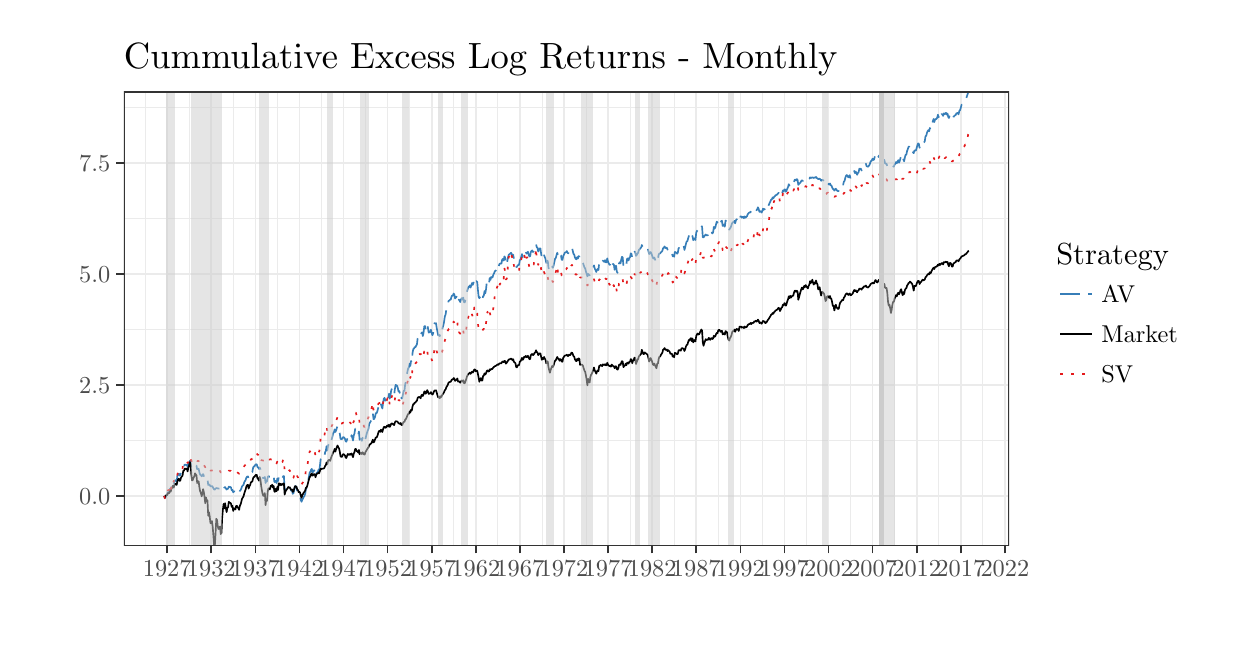
\begin{tikzpicture}[x=1pt,y=1pt]
\definecolor{fillColor}{RGB}{255,255,255}
\path[use as bounding box,fill=fillColor,fill opacity=0.00] (0,0) rectangle (426.79,216.81);
\begin{scope}
\path[clip] (  0.00,  0.00) rectangle (426.79,216.81);
\definecolor{drawColor}{RGB}{255,255,255}
\definecolor{fillColor}{RGB}{255,255,255}

\path[draw=drawColor,line width= 0.6pt,line join=round,line cap=round,fill=fillColor] (  0.00,  0.00) rectangle (426.79,216.81);
\end{scope}
\begin{scope}
\path[clip] ( 34.77, 29.59) rectangle (354.63,193.67);
\definecolor{fillColor}{RGB}{255,255,255}

\path[fill=fillColor] ( 34.77, 29.59) rectangle (354.63,193.67);
\definecolor{drawColor}{gray}{0.92}

\path[draw=drawColor,line width= 0.3pt,line join=round] ( 34.77, 67.61) --
	(354.63, 67.61);

\path[draw=drawColor,line width= 0.3pt,line join=round] ( 34.77,107.75) --
	(354.63,107.75);

\path[draw=drawColor,line width= 0.3pt,line join=round] ( 34.77,147.89) --
	(354.63,147.89);

\path[draw=drawColor,line width= 0.3pt,line join=round] ( 34.77,188.02) --
	(354.63,188.02);

\path[draw=drawColor,line width= 0.3pt,line join=round] ( 42.44, 29.59) --
	( 42.44,193.67);

\path[draw=drawColor,line width= 0.3pt,line join=round] ( 58.37, 29.59) --
	( 58.37,193.67);

\path[draw=drawColor,line width= 0.3pt,line join=round] ( 74.31, 29.59) --
	( 74.31,193.67);

\path[draw=drawColor,line width= 0.3pt,line join=round] ( 90.24, 29.59) --
	( 90.24,193.67);

\path[draw=drawColor,line width= 0.3pt,line join=round] (106.17, 29.59) --
	(106.17,193.67);

\path[draw=drawColor,line width= 0.3pt,line join=round] (122.10, 29.59) --
	(122.10,193.67);

\path[draw=drawColor,line width= 0.3pt,line join=round] (138.04, 29.59) --
	(138.04,193.67);

\path[draw=drawColor,line width= 0.3pt,line join=round] (153.97, 29.59) --
	(153.97,193.67);

\path[draw=drawColor,line width= 0.3pt,line join=round] (169.90, 29.59) --
	(169.90,193.67);

\path[draw=drawColor,line width= 0.3pt,line join=round] (185.83, 29.59) --
	(185.83,193.67);

\path[draw=drawColor,line width= 0.3pt,line join=round] (201.77, 29.59) --
	(201.77,193.67);

\path[draw=drawColor,line width= 0.3pt,line join=round] (217.70, 29.59) --
	(217.70,193.67);

\path[draw=drawColor,line width= 0.3pt,line join=round] (233.63, 29.59) --
	(233.63,193.67);

\path[draw=drawColor,line width= 0.3pt,line join=round] (249.57, 29.59) --
	(249.57,193.67);

\path[draw=drawColor,line width= 0.3pt,line join=round] (265.50, 29.59) --
	(265.50,193.67);

\path[draw=drawColor,line width= 0.3pt,line join=round] (281.44, 29.59) --
	(281.44,193.67);

\path[draw=drawColor,line width= 0.3pt,line join=round] (297.37, 29.59) --
	(297.37,193.67);

\path[draw=drawColor,line width= 0.3pt,line join=round] (313.30, 29.59) --
	(313.30,193.67);

\path[draw=drawColor,line width= 0.3pt,line join=round] (329.23, 29.59) --
	(329.23,193.67);

\path[draw=drawColor,line width= 0.3pt,line join=round] (345.17, 29.59) --
	(345.17,193.67);

\path[draw=drawColor,line width= 0.6pt,line join=round] ( 34.77, 47.54) --
	(354.63, 47.54);

\path[draw=drawColor,line width= 0.6pt,line join=round] ( 34.77, 87.68) --
	(354.63, 87.68);

\path[draw=drawColor,line width= 0.6pt,line join=round] ( 34.77,127.82) --
	(354.63,127.82);

\path[draw=drawColor,line width= 0.6pt,line join=round] ( 34.77,167.95) --
	(354.63,167.95);

\path[draw=drawColor,line width= 0.6pt,line join=round] ( 50.41, 29.59) --
	( 50.41,193.67);

\path[draw=drawColor,line width= 0.6pt,line join=round] ( 66.34, 29.59) --
	( 66.34,193.67);

\path[draw=drawColor,line width= 0.6pt,line join=round] ( 82.28, 29.59) --
	( 82.28,193.67);

\path[draw=drawColor,line width= 0.6pt,line join=round] ( 98.21, 29.59) --
	( 98.21,193.67);

\path[draw=drawColor,line width= 0.6pt,line join=round] (114.14, 29.59) --
	(114.14,193.67);

\path[draw=drawColor,line width= 0.6pt,line join=round] (130.07, 29.59) --
	(130.07,193.67);

\path[draw=drawColor,line width= 0.6pt,line join=round] (146.01, 29.59) --
	(146.01,193.67);

\path[draw=drawColor,line width= 0.6pt,line join=round] (161.94, 29.59) --
	(161.94,193.67);

\path[draw=drawColor,line width= 0.6pt,line join=round] (177.87, 29.59) --
	(177.87,193.67);

\path[draw=drawColor,line width= 0.6pt,line join=round] (193.80, 29.59) --
	(193.80,193.67);

\path[draw=drawColor,line width= 0.6pt,line join=round] (209.74, 29.59) --
	(209.74,193.67);

\path[draw=drawColor,line width= 0.6pt,line join=round] (225.67, 29.59) --
	(225.67,193.67);

\path[draw=drawColor,line width= 0.6pt,line join=round] (241.60, 29.59) --
	(241.60,193.67);

\path[draw=drawColor,line width= 0.6pt,line join=round] (257.53, 29.59) --
	(257.53,193.67);

\path[draw=drawColor,line width= 0.6pt,line join=round] (273.47, 29.59) --
	(273.47,193.67);

\path[draw=drawColor,line width= 0.6pt,line join=round] (289.40, 29.59) --
	(289.40,193.67);

\path[draw=drawColor,line width= 0.6pt,line join=round] (305.33, 29.59) --
	(305.33,193.67);

\path[draw=drawColor,line width= 0.6pt,line join=round] (321.26, 29.59) --
	(321.26,193.67);

\path[draw=drawColor,line width= 0.6pt,line join=round] (337.20, 29.59) --
	(337.20,193.67);

\path[draw=drawColor,line width= 0.6pt,line join=round] (353.13, 29.59) --
	(353.13,193.67);
\definecolor{drawColor}{RGB}{55,126,184}

\path[draw=drawColor,line width= 0.6pt,dash pattern=on 7pt off 3pt ,line join=round] ( 49.31, 47.61) --
	( 49.58, 46.82) --
	( 49.84, 47.22) --
	( 50.11, 47.85) --
	( 50.37, 47.83) --
	( 50.64, 48.93) --
	( 50.91, 48.96) --
	( 51.16, 49.05) --
	( 51.43, 50.24) --
	( 51.69, 49.70) --
	( 51.96, 51.16) --
	( 52.22, 51.62) --
	( 52.49, 52.47) --
	( 52.76, 51.59) --
	( 53.02, 52.85) --
	( 53.29, 53.30) --
	( 53.56, 53.18) --
	( 53.83, 52.79) --
	( 54.10, 54.88) --
	( 54.35, 55.42) --
	( 54.62, 55.62) --
	( 54.88, 55.00) --
	( 55.15, 55.05) --
	( 55.41, 56.24) --
	( 55.68, 56.69) --
	( 55.95, 56.95) --
	( 56.22, 58.52) --
	( 56.49, 58.53) --
	( 56.75, 58.89) --
	( 57.02, 58.88) --
	( 57.29, 58.74) --
	( 57.53, 58.87) --
	( 57.80, 58.09) --
	( 58.07, 58.97) --
	( 58.34, 59.42) --
	( 58.60, 60.28) --
	( 58.87, 59.80) --
	( 59.14, 57.72) --
	( 59.40, 57.59) --
	( 59.67, 57.61) --
	( 59.93, 57.83) --
	( 60.20, 58.08) --
	( 60.47, 58.99) --
	( 60.72, 58.73) --
	( 60.99, 58.52) --
	( 61.25, 57.25) --
	( 61.52, 57.41) --
	( 61.78, 57.42) --
	( 62.05, 56.09) --
	( 62.32, 55.27) --
	( 62.59, 55.15) --
	( 62.86, 54.71) --
	( 63.12, 54.98) --
	( 63.39, 55.50) --
	( 63.66, 54.82) --
	( 63.90, 54.13) --
	( 64.17, 53.56) --
	( 64.43, 54.02) --
	( 64.71, 53.84) --
	( 64.97, 53.86) --
	( 65.24, 51.55) --
	( 65.51, 51.74) --
	( 65.77, 51.62) --
	( 66.04, 51.07) --
	( 66.30, 51.05) --
	( 66.57, 51.17) --
	( 66.84, 50.91) --
	( 67.10, 50.40) --
	( 67.37, 49.92) --
	( 67.63, 49.91) --
	( 67.90, 50.28) --
	( 68.16, 50.45) --
	( 68.43, 50.41) --
	( 68.70, 50.30) --
	( 68.96, 50.23) --
	( 69.23, 50.34) --
	( 69.49, 50.36) --
	( 69.77, 49.49) --
	( 70.04, 49.61) --
	( 70.28, 50.13) --
	( 70.55, 50.50) --
	( 70.81, 50.85) --
	( 71.08, 50.60) --
	( 71.34, 50.80) --
	( 71.61, 50.28) --
	( 71.89, 49.92) --
	( 72.15, 50.15) --
	( 72.42, 50.24) --
	( 72.68, 50.96) --
	( 72.95, 50.81) --
	( 73.22, 50.84) --
	( 73.46, 50.69) --
	( 73.73, 49.63) --
	( 74.00, 49.80) --
	( 74.27, 48.93) --
	( 74.53, 49.21) --
	( 74.80, 49.20) --
	( 75.07, 49.04) --
	( 75.33, 49.68) --
	( 75.60, 49.71) --
	( 75.86, 49.39) --
	( 76.13, 49.14) --
	( 76.40, 48.71) --
	( 76.65, 49.37) --
	( 76.92, 49.70) --
	( 77.18, 50.21) --
	( 77.45, 51.01) --
	( 77.71, 51.36) --
	( 77.98, 51.58) --
	( 78.25, 52.52) --
	( 78.52, 52.96) --
	( 78.79, 53.46) --
	( 79.05, 54.26) --
	( 79.32, 54.56) --
	( 79.59, 54.67) --
	( 79.84, 53.85) --
	( 80.11, 54.34) --
	( 80.37, 54.65) --
	( 80.64, 55.89) --
	( 80.91, 56.08) --
	( 81.18, 56.28) --
	( 81.45, 57.75) --
	( 81.71, 58.28) --
	( 81.98, 58.31) --
	( 82.24, 58.84) --
	( 82.51, 59.05) --
	( 82.78, 59.00) --
	( 83.03, 58.02) --
	( 83.30, 57.95) --
	( 83.56, 57.38) --
	( 83.83, 57.85) --
	( 84.09, 57.29) --
	( 84.36, 54.72) --
	( 84.63, 54.33) --
	( 84.89, 54.18) --
	( 85.16, 54.07) --
	( 85.43, 54.12) --
	( 85.70, 54.46) --
	( 85.97, 52.29) --
	( 86.21, 52.98) --
	( 86.48, 52.83) --
	( 86.74, 54.36) --
	( 87.01, 54.76) --
	( 87.28, 54.55) --
	( 87.55, 54.58) --
	( 87.82, 54.88) --
	( 88.08, 54.71) --
	( 88.35, 55.18) --
	( 88.61, 54.50) --
	( 88.88, 54.77) --
	( 89.15, 52.65) --
	( 89.40, 52.63) --
	( 89.67, 53.05) --
	( 89.93, 52.27) --
	( 90.20, 53.89) --
	( 90.46, 52.98) --
	( 90.73, 54.29) --
	( 91.00, 54.27) --
	( 91.26, 53.56) --
	( 91.53, 54.28) --
	( 91.79, 53.74) --
	( 92.06, 54.09) --
	( 92.34, 54.76) --
	( 92.59, 54.78) --
	( 92.86, 49.55) --
	( 93.12, 49.76) --
	( 93.39, 49.94) --
	( 93.65, 50.40) --
	( 93.92, 50.70) --
	( 94.19, 51.10) --
	( 94.46, 50.78) --
	( 94.73, 50.84) --
	( 94.99, 49.74) --
	( 95.26, 49.45) --
	( 95.53, 49.62) --
	( 95.77, 48.37) --
	( 96.04, 48.60) --
	( 96.30, 49.72) --
	( 96.58, 51.12) --
	( 96.84, 51.09) --
	( 97.11, 50.84) --
	( 97.38, 49.41) --
	( 97.64, 48.95) --
	( 97.91, 47.86) --
	( 98.17, 47.92) --
	( 98.44, 47.61) --
	( 98.71, 46.10) --
	( 98.96, 45.49) --
	( 99.23, 46.26) --
	( 99.49, 46.66) --
	( 99.76, 47.29) --
	(100.02, 47.63) --
	(100.29, 48.39) --
	(100.56, 50.36) --
	(100.82, 50.37) --
	(101.09, 51.59) --
	(101.36, 53.07) --
	(101.63, 54.54) --
	(101.90, 56.12) --
	(102.14, 56.25) --
	(102.41, 57.06) --
	(102.67, 57.38) --
	(102.94, 56.15) --
	(103.21, 56.38) --
	(103.48, 56.88) --
	(103.75, 56.48) --
	(104.01, 54.54) --
	(104.28, 55.63) --
	(104.54, 56.03) --
	(104.81, 56.14) --
	(105.08, 57.05) --
	(105.33, 56.52) --
	(105.60, 58.48) --
	(105.87, 60.85) --
	(106.14, 60.42) --
	(106.40, 60.84) --
	(106.67, 60.85) --
	(106.94, 60.90) --
	(107.20, 61.62) --
	(107.47, 63.33) --
	(107.73, 63.89) --
	(108.00, 65.58) --
	(108.27, 64.04) --
	(108.52, 65.75) --
	(108.79, 66.26) --
	(109.05, 66.38) --
	(109.32, 65.82) --
	(109.58, 67.14) --
	(109.85, 68.06) --
	(110.12, 69.05) --
	(110.39, 70.30) --
	(110.66, 70.54) --
	(110.92, 71.62) --
	(111.19, 70.71) --
	(111.46, 71.32) --
	(111.70, 72.09) --
	(111.97, 72.94) --
	(112.24, 72.12) --
	(112.51, 71.54) --
	(112.77, 70.26) --
	(113.04, 68.22) --
	(113.31, 68.16) --
	(113.57, 68.16) --
	(113.84, 68.72) --
	(114.10, 68.86) --
	(114.37, 68.67) --
	(114.64, 68.26) --
	(114.89, 67.37) --
	(115.16, 67.19) --
	(115.42, 68.04) --
	(115.69, 68.86) --
	(115.95, 68.51) --
	(116.22, 68.37) --
	(116.49, 68.99) --
	(116.75, 68.47) --
	(117.03, 69.56) --
	(117.29, 68.68) --
	(117.56, 67.64) --
	(117.83, 69.45) --
	(118.08, 70.14) --
	(118.35, 71.88) --
	(118.61, 71.86) --
	(118.88, 70.54) --
	(119.15, 70.60) --
	(119.42, 69.67) --
	(119.69, 70.88) --
	(119.95, 67.88) --
	(120.22, 68.24) --
	(120.48, 68.31) --
	(120.75, 67.52) --
	(121.02, 68.61) --
	(121.27, 68.08) --
	(121.54, 66.92) --
	(121.80, 66.96) --
	(122.07, 68.24) --
	(122.33, 69.40) --
	(122.60, 70.41) --
	(122.87, 71.19) --
	(123.13, 71.83) --
	(123.40, 73.55) --
	(123.66, 74.07) --
	(123.93, 74.50) --
	(124.21, 75.03) --
	(124.45, 76.32) --
	(124.72, 77.55) --
	(124.98, 75.32) --
	(125.25, 75.49) --
	(125.51, 76.14) --
	(125.78, 77.49) --
	(126.05, 77.42) --
	(126.32, 78.09) --
	(126.59, 79.12) --
	(126.85, 80.02) --
	(127.12, 80.29) --
	(127.39, 79.45) --
	(127.63, 80.78) --
	(127.90, 79.97) --
	(128.17, 79.21) --
	(128.44, 81.48) --
	(128.70, 82.75) --
	(128.97, 83.03) --
	(129.24, 82.03) --
	(129.50, 82.14) --
	(129.77, 83.23) --
	(130.03, 83.94) --
	(130.30, 82.95) --
	(130.57, 84.51) --
	(130.83, 82.74) --
	(131.10, 83.94) --
	(131.36, 85.76) --
	(131.63, 86.38) --
	(131.89, 85.92) --
	(132.16, 84.50) --
	(132.43, 84.15) --
	(132.69, 86.28) --
	(132.96, 87.72) --
	(133.23, 87.58) --
	(133.50, 87.40) --
	(133.77, 86.53) --
	(134.01, 85.34) --
	(134.28, 85.51) --
	(134.54, 84.53) --
	(134.81, 85.32) --
	(135.08, 82.82) --
	(135.35, 82.90) --
	(135.62, 84.38) --
	(135.88, 85.66) --
	(136.15, 85.62) --
	(136.41, 87.98) --
	(136.68, 88.77) --
	(136.95, 90.64) --
	(137.20, 92.43) --
	(137.47, 93.63) --
	(137.73, 94.10) --
	(138.00, 95.41) --
	(138.26, 94.56) --
	(138.53, 96.38) --
	(138.80, 95.66) --
	(139.06, 99.20) --
	(139.33,100.66) --
	(139.60,100.84) --
	(139.87,101.41) --
	(140.14,101.34) --
	(140.38,101.92) --
	(140.65,102.33) --
	(140.91,104.48) --
	(141.18,105.12) --
	(141.44,105.19) --
	(141.72,105.09) --
	(141.99,104.76) --
	(142.25,106.36) --
	(142.52,106.71) --
	(142.78,105.37) --
	(143.05,106.61) --
	(143.32,108.90) --
	(143.57,109.00) --
	(143.84,107.55) --
	(144.11,108.36) --
	(144.38,109.51) --
	(144.64,108.29) --
	(144.91,106.60) --
	(145.18,106.82) --
	(145.44,106.90) --
	(145.71,107.69) --
	(145.97,106.48) --
	(146.24,105.69) --
	(146.51,106.36) --
	(146.76,108.65) --
	(147.03,110.06) --
	(147.29,109.80) --
	(147.56,110.02) --
	(147.82,108.19) --
	(148.09,106.84) --
	(148.36,105.63) --
	(148.62,105.86) --
	(148.90,105.34) --
	(149.16,106.50) --
	(149.43,106.04) --
	(149.70,107.23) --
	(149.94,108.43) --
	(150.21,109.29) --
	(150.47,110.57) --
	(150.74,112.51) --
	(151.01,113.13) --
	(151.28,115.01) --
	(151.55,116.03) --
	(151.81,116.80) --
	(152.08,118.04) --
	(152.34,118.22) --
	(152.61,118.49) --
	(152.88,118.57) --
	(153.13,119.56) --
	(153.40,120.03) --
	(153.66,119.99) --
	(153.93,120.73) --
	(154.19,120.33) --
	(154.46,118.96) --
	(154.73,119.26) --
	(154.99,119.67) --
	(155.26,120.36) --
	(155.53,118.20) --
	(155.80,118.55) --
	(156.07,118.14) --
	(156.32,117.68) --
	(156.59,118.58) --
	(156.85,119.07) --
	(157.12,118.54) --
	(157.38,119.27) --
	(157.65,117.65) --
	(157.92,117.51) --
	(158.19,118.54) --
	(158.46,119.87) --
	(158.72,121.42) --
	(158.99,122.27) --
	(159.26,123.10) --
	(159.50,123.20) --
	(159.77,123.67) --
	(160.04,122.87) --
	(160.31,123.75) --
	(160.57,124.54) --
	(160.84,123.89) --
	(161.11,124.65) --
	(161.37,125.95) --
	(161.64,125.92) --
	(161.90,124.75) --
	(162.17,125.21) --
	(162.44,124.92) --
	(162.69,122.08) --
	(162.96,119.51) --
	(163.22,119.06) --
	(163.49,119.57) --
	(163.75,119.96) --
	(164.02,118.43) --
	(164.29,118.43) --
	(164.56,119.74) --
	(164.83,119.98) --
	(165.09,121.63) --
	(165.36,120.81) --
	(165.63,122.33) --
	(165.87,124.63) --
	(166.14,125.34) --
	(166.40,124.42) --
	(166.68,124.21) --
	(166.94,126.34) --
	(167.21,125.66) --
	(167.48,126.71) --
	(167.74,126.47) --
	(168.01,126.71) --
	(168.27,127.59) --
	(168.54,128.06) --
	(168.81,128.82) --
	(169.07,128.91) --
	(169.34,129.44) --
	(169.60,129.96) --
	(169.87,130.66) --
	(170.13,129.98) --
	(170.40,131.26) --
	(170.67,131.56) --
	(170.93,131.57) --
	(171.20,131.61) --
	(171.47,133.04) --
	(171.74,133.24) --
	(172.01,132.66) --
	(172.25,134.17) --
	(172.52,133.76) --
	(172.78,131.04) --
	(173.05,131.35) --
	(173.31,132.45) --
	(173.59,133.87) --
	(173.86,134.84) --
	(174.12,134.84) --
	(174.39,135.22) --
	(174.65,135.45) --
	(174.92,135.07) --
	(175.19,134.28) --
	(175.43,134.74) --
	(175.71,133.22) --
	(175.97,133.01) --
	(176.24,132.59) --
	(176.50,130.41) --
	(176.77,130.29) --
	(177.04,130.88) --
	(177.30,131.04) --
	(177.57,131.08) --
	(177.83,132.84) --
	(178.10,132.99) --
	(178.37,134.11) --
	(178.62,134.98) --
	(178.89,133.89) --
	(179.15,134.44) --
	(179.42,135.35) --
	(179.68,135.15) --
	(179.95,136.00) --
	(180.22,135.18) --
	(180.49,135.29) --
	(180.76,135.85) --
	(181.02,134.85) --
	(181.29,134.14) --
	(181.56,134.17) --
	(181.81,135.77) --
	(182.08,136.14) --
	(182.34,136.30) --
	(182.61,135.74) --
	(182.88,136.02) --
	(183.15,137.13) --
	(183.42,137.26) --
	(183.68,138.63) --
	(183.95,137.52) --
	(184.21,137.25) --
	(184.48,135.93) --
	(184.75,136.64) --
	(185.00,137.05) --
	(185.27,137.06) --
	(185.53,135.14) --
	(185.80,133.51) --
	(186.06,134.14) --
	(186.33,133.59) --
	(186.60,134.57) --
	(186.86,133.90) --
	(187.13,133.22) --
	(187.40,131.81) --
	(187.67,132.62) --
	(187.94,132.45) --
	(188.18,130.14) --
	(188.45,128.96) --
	(188.71,128.63) --
	(188.98,129.33) --
	(189.25,129.86) --
	(189.52,130.44) --
	(189.79,130.04) --
	(190.05,130.89) --
	(190.32,132.17) --
	(190.58,133.33) --
	(190.85,133.62) --
	(191.12,134.70) --
	(191.37,135.47) --
	(191.64,134.49) --
	(191.90,134.50) --
	(192.17,133.49) --
	(192.43,134.62) --
	(192.70,134.49) --
	(192.97,132.99) --
	(193.23,132.86) --
	(193.50,134.26) --
	(193.76,134.73) --
	(194.03,135.43) --
	(194.31,135.60) --
	(194.56,135.67) --
	(194.83,136.09) --
	(195.09,135.48) --
	(195.36,135.26) --
	(195.62,136.06) --
	(195.89,135.84) --
	(196.16,136.02) --
	(196.43,137.09) --
	(196.70,137.26) --
	(196.96,136.20) --
	(197.23,135.05) --
	(197.50,134.82) --
	(197.74,133.79) --
	(198.01,133.28) --
	(198.27,133.12) --
	(198.55,133.88) --
	(198.81,133.38) --
	(199.08,134.25) --
	(199.35,134.13) --
	(199.61,132.21) --
	(199.88,132.25) --
	(200.14,132.25) --
	(200.41,132.21) --
	(200.68,131.76) --
	(200.93,130.92) --
	(201.20,130.15) --
	(201.46,129.79) --
	(201.73,128.67) --
	(201.99,127.90) --
	(202.26,126.93) --
	(202.53,127.81) --
	(202.79,127.59) --
	(203.06,127.31) --
	(203.33,128.46) --
	(203.60,128.84) --
	(203.87,129.12) --
	(204.11,129.64) --
	(204.38,130.25) --
	(204.64,130.90) --
	(204.91,129.74) --
	(205.18,129.20) --
	(205.45,128.54) --
	(205.72,129.27) --
	(205.98,129.65) --
	(206.25,129.24) --
	(206.51,131.67) --
	(206.78,131.71) --
	(207.05,132.14) --
	(207.30,131.87) --
	(207.58,131.54) --
	(207.84,132.62) --
	(208.11,132.37) --
	(208.37,132.18) --
	(208.64,132.79) --
	(208.91,132.00) --
	(209.17,132.03) --
	(209.44,133.45) --
	(209.70,132.24) --
	(209.97,131.63) --
	(210.24,131.13) --
	(210.49,131.18) --
	(210.76,130.75) --
	(211.02,132.52) --
	(211.29,131.89) --
	(211.55,131.30) --
	(211.82,131.21) --
	(212.09,129.32) --
	(212.36,130.63) --
	(212.63,130.72) --
	(212.89,128.64) --
	(213.16,128.20) --
	(213.43,129.31) --
	(213.67,131.61) --
	(213.94,132.02) --
	(214.21,131.64) --
	(214.48,132.97) --
	(214.74,134.01) --
	(215.01,133.75) --
	(215.28,130.67) --
	(215.54,131.17) --
	(215.81,131.33) --
	(216.07,132.25) --
	(216.34,131.39) --
	(216.61,133.35) --
	(216.86,133.39) --
	(217.13,132.70) --
	(217.39,133.63) --
	(217.66,133.81) --
	(217.92,135.24) --
	(218.19,135.07) --
	(218.46,133.48) --
	(218.72,134.18) --
	(219.00,134.53) --
	(219.26,135.85) --
	(219.53,135.76) --
	(219.80,134.34) --
	(220.05,134.63) --
	(220.32,135.11) --
	(220.58,135.48) --
	(220.85,136.47) --
	(221.12,136.75) --
	(221.39,137.14) --
	(221.66,137.29) --
	(221.92,138.27) --
	(222.19,137.71) --
	(222.45,137.21) --
	(222.72,137.24) --
	(222.99,137.78) --
	(223.24,137.54) --
	(223.51,137.56) --
	(223.77,137.25) --
	(224.04,137.09) --
	(224.30,136.06) --
	(224.57,134.99) --
	(224.84,135.42) --
	(225.10,135.72) --
	(225.37,135.25) --
	(225.63,134.49) --
	(225.90,133.69) --
	(226.18,133.39) --
	(226.42,133.75) --
	(226.69,133.11) --
	(226.95,132.31) --
	(227.22,131.87) --
	(227.48,133.38) --
	(227.75,133.42) --
	(228.02,134.88) --
	(228.29,135.18) --
	(228.56,135.26) --
	(228.82,135.62) --
	(229.09,135.84) --
	(229.36,136.24) --
	(229.60,137.13) --
	(229.87,137.25) --
	(230.14,137.75) --
	(230.41,137.23) --
	(230.67,137.18) --
	(230.94,137.31) --
	(231.21,136.62) --
	(231.47,136.97) --
	(231.74,136.62) --
	(232.00,136.19) --
	(232.27,135.37) --
	(232.54,135.44) --
	(232.80,135.37) --
	(233.07,134.20) --
	(233.33,134.48) --
	(233.60,134.02) --
	(233.86,135.75) --
	(234.13,135.66) --
	(234.40,135.47) --
	(234.66,135.13) --
	(234.93,135.48) --
	(235.20,137.09) --
	(235.47,137.28) --
	(235.74,137.08) --
	(235.98,136.91) --
	(236.25,138.19) --
	(236.51,138.41) --
	(236.78,138.23) --
	(237.05,138.00) --
	(237.32,136.49) --
	(237.59,137.49) --
	(237.85,138.63) --
	(238.12,139.59) --
	(238.38,139.66) --
	(238.65,140.65) --
	(238.92,141.54) --
	(239.17,141.32) --
	(239.44,141.91) --
	(239.70,142.08) --
	(239.97,140.79) --
	(240.23,141.55) --
	(240.50,140.00) --
	(240.77,140.48) --
	(241.03,140.67) --
	(241.30,140.09) --
	(241.57,142.71) --
	(241.84,143.33) --
	(242.11,143.67) --
	(242.35,143.33) --
	(242.62,143.34) --
	(242.88,143.84) --
	(243.15,144.66) --
	(243.41,145.30) --
	(243.69,144.86) --
	(243.96,141.10) --
	(244.22,141.01) --
	(244.49,141.46) --
	(244.75,141.76) --
	(245.02,142.07) --
	(245.29,141.74) --
	(245.54,141.84) --
	(245.81,141.78) --
	(246.08,142.64) --
	(246.35,142.41) --
	(246.61,141.64) --
	(246.88,142.44) --
	(247.15,142.75) --
	(247.41,142.45) --
	(247.68,142.84) --
	(247.94,144.82) --
	(248.21,144.20) --
	(248.48,144.66) --
	(248.73,145.69) --
	(249.00,146.72) --
	(249.26,146.40) --
	(249.53,147.64) --
	(249.79,148.02) --
	(250.06,147.84) --
	(250.33,146.66) --
	(250.59,146.77) --
	(250.87,147.06) --
	(251.13,145.15) --
	(251.40,145.28) --
	(251.67,145.73) --
	(251.91,144.89) --
	(252.18,147.13) --
	(252.44,146.86) --
	(252.71,146.48) --
	(252.98,144.61) --
	(253.25,144.11) --
	(253.52,143.84) --
	(253.78,144.32) --
	(254.05,144.63) --
	(254.31,145.45) --
	(254.58,146.22) --
	(254.85,146.52) --
	(255.10,146.49) --
	(255.37,147.01) --
	(255.63,146.11) --
	(255.90,147.12) --
	(256.16,147.59) --
	(256.43,147.31) --
	(256.70,147.66) --
	(256.96,146.92) --
	(257.23,148.61) --
	(257.50,148.53) --
	(257.77,148.65) --
	(258.04,148.15) --
	(258.29,148.42) --
	(258.56,148.47) --
	(258.82,147.94) --
	(259.09,148.63) --
	(259.35,148.14) --
	(259.62,148.42) --
	(259.89,148.61) --
	(260.16,149.33) --
	(260.43,149.70) --
	(260.69,149.94) --
	(260.96,149.99) --
	(261.23,150.32) --
	(261.47,149.81) --
	(261.74,150.14) --
	(262.01,150.20) --
	(262.28,150.14) --
	(262.54,150.91) --
	(262.81,150.87) --
	(263.08,151.19) --
	(263.34,150.84) --
	(263.61,151.15) --
	(263.87,151.89) --
	(264.14,151.34) --
	(264.41,150.27) --
	(264.66,150.40) --
	(264.93,150.49) --
	(265.19,149.98) --
	(265.46,150.52) --
	(265.72,151.44) --
	(265.99,151.00) --
	(266.26,151.28) --
	(266.53,150.39) --
	(266.80,150.58) --
	(267.06,150.95) --
	(267.33,151.75) --
	(267.60,152.39) --
	(267.84,152.86) --
	(268.11,153.51) --
	(268.38,154.01) --
	(268.65,154.69) --
	(268.91,154.76) --
	(269.18,155.47) --
	(269.45,155.13) --
	(269.71,155.68) --
	(269.98,155.85) --
	(270.24,156.24) --
	(270.51,156.37) --
	(270.78,156.48) --
	(271.04,156.76) --
	(271.31,157.12) --
	(271.57,156.88) --
	(271.84,155.55) --
	(272.10,155.86) --
	(272.37,156.75) --
	(272.64,156.95) --
	(272.90,157.98) --
	(273.17,157.67) --
	(273.44,158.39) --
	(273.71,158.31) --
	(273.98,157.52) --
	(274.22,158.00) --
	(274.49,158.64) --
	(274.75,159.21) --
	(275.02,160.24) --
	(275.28,159.76) --
	(275.56,160.49) --
	(275.83,159.96) --
	(276.09,160.11) --
	(276.36,160.29) --
	(276.62,160.30) --
	(276.89,161.01) --
	(277.16,161.83) --
	(277.40,161.93) --
	(277.68,161.62) --
	(277.94,162.08) --
	(278.21,161.75) --
	(278.47,160.00) --
	(278.74,160.34) --
	(279.01,160.63) --
	(279.27,160.86) --
	(279.54,161.43) --
	(279.80,161.69) --
	(280.07,161.43) --
	(280.34,161.69) --
	(280.59,162.01) --
	(280.86,161.90) --
	(281.12,162.22) --
	(281.39,161.97) --
	(281.65,161.83) --
	(281.92,161.61) --
	(282.19,162.07) --
	(282.46,162.24) --
	(282.73,162.70) --
	(282.99,162.49) --
	(283.26,162.57) --
	(283.53,162.76) --
	(283.78,162.59) --
	(284.05,162.50) --
	(284.31,162.67) --
	(284.58,162.57) --
	(284.85,162.87) --
	(285.12,162.51) --
	(285.39,162.36) --
	(285.65,162.10) --
	(285.92,162.15) --
	(286.18,162.25) --
	(286.45,161.98) --
	(286.72,161.49) --
	(286.97,161.78) --
	(287.24,161.80) --
	(287.50,161.62) --
	(287.77,161.41) --
	(288.03,160.93) --
	(288.30,159.80) --
	(288.57,159.93) --
	(288.83,160.36) --
	(289.10,160.53) --
	(289.37,160.32) --
	(289.64,160.08) --
	(289.91,160.52) --
	(290.15,159.89) --
	(290.42,159.77) --
	(290.68,159.17) --
	(290.95,158.48) --
	(291.22,158.50) --
	(291.49,157.92) --
	(291.76,158.40) --
	(292.02,158.61) --
	(292.29,158.19) --
	(292.55,157.86) --
	(292.82,157.71) --
	(293.09,157.86) --
	(293.34,158.58) --
	(293.61,159.38) --
	(293.87,159.60) --
	(294.14,159.96) --
	(294.40,160.33) --
	(294.67,160.08) --
	(294.94,161.19) --
	(295.20,161.48) --
	(295.47,162.65) --
	(295.73,163.28) --
	(296.00,163.55) --
	(296.28,163.24) --
	(296.53,162.72) --
	(296.80,162.97) --
	(297.06,163.49) --
	(297.33,162.29) --
	(297.59,162.33) --
	(297.86,162.80) --
	(298.13,163.24) --
	(298.40,164.15) --
	(298.67,165.04) --
	(298.93,164.24) --
	(299.20,164.80) --
	(299.47,164.29) --
	(299.71,163.63) --
	(299.98,164.28) --
	(300.25,164.56) --
	(300.52,165.86) --
	(300.78,165.63) --
	(301.05,165.87) --
	(301.32,165.21) --
	(301.58,165.78) --
	(301.85,165.80) --
	(302.11,167.02) --
	(302.38,166.92) --
	(302.65,167.34) --
	(302.90,167.60) --
	(303.17,166.72) --
	(303.43,166.65) --
	(303.70,166.55) --
	(303.96,166.91) --
	(304.23,167.30) --
	(304.50,168.17) --
	(304.76,168.64) --
	(305.03,168.82) --
	(305.30,169.47) --
	(305.57,168.99) --
	(305.84,169.22) --
	(306.08,170.14) --
	(306.35,171.21) --
	(306.61,170.66) --
	(306.88,169.70) --
	(307.15,169.83) --
	(307.42,170.16) --
	(307.69,170.64) --
	(307.95,169.90) --
	(308.22,169.84) --
	(308.48,168.79) --
	(308.75,168.62) --
	(309.02,168.49) --
	(309.27,168.80) --
	(309.55,169.01) --
	(309.81,167.81) --
	(310.08,167.64) --
	(310.34,167.68) --
	(310.61,166.76) --
	(310.88,166.32) --
	(311.14,166.23) --
	(311.41,166.26) --
	(311.67,166.04) --
	(311.94,165.70) --
	(312.21,166.08) --
	(312.46,166.33) --
	(312.73,166.60) --
	(312.99,166.58) --
	(313.26,167.35) --
	(313.52,167.65) --
	(313.79,168.25) --
	(314.06,167.82) --
	(314.33,168.40) --
	(314.60,168.93) --
	(314.86,168.03) --
	(315.13,168.63) --
	(315.40,169.77) --
	(315.64,170.39) --
	(315.91,168.90) --
	(316.18,168.47) --
	(316.45,169.18) --
	(316.71,168.53) --
	(316.98,170.00) --
	(317.25,170.84) --
	(317.51,170.95) --
	(317.78,172.29) --
	(318.04,172.93) --
	(318.31,173.79) --
	(318.58,173.87) --
	(318.83,174.39) --
	(319.10,173.95) --
	(319.36,173.45) --
	(319.63,173.00) --
	(319.89,171.81) --
	(320.16,171.46) --
	(320.43,172.43) --
	(320.69,172.38) --
	(320.97,172.42) --
	(321.23,173.34) --
	(321.50,174.29) --
	(321.77,174.99) --
	(322.02,174.81) --
	(322.29,173.41) --
	(322.55,174.20) --
	(322.82,174.36) --
	(323.09,174.86) --
	(323.36,175.73) --
	(323.63,175.27) --
	(323.89,175.43) --
	(324.16,175.71) --
	(324.42,177.56) --
	(324.69,177.77) --
	(324.96,178.79) --
	(325.21,179.43) --
	(325.48,179.78) --
	(325.74,179.39) --
	(326.01,180.55) --
	(326.27,179.91) --
	(326.54,180.99) --
	(326.81,182.34) --
	(327.07,182.91) --
	(327.34,183.82) --
	(327.60,182.69) --
	(327.88,183.65) --
	(328.15,183.78) --
	(328.39,183.83) --
	(328.66,184.27) --
	(328.92,185.35) --
	(329.19,184.42) --
	(329.45,185.59) --
	(329.72,184.49) --
	(330.00,185.29) --
	(330.26,185.60) --
	(330.53,185.47) --
	(330.79,184.92) --
	(331.06,185.85) --
	(331.33,185.56) --
	(331.57,185.75) --
	(331.84,186.04) --
	(332.11,185.37) --
	(332.38,185.79) --
	(332.64,184.55) --
	(332.91,184.17) --
	(333.18,185.18) --
	(333.44,185.22) --
	(333.71,184.71) --
	(333.97,183.75) --
	(334.24,183.75) --
	(334.51,184.55) --
	(334.77,184.82) --
	(335.04,185.13) --
	(335.30,185.21) --
	(335.57,185.82) --
	(335.83,185.91) --
	(336.10,186.03) --
	(336.37,185.46) --
	(336.63,186.69) --
	(336.90,186.99) --
	(337.17,187.80) --
	(337.44,188.93) --
	(337.71,189.00) --
	(337.95,189.39) --
	(338.22,189.85) --
	(338.48,190.17) --
	(338.75,190.84) --
	(339.02,190.88) --
	(339.29,191.72) --
	(339.56,192.54) --
	(339.82,193.33) --
	(340.09,193.67);
\definecolor{drawColor}{RGB}{0,0,0}

\path[draw=drawColor,line width= 0.6pt,line join=round] ( 49.31, 47.60) --
	( 49.58, 47.09) --
	( 49.84, 47.50) --
	( 50.11, 47.91) --
	( 50.37, 47.90) --
	( 50.64, 48.57) --
	( 50.91, 48.59) --
	( 51.16, 48.66) --
	( 51.43, 49.52) --
	( 51.69, 49.14) --
	( 51.96, 50.25) --
	( 52.22, 50.57) --
	( 52.49, 51.30) --
	( 52.76, 50.59) --
	( 53.02, 51.62) --
	( 53.29, 51.96) --
	( 53.56, 51.87) --
	( 53.83, 51.60) --
	( 54.10, 52.95) --
	( 54.35, 53.59) --
	( 54.62, 53.82) --
	( 54.88, 53.04) --
	( 55.15, 53.14) --
	( 55.41, 54.18) --
	( 55.68, 54.63) --
	( 55.95, 54.88) --
	( 56.22, 56.68) --
	( 56.49, 56.70) --
	( 56.75, 57.49) --
	( 57.02, 57.47) --
	( 57.29, 57.29) --
	( 57.53, 57.50) --
	( 57.80, 56.46) --
	( 58.07, 57.95) --
	( 58.34, 58.60) --
	( 58.60, 59.83) --
	( 58.87, 58.95) --
	( 59.14, 55.37) --
	( 59.40, 53.19) --
	( 59.67, 53.38) --
	( 59.93, 54.23) --
	( 60.20, 54.62) --
	( 60.47, 55.75) --
	( 60.72, 55.37) --
	( 60.99, 55.09) --
	( 61.25, 52.26) --
	( 61.52, 52.87) --
	( 61.78, 52.89) --
	( 62.05, 50.72) --
	( 62.32, 49.25) --
	( 62.59, 48.76) --
	( 62.86, 47.44) --
	( 63.12, 48.42) --
	( 63.39, 50.06) --
	( 63.66, 49.00) --
	( 63.90, 47.30) --
	( 64.17, 44.97) --
	( 64.43, 47.06) --
	( 64.71, 45.95) --
	( 64.97, 45.98) --
	( 65.24, 40.43) --
	( 65.51, 41.69) --
	( 65.77, 40.20) --
	( 66.04, 37.85) --
	( 66.30, 37.66) --
	( 66.57, 38.54) --
	( 66.84, 36.62) --
	( 67.10, 33.41) --
	( 67.37, 29.67) --
	( 67.63, 29.59) --
	( 67.90, 34.28) --
	( 68.16, 39.35) --
	( 68.43, 38.88) --
	( 68.70, 36.59) --
	( 68.96, 35.62) --
	( 69.23, 36.33) --
	( 69.49, 36.48) --
	( 69.77, 33.81) --
	( 70.04, 34.33) --
	( 70.28, 39.67) --
	( 70.55, 42.77) --
	( 70.81, 44.76) --
	( 71.08, 43.13) --
	( 71.34, 44.97) --
	( 71.61, 43.17) --
	( 71.89, 41.76) --
	( 72.15, 43.28) --
	( 72.42, 43.57) --
	( 72.68, 45.48) --
	( 72.95, 45.08) --
	( 73.22, 45.15) --
	( 73.46, 44.85) --
	( 73.73, 43.64) --
	( 74.00, 44.04) --
	( 74.27, 42.18) --
	( 74.53, 43.07) --
	( 74.80, 43.03) --
	( 75.07, 42.72) --
	( 75.33, 43.98) --
	( 75.60, 44.04) --
	( 75.86, 43.49) --
	( 76.13, 43.17) --
	( 76.40, 42.58) --
	( 76.65, 43.97) --
	( 76.92, 44.51) --
	( 77.18, 45.42) --
	( 77.45, 46.56) --
	( 77.71, 46.98) --
	( 77.98, 47.40) --
	( 78.25, 48.47) --
	( 78.52, 49.30) --
	( 78.79, 50.03) --
	( 79.05, 51.11) --
	( 79.32, 51.51) --
	( 79.59, 51.64) --
	( 79.84, 50.27) --
	( 80.11, 51.09) --
	( 80.37, 51.47) --
	( 80.64, 52.50) --
	( 80.91, 52.67) --
	( 81.18, 52.85) --
	( 81.45, 53.94) --
	( 81.71, 54.45) --
	( 81.98, 54.50) --
	( 82.24, 55.02) --
	( 82.51, 55.23) --
	( 82.78, 55.18) --
	( 83.03, 53.92) --
	( 83.30, 53.81) --
	( 83.56, 53.12) --
	( 83.83, 54.49) --
	( 84.09, 53.69) --
	( 84.36, 51.32) --
	( 84.63, 49.70) --
	( 84.89, 48.30) --
	( 85.16, 47.63) --
	( 85.43, 47.74) --
	( 85.70, 48.64) --
	( 85.97, 44.27) --
	( 86.21, 46.46) --
	( 86.48, 45.82) --
	( 86.74, 49.25) --
	( 87.01, 50.36) --
	( 87.28, 49.92) --
	( 87.55, 50.07) --
	( 87.82, 51.28) --
	( 88.08, 50.99) --
	( 88.35, 51.64) --
	( 88.61, 50.65) --
	( 88.88, 51.21) --
	( 89.15, 49.15) --
	( 89.40, 49.11) --
	( 89.67, 50.19) --
	( 89.93, 49.30) --
	( 90.20, 50.86) --
	( 90.46, 49.74) --
	( 90.73, 52.15) --
	( 91.00, 52.08) --
	( 91.26, 51.48) --
	( 91.53, 51.95) --
	( 91.79, 51.55) --
	( 92.06, 51.79) --
	( 92.34, 52.08) --
	( 92.59, 52.10) --
	( 92.86, 48.09) --
	( 93.12, 49.12) --
	( 93.39, 49.63) --
	( 93.65, 50.02) --
	( 93.92, 50.38) --
	( 94.19, 50.86) --
	( 94.46, 50.59) --
	( 94.73, 50.70) --
	( 94.99, 50.02) --
	( 95.26, 49.80) --
	( 95.53, 49.95) --
	( 95.77, 49.06) --
	( 96.04, 49.27) --
	( 96.30, 50.18) --
	( 96.58, 51.11) --
	( 96.84, 51.09) --
	( 97.11, 50.96) --
	( 97.38, 50.09) --
	( 97.64, 49.76) --
	( 97.91, 48.99) --
	( 98.17, 49.14) --
	( 98.44, 48.75) --
	( 98.71, 47.66) --
	( 98.96, 46.95) --
	( 99.23, 47.88) --
	( 99.49, 48.29) --
	( 99.76, 48.84) --
	(100.02, 49.13) --
	(100.29, 49.56) --
	(100.56, 50.63) --
	(100.82, 50.64) --
	(101.09, 51.44) --
	(101.36, 52.57) --
	(101.63, 53.51) --
	(101.90, 54.47) --
	(102.14, 54.58) --
	(102.41, 55.47) --
	(102.67, 55.74) --
	(102.94, 54.95) --
	(103.21, 55.16) --
	(103.48, 55.53) --
	(103.75, 55.34) --
	(104.01, 54.34) --
	(104.28, 55.34) --
	(104.54, 55.62) --
	(104.81, 55.67) --
	(105.08, 56.06) --
	(105.33, 55.79) --
	(105.60, 56.58) --
	(105.87, 57.46) --
	(106.14, 57.21) --
	(106.40, 57.46) --
	(106.67, 57.46) --
	(106.94, 57.49) --
	(107.20, 57.75) --
	(107.47, 58.39) --
	(107.73, 58.71) --
	(108.00, 59.71) --
	(108.27, 59.06) --
	(108.52, 60.27) --
	(108.79, 60.56) --
	(109.05, 60.63) --
	(109.32, 60.26) --
	(109.58, 61.22) --
	(109.85, 61.97) --
	(110.12, 62.58) --
	(110.39, 63.43) --
	(110.66, 63.64) --
	(110.92, 64.62) --
	(111.19, 63.65) --
	(111.46, 64.55) --
	(111.70, 65.21) --
	(111.97, 65.84) --
	(112.24, 65.20) --
	(112.51, 64.77) --
	(112.77, 63.69) --
	(113.04, 61.96) --
	(113.31, 61.73) --
	(113.57, 61.73) --
	(113.84, 62.51) --
	(114.10, 62.72) --
	(114.37, 62.53) --
	(114.64, 62.26) --
	(114.89, 61.47) --
	(115.16, 61.31) --
	(115.42, 62.14) --
	(115.69, 62.78) --
	(115.95, 62.50) --
	(116.22, 62.42) --
	(116.49, 62.80) --
	(116.75, 62.49) --
	(117.03, 62.97) --
	(117.29, 62.34) --
	(117.56, 61.61) --
	(117.83, 62.87) --
	(118.08, 63.46) --
	(118.35, 64.60) --
	(118.61, 64.58) --
	(118.88, 63.74) --
	(119.15, 63.79) --
	(119.42, 63.29) --
	(119.69, 64.21) --
	(119.95, 62.66) --
	(120.22, 63.17) --
	(120.48, 63.21) --
	(120.75, 62.73) --
	(121.02, 63.37) --
	(121.27, 63.06) --
	(121.54, 62.58) --
	(121.80, 62.60) --
	(122.07, 63.47) --
	(122.33, 63.88) --
	(122.60, 64.37) --
	(122.87, 64.86) --
	(123.13, 65.14) --
	(123.40, 65.94) --
	(123.66, 66.21) --
	(123.93, 66.44) --
	(124.21, 66.63) --
	(124.45, 67.26) --
	(124.72, 67.93) --
	(124.98, 66.96) --
	(125.25, 67.20) --
	(125.51, 67.98) --
	(125.78, 68.73) --
	(126.05, 68.70) --
	(126.32, 69.14) --
	(126.59, 70.03) --
	(126.85, 70.93) --
	(127.12, 71.13) --
	(127.39, 70.77) --
	(127.63, 71.54) --
	(127.90, 71.16) --
	(128.17, 70.72) --
	(128.44, 71.81) --
	(128.70, 72.50) --
	(128.97, 72.62) --
	(129.24, 72.23) --
	(129.50, 72.31) --
	(129.77, 72.85) --
	(130.03, 73.10) --
	(130.30, 72.67) --
	(130.57, 73.37) --
	(130.83, 72.54) --
	(131.10, 73.04) --
	(131.36, 73.64) --
	(131.63, 73.80) --
	(131.89, 73.67) --
	(132.16, 73.34) --
	(132.43, 73.23) --
	(132.69, 74.13) --
	(132.96, 74.60) --
	(133.23, 74.55) --
	(133.50, 74.50) --
	(133.77, 74.27) --
	(134.01, 73.79) --
	(134.28, 73.87) --
	(134.54, 73.58) --
	(134.81, 73.95) --
	(135.08, 73.20) --
	(135.35, 73.23) --
	(135.62, 73.94) --
	(135.88, 74.37) --
	(136.15, 74.36) --
	(136.41, 75.17) --
	(136.68, 75.43) --
	(136.95, 76.00) --
	(137.20, 76.67) --
	(137.47, 77.16) --
	(137.73, 77.33) --
	(138.00, 78.11) --
	(138.26, 77.73) --
	(138.53, 78.73) --
	(138.80, 78.46) --
	(139.06, 79.91) --
	(139.33, 80.76) --
	(139.60, 80.86) --
	(139.87, 81.35) --
	(140.14, 81.32) --
	(140.38, 81.81) --
	(140.65, 81.99) --
	(140.91, 83.00) --
	(141.18, 83.30) --
	(141.44, 83.35) --
	(141.72, 83.30) --
	(141.99, 82.86) --
	(142.25, 83.95) --
	(142.52, 84.18) --
	(142.78, 83.70) --
	(143.05, 84.29) --
	(143.32, 85.32) --
	(143.57, 85.37) --
	(143.84, 84.54) --
	(144.11, 85.09) --
	(144.38, 85.85) --
	(144.64, 85.33) --
	(144.91, 84.48) --
	(145.18, 84.57) --
	(145.44, 84.62) --
	(145.71, 85.13) --
	(145.97, 84.57) --
	(146.24, 84.23) --
	(146.51, 84.57) --
	(146.76, 85.24) --
	(147.03, 85.78) --
	(147.29, 85.66) --
	(147.56, 85.76) --
	(147.82, 84.90) --
	(148.09, 83.90) --
	(148.36, 83.18) --
	(148.62, 83.55) --
	(148.90, 82.89) --
	(149.16, 83.62) --
	(149.43, 83.35) --
	(149.70, 83.84) --
	(149.94, 84.31) --
	(150.21, 84.68) --
	(150.47, 85.14) --
	(150.74, 85.82) --
	(151.01, 86.12) --
	(151.28, 86.87) --
	(151.55, 87.30) --
	(151.81, 87.75) --
	(152.08, 88.55) --
	(152.34, 88.68) --
	(152.61, 88.83) --
	(152.88, 88.87) --
	(153.13, 89.43) --
	(153.40, 89.71) --
	(153.66, 89.69) --
	(153.93, 90.20) --
	(154.19, 89.96) --
	(154.46, 89.18) --
	(154.73, 89.40) --
	(154.99, 89.64) --
	(155.26, 90.04) --
	(155.53, 88.90) --
	(155.80, 89.07) --
	(156.07, 88.81) --
	(156.32, 88.52) --
	(156.59, 89.00) --
	(156.85, 89.33) --
	(157.12, 88.92) --
	(157.38, 89.39) --
	(157.65, 88.40) --
	(157.92, 88.30) --
	(158.19, 89.03) --
	(158.46, 89.76) --
	(158.72, 90.73) --
	(158.99, 91.29) --
	(159.26, 91.74) --
	(159.50, 91.81) --
	(159.77, 92.19) --
	(160.04, 91.70) --
	(160.31, 92.14) --
	(160.57, 92.54) --
	(160.84, 92.18) --
	(161.11, 92.59) --
	(161.37, 93.28) --
	(161.64, 93.26) --
	(161.90, 92.65) --
	(162.17, 92.93) --
	(162.44, 92.81) --
	(162.69, 91.73) --
	(162.96, 90.28) --
	(163.22, 88.86) --
	(163.49, 89.84) --
	(163.75, 90.18) --
	(164.02, 89.31) --
	(164.29, 89.30) --
	(164.56, 90.95) --
	(164.83, 91.10) --
	(165.09, 91.88) --
	(165.36, 91.48) --
	(165.63, 91.96) --
	(165.87, 92.67) --
	(166.14, 92.95) --
	(166.40, 92.62) --
	(166.68, 92.55) --
	(166.94, 93.34) --
	(167.21, 93.11) --
	(167.48, 93.51) --
	(167.74, 93.37) --
	(168.01, 93.67) --
	(168.27, 94.04) --
	(168.54, 94.26) --
	(168.81, 94.50) --
	(169.07, 94.53) --
	(169.34, 94.76) --
	(169.60, 94.95) --
	(169.87, 95.23) --
	(170.13, 95.00) --
	(170.40, 95.43) --
	(170.67, 95.53) --
	(170.93, 95.53) --
	(171.20, 95.55) --
	(171.47, 96.11) --
	(171.74, 96.17) --
	(172.01, 95.97) --
	(172.25, 96.45) --
	(172.52, 96.32) --
	(172.78, 95.42) --
	(173.05, 95.64) --
	(173.31, 96.07) --
	(173.59, 96.52) --
	(173.86, 96.93) --
	(174.12, 96.93) --
	(174.39, 97.10) --
	(174.65, 97.24) --
	(174.92, 97.05) --
	(175.19, 96.64) --
	(175.43, 96.98) --
	(175.71, 96.06) --
	(175.97, 95.83) --
	(176.24, 95.56) --
	(176.50, 94.24) --
	(176.77, 94.07) --
	(177.04, 94.67) --
	(177.30, 94.89) --
	(177.57, 94.91) --
	(177.83, 96.17) --
	(178.10, 96.28) --
	(178.37, 96.89) --
	(178.62, 97.49) --
	(178.89, 96.78) --
	(179.15, 97.16) --
	(179.42, 97.88) --
	(179.68, 97.73) --
	(179.95, 98.22) --
	(180.22, 97.73) --
	(180.49, 97.80) --
	(180.76, 98.27) --
	(181.02, 97.62) --
	(181.29, 97.02) --
	(181.56, 97.03) --
	(181.81, 98.42) --
	(182.08, 98.78) --
	(182.34, 98.90) --
	(182.61, 98.47) --
	(182.88, 98.69) --
	(183.15, 99.31) --
	(183.42, 99.39) --
	(183.68,100.23) --
	(183.95, 99.61) --
	(184.21, 99.43) --
	(184.48, 98.48) --
	(184.75, 98.87) --
	(185.00, 99.13) --
	(185.27, 99.13) --
	(185.53, 97.93) --
	(185.80, 96.77) --
	(186.06, 97.50) --
	(186.33, 97.04) --
	(186.60, 97.83) --
	(186.86, 97.21) --
	(187.13, 96.79) --
	(187.40, 95.49) --
	(187.67, 96.27) --
	(187.94, 96.10) --
	(188.18, 94.21) --
	(188.45, 93.05) --
	(188.71, 92.13) --
	(188.98, 93.20) --
	(189.25, 93.89) --
	(189.52, 94.55) --
	(189.79, 94.17) --
	(190.05, 94.87) --
	(190.32, 95.75) --
	(190.58, 96.49) --
	(190.85, 96.69) --
	(191.12, 97.33) --
	(191.37, 97.81) --
	(191.64, 97.16) --
	(191.90, 97.17) --
	(192.17, 96.46) --
	(192.43, 97.07) --
	(192.70, 96.92) --
	(192.97, 96.18) --
	(193.23, 96.10) --
	(193.50, 97.45) --
	(193.76, 97.84) --
	(194.03, 98.27) --
	(194.31, 98.36) --
	(194.56, 98.41) --
	(194.83, 98.63) --
	(195.09, 98.24) --
	(195.36, 98.13) --
	(195.62, 98.65) --
	(195.89, 98.48) --
	(196.16, 98.57) --
	(196.43, 99.29) --
	(196.70, 99.41) --
	(196.96, 98.90) --
	(197.23, 98.11) --
	(197.50, 97.92) --
	(197.74, 97.00) --
	(198.01, 96.53) --
	(198.27, 96.30) --
	(198.55, 97.11) --
	(198.81, 96.55) --
	(199.08, 97.29) --
	(199.35, 97.17) --
	(199.61, 94.99) --
	(199.88, 95.07) --
	(200.14, 95.05) --
	(200.41, 94.99) --
	(200.68, 94.51) --
	(200.93, 93.66) --
	(201.20, 92.88) --
	(201.46, 92.39) --
	(201.73, 91.09) --
	(201.99, 89.52) --
	(202.26, 87.54) --
	(202.53, 89.90) --
	(202.79, 89.10) --
	(203.06, 88.58) --
	(203.33, 90.62) --
	(203.60, 91.42) --
	(203.87, 91.81) --
	(204.11, 92.47) --
	(204.38, 93.26) --
	(204.64, 94.00) --
	(204.91, 92.93) --
	(205.18, 92.48) --
	(205.45, 91.78) --
	(205.72, 92.58) --
	(205.98, 92.98) --
	(206.25, 92.72) --
	(206.51, 94.56) --
	(206.78, 94.60) --
	(207.05, 94.95) --
	(207.30, 94.72) --
	(207.58, 94.51) --
	(207.84, 95.14) --
	(208.11, 94.98) --
	(208.37, 94.89) --
	(208.64, 95.20) --
	(208.91, 94.80) --
	(209.17, 94.82) --
	(209.44, 95.71) --
	(209.70, 95.06) --
	(209.97, 94.74) --
	(210.24, 94.53) --
	(210.49, 94.55) --
	(210.76, 94.32) --
	(211.02, 95.06) --
	(211.29, 94.80) --
	(211.55, 94.52) --
	(211.82, 94.47) --
	(212.09, 93.76) --
	(212.36, 94.40) --
	(212.63, 94.46) --
	(212.89, 93.47) --
	(213.16, 93.24) --
	(213.43, 93.70) --
	(213.67, 94.90) --
	(213.94, 95.18) --
	(214.21, 94.92) --
	(214.48, 95.73) --
	(214.74, 96.31) --
	(215.01, 96.11) --
	(215.28, 94.13) --
	(215.54, 94.56) --
	(215.81, 94.74) --
	(216.07, 95.40) --
	(216.34, 94.84) --
	(216.61, 95.74) --
	(216.86, 95.76) --
	(217.13, 95.41) --
	(217.39, 96.01) --
	(217.66, 96.12) --
	(217.92, 97.00) --
	(218.19, 96.90) --
	(218.46, 95.56) --
	(218.72, 96.42) --
	(219.00, 96.73) --
	(219.26, 97.59) --
	(219.53, 97.46) --
	(219.80, 95.27) --
	(220.05, 95.95) --
	(220.32, 96.69) --
	(220.58, 97.08) --
	(220.85, 98.03) --
	(221.12, 98.31) --
	(221.39, 98.69) --
	(221.66, 98.91) --
	(221.92,100.39) --
	(222.19, 99.68) --
	(222.45, 98.87) --
	(222.72, 98.90) --
	(222.99, 99.46) --
	(223.24, 99.11) --
	(223.51, 99.13) --
	(223.77, 98.80) --
	(224.04, 98.56) --
	(224.30, 97.42) --
	(224.57, 96.16) --
	(224.84, 96.89) --
	(225.10, 97.42) --
	(225.37, 96.77) --
	(225.63, 96.17) --
	(225.90, 95.19) --
	(226.18, 94.90) --
	(226.42, 95.43) --
	(226.69, 94.81) --
	(226.95, 94.24) --
	(227.22, 93.74) --
	(227.48, 95.39) --
	(227.75, 95.49) --
	(228.02, 97.17) --
	(228.29, 97.90) --
	(228.56, 98.04) --
	(228.82, 98.60) --
	(229.09, 98.97) --
	(229.36, 99.40) --
	(229.60,100.45) --
	(229.87,100.56) --
	(230.14,101.05) --
	(230.41,100.42) --
	(230.67,100.37) --
	(230.94,100.51) --
	(231.21, 99.93) --
	(231.47,100.27) --
	(231.74, 99.98) --
	(232.00, 99.66) --
	(232.27, 98.91) --
	(232.54, 99.00) --
	(232.80, 98.92) --
	(233.07, 97.94) --
	(233.33, 98.19) --
	(233.60, 97.73) --
	(233.86, 99.32) --
	(234.13, 99.20) --
	(234.40, 99.06) --
	(234.66, 98.75) --
	(234.93, 98.97) --
	(235.20,100.17) --
	(235.47,100.34) --
	(235.74,100.21) --
	(235.98,100.08) --
	(236.25,100.85) --
	(236.51,101.01) --
	(236.78,100.90) --
	(237.05,100.73) --
	(237.32, 99.98) --
	(237.59,100.59) --
	(237.85,101.57) --
	(238.12,102.14) --
	(238.38,102.20) --
	(238.65,103.22) --
	(238.92,103.97) --
	(239.17,103.76) --
	(239.44,104.46) --
	(239.70,104.61) --
	(239.97,103.54) --
	(240.23,104.49) --
	(240.50,103.08) --
	(240.77,103.78) --
	(241.03,103.95) --
	(241.30,103.44) --
	(241.57,105.32) --
	(241.84,106.00) --
	(242.11,106.30) --
	(242.35,105.96) --
	(242.62,105.97) --
	(242.88,106.58) --
	(243.15,107.22) --
	(243.41,107.73) --
	(243.69,107.31) --
	(243.96,103.14) --
	(244.22,101.86) --
	(244.49,102.86) --
	(244.75,103.51) --
	(245.02,104.25) --
	(245.29,103.94) --
	(245.54,104.04) --
	(245.81,103.98) --
	(246.08,104.71) --
	(246.35,104.51) --
	(246.61,103.98) --
	(246.88,104.48) --
	(247.15,104.67) --
	(247.41,104.30) --
	(247.68,104.54) --
	(247.94,105.48) --
	(248.21,105.11) --
	(248.48,105.36) --
	(248.73,106.02) --
	(249.00,106.53) --
	(249.26,106.35) --
	(249.53,107.41) --
	(249.79,107.65) --
	(250.06,107.51) --
	(250.33,106.92) --
	(250.59,107.10) --
	(250.87,107.28) --
	(251.13,106.00) --
	(251.40,106.14) --
	(251.67,106.43) --
	(251.91,105.88) --
	(252.18,107.15) --
	(252.44,106.97) --
	(252.71,106.71) --
	(252.98,105.06) --
	(253.25,104.06) --
	(253.52,103.76) --
	(253.78,104.68) --
	(254.05,105.04) --
	(254.31,105.72) --
	(254.58,106.80) --
	(254.85,107.17) --
	(255.10,107.15) --
	(255.37,107.72) --
	(255.63,106.91) --
	(255.90,107.57) --
	(256.16,107.93) --
	(256.43,107.67) --
	(256.70,107.88) --
	(256.96,107.20) --
	(257.23,108.76) --
	(257.50,108.68) --
	(257.77,108.83) --
	(258.04,108.39) --
	(258.29,108.56) --
	(258.56,108.61) --
	(258.82,108.24) --
	(259.09,108.83) --
	(259.35,108.44) --
	(259.62,108.59) --
	(259.89,108.72) --
	(260.16,109.31) --
	(260.43,109.56) --
	(260.69,109.72) --
	(260.96,109.76) --
	(261.23,110.13) --
	(261.47,109.68) --
	(261.74,110.10) --
	(262.01,110.15) --
	(262.28,110.11) --
	(262.54,110.69) --
	(262.81,110.66) --
	(263.08,110.91) --
	(263.34,110.58) --
	(263.61,110.85) --
	(263.87,111.31) --
	(264.14,110.88) --
	(264.41,110.09) --
	(264.66,110.21) --
	(264.93,110.31) --
	(265.19,109.81) --
	(265.46,110.25) --
	(265.72,110.87) --
	(265.99,110.53) --
	(266.26,110.70) --
	(266.53,110.03) --
	(266.80,110.17) --
	(267.06,110.44) --
	(267.33,110.99) --
	(267.60,111.35) --
	(267.84,111.68) --
	(268.11,112.15) --
	(268.38,112.57) --
	(268.65,113.12) --
	(268.91,113.20) --
	(269.18,113.70) --
	(269.45,113.44) --
	(269.71,114.05) --
	(269.98,114.21) --
	(270.24,114.59) --
	(270.51,114.77) --
	(270.78,114.88) --
	(271.04,115.22) --
	(271.31,115.58) --
	(271.57,115.37) --
	(271.84,114.42) --
	(272.10,114.87) --
	(272.37,115.62) --
	(272.64,115.78) --
	(272.90,116.73) --
	(273.17,116.48) --
	(273.44,117.25) --
	(273.71,117.15) --
	(273.98,116.35) --
	(274.22,116.95) --
	(274.49,117.99) --
	(274.75,118.61) --
	(275.02,119.72) --
	(275.28,119.07) --
	(275.56,119.91) --
	(275.83,119.28) --
	(276.09,119.69) --
	(276.36,119.91) --
	(276.62,119.92) --
	(276.89,120.98) --
	(277.16,121.71) --
	(277.40,121.82) --
	(277.68,121.34) --
	(277.94,121.78) --
	(278.21,121.33) --
	(278.47,118.51) --
	(278.74,119.44) --
	(279.01,120.52) --
	(279.27,121.42) --
	(279.54,122.35) --
	(279.80,122.90) --
	(280.07,122.22) --
	(280.34,122.76) --
	(280.59,123.47) --
	(280.86,123.07) --
	(281.12,123.80) --
	(281.39,123.25) --
	(281.65,123.02) --
	(281.92,122.59) --
	(282.19,123.50) --
	(282.46,124.02) --
	(282.73,125.24) --
	(282.99,124.54) --
	(283.26,124.97) --
	(283.53,125.74) --
	(283.78,124.69) --
	(284.05,123.97) --
	(284.31,124.71) --
	(284.58,124.34) --
	(284.85,125.44) --
	(285.12,124.52) --
	(285.39,124.04) --
	(285.65,122.23) --
	(285.92,122.46) --
	(286.18,123.00) --
	(286.45,121.25) --
	(286.72,119.99) --
	(286.97,121.22) --
	(287.24,121.32) --
	(287.50,120.97) --
	(287.77,120.63) --
	(288.03,119.60) --
	(288.30,118.02) --
	(288.57,118.41) --
	(288.83,119.58) --
	(289.10,119.83) --
	(289.37,119.54) --
	(289.64,119.17) --
	(289.91,119.85) --
	(290.15,119.01) --
	(290.42,118.82) --
	(290.68,117.62) --
	(290.95,116.24) --
	(291.22,116.35) --
	(291.49,114.63) --
	(291.76,115.77) --
	(292.02,116.70) --
	(292.29,115.80) --
	(292.55,115.40) --
	(292.82,115.14) --
	(293.09,115.29) --
	(293.34,116.55) --
	(293.61,117.52) --
	(293.87,117.76) --
	(294.14,118.12) --
	(294.40,118.50) --
	(294.67,118.34) --
	(294.94,119.27) --
	(295.20,119.52) --
	(295.47,120.22) --
	(295.73,120.58) --
	(296.00,120.81) --
	(296.28,120.63) --
	(296.53,120.22) --
	(296.80,120.43) --
	(297.06,120.76) --
	(297.33,120.14) --
	(297.59,120.17) --
	(297.86,120.48) --
	(298.13,120.74) --
	(298.40,121.48) --
	(298.67,122.02) --
	(298.93,121.56) --
	(299.20,121.90) --
	(299.47,121.60) --
	(299.71,121.16) --
	(299.98,121.73) --
	(300.25,121.88) --
	(300.52,122.52) --
	(300.78,122.39) --
	(301.05,122.52) --
	(301.32,122.13) --
	(301.58,122.72) --
	(301.85,122.73) --
	(302.11,123.31) --
	(302.38,123.23) --
	(302.65,123.48) --
	(302.90,123.63) --
	(303.17,123.07) --
	(303.43,123.00) --
	(303.70,122.90) --
	(303.96,123.24) --
	(304.23,123.48) --
	(304.50,124.00) --
	(304.76,124.31) --
	(305.03,124.42) --
	(305.30,124.66) --
	(305.57,124.37) --
	(305.84,124.51) --
	(306.08,125.07) --
	(306.35,125.62) --
	(306.61,125.31) --
	(306.88,124.72) --
	(307.15,124.84) --
	(307.42,125.42) --
	(307.69,125.76) --
	(307.95,124.90) --
	(308.22,124.78) --
	(308.48,123.69) --
	(308.75,123.30) --
	(309.02,123.10) --
	(309.27,123.88) --
	(309.55,124.23) --
	(309.81,122.89) --
	(310.08,122.64) --
	(310.34,122.78) --
	(310.61,121.10) --
	(310.88,117.81) --
	(311.14,116.36) --
	(311.41,116.70) --
	(311.67,115.41) --
	(311.94,113.71) --
	(312.21,115.04) --
	(312.46,116.71) --
	(312.73,117.76) --
	(312.99,117.71) --
	(313.26,118.97) --
	(313.52,119.46) --
	(313.79,120.17) --
	(314.06,119.72) --
	(314.33,120.61) --
	(314.60,121.06) --
	(314.86,120.45) --
	(315.13,121.00) --
	(315.40,121.99) --
	(315.64,122.30) --
	(315.91,120.98) --
	(316.18,120.14) --
	(316.45,121.23) --
	(316.71,120.53) --
	(316.98,121.93) --
	(317.25,122.54) --
	(317.51,122.62) --
	(317.78,123.66) --
	(318.04,123.96) --
	(318.31,124.56) --
	(318.58,124.61) --
	(318.83,125.07) --
	(319.10,124.82) --
	(319.36,124.52) --
	(319.63,124.16) --
	(319.89,123.21) --
	(320.16,121.79) --
	(320.43,123.52) --
	(320.69,123.42) --
	(320.97,123.48) --
	(321.23,124.32) --
	(321.50,124.97) --
	(321.77,125.35) --
	(322.02,125.24) --
	(322.29,124.15) --
	(322.55,124.75) --
	(322.82,124.92) --
	(323.09,125.33) --
	(323.36,125.75) --
	(323.63,125.52) --
	(323.89,125.62) --
	(324.16,125.82) --
	(324.42,126.66) --
	(324.69,126.80) --
	(324.96,127.35) --
	(325.21,127.59) --
	(325.48,127.89) --
	(325.74,127.65) --
	(326.01,128.47) --
	(326.27,128.06) --
	(326.54,128.65) --
	(326.81,129.27) --
	(327.07,129.67) --
	(327.34,130.08) --
	(327.60,129.60) --
	(327.88,130.32) --
	(328.15,130.39) --
	(328.39,130.42) --
	(328.66,130.74) --
	(328.92,131.18) --
	(329.19,130.85) --
	(329.45,131.48) --
	(329.72,131.07) --
	(330.00,131.41) --
	(330.26,131.75) --
	(330.53,131.69) --
	(330.79,131.25) --
	(331.06,132.12) --
	(331.33,131.95) --
	(331.57,132.09) --
	(331.84,132.26) --
	(332.11,131.94) --
	(332.38,132.14) --
	(332.64,131.14) --
	(332.91,130.59) --
	(333.18,131.74) --
	(333.44,131.78) --
	(333.71,131.42) --
	(333.97,130.47) --
	(334.24,130.48) --
	(334.51,131.57) --
	(334.77,131.76) --
	(335.04,131.98) --
	(335.30,132.03) --
	(335.57,132.64) --
	(335.83,132.68) --
	(336.10,132.73) --
	(336.37,132.37) --
	(336.63,133.01) --
	(336.90,133.30) --
	(337.17,133.65) --
	(337.44,134.16) --
	(337.71,134.19) --
	(337.95,134.34) --
	(338.22,134.48) --
	(338.48,134.62) --
	(338.75,134.94) --
	(339.02,134.95) --
	(339.29,135.32) --
	(339.56,135.61) --
	(339.82,136.03) --
	(340.09,136.21);
\definecolor{drawColor}{RGB}{228,26,28}

\path[draw=drawColor,line width= 0.6pt,dash pattern=on 1pt off 3pt ,line join=round] ( 49.31, 47.60) --
	( 49.58, 46.75) --
	( 49.84, 46.98) --
	( 50.11, 48.13) --
	( 50.37, 48.11) --
	( 50.64, 49.59) --
	( 50.91, 49.72) --
	( 51.16, 49.80) --
	( 51.43, 51.18) --
	( 51.69, 49.64) --
	( 51.96, 51.03) --
	( 52.22, 52.85) --
	( 52.49, 53.46) --
	( 52.76, 52.72) --
	( 53.02, 53.55) --
	( 53.29, 54.11) --
	( 53.56, 53.95) --
	( 53.83, 53.64) --
	( 54.10, 55.37) --
	( 54.35, 56.20) --
	( 54.62, 56.38) --
	( 54.88, 55.94) --
	( 55.15, 55.97) --
	( 55.41, 56.59) --
	( 55.68, 57.07) --
	( 55.95, 57.46) --
	( 56.22, 59.84) --
	( 56.49, 59.86) --
	( 56.75, 60.04) --
	( 57.02, 60.03) --
	( 57.29, 59.97) --
	( 57.53, 60.02) --
	( 57.80, 59.51) --
	( 58.07, 59.89) --
	( 58.34, 60.62) --
	( 58.60, 61.83) --
	( 58.87, 61.53) --
	( 59.14, 60.23) --
	( 59.40, 60.19) --
	( 59.67, 60.20) --
	( 59.93, 60.29) --
	( 60.20, 60.65) --
	( 60.47, 61.39) --
	( 60.72, 61.01) --
	( 60.99, 60.83) --
	( 61.25, 60.20) --
	( 61.52, 60.25) --
	( 61.78, 60.26) --
	( 62.05, 59.69) --
	( 62.32, 59.18) --
	( 62.59, 59.13) --
	( 62.86, 58.93) --
	( 63.12, 59.06) --
	( 63.39, 59.40) --
	( 63.66, 58.89) --
	( 63.90, 58.38) --
	( 64.17, 57.98) --
	( 64.43, 58.40) --
	( 64.71, 58.34) --
	( 64.97, 58.34) --
	( 65.24, 56.97) --
	( 65.51, 57.05) --
	( 65.77, 57.01) --
	( 66.04, 56.77) --
	( 66.30, 56.76) --
	( 66.57, 56.82) --
	( 66.84, 56.73) --
	( 67.10, 56.41) --
	( 67.37, 56.13) --
	( 67.63, 56.12) --
	( 67.90, 56.32) --
	( 68.16, 56.72) --
	( 68.43, 56.70) --
	( 68.70, 56.64) --
	( 68.96, 56.61) --
	( 69.23, 56.64) --
	( 69.49, 56.66) --
	( 69.77, 56.09) --
	( 70.04, 56.14) --
	( 70.28, 56.29) --
	( 70.55, 56.44) --
	( 70.81, 56.63) --
	( 71.08, 56.54) --
	( 71.34, 56.60) --
	( 71.61, 56.43) --
	( 71.89, 56.31) --
	( 72.15, 56.38) --
	( 72.42, 56.41) --
	( 72.68, 56.76) --
	( 72.95, 56.69) --
	( 73.22, 56.70) --
	( 73.46, 56.65) --
	( 73.73, 56.07) --
	( 74.00, 56.13) --
	( 74.27, 55.81) --
	( 74.53, 55.91) --
	( 74.80, 55.90) --
	( 75.07, 55.82) --
	( 75.33, 56.21) --
	( 75.60, 56.25) --
	( 75.86, 56.02) --
	( 76.13, 55.86) --
	( 76.40, 55.62) --
	( 76.65, 56.08) --
	( 76.92, 56.33) --
	( 77.18, 56.68) --
	( 77.45, 57.21) --
	( 77.71, 57.60) --
	( 77.98, 57.77) --
	( 78.25, 58.36) --
	( 78.52, 58.69) --
	( 78.79, 58.98) --
	( 79.05, 59.49) --
	( 79.32, 59.77) --
	( 79.59, 59.85) --
	( 79.84, 59.50) --
	( 80.11, 59.68) --
	( 80.37, 59.84) --
	( 80.64, 60.77) --
	( 80.91, 60.94) --
	( 81.18, 61.04) --
	( 81.45, 62.18) --
	( 81.71, 62.52) --
	( 81.98, 62.54) --
	( 82.24, 62.91) --
	( 82.51, 63.08) --
	( 82.78, 63.04) --
	( 83.03, 62.50) --
	( 83.30, 62.48) --
	( 83.56, 62.23) --
	( 83.83, 62.79) --
	( 84.09, 62.34) --
	( 84.36, 60.60) --
	( 84.63, 60.48) --
	( 84.89, 60.44) --
	( 85.16, 60.40) --
	( 85.43, 60.42) --
	( 85.70, 60.54) --
	( 85.97, 59.80) --
	( 86.21, 60.02) --
	( 86.48, 59.98) --
	( 86.74, 60.69) --
	( 87.01, 60.84) --
	( 87.28, 60.75) --
	( 87.55, 60.79) --
	( 87.82, 60.87) --
	( 88.08, 60.77) --
	( 88.35, 60.96) --
	( 88.61, 60.43) --
	( 88.88, 60.52) --
	( 89.15, 59.59) --
	( 89.40, 59.58) --
	( 89.67, 59.73) --
	( 89.93, 59.34) --
	( 90.20, 60.01) --
	( 90.46, 59.59) --
	( 90.73, 60.03) --
	( 91.00, 60.03) --
	( 91.26, 59.61) --
	( 91.53, 60.17) --
	( 91.79, 59.68) --
	( 92.06, 59.88) --
	( 92.34, 60.83) --
	( 92.59, 60.85) --
	( 92.86, 56.22) --
	( 93.12, 56.28) --
	( 93.39, 56.34) --
	( 93.65, 56.81) --
	( 93.92, 56.95) --
	( 94.19, 57.15) --
	( 94.46, 56.87) --
	( 94.73, 56.90) --
	( 94.99, 55.17) --
	( 95.26, 54.98) --
	( 95.53, 55.05) --
	( 95.77, 54.03) --
	( 96.04, 54.19) --
	( 96.30, 55.13) --
	( 96.58, 56.29) --
	( 96.84, 56.27) --
	( 97.11, 55.85) --
	( 97.38, 54.71) --
	( 97.64, 54.38) --
	( 97.91, 53.39) --
	( 98.17, 53.41) --
	( 98.44, 53.19) --
	( 98.71, 52.07) --
	( 98.96, 51.74) --
	( 99.23, 52.18) --
	( 99.49, 52.58) --
	( 99.76, 53.09) --
	(100.02, 53.30) --
	(100.29, 54.33) --
	(100.56, 57.57) --
	(100.82, 57.58) --
	(101.09, 58.71) --
	(101.36, 60.52) --
	(101.63, 62.18) --
	(101.90, 63.71) --
	(102.14, 63.80) --
	(102.41, 64.19) --
	(102.67, 64.47) --
	(102.94, 63.59) --
	(103.21, 63.69) --
	(103.48, 63.96) --
	(103.75, 63.57) --
	(104.01, 62.02) --
	(104.28, 62.55) --
	(104.54, 62.92) --
	(104.81, 63.01) --
	(105.08, 64.08) --
	(105.33, 63.61) --
	(105.60, 64.89) --
	(105.87, 68.80) --
	(106.14, 68.30) --
	(106.40, 68.58) --
	(106.67, 68.59) --
	(106.94, 68.62) --
	(107.20, 69.12) --
	(107.47, 70.99) --
	(107.73, 71.46) --
	(108.00, 72.75) --
	(108.27, 71.06) --
	(108.52, 71.76) --
	(108.79, 72.14) --
	(109.05, 72.23) --
	(109.32, 71.76) --
	(109.58, 72.37) --
	(109.85, 72.81) --
	(110.12, 73.41) --
	(110.39, 74.42) --
	(110.66, 74.59) --
	(110.92, 75.19) --
	(111.19, 74.74) --
	(111.46, 74.90) --
	(111.70, 75.36) --
	(111.97, 76.14) --
	(112.24, 75.54) --
	(112.51, 75.24) --
	(112.77, 74.65) --
	(113.04, 73.78) --
	(113.31, 73.77) --
	(113.57, 73.77) --
	(113.84, 73.99) --
	(114.10, 74.07) --
	(114.37, 73.97) --
	(114.64, 73.73) --
	(114.89, 73.37) --
	(115.16, 73.29) --
	(115.42, 73.67) --
	(115.69, 74.10) --
	(115.95, 73.92) --
	(116.22, 73.82) --
	(116.49, 74.15) --
	(116.75, 73.78) --
	(117.03, 75.28) --
	(117.29, 74.54) --
	(117.56, 73.79) --
	(117.83, 74.56) --
	(118.08, 74.92) --
	(118.35, 77.69) --
	(118.61, 77.67) --
	(118.88, 76.60) --
	(119.15, 76.62) --
	(119.42, 75.98) --
	(119.69, 76.41) --
	(119.95, 73.73) --
	(120.22, 73.83) --
	(120.48, 73.88) --
	(120.75, 73.47) --
	(121.02, 74.08) --
	(121.27, 73.74) --
	(121.54, 72.56) --
	(121.80, 72.59) --
	(122.07, 73.19) --
	(122.33, 74.54) --
	(122.60, 75.17) --
	(122.87, 75.50) --
	(123.13, 76.02) --
	(123.40, 77.44) --
	(123.66, 78.14) --
	(123.93, 78.41) --
	(124.21, 79.01) --
	(124.45, 80.06) --
	(124.72, 81.27) --
	(124.98, 78.48) --
	(125.25, 78.53) --
	(125.51, 78.78) --
	(125.78, 80.00) --
	(126.05, 79.96) --
	(126.32, 80.30) --
	(126.59, 80.66) --
	(126.85, 81.04) --
	(127.12, 81.19) --
	(127.39, 80.47) --
	(127.63, 81.09) --
	(127.90, 80.60) --
	(128.17, 80.18) --
	(128.44, 81.27) --
	(128.70, 82.27) --
	(128.97, 82.57) --
	(129.24, 81.41) --
	(129.50, 81.46) --
	(129.77, 82.11) --
	(130.03, 82.95) --
	(130.30, 81.85) --
	(130.57, 82.69) --
	(130.83, 80.40) --
	(131.10, 81.21) --
	(131.36, 82.60) --
	(131.63, 83.73) --
	(131.89, 83.14) --
	(132.16, 81.71) --
	(132.43, 81.42) --
	(132.69, 82.49) --
	(132.96, 84.14) --
	(133.23, 83.80) --
	(133.50, 83.63) --
	(133.77, 82.90) --
	(134.01, 82.18) --
	(134.28, 82.26) --
	(134.54, 81.60) --
	(134.81, 81.93) --
	(135.08, 80.30) --
	(135.35, 80.34) --
	(135.62, 80.95) --
	(135.88, 81.95) --
	(136.15, 81.91) --
	(136.41, 84.04) --
	(136.68, 84.78) --
	(136.95, 86.47) --
	(137.20, 88.58) --
	(137.47, 89.57) --
	(137.73, 90.36) --
	(138.00, 91.33) --
	(138.26, 90.23) --
	(138.53, 91.39) --
	(138.80, 90.47) --
	(139.06, 93.95) --
	(139.33, 95.20) --
	(139.60, 95.36) --
	(139.87, 95.61) --
	(140.14, 95.54) --
	(140.38, 95.74) --
	(140.65, 96.19) --
	(140.91, 97.65) --
	(141.18, 98.81) --
	(141.44, 98.87) --
	(141.72, 98.81) --
	(141.99, 98.73) --
	(142.25, 99.28) --
	(142.52, 99.59) --
	(142.78, 98.12) --
	(143.05, 98.67) --
	(143.32, 99.84) --
	(143.57, 99.95) --
	(143.84, 98.88) --
	(144.11, 99.23) --
	(144.38,100.06) --
	(144.64, 98.12) --
	(144.91, 97.27) --
	(145.18, 97.41) --
	(145.44, 97.45) --
	(145.71, 97.79) --
	(145.97, 96.88) --
	(146.24, 96.35) --
	(146.51, 96.66) --
	(146.76, 98.79) --
	(147.03,101.37) --
	(147.29,101.07) --
	(147.56,101.24) --
	(147.82, 99.68) --
	(148.09, 99.20) --
	(148.36, 98.69) --
	(148.62, 98.76) --
	(148.90, 98.58) --
	(149.16, 99.17) --
	(149.43, 98.80) --
	(149.70, 99.49) --
	(149.94,100.46) --
	(150.21,100.99) --
	(150.47,102.14) --
	(150.74,103.81) --
	(151.01,104.34) --
	(151.28,105.62) --
	(151.55,106.72) --
	(151.81,107.32) --
	(152.08,107.82) --
	(152.34,108.05) --
	(152.61,108.29) --
	(152.88,108.34) --
	(153.13,109.44) --
	(153.40,110.14) --
	(153.66,110.09) --
	(153.93,110.61) --
	(154.19,110.05) --
	(154.46,109.35) --
	(154.73,109.48) --
	(154.99,109.87) --
	(155.26,110.71) --
	(155.53,106.48) --
	(155.80,106.75) --
	(156.07,106.52) --
	(156.32,106.23) --
	(156.59,107.00) --
	(156.85,107.80) --
	(157.12,106.90) --
	(157.38,107.35) --
	(157.65,105.74) --
	(157.92,105.68) --
	(158.19,106.33) --
	(158.46,107.56) --
	(158.72,110.44) --
	(158.99,111.47) --
	(159.26,112.36) --
	(159.50,112.55) --
	(159.77,112.89) --
	(160.04,111.67) --
	(160.31,112.52) --
	(160.57,113.19) --
	(160.84,112.23) --
	(161.11,112.72) --
	(161.37,115.68) --
	(161.64,115.61) --
	(161.90,113.66) --
	(162.17,114.04) --
	(162.44,113.58) --
	(162.69,109.80) --
	(162.96,108.20) --
	(163.22,108.07) --
	(163.49,108.22) --
	(163.75,108.42) --
	(164.02,107.28) --
	(164.29,107.28) --
	(164.56,107.77) --
	(164.83,107.95) --
	(165.09,109.35) --
	(165.36,108.68) --
	(165.63,110.07) --
	(165.87,112.60) --
	(166.14,114.16) --
	(166.40,112.77) --
	(166.68,112.48) --
	(166.94,114.05) --
	(167.21,112.83) --
	(167.48,114.09) --
	(167.74,113.76) --
	(168.01,113.85) --
	(168.27,115.46) --
	(168.54,116.96) --
	(168.81,120.71) --
	(169.07,121.06) --
	(169.34,121.94) --
	(169.60,122.95) --
	(169.87,123.68) --
	(170.13,122.33) --
	(170.40,123.47) --
	(170.67,124.31) --
	(170.93,124.34) --
	(171.20,124.40) --
	(171.47,126.00) --
	(171.74,126.67) --
	(172.01,126.12) --
	(172.25,130.00) --
	(172.52,128.72) --
	(172.78,125.84) --
	(173.05,125.95) --
	(173.31,126.78) --
	(173.59,132.43) --
	(173.86,134.09) --
	(174.12,134.09) --
	(174.39,135.38) --
	(174.65,135.82) --
	(174.92,134.41) --
	(175.19,133.17) --
	(175.43,133.49) --
	(175.71,130.66) --
	(175.97,130.56) --
	(176.24,130.06) --
	(176.50,128.76) --
	(176.77,128.71) --
	(177.04,129.08) --
	(177.30,129.17) --
	(177.57,129.20) --
	(177.83,131.37) --
	(178.10,131.61) --
	(178.37,133.02) --
	(178.62,134.57) --
	(178.89,133.65) --
	(179.15,134.12) --
	(179.42,134.75) --
	(179.68,133.65) --
	(179.95,135.28) --
	(180.22,133.60) --
	(180.49,133.78) --
	(180.76,134.20) --
	(181.02,131.53) --
	(181.29,130.30) --
	(181.56,130.32) --
	(181.81,131.14) --
	(182.08,131.43) --
	(182.34,131.75) --
	(182.61,131.03) --
	(182.88,131.27) --
	(183.15,133.29) --
	(183.42,133.75) --
	(183.68,137.24) --
	(183.95,133.04) --
	(184.21,132.39) --
	(184.48,131.12) --
	(184.75,131.80) --
	(185.00,132.22) --
	(185.27,132.23) --
	(185.53,129.46) --
	(185.80,127.89) --
	(186.06,128.17) --
	(186.33,127.73) --
	(186.60,128.57) --
	(186.86,127.78) --
	(187.13,127.02) --
	(187.40,126.10) --
	(187.67,126.93) --
	(187.94,126.75) --
	(188.18,125.03) --
	(188.45,124.28) --
	(188.71,124.18) --
	(188.98,124.54) --
	(189.25,124.89) --
	(189.52,125.23) --
	(189.79,124.91) --
	(190.05,125.56) --
	(190.32,126.49) --
	(190.58,128.14) --
	(190.85,128.57) --
	(191.12,129.71) --
	(191.37,130.75) --
	(191.64,128.18) --
	(191.90,128.19) --
	(192.17,127.49) --
	(192.43,128.62) --
	(192.70,128.56) --
	(192.97,127.23) --
	(193.23,127.11) --
	(193.50,127.76) --
	(193.76,128.20) --
	(194.03,129.00) --
	(194.31,129.39) --
	(194.56,129.46) --
	(194.83,129.98) --
	(195.09,129.54) --
	(195.36,129.21) --
	(195.62,130.05) --
	(195.89,129.74) --
	(196.16,129.92) --
	(196.43,130.78) --
	(196.70,131.10) --
	(196.96,130.09) --
	(197.23,128.69) --
	(197.50,128.53) --
	(197.74,127.95) --
	(198.01,127.62) --
	(198.27,127.55) --
	(198.55,127.93) --
	(198.81,127.61) --
	(199.08,128.31) --
	(199.35,128.15) --
	(199.61,126.54) --
	(199.88,126.56) --
	(200.14,126.56) --
	(200.41,126.54) --
	(200.68,126.26) --
	(200.93,125.72) --
	(201.20,125.26) --
	(201.46,125.01) --
	(201.73,124.45) --
	(201.99,124.13) --
	(202.26,123.66) --
	(202.53,123.99) --
	(202.79,123.89) --
	(203.06,123.74) --
	(203.33,124.29) --
	(203.60,124.53) --
	(203.87,124.74) --
	(204.11,125.03) --
	(204.38,125.44) --
	(204.64,125.91) --
	(204.91,125.00) --
	(205.18,124.61) --
	(205.45,124.32) --
	(205.72,124.68) --
	(205.98,124.90) --
	(206.25,124.55) --
	(206.51,125.83) --
	(206.78,125.86) --
	(207.05,126.15) --
	(207.30,125.95) --
	(207.58,125.74) --
	(207.84,126.45) --
	(208.11,126.25) --
	(208.37,126.04) --
	(208.64,126.50) --
	(208.91,125.96) --
	(209.17,125.97) --
	(209.44,126.83) --
	(209.70,125.24) --
	(209.97,124.61) --
	(210.24,123.89) --
	(210.49,123.93) --
	(210.76,123.68) --
	(211.02,125.08) --
	(211.29,124.39) --
	(211.55,123.85) --
	(211.82,123.76) --
	(212.09,121.99) --
	(212.36,123.01) --
	(212.63,123.05) --
	(212.89,121.37) --
	(213.16,121.06) --
	(213.43,121.90) --
	(213.67,124.37) --
	(213.94,124.62) --
	(214.21,124.32) --
	(214.48,125.21) --
	(214.74,126.13) --
	(215.01,125.90) --
	(215.28,123.93) --
	(215.54,124.15) --
	(215.81,124.20) --
	(216.07,124.59) --
	(216.34,123.99) --
	(216.61,125.17) --
	(216.86,125.20) --
	(217.13,124.63) --
	(217.39,125.27) --
	(217.66,125.50) --
	(217.92,126.74) --
	(218.19,126.45) --
	(218.46,125.37) --
	(218.72,125.65) --
	(219.00,125.86) --
	(219.26,127.78) --
	(219.53,127.71) --
	(219.80,126.43) --
	(220.05,126.56) --
	(220.32,126.82) --
	(220.58,127.13) --
	(220.85,127.91) --
	(221.12,128.17) --
	(221.39,128.38) --
	(221.66,128.46) --
	(221.92,129.11) --
	(222.19,128.72) --
	(222.45,128.46) --
	(222.72,128.48) --
	(222.99,128.82) --
	(223.24,128.60) --
	(223.51,128.62) --
	(223.77,128.24) --
	(224.04,128.01) --
	(224.30,126.92) --
	(224.57,126.20) --
	(224.84,126.44) --
	(225.10,126.71) --
	(225.37,126.22) --
	(225.63,125.45) --
	(225.90,125.06) --
	(226.18,124.86) --
	(226.42,125.18) --
	(226.69,124.55) --
	(226.95,123.83) --
	(227.22,123.48) --
	(227.48,125.54) --
	(227.75,125.56) --
	(228.02,126.49) --
	(228.29,126.64) --
	(228.56,126.67) --
	(228.82,126.94) --
	(229.09,127.06) --
	(229.36,127.34) --
	(229.60,128.24) --
	(229.87,128.35) --
	(230.14,128.79) --
	(230.41,128.32) --
	(230.67,128.29) --
	(230.94,128.41) --
	(231.21,127.78) --
	(231.47,128.14) --
	(231.74,127.71) --
	(232.00,126.90) --
	(232.27,125.92) --
	(232.54,125.97) --
	(232.80,125.90) --
	(233.07,124.71) --
	(233.33,125.01) --
	(233.60,124.65) --
	(233.86,126.93) --
	(234.13,126.88) --
	(234.40,126.69) --
	(234.66,126.37) --
	(234.93,126.63) --
	(235.20,127.97) --
	(235.47,128.12) --
	(235.74,127.92) --
	(235.98,127.72) --
	(236.25,129.72) --
	(236.51,129.97) --
	(236.78,129.75) --
	(237.05,129.49) --
	(237.32,128.00) --
	(237.59,128.87) --
	(237.85,130.39) --
	(238.12,131.45) --
	(238.38,131.51) --
	(238.65,132.19) --
	(238.92,133.52) --
	(239.17,133.26) --
	(239.44,133.62) --
	(239.70,133.77) --
	(239.97,132.78) --
	(240.23,133.23) --
	(240.50,131.39) --
	(240.77,131.59) --
	(241.03,131.87) --
	(241.30,131.48) --
	(241.57,133.44) --
	(241.84,133.85) --
	(242.11,134.14) --
	(242.35,133.91) --
	(242.62,133.91) --
	(242.88,134.24) --
	(243.15,135.26) --
	(243.41,136.24) --
	(243.69,135.93) --
	(243.96,133.66) --
	(244.22,133.64) --
	(244.49,133.82) --
	(244.75,133.94) --
	(245.02,134.05) --
	(245.29,133.80) --
	(245.54,133.88) --
	(245.81,133.86) --
	(246.08,134.26) --
	(246.35,134.13) --
	(246.61,133.68) --
	(246.88,134.17) --
	(247.15,134.41) --
	(247.41,134.07) --
	(247.68,134.30) --
	(247.94,136.84) --
	(248.21,136.16) --
	(248.48,136.46) --
	(248.73,137.13) --
	(249.00,138.13) --
	(249.26,137.86) --
	(249.53,138.80) --
	(249.79,139.32) --
	(250.06,139.17) --
	(250.33,137.72) --
	(250.59,137.76) --
	(250.87,138.05) --
	(251.13,136.41) --
	(251.40,136.48) --
	(251.67,136.85) --
	(251.91,136.12) --
	(252.18,137.69) --
	(252.44,137.45) --
	(252.71,137.20) --
	(252.98,135.68) --
	(253.25,135.50) --
	(253.52,135.30) --
	(253.78,135.54) --
	(254.05,135.73) --
	(254.31,136.75) --
	(254.58,137.14) --
	(254.85,137.34) --
	(255.10,137.32) --
	(255.37,137.66) --
	(255.63,137.03) --
	(255.90,137.82) --
	(256.16,138.27) --
	(256.43,138.13) --
	(256.70,138.58) --
	(256.96,137.90) --
	(257.23,138.74) --
	(257.50,138.68) --
	(257.77,138.86) --
	(258.04,138.34) --
	(258.29,138.71) --
	(258.56,138.74) --
	(258.82,138.06) --
	(259.09,138.85) --
	(259.35,138.33) --
	(259.62,138.77) --
	(259.89,138.94) --
	(260.16,139.67) --
	(260.43,140.32) --
	(260.69,140.81) --
	(260.96,140.94) --
	(261.23,141.21) --
	(261.47,140.61) --
	(261.74,141.09) --
	(262.01,141.16) --
	(262.28,141.07) --
	(262.54,142.51) --
	(262.81,142.36) --
	(263.08,142.86) --
	(263.34,141.59) --
	(263.61,141.98) --
	(263.87,144.08) --
	(264.14,142.57) --
	(264.41,141.74) --
	(264.66,141.87) --
	(264.93,141.94) --
	(265.19,141.25) --
	(265.46,141.85) --
	(265.72,144.06) --
	(265.99,143.08) --
	(266.26,143.36) --
	(266.53,142.65) --
	(266.80,142.85) --
	(267.06,143.25) --
	(267.33,145.22) --
	(267.60,146.14) --
	(267.84,147.01) --
	(268.11,149.74) --
	(268.38,150.34) --
	(268.65,151.31) --
	(268.91,151.40) --
	(269.18,153.95) --
	(269.45,153.19) --
	(269.71,154.12) --
	(269.98,154.50) --
	(270.24,154.94) --
	(270.51,155.09) --
	(270.78,155.20) --
	(271.04,155.44) --
	(271.31,155.86) --
	(271.57,155.64) --
	(271.84,153.67) --
	(272.10,153.83) --
	(272.37,154.60) --
	(272.64,154.92) --
	(272.90,156.88) --
	(273.17,156.21) --
	(273.44,156.82) --
	(273.71,156.72) --
	(273.98,156.05) --
	(274.22,156.43) --
	(274.49,156.87) --
	(274.75,157.28) --
	(275.02,158.15) --
	(275.28,157.65) --
	(275.56,158.15) --
	(275.83,157.76) --
	(276.09,157.81) --
	(276.36,157.90) --
	(276.62,157.90) --
	(276.89,158.34) --
	(277.16,159.49) --
	(277.40,159.62) --
	(277.68,159.33) --
	(277.94,159.86) --
	(278.21,159.62) --
	(278.47,158.18) --
	(278.74,158.29) --
	(279.01,158.41) --
	(279.27,158.55) --
	(279.54,159.08) --
	(279.80,159.28) --
	(280.07,159.05) --
	(280.34,159.21) --
	(280.59,159.46) --
	(280.86,159.31) --
	(281.12,159.56) --
	(281.39,159.33) --
	(281.65,159.19) --
	(281.92,159.03) --
	(282.19,159.38) --
	(282.46,159.50) --
	(282.73,160.38) --
	(282.99,159.67) --
	(283.26,159.74) --
	(283.53,160.01) --
	(283.78,159.85) --
	(284.05,159.79) --
	(284.31,159.89) --
	(284.58,159.78) --
	(284.85,160.16) --
	(285.12,159.14) --
	(285.39,158.90) --
	(285.65,158.66) --
	(285.92,158.71) --
	(286.18,158.78) --
	(286.45,158.52) --
	(286.72,158.00) --
	(286.97,158.17) --
	(287.24,158.18) --
	(287.50,158.06) --
	(287.77,157.86) --
	(288.03,157.50) --
	(288.30,156.68) --
	(288.57,156.73) --
	(288.83,157.06) --
	(289.10,157.19) --
	(289.37,157.05) --
	(289.64,156.87) --
	(289.91,157.13) --
	(290.15,156.70) --
	(290.42,156.62) --
	(290.68,156.30) --
	(290.95,155.87) --
	(291.22,155.88) --
	(291.49,155.69) --
	(291.76,155.86) --
	(292.02,155.95) --
	(292.29,155.74) --
	(292.55,155.58) --
	(292.82,155.52) --
	(293.09,155.59) --
	(293.34,155.82) --
	(293.61,156.20) --
	(293.87,156.32) --
	(294.14,156.50) --
	(294.40,156.69) --
	(294.67,156.52) --
	(294.94,157.01) --
	(295.20,157.20) --
	(295.47,157.89) --
	(295.73,158.29) --
	(296.00,158.56) --
	(296.28,158.33) --
	(296.53,158.15) --
	(296.80,158.29) --
	(297.06,158.54) --
	(297.33,157.84) --
	(297.59,157.88) --
	(297.86,158.07) --
	(298.13,158.42) --
	(298.40,159.04) --
	(298.67,159.78) --
	(298.93,159.12) --
	(299.20,159.47) --
	(299.47,159.12) --
	(299.71,158.58) --
	(299.98,158.89) --
	(300.25,159.06) --
	(300.52,160.24) --
	(300.78,160.03) --
	(301.05,160.20) --
	(301.32,159.61) --
	(301.58,159.88) --
	(301.85,159.90) --
	(302.11,161.03) --
	(302.38,160.95) --
	(302.65,161.32) --
	(302.90,161.56) --
	(303.17,160.66) --
	(303.43,160.62) --
	(303.70,160.58) --
	(303.96,160.76) --
	(304.23,161.18) --
	(304.50,162.04) --
	(304.76,162.62) --
	(305.03,162.77) --
	(305.30,163.38) --
	(305.57,162.85) --
	(305.84,162.94) --
	(306.08,163.25) --
	(306.35,164.23) --
	(306.61,163.83) --
	(306.88,163.45) --
	(307.15,163.50) --
	(307.42,163.61) --
	(307.69,163.79) --
	(307.95,163.34) --
	(308.22,163.32) --
	(308.48,162.91) --
	(308.75,162.82) --
	(309.02,162.77) --
	(309.27,162.88) --
	(309.55,163.01) --
	(309.81,162.08) --
	(310.08,161.99) --
	(310.34,162.03) --
	(310.61,161.48) --
	(310.88,161.34) --
	(311.14,161.32) --
	(311.41,161.33) --
	(311.67,161.27) --
	(311.94,161.14) --
	(312.21,161.28) --
	(312.46,161.36) --
	(312.73,161.48) --
	(312.99,161.47) --
	(313.26,161.76) --
	(313.52,161.88) --
	(313.79,162.15) --
	(314.06,161.95) --
	(314.33,162.13) --
	(314.60,162.34) --
	(314.86,161.76) --
	(315.13,162.03) --
	(315.40,162.40) --
	(315.64,162.88) --
	(315.91,162.23) --
	(316.18,162.14) --
	(316.45,162.31) --
	(316.71,162.11) --
	(316.98,162.58) --
	(317.25,162.87) --
	(317.51,162.93) --
	(317.78,163.44) --
	(318.04,163.91) --
	(318.31,164.49) --
	(318.58,164.54) --
	(318.83,164.73) --
	(319.10,164.39) --
	(319.36,164.15) --
	(319.63,164.01) --
	(319.89,163.56) --
	(320.16,163.49) --
	(320.43,163.72) --
	(320.69,163.71) --
	(320.97,163.72) --
	(321.23,163.97) --
	(321.50,164.91) --
	(321.77,165.44) --
	(322.02,165.37) --
	(322.29,164.80) --
	(322.55,165.18) --
	(322.82,165.22) --
	(323.09,165.47) --
	(323.36,165.99) --
	(323.63,165.78) --
	(323.89,165.89) --
	(324.16,165.99) --
	(324.42,166.91) --
	(324.69,167.07) --
	(324.96,167.51) --
	(325.21,168.08) --
	(325.48,168.23) --
	(325.74,168.01) --
	(326.01,168.35) --
	(326.27,167.47) --
	(326.54,168.04) --
	(326.81,169.08) --
	(327.07,169.35) --
	(327.34,169.96) --
	(327.60,169.28) --
	(327.88,169.81) --
	(328.15,169.87) --
	(328.39,169.89) --
	(328.66,170.10) --
	(328.92,170.86) --
	(329.19,169.66) --
	(329.45,170.30) --
	(329.72,169.44) --
	(330.00,169.88) --
	(330.26,169.99) --
	(330.53,169.70) --
	(330.79,169.49) --
	(331.06,169.89) --
	(331.33,169.66) --
	(331.57,169.74) --
	(331.84,170.02) --
	(332.11,169.63) --
	(332.38,169.81) --
	(332.64,168.98) --
	(332.91,168.88) --
	(333.18,169.16) --
	(333.44,169.18) --
	(333.71,168.87) --
	(333.97,168.53) --
	(334.24,168.54) --
	(334.51,168.88) --
	(334.77,169.02) --
	(335.04,169.25) --
	(335.30,169.30) --
	(335.57,169.48) --
	(335.83,169.56) --
	(336.10,169.69) --
	(336.37,169.51) --
	(336.63,170.99) --
	(336.90,171.31) --
	(337.17,171.91) --
	(337.44,173.07) --
	(337.71,173.20) --
	(337.95,173.40) --
	(338.22,173.72) --
	(338.48,173.97) --
	(338.75,174.55) --
	(339.02,174.61) --
	(339.29,175.07) --
	(339.56,176.25) --
	(339.82,178.19) --
	(340.09,178.74);
\definecolor{fillColor}{RGB}{204,204,204}

\path[fill=fillColor,fill opacity=0.50] ( 49.87,193.67) rectangle ( 53.31, 29.59);

\path[fill=fillColor,fill opacity=0.50] ( 58.90,193.67) rectangle ( 70.31, 29.59);

\path[fill=fillColor,fill opacity=0.50] ( 83.59,193.67) rectangle ( 87.03, 29.59);

\path[fill=fillColor,fill opacity=0.50] (108.28,193.67) rectangle (110.41, 29.59);

\path[fill=fillColor,fill opacity=0.50] (120.24,193.67) rectangle (123.16, 29.59);

\path[fill=fillColor,fill opacity=0.50] (135.11,193.67) rectangle (137.75, 29.59);

\path[fill=fillColor,fill opacity=0.50] (148.13,193.67) rectangle (150.23, 29.59);

\path[fill=fillColor,fill opacity=0.50] (156.62,193.67) rectangle (159.26, 29.59);

\path[fill=fillColor,fill opacity=0.50] (187.43,193.67) rectangle (190.34, 29.59);

\path[fill=fillColor,fill opacity=0.50] (199.91,193.67) rectangle (204.14, 29.59);

\path[fill=fillColor,fill opacity=0.50] (219.56,193.67) rectangle (221.14, 29.59);

\path[fill=fillColor,fill opacity=0.50] (224.33,193.67) rectangle (228.57, 29.59);

\path[fill=fillColor,fill opacity=0.50] (253.01,193.67) rectangle (255.12, 29.59);

\path[fill=fillColor,fill opacity=0.50] (287.00,193.67) rectangle (289.12, 29.59);

\path[fill=fillColor,fill opacity=0.50] (308.52,193.67) rectangle (313.28, 29.59);
\definecolor{drawColor}{gray}{0.80}

\path[draw=drawColor,line width= 1.7pt,line join=round] (308.52, 29.59) -- (308.52,193.67);
\definecolor{drawColor}{gray}{0.20}

\path[draw=drawColor,line width= 0.6pt,line join=round,line cap=round] ( 34.77, 29.59) rectangle (354.63,193.67);
\end{scope}
\begin{scope}
\path[clip] (  0.00,  0.00) rectangle (426.79,216.81);
\definecolor{drawColor}{gray}{0.30}

\node[text=drawColor,anchor=base east,inner sep=0pt, outer sep=0pt, scale=  0.88] at ( 29.82, 44.51) {0.0};

\node[text=drawColor,anchor=base east,inner sep=0pt, outer sep=0pt, scale=  0.88] at ( 29.82, 84.65) {2.5};

\node[text=drawColor,anchor=base east,inner sep=0pt, outer sep=0pt, scale=  0.88] at ( 29.82,124.79) {5.0};

\node[text=drawColor,anchor=base east,inner sep=0pt, outer sep=0pt, scale=  0.88] at ( 29.82,164.92) {7.5};
\end{scope}
\begin{scope}
\path[clip] (  0.00,  0.00) rectangle (426.79,216.81);
\definecolor{drawColor}{gray}{0.20}

\path[draw=drawColor,line width= 0.6pt,line join=round] ( 32.02, 47.54) --
	( 34.77, 47.54);

\path[draw=drawColor,line width= 0.6pt,line join=round] ( 32.02, 87.68) --
	( 34.77, 87.68);

\path[draw=drawColor,line width= 0.6pt,line join=round] ( 32.02,127.82) --
	( 34.77,127.82);

\path[draw=drawColor,line width= 0.6pt,line join=round] ( 32.02,167.95) --
	( 34.77,167.95);
\end{scope}
\begin{scope}
\path[clip] (  0.00,  0.00) rectangle (426.79,216.81);
\definecolor{drawColor}{gray}{0.20}

\path[draw=drawColor,line width= 0.6pt,line join=round] ( 50.41, 26.84) --
	( 50.41, 29.59);

\path[draw=drawColor,line width= 0.6pt,line join=round] ( 66.34, 26.84) --
	( 66.34, 29.59);

\path[draw=drawColor,line width= 0.6pt,line join=round] ( 82.28, 26.84) --
	( 82.28, 29.59);

\path[draw=drawColor,line width= 0.6pt,line join=round] ( 98.21, 26.84) --
	( 98.21, 29.59);

\path[draw=drawColor,line width= 0.6pt,line join=round] (114.14, 26.84) --
	(114.14, 29.59);

\path[draw=drawColor,line width= 0.6pt,line join=round] (130.07, 26.84) --
	(130.07, 29.59);

\path[draw=drawColor,line width= 0.6pt,line join=round] (146.01, 26.84) --
	(146.01, 29.59);

\path[draw=drawColor,line width= 0.6pt,line join=round] (161.94, 26.84) --
	(161.94, 29.59);

\path[draw=drawColor,line width= 0.6pt,line join=round] (177.87, 26.84) --
	(177.87, 29.59);

\path[draw=drawColor,line width= 0.6pt,line join=round] (193.80, 26.84) --
	(193.80, 29.59);

\path[draw=drawColor,line width= 0.6pt,line join=round] (209.74, 26.84) --
	(209.74, 29.59);

\path[draw=drawColor,line width= 0.6pt,line join=round] (225.67, 26.84) --
	(225.67, 29.59);

\path[draw=drawColor,line width= 0.6pt,line join=round] (241.60, 26.84) --
	(241.60, 29.59);

\path[draw=drawColor,line width= 0.6pt,line join=round] (257.53, 26.84) --
	(257.53, 29.59);

\path[draw=drawColor,line width= 0.6pt,line join=round] (273.47, 26.84) --
	(273.47, 29.59);

\path[draw=drawColor,line width= 0.6pt,line join=round] (289.40, 26.84) --
	(289.40, 29.59);

\path[draw=drawColor,line width= 0.6pt,line join=round] (305.33, 26.84) --
	(305.33, 29.59);

\path[draw=drawColor,line width= 0.6pt,line join=round] (321.26, 26.84) --
	(321.26, 29.59);

\path[draw=drawColor,line width= 0.6pt,line join=round] (337.20, 26.84) --
	(337.20, 29.59);

\path[draw=drawColor,line width= 0.6pt,line join=round] (353.13, 26.84) --
	(353.13, 29.59);
\end{scope}
\begin{scope}
\path[clip] (  0.00,  0.00) rectangle (426.79,216.81);
\definecolor{drawColor}{gray}{0.30}

\node[text=drawColor,anchor=base,inner sep=0pt, outer sep=0pt, scale=  0.88] at ( 50.41, 18.58) {1927};

\node[text=drawColor,anchor=base,inner sep=0pt, outer sep=0pt, scale=  0.88] at ( 66.34, 18.58) {1932};

\node[text=drawColor,anchor=base,inner sep=0pt, outer sep=0pt, scale=  0.88] at ( 82.28, 18.58) {1937};

\node[text=drawColor,anchor=base,inner sep=0pt, outer sep=0pt, scale=  0.88] at ( 98.21, 18.58) {1942};

\node[text=drawColor,anchor=base,inner sep=0pt, outer sep=0pt, scale=  0.88] at (114.14, 18.58) {1947};

\node[text=drawColor,anchor=base,inner sep=0pt, outer sep=0pt, scale=  0.88] at (130.07, 18.58) {1952};

\node[text=drawColor,anchor=base,inner sep=0pt, outer sep=0pt, scale=  0.88] at (146.01, 18.58) {1957};

\node[text=drawColor,anchor=base,inner sep=0pt, outer sep=0pt, scale=  0.88] at (161.94, 18.58) {1962};

\node[text=drawColor,anchor=base,inner sep=0pt, outer sep=0pt, scale=  0.88] at (177.87, 18.58) {1967};

\node[text=drawColor,anchor=base,inner sep=0pt, outer sep=0pt, scale=  0.88] at (193.80, 18.58) {1972};

\node[text=drawColor,anchor=base,inner sep=0pt, outer sep=0pt, scale=  0.88] at (209.74, 18.58) {1977};

\node[text=drawColor,anchor=base,inner sep=0pt, outer sep=0pt, scale=  0.88] at (225.67, 18.58) {1982};

\node[text=drawColor,anchor=base,inner sep=0pt, outer sep=0pt, scale=  0.88] at (241.60, 18.58) {1987};

\node[text=drawColor,anchor=base,inner sep=0pt, outer sep=0pt, scale=  0.88] at (257.53, 18.58) {1992};

\node[text=drawColor,anchor=base,inner sep=0pt, outer sep=0pt, scale=  0.88] at (273.47, 18.58) {1997};

\node[text=drawColor,anchor=base,inner sep=0pt, outer sep=0pt, scale=  0.88] at (289.40, 18.58) {2002};

\node[text=drawColor,anchor=base,inner sep=0pt, outer sep=0pt, scale=  0.88] at (305.33, 18.58) {2007};

\node[text=drawColor,anchor=base,inner sep=0pt, outer sep=0pt, scale=  0.88] at (321.26, 18.58) {2012};

\node[text=drawColor,anchor=base,inner sep=0pt, outer sep=0pt, scale=  0.88] at (337.20, 18.58) {2017};

\node[text=drawColor,anchor=base,inner sep=0pt, outer sep=0pt, scale=  0.88] at (353.13, 18.58) {2022};
\end{scope}
\begin{scope}
\path[clip] (  0.00,  0.00) rectangle (426.79,216.81);
\definecolor{fillColor}{RGB}{255,255,255}

\path[fill=fillColor] (366.01, 78.66) rectangle (421.29,144.60);
\end{scope}
\begin{scope}
\path[clip] (  0.00,  0.00) rectangle (426.79,216.81);
\definecolor{drawColor}{RGB}{0,0,0}

\node[text=drawColor,anchor=base west,inner sep=0pt, outer sep=0pt, scale=  1.10] at (371.70,131.33) {Strategy};
\end{scope}
\begin{scope}
\path[clip] (  0.00,  0.00) rectangle (426.79,216.81);
\definecolor{fillColor}{RGB}{255,255,255}

\path[fill=fillColor] (371.70,113.26) rectangle (386.15,127.72);
\end{scope}
\begin{scope}
\path[clip] (  0.00,  0.00) rectangle (426.79,216.81);
\definecolor{drawColor}{RGB}{55,126,184}

\path[draw=drawColor,line width= 0.6pt,dash pattern=on 7pt off 3pt ,line join=round] (373.15,120.49) -- (384.71,120.49);
\end{scope}
\begin{scope}
\path[clip] (  0.00,  0.00) rectangle (426.79,216.81);
\definecolor{fillColor}{RGB}{255,255,255}

\path[fill=fillColor] (371.70, 98.81) rectangle (386.15,113.26);
\end{scope}
\begin{scope}
\path[clip] (  0.00,  0.00) rectangle (426.79,216.81);
\definecolor{drawColor}{RGB}{0,0,0}

\path[draw=drawColor,line width= 0.6pt,line join=round] (373.15,106.04) -- (384.71,106.04);
\end{scope}
\begin{scope}
\path[clip] (  0.00,  0.00) rectangle (426.79,216.81);
\definecolor{fillColor}{RGB}{255,255,255}

\path[fill=fillColor] (371.70, 84.36) rectangle (386.15, 98.81);
\end{scope}
\begin{scope}
\path[clip] (  0.00,  0.00) rectangle (426.79,216.81);
\definecolor{drawColor}{RGB}{228,26,28}

\path[draw=drawColor,line width= 0.6pt,dash pattern=on 1pt off 3pt ,line join=round] (373.15, 91.58) -- (384.71, 91.58);
\end{scope}
\begin{scope}
\path[clip] (  0.00,  0.00) rectangle (426.79,216.81);
\definecolor{drawColor}{RGB}{0,0,0}

\node[text=drawColor,anchor=base west,inner sep=0pt, outer sep=0pt, scale=  0.88] at (387.96,117.46) {AV};
\end{scope}
\begin{scope}
\path[clip] (  0.00,  0.00) rectangle (426.79,216.81);
\definecolor{drawColor}{RGB}{0,0,0}

\node[text=drawColor,anchor=base west,inner sep=0pt, outer sep=0pt, scale=  0.88] at (387.96,103.01) {Market};
\end{scope}
\begin{scope}
\path[clip] (  0.00,  0.00) rectangle (426.79,216.81);
\definecolor{drawColor}{RGB}{0,0,0}

\node[text=drawColor,anchor=base west,inner sep=0pt, outer sep=0pt, scale=  0.88] at (387.96, 88.55) {SV};
\end{scope}
\begin{scope}
\path[clip] (  0.00,  0.00) rectangle (426.79,216.81);
\definecolor{drawColor}{RGB}{0,0,0}

\node[text=drawColor,anchor=base west,inner sep=0pt, outer sep=0pt, scale=  1.32] at ( 34.77,202.22) {Cummulative Excess Log Returns - Monthly};
\end{scope}
\end{tikzpicture}

	\end{adjustbox}
\end{frame}
\begin{frame}{Performance}
	\begin{center}
		c$_{BH}$: 1926:07-2016:12
	\end{center}
	\vspace{-12pt}
	\begin{adjustbox}{width=\textwidth}
		
% Table created by stargazer v.5.2 by Marek Hlavac, Harvard University. E-mail: hlavac at fas.harvard.edu
% Date and time: Tue, Jun 12, 2018 - 04:34:50  IST
\begin{table}[!htbp] \centering 
  \caption{} 
  \label{} 
\begin{tabular}{@{\extracolsep{5pt}} cccccc} 
\\[-1.8ex]\hline 
\hline \\[-1.8ex] 
Return & Sharpe & Sortino & Kappa\$\_\{3\}\$ & Kappa\$\_\{4\}\$ & Rachev \\ 
\hline \\[-1.8ex] 
5.932 & 0.319 & 0.129 & 0.082 & 0.061 & 0.841 \\ 
8.598 & 0.462 & 0.208 & 0.132 & 0.097 & 1.151\textasteriskcentered \textasteriskcentered  \\ 
9.677\textasteriskcentered \textasteriskcentered \textasteriskcentered  & 0.52\textasteriskcentered  & 0.225 & 0.15\textasteriskcentered  & 0.112\textasteriskcentered \textasteriskcentered  & 0.972 \\ 
\hline \\[-1.8ex] 
\end{tabular} 
\end{table} 

	\end{adjustbox}
\end{frame}

\begin{frame}{Drawdowns: c$_{BH}$}
	\begin{adjustbox}{width=\textwidth}
		% Created by tikzDevice version 0.10.1 on 2018-03-27 17:03:40
% !TEX encoding = UTF-8 Unicode
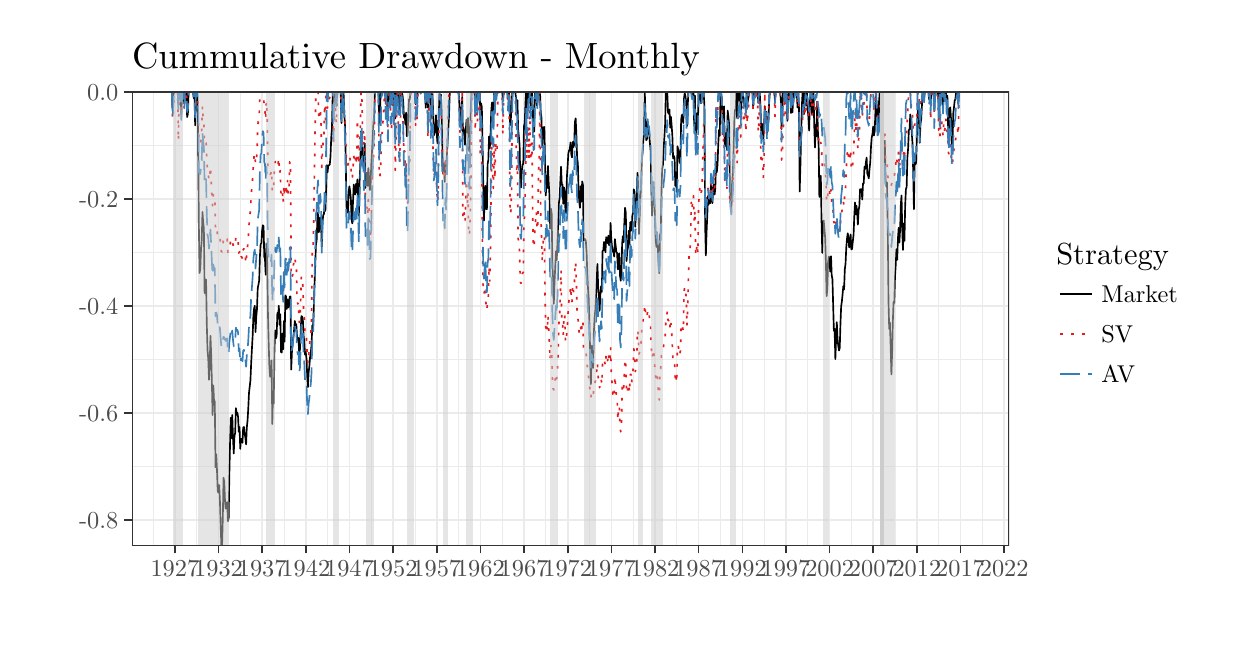
\begin{tikzpicture}[x=1pt,y=1pt]
\definecolor{fillColor}{RGB}{255,255,255}
\path[use as bounding box,fill=fillColor,fill opacity=0.00] (0,0) rectangle (426.79,216.81);
\begin{scope}
\path[clip] (  0.00,  0.00) rectangle (426.79,216.81);
\definecolor{drawColor}{RGB}{255,255,255}
\definecolor{fillColor}{RGB}{255,255,255}

\path[draw=drawColor,line width= 0.6pt,line join=round,line cap=round,fill=fillColor] (  0.00,  0.00) rectangle (426.79,216.81);
\end{scope}
\begin{scope}
\path[clip] ( 37.70, 29.59) rectangle (354.63,193.67);
\definecolor{fillColor}{RGB}{255,255,255}

\path[fill=fillColor] ( 37.70, 29.59) rectangle (354.63,193.67);
\definecolor{drawColor}{gray}{0.92}

\path[draw=drawColor,line width= 0.3pt,line join=round] ( 37.70, 58.23) --
	(354.63, 58.23);

\path[draw=drawColor,line width= 0.3pt,line join=round] ( 37.70, 96.93) --
	(354.63, 96.93);

\path[draw=drawColor,line width= 0.3pt,line join=round] ( 37.70,135.63) --
	(354.63,135.63);

\path[draw=drawColor,line width= 0.3pt,line join=round] ( 37.70,174.33) --
	(354.63,174.33);

\path[draw=drawColor,line width= 0.3pt,line join=round] ( 45.31, 29.59) --
	( 45.31,193.67);

\path[draw=drawColor,line width= 0.3pt,line join=round] ( 61.08, 29.59) --
	( 61.08,193.67);

\path[draw=drawColor,line width= 0.3pt,line join=round] ( 76.85, 29.59) --
	( 76.85,193.67);

\path[draw=drawColor,line width= 0.3pt,line join=round] ( 92.63, 29.59) --
	( 92.63,193.67);

\path[draw=drawColor,line width= 0.3pt,line join=round] (108.40, 29.59) --
	(108.40,193.67);

\path[draw=drawColor,line width= 0.3pt,line join=round] (124.17, 29.59) --
	(124.17,193.67);

\path[draw=drawColor,line width= 0.3pt,line join=round] (139.94, 29.59) --
	(139.94,193.67);

\path[draw=drawColor,line width= 0.3pt,line join=round] (155.72, 29.59) --
	(155.72,193.67);

\path[draw=drawColor,line width= 0.3pt,line join=round] (171.49, 29.59) --
	(171.49,193.67);

\path[draw=drawColor,line width= 0.3pt,line join=round] (187.26, 29.59) --
	(187.26,193.67);

\path[draw=drawColor,line width= 0.3pt,line join=round] (203.03, 29.59) --
	(203.03,193.67);

\path[draw=drawColor,line width= 0.3pt,line join=round] (218.81, 29.59) --
	(218.81,193.67);

\path[draw=drawColor,line width= 0.3pt,line join=round] (234.58, 29.59) --
	(234.58,193.67);

\path[draw=drawColor,line width= 0.3pt,line join=round] (250.35, 29.59) --
	(250.35,193.67);

\path[draw=drawColor,line width= 0.3pt,line join=round] (266.12, 29.59) --
	(266.12,193.67);

\path[draw=drawColor,line width= 0.3pt,line join=round] (281.90, 29.59) --
	(281.90,193.67);

\path[draw=drawColor,line width= 0.3pt,line join=round] (297.67, 29.59) --
	(297.67,193.67);

\path[draw=drawColor,line width= 0.3pt,line join=round] (313.44, 29.59) --
	(313.44,193.67);

\path[draw=drawColor,line width= 0.3pt,line join=round] (329.22, 29.59) --
	(329.22,193.67);

\path[draw=drawColor,line width= 0.3pt,line join=round] (344.99, 29.59) --
	(344.99,193.67);

\path[draw=drawColor,line width= 0.6pt,line join=round] ( 37.70, 38.88) --
	(354.63, 38.88);

\path[draw=drawColor,line width= 0.6pt,line join=round] ( 37.70, 77.58) --
	(354.63, 77.58);

\path[draw=drawColor,line width= 0.6pt,line join=round] ( 37.70,116.28) --
	(354.63,116.28);

\path[draw=drawColor,line width= 0.6pt,line join=round] ( 37.70,154.98) --
	(354.63,154.98);

\path[draw=drawColor,line width= 0.6pt,line join=round] ( 37.70,193.67) --
	(354.63,193.67);

\path[draw=drawColor,line width= 0.6pt,line join=round] ( 53.19, 29.59) --
	( 53.19,193.67);

\path[draw=drawColor,line width= 0.6pt,line join=round] ( 68.96, 29.59) --
	( 68.96,193.67);

\path[draw=drawColor,line width= 0.6pt,line join=round] ( 84.74, 29.59) --
	( 84.74,193.67);

\path[draw=drawColor,line width= 0.6pt,line join=round] (100.51, 29.59) --
	(100.51,193.67);

\path[draw=drawColor,line width= 0.6pt,line join=round] (116.28, 29.59) --
	(116.28,193.67);

\path[draw=drawColor,line width= 0.6pt,line join=round] (132.05, 29.59) --
	(132.05,193.67);

\path[draw=drawColor,line width= 0.6pt,line join=round] (147.83, 29.59) --
	(147.83,193.67);

\path[draw=drawColor,line width= 0.6pt,line join=round] (163.60, 29.59) --
	(163.60,193.67);

\path[draw=drawColor,line width= 0.6pt,line join=round] (179.37, 29.59) --
	(179.37,193.67);

\path[draw=drawColor,line width= 0.6pt,line join=round] (195.15, 29.59) --
	(195.15,193.67);

\path[draw=drawColor,line width= 0.6pt,line join=round] (210.92, 29.59) --
	(210.92,193.67);

\path[draw=drawColor,line width= 0.6pt,line join=round] (226.69, 29.59) --
	(226.69,193.67);

\path[draw=drawColor,line width= 0.6pt,line join=round] (242.46, 29.59) --
	(242.46,193.67);

\path[draw=drawColor,line width= 0.6pt,line join=round] (258.24, 29.59) --
	(258.24,193.67);

\path[draw=drawColor,line width= 0.6pt,line join=round] (274.01, 29.59) --
	(274.01,193.67);

\path[draw=drawColor,line width= 0.6pt,line join=round] (289.78, 29.59) --
	(289.78,193.67);

\path[draw=drawColor,line width= 0.6pt,line join=round] (305.56, 29.59) --
	(305.56,193.67);

\path[draw=drawColor,line width= 0.6pt,line join=round] (321.33, 29.59) --
	(321.33,193.67);

\path[draw=drawColor,line width= 0.6pt,line join=round] (337.10, 29.59) --
	(337.10,193.67);

\path[draw=drawColor,line width= 0.6pt,line join=round] (352.87, 29.59) --
	(352.87,193.67);
\definecolor{drawColor}{RGB}{0,0,0}

\path[draw=drawColor,line width= 0.6pt,line join=round] ( 52.11,193.67) --
	( 52.37,187.60) --
	( 52.63,192.50) --
	( 52.90,193.67) --
	( 53.16,193.54) --
	( 53.43,193.67) --
	( 53.70,193.67) --
	( 53.94,193.67) --
	( 54.20,193.67) --
	( 54.46,189.12) --
	( 54.73,193.67) --
	( 54.99,193.67) --
	( 55.26,193.67) --
	( 55.53,185.27) --
	( 55.79,193.67) --
	( 56.05,193.67) --
	( 56.31,192.62) --
	( 56.58,189.42) --
	( 56.85,193.67) --
	( 57.10,193.67) --
	( 57.37,193.67) --
	( 57.62,184.51) --
	( 57.89,185.65) --
	( 58.15,193.67) --
	( 58.42,193.67) --
	( 58.69,193.67) --
	( 58.95,193.67) --
	( 59.21,193.67) --
	( 59.47,193.67) --
	( 59.74,193.47) --
	( 60.01,191.31) --
	( 60.25,193.67) --
	( 60.52,181.46) --
	( 60.78,193.67) --
	( 61.05,193.67) --
	( 61.30,193.67) --
	( 61.57,183.31) --
	( 61.84,146.70) --
	( 62.10,128.11) --
	( 62.37,129.62) --
	( 62.63,136.67) --
	( 62.89,140.01) --
	( 63.16,150.23) --
	( 63.40,146.71) --
	( 63.67,144.16) --
	( 63.93,120.87) --
	( 64.20,125.61) --
	( 64.46,125.73) --
	( 64.72,109.84) --
	( 64.99,100.26) --
	( 65.25, 97.23) --
	( 65.52, 89.61) --
	( 65.78, 95.19) --
	( 66.05,105.46) --
	( 66.31, 98.70) --
	( 66.56, 88.79) --
	( 66.82, 76.83) --
	( 67.08, 87.52) --
	( 67.35, 81.64) --
	( 67.61, 81.83) --
	( 67.88, 57.97) --
	( 68.14, 62.67) --
	( 68.40, 57.12) --
	( 68.67, 49.39) --
	( 68.93, 48.79) --
	( 69.20, 51.53) --
	( 69.47, 45.75) --
	( 69.72, 37.49) --
	( 69.98, 29.75) --
	( 70.24, 29.59) --
	( 70.51, 39.58) --
	( 70.77, 54.20) --
	( 71.04, 52.64) --
	( 71.31, 45.67) --
	( 71.56, 43.01) --
	( 71.83, 44.94) --
	( 72.09, 45.37) --
	( 72.36, 38.44) --
	( 72.63, 39.70) --
	( 72.87, 55.30) --
	( 73.14, 67.02) --
	( 73.40, 75.86) --
	( 73.66, 68.54) --
	( 73.92, 76.82) --
	( 74.19, 68.69) --
	( 74.46, 62.94) --
	( 74.72, 69.20) --
	( 74.98, 70.43) --
	( 75.24, 79.32) --
	( 75.51, 77.38) --
	( 75.78, 77.68) --
	( 76.02, 76.25) --
	( 76.29, 70.73) --
	( 76.55, 72.51) --
	( 76.82, 64.60) --
	( 77.07, 68.27) --
	( 77.34, 68.10) --
	( 77.61, 66.81) --
	( 77.87, 72.27) --
	( 78.14, 72.52) --
	( 78.40, 70.09) --
	( 78.66, 68.73) --
	( 78.93, 66.25) --
	( 79.17, 72.21) --
	( 79.44, 74.70) --
	( 79.70, 79.00) --
	( 79.97, 84.83) --
	( 80.23, 87.09) --
	( 80.49, 89.35) --
	( 80.76, 95.53) --
	( 81.02,100.56) --
	( 81.29,105.26) --
	( 81.55,112.55) --
	( 81.82,115.39) --
	( 82.08,116.33) --
	( 82.33,106.85) --
	( 82.60,112.38) --
	( 82.86,115.13) --
	( 83.13,122.68) --
	( 83.39,123.99) --
	( 83.66,125.45) --
	( 83.92,134.19) --
	( 84.18,138.58) --
	( 84.45,138.94) --
	( 84.71,143.54) --
	( 84.98,145.42) --
	( 85.24,145.01) --
	( 85.49,134.06) --
	( 85.75,133.10) --
	( 86.01,127.51) --
	( 86.28,138.85) --
	( 86.54,132.11) --
	( 86.81,114.05) --
	( 87.08,103.12) --
	( 87.33, 94.53) --
	( 87.60, 90.67) --
	( 87.86, 91.26) --
	( 88.13, 96.55) --
	( 88.40, 73.57) --
	( 88.64, 84.28) --
	( 88.91, 81.01) --
	( 89.17,100.23) --
	( 89.43,107.44) --
	( 89.69,104.53) --
	( 89.96,105.47) --
	( 90.23,113.78) --
	( 90.49,111.69) --
	( 90.75,116.35) --
	( 91.01,109.40) --
	( 91.28,113.25) --
	( 91.55, 99.61) --
	( 91.79, 99.41) --
	( 92.06,106.27) --
	( 92.32,100.58) --
	( 92.59,110.83) --
	( 92.84,103.38) --
	( 93.11,120.08) --
	( 93.38,119.59) --
	( 93.64,115.14) --
	( 93.91,118.55) --
	( 94.17,115.69) --
	( 94.43,117.39) --
	( 94.70,119.58) --
	( 94.95,119.68) --
	( 95.22, 93.25) --
	( 95.48, 99.48) --
	( 95.75,102.67) --
	( 96.01,105.16) --
	( 96.27,107.57) --
	( 96.54,110.82) --
	( 96.80,108.97) --
	( 97.07,109.68) --
	( 97.33,105.17) --
	( 97.60,103.72) --
	( 97.86,104.72) --
	( 98.10, 99.08) --
	( 98.37,100.37) --
	( 98.63,106.24) --
	( 98.90,112.56) --
	( 99.16,112.43) --
	( 99.43,111.54) --
	( 99.69,105.63) --
	( 99.95,103.49) --
	(100.22, 98.66) --
	(100.48, 99.55) --
	(100.75, 97.19) --
	(101.02, 90.85) --
	(101.26, 86.89) --
	(101.52, 92.10) --
	(101.78, 94.46) --
	(102.05, 97.76) --
	(102.31, 99.53) --
	(102.58,102.19) --
	(102.85,109.21) --
	(103.11,109.30) --
	(103.37,114.87) --
	(103.63,123.25) --
	(103.90,130.65) --
	(104.17,138.67) --
	(104.41,139.64) --
	(104.68,147.57) --
	(104.94,150.08) --
	(105.20,142.88) --
	(105.46,144.75) --
	(105.73,148.19) --
	(106.00,146.43) --
	(106.26,137.63) --
	(106.53,146.42) --
	(106.78,149.01) --
	(107.05,149.48) --
	(107.32,153.13) --
	(107.57,150.56) --
	(107.84,158.19) --
	(108.10,167.12) --
	(108.36,164.53) --
	(108.62,167.05) --
	(108.89,167.07) --
	(109.16,167.37) --
	(109.42,170.13) --
	(109.69,177.05) --
	(109.95,180.58) --
	(110.21,192.17) --
	(110.48,184.59) --
	(110.72,193.67) --
	(110.99,193.67) --
	(111.25,193.67) --
	(111.52,189.35) --
	(111.78,193.67) --
	(112.04,193.67) --
	(112.31,193.67) --
	(112.57,193.67) --
	(112.84,193.67) --
	(113.10,193.67) --
	(113.37,182.35) --
	(113.63,192.84) --
	(113.87,193.67) --
	(114.14,193.67) --
	(114.40,186.14) --
	(114.67,181.19) --
	(114.93,169.47) --
	(115.20,152.15) --
	(115.46,149.96) --
	(115.72,150.02) --
	(115.99,157.48) --
	(116.25,159.49) --
	(116.52,157.68) --
	(116.79,154.99) --
	(117.03,147.56) --
	(117.30,146.10) --
	(117.55,153.82) --
	(117.82,160.12) --
	(118.08,157.30) --
	(118.35,156.52) --
	(118.62,160.35) --
	(118.88,157.26) --
	(119.14,161.98) --
	(119.40,155.76) --
	(119.67,148.88) --
	(119.94,161.06) --
	(120.19,167.07) --
	(120.46,179.32) --
	(120.72,179.12) --
	(120.98,169.99) --
	(121.24,170.47) --
	(121.51,165.26) --
	(121.78,175.06) --
	(122.04,158.90) --
	(122.30,164.00) --
	(122.56,164.44) --
	(122.83,159.64) --
	(123.10,166.09) --
	(123.34,162.97) --
	(123.61,158.17) --
	(123.87,158.37) --
	(124.14,167.12) --
	(124.39,171.45) --
	(124.66,176.78) --
	(124.93,182.23) --
	(125.19,185.44) --
	(125.46,193.67) --
	(125.72,193.67) --
	(125.98,193.67) --
	(126.25,193.67) --
	(126.49,193.67) --
	(126.76,193.67) --
	(127.02,182.28) --
	(127.29,185.04) --
	(127.55,193.67) --
	(127.81,193.67) --
	(128.08,193.25) --
	(128.34,193.67) --
	(128.61,193.67) --
	(128.87,193.67) --
	(129.14,193.67) --
	(129.40,189.34) --
	(129.65,193.67) --
	(129.91,189.12) --
	(130.17,184.06) --
	(130.44,193.67) --
	(130.70,193.67) --
	(130.97,193.67) --
	(131.23,189.05) --
	(131.49,189.99) --
	(131.76,193.67) --
	(132.02,193.67) --
	(132.29,188.58) --
	(132.56,193.67) --
	(132.81,183.94) --
	(133.07,189.77) --
	(133.33,193.67) --
	(133.60,193.67) --
	(133.86,192.08) --
	(134.13,188.13) --
	(134.40,186.85) --
	(134.65,193.67) --
	(134.92,193.67) --
	(135.18,193.16) --
	(135.45,192.50) --
	(135.72,189.73) --
	(135.96,184.22) --
	(136.23,185.16) --
	(136.49,181.84) --
	(136.75,186.09) --
	(137.01,177.58) --
	(137.28,177.84) --
	(137.55,185.97) --
	(137.81,190.96) --
	(138.07,190.84) --
	(138.33,193.67) --
	(138.60,193.67) --
	(138.87,193.67) --
	(139.11,193.67) --
	(139.38,193.67) --
	(139.64,193.67) --
	(139.91,193.67) --
	(140.16,189.16) --
	(140.43,193.67) --
	(140.70,190.44) --
	(140.96,193.67) --
	(141.23,193.67) --
	(141.49,193.67) --
	(141.75,193.67) --
	(142.02,193.33) --
	(142.26,193.67) --
	(142.53,193.67) --
	(142.79,193.67) --
	(143.06,193.67) --
	(143.32,193.67) --
	(143.58,193.09) --
	(143.85,187.83) --
	(144.11,193.67) --
	(144.38,193.67) --
	(144.64,187.91) --
	(144.91,193.67) --
	(145.17,193.67) --
	(145.42,193.67) --
	(145.69,183.86) --
	(145.95,190.34) --
	(146.22,193.67) --
	(146.48,187.53) --
	(146.75,177.85) --
	(147.01,178.84) --
	(147.27,179.35) --
	(147.54,185.15) --
	(147.80,178.85) --
	(148.07,175.09) --
	(148.33,178.83) --
	(148.58,186.45) --
	(148.84,192.84) --
	(149.10,191.39) --
	(149.37,192.60) --
	(149.63,182.53) --
	(149.90,171.51) --
	(150.17,164.04) --
	(150.42,167.80) --
	(150.69,161.07) --
	(150.95,168.57) --
	(151.22,165.78) --
	(151.49,170.88) --
	(151.73,175.93) --
	(152.00,180.09) --
	(152.26,185.25) --
	(152.52,193.33) --
	(152.78,193.67) --
	(153.05,193.67) --
	(153.32,193.67) --
	(153.58,193.67) --
	(153.85,193.67) --
	(154.10,193.67) --
	(154.37,193.67) --
	(154.64,193.67) --
	(154.88,193.67) --
	(155.15,193.67) --
	(155.41,193.42) --
	(155.68,193.67) --
	(155.94,190.79) --
	(156.20,181.76) --
	(156.47,184.27) --
	(156.73,187.11) --
	(157.00,191.78) --
	(157.26,178.62) --
	(157.52,180.58) --
	(157.79,177.68) --
	(158.04,174.47) --
	(158.31,179.78) --
	(158.57,183.53) --
	(158.84,178.89) --
	(159.10,184.20) --
	(159.36,173.18) --
	(159.63,172.07) --
	(159.89,180.14) --
	(160.16,188.46) --
	(160.42,193.67) --
	(160.69,193.67) --
	(160.95,193.67) --
	(161.19,193.67) --
	(161.46,193.67) --
	(161.72,187.84) --
	(161.99,193.12) --
	(162.25,193.67) --
	(162.52,189.47) --
	(162.78,193.67) --
	(163.04,193.67) --
	(163.31,193.45) --
	(163.57,186.18) --
	(163.84,189.45) --
	(164.11,188.11) --
	(164.35,175.84) --
	(164.61,160.65) --
	(164.87,147.07) --
	(165.14,156.31) --
	(165.40,159.65) --
	(165.67,151.24) --
	(165.94,151.22) --
	(166.20,167.51) --
	(166.46,169.07) --
	(166.72,177.47) --
	(166.99,173.19) --
	(167.26,178.44) --
	(167.50,186.46) --
	(167.77,189.76) --
	(168.03,185.88) --
	(168.29,185.12) --
	(168.55,193.67) --
	(168.82,190.86) --
	(169.09,193.67) --
	(169.35,192.08) --
	(169.62,193.67) --
	(169.87,193.67) --
	(170.14,193.67) --
	(170.41,193.67) --
	(170.66,193.67) --
	(170.93,193.67) --
	(171.19,193.67) --
	(171.46,193.67) --
	(171.71,190.92) --
	(171.98,193.67) --
	(172.25,193.67) --
	(172.51,193.67) --
	(172.78,193.67) --
	(173.04,193.67) --
	(173.30,193.67) --
	(173.57,191.26) --
	(173.81,193.67) --
	(174.08,192.14) --
	(174.34,181.62) --
	(174.61,184.09) --
	(174.87,189.11) --
	(175.13,193.67) --
	(175.40,193.67) --
	(175.66,193.67) --
	(175.93,193.67) --
	(176.19,193.67) --
	(176.46,191.38) --
	(176.72,186.67) --
	(176.97,190.63) --
	(177.23,179.94) --
	(177.49,177.49) --
	(177.76,174.49) --
	(178.02,160.74) --
	(178.29,159.06) --
	(178.55,165.11) --
	(178.81,167.33) --
	(179.08,167.61) --
	(179.34,181.21) --
	(179.61,182.46) --
	(179.88,189.56) --
	(180.12,193.67) --
	(180.39,185.35) --
	(180.64,189.72) --
	(180.91,193.67) --
	(181.17,191.94) --
	(181.44,193.67) --
	(181.71,187.79) --
	(181.97,188.66) --
	(182.23,193.67) --
	(182.49,185.98) --
	(182.76,179.14) --
	(183.03,179.34) --
	(183.28,193.67) --
	(183.55,193.67) --
	(183.81,193.67) --
	(184.07,188.57) --
	(184.33,191.14) --
	(184.60,193.67) --
	(184.87,193.67) --
	(185.13,193.67) --
	(185.39,186.30) --
	(185.65,184.28) --
	(185.92,173.66) --
	(186.19,178.01) --
	(186.43,180.83) --
	(186.70,180.91) --
	(186.96,167.84) --
	(187.23,156.16) --
	(187.48,163.36) --
	(187.75,158.84) --
	(188.02,166.83) --
	(188.28,160.48) --
	(188.55,156.38) --
	(188.81,144.19) --
	(189.07,151.39) --
	(189.34,149.78) --
	(189.58,133.20) --
	(189.85,123.93) --
	(190.11,117.03) --
	(190.38,125.03) --
	(190.64,130.53) --
	(190.90,136.01) --
	(191.17,132.84) --
	(191.43,138.78) --
	(191.70,146.53) --
	(191.96,153.43) --
	(192.23,155.37) --
	(192.49,161.71) --
	(192.74,166.55) --
	(193.00,160.01) --
	(193.26,160.06) --
	(193.53,153.18) --
	(193.79,159.09) --
	(194.06,157.66) --
	(194.32,150.55) --
	(194.58,149.81) --
	(194.85,162.86) --
	(195.11,166.86) --
	(195.38,171.45) --
	(195.65,172.45) --
	(195.90,172.96) --
	(196.16,175.32) --
	(196.42,171.16) --
	(196.69,169.93) --
	(196.95,175.52) --
	(197.22,173.64) --
	(197.49,174.64) --
	(197.74,182.70) --
	(198.01,184.02) --
	(198.27,178.31) --
	(198.54,169.78) --
	(198.81,167.71) --
	(199.05,158.39) --
	(199.32,153.81) --
	(199.58,151.69) --
	(199.84,159.51) --
	(200.10,154.00) --
	(200.37,161.26) --
	(200.64,160.08) --
	(200.90,139.83) --
	(201.16,140.51) --
	(201.42,140.35) --
	(201.69,139.78) --
	(201.96,135.67) --
	(202.20,128.69) --
	(202.47,122.61) --
	(202.73,118.91) --
	(203.00,109.68) --
	(203.25, 99.47) --
	(203.52, 87.96) --
	(203.79,101.89) --
	(204.05, 96.93) --
	(204.32, 93.84) --
	(204.58,106.53) --
	(204.84,111.96) --
	(205.11,114.67) --
	(205.35,119.48) --
	(205.62,125.54) --
	(205.88,131.42) --
	(206.15,122.95) --
	(206.41,119.57) --
	(206.67,114.48) --
	(206.94,120.29) --
	(207.20,123.39) --
	(207.47,121.36) --
	(207.73,136.07) --
	(208.00,136.41) --
	(208.26,139.40) --
	(208.51,137.49) --
	(208.78,135.66) --
	(209.04,141.10) --
	(209.31,139.71) --
	(209.57,138.92) --
	(209.84,141.65) --
	(210.10,138.19) --
	(210.36,138.32) --
	(210.63,146.23) --
	(210.89,140.36) --
	(211.16,137.60) --
	(211.43,135.84) --
	(211.67,136.04) --
	(211.93,134.07) --
	(212.19,140.41) --
	(212.46,138.10) --
	(212.72,135.72) --
	(212.99,135.37) --
	(213.26,129.49) --
	(213.52,134.78) --
	(213.78,135.23) --
	(214.04,127.14) --
	(214.31,125.35) --
	(214.58,128.97) --
	(214.82,139.01) --
	(215.09,141.48) --
	(215.35,139.21) --
	(215.61,146.36) --
	(215.87,151.73) --
	(216.14,149.85) --
	(216.41,132.49) --
	(216.67,136.12) --
	(216.94,137.59) --
	(217.19,143.39) --
	(217.46,138.48) --
	(217.73,146.43) --
	(217.97,146.60) --
	(218.24,143.46) --
	(218.50,148.98) --
	(218.77,149.98) --
	(219.03,158.40) --
	(219.29,157.41) --
	(219.56,144.87) --
	(219.82,152.81) --
	(220.09,155.76) --
	(220.35,164.34) --
	(220.61,162.96) --
	(220.88,142.26) --
	(221.13,148.37) --
	(221.40,155.39) --
	(221.66,159.24) --
	(221.93,168.92) --
	(222.19,171.85) --
	(222.45,175.98) --
	(222.72,178.37) --
	(222.98,193.67) --
	(223.25,185.26) --
	(223.51,176.15) --
	(223.78,176.57) --
	(224.04,182.82) --
	(224.28,178.85) --
	(224.55,179.10) --
	(224.81,175.38) --
	(225.08,172.85) --
	(225.34,160.97) --
	(225.61,148.87) --
	(225.87,155.82) --
	(226.13,160.96) --
	(226.40,154.58) --
	(226.66,148.94) --
	(226.93,140.12) --
	(227.20,137.60) --
	(227.44,142.24) --
	(227.71,136.90) --
	(227.96,132.14) --
	(228.23,128.07) --
	(228.49,141.93) --
	(228.76,142.81) --
	(229.03,158.53) --
	(229.29,165.90) --
	(229.55,167.32) --
	(229.81,173.23) --
	(230.08,177.27) --
	(230.35,182.16) --
	(230.59,193.67) --
	(230.86,193.67) --
	(231.12,193.67) --
	(231.38,186.28) --
	(231.64,185.68) --
	(231.91,187.28) --
	(232.18,180.65) --
	(232.44,184.59) --
	(232.71,181.28) --
	(232.96,177.68) --
	(233.23,169.51) --
	(233.50,170.48) --
	(233.75,169.71) --
	(234.02,159.67) --
	(234.28,162.09) --
	(234.55,157.52) --
	(234.80,173.95) --
	(235.07,172.61) --
	(235.34,171.18) --
	(235.60,167.91) --
	(235.87,170.17) --
	(236.13,183.41) --
	(236.39,185.32) --
	(236.66,183.80) --
	(236.90,182.34) --
	(237.17,191.32) --
	(237.43,193.20) --
	(237.70,191.88) --
	(237.96,189.92) --
	(238.22,181.24) --
	(238.49,188.25) --
	(238.75,193.67) --
	(239.02,193.67) --
	(239.28,193.67) --
	(239.55,193.67) --
	(239.81,193.67) --
	(240.06,191.13) --
	(240.32,193.67) --
	(240.58,193.67) --
	(240.85,181.24) --
	(241.11,192.22) --
	(241.38,176.13) --
	(241.64,183.96) --
	(241.90,185.90) --
	(242.17,180.17) --
	(242.43,193.67) --
	(242.70,193.67) --
	(242.97,193.67) --
	(243.21,189.57) --
	(243.48,189.65) --
	(243.73,193.67) --
	(244.00,193.67) --
	(244.26,193.67) --
	(244.53,188.79) --
	(244.80,145.60) --
	(245.06,134.49) --
	(245.32,143.07) --
	(245.58,148.97) --
	(245.85,156.05) --
	(246.12,153.02) --
	(246.37,153.99) --
	(246.64,153.39) --
	(246.90,160.53) --
	(247.16,158.56) --
	(247.42,153.37) --
	(247.69,158.26) --
	(247.96,160.11) --
	(248.22,156.52) --
	(248.48,158.84) --
	(248.74,168.37) --
	(249.01,164.57) --
	(249.28,167.18) --
	(249.52,174.17) --
	(249.79,179.81) --
	(250.05,177.75) --
	(250.32,189.94) --
	(250.57,192.78) --
	(250.84,191.15) --
	(251.11,184.20) --
	(251.37,186.27) --
	(251.64,188.39) --
	(251.90,174.00) --
	(252.16,175.52) --
	(252.43,178.73) --
	(252.67,172.70) --
	(252.94,186.85) --
	(253.20,184.79) --
	(253.47,181.82) --
	(253.73,164.09) --
	(253.99,154.22) --
	(254.26,151.30) --
	(254.52,160.27) --
	(254.79,163.88) --
	(255.05,170.94) --
	(255.32,182.80) --
	(255.58,187.11) --
	(255.83,186.83) --
	(256.09,193.58) --
	(256.35,184.09) --
	(256.62,191.80) --
	(256.88,193.67) --
	(257.15,190.62) --
	(257.41,193.12) --
	(257.67,185.08) --
	(257.94,193.67) --
	(258.20,192.70) --
	(258.47,193.67) --
	(258.74,188.45) --
	(258.99,190.44) --
	(259.25,191.02) --
	(259.51,186.74) --
	(259.78,193.65) --
	(260.04,189.01) --
	(260.31,190.77) --
	(260.58,192.37) --
	(260.83,193.67) --
	(261.10,193.67) --
	(261.36,193.67) --
	(261.63,193.67) --
	(261.90,193.67) --
	(262.14,188.35) --
	(262.41,193.43) --
	(262.67,193.67) --
	(262.93,193.10) --
	(263.19,193.67) --
	(263.46,193.34) --
	(263.73,193.67) --
	(263.99,189.78) --
	(264.26,193.05) --
	(264.51,193.67) --
	(264.78,188.55) --
	(265.05,179.48) --
	(265.29,180.80) --
	(265.56,182.00) --
	(265.82,176.45) --
	(266.09,181.29) --
	(266.35,188.42) --
	(266.61,184.45) --
	(266.88,186.43) --
	(267.14,178.84) --
	(267.41,180.41) --
	(267.67,183.41) --
	(267.93,189.83) --
	(268.20,193.67) --
	(268.44,193.67) --
	(268.71,193.67) --
	(268.97,193.67) --
	(269.24,193.67) --
	(269.50,193.67) --
	(269.77,193.67) --
	(270.03,190.59) --
	(270.29,193.67) --
	(270.56,193.67) --
	(270.82,193.67) --
	(271.09,193.67) --
	(271.35,193.67) --
	(271.60,193.67) --
	(271.87,193.67) --
	(272.13,191.19) --
	(272.40,180.16) --
	(272.66,185.25) --
	(272.93,193.67) --
	(273.19,193.67) --
	(273.45,193.67) --
	(273.72,190.67) --
	(273.98,193.67) --
	(274.25,192.57) --
	(274.52,183.12) --
	(274.76,190.13) --
	(275.02,193.67) --
	(275.28,193.67) --
	(275.55,193.67) --
	(275.81,185.97) --
	(276.08,193.67) --
	(276.35,186.25) --
	(276.61,191.07) --
	(276.87,193.65) --
	(277.13,193.67) --
	(277.40,193.67) --
	(277.67,193.67) --
	(277.91,193.67) --
	(278.18,187.96) --
	(278.44,193.13) --
	(278.70,187.87) --
	(278.96,157.60) --
	(279.23,166.98) --
	(279.50,178.62) --
	(279.76,188.82) --
	(280.03,193.67) --
	(280.28,193.67) --
	(280.55,185.60) --
	(280.82,191.96) --
	(281.06,193.67) --
	(281.33,188.86) --
	(281.59,193.67) --
	(281.86,187.10) --
	(282.12,184.49) --
	(282.38,179.60) --
	(282.65,190.01) --
	(282.91,193.67) --
	(283.18,193.67) --
	(283.44,185.34) --
	(283.70,190.39) --
	(283.97,193.67) --
	(284.22,181.38) --
	(284.49,173.52) --
	(284.75,181.63) --
	(285.02,177.53) --
	(285.28,190.07) --
	(285.54,179.50) --
	(285.81,174.24) --
	(286.07,155.63) --
	(286.34,157.92) --
	(286.60,163.33) --
	(286.87,146.43) --
	(287.13,135.41) --
	(287.38,146.19) --
	(287.64,147.10) --
	(287.90,143.96) --
	(288.17,140.88) --
	(288.43,132.21) --
	(288.70,119.77) --
	(288.96,122.72) --
	(289.22,132.00) --
	(289.49,134.06) --
	(289.75,131.70) --
	(290.02,128.65) --
	(290.29,134.21) --
	(290.53,127.39) --
	(290.80,125.89) --
	(291.05,116.88) --
	(291.32,107.26) --
	(291.58,107.98) --
	(291.85, 97.06) --
	(292.12,104.17) --
	(292.38,110.39) --
	(292.64,104.37) --
	(292.90,101.81) --
	(293.17,100.14) --
	(293.44,101.07) --
	(293.68,109.32) --
	(293.95,116.13) --
	(294.21,117.91) --
	(294.47,120.52) --
	(294.73,123.40) --
	(295.00,122.19) --
	(295.27,129.46) --
	(295.53,131.50) --
	(295.80,137.38) --
	(296.05,140.44) --
	(296.32,142.50) --
	(296.59,140.88) --
	(296.84,137.39) --
	(297.11,139.19) --
	(297.37,142.08) --
	(297.64,136.66) --
	(297.89,136.92) --
	(298.16,139.59) --
	(298.43,141.91) --
	(298.69,148.58) --
	(298.96,153.63) --
	(299.22,149.33) --
	(299.48,152.47) --
	(299.75,149.65) --
	(299.99,145.66) --
	(300.26,150.86) --
	(300.52,152.28) --
	(300.79,158.49) --
	(301.05,157.19) --
	(301.31,158.47) --
	(301.58,154.70) --
	(301.84,160.47) --
	(302.11,160.59) --
	(302.37,166.50) --
	(302.64,165.70) --
	(302.90,168.26) --
	(303.15,169.87) --
	(303.41,163.99) --
	(303.67,163.34) --
	(303.94,162.34) --
	(304.20,165.74) --
	(304.47,168.28) --
	(304.73,173.79) --
	(304.99,177.18) --
	(305.26,178.37) --
	(305.52,181.07) --
	(305.79,177.83) --
	(306.06,179.34) --
	(306.30,185.77) --
	(306.57,192.17) --
	(306.82,188.51) --
	(307.09,181.78) --
	(307.35,183.16) --
	(307.62,189.88) --
	(307.89,193.67) --
	(308.15,183.54) --
	(308.41,182.15) --
	(308.67,170.26) --
	(308.94,166.13) --
	(309.21,164.06) --
	(309.46,172.21) --
	(309.73,176.01) --
	(309.99,161.93) --
	(310.25,159.49) --
	(310.51,160.90) --
	(310.78,144.93) --
	(311.05,118.05) --
	(311.31,107.92) --
	(311.57,110.21) --
	(311.83,101.68) --
	(312.10, 91.50) --
	(312.37, 99.42) --
	(312.61,110.26) --
	(312.88,117.70) --
	(313.14,117.33) --
	(313.41,126.90) --
	(313.66,130.87) --
	(313.93,136.77) --
	(314.20,132.93) --
	(314.46,140.50) --
	(314.73,144.48) --
	(314.99,139.13) --
	(315.25,143.95) --
	(315.52,153.09) --
	(315.76,156.16) --
	(316.03,143.80) --
	(316.29,136.50) --
	(316.56,146.07) --
	(316.82,139.81) --
	(317.08,152.57) --
	(317.35,158.43) --
	(317.61,159.22) --
	(317.88,169.88) --
	(318.14,173.12) --
	(318.41,179.70) --
	(318.67,180.29) --
	(318.92,185.43) --
	(319.18,182.65) --
	(319.44,179.29) --
	(319.71,175.27) --
	(319.97,165.21) --
	(320.24,151.20) --
	(320.51,168.40) --
	(320.76,167.35) --
	(321.03,167.97) --
	(321.29,177.04) --
	(321.56,184.32) --
	(321.83,188.74) --
	(322.08,187.46) --
	(322.34,175.19) --
	(322.60,181.87) --
	(322.87,183.71) --
	(323.13,188.53) --
	(323.40,193.53) --
	(323.67,190.79) --
	(323.93,191.95) --
	(324.19,193.67) --
	(324.45,193.67) --
	(324.72,193.67) --
	(324.99,193.67) --
	(325.23,193.67) --
	(325.50,193.67) --
	(325.76,190.76) --
	(326.02,193.67) --
	(326.28,188.70) --
	(326.55,193.67) --
	(326.82,193.67) --
	(327.08,193.67) --
	(327.35,193.67) --
	(327.60,187.88) --
	(327.87,193.67) --
	(328.14,193.67) --
	(328.38,193.67) --
	(328.65,193.67) --
	(328.91,193.67) --
	(329.18,189.70) --
	(329.44,193.67) --
	(329.70,188.81) --
	(329.97,192.81) --
	(330.23,193.67) --
	(330.50,192.98) --
	(330.76,187.74) --
	(331.02,193.67) --
	(331.29,191.65) --
	(331.53,193.33) --
	(331.80,193.67) --
	(332.06,189.95) --
	(332.33,192.24) --
	(332.59,180.72) --
	(332.86,174.63) --
	(333.12,187.53) --
	(333.38,187.99) --
	(333.65,183.81) --
	(333.91,173.34) --
	(334.18,173.44) --
	(334.44,185.63) --
	(334.69,187.78) --
	(334.96,190.42) --
	(335.22,191.00) --
	(335.49,193.67) --
	(335.75,193.67) --
	(336.02,193.67) --
	(336.28,189.46) --
	(336.54,193.67) --
	(336.81,193.67) --
	(337.07,193.67) --
	(337.34,193.67) --
	(337.61,193.67) --
	(337.85,193.67) --
	(338.12,193.67) --
	(338.37,193.67) --
	(338.64,193.67) --
	(338.90,193.67) --
	(339.17,193.67) --
	(339.44,193.67) --
	(339.70,193.67) --
	(339.96,193.67) --
	(340.22,193.67);
\definecolor{drawColor}{RGB}{228,26,28}

\path[draw=drawColor,line width= 0.6pt,dash pattern=on 1pt off 3pt ,line join=round] ( 52.11,193.67) --
	( 52.37,183.67) --
	( 52.63,186.35) --
	( 52.90,193.67) --
	( 53.16,193.37) --
	( 53.43,193.67) --
	( 53.70,193.67) --
	( 53.94,193.67) --
	( 54.20,193.67) --
	( 54.46,175.98) --
	( 54.73,191.84) --
	( 54.99,193.67) --
	( 55.26,193.67) --
	( 55.53,185.05) --
	( 55.79,193.67) --
	( 56.05,193.67) --
	( 56.31,191.71) --
	( 56.58,188.01) --
	( 56.85,193.67) --
	( 57.10,193.67) --
	( 57.37,193.67) --
	( 57.62,188.55) --
	( 57.89,188.82) --
	( 58.15,193.67) --
	( 58.42,193.67) --
	( 58.69,193.67) --
	( 58.95,193.67) --
	( 59.21,193.67) --
	( 59.47,193.67) --
	( 59.74,193.53) --
	( 60.01,192.78) --
	( 60.25,193.38) --
	( 60.52,187.41) --
	( 60.78,191.92) --
	( 61.05,193.67) --
	( 61.30,193.67) --
	( 61.57,190.10) --
	( 61.84,175.35) --
	( 62.10,174.96) --
	( 62.37,175.02) --
	( 62.63,176.01) --
	( 62.89,180.06) --
	( 63.16,188.55) --
	( 63.40,184.08) --
	( 63.67,182.01) --
	( 63.93,175.07) --
	( 64.20,175.63) --
	( 64.46,175.67) --
	( 64.72,169.60) --
	( 64.99,164.27) --
	( 65.25,163.80) --
	( 65.52,161.72) --
	( 65.78,163.05) --
	( 66.05,166.58) --
	( 66.31,161.37) --
	( 66.56,156.32) --
	( 66.82,152.47) --
	( 67.08,156.50) --
	( 67.35,155.90) --
	( 67.61,155.96) --
	( 67.88,143.21) --
	( 68.14,143.91) --
	( 68.40,143.54) --
	( 68.67,141.42) --
	( 68.93,141.33) --
	( 69.20,141.84) --
	( 69.47,141.08) --
	( 69.72,138.31) --
	( 69.98,135.88) --
	( 70.24,135.83) --
	( 70.51,137.47) --
	( 70.77,140.95) --
	( 71.04,140.79) --
	( 71.31,140.25) --
	( 71.56,139.97) --
	( 71.83,140.28) --
	( 72.09,140.45) --
	( 72.36,135.58) --
	( 72.63,135.99) --
	( 72.87,137.28) --
	( 73.14,138.51) --
	( 73.40,140.15) --
	( 73.66,139.42) --
	( 73.92,139.89) --
	( 74.19,138.43) --
	( 74.46,137.46) --
	( 74.72,138.02) --
	( 74.98,138.32) --
	( 75.24,141.32) --
	( 75.51,140.71) --
	( 75.78,140.82) --
	( 76.02,140.35) --
	( 76.29,135.35) --
	( 76.55,135.87) --
	( 76.82,133.24) --
	( 77.07,134.02) --
	( 77.34,133.96) --
	( 77.61,133.32) --
	( 77.87,136.58) --
	( 78.14,136.95) --
	( 78.40,134.95) --
	( 78.66,133.63) --
	( 78.93,131.64) --
	( 79.17,135.48) --
	( 79.44,137.59) --
	( 79.70,140.63) --
	( 79.97,145.29) --
	( 80.23,148.94) --
	( 80.49,150.48) --
	( 80.76,156.13) --
	( 81.02,159.31) --
	( 81.29,162.27) --
	( 81.55,167.46) --
	( 81.82,170.48) --
	( 82.08,171.29) --
	( 82.33,167.63) --
	( 82.60,169.48) --
	( 82.86,171.17) --
	( 83.13,181.37) --
	( 83.39,183.30) --
	( 83.66,184.46) --
	( 83.92,193.67) --
	( 84.18,193.67) --
	( 84.45,193.67) --
	( 84.71,193.67) --
	( 84.98,193.67) --
	( 85.24,193.13) --
	( 85.49,186.76) --
	( 85.75,186.48) --
	( 86.01,183.63) --
	( 86.28,190.18) --
	( 86.54,184.95) --
	( 86.81,165.93) --
	( 87.08,164.75) --
	( 87.33,164.26) --
	( 87.60,163.86) --
	( 87.86,164.05) --
	( 88.13,165.32) --
	( 88.40,157.93) --
	( 88.64,160.10) --
	( 88.91,159.66) --
	( 89.17,166.92) --
	( 89.43,168.44) --
	( 89.69,167.55) --
	( 89.96,167.88) --
	( 90.23,168.77) --
	( 90.49,167.66) --
	( 90.75,169.75) --
	( 91.01,164.16) --
	( 91.28,165.17) --
	( 91.55,155.82) --
	( 91.79,155.78) --
	( 92.06,157.18) --
	( 92.32,153.46) --
	( 92.59,159.93) --
	( 92.84,155.82) --
	( 93.11,160.18) --
	( 93.38,160.13) --
	( 93.64,156.04) --
	( 93.91,161.53) --
	( 94.17,156.70) --
	( 94.43,158.69) --
	( 94.70,168.31) --
	( 94.95,168.55) --
	( 95.22,126.33) --
	( 95.48,126.81) --
	( 95.75,127.34) --
	( 96.01,131.08) --
	( 96.27,132.25) --
	( 96.54,133.86) --
	( 96.80,131.62) --
	( 97.07,131.81) --
	( 97.33,118.40) --
	( 97.60,116.97) --
	( 97.86,117.50) --
	( 98.10,110.28) --
	( 98.37,111.35) --
	( 98.63,118.10) --
	( 98.90,126.94) --
	( 99.16,126.77) --
	( 99.43,123.51) --
	( 99.69,115.03) --
	( 99.95,112.69) --
	(100.22,105.95) --
	(100.48,106.11) --
	(100.75,104.66) --
	(101.02, 97.62) --
	(101.26, 95.62) --
	(101.52, 98.30) --
	(101.78,100.78) --
	(102.05,104.00) --
	(102.31,105.35) --
	(102.58,112.35) --
	(102.85,137.41) --
	(103.11,137.53) --
	(103.37,147.50) --
	(103.63,165.15) --
	(103.90,183.09) --
	(104.17,193.67) --
	(104.41,193.67) --
	(104.68,193.67) --
	(104.94,193.67) --
	(105.20,183.39) --
	(105.46,184.52) --
	(105.73,187.62) --
	(106.00,183.14) --
	(106.26,166.31) --
	(106.53,171.84) --
	(106.78,175.82) --
	(107.05,176.90) --
	(107.32,189.06) --
	(107.57,183.58) --
	(107.84,193.67) --
	(108.10,193.67) --
	(108.36,187.75) --
	(108.62,191.04) --
	(108.89,191.11) --
	(109.16,191.44) --
	(109.42,193.67) --
	(109.69,193.67) --
	(109.95,193.67) --
	(110.21,193.67) --
	(110.48,174.37) --
	(110.72,182.07) --
	(110.99,186.41) --
	(111.25,187.54) --
	(111.52,182.09) --
	(111.78,189.10) --
	(112.04,193.67) --
	(112.31,193.67) --
	(112.57,193.67) --
	(112.84,193.67) --
	(113.10,193.67) --
	(113.37,188.33) --
	(113.63,190.18) --
	(113.87,193.67) --
	(114.14,193.67) --
	(114.40,186.57) --
	(114.67,183.12) --
	(114.93,176.62) --
	(115.20,167.29) --
	(115.46,167.13) --
	(115.72,167.14) --
	(115.99,169.43) --
	(116.25,170.33) --
	(116.52,169.26) --
	(116.79,166.75) --
	(117.03,163.05) --
	(117.30,162.27) --
	(117.55,166.11) --
	(117.82,170.58) --
	(118.08,168.75) --
	(118.35,167.70) --
	(118.62,171.13) --
	(118.88,167.28) --
	(119.14,183.68) --
	(119.40,175.36) --
	(119.67,167.37) --
	(119.94,175.53) --
	(120.19,179.60) --
	(120.46,193.67) --
	(120.72,193.44) --
	(120.98,180.94) --
	(121.24,181.16) --
	(121.51,174.08) --
	(121.78,178.88) --
	(122.04,151.42) --
	(122.30,152.31) --
	(122.56,152.85) --
	(122.83,148.99) --
	(123.10,154.69) --
	(123.34,151.48) --
	(123.61,140.79) --
	(123.87,141.03) --
	(124.14,146.39) --
	(124.39,159.21) --
	(124.66,165.53) --
	(124.93,169.06) --
	(125.19,174.52) --
	(125.46,190.64) --
	(125.72,193.67) --
	(125.98,193.67) --
	(126.25,193.67) --
	(126.49,193.67) --
	(126.76,193.67) --
	(127.02,162.86) --
	(127.29,163.32) --
	(127.55,165.88) --
	(127.81,179.01) --
	(128.08,178.58) --
	(128.34,182.36) --
	(128.61,186.52) --
	(128.87,190.94) --
	(129.14,192.77) --
	(129.40,184.33) --
	(129.65,191.59) --
	(129.91,185.78) --
	(130.17,181.01) --
	(130.44,193.67) --
	(130.70,193.67) --
	(130.97,193.67) --
	(131.23,180.21) --
	(131.49,180.79) --
	(131.76,188.18) --
	(132.02,193.67) --
	(132.29,180.90) --
	(132.56,190.59) --
	(132.81,165.28) --
	(133.07,173.79) --
	(133.33,189.54) --
	(133.60,193.67) --
	(133.86,186.66) --
	(134.13,170.73) --
	(134.40,167.65) --
	(134.65,179.25) --
	(134.92,193.67) --
	(135.18,189.65) --
	(135.45,187.60) --
	(135.72,179.26) --
	(135.96,171.42) --
	(136.23,172.29) --
	(136.49,165.36) --
	(136.75,168.80) --
	(137.01,152.50) --
	(137.28,152.91) --
	(137.55,158.79) --
	(137.81,168.97) --
	(138.07,168.59) --
	(138.33,192.49) --
	(138.60,193.67) --
	(138.87,193.67) --
	(139.11,193.67) --
	(139.38,193.67) --
	(139.64,193.67) --
	(139.91,193.67) --
	(140.16,180.82) --
	(140.43,193.67) --
	(140.70,182.93) --
	(140.96,193.67) --
	(141.23,193.67) --
	(141.49,193.67) --
	(141.75,193.67) --
	(142.02,192.91) --
	(142.26,193.67) --
	(142.53,193.67) --
	(142.79,193.67) --
	(143.06,193.67) --
	(143.32,193.67) --
	(143.58,192.94) --
	(143.85,191.99) --
	(144.11,193.67) --
	(144.38,193.67) --
	(144.64,176.77) --
	(144.91,183.01) --
	(145.17,193.67) --
	(145.42,193.67) --
	(145.69,181.13) --
	(145.95,185.14) --
	(146.22,193.67) --
	(146.48,171.63) --
	(146.75,162.79) --
	(147.01,164.26) --
	(147.27,164.60) --
	(147.54,168.17) --
	(147.80,158.92) --
	(148.07,153.74) --
	(148.33,156.77) --
	(148.58,178.99) --
	(148.84,193.67) --
	(149.10,190.04) --
	(149.37,192.08) --
	(149.63,174.39) --
	(149.90,169.19) --
	(150.17,163.95) --
	(150.42,164.65) --
	(150.69,162.81) --
	(150.95,168.90) --
	(151.22,165.08) --
	(151.49,172.30) --
	(151.73,182.97) --
	(152.00,189.14) --
	(152.26,193.67) --
	(152.52,193.67) --
	(152.78,193.67) --
	(153.05,193.67) --
	(153.32,193.67) --
	(153.58,193.67) --
	(153.85,193.67) --
	(154.10,193.67) --
	(154.37,193.67) --
	(154.64,193.67) --
	(154.88,193.67) --
	(155.15,193.67) --
	(155.41,193.09) --
	(155.68,193.67) --
	(155.94,187.00) --
	(156.20,179.04) --
	(156.47,180.46) --
	(156.73,184.90) --
	(157.00,193.67) --
	(157.26,148.91) --
	(157.52,151.39) --
	(157.79,149.28) --
	(158.04,146.60) --
	(158.31,153.84) --
	(158.57,161.62) --
	(158.84,152.83) --
	(159.10,157.20) --
	(159.36,142.24) --
	(159.63,141.71) --
	(159.89,147.52) --
	(160.16,159.21) --
	(160.42,190.51) --
	(160.69,193.67) --
	(160.95,193.67) --
	(161.19,193.67) --
	(161.46,193.67) --
	(161.72,179.49) --
	(161.99,189.28) --
	(162.25,193.67) --
	(162.52,182.52) --
	(162.78,188.19) --
	(163.04,193.67) --
	(163.31,192.86) --
	(163.57,170.84) --
	(163.84,174.82) --
	(164.11,169.94) --
	(164.35,134.32) --
	(164.61,121.56) --
	(164.87,120.60) --
	(165.14,121.77) --
	(165.40,123.25) --
	(165.67,114.83) --
	(165.94,114.81) --
	(166.20,118.36) --
	(166.46,119.71) --
	(166.72,130.65) --
	(166.99,125.27) --
	(167.26,136.60) --
	(167.50,159.85) --
	(167.77,176.17) --
	(168.03,161.61) --
	(168.29,158.73) --
	(168.55,175.00) --
	(168.82,162.16) --
	(169.09,175.43) --
	(169.35,171.89) --
	(169.62,172.87) --
	(169.87,191.06) --
	(170.14,193.67) --
	(170.41,193.67) --
	(170.66,193.67) --
	(170.93,193.67) --
	(171.19,193.67) --
	(171.46,193.67) --
	(171.71,178.13) --
	(171.98,191.17) --
	(172.25,193.67) --
	(172.51,193.67) --
	(172.78,193.67) --
	(173.04,193.67) --
	(173.30,193.67) --
	(173.57,187.18) --
	(173.81,193.67) --
	(174.08,178.83) --
	(174.34,149.46) --
	(174.61,150.52) --
	(174.87,158.52) --
	(175.13,193.67) --
	(175.40,193.67) --
	(175.66,193.63) --
	(175.93,193.67) --
	(176.19,193.67) --
	(176.46,177.43) --
	(176.72,164.21) --
	(176.97,167.51) --
	(177.23,140.52) --
	(177.49,139.59) --
	(177.76,135.36) --
	(178.02,124.86) --
	(178.29,124.43) --
	(178.55,127.36) --
	(178.81,128.05) --
	(179.08,128.32) --
	(179.34,146.87) --
	(179.61,149.05) --
	(179.88,162.69) --
	(180.12,179.21) --
	(180.39,169.21) --
	(180.64,174.26) --
	(180.91,181.19) --
	(181.17,169.23) --
	(181.44,187.32) --
	(181.71,168.64) --
	(181.97,170.59) --
	(182.23,175.16) --
	(182.49,148.27) --
	(182.76,137.39) --
	(183.03,137.55) --
	(183.28,144.74) --
	(183.55,147.41) --
	(183.81,150.31) --
	(184.07,143.79) --
	(184.33,145.93) --
	(184.60,165.48) --
	(184.87,170.27) --
	(185.13,193.67) --
	(185.39,149.11) --
	(185.65,143.18) --
	(185.92,132.33) --
	(186.19,138.01) --
	(186.43,141.72) --
	(186.70,141.82) --
	(186.96,119.36) --
	(187.23,108.24) --
	(187.48,110.11) --
	(187.75,107.16) --
	(188.02,112.89) --
	(188.28,107.52) --
	(188.55,102.56) --
	(188.81, 96.84) --
	(189.07,101.94) --
	(189.34,100.83) --
	(189.58, 90.63) --
	(189.85, 86.46) --
	(190.11, 85.95) --
	(190.38, 87.89) --
	(190.64, 89.83) --
	(190.90, 91.76) --
	(191.17, 89.95) --
	(191.43, 93.64) --
	(191.70, 99.24) --
	(191.96,109.97) --
	(192.23,112.90) --
	(192.49,121.18) --
	(192.74,129.31) --
	(193.00,110.20) --
	(193.26,110.26) --
	(193.53,105.59) --
	(193.79,113.25) --
	(194.06,112.87) --
	(194.32,103.91) --
	(194.58,103.14) --
	(194.85,107.36) --
	(195.11,110.36) --
	(195.38,115.95) --
	(195.65,118.80) --
	(195.90,119.37) --
	(196.16,123.29) --
	(196.42,119.94) --
	(196.69,117.47) --
	(196.95,123.82) --
	(197.22,121.42) --
	(197.49,122.81) --
	(197.74,129.52) --
	(198.01,132.17) --
	(198.27,124.13) --
	(198.54,113.77) --
	(198.81,112.61) --
	(199.05,108.62) --
	(199.32,106.43) --
	(199.58,105.99) --
	(199.84,108.54) --
	(200.10,106.39) --
	(200.37,111.08) --
	(200.64,110.03) --
	(200.90, 99.54) --
	(201.16, 99.66) --
	(201.42, 99.64) --
	(201.69, 99.51) --
	(201.96, 97.82) --
	(202.20, 94.59) --
	(202.47, 91.91) --
	(202.73, 90.48) --
	(203.00, 87.41) --
	(203.25, 85.68) --
	(203.52, 83.20) --
	(203.79, 84.94) --
	(204.05, 84.43) --
	(204.32, 83.61) --
	(204.58, 86.52) --
	(204.84, 87.86) --
	(205.11, 88.99) --
	(205.35, 90.59) --
	(205.62, 92.94) --
	(205.88, 95.72) --
	(206.15, 90.47) --
	(206.41, 88.26) --
	(206.67, 86.71) --
	(206.94, 88.67) --
	(207.20, 89.90) --
	(207.47, 87.96) --
	(207.73, 95.25) --
	(208.00, 95.44) --
	(208.26, 97.15) --
	(208.51, 95.94) --
	(208.78, 94.69) --
	(209.04, 98.97) --
	(209.31, 97.74) --
	(209.57, 96.48) --
	(209.84, 99.27) --
	(210.10, 95.99) --
	(210.36, 96.07) --
	(210.63,101.35) --
	(210.89, 91.81) --
	(211.16, 88.28) --
	(211.43, 84.41) --
	(211.67, 84.62) --
	(211.93, 83.30) --
	(212.19, 90.90) --
	(212.46, 87.07) --
	(212.72, 84.23) --
	(212.99, 83.73) --
	(213.26, 75.01) --
	(213.52, 79.89) --
	(213.78, 80.10) --
	(214.04, 72.16) --
	(214.31, 70.79) --
	(214.58, 74.57) --
	(214.82, 86.97) --
	(215.09, 88.33) --
	(215.35, 86.68) --
	(215.61, 91.62) --
	(215.87, 97.03) --
	(216.14, 95.67) --
	(216.41, 84.61) --
	(216.67, 85.81) --
	(216.94, 86.07) --
	(217.19, 88.17) --
	(217.46, 84.94) --
	(217.73, 91.38) --
	(217.97, 91.56) --
	(218.24, 88.39) --
	(218.50, 91.96) --
	(218.77, 93.28) --
	(219.03,100.78) --
	(219.29, 98.97) --
	(219.56, 92.56) --
	(219.82, 94.15) --
	(220.09, 95.39) --
	(220.35,107.52) --
	(220.61,107.01) --
	(220.88, 98.83) --
	(221.13, 99.64) --
	(221.40,101.29) --
	(221.66,103.22) --
	(221.93,108.34) --
	(222.19,110.12) --
	(222.45,111.60) --
	(222.72,112.14) --
	(222.98,116.75) --
	(223.25,113.96) --
	(223.51,112.11) --
	(223.78,112.27) --
	(224.04,114.66) --
	(224.28,113.11) --
	(224.55,113.30) --
	(224.81,110.65) --
	(225.08,109.08) --
	(225.34,101.93) --
	(225.61, 97.47) --
	(225.87, 98.92) --
	(226.13,100.58) --
	(226.40, 97.54) --
	(226.66, 93.01) --
	(226.93, 90.78) --
	(227.20, 89.67) --
	(227.44, 91.46) --
	(227.71, 87.97) --
	(227.96, 84.12) --
	(228.23, 82.29) --
	(228.49, 93.51) --
	(228.76, 93.63) --
	(229.03, 99.20) --
	(229.29,100.13) --
	(229.55,100.31) --
	(229.81,102.03) --
	(230.08,102.80) --
	(230.35,104.62) --
	(230.59,110.63) --
	(230.86,111.42) --
	(231.12,114.45) --
	(231.38,111.14) --
	(231.64,110.97) --
	(231.91,111.78) --
	(232.18,107.50) --
	(232.44,109.92) --
	(232.71,107.02) --
	(232.96,101.77) --
	(233.23, 95.75) --
	(233.50, 96.06) --
	(233.75, 95.67) --
	(234.02, 88.81) --
	(234.28, 90.52) --
	(234.55, 88.50) --
	(234.80,102.00) --
	(235.07,101.67) --
	(235.34,100.45) --
	(235.60, 98.49) --
	(235.87,100.10) --
	(236.13,108.76) --
	(236.39,109.82) --
	(236.66,108.42) --
	(236.90,107.12) --
	(237.17,121.30) --
	(237.43,123.17) --
	(237.70,121.48) --
	(237.96,119.55) --
	(238.22,108.98) --
	(238.49,115.04) --
	(238.75,126.45) --
	(239.02,135.04) --
	(239.28,135.58) --
	(239.55,141.43) --
	(239.81,153.67) --
	(240.06,151.12) --
	(240.32,154.56) --
	(240.58,156.06) --
	(240.85,146.68) --
	(241.11,150.84) --
	(241.38,134.52) --
	(241.64,136.29) --
	(241.90,138.62) --
	(242.17,135.29) --
	(242.43,152.86) --
	(242.70,156.82) --
	(242.97,159.65) --
	(243.21,157.40) --
	(243.48,157.42) --
	(243.73,160.70) --
	(244.00,171.22) --
	(244.26,181.91) --
	(244.53,178.51) --
	(244.80,154.98) --
	(245.06,154.75) --
	(245.32,156.50) --
	(245.58,157.72) --
	(245.85,158.77) --
	(246.12,156.36) --
	(246.37,157.15) --
	(246.64,156.91) --
	(246.90,160.90) --
	(247.16,159.61) --
	(247.42,155.21) --
	(247.69,159.92) --
	(247.96,162.37) --
	(248.22,158.96) --
	(248.48,161.22) --
	(248.74,188.90) --
	(249.01,181.07) --
	(249.28,184.50) --
	(249.52,192.31) --
	(249.79,193.67) --
	(250.05,190.44) --
	(250.32,193.67) --
	(250.57,193.67) --
	(250.84,191.92) --
	(251.11,175.37) --
	(251.37,175.82) --
	(251.64,178.96) --
	(251.90,161.65) --
	(252.16,162.33) --
	(252.43,166.14) --
	(252.67,158.74) --
	(252.94,175.05) --
	(253.20,172.46) --
	(253.47,169.77) --
	(253.73,154.42) --
	(253.99,152.67) --
	(254.26,150.86) --
	(254.52,153.12) --
	(254.79,154.95) --
	(255.05,165.08) --
	(255.32,169.14) --
	(255.58,171.24) --
	(255.83,171.03) --
	(256.09,174.69) --
	(256.35,168.01) --
	(256.62,176.43) --
	(256.88,181.41) --
	(257.15,179.84) --
	(257.41,184.95) --
	(257.67,177.29) --
	(257.94,186.88) --
	(258.20,186.17) --
	(258.47,188.22) --
	(258.74,182.23) --
	(258.99,186.52) --
	(259.25,186.86) --
	(259.51,179.12) --
	(259.78,188.16) --
	(260.04,182.07) --
	(260.31,187.15) --
	(260.58,189.12) --
	(260.83,193.67) --
	(261.10,193.67) --
	(261.36,193.67) --
	(261.63,193.67) --
	(261.90,193.67) --
	(262.14,186.60) --
	(262.41,192.16) --
	(262.67,193.09) --
	(262.93,191.96) --
	(263.19,193.67) --
	(263.46,191.82) --
	(263.73,193.67) --
	(263.99,178.96) --
	(264.26,183.33) --
	(264.51,193.67) --
	(264.78,176.31) --
	(265.05,167.51) --
	(265.29,168.88) --
	(265.56,169.59) --
	(265.82,162.42) --
	(266.09,168.60) --
	(266.35,193.52) --
	(266.61,182.04) --
	(266.88,185.20) --
	(267.14,177.26) --
	(267.41,179.50) --
	(267.67,184.00) --
	(267.93,193.67) --
	(268.20,193.67) --
	(268.44,193.67) --
	(268.71,193.67) --
	(268.97,193.67) --
	(269.24,193.67) --
	(269.50,193.67) --
	(269.77,193.67) --
	(270.03,184.71) --
	(270.29,193.67) --
	(270.56,193.67) --
	(270.82,193.67) --
	(271.09,193.67) --
	(271.35,193.67) --
	(271.60,193.67) --
	(271.87,193.67) --
	(272.13,190.98) --
	(272.40,168.98) --
	(272.66,170.70) --
	(272.93,179.04) --
	(273.19,182.67) --
	(273.45,193.67) --
	(273.72,185.80) --
	(273.98,192.96) --
	(274.25,191.82) --
	(274.52,183.97) --
	(274.76,188.35) --
	(275.02,193.52) --
	(275.28,193.67) --
	(275.55,193.67) --
	(275.81,187.84) --
	(276.08,193.67) --
	(276.35,189.02) --
	(276.61,189.62) --
	(276.87,190.68) --
	(277.13,190.74) --
	(277.40,193.67) --
	(277.67,193.67) --
	(277.91,193.67) --
	(278.18,190.21) --
	(278.44,193.67) --
	(278.70,190.83) --
	(278.96,174.50) --
	(279.23,175.69) --
	(279.50,177.00) --
	(279.76,178.61) --
	(280.03,184.53) --
	(280.28,186.87) --
	(280.55,184.23) --
	(280.82,186.10) --
	(281.06,188.98) --
	(281.33,187.16) --
	(281.59,190.19) --
	(281.86,187.39) --
	(282.12,185.79) --
	(282.38,183.97) --
	(282.65,188.08) --
	(282.91,189.49) --
	(283.18,193.67) --
	(283.44,185.27) --
	(283.70,186.10) --
	(283.97,189.25) --
	(284.22,187.37) --
	(284.49,186.68) --
	(284.75,187.87) --
	(285.02,186.56) --
	(285.28,191.06) --
	(285.54,179.32) --
	(285.81,176.61) --
	(286.07,174.02) --
	(286.34,174.60) --
	(286.60,175.36) --
	(286.87,172.49) --
	(287.13,167.03) --
	(287.38,168.76) --
	(287.64,168.88) --
	(287.90,167.64) --
	(288.17,165.53) --
	(288.43,161.92) --
	(288.70,153.87) --
	(288.96,154.38) --
	(289.22,157.55) --
	(289.49,158.81) --
	(289.75,157.41) --
	(290.02,155.68) --
	(290.29,158.22) --
	(290.53,154.09) --
	(290.80,153.24) --
	(291.05,150.29) --
	(291.32,146.34) --
	(291.58,146.41) --
	(291.85,144.65) --
	(292.12,146.25) --
	(292.38,147.01) --
	(292.64,145.14) --
	(292.90,143.68) --
	(293.17,143.18) --
	(293.44,143.76) --
	(293.68,145.80) --
	(293.95,149.32) --
	(294.21,150.49) --
	(294.47,152.12) --
	(294.73,153.95) --
	(295.00,152.37) --
	(295.27,157.02) --
	(295.53,158.89) --
	(295.80,165.93) --
	(296.05,170.07) --
	(296.32,172.97) --
	(296.59,170.46) --
	(296.84,168.56) --
	(297.11,170.11) --
	(297.37,172.77) --
	(297.64,165.39) --
	(297.89,165.75) --
	(298.16,167.75) --
	(298.43,171.50) --
	(298.69,178.20) --
	(298.96,186.62) --
	(299.22,179.03) --
	(299.48,183.05) --
	(299.75,179.12) --
	(299.99,173.13) --
	(300.26,176.53) --
	(300.52,178.37) --
	(300.79,192.00) --
	(301.05,189.47) --
	(301.31,191.47) --
	(301.58,184.58) --
	(301.84,187.74) --
	(302.11,187.99) --
	(302.37,193.67) --
	(302.64,192.71) --
	(302.90,193.67) --
	(303.15,193.67) --
	(303.41,183.17) --
	(303.67,182.71) --
	(303.94,182.31) --
	(304.20,184.30) --
	(304.47,189.22) --
	(304.73,193.67) --
	(304.99,193.67) --
	(305.26,193.67) --
	(305.52,193.67) --
	(305.79,187.40) --
	(306.06,188.42) --
	(306.30,192.12) --
	(306.57,193.67) --
	(306.82,188.96) --
	(307.09,184.58) --
	(307.35,185.16) --
	(307.62,186.43) --
	(307.89,188.54) --
	(308.15,183.32) --
	(308.41,183.08) --
	(308.67,178.44) --
	(308.94,177.49) --
	(309.21,176.85) --
	(309.46,178.11) --
	(309.73,179.53) --
	(309.99,169.48) --
	(310.25,168.56) --
	(310.51,168.89) --
	(310.78,163.29) --
	(311.05,161.86) --
	(311.31,161.62) --
	(311.57,161.70) --
	(311.83,161.11) --
	(312.10,159.86) --
	(312.37,161.24) --
	(312.61,162.00) --
	(312.88,163.23) --
	(313.14,163.16) --
	(313.41,166.14) --
	(313.66,167.42) --
	(313.93,170.18) --
	(314.20,168.07) --
	(314.46,170.04) --
	(314.73,172.17) --
	(314.99,166.16) --
	(315.25,168.90) --
	(315.52,172.88) --
	(315.76,178.06) --
	(316.03,171.07) --
	(316.29,170.09) --
	(316.56,171.93) --
	(316.82,169.82) --
	(317.08,174.85) --
	(317.35,177.96) --
	(317.61,178.70) --
	(317.88,184.48) --
	(318.14,189.89) --
	(318.41,193.67) --
	(318.67,193.67) --
	(318.92,193.67) --
	(319.18,189.70) --
	(319.44,186.91) --
	(319.71,185.28) --
	(319.97,180.08) --
	(320.24,179.33) --
	(320.51,181.97) --
	(320.76,181.83) --
	(321.03,181.91) --
	(321.29,184.83) --
	(321.56,193.67) --
	(321.83,193.67) --
	(322.08,192.75) --
	(322.34,186.11) --
	(322.60,190.52) --
	(322.87,191.03) --
	(323.13,193.67) --
	(323.40,193.67) --
	(323.67,191.17) --
	(323.93,192.44) --
	(324.19,193.66) --
	(324.45,193.67) --
	(324.72,193.67) --
	(324.99,193.67) --
	(325.23,193.67) --
	(325.50,193.67) --
	(325.76,190.97) --
	(326.02,193.67) --
	(326.28,183.38) --
	(326.55,190.01) --
	(326.82,193.67) --
	(327.08,193.67) --
	(327.35,193.67) --
	(327.60,185.62) --
	(327.87,191.81) --
	(328.14,192.50) --
	(328.38,192.84) --
	(328.65,193.67) --
	(328.91,193.67) --
	(329.18,179.76) --
	(329.44,187.08) --
	(329.70,177.33) --
	(329.97,182.22) --
	(330.23,183.48) --
	(330.50,180.18) --
	(330.76,177.89) --
	(331.02,182.33) --
	(331.29,179.69) --
	(331.53,180.65) --
	(331.80,183.75) --
	(332.06,179.46) --
	(332.33,181.43) --
	(332.59,172.31) --
	(332.86,171.22) --
	(333.12,174.22) --
	(333.38,174.50) --
	(333.65,171.11) --
	(333.91,167.57) --
	(334.18,167.59) --
	(334.44,171.27) --
	(334.69,172.68) --
	(334.96,175.26) --
	(335.22,175.74) --
	(335.49,177.72) --
	(335.75,178.63) --
	(336.02,180.09) --
	(336.28,178.02) --
	(336.54,193.67) --
	(336.81,193.67) --
	(337.07,193.67) --
	(337.34,193.67) --
	(337.61,193.67) --
	(337.85,193.67) --
	(338.12,193.67) --
	(338.37,193.67) --
	(338.64,193.67) --
	(338.90,193.67) --
	(339.17,193.67) --
	(339.44,193.67) --
	(339.70,193.67) --
	(339.96,193.67) --
	(340.22,193.67);
\definecolor{drawColor}{RGB}{55,126,184}

\path[draw=drawColor,line width= 0.6pt,dash pattern=on 7pt off 3pt ,line join=round] ( 52.11,193.67) --
	( 52.37,184.41) --
	( 52.63,189.07) --
	( 52.90,193.67) --
	( 53.16,193.48) --
	( 53.43,193.67) --
	( 53.70,193.67) --
	( 53.94,193.67) --
	( 54.20,193.67) --
	( 54.46,187.25) --
	( 54.73,193.67) --
	( 54.99,193.67) --
	( 55.26,193.67) --
	( 55.53,183.43) --
	( 55.79,193.67) --
	( 56.05,193.67) --
	( 56.31,192.28) --
	( 56.58,187.71) --
	( 56.85,193.67) --
	( 57.10,193.67) --
	( 57.37,193.67) --
	( 57.62,186.31) --
	( 57.89,187.00) --
	( 58.15,193.67) --
	( 58.42,193.67) --
	( 58.69,193.67) --
	( 58.95,193.67) --
	( 59.21,193.67) --
	( 59.47,193.67) --
	( 59.74,193.55) --
	( 60.01,191.90) --
	( 60.25,193.36) --
	( 60.52,184.30) --
	( 60.78,193.67) --
	( 61.05,193.67) --
	( 61.30,193.67) --
	( 61.57,188.00) --
	( 61.84,165.15) --
	( 62.10,163.84) --
	( 62.37,164.03) --
	( 62.63,166.32) --
	( 62.89,168.91) --
	( 63.16,178.69) --
	( 63.40,175.84) --
	( 63.67,173.60) --
	( 63.93,160.38) --
	( 64.20,162.03) --
	( 64.46,162.11) --
	( 64.72,149.26) --
	( 64.99,141.84) --
	( 65.25,140.79) --
	( 65.52,136.97) --
	( 65.78,139.27) --
	( 66.05,143.84) --
	( 66.31,137.91) --
	( 66.56,132.13) --
	( 66.82,127.47) --
	( 67.08,131.19) --
	( 67.35,129.77) --
	( 67.61,129.89) --
	( 67.88,112.48) --
	( 68.14,113.88) --
	( 68.40,113.01) --
	( 68.67,109.19) --
	( 68.93,109.04) --
	( 69.20,109.88) --
	( 69.47,108.13) --
	( 69.72,104.73) --
	( 69.98,101.67) --
	( 70.24,101.60) --
	( 70.51,103.99) --
	( 70.77,105.09) --
	( 71.04,104.84) --
	( 71.31,104.09) --
	( 71.56,103.63) --
	( 71.83,104.35) --
	( 72.09,104.51) --
	( 72.36, 98.97) --
	( 72.63, 99.72) --
	( 72.87,102.99) --
	( 73.14,105.41) --
	( 73.40,107.69) --
	( 73.66,106.05) --
	( 73.92,107.36) --
	( 74.19,103.99) --
	( 74.46,101.67) --
	( 74.72,103.16) --
	( 74.98,103.69) --
	( 75.24,108.44) --
	( 75.51,107.44) --
	( 75.78,107.63) --
	( 76.02,106.63) --
	( 76.29, 99.87) --
	( 76.55,100.89) --
	( 76.82, 95.61) --
	( 77.07, 97.29) --
	( 77.34, 97.19) --
	( 77.61, 96.25) --
	( 77.87,100.13) --
	( 78.14,100.37) --
	( 78.40, 98.37) --
	( 78.66, 96.88) --
	( 78.93, 94.28) --
	( 79.17, 98.27) --
	( 79.44,100.28) --
	( 79.70,103.50) --
	( 79.97,108.77) --
	( 80.23,111.19) --
	( 80.49,112.70) --
	( 80.76,119.49) --
	( 81.02,122.83) --
	( 81.29,126.71) --
	( 81.55,133.17) --
	( 81.82,135.67) --
	( 82.08,136.59) --
	( 82.33,129.78) --
	( 82.60,133.81) --
	( 82.86,136.47) --
	( 83.13,147.41) --
	( 83.39,149.15) --
	( 83.66,150.99) --
	( 83.92,165.40) --
	( 84.18,171.02) --
	( 84.45,171.34) --
	( 84.71,177.09) --
	( 84.98,179.43) --
	( 85.24,178.81) --
	( 85.49,168.22) --
	( 85.75,167.51) --
	( 86.01,161.73) --
	( 86.28,166.51) --
	( 86.54,160.74) --
	( 86.81,137.06) --
	( 87.08,133.74) --
	( 87.33,132.47) --
	( 87.60,131.60) --
	( 87.86,131.98) --
	( 88.13,134.82) --
	( 88.40,117.82) --
	( 88.64,123.01) --
	( 88.91,121.85) --
	( 89.17,133.99) --
	( 89.43,137.37) --
	( 89.69,135.62) --
	( 89.96,135.87) --
	( 90.23,138.36) --
	( 90.49,136.90) --
	( 90.75,141.02) --
	( 91.01,135.19) --
	( 91.28,137.46) --
	( 91.55,120.47) --
	( 91.79,120.34) --
	( 92.06,123.54) --
	( 92.32,117.69) --
	( 92.59,130.12) --
	( 92.84,122.96) --
	( 93.11,133.37) --
	( 93.38,133.28) --
	( 93.64,127.46) --
	( 93.91,133.31) --
	( 94.17,128.95) --
	( 94.43,131.77) --
	( 94.70,137.35) --
	( 94.95,137.53) --
	( 95.22, 99.37) --
	( 95.48,100.64) --
	( 95.75,101.76) --
	( 96.01,104.72) --
	( 96.27,106.70) --
	( 96.54,109.39) --
	( 96.80,107.27) --
	( 97.07,107.68) --
	( 97.33,100.53) --
	( 97.60, 98.76) --
	( 97.86, 99.76) --
	( 98.10, 92.31) --
	( 98.37, 93.66) --
	( 98.63,100.40) --
	( 98.90,109.51) --
	( 99.16,109.35) --
	( 99.43,107.65) --
	( 99.69, 98.49) --
	( 99.95, 95.70) --
	(100.22, 89.46) --
	(100.48, 89.77) --
	(100.75, 88.07) --
	(101.02, 80.18) --
	(101.26, 77.18) --
	(101.52, 80.97) --
	(101.78, 83.02) --
	(102.05, 86.32) --
	(102.31, 88.16) --
	(102.58, 92.43) --
	(102.85,104.47) --
	(103.11,104.58) --
	(103.37,112.77) --
	(103.63,123.63) --
	(103.90,135.51) --
	(104.17,149.52) --
	(104.41,150.76) --
	(104.68,158.54) --
	(104.94,161.65) --
	(105.20,149.76) --
	(105.46,151.97) --
	(105.73,156.76) --
	(106.00,152.91) --
	(106.26,135.49) --
	(106.53,144.99) --
	(106.78,148.69) --
	(107.05,149.67) --
	(107.32,158.39) --
	(107.57,153.23) --
	(107.84,173.10) --
	(108.10,193.67) --
	(108.36,188.60) --
	(108.62,193.62) --
	(108.89,193.67) --
	(109.16,193.67) --
	(109.42,193.67) --
	(109.69,193.67) --
	(109.95,193.67) --
	(110.21,193.67) --
	(110.48,175.92) --
	(110.72,193.67) --
	(110.99,193.67) --
	(111.25,193.67) --
	(111.52,187.05) --
	(111.78,193.67) --
	(112.04,193.67) --
	(112.31,193.67) --
	(112.57,193.67) --
	(112.84,193.67) --
	(113.10,193.67) --
	(113.37,182.97) --
	(113.63,190.05) --
	(113.87,193.67) --
	(114.14,193.67) --
	(114.40,184.07) --
	(114.67,177.52) --
	(114.93,164.00) --
	(115.20,144.41) --
	(115.46,143.86) --
	(115.72,143.89) --
	(115.99,149.04) --
	(116.25,150.29) --
	(116.52,148.49) --
	(116.79,144.78) --
	(117.03,137.03) --
	(117.30,135.49) --
	(117.55,142.80) --
	(117.82,150.33) --
	(118.08,147.10) --
	(118.35,145.76) --
	(118.62,151.56) --
	(118.88,146.73) --
	(119.14,156.99) --
	(119.40,148.63) --
	(119.67,139.33) --
	(119.94,155.87) --
	(120.19,162.74) --
	(120.46,181.38) --
	(120.72,181.11) --
	(120.98,166.88) --
	(121.24,167.44) --
	(121.51,158.04) --
	(121.78,170.38) --
	(122.04,141.45) --
	(122.30,144.62) --
	(122.56,145.22) --
	(122.83,138.26) --
	(123.10,147.96) --
	(123.34,143.15) --
	(123.61,133.20) --
	(123.87,133.58) --
	(124.14,144.57) --
	(124.39,155.41) --
	(124.66,165.54) --
	(124.93,173.79) --
	(125.19,180.76) --
	(125.46,193.67) --
	(125.72,193.67) --
	(125.98,193.67) --
	(126.25,193.67) --
	(126.49,193.67) --
	(126.76,193.67) --
	(127.02,168.60) --
	(127.29,170.31) --
	(127.55,177.40) --
	(127.81,192.96) --
	(128.08,192.16) --
	(128.34,193.67) --
	(128.61,193.67) --
	(128.87,193.67) --
	(129.14,193.67) --
	(129.40,183.77) --
	(129.65,193.67) --
	(129.91,184.08) --
	(130.17,175.67) --
	(130.44,193.67) --
	(130.70,193.67) --
	(130.97,193.67) --
	(131.23,181.97) --
	(131.49,183.21) --
	(131.76,193.67) --
	(132.02,193.67) --
	(132.29,182.12) --
	(132.56,193.67) --
	(132.81,173.58) --
	(133.07,187.02) --
	(133.33,193.67) --
	(133.60,193.67) --
	(133.86,188.15) --
	(134.13,172.24) --
	(134.40,168.53) --
	(134.65,192.44) --
	(134.92,193.67) --
	(135.18,192.05) --
	(135.45,189.80) --
	(135.72,179.85) --
	(135.96,166.97) --
	(136.23,168.78) --
	(136.49,158.76) --
	(136.75,166.78) --
	(137.01,142.80) --
	(137.28,143.49) --
	(137.55,157.32) --
	(137.81,170.35) --
	(138.07,169.99) --
	(138.33,193.67) --
	(138.60,193.67) --
	(138.87,193.67) --
	(139.11,193.67) --
	(139.38,193.67) --
	(139.64,193.67) --
	(139.91,193.67) --
	(140.16,183.70) --
	(140.43,193.67) --
	(140.70,185.23) --
	(140.96,193.67) --
	(141.23,193.67) --
	(141.49,193.67) --
	(141.75,193.67) --
	(142.02,192.92) --
	(142.26,193.67) --
	(142.53,193.67) --
	(142.79,193.67) --
	(143.06,193.67) --
	(143.32,193.67) --
	(143.58,192.42) --
	(143.85,188.53) --
	(144.11,193.67) --
	(144.38,193.67) --
	(144.64,178.24) --
	(144.91,192.44) --
	(145.17,193.67) --
	(145.42,193.67) --
	(145.69,176.93) --
	(145.95,186.08) --
	(146.22,193.67) --
	(146.48,179.51) --
	(146.75,161.54) --
	(147.01,163.79) --
	(147.27,164.59) --
	(147.54,172.86) --
	(147.80,160.41) --
	(148.07,152.64) --
	(148.33,159.21) --
	(148.58,183.56) --
	(148.84,193.67) --
	(149.10,190.54) --
	(149.37,193.14) --
	(149.63,172.40) --
	(149.90,158.51) --
	(150.17,147.00) --
	(150.42,149.14) --
	(150.69,144.33) --
	(150.95,155.17) --
	(151.22,150.74) --
	(151.49,162.38) --
	(151.73,174.98) --
	(152.00,184.60) --
	(152.26,193.67) --
	(152.52,193.67) --
	(152.78,193.67) --
	(153.05,193.67) --
	(153.32,193.67) --
	(153.58,193.67) --
	(153.85,193.67) --
	(154.10,193.67) --
	(154.37,193.67) --
	(154.64,193.67) --
	(154.88,193.67) --
	(155.15,193.67) --
	(155.41,193.22) --
	(155.68,193.67) --
	(155.94,188.96) --
	(156.20,173.55) --
	(156.47,176.79) --
	(156.73,181.32) --
	(157.00,189.31) --
	(157.26,165.54) --
	(157.52,169.18) --
	(157.79,164.87) --
	(158.04,160.26) --
	(158.31,169.47) --
	(158.57,174.69) --
	(158.84,169.03) --
	(159.10,176.88) --
	(159.36,159.91) --
	(159.63,158.59) --
	(159.89,169.07) --
	(160.16,183.58) --
	(160.42,193.67) --
	(160.69,193.67) --
	(160.95,193.67) --
	(161.19,193.67) --
	(161.46,193.67) --
	(161.72,184.25) --
	(161.99,193.67) --
	(162.25,193.67) --
	(162.52,185.96) --
	(162.78,193.67) --
	(163.04,193.67) --
	(163.31,193.27) --
	(163.57,179.71) --
	(163.84,184.88) --
	(164.11,181.59) --
	(164.35,152.24) --
	(164.61,129.71) --
	(164.87,126.09) --
	(165.14,130.16) --
	(165.40,133.42) --
	(165.67,121.32) --
	(165.94,121.29) --
	(166.20,131.57) --
	(166.46,133.52) --
	(166.72,147.99) --
	(166.99,140.65) --
	(167.26,154.61) --
	(167.50,178.38) --
	(167.77,186.43) --
	(168.03,176.04) --
	(168.29,173.73) --
	(168.55,193.67) --
	(168.82,185.65) --
	(169.09,193.67) --
	(169.35,190.73) --
	(169.62,193.66) --
	(169.87,193.67) --
	(170.14,193.67) --
	(170.41,193.67) --
	(170.66,193.67) --
	(170.93,193.67) --
	(171.19,193.67) --
	(171.46,193.67) --
	(171.71,185.63) --
	(171.98,193.67) --
	(172.25,193.67) --
	(172.51,193.67) --
	(172.78,193.67) --
	(173.04,193.67) --
	(173.30,193.67) --
	(173.57,186.75) --
	(173.81,193.67) --
	(174.08,188.74) --
	(174.34,159.43) --
	(174.61,162.53) --
	(174.87,174.00) --
	(175.13,190.11) --
	(175.40,193.67) --
	(175.66,193.66) --
	(175.93,193.67) --
	(176.19,193.67) --
	(176.46,189.13) --
	(176.72,180.12) --
	(176.97,185.33) --
	(177.23,168.62) --
	(177.49,166.44) --
	(177.76,162.12) --
	(178.02,141.61) --
	(178.29,140.47) --
	(178.55,145.76) --
	(178.81,147.20) --
	(179.08,147.55) --
	(179.34,164.73) --
	(179.61,166.22) --
	(179.88,178.24) --
	(180.12,188.13) --
	(180.39,175.79) --
	(180.64,181.87) --
	(180.91,192.56) --
	(181.17,190.08) --
	(181.44,193.67) --
	(181.71,184.09) --
	(181.97,185.38) --
	(182.23,191.86) --
	(182.49,180.37) --
	(182.76,172.56) --
	(183.03,172.83) --
	(183.28,190.96) --
	(183.55,193.67) --
	(183.81,193.67) --
	(184.07,187.09) --
	(184.33,190.37) --
	(184.60,193.67) --
	(184.87,193.67) --
	(185.13,193.67) --
	(185.39,180.80) --
	(185.65,177.78) --
	(185.92,163.76) --
	(186.19,171.13) --
	(186.43,175.54) --
	(186.70,175.66) --
	(186.96,155.86) --
	(187.23,140.82) --
	(187.48,146.52) --
	(187.75,141.53) --
	(188.02,150.46) --
	(188.28,144.26) --
	(188.55,138.29) --
	(188.81,126.74) --
	(189.07,133.25) --
	(189.34,131.89) --
	(189.58,114.18) --
	(189.85,106.15) --
	(190.11,103.98) --
	(190.38,108.63) --
	(190.64,112.22) --
	(190.90,116.38) --
	(191.17,113.51) --
	(191.43,119.68) --
	(191.70,129.62) --
	(191.96,139.25) --
	(192.23,141.83) --
	(192.49,151.65) --
	(192.74,159.14) --
	(193.00,149.70) --
	(193.26,149.79) --
	(193.53,140.68) --
	(193.79,150.88) --
	(194.06,149.73) --
	(194.32,136.35) --
	(194.58,135.26) --
	(194.85,147.57) --
	(195.11,151.92) --
	(195.38,158.74) --
	(195.65,160.36) --
	(195.90,161.14) --
	(196.16,165.38) --
	(196.42,159.19) --
	(196.69,157.02) --
	(196.95,165.10) --
	(197.22,162.82) --
	(197.49,164.67) --
	(197.74,175.98) --
	(198.01,177.91) --
	(198.27,166.55) --
	(198.54,155.03) --
	(198.81,152.77) --
	(199.05,143.35) --
	(199.32,138.86) --
	(199.58,137.44) --
	(199.84,144.15) --
	(200.10,139.73) --
	(200.37,147.51) --
	(200.64,146.38) --
	(200.90,129.89) --
	(201.16,130.26) --
	(201.42,130.19) --
	(201.69,129.92) --
	(201.96,126.32) --
	(202.20,119.89) --
	(202.47,114.29) --
	(202.73,111.74) --
	(203.00,104.25) --
	(203.25, 99.39) --
	(203.52, 93.58) --
	(203.79, 98.83) --
	(204.05, 97.49) --
	(204.32, 95.77) --
	(204.58,102.87) --
	(204.84,105.35) --
	(205.11,107.17) --
	(205.35,110.68) --
	(205.62,114.99) --
	(205.88,119.74) --
	(206.15,111.39) --
	(206.41,107.70) --
	(206.67,103.41) --
	(206.94,108.19) --
	(207.20,110.77) --
	(207.47,108.03) --
	(207.73,125.59) --
	(208.00,125.92) --
	(208.26,129.34) --
	(208.51,127.22) --
	(208.78,124.61) --
	(209.04,133.29) --
	(209.31,131.17) --
	(209.57,129.63) --
	(209.84,134.66) --
	(210.10,128.24) --
	(210.36,128.44) --
	(210.63,140.34) --
	(210.89,130.14) --
	(211.16,125.30) --
	(211.43,121.48) --
	(211.67,121.83) --
	(211.93,118.66) --
	(212.19,132.41) --
	(212.46,127.38) --
	(212.72,122.72) --
	(212.99,122.04) --
	(213.26,108.56) --
	(213.52,117.75) --
	(213.78,118.38) --
	(214.04,104.06) --
	(214.31,101.21) --
	(214.58,108.44) --
	(214.82,125.14) --
	(215.09,128.37) --
	(215.35,125.38) --
	(215.61,136.21) --
	(215.87,145.26) --
	(216.14,142.96) --
	(216.41,118.06) --
	(216.67,121.78) --
	(216.94,122.96) --
	(217.19,130.22) --
	(217.46,123.43) --
	(217.73,139.48) --
	(217.97,139.78) --
	(218.24,133.91) --
	(218.50,141.91) --
	(218.77,143.47) --
	(219.03,156.83) --
	(219.29,155.17) --
	(219.56,140.56) --
	(219.82,146.83) --
	(220.09,150.06) --
	(220.35,162.88) --
	(220.61,162.04) --
	(220.88,148.28) --
	(221.13,150.98) --
	(221.40,155.62) --
	(221.66,159.22) --
	(221.93,169.33) --
	(222.19,172.28) --
	(222.45,176.56) --
	(222.72,178.16) --
	(222.98,189.36) --
	(223.25,182.89) --
	(223.51,177.30) --
	(223.78,177.67) --
	(224.04,183.76) --
	(224.28,181.03) --
	(224.55,181.25) --
	(224.81,177.72) --
	(225.08,175.98) --
	(225.34,165.05) --
	(225.61,154.41) --
	(225.87,158.65) --
	(226.13,161.63) --
	(226.40,156.96) --
	(226.66,149.72) --
	(226.93,142.42) --
	(227.20,139.78) --
	(227.44,142.98) --
	(227.71,137.36) --
	(227.96,130.72) --
	(228.23,127.19) --
	(228.49,139.69) --
	(228.76,140.09) --
	(229.03,153.34) --
	(229.29,156.30) --
	(229.55,157.02) --
	(229.81,160.59) --
	(230.08,162.81) --
	(230.35,166.96) --
	(230.59,176.45) --
	(230.86,177.71) --
	(231.12,183.40) --
	(231.38,177.51) --
	(231.64,176.97) --
	(231.91,178.43) --
	(232.18,170.90) --
	(232.44,174.63) --
	(232.71,170.86) --
	(232.96,166.39) --
	(233.23,158.09) --
	(233.50,158.84) --
	(233.75,158.12) --
	(234.02,147.01) --
	(234.28,149.65) --
	(234.55,145.41) --
	(234.80,161.93) --
	(235.07,160.99) --
	(235.34,159.16) --
	(235.60,155.75) --
	(235.87,159.17) --
	(236.13,176.01) --
	(236.39,178.07) --
	(236.66,175.91) --
	(236.90,174.00) --
	(237.17,188.45) --
	(237.43,191.01) --
	(237.70,188.89) --
	(237.96,186.24) --
	(238.22,169.53) --
	(238.49,180.39) --
	(238.75,193.66) --
	(239.02,193.67) --
	(239.28,193.67) --
	(239.55,193.67) --
	(239.81,193.67) --
	(240.06,191.07) --
	(240.32,193.67) --
	(240.58,193.67) --
	(240.85,178.65) --
	(241.11,187.33) --
	(241.38,170.10) --
	(241.64,175.29) --
	(241.90,177.41) --
	(242.17,171.13) --
	(242.43,193.67) --
	(242.70,193.67) --
	(242.97,193.67) --
	(243.21,189.63) --
	(243.48,189.68) --
	(243.73,193.67) --
	(244.00,193.67) --
	(244.26,193.67) --
	(244.53,188.45) --
	(244.80,149.07) --
	(245.06,148.25) --
	(245.32,152.52) --
	(245.58,155.36) --
	(245.85,158.36) --
	(246.12,155.16) --
	(246.37,156.09) --
	(246.64,155.52) --
	(246.90,164.07) --
	(247.16,161.74) --
	(247.42,154.19) --
	(247.69,162.09) --
	(247.96,165.21) --
	(248.22,162.13) --
	(248.48,166.11) --
	(248.74,187.93) --
	(249.01,180.79) --
	(249.28,186.04) --
	(249.52,193.67) --
	(249.79,193.67) --
	(250.05,189.88) --
	(250.32,193.67) --
	(250.57,193.67) --
	(250.84,191.53) --
	(251.11,177.99) --
	(251.37,179.16) --
	(251.64,182.42) --
	(251.90,161.98) --
	(252.16,163.35) --
	(252.43,167.96) --
	(252.67,159.37) --
	(252.94,183.25) --
	(253.20,180.14) --
	(253.47,175.99) --
	(253.73,156.60) --
	(253.99,151.87) --
	(254.26,149.28) --
	(254.52,153.81) --
	(254.79,156.86) --
	(255.05,165.05) --
	(255.32,173.10) --
	(255.58,176.34) --
	(255.83,176.08) --
	(256.09,181.87) --
	(256.35,171.96) --
	(256.62,183.08) --
	(256.88,188.49) --
	(257.15,185.26) --
	(257.41,189.35) --
	(257.67,180.82) --
	(257.94,193.67) --
	(258.20,192.77) --
	(258.47,193.67) --
	(258.74,187.68) --
	(258.99,190.93) --
	(259.25,191.43) --
	(259.51,185.26) --
	(259.78,193.44) --
	(260.04,187.59) --
	(260.31,190.91) --
	(260.58,193.21) --
	(260.83,193.67) --
	(261.10,193.67) --
	(261.36,193.67) --
	(261.63,193.67) --
	(261.90,193.67) --
	(262.14,187.62) --
	(262.41,191.47) --
	(262.67,192.21) --
	(262.93,191.52) --
	(263.19,193.67) --
	(263.46,193.23) --
	(263.73,193.67) --
	(263.99,189.51) --
	(264.26,193.18) --
	(264.51,193.67) --
	(264.78,187.09) --
	(265.05,175.06) --
	(265.29,176.49) --
	(265.56,177.52) --
	(265.82,171.94) --
	(266.09,177.88) --
	(266.35,188.33) --
	(266.61,183.23) --
	(266.88,186.48) --
	(267.14,176.38) --
	(267.41,178.48) --
	(267.67,182.61) --
	(267.93,192.02) --
	(268.20,193.67) --
	(268.44,193.67) --
	(268.71,193.67) --
	(268.97,193.67) --
	(269.24,193.67) --
	(269.50,193.67) --
	(269.77,193.67) --
	(270.03,189.60) --
	(270.29,193.67) --
	(270.56,193.67) --
	(270.82,193.67) --
	(271.09,193.67) --
	(271.35,193.67) --
	(271.60,193.67) --
	(271.87,193.67) --
	(272.13,190.78) --
	(272.40,175.58) --
	(272.66,179.01) --
	(272.93,189.20) --
	(273.19,191.64) --
	(273.45,193.67) --
	(273.72,189.96) --
	(273.98,193.67) --
	(274.25,192.72) --
	(274.52,183.48) --
	(274.76,189.05) --
	(275.02,193.67) --
	(275.28,193.67) --
	(275.55,193.67) --
	(275.81,187.96) --
	(276.08,193.67) --
	(276.35,187.39) --
	(276.61,189.21) --
	(276.87,191.27) --
	(277.13,191.35) --
	(277.40,193.67) --
	(277.67,193.67) --
	(277.91,193.67) --
	(278.18,190.00) --
	(278.44,193.67) --
	(278.70,189.76) --
	(278.96,170.26) --
	(279.23,173.83) --
	(279.50,177.05) --
	(279.76,179.52) --
	(280.03,186.09) --
	(280.28,189.10) --
	(280.55,186.09) --
	(280.82,189.02) --
	(281.06,192.86) --
	(281.33,191.53) --
	(281.59,193.67) --
	(281.86,190.68) --
	(282.12,188.95) --
	(282.38,186.41) --
	(282.65,191.82) --
	(282.91,193.67) --
	(283.18,193.67) --
	(283.44,191.17) --
	(283.70,192.09) --
	(283.97,193.67) --
	(284.22,191.73) --
	(284.49,190.65) --
	(284.75,192.59) --
	(285.02,191.50) --
	(285.28,193.67) --
	(285.54,189.43) --
	(285.81,187.57) --
	(286.07,184.54) --
	(286.34,185.21) --
	(286.60,186.34) --
	(286.87,183.25) --
	(287.13,177.74) --
	(287.38,180.92) --
	(287.64,181.15) --
	(287.90,179.12) --
	(288.17,176.83) --
	(288.43,171.66) --
	(288.70,160.00) --
	(288.96,161.26) --
	(289.22,165.70) --
	(289.49,167.40) --
	(289.75,165.22) --
	(290.02,162.76) --
	(290.29,167.32) --
	(290.53,160.91) --
	(290.80,159.70) --
	(291.05,153.83) --
	(291.32,147.40) --
	(291.58,147.57) --
	(291.85,142.33) --
	(292.12,146.63) --
	(292.38,148.53) --
	(292.64,144.76) --
	(292.90,141.79) --
	(293.17,140.48) --
	(293.44,141.76) --
	(293.68,148.31) --
	(293.95,155.83) --
	(294.21,158.03) --
	(294.47,161.63) --
	(294.73,165.34) --
	(295.00,162.81) --
	(295.27,174.42) --
	(295.53,177.60) --
	(295.80,191.07) --
	(296.05,193.67) --
	(296.32,193.67) --
	(296.59,189.88) --
	(296.84,183.88) --
	(297.11,186.79) --
	(297.37,192.95) --
	(297.64,179.04) --
	(297.89,179.51) --
	(298.16,184.75) --
	(298.43,189.97) --
	(298.69,193.67) --
	(298.96,193.67) --
	(299.22,184.22) --
	(299.48,190.82) --
	(299.75,184.80) --
	(299.99,177.37) --
	(300.26,184.71) --
	(300.52,188.01) --
	(300.79,193.67) --
	(301.05,190.91) --
	(301.31,193.67) --
	(301.58,185.90) --
	(301.84,192.55) --
	(302.11,192.77) --
	(302.37,193.67) --
	(302.64,192.51) --
	(302.90,193.67) --
	(303.15,193.67) --
	(303.41,183.34) --
	(303.67,182.50) --
	(303.94,181.36) --
	(304.20,185.51) --
	(304.47,190.09) --
	(304.73,193.67) --
	(304.99,193.67) --
	(305.26,193.67) --
	(305.52,193.67) --
	(305.79,187.93) --
	(306.06,190.61) --
	(306.30,193.67) --
	(306.57,193.67) --
	(306.82,187.15) --
	(307.09,176.26) --
	(307.35,177.66) --
	(307.62,181.43) --
	(307.89,186.94) --
	(308.15,178.46) --
	(308.41,177.83) --
	(308.67,166.57) --
	(308.94,164.79) --
	(309.21,163.49) --
	(309.46,166.68) --
	(309.73,168.90) --
	(309.99,156.72) --
	(310.25,155.06) --
	(310.51,155.43) --
	(310.78,146.76) --
	(311.05,142.85) --
	(311.31,142.05) --
	(311.57,142.34) --
	(311.83,140.41) --
	(312.10,137.47) --
	(312.37,140.73) --
	(312.61,142.92) --
	(312.88,145.36) --
	(313.14,145.20) --
	(313.41,152.28) --
	(313.66,155.16) --
	(313.93,161.04) --
	(314.20,156.82) --
	(314.46,162.62) --
	(314.73,168.05) --
	(314.99,158.88) --
	(315.25,164.87) --
	(315.52,177.00) --
	(315.76,184.02) --
	(316.03,167.68) --
	(316.29,163.28) --
	(316.56,170.70) --
	(316.82,163.85) --
	(317.08,179.65) --
	(317.35,189.20) --
	(317.61,190.56) --
	(317.88,193.67) --
	(318.14,193.67) --
	(318.41,193.67) --
	(318.67,193.67) --
	(318.92,193.67) --
	(319.18,188.48) --
	(319.44,182.70) --
	(319.71,177.63) --
	(319.97,164.91) --
	(320.24,161.41) --
	(320.51,171.45) --
	(320.76,170.96) --
	(321.03,171.29) --
	(321.29,181.41) --
	(321.56,192.46) --
	(321.83,193.67) --
	(322.08,191.47) --
	(322.34,175.52) --
	(322.60,184.38) --
	(322.87,186.20) --
	(323.13,192.02) --
	(323.40,193.67) --
	(323.67,188.19) --
	(323.93,190.10) --
	(324.19,193.42) --
	(324.45,193.67) --
	(324.72,193.67) --
	(324.99,193.67) --
	(325.23,193.67) --
	(325.50,193.67) --
	(325.76,188.99) --
	(326.02,193.67) --
	(326.28,186.18) --
	(326.55,193.67) --
	(326.82,193.67) --
	(327.08,193.67) --
	(327.35,193.67) --
	(327.60,180.44) --
	(327.87,191.66) --
	(328.14,193.14) --
	(328.38,193.67) --
	(328.65,193.67) --
	(328.91,193.67) --
	(329.18,182.75) --
	(329.44,193.67) --
	(329.70,180.85) --
	(329.97,190.12) --
	(330.23,193.67) --
	(330.50,192.16) --
	(330.76,185.74) --
	(331.02,193.67) --
	(331.29,190.20) --
	(331.53,192.51) --
	(331.80,193.67) --
	(332.06,185.67) --
	(332.33,190.61) --
	(332.59,176.43) --
	(332.86,172.38) --
	(333.12,183.52) --
	(333.38,183.96) --
	(333.65,178.20) --
	(333.91,167.89) --
	(334.18,167.95) --
	(334.44,176.46) --
	(334.69,179.48) --
	(334.96,182.92) --
	(335.22,183.86) --
	(335.49,191.02) --
	(335.75,192.07) --
	(336.02,193.46) --
	(336.28,186.76) --
	(336.54,193.67) --
	(336.81,193.67) --
	(337.07,193.67) --
	(337.34,193.67) --
	(337.61,193.67) --
	(337.85,193.67) --
	(338.12,193.67) --
	(338.37,193.67) --
	(338.64,193.67) --
	(338.90,193.67) --
	(339.17,193.67) --
	(339.44,193.67) --
	(339.70,193.67) --
	(339.96,193.67) --
	(340.22,193.67);
\definecolor{fillColor}{RGB}{204,204,204}

\path[fill=fillColor,fill opacity=0.50] ( 52.67,193.67) rectangle ( 56.07, 29.59);

\path[fill=fillColor,fill opacity=0.50] ( 61.61,193.67) rectangle ( 72.89, 29.59);

\path[fill=fillColor,fill opacity=0.50] ( 86.05,193.67) rectangle ( 89.45, 29.59);

\path[fill=fillColor,fill opacity=0.50] (110.49,193.67) rectangle (112.60, 29.59);

\path[fill=fillColor,fill opacity=0.50] (122.33,193.67) rectangle (125.21, 29.59);

\path[fill=fillColor,fill opacity=0.50] (137.05,193.67) rectangle (139.66, 29.59);

\path[fill=fillColor,fill opacity=0.50] (149.93,193.67) rectangle (152.01, 29.59);

\path[fill=fillColor,fill opacity=0.50] (158.34,193.67) rectangle (160.95, 29.59);

\path[fill=fillColor,fill opacity=0.50] (188.84,193.67) rectangle (191.72, 29.59);

\path[fill=fillColor,fill opacity=0.50] (201.19,193.67) rectangle (205.38, 29.59);

\path[fill=fillColor,fill opacity=0.50] (220.65,193.67) rectangle (222.21, 29.59);

\path[fill=fillColor,fill opacity=0.50] (225.37,193.67) rectangle (229.57, 29.59);

\path[fill=fillColor,fill opacity=0.50] (253.76,193.67) rectangle (255.85, 29.59);

\path[fill=fillColor,fill opacity=0.50] (287.41,193.67) rectangle (289.51, 29.59);

\path[fill=fillColor,fill opacity=0.50] (308.71,193.67) rectangle (313.42, 29.59);
\definecolor{drawColor}{gray}{0.80}

\path[draw=drawColor,line width= 1.7pt,line join=round] (308.71, 29.59) -- (308.71,193.67);
\definecolor{drawColor}{gray}{0.20}

\path[draw=drawColor,line width= 0.6pt,line join=round,line cap=round] ( 37.70, 29.59) rectangle (354.63,193.67);
\end{scope}
\begin{scope}
\path[clip] (  0.00,  0.00) rectangle (426.79,216.81);
\definecolor{drawColor}{gray}{0.30}

\node[text=drawColor,anchor=base east,inner sep=0pt, outer sep=0pt, scale=  0.88] at ( 32.75, 35.85) {-0.8};

\node[text=drawColor,anchor=base east,inner sep=0pt, outer sep=0pt, scale=  0.88] at ( 32.75, 74.55) {-0.6};

\node[text=drawColor,anchor=base east,inner sep=0pt, outer sep=0pt, scale=  0.88] at ( 32.75,113.25) {-0.4};

\node[text=drawColor,anchor=base east,inner sep=0pt, outer sep=0pt, scale=  0.88] at ( 32.75,151.95) {-0.2};

\node[text=drawColor,anchor=base east,inner sep=0pt, outer sep=0pt, scale=  0.88] at ( 32.75,190.64) {0.0};
\end{scope}
\begin{scope}
\path[clip] (  0.00,  0.00) rectangle (426.79,216.81);
\definecolor{drawColor}{gray}{0.20}

\path[draw=drawColor,line width= 0.6pt,line join=round] ( 34.95, 38.88) --
	( 37.70, 38.88);

\path[draw=drawColor,line width= 0.6pt,line join=round] ( 34.95, 77.58) --
	( 37.70, 77.58);

\path[draw=drawColor,line width= 0.6pt,line join=round] ( 34.95,116.28) --
	( 37.70,116.28);

\path[draw=drawColor,line width= 0.6pt,line join=round] ( 34.95,154.98) --
	( 37.70,154.98);

\path[draw=drawColor,line width= 0.6pt,line join=round] ( 34.95,193.67) --
	( 37.70,193.67);
\end{scope}
\begin{scope}
\path[clip] (  0.00,  0.00) rectangle (426.79,216.81);
\definecolor{drawColor}{gray}{0.20}

\path[draw=drawColor,line width= 0.6pt,line join=round] ( 53.19, 26.84) --
	( 53.19, 29.59);

\path[draw=drawColor,line width= 0.6pt,line join=round] ( 68.96, 26.84) --
	( 68.96, 29.59);

\path[draw=drawColor,line width= 0.6pt,line join=round] ( 84.74, 26.84) --
	( 84.74, 29.59);

\path[draw=drawColor,line width= 0.6pt,line join=round] (100.51, 26.84) --
	(100.51, 29.59);

\path[draw=drawColor,line width= 0.6pt,line join=round] (116.28, 26.84) --
	(116.28, 29.59);

\path[draw=drawColor,line width= 0.6pt,line join=round] (132.05, 26.84) --
	(132.05, 29.59);

\path[draw=drawColor,line width= 0.6pt,line join=round] (147.83, 26.84) --
	(147.83, 29.59);

\path[draw=drawColor,line width= 0.6pt,line join=round] (163.60, 26.84) --
	(163.60, 29.59);

\path[draw=drawColor,line width= 0.6pt,line join=round] (179.37, 26.84) --
	(179.37, 29.59);

\path[draw=drawColor,line width= 0.6pt,line join=round] (195.15, 26.84) --
	(195.15, 29.59);

\path[draw=drawColor,line width= 0.6pt,line join=round] (210.92, 26.84) --
	(210.92, 29.59);

\path[draw=drawColor,line width= 0.6pt,line join=round] (226.69, 26.84) --
	(226.69, 29.59);

\path[draw=drawColor,line width= 0.6pt,line join=round] (242.46, 26.84) --
	(242.46, 29.59);

\path[draw=drawColor,line width= 0.6pt,line join=round] (258.24, 26.84) --
	(258.24, 29.59);

\path[draw=drawColor,line width= 0.6pt,line join=round] (274.01, 26.84) --
	(274.01, 29.59);

\path[draw=drawColor,line width= 0.6pt,line join=round] (289.78, 26.84) --
	(289.78, 29.59);

\path[draw=drawColor,line width= 0.6pt,line join=round] (305.56, 26.84) --
	(305.56, 29.59);

\path[draw=drawColor,line width= 0.6pt,line join=round] (321.33, 26.84) --
	(321.33, 29.59);

\path[draw=drawColor,line width= 0.6pt,line join=round] (337.10, 26.84) --
	(337.10, 29.59);

\path[draw=drawColor,line width= 0.6pt,line join=round] (352.87, 26.84) --
	(352.87, 29.59);
\end{scope}
\begin{scope}
\path[clip] (  0.00,  0.00) rectangle (426.79,216.81);
\definecolor{drawColor}{gray}{0.30}

\node[text=drawColor,anchor=base,inner sep=0pt, outer sep=0pt, scale=  0.88] at ( 53.19, 18.58) {1927};

\node[text=drawColor,anchor=base,inner sep=0pt, outer sep=0pt, scale=  0.88] at ( 68.96, 18.58) {1932};

\node[text=drawColor,anchor=base,inner sep=0pt, outer sep=0pt, scale=  0.88] at ( 84.74, 18.58) {1937};

\node[text=drawColor,anchor=base,inner sep=0pt, outer sep=0pt, scale=  0.88] at (100.51, 18.58) {1942};

\node[text=drawColor,anchor=base,inner sep=0pt, outer sep=0pt, scale=  0.88] at (116.28, 18.58) {1947};

\node[text=drawColor,anchor=base,inner sep=0pt, outer sep=0pt, scale=  0.88] at (132.05, 18.58) {1952};

\node[text=drawColor,anchor=base,inner sep=0pt, outer sep=0pt, scale=  0.88] at (147.83, 18.58) {1957};

\node[text=drawColor,anchor=base,inner sep=0pt, outer sep=0pt, scale=  0.88] at (163.60, 18.58) {1962};

\node[text=drawColor,anchor=base,inner sep=0pt, outer sep=0pt, scale=  0.88] at (179.37, 18.58) {1967};

\node[text=drawColor,anchor=base,inner sep=0pt, outer sep=0pt, scale=  0.88] at (195.15, 18.58) {1972};

\node[text=drawColor,anchor=base,inner sep=0pt, outer sep=0pt, scale=  0.88] at (210.92, 18.58) {1977};

\node[text=drawColor,anchor=base,inner sep=0pt, outer sep=0pt, scale=  0.88] at (226.69, 18.58) {1982};

\node[text=drawColor,anchor=base,inner sep=0pt, outer sep=0pt, scale=  0.88] at (242.46, 18.58) {1987};

\node[text=drawColor,anchor=base,inner sep=0pt, outer sep=0pt, scale=  0.88] at (258.24, 18.58) {1992};

\node[text=drawColor,anchor=base,inner sep=0pt, outer sep=0pt, scale=  0.88] at (274.01, 18.58) {1997};

\node[text=drawColor,anchor=base,inner sep=0pt, outer sep=0pt, scale=  0.88] at (289.78, 18.58) {2002};

\node[text=drawColor,anchor=base,inner sep=0pt, outer sep=0pt, scale=  0.88] at (305.56, 18.58) {2007};

\node[text=drawColor,anchor=base,inner sep=0pt, outer sep=0pt, scale=  0.88] at (321.33, 18.58) {2012};

\node[text=drawColor,anchor=base,inner sep=0pt, outer sep=0pt, scale=  0.88] at (337.10, 18.58) {2017};

\node[text=drawColor,anchor=base,inner sep=0pt, outer sep=0pt, scale=  0.88] at (352.87, 18.58) {2022};
\end{scope}
\begin{scope}
\path[clip] (  0.00,  0.00) rectangle (426.79,216.81);
\definecolor{fillColor}{RGB}{255,255,255}

\path[fill=fillColor] (366.01, 78.66) rectangle (421.29,144.60);
\end{scope}
\begin{scope}
\path[clip] (  0.00,  0.00) rectangle (426.79,216.81);
\definecolor{drawColor}{RGB}{0,0,0}

\node[text=drawColor,anchor=base west,inner sep=0pt, outer sep=0pt, scale=  1.10] at (371.70,131.33) {Strategy};
\end{scope}
\begin{scope}
\path[clip] (  0.00,  0.00) rectangle (426.79,216.81);
\definecolor{fillColor}{RGB}{255,255,255}

\path[fill=fillColor] (371.70,113.26) rectangle (386.15,127.72);
\end{scope}
\begin{scope}
\path[clip] (  0.00,  0.00) rectangle (426.79,216.81);
\definecolor{drawColor}{RGB}{0,0,0}

\path[draw=drawColor,line width= 0.6pt,line join=round] (373.15,120.49) -- (384.71,120.49);
\end{scope}
\begin{scope}
\path[clip] (  0.00,  0.00) rectangle (426.79,216.81);
\definecolor{fillColor}{RGB}{255,255,255}

\path[fill=fillColor] (371.70, 98.81) rectangle (386.15,113.26);
\end{scope}
\begin{scope}
\path[clip] (  0.00,  0.00) rectangle (426.79,216.81);
\definecolor{drawColor}{RGB}{228,26,28}

\path[draw=drawColor,line width= 0.6pt,dash pattern=on 1pt off 3pt ,line join=round] (373.15,106.04) -- (384.71,106.04);
\end{scope}
\begin{scope}
\path[clip] (  0.00,  0.00) rectangle (426.79,216.81);
\definecolor{fillColor}{RGB}{255,255,255}

\path[fill=fillColor] (371.70, 84.36) rectangle (386.15, 98.81);
\end{scope}
\begin{scope}
\path[clip] (  0.00,  0.00) rectangle (426.79,216.81);
\definecolor{drawColor}{RGB}{55,126,184}

\path[draw=drawColor,line width= 0.6pt,dash pattern=on 7pt off 3pt ,line join=round] (373.15, 91.58) -- (384.71, 91.58);
\end{scope}
\begin{scope}
\path[clip] (  0.00,  0.00) rectangle (426.79,216.81);
\definecolor{drawColor}{RGB}{0,0,0}

\node[text=drawColor,anchor=base west,inner sep=0pt, outer sep=0pt, scale=  0.88] at (387.96,117.46) {Market};
\end{scope}
\begin{scope}
\path[clip] (  0.00,  0.00) rectangle (426.79,216.81);
\definecolor{drawColor}{RGB}{0,0,0}

\node[text=drawColor,anchor=base west,inner sep=0pt, outer sep=0pt, scale=  0.88] at (387.96,103.01) {SV};
\end{scope}
\begin{scope}
\path[clip] (  0.00,  0.00) rectangle (426.79,216.81);
\definecolor{drawColor}{RGB}{0,0,0}

\node[text=drawColor,anchor=base west,inner sep=0pt, outer sep=0pt, scale=  0.88] at (387.96, 88.55) {AV};
\end{scope}
\begin{scope}
\path[clip] (  0.00,  0.00) rectangle (426.79,216.81);
\definecolor{drawColor}{RGB}{0,0,0}

\node[text=drawColor,anchor=base west,inner sep=0pt, outer sep=0pt, scale=  1.32] at ( 37.70,202.22) {Cummulative Drawdown - Monthly};
\end{scope}
\end{tikzpicture}

	\end{adjustbox}
	\begin{adjustbox}{width=\textwidth}
		\begin{tabular}{@{\extracolsep{5pt}} cccccccc} 
			\\[-1.8ex]\hline 
			\hline \\[-1.8ex] 
			Strategy & N & Max DD & Avg DD & Max Length & Avg Length & Max Recovery & Avg Recovery \\ 
			\hline \\[-1.8ex] 
			BH & $82$ & $$-$84.803$ & $$-$8.069$ & $188$ & $11.549$ & $154$ & $7.207$ \\ 
			SV & $65$ & $$-$63.637$ & $$-$11.196$ & $246$ & $14.954$ & $135$ & $7.446$ \\ 
			AV & $87$ & $$-$60.264$ & $$-$9.026$ & $205$ & $10.851$ & $135$ & $5.034$ \\ 
			\hline \\[-1.8ex] 
		\end{tabular}
	\end{adjustbox}
\end{frame}

\begin{frame}{Drawdown Insurance: c$_{BH}$}
	\begin{block}{Knockout}
		\begin{itemize}
			\item Drawndown large enough to shutter fund (investor pull-out), cost manager job
			\item Assuming 45\% loss in a 12-month period as knockout
			\item SV 1.06\% and AV  .55\% using Pav (2016)
			\item AV $\approx$ half the cost to insure, Carr, Zhang, and Hadjiliadis (2011)
		\end{itemize}
	\end{block}
\end{frame}

\begin{frame}{Leverage}
	\begin{adjustbox}{width=\textwidth}
		\begin{tabular}{@{\extracolsep{5pt}} cccccc} 
			\hline \\[-1.8ex] 
			& \multicolumn{5}{c}{c$_{BH}$: Constraint - 1.5}\\
			\cline{2-6}
			Portfolio & Return & Sharpe & Sortino & Kappa$_{3}$ & Kappa$_{4}$\\ 
			\hline \\[-1.8ex] 
			BH & 5.932 & 0.319 & 0.129 & 0.082 & 0.061 \\ 
			SV & 6.171 & 0.467 & 0.200 & 0.128 & 0.091 \\ 
			AV & 7.885*** & 0.486 & 0.204 & 0.133 & 0.097 \\ 
			\hline\\
			& \multicolumn{5}{c}{c$_{BH}$: Constraint - 3}\\
			\cline{2-6}
			Portfolio & Return & Sharpe & Sortino & Kappa$_{3}$ & Kappa$_{4}$\\ 
			BH & 5.932 & 0.319 & 0.129 & 0.082 & 0.061\\
			SV & 7.606 & 0.456 & 0.199 & 0.129 & 0.096\\
			AV & 9.677*** & 0.522** & 0.226** & 0.150** & 0.112**\\
			\hline\\
			\textit{Notes:} & \multicolumn{5}{r}{$^{***}$,$^{**}$, and $^{*}$ Significant at the 1, 5, and 10 percent levels.}
		\end{tabular}
	\end{adjustbox}
\end{frame}

\begin{frame}{Leverage}
	\begin{adjustbox}{width=\textwidth}
		% Created by tikzDevice version 0.10.1 on 2018-06-14 11:49:29
% !TEX encoding = UTF-8 Unicode
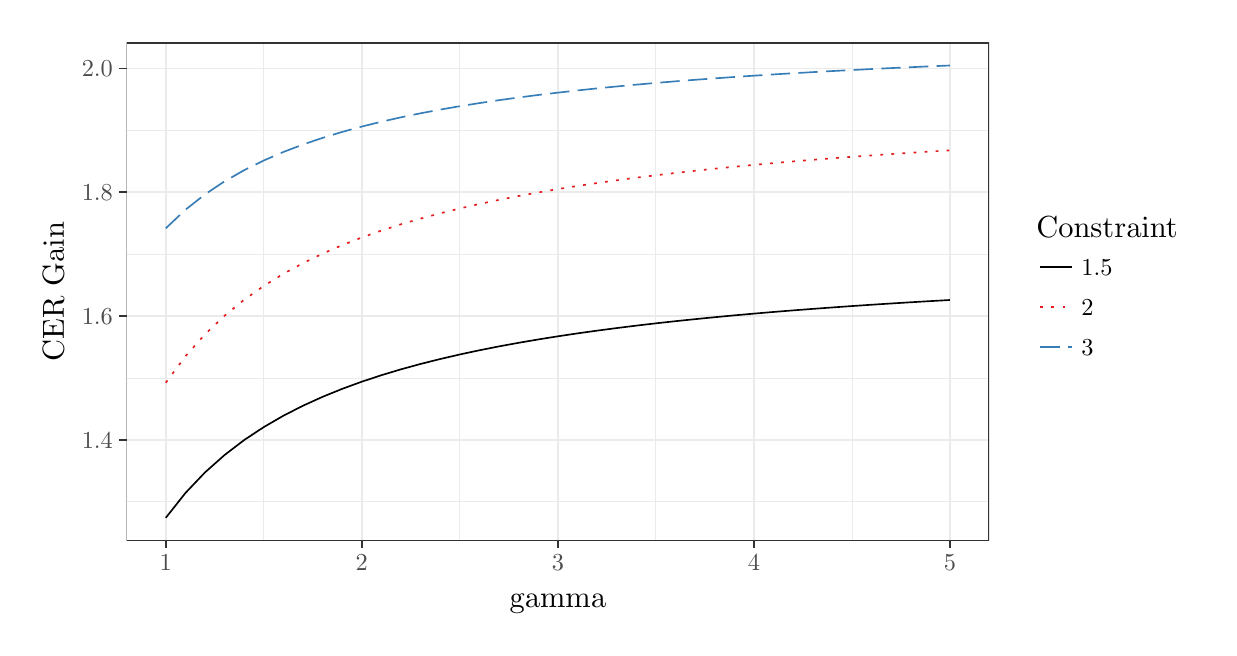
\begin{tikzpicture}[x=1pt,y=1pt]
\definecolor{fillColor}{RGB}{255,255,255}
\path[use as bounding box,fill=fillColor,fill opacity=0.00] (0,0) rectangle (426.79,216.81);
\begin{scope}
\path[clip] (  0.00,  0.00) rectangle (426.79,216.81);
\definecolor{drawColor}{RGB}{255,255,255}
\definecolor{fillColor}{RGB}{255,255,255}

\path[draw=drawColor,line width= 0.6pt,line join=round,line cap=round,fill=fillColor] (  0.00,  0.00) rectangle (426.79,216.81);
\end{scope}
\begin{scope}
\path[clip] ( 35.74, 31.53) rectangle (347.42,211.31);
\definecolor{fillColor}{RGB}{255,255,255}

\path[fill=fillColor] ( 35.74, 31.53) rectangle (347.42,211.31);
\definecolor{drawColor}{gray}{0.92}

\path[draw=drawColor,line width= 0.3pt,line join=round] ( 35.74, 45.51) --
	(347.42, 45.51);

\path[draw=drawColor,line width= 0.3pt,line join=round] ( 35.74, 90.23) --
	(347.42, 90.23);

\path[draw=drawColor,line width= 0.3pt,line join=round] ( 35.74,134.95) --
	(347.42,134.95);

\path[draw=drawColor,line width= 0.3pt,line join=round] ( 35.74,179.67) --
	(347.42,179.67);

\path[draw=drawColor,line width= 0.3pt,line join=round] ( 85.33, 31.53) --
	( 85.33,211.31);

\path[draw=drawColor,line width= 0.3pt,line join=round] (156.16, 31.53) --
	(156.16,211.31);

\path[draw=drawColor,line width= 0.3pt,line join=round] (227.00, 31.53) --
	(227.00,211.31);

\path[draw=drawColor,line width= 0.3pt,line join=round] (297.84, 31.53) --
	(297.84,211.31);

\path[draw=drawColor,line width= 0.6pt,line join=round] ( 35.74, 67.87) --
	(347.42, 67.87);

\path[draw=drawColor,line width= 0.6pt,line join=round] ( 35.74,112.59) --
	(347.42,112.59);

\path[draw=drawColor,line width= 0.6pt,line join=round] ( 35.74,157.31) --
	(347.42,157.31);

\path[draw=drawColor,line width= 0.6pt,line join=round] ( 35.74,202.03) --
	(347.42,202.03);

\path[draw=drawColor,line width= 0.6pt,line join=round] ( 49.91, 31.53) --
	( 49.91,211.31);

\path[draw=drawColor,line width= 0.6pt,line join=round] (120.74, 31.53) --
	(120.74,211.31);

\path[draw=drawColor,line width= 0.6pt,line join=round] (191.58, 31.53) --
	(191.58,211.31);

\path[draw=drawColor,line width= 0.6pt,line join=round] (262.42, 31.53) --
	(262.42,211.31);

\path[draw=drawColor,line width= 0.6pt,line join=round] (333.25, 31.53) --
	(333.25,211.31);
\definecolor{drawColor}{RGB}{0,0,0}

\path[draw=drawColor,line width= 0.6pt,line join=round] ( 49.91, 39.70) --
	( 56.99, 48.65) --
	( 64.07, 56.10) --
	( 71.16, 62.40) --
	( 78.24, 67.81) --
	( 85.33, 72.49) --
	( 92.41, 76.59) --
	( 99.49, 80.21) --
	(106.58, 83.42) --
	(113.66, 86.30) --
	(120.74, 88.89) --
	(127.83, 91.23) --
	(134.91, 93.36) --
	(141.99, 95.30) --
	(149.08, 97.08) --
	(156.16, 98.72) --
	(163.25,100.24) --
	(170.33,101.64) --
	(177.41,102.94) --
	(184.50,104.15) --
	(191.58,105.28) --
	(198.66,106.34) --
	(205.75,107.33) --
	(212.83,108.26) --
	(219.92,109.14) --
	(227.00,109.97) --
	(234.08,110.75) --
	(241.17,111.48) --
	(248.25,112.18) --
	(255.33,112.85) --
	(262.42,113.48) --
	(269.50,114.08) --
	(276.58,114.65) --
	(283.67,115.19) --
	(290.75,115.71) --
	(297.84,116.21) --
	(304.92,116.69) --
	(312.00,117.14) --
	(319.09,117.58) --
	(326.17,118.00) --
	(333.25,118.40);
\definecolor{drawColor}{RGB}{228,26,28}

\path[draw=drawColor,line width= 0.6pt,dash pattern=on 1pt off 3pt ,line join=round] ( 49.91, 88.51) --
	( 56.99, 98.05) --
	( 64.07,106.00) --
	( 71.16,112.73) --
	( 78.24,118.50) --
	( 85.33,123.49) --
	( 92.41,127.87) --
	( 99.49,131.73) --
	(106.58,135.16) --
	(113.66,138.23) --
	(120.74,140.99) --
	(127.83,143.49) --
	(134.91,145.76) --
	(141.99,147.83) --
	(149.08,149.73) --
	(156.16,151.48) --
	(163.25,153.10) --
	(170.33,154.59) --
	(177.41,155.98) --
	(184.50,157.27) --
	(191.58,158.48) --
	(198.66,159.61) --
	(205.75,160.67) --
	(212.83,161.66) --
	(219.92,162.60) --
	(227.00,163.48) --
	(234.08,164.31) --
	(241.17,165.10) --
	(248.25,165.85) --
	(255.33,166.55) --
	(262.42,167.23) --
	(269.50,167.87) --
	(276.58,168.48) --
	(283.67,169.06) --
	(290.75,169.61) --
	(297.84,170.14) --
	(304.92,170.65) --
	(312.00,171.14) --
	(319.09,171.60) --
	(326.17,172.05) --
	(333.25,172.48);
\definecolor{drawColor}{RGB}{55,126,184}

\path[draw=drawColor,line width= 0.6pt,dash pattern=on 7pt off 3pt ,line join=round] ( 49.91,144.31) --
	( 56.99,151.00) --
	( 64.07,156.57) --
	( 71.16,161.28) --
	( 78.24,165.32) --
	( 85.33,168.82) --
	( 92.41,171.89) --
	( 99.49,174.59) --
	(106.58,176.99) --
	(113.66,179.14) --
	(120.74,181.08) --
	(127.83,182.83) --
	(134.91,184.42) --
	(141.99,185.87) --
	(149.08,187.21) --
	(156.16,188.43) --
	(163.25,189.56) --
	(170.33,190.61) --
	(177.41,191.58) --
	(184.50,192.49) --
	(191.58,193.33) --
	(198.66,194.12) --
	(205.75,194.87) --
	(212.83,195.56) --
	(219.92,196.22) --
	(227.00,196.84) --
	(234.08,197.42) --
	(241.17,197.97) --
	(248.25,198.49) --
	(255.33,198.99) --
	(262.42,199.46) --
	(269.50,199.91) --
	(276.58,200.34) --
	(283.67,200.74) --
	(290.75,201.13) --
	(297.84,201.50) --
	(304.92,201.86) --
	(312.00,202.20) --
	(319.09,202.53) --
	(326.17,202.84) --
	(333.25,203.14);
\definecolor{drawColor}{gray}{0.20}

\path[draw=drawColor,line width= 0.6pt,line join=round,line cap=round] ( 35.74, 31.53) rectangle (347.42,211.31);
\end{scope}
\begin{scope}
\path[clip] (  0.00,  0.00) rectangle (426.79,216.81);
\definecolor{drawColor}{gray}{0.30}

\node[text=drawColor,anchor=base east,inner sep=0pt, outer sep=0pt, scale=  0.88] at ( 30.79, 64.84) {1.4};

\node[text=drawColor,anchor=base east,inner sep=0pt, outer sep=0pt, scale=  0.88] at ( 30.79,109.56) {1.6};

\node[text=drawColor,anchor=base east,inner sep=0pt, outer sep=0pt, scale=  0.88] at ( 30.79,154.28) {1.8};

\node[text=drawColor,anchor=base east,inner sep=0pt, outer sep=0pt, scale=  0.88] at ( 30.79,199.00) {2.0};
\end{scope}
\begin{scope}
\path[clip] (  0.00,  0.00) rectangle (426.79,216.81);
\definecolor{drawColor}{gray}{0.20}

\path[draw=drawColor,line width= 0.6pt,line join=round] ( 32.99, 67.87) --
	( 35.74, 67.87);

\path[draw=drawColor,line width= 0.6pt,line join=round] ( 32.99,112.59) --
	( 35.74,112.59);

\path[draw=drawColor,line width= 0.6pt,line join=round] ( 32.99,157.31) --
	( 35.74,157.31);

\path[draw=drawColor,line width= 0.6pt,line join=round] ( 32.99,202.03) --
	( 35.74,202.03);
\end{scope}
\begin{scope}
\path[clip] (  0.00,  0.00) rectangle (426.79,216.81);
\definecolor{drawColor}{gray}{0.20}

\path[draw=drawColor,line width= 0.6pt,line join=round] ( 49.91, 28.78) --
	( 49.91, 31.53);

\path[draw=drawColor,line width= 0.6pt,line join=round] (120.74, 28.78) --
	(120.74, 31.53);

\path[draw=drawColor,line width= 0.6pt,line join=round] (191.58, 28.78) --
	(191.58, 31.53);

\path[draw=drawColor,line width= 0.6pt,line join=round] (262.42, 28.78) --
	(262.42, 31.53);

\path[draw=drawColor,line width= 0.6pt,line join=round] (333.25, 28.78) --
	(333.25, 31.53);
\end{scope}
\begin{scope}
\path[clip] (  0.00,  0.00) rectangle (426.79,216.81);
\definecolor{drawColor}{gray}{0.30}

\node[text=drawColor,anchor=base,inner sep=0pt, outer sep=0pt, scale=  0.88] at ( 49.91, 20.52) {1};

\node[text=drawColor,anchor=base,inner sep=0pt, outer sep=0pt, scale=  0.88] at (120.74, 20.52) {2};

\node[text=drawColor,anchor=base,inner sep=0pt, outer sep=0pt, scale=  0.88] at (191.58, 20.52) {3};

\node[text=drawColor,anchor=base,inner sep=0pt, outer sep=0pt, scale=  0.88] at (262.42, 20.52) {4};

\node[text=drawColor,anchor=base,inner sep=0pt, outer sep=0pt, scale=  0.88] at (333.25, 20.52) {5};
\end{scope}
\begin{scope}
\path[clip] (  0.00,  0.00) rectangle (426.79,216.81);
\definecolor{drawColor}{RGB}{0,0,0}

\node[text=drawColor,anchor=base,inner sep=0pt, outer sep=0pt, scale=  1.10] at (191.58,  7.44) {gamma};
\end{scope}
\begin{scope}
\path[clip] (  0.00,  0.00) rectangle (426.79,216.81);
\definecolor{drawColor}{RGB}{0,0,0}

\node[text=drawColor,rotate= 90.00,anchor=base,inner sep=0pt, outer sep=0pt, scale=  1.10] at ( 13.08,121.42) {CER Gain};
\end{scope}
\begin{scope}
\path[clip] (  0.00,  0.00) rectangle (426.79,216.81);
\definecolor{fillColor}{RGB}{255,255,255}

\path[fill=fillColor] (358.80, 88.45) rectangle (421.29,154.39);
\end{scope}
\begin{scope}
\path[clip] (  0.00,  0.00) rectangle (426.79,216.81);
\definecolor{drawColor}{RGB}{0,0,0}

\node[text=drawColor,anchor=base west,inner sep=0pt, outer sep=0pt, scale=  1.10] at (364.49,141.12) {Constraint};
\end{scope}
\begin{scope}
\path[clip] (  0.00,  0.00) rectangle (426.79,216.81);
\definecolor{fillColor}{RGB}{255,255,255}

\path[fill=fillColor] (364.49,123.05) rectangle (378.95,137.51);
\end{scope}
\begin{scope}
\path[clip] (  0.00,  0.00) rectangle (426.79,216.81);
\definecolor{drawColor}{RGB}{0,0,0}

\path[draw=drawColor,line width= 0.6pt,line join=round] (365.94,130.28) -- (377.50,130.28);
\end{scope}
\begin{scope}
\path[clip] (  0.00,  0.00) rectangle (426.79,216.81);
\definecolor{fillColor}{RGB}{255,255,255}

\path[fill=fillColor] (364.49,108.60) rectangle (378.95,123.05);
\end{scope}
\begin{scope}
\path[clip] (  0.00,  0.00) rectangle (426.79,216.81);
\definecolor{drawColor}{RGB}{228,26,28}

\path[draw=drawColor,line width= 0.6pt,dash pattern=on 1pt off 3pt ,line join=round] (365.94,115.83) -- (377.50,115.83);
\end{scope}
\begin{scope}
\path[clip] (  0.00,  0.00) rectangle (426.79,216.81);
\definecolor{fillColor}{RGB}{255,255,255}

\path[fill=fillColor] (364.49, 94.14) rectangle (378.95,108.60);
\end{scope}
\begin{scope}
\path[clip] (  0.00,  0.00) rectangle (426.79,216.81);
\definecolor{drawColor}{RGB}{55,126,184}

\path[draw=drawColor,line width= 0.6pt,dash pattern=on 7pt off 3pt ,line join=round] (365.94,101.37) -- (377.50,101.37);
\end{scope}
\begin{scope}
\path[clip] (  0.00,  0.00) rectangle (426.79,216.81);
\definecolor{drawColor}{RGB}{0,0,0}

\node[text=drawColor,anchor=base west,inner sep=0pt, outer sep=0pt, scale=  0.88] at (380.75,127.25) {1.5};
\end{scope}
\begin{scope}
\path[clip] (  0.00,  0.00) rectangle (426.79,216.81);
\definecolor{drawColor}{RGB}{0,0,0}

\node[text=drawColor,anchor=base west,inner sep=0pt, outer sep=0pt, scale=  0.88] at (380.75,112.80) {2};
\end{scope}
\begin{scope}
\path[clip] (  0.00,  0.00) rectangle (426.79,216.81);
\definecolor{drawColor}{RGB}{0,0,0}

\node[text=drawColor,anchor=base west,inner sep=0pt, outer sep=0pt, scale=  0.88] at (380.75, 98.34) {3};
\end{scope}
\end{tikzpicture}

	\end{adjustbox}
\end{frame}

\begin{frame}{Leverage}
	\begin{adjustbox}{width=\textwidth}
		% Created by tikzDevice version 0.10.1 on 2018-06-14 11:50:00
% !TEX encoding = UTF-8 Unicode
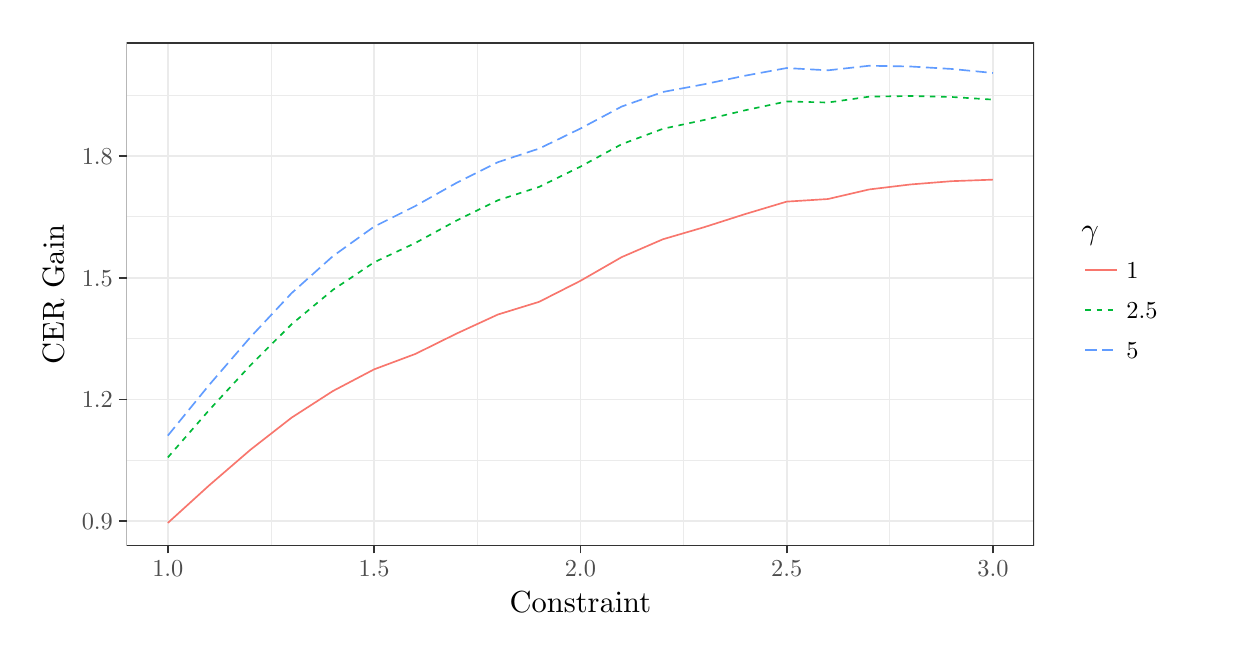
\begin{tikzpicture}[x=1pt,y=1pt]
\definecolor{fillColor}{RGB}{255,255,255}
\path[use as bounding box,fill=fillColor,fill opacity=0.00] (0,0) rectangle (426.79,216.81);
\begin{scope}
\path[clip] (  0.00,  0.00) rectangle (426.79,216.81);
\definecolor{drawColor}{RGB}{255,255,255}
\definecolor{fillColor}{RGB}{255,255,255}

\path[draw=drawColor,line width= 0.6pt,line join=round,line cap=round,fill=fillColor] (  0.00,  0.00) rectangle (426.79,216.81);
\end{scope}
\begin{scope}
\path[clip] ( 35.74, 29.59) rectangle (363.70,211.31);
\definecolor{fillColor}{RGB}{255,255,255}

\path[fill=fillColor] ( 35.74, 29.59) rectangle (363.70,211.31);
\definecolor{drawColor}{gray}{0.92}

\path[draw=drawColor,line width= 0.3pt,line join=round] ( 35.74, 60.51) --
	(363.70, 60.51);

\path[draw=drawColor,line width= 0.3pt,line join=round] ( 35.74,104.47) --
	(363.70,104.47);

\path[draw=drawColor,line width= 0.3pt,line join=round] ( 35.74,148.43) --
	(363.70,148.43);

\path[draw=drawColor,line width= 0.3pt,line join=round] ( 35.74,192.39) --
	(363.70,192.39);

\path[draw=drawColor,line width= 0.3pt,line join=round] ( 87.92, 29.59) --
	( 87.92,211.31);

\path[draw=drawColor,line width= 0.3pt,line join=round] (162.45, 29.59) --
	(162.45,211.31);

\path[draw=drawColor,line width= 0.3pt,line join=round] (236.99, 29.59) --
	(236.99,211.31);

\path[draw=drawColor,line width= 0.3pt,line join=round] (311.53, 29.59) --
	(311.53,211.31);

\path[draw=drawColor,line width= 0.6pt,line join=round] ( 35.74, 38.53) --
	(363.70, 38.53);

\path[draw=drawColor,line width= 0.6pt,line join=round] ( 35.74, 82.49) --
	(363.70, 82.49);

\path[draw=drawColor,line width= 0.6pt,line join=round] ( 35.74,126.45) --
	(363.70,126.45);

\path[draw=drawColor,line width= 0.6pt,line join=round] ( 35.74,170.41) --
	(363.70,170.41);

\path[draw=drawColor,line width= 0.6pt,line join=round] ( 50.65, 29.59) --
	( 50.65,211.31);

\path[draw=drawColor,line width= 0.6pt,line join=round] (125.18, 29.59) --
	(125.18,211.31);

\path[draw=drawColor,line width= 0.6pt,line join=round] (199.72, 29.59) --
	(199.72,211.31);

\path[draw=drawColor,line width= 0.6pt,line join=round] (274.26, 29.59) --
	(274.26,211.31);

\path[draw=drawColor,line width= 0.6pt,line join=round] (348.80, 29.59) --
	(348.80,211.31);
\definecolor{drawColor}{RGB}{248,118,109}

\path[draw=drawColor,line width= 0.6pt,line join=round] ( 50.65, 37.85) --
	( 65.55, 51.39) --
	( 80.46, 64.26) --
	( 95.37, 75.89) --
	(110.28, 85.50) --
	(125.18, 93.34) --
	(140.09, 98.91) --
	(155.00,106.28) --
	(169.91,113.15) --
	(184.81,117.74) --
	(199.72,125.32) --
	(214.63,133.89) --
	(229.54,140.35) --
	(244.44,144.71) --
	(259.35,149.48) --
	(274.26,153.95) --
	(289.17,154.89) --
	(304.07,158.35) --
	(318.98,160.15) --
	(333.89,161.34) --
	(348.80,161.89);
\definecolor{drawColor}{RGB}{0,186,56}

\path[draw=drawColor,line width= 0.6pt,dash pattern=on 2pt off 2pt ,line join=round] ( 50.65, 61.51) --
	( 65.55, 78.60) --
	( 80.46, 94.77) --
	( 95.37,109.64) --
	(110.28,122.05) --
	(125.18,132.02) --
	(140.09,139.01) --
	(155.00,147.13) --
	(169.91,154.44) --
	(184.81,159.27) --
	(199.72,166.59) --
	(214.63,174.70) --
	(229.54,180.27) --
	(244.44,183.45) --
	(259.35,186.98) --
	(274.26,190.15) --
	(289.17,189.76) --
	(304.07,191.88) --
	(318.98,192.12) --
	(333.89,191.76) --
	(348.80,190.81);
\definecolor{drawColor}{RGB}{97,156,255}

\path[draw=drawColor,line width= 0.6pt,dash pattern=on 4pt off 2pt ,line join=round] ( 50.65, 69.40) --
	( 65.55, 87.67) --
	( 80.46,104.94) --
	( 95.37,120.88) --
	(110.28,134.24) --
	(125.18,144.91) --
	(140.09,152.37) --
	(155.00,160.75) --
	(169.91,168.21) --
	(184.81,173.11) --
	(199.72,180.35) --
	(214.63,188.30) --
	(229.54,193.57) --
	(244.44,196.36) --
	(259.35,199.48) --
	(274.26,202.22) --
	(289.17,201.39) --
	(304.07,203.05) --
	(318.98,202.78) --
	(333.89,201.89) --
	(348.80,200.44);
\definecolor{drawColor}{gray}{0.20}

\path[draw=drawColor,line width= 0.6pt,line join=round,line cap=round] ( 35.74, 29.59) rectangle (363.70,211.31);
\end{scope}
\begin{scope}
\path[clip] (  0.00,  0.00) rectangle (426.79,216.81);
\definecolor{drawColor}{gray}{0.30}

\node[text=drawColor,anchor=base east,inner sep=0pt, outer sep=0pt, scale=  0.88] at ( 30.79, 35.50) {0.9};

\node[text=drawColor,anchor=base east,inner sep=0pt, outer sep=0pt, scale=  0.88] at ( 30.79, 79.46) {1.2};

\node[text=drawColor,anchor=base east,inner sep=0pt, outer sep=0pt, scale=  0.88] at ( 30.79,123.42) {1.5};

\node[text=drawColor,anchor=base east,inner sep=0pt, outer sep=0pt, scale=  0.88] at ( 30.79,167.38) {1.8};
\end{scope}
\begin{scope}
\path[clip] (  0.00,  0.00) rectangle (426.79,216.81);
\definecolor{drawColor}{gray}{0.20}

\path[draw=drawColor,line width= 0.6pt,line join=round] ( 32.99, 38.53) --
	( 35.74, 38.53);

\path[draw=drawColor,line width= 0.6pt,line join=round] ( 32.99, 82.49) --
	( 35.74, 82.49);

\path[draw=drawColor,line width= 0.6pt,line join=round] ( 32.99,126.45) --
	( 35.74,126.45);

\path[draw=drawColor,line width= 0.6pt,line join=round] ( 32.99,170.41) --
	( 35.74,170.41);
\end{scope}
\begin{scope}
\path[clip] (  0.00,  0.00) rectangle (426.79,216.81);
\definecolor{drawColor}{gray}{0.20}

\path[draw=drawColor,line width= 0.6pt,line join=round] ( 50.65, 26.84) --
	( 50.65, 29.59);

\path[draw=drawColor,line width= 0.6pt,line join=round] (125.18, 26.84) --
	(125.18, 29.59);

\path[draw=drawColor,line width= 0.6pt,line join=round] (199.72, 26.84) --
	(199.72, 29.59);

\path[draw=drawColor,line width= 0.6pt,line join=round] (274.26, 26.84) --
	(274.26, 29.59);

\path[draw=drawColor,line width= 0.6pt,line join=round] (348.80, 26.84) --
	(348.80, 29.59);
\end{scope}
\begin{scope}
\path[clip] (  0.00,  0.00) rectangle (426.79,216.81);
\definecolor{drawColor}{gray}{0.30}

\node[text=drawColor,anchor=base,inner sep=0pt, outer sep=0pt, scale=  0.88] at ( 50.65, 18.58) {1.0};

\node[text=drawColor,anchor=base,inner sep=0pt, outer sep=0pt, scale=  0.88] at (125.18, 18.58) {1.5};

\node[text=drawColor,anchor=base,inner sep=0pt, outer sep=0pt, scale=  0.88] at (199.72, 18.58) {2.0};

\node[text=drawColor,anchor=base,inner sep=0pt, outer sep=0pt, scale=  0.88] at (274.26, 18.58) {2.5};

\node[text=drawColor,anchor=base,inner sep=0pt, outer sep=0pt, scale=  0.88] at (348.80, 18.58) {3.0};
\end{scope}
\begin{scope}
\path[clip] (  0.00,  0.00) rectangle (426.79,216.81);
\definecolor{drawColor}{RGB}{0,0,0}

\node[text=drawColor,anchor=base,inner sep=0pt, outer sep=0pt, scale=  1.10] at (199.72,  5.50) {Constraint};
\end{scope}
\begin{scope}
\path[clip] (  0.00,  0.00) rectangle (426.79,216.81);
\definecolor{drawColor}{RGB}{0,0,0}

\node[text=drawColor,rotate= 90.00,anchor=base,inner sep=0pt, outer sep=0pt, scale=  1.10] at ( 13.08,120.45) {CER Gain};
\end{scope}
\begin{scope}
\path[clip] (  0.00,  0.00) rectangle (426.79,216.81);
\definecolor{fillColor}{RGB}{255,255,255}

\path[fill=fillColor] (375.09, 87.48) rectangle (421.29,153.41);
\end{scope}
\begin{scope}
\path[clip] (  0.00,  0.00) rectangle (426.79,216.81);
\definecolor{drawColor}{RGB}{0,0,0}

\node[text=drawColor,anchor=base west,inner sep=0pt, outer sep=0pt, scale=  1.10] at (380.78,140.15) {$\gamma$};
\end{scope}
\begin{scope}
\path[clip] (  0.00,  0.00) rectangle (426.79,216.81);
\definecolor{fillColor}{RGB}{255,255,255}

\path[fill=fillColor] (380.78,122.08) rectangle (395.23,136.53);
\end{scope}
\begin{scope}
\path[clip] (  0.00,  0.00) rectangle (426.79,216.81);
\definecolor{drawColor}{RGB}{248,118,109}

\path[draw=drawColor,line width= 0.6pt,line join=round] (382.22,129.31) -- (393.78,129.31);
\end{scope}
\begin{scope}
\path[clip] (  0.00,  0.00) rectangle (426.79,216.81);
\definecolor{fillColor}{RGB}{255,255,255}

\path[fill=fillColor] (380.78,107.63) rectangle (395.23,122.08);
\end{scope}
\begin{scope}
\path[clip] (  0.00,  0.00) rectangle (426.79,216.81);
\definecolor{drawColor}{RGB}{0,186,56}

\path[draw=drawColor,line width= 0.6pt,dash pattern=on 2pt off 2pt ,line join=round] (382.22,114.85) -- (393.78,114.85);
\end{scope}
\begin{scope}
\path[clip] (  0.00,  0.00) rectangle (426.79,216.81);
\definecolor{fillColor}{RGB}{255,255,255}

\path[fill=fillColor] (380.78, 93.17) rectangle (395.23,107.63);
\end{scope}
\begin{scope}
\path[clip] (  0.00,  0.00) rectangle (426.79,216.81);
\definecolor{drawColor}{RGB}{97,156,255}

\path[draw=drawColor,line width= 0.6pt,dash pattern=on 4pt off 2pt ,line join=round] (382.22,100.40) -- (393.78,100.40);
\end{scope}
\begin{scope}
\path[clip] (  0.00,  0.00) rectangle (426.79,216.81);
\definecolor{drawColor}{RGB}{0,0,0}

\node[text=drawColor,anchor=base west,inner sep=0pt, outer sep=0pt, scale=  0.88] at (397.04,126.28) {1};
\end{scope}
\begin{scope}
\path[clip] (  0.00,  0.00) rectangle (426.79,216.81);
\definecolor{drawColor}{RGB}{0,0,0}

\node[text=drawColor,anchor=base west,inner sep=0pt, outer sep=0pt, scale=  0.88] at (397.04,111.82) {2.5};
\end{scope}
\begin{scope}
\path[clip] (  0.00,  0.00) rectangle (426.79,216.81);
\definecolor{drawColor}{RGB}{0,0,0}

\node[text=drawColor,anchor=base west,inner sep=0pt, outer sep=0pt, scale=  0.88] at (397.04, 97.37) {5};
\end{scope}
\end{tikzpicture}

	\end{adjustbox}
	Risk averse, mean-variance investors see substantial utility gains switching from the SV to AV managed portfolio and these gains increase with leverage usage and risk aversion
\end{frame}

%\subsection{In Sample}
%%\item $W_{t}$ = $\frac{1}{AV_{t-1}}$ is the investment weight on the CRSP market portfolio
%\begin{frame}{Variance Prediction}
%	\vspace{-6pt}
%	\begin{center}
%		1926:08-2016:12
%	\end{center}
%		\vspace{-30pt}
% \begin{table}
% 	\begin{adjustbox}{width=\textwidth,height=3.5cm}
% 	
% Table created by stargazer v.5.2 by Marek Hlavac, Harvard University. E-mail: hlavac at fas.harvard.edu
% Date and time: Fri, Jun 08, 2018 - 12:52:08  IST
\begin{tabular}{@{\extracolsep{5pt}}lccccc} 
\\[-1.8ex]
\hline \\[-1.8ex] 
AV & 0.627$^{***}$ &  &  & 0.553$^{***}$ & 0.368$^{***}$ \\ 
& p = 0.000 &  &  & p = 0.000 & p = 0.000 \\ 
%& & & & & \\ 
AC &  & 0.418$^{***}$ &  & 0.160$^{***}$ &  \\ 
&  & p = 0.000 &  & p = 0.000 &  \\ 
%& & & & & \\ 
SV &  &  & 0.615$^{***}$ &  & 0.278$^{***}$ \\ 
&  &  & p = 0.000 &  & p = 0.000 \\ 
%& & & & & \\ 
Constant & $-$0.0003 & $-$0.0001 & $-$0.0002 & $-$0.0003 & $-$0.0003 \\ 
& p = 0.991 & p = 0.998 & p = 0.993 & p = 0.991 & p = 0.991 \\ 
%& & & & & \\ 
%\textit{N} & 1,085 & 1,085 & 1,085 & 1,085 & 1,085 \\ 
R$^{2}$ & 0.391 & 0.173 & 0.375 & 0.410 & 0.413 \\ 
Adjusted R$^{2}$ & 0.390 & 0.173 & 0.374 & 0.409 & 0.412 \\ 
%\hline 
\hline \\[-1.8ex] 
%\textit{Notes:} & \multicolumn{5}{r}{$^{***}$Significant at the 1 percent level.} \\ 
% & \multicolumn{5}{r}{$^{**}$Significant at the 5 percent level.} \\ 
% & \multicolumn{5}{r}{$^{*}$Significant at the 10 percent level.} \\ 
\end{tabular} 

% 	\end{adjustbox}
%
% \end{table}
%\end{frame}

%\begin{frame}{AV Prediction}
%	\vspace{-12pt}
%	\begin{table}
%		\begin{adjustbox}{width=\textwidth,height=4cm}
%			
% Table created by stargazer v.5.2 by Marek Hlavac, Harvard University. E-mail: hlavac at fas.harvard.edu
% Date and time: Fri, Mar 30, 2018 - 02:49:44  IST
\begin{table}[!htbp] \centering 
  \caption{} 
  \label{} 
\begin{tabular}{@{\extracolsep{5pt}}lccccc} 
\\[-1.8ex]\hline 
\hline \\[-1.8ex] 
 & \multicolumn{5}{c}{\textit{Dependent variable:}} \\ 
\cline{2-6} 
\\[-1.8ex] & \multicolumn{5}{c}{AV$_{t+1}$} \\ 
\\[-1.8ex] & (1) & (2) & (3) & (4) & (5)\\ 
\hline \\[-1.8ex] 
 AC$_{t}$ & 0.014$^{***}$ &  &  & $-$0.001 &  \\ 
  & (0.003) &  &  & (0.002) &  \\ 
  & & & & & \\ 
 AV$_{t}$ &  & 0.667$^{***}$ &  & 0.674$^{***}$ & 1.030$^{***}$ \\ 
  &  & (0.029) &  & (0.031) & (0.065) \\ 
  & & & & & \\ 
 SV$_{t}$ &  &  & 1.092$^{***}$ &  & $-$0.844$^{***}$ \\ 
  &  &  & (0.070) &  & (0.135) \\ 
  & & & & & \\ 
 Constant & 0.004$^{***}$ & 0.003$^{***}$ & 0.006$^{***}$ & 0.003$^{***}$ & 0.001$^{***}$ \\ 
  & (0.001) & (0.0003) & (0.0003) & (0.001) & (0.0004) \\ 
  & & & & & \\ 
\hline \\[-1.8ex] 
Observations & 654 & 654 & 654 & 654 & 654 \\ 
R$^{2}$ & 0.048 & 0.445 & 0.273 & 0.446 & 0.477 \\ 
Adjusted R$^{2}$ & 0.046 & 0.445 & 0.272 & 0.444 & 0.475 \\ 
Residual Std. Error & 0.008 (df = 652) & 0.006 (df = 652) & 0.007 (df = 652) & 0.006 (df = 651) & 0.006 (df = 651) \\ 
F Statistic & 32.601$^{***}$ (df = 1; 652) & 523.763$^{***}$ (df = 1; 652) & 244.654$^{***}$ (df = 1; 652) & 261.813$^{***}$ (df = 2; 651) & 296.603$^{***}$ (df = 2; 651) \\ 
\hline 
\hline \\[-1.8ex] 
\textit{Note:}  & \multicolumn{5}{r}{$^{*}$p$<$0.1; $^{**}$p$<$0.05; $^{***}$p$<$0.01} \\ 
\end{tabular} 
\end{table} 

%		\end{adjustbox}
%		
%	\end{table}
%\end{frame}

%\begin{frame}{Return Prediction}
%		\vspace{-6pt}
%		\begin{center}
%			1926:08-2016:12
%		\end{center}
%		\vspace{-30pt}
%	\begin{table}
%		\begin{adjustbox}{width=\textwidth,height=3.5cm}
%			
% Table created by stargazer v.5.2 by Marek Hlavac, Harvard University. E-mail: hlavac at fas.harvard.edu
% Date and time: Thu, Apr 05, 2018 - 02:24:48  IST
\begin{tabular}{@{\extracolsep{5pt}}lccccc} 
\\[-1.8ex]\hline 
\hline \\[-1.8ex] 
\\[-1.8ex] & \multicolumn{5}{c}{RET$_{t+1}$} \\ 
\hline \\[-1.8ex] 
 AV & 0.001 &  &  & $-$0.026 & 0.764$^{***}$ \\ 
  & p = 0.996 &  &  & p = 0.857 & p = 0.002 \\ 
  & & & & & \\ 
 AC &  & 0.004 &  & 0.005 &  \\ 
  &  & p = 0.724 &  & p = 0.692 &  \\ 
  & & & & & \\ 
 SV &  &  & $-$0.604$^{*}$ &  & $-$2.275$^{***}$ \\ 
  &  &  & p = 0.064 &  & p = 0.0003 \\ 
  & & & & & \\ 
 Constant & 0.005$^{**}$ & 0.004 & 0.006$^{***}$ & 0.004 & 0.004$^{*}$ \\ 
  & p = 0.013 & p = 0.315 & p = 0.0005 & p = 0.331 & p = 0.054 \\ 
  & & & & & \\ 
\textit{N} & 1,085 & 1,085 & 1,085 & 1,085 & 1,085 \\ 
R$^{2}$ & 0.00000 & 0.0001 & 0.003 & 0.0001 & 0.012 \\ 
Adjusted R$^{2}$ & $-$0.001 & $-$0.001 & 0.002 & $-$0.002 & 0.010 \\ 
\hline 
\hline \\[-1.8ex] 
\textit{Notes:} & \multicolumn{5}{r}{$^{***}$Significant at the 1 percent level.} \\ 
 & \multicolumn{5}{r}{$^{**}$Significant at the 5 percent level.} \\ 
 & \multicolumn{5}{r}{$^{*}$Significant at the 10 percent level.} \\ 
\end{tabular} 

%		\end{adjustbox}
%		
%	\end{table}
%\end{frame}

%\begin{frame}{Risk vs Return}
%	\vspace{-12pt}
%	\begin{table}
%		\caption{1962M7:2016M12}
%		\vspace{-6pt}
%		\begin{adjustbox}{width=10cm,height=4cm}
%			
% Table created by stargazer v.5.2 by Marek Hlavac, Harvard University. E-mail: hlavac at fas.harvard.edu
% Date and time: Mon, Mar 19, 2018 - 01:36:39  IST
\begin{table}[!htbp] \centering 
  \caption{} 
  \label{} 
\begin{tabular}{@{\extracolsep{5pt}}lcccccccccccc} 
\\[-1.8ex]\hline 
\hline \\[-1.8ex] 
 & \multicolumn{12}{c}{\textit{Dependent variable:}} \\ 
\cline{2-13} 
\\[-1.8ex] & \multicolumn{3}{c}{RET$_{t+1}$} & \multicolumn{3}{c}{RET$_{t+3}$} & \multicolumn{3}{c}{RET$_{t+6}$} & \multicolumn{3}{c}{RET$_{t+12}$} \\ 
\\[-1.8ex] & (1) & (2) & (3) & (4) & (5) & (6) & (7) & (8) & (9) & (10) & (11) & (12)\\ 
\hline \\[-1.8ex] 
 AV$_{t}$ & $-$0.688$^{***}$ &  & $-$0.880$^{*}$ & $-$0.958$^{**}$ &  & $-$2.959$^{***}$ & $-$0.751 &  & $-$6.371$^{***}$ & $-$0.921 &  & $-$11.702$^{***}$ \\ 
  & (0.204) &  & (0.469) & (0.371) &  & (0.848) & (0.542) &  & (1.220) & (0.764) &  & (1.692) \\ 
  & & & & & & & & & & & & \\ 
 SV$_{t}$ &  & $-$1.206$^{***}$ & 0.446 &  & $-$0.918 & 4.633$^{***}$ &  & 1.054 & 13.004$^{***}$ &  & 2.988$^{*}$ & 24.933$^{***}$ \\ 
  &  & (0.426) & (0.977) &  & (0.776) & (1.766) &  & (1.129) & (2.542) &  & (1.588) & (3.523) \\ 
  & & & & & & & & & & & & \\ 
 Constant & 0.009$^{***}$ & 0.006$^{***}$ & 0.010$^{***}$ & 0.019$^{***}$ & 0.014$^{***}$ & 0.025$^{***}$ & 0.029$^{***}$ & 0.021$^{***}$ & 0.047$^{***}$ & 0.053$^{***}$ & 0.040$^{***}$ & 0.086$^{***}$ \\ 
  & (0.002) & (0.002) & (0.003) & (0.004) & (0.004) & (0.005) & (0.006) & (0.005) & (0.007) & (0.009) & (0.007) & (0.010) \\ 
  & & & & & & & & & & & & \\ 
\hline \\[-1.8ex] 
Observations & 643 & 643 & 643 & 641 & 641 & 641 & 638 & 638 & 638 & 632 & 632 & 632 \\ 
R$^{2}$ & 0.017 & 0.012 & 0.018 & 0.010 & 0.002 & 0.021 & 0.003 & 0.001 & 0.042 & 0.002 & 0.006 & 0.076 \\ 
Adjusted R$^{2}$ & 0.016 & 0.011 & 0.015 & 0.009 & 0.001 & 0.018 & 0.001 & $-$0.0002 & 0.039 & 0.001 & 0.004 & 0.073 \\ 
Residual Std. Error & 0.044 (df = 641) & 0.044 (df = 641) & 0.044 (df = 640) & 0.080 (df = 639) & 0.080 (df = 639) & 0.080 (df = 638) & 0.117 (df = 636) & 0.117 (df = 636) & 0.115 (df = 635) & 0.165 (df = 630) & 0.164 (df = 630) & 0.159 (df = 629) \\ 
F Statistic & 11.365$^{***}$ (df = 1; 641) & 8.002$^{***}$ (df = 1; 641) & 5.779$^{***}$ (df = 2; 640) & 6.674$^{**}$ (df = 1; 639) & 1.402 (df = 1; 639) & 6.808$^{***}$ (df = 2; 638) & 1.926 (df = 1; 636) & 0.871 (df = 1; 636) & 14.085$^{***}$ (df = 2; 635) & 1.453 (df = 1; 630) & 3.542$^{*}$ (df = 1; 630) & 25.827$^{***}$ (df = 2; 629) \\ 
\hline 
\hline \\[-1.8ex] 
\textit{Note:}  & \multicolumn{12}{r}{$^{*}$p$<$0.1; $^{**}$p$<$0.05; $^{***}$p$<$0.01} \\ 
\end{tabular} 
\end{table} 

%		\end{adjustbox}
%	\end{table}
%\end{frame}

%\subsection{Out of Sample}
%\begin{frame}{Out-of-Sample Tests}
%	\begin{itemize}[<+->]
%		\item Divide the sample 1962:06 - 2016:12 into 15\% training 85\% prediction
%		\begin{itemize}
%			\item Initial training period $t = q$ months. First ~8 years.
%			\item Remaining period $t = q+1, q+2,..,T$ for out-of-sample forecast evaluation.
%		\end{itemize}
%		\item Regression model is "trained" over initial period
%		\begin{itemize}
%			\item Estimate $\hat \alpha_{t}$ and $\hat \beta_{t}$ by regressing $\{r_{s+1}\}_{s=1}^{t-1}$ on a constant and $\{x\}_{s=1}^{t-1}$
%		\end{itemize}
%		\item Generate one period ahead prediction \\
%		\begin{itemize}
%			\item $\hat r_{t+1} = \hat \alpha_{t} + \hat \beta_{t}x_{t}$
%		\end{itemize}
%		\item Each following month the ``training" window expands by one month
%	\end{itemize}
%\end{frame}
%

%
%\begin{frame}{Out of Sample Stats}
%	\begin{itemize}
%		\item $R_{oos}^{2}$ and MSE-F test improvement in forecast accuracy relative to a benchmark
%		\item Encompassing tests impose the greater requirement that the benchmark have no valuable forecasting information
%	\end{itemize}
%	\begin{block}{ENC-NEW Mcracken and Clark 2009}
%		\begin{itemize}
%			\item ENC-NEW = $T\times \frac{\frac{1}{T}\sum_{1}^{T}(e_{b,t}^{2}-e_{b,t}e_{x,t})}{MSFE_{x}}$
%			\item ENC-NEW = F-type statistic on the imporvement of including the benchmark
%		\end{itemize}
%	\end{block}
%	\begin{block}{ENC-HLN Harvey, Lebourne and Newbold 1998}
%		\begin{itemize}
%			\item Optimal forecast = $\hat{y}^{*}_{t} = (1-\lambda)\hat{y}_{b,t} + \lambda \hat{y}_{x,t}$
%			\item $\lambda$ = measure of the optimal combination of forecasts from x and the benchmark
%		\end{itemize}
%	\end{block}
%\end{frame}
%
%\begin{frame}{Out of Sample Results}
%	\vspace{-12pt}
%	\begin{table}
%		\caption{1970M7:2016M12}
%		\vspace{-6pt}
%		\begin{adjustbox}{width=\textwidth}
%			% Table created by stargazer v.5.2 by Marek Hlavac, Harvard University. E-mail: hlavac at fas.harvard.edu
% Date and time: Mon, Mar 26, 2018 - 07:05:02  IST
%\begin{table}[!htbp] \centering 
%	\caption{} 
%	\label{} 
	\begin{tabular}{@{\extracolsep{5pt}} cccccc} 
				\multicolumn{6}{c}{Benchmark: Historical Average}\\
		\\[-1.8ex]\hline 
		\hline \\[-1.8ex] 
		 & Sample & $R^{2}_{oos}$ & MSE-F & ENC-NEW & ENC-HLN \\ 
		\hline \\[-1.8ex] 
		%SV$_{t+1}$ & Monthly & 25.414* & $189.790$ & 160.994** & 1*** \\ 
		SV$_{t+1}$ & Monthly & 25.414* & $189.790$*** & 160.994** & 1*** \\ 
		%AV$_{t+1}$ & Monthly & 38.11** & $342.979$ & 355.228** & 0.967*** \\ 
		AV$_{t+1}$ & Monthly & 38.11** & $342.979$*** & 355.228** & 0.967*** \\ 
		%RET$_{t+3}$ & Monthly & 0.087 & $0.481$ & 4.917** & 0.526 \\ 
		RET$_{t+1}$ & Monthly & -0.059 & $$-$0.328$ & 3.493** & 0.478 \\ 
		%RET$_{t+3}$ & Monthly & 0.087 & $0.481$ & 4.917** & 0.526 \\ 
		\hline\\[-1.8ex]
		\multicolumn{6}{c}{Benchmark: SV$_{t}$}\\
			\\[-1.8ex]\hline 
			\hline \\[-1.8ex] 
			 & Sample & $R^{2}_{oos}$ & MSE-F & ENC-NEW & ENC-HLN \\ 
		SV$_{t+1}$ & Monthly & 4.041 & $23.454$*** & 25.409** & 0.929* \\ 
		%SV$_{t+1}$ & Monthly & 4.041 & $23.454$ & 25.409** & 0.929* \\ 
		%AV$_{t+1}$ & Monthly & 26.853 & $204.485$ & 135.494** & 1*** \\ 
		AV$_{t+1}$ & Monthly & 26.853 & $204.485$*** & 135.494** & 1*** \\ 
		%RET$_{t+3}$ & Monthly & 6.019 & $35.548$ & 30.218** & 1 \\ 
		RET$_{t+1}$ & Monthly & 2.116 & $12.043$*** & 8.2** & 1 \\ 
		%RET$_{t+3}$ & Monthly & 6.019 & $35.548$ & 30.218** & 1 \\ 
		\hline \\[-1.8ex] 
	\end{tabular} 
%\end{table} 
%		\end{adjustbox}
%	\end{table}
%\end{frame}

%\begin{frame}{Out of Sample Results}
%	\vspace{-12pt}
%	\begin{table}
%		\caption{Sample 1970:07 to 2016:12}
%		\vspace{-6pt}
%		\begin{adjustbox}{center,max height=\totalheight}
%			
% Table created by stargazer v.5.2 by Marek Hlavac, Harvard University. E-mail: hlavac at fas.harvard.edu
% Date and time: Sun, Jun 10, 2018 - 12:59:08  IST
\begin{tabular}{@{\extracolsep{5pt}} cccc} 
%\\[-1.8ex]\hline 
%\multicolumn{4}{c}{Benchmark - Hist Mean}\\
%\hline \\[-1.8ex] 

%\hline \\[-1.8ex] 
%AC$_{t+1}$ & -1.627 & -144.647 & 0 \\ 
%SV$_{t+1}$ & -1.631 & -27.854 & 0 \\ 
%AV$_{t+1}$ & -2.39 & -55.67 & 0 \\ 
%RET$_{t+1}$ & -0.238 & -1.533 & 0.265 \\ 
\\[-1.8ex]\hline 
%\multicolumn{4}{c}{Benchmark - SV$_{t}$}\\
 & DM & MSE-F & ENC-HLN \\ 
\hline \\[-1.8ex]
AC$_{t+1}$ & 1.074 & 109.736*** & 1 \\ 
SV$_{t+1}$ & 1.53* & 29.252*** & 1** \\ 
AV$_{t+1}$ & 2.286** & 109.333*** & 1*** \\ 
RET$_{t+1}$ & 1.278 & 11.801*** & 1* \\ 
\hline \\[-1.8ex] 
\end{tabular} 

%		\end{adjustbox}
%	\end{table}
%\end{frame}

%\begin{frame}{Out of Sample Results}
%	\vspace{-12pt}
%	\begin{table}
%		\caption{Sample 1939:12 to 2016:12}
%		\vspace{-6pt}
%		\begin{adjustbox}{center,max height=\totalheight}
%			
% Table created by stargazer v.5.2 by Marek Hlavac, Harvard University. E-mail: hlavac at fas.harvard.edu
% Date and time: Sun, Jun 10, 2018 - 12:56:34  IST
%\begin{table}[!htbp] \centering 
%  \caption{} 
%  \label{} 
\begin{tabular}{@{\extracolsep{5pt}} cccc} 
%\\[-1.8ex]\hline 
%\multicolumn{4}{c}{Benchmark - Hist Mean}\\
%\hline \\[-1.8ex] 

%\hline \\[-1.8ex] 
%AC$_{t+1}$ & -2.2 & -36.182 & 0.075 \\ 
%SV$_{t+1}$ & -0.431 & -8.453 & 0.403** \\ 
%AV$_{t+1}$ & -2.374 & -12.431 & 0 \\ 
%RET$_{t+1}$ & -1.766 & -4.832 & 0 \\ 
\hline \\[-1.8ex]
%\multicolumn{4}{c}{Benchmark - SV$_{t}$}\\
 & DM & MSE-F & ENC-HLN \\ 
\hline \\[-1.8ex]
AC$_{t+1}$ & 1.604* & 46.251*** & 1** \\ 
SV$_{t+1}$ & 1.041 & 21.57*** & 0.956** \\ 
AV$_{t+1}$ & 3.104*** & 198.267*** & 1*** \\ 
RET$_{t+1}$ & -2.027 & -8.702 & 0 \\ 
\hline \\[-1.8ex] 
%\textit{Notes:} & \multicolumn{3}{r}{$^{***}$,$^{**}$, and $^{*}$ Significant at the 1,} \\ 
%& \multicolumn{3}{r}{ 5, and 10 percent levels.}
\end{tabular} 
%\end{table} 

%		\end{adjustbox}
%	\end{table}
%\end{frame}



\section{Suggestively Systematic}

\subsection{Regression Subsamples}

\begin{frame}{AC/AV and Systematic Risk}
	\begin{itemize}[<+->]
		\item Pollet and Wilson (2010) - AC is positively related to the correlation of market returns and aggregate wealth, including the unobserved component of the "true market"
		\item AC signal changes in systematic risk when the daily returns used are a good proxy for the "true market" and the market is a significant part of aggregate wealth.
		\item This is similar to the difference in results between Goyal and Santa Clara (2003) and Bali et all (2005) when the latter removes a significant number of daily returns and the forecasting ability of idiosyncratic volatility disappears
		\item Thus we can run a placebo-like test on a sub-sample where the daily returns are not representative
	\end{itemize}
\end{frame}

\begin{frame}{Subsample Tests}
	\begin{itemize}[<+->]
		\item The CRSP daily return data contains only returns for assets traded on the New York Stock Exchange (NYSE) prior to 1962. 
		\item The prior data is much shallower with fewer than 400 assets 
		\item As much as 13\% of market capitalization is not captured by CRSP data as of the 1950s. 
		\item Twice as many firms covering twice as many industries are available at the end of 1962 as compared to the end of 1961. 
		\item As shown in Taylor (2014) the NYSE market was not a significant part of marginal wealth in the US following the Great Depression before the late 1950s. 
	\end{itemize}
\end{frame}

\begin{frame}{Regressions}
	\begin{itemize}[<+->]
		\item Expect AC not to predict returns in the pre-1962 data but it should post-1962
		\item In-sample regression coefficients can be corrected for possible "volatility feedback" -  Campbell and
		Hentschel (1992)
		\item Amihud and Hurvich (2004) - bias correction
		\item Omit variance (SV$_{t+1}$) prediction by AV as it works in both sub-samples
		\item Goyal and Welch (2008) forecasting relationships maybe unstable and quite sensitive to sample period choice; they may not respond dynamically with the limited information available to investors in real-time and may not explain or support a trading strategy
	\end{itemize}
\end{frame}

%\item $W_{t}$ = $\frac{1}{AV_{t-1}}$ is the investment weight on the CRSP market portfolio
%\begin{frame}{Variance Prediction}
%	\vspace{-6pt}
%	\begin{center}
%		1926:08-1962:06
%	\end{center}
%	\vspace{-30pt}
%	\begin{table}
%		\begin{adjustbox}{width=\textwidth,height=3.5cm}
%			
% Table created by stargazer v.5.2 by Marek Hlavac, Harvard University. E-mail: hlavac at fas.harvard.edu
% Date and time: Fri, Jun 08, 2018 - 12:56:59  IST
\begin{tabular}{@{\extracolsep{5pt}}lccccc} 
%\\[-1.8ex]\hline 
%\hline \\[-1.8ex] 
%& \multicolumn{5}{c}{SV$_{t+1}$} 
\\ 
\hline \\[-1.8ex] 
 AV & 0.672$^{***}$ &  &  & 0.583$^{***}$ & 0.414$^{***}$ \\ 
  & p = 0.000 &  &  & p = 0.000 & p = 0.000 \\ 
%  & & & & & \\ 
 AC &  & 0.492$^{***}$ &  & 0.160$^{***}$ &  \\ 
  &  & p = 0.000 &  & p = 0.0004 &  \\ 
%  & & & & & \\ 
 SV &  &  & 0.650$^{***}$ &  & 0.266$^{***}$ \\ 
  &  &  & p = 0.000 &  & p = 0.00004 \\ 
%  & & & & & \\ 
 Constant & $-$0.000 & $-$0.000 & 0.000 & $-$0.000 & 0.000 \\ 
  & p = 1.000 & p = 1.000 & p = 1.000 & p = 1.000 & p = 1.000 \\ 
%  & & & & & \\ 
%\textit{N} & 432 & 432 & 432 & 432 & 432 \\ 
R$^{2}$ & 0.444 & 0.236 & 0.413 & 0.460 & 0.466 \\ 
Adjusted R$^{2}$ & 0.443 & 0.235 & 0.412 & 0.458 & 0.463 \\ 
%\hline 
\hline \\[-1.8ex] 
%\textit{Notes:} & \multicolumn{5}{r}{$^{***}$Significant at the 1 percent level.} \\ 
% & \multicolumn{5}{r}{$^{**}$Significant at the 5 percent level.} \\ 
% & \multicolumn{5}{r}{$^{*}$Significant at the 10 percent level.} \\ 
\end{tabular} 

%\begin{tabular}{@{\extracolsep{5pt}} cccccccccccccc} 
%	\\[-1.8ex]\hline 
%	\hline \\[-1.8ex] 
%	& Y & Form & avg\_var1m & t.stat.avg\_var1m & p.val.avg\_var1m & avg\_cor1m & t.stat.avg\_cor1m & p.val.avg\_cor1m & mkt\_var1m & t.stat.mkt\_var1m & p.val.mkt\_var1m & r.squared & adj.r.squared \\ 
%	\hline \\[-1.8ex] 
%	1 & mkt\_var1m.tp1 & mkt\_var1m.tp1 \textasciitilde avg\_var1m & $0.672$ & $26.293$ & $0$ & $$ & $$ & $$ & $$ & $$ & $$ & $0.720$ & $0.719$ \\ 
%	2 & mkt\_var1m.tp1 & mkt\_var1m.tp1 \textasciitilde avg\_cor1m & $$ & $$ & $$ & $0.492$ & $14.550$ & $0$ & $$ & $$ & $$ & $0.514$ & $0.512$ \\ 
%	3 & mkt\_var1m.tp1 & mkt\_var1m.tp1 \textasciitilde mkt\_var1m & $$ & $$ & $$ & $$ & $$ & $$ & $0.650$ & $54,021,381,181,960,992$ & $0$ & $1$ & $1$ \\ 
%	4 & mkt\_var1m.tp1 & mkt\_var1m.tp1 \textasciitilde avg\_var1m + avg\_cor1m & $0.583$ & $21.588$ & $0$ & $0.160$ & $5.926$ & $0$ & $$ & $$ & $$ & $0.792$ & $0.791$ \\ 
%	5 & mkt\_var1m.tp1 & mkt\_var1m.tp1 \textasciitilde avg\_var1m + mkt\_var1m & $0.414$ & $23,526,287,727,722,408$ & $0$ & $$ & $$ & $$ & $0.266$ & $15,091,978,274,695,688$ & $0$ & $1$ & $1$ \\ 
%	\hline \\[-1.8ex] 
%\end{tabular} 


%		\end{adjustbox}
%	\end{table}
%\end{frame}

%\begin{frame}{AV Prediction}
%	\vspace{-12pt}
%	\begin{table}
%		\begin{adjustbox}{width=\textwidth,height=4cm}
%			
% Table created by stargazer v.5.2 by Marek Hlavac, Harvard University. E-mail: hlavac at fas.harvard.edu
% Date and time: Fri, Mar 30, 2018 - 02:49:44  IST
\begin{table}[!htbp] \centering 
  \caption{} 
  \label{} 
\begin{tabular}{@{\extracolsep{5pt}}lccccc} 
\\[-1.8ex]\hline 
\hline \\[-1.8ex] 
 & \multicolumn{5}{c}{\textit{Dependent variable:}} \\ 
\cline{2-6} 
\\[-1.8ex] & \multicolumn{5}{c}{AV$_{t+1}$} \\ 
\\[-1.8ex] & (1) & (2) & (3) & (4) & (5)\\ 
\hline \\[-1.8ex] 
 AC$_{t}$ & 0.014$^{***}$ &  &  & $-$0.001 &  \\ 
  & (0.003) &  &  & (0.002) &  \\ 
  & & & & & \\ 
 AV$_{t}$ &  & 0.667$^{***}$ &  & 0.674$^{***}$ & 1.030$^{***}$ \\ 
  &  & (0.029) &  & (0.031) & (0.065) \\ 
  & & & & & \\ 
 SV$_{t}$ &  &  & 1.092$^{***}$ &  & $-$0.844$^{***}$ \\ 
  &  &  & (0.070) &  & (0.135) \\ 
  & & & & & \\ 
 Constant & 0.004$^{***}$ & 0.003$^{***}$ & 0.006$^{***}$ & 0.003$^{***}$ & 0.001$^{***}$ \\ 
  & (0.001) & (0.0003) & (0.0003) & (0.001) & (0.0004) \\ 
  & & & & & \\ 
\hline \\[-1.8ex] 
Observations & 654 & 654 & 654 & 654 & 654 \\ 
R$^{2}$ & 0.048 & 0.445 & 0.273 & 0.446 & 0.477 \\ 
Adjusted R$^{2}$ & 0.046 & 0.445 & 0.272 & 0.444 & 0.475 \\ 
Residual Std. Error & 0.008 (df = 652) & 0.006 (df = 652) & 0.007 (df = 652) & 0.006 (df = 651) & 0.006 (df = 651) \\ 
F Statistic & 32.601$^{***}$ (df = 1; 652) & 523.763$^{***}$ (df = 1; 652) & 244.654$^{***}$ (df = 1; 652) & 261.813$^{***}$ (df = 2; 651) & 296.603$^{***}$ (df = 2; 651) \\ 
\hline 
\hline \\[-1.8ex] 
\textit{Note:}  & \multicolumn{5}{r}{$^{*}$p$<$0.1; $^{**}$p$<$0.05; $^{***}$p$<$0.01} \\ 
\end{tabular} 
\end{table} 

%		\end{adjustbox}
%		
%	\end{table}
%\end{frame}

\subsection{In Sample}
%\item $W_{t}$ = $\frac{1}{AV_{t-1}}$ is the investment weight on the CRSP market portfolio
%\begin{frame}{Variance Prediction}
%	\vspace{-6pt}
%	\begin{center}
%		1962:07 - 2016:12
%	\end{center}
%	\vspace{-30pt}
%	\begin{table}
%		\begin{adjustbox}{width=\textwidth,height=3.5cm}
%			
% Table created by stargazer v.5.2 by Marek Hlavac, Harvard University. E-mail: hlavac at fas.harvard.edu
% Date and time: Fri, Jun 08, 2018 - 01:01:25  IST
\begin{tabular}{@{\extracolsep{5pt}}lccccc} 
\\
\hline \\[-1.8ex] 
%\\[-1.8ex] & \multicolumn{5}{c}{SV$_{t+1}$} \\ 
%\\[-1.8ex] 
\hline \\[-1.8ex] 
 AV & 0.550$^{***}$ &  &  & 0.494$^{***}$ & 0.135$^{***}$ \\ 
  & p = 0.000 &  &  & p = 0.000 & p = 0.001 \\ 
% & & & & & \\ 
 AC &  & 0.334$^{***}$ &  & 0.162$^{***}$ &  \\ 
  &  & p = 0.000 &  & p = 0.00001 &  \\ 
%  & & & & & \\ 
 SV &  &  & 0.556$^{***}$ &  & 0.187$^{***}$ \\ 
  &  &  & p = 0.000 &  & p = 0.00002 \\ 
% & & & & & \\ 
 Constant & $-$0.0005 & $-$0.0001 & $-$0.0003 & $-$0.0005 & $-$0.0004 \\ 
  & p = 0.989 & p = 0.999 & p = 0.993 & p = 0.989 & p = 0.991 \\ 
%  & & & & & \\ 
%\textit{N} & 654 & 654 & 654 & 654 & 654 \\ 
R$^{2}$ & 0.297 & 0.110 & 0.304 & 0.320 & 0.317 \\ 
Adjusted R$^{2}$ & 0.296 & 0.109 & 0.303 & 0.318 & 0.315 \\ 
\hline \\[-1.8ex] 
%\textit{Notes:} & \multicolumn{5}{r}{$^{***}$Significant at the 1 percent level.} \\ 
% & \multicolumn{5}{r}{$^{**}$Significant at the 5 percent level.} \\ 
% & \multicolumn{5}{r}{$^{*}$Significant at the 10 percent level.} \\ 
\end{tabular} 

%\begin{tabular}{@{\extracolsep{5pt}}lccccc} 
%	\\[-1.8ex]\hline 
%	\hline \\[-1.8ex] 
%	\\[-1.8ex] & \multicolumn{5}{c}{SV$_{t+1}$} \\ 
%	\hline \\[-1.8ex] 
% AV & 0.545$^{***}$ &  &  & 0.489$^{***}$ & 0.257$^{***}$ \\ 
% & p = 0.000 &  &  & p = 0.000 & p = 0.001 \\ 
%   & & & & & \\ 
% AC &  & 0.332$^{***}$ &  & 0.160$^{***}$ &  \\ 
% &  & p = 0.000 &  & p = 0.00001 &  \\ 
%   & & & & & \\ 
% SV &  &  & 0.551$^{***}$ &  & 0.320$^{***}$ \\ 
% &  &  & p = 0.000 &  & p = 0.00002 \\ 
%  & & & & & \\ 
% Constant & $-$0.0005 & $-$0.0001 & $-$0.0003 & $-$0.0005 & $-$0.0004 \\ 
% & p = 0.989 & p = 0.999 & p = 0.993 & p = 0.989 & p = 0.991 \\ 
%   & & & & & \\ 
% \textit{N} & 654 & 654 & 654 & 654 & 654 \\ 
% R$^{2}$ & 0.297 & 0.110 & 0.304 & 0.320 & 0.317 \\ 
% Adjusted R$^{2}$ & 0.296 & 0.109 & 0.303 & 0.318 & 0.315 \\ 
% \hline \\[-1.8ex] 
%	\hline \\[-1.8ex] 
%	\textit{Notes:} & \multicolumn{5}{r}{$^{***}$Significant at the 1 percent level.} \\ 
%	& \multicolumn{5}{r}{$^{**}$Significant at the 5 percent level.} \\ 
%	& \multicolumn{5}{r}{$^{*}$Significant at the 10 percent level.} \\ 

%		\end{adjustbox}
%	\end{table}
%\end{frame}

\begin{frame}{Return Prediction}
	\vspace{-6pt}
	\begin{center}
		1962:07 - 2016:12
	\end{center}
	\vspace{-30pt}
	\begin{table}
		\begin{adjustbox}{width=\textwidth,height=3.5cm}
			
% Table created by stargazer v.5.2 by Marek Hlavac, Harvard University. E-mail: hlavac at fas.harvard.edu
% Date and time: Fri, Jun 08, 2018 - 01:03:43  IST
\begin{tabular}{@{\extracolsep{5pt}}lccccc} 
\\[-1.8ex]\hline 
\hline \\[-1.8ex] 
\\[-1.8ex] & \multicolumn{5}{c}{RET$_{t+1}$} \\ 
\hline \\[-1.8ex] 
 AV & $-$0.130$^{***}$ &  &  & $-$0.168$^{***}$ & $-$0.173$^{*}$ \\ 
  & p = 0.001 &  &  & p = 0.0001 & p = 0.052 \\ 
  & & & & & \\ 
 AC &  & 0.049 &  & 0.108$^{***}$ &  \\ 
  &  & p = 0.212 &  & p = 0.010 &  \\ 
  & & & & & \\ 
 SV &  &  & $-$0.107$^{***}$ &  & 0.048 \\ 
  &  &  & p = 0.006 &  & p = 0.588 \\ 
  & & & & & \\ 
 Constant & $-$0.000 & $-$0.000 & $-$0.000 & $-$0.000 & $-$0.000 \\ 
  & p = 1.000 & p = 1.000 & p = 1.000 & p = 1.000 & p = 1.000 \\ 
  & & & & & \\ 
\textit{N} & 655 & 655 & 655 & 655 & 655 \\ 
R$^{2}$ & 0.017 & 0.002 & 0.012 & 0.027 & 0.017 \\ 
Adjusted R$^{2}$ & 0.015 & 0.001 & 0.010 & 0.024 & 0.014 \\ 
\hline 
\hline \\[-1.8ex] 
\textit{Notes:} & \multicolumn{5}{r}{$^{***}$Significant at the 1 percent level.} \\ 
 & \multicolumn{5}{r}{$^{**}$Significant at the 5 percent level.} \\ 
 & \multicolumn{5}{r}{$^{*}$Significant at the 10 percent level.} \\ 
\end{tabular} 

		\end{adjustbox}
	\end{table}
\end{frame}

%\begin{frame}{Variance Prediction}
%	\vspace{-6pt}
%	\begin{center}
%		1926:08 - 1962:06
%	\end{center}
%	\vspace{-24pt}
%	\begin{table}
%		\begin{adjustbox}{width=\textwidth,height=3.5cm}
%			
% Table created by stargazer v.5.2 by Marek Hlavac, Harvard University. E-mail: hlavac at fas.harvard.edu
% Date and time: Fri, Jun 08, 2018 - 12:56:59  IST
\begin{tabular}{@{\extracolsep{5pt}}lccccc} 
%\\[-1.8ex]\hline 
%\hline \\[-1.8ex] 
%& \multicolumn{5}{c}{SV$_{t+1}$} 
\\ 
\hline \\[-1.8ex] 
 AV & 0.672$^{***}$ &  &  & 0.583$^{***}$ & 0.414$^{***}$ \\ 
  & p = 0.000 &  &  & p = 0.000 & p = 0.000 \\ 
%  & & & & & \\ 
 AC &  & 0.492$^{***}$ &  & 0.160$^{***}$ &  \\ 
  &  & p = 0.000 &  & p = 0.0004 &  \\ 
%  & & & & & \\ 
 SV &  &  & 0.650$^{***}$ &  & 0.266$^{***}$ \\ 
  &  &  & p = 0.000 &  & p = 0.00004 \\ 
%  & & & & & \\ 
 Constant & $-$0.000 & $-$0.000 & 0.000 & $-$0.000 & 0.000 \\ 
  & p = 1.000 & p = 1.000 & p = 1.000 & p = 1.000 & p = 1.000 \\ 
%  & & & & & \\ 
%\textit{N} & 432 & 432 & 432 & 432 & 432 \\ 
R$^{2}$ & 0.444 & 0.236 & 0.413 & 0.460 & 0.466 \\ 
Adjusted R$^{2}$ & 0.443 & 0.235 & 0.412 & 0.458 & 0.463 \\ 
%\hline 
\hline \\[-1.8ex] 
%\textit{Notes:} & \multicolumn{5}{r}{$^{***}$Significant at the 1 percent level.} \\ 
% & \multicolumn{5}{r}{$^{**}$Significant at the 5 percent level.} \\ 
% & \multicolumn{5}{r}{$^{*}$Significant at the 10 percent level.} \\ 
\end{tabular} 

%\begin{tabular}{@{\extracolsep{5pt}} cccccccccccccc} 
%	\\[-1.8ex]\hline 
%	\hline \\[-1.8ex] 
%	& Y & Form & avg\_var1m & t.stat.avg\_var1m & p.val.avg\_var1m & avg\_cor1m & t.stat.avg\_cor1m & p.val.avg\_cor1m & mkt\_var1m & t.stat.mkt\_var1m & p.val.mkt\_var1m & r.squared & adj.r.squared \\ 
%	\hline \\[-1.8ex] 
%	1 & mkt\_var1m.tp1 & mkt\_var1m.tp1 \textasciitilde avg\_var1m & $0.672$ & $26.293$ & $0$ & $$ & $$ & $$ & $$ & $$ & $$ & $0.720$ & $0.719$ \\ 
%	2 & mkt\_var1m.tp1 & mkt\_var1m.tp1 \textasciitilde avg\_cor1m & $$ & $$ & $$ & $0.492$ & $14.550$ & $0$ & $$ & $$ & $$ & $0.514$ & $0.512$ \\ 
%	3 & mkt\_var1m.tp1 & mkt\_var1m.tp1 \textasciitilde mkt\_var1m & $$ & $$ & $$ & $$ & $$ & $$ & $0.650$ & $54,021,381,181,960,992$ & $0$ & $1$ & $1$ \\ 
%	4 & mkt\_var1m.tp1 & mkt\_var1m.tp1 \textasciitilde avg\_var1m + avg\_cor1m & $0.583$ & $21.588$ & $0$ & $0.160$ & $5.926$ & $0$ & $$ & $$ & $$ & $0.792$ & $0.791$ \\ 
%	5 & mkt\_var1m.tp1 & mkt\_var1m.tp1 \textasciitilde avg\_var1m + mkt\_var1m & $0.414$ & $23,526,287,727,722,408$ & $0$ & $$ & $$ & $$ & $0.266$ & $15,091,978,274,695,688$ & $0$ & $1$ & $1$ \\ 
%	\hline \\[-1.8ex] 
%\end{tabular} 


%		\end{adjustbox}
%		
%	\end{table}
%\end{frame}

\begin{frame}{Return Prediction}
	\vspace{-6pt}
	\begin{center}
		1926:08 - 1962:07
	\end{center}
	\vspace{-30pt}
	\begin{table}
		\begin{adjustbox}{width=\textwidth,height=3.5cm}
			
% Table created by stargazer v.5.2 by Marek Hlavac, Harvard University. E-mail: hlavac at fas.harvard.edu
% Date and time: Fri, Jun 08, 2018 - 12:59:10  IST
\begin{tabular}{@{\extracolsep{5pt}}lccccc} 
\\[-1.8ex]\hline 
\hline \\[-1.8ex] 
\\[-1.8ex] & \multicolumn{5}{c}{RET$_{t+1}$} \\ 
\hline \\[-1.8ex] 
 AV & 0.063 &  &  & 0.117$^{**}$ & 0.296$^{***}$ \\ 
  & p = 0.189 &  &  & p = 0.046 & p = 0.002 \\ 
  & & & & & \\ 
 AC &  & $-$0.027 &  & $-$0.094 &  \\ 
  &  & p = 0.580 &  & p = 0.110 &  \\ 
  & & & & & \\ 
 SV &  &  & $-$0.024 &  & $-$0.275$^{***}$ \\ 
  &  &  & p = 0.613 &  & p = 0.003 \\ 
  & & & & & \\ 
 Constant & $-$0.0001 & 0.0001 & 0.00003 & 0.0001 & 0.00004 \\ 
  & p = 1.000 & p = 1.000 & p = 1.000 & p = 0.999 & p = 1.000 \\ 
  & & & & & \\ 
\textit{N} & 431 & 431 & 431 & 431 & 431 \\ 
R$^{2}$ & 0.004 & 0.001 & 0.001 & 0.010 & 0.026 \\ 
Adjusted R$^{2}$ & 0.002 & $-$0.002 & $-$0.002 & 0.005 & 0.021 \\ 
\hline 
\hline \\[-1.8ex] 
\textit{Notes:} & \multicolumn{5}{r}{$^{***}$Significant at the 1 percent level.} \\ 
 & \multicolumn{5}{r}{$^{**}$Significant at the 5 percent level.} \\ 
 & \multicolumn{5}{r}{$^{*}$Significant at the 10 percent level.} \\ 
\end{tabular} 

		\end{adjustbox}
		
	\end{table}
\end{frame}

\subsection{Out of Sample}

\begin{frame}{Out of Sample Stats}
	%	    \begin{itemize}
	%	    	\item y$_{t}$ - $\hat{y}_{x,t}$ =  $e_{x,t}$ : forecast error of preditor x
	%	    	\item $\frac{1}{T}\sum_{1}^{T}(e_{x,t})^{2}$ = MSFE$_{x}$: mean squared forecast error based on predictor $x$
	%	    \end{itemize}
	%	    \begin{block}{$R_{oos}^{2}$ Campbell and Thompson 2007}
	%	    	\begin{itemize}
	%	    		\item $R^{2}_{os}$ = 1 - $\frac{MSFE_{x}}{MSFE_{b}}$
	%	    		\item $R^{2}_{os}$ = proportional reduction in MSFE
	%	    	\end{itemize}
	%	    \end{block}
	\onslide<+->{\begin{block}{Diebold-Marino Statistic (1995)}
		\begin{itemize}
			\item DM = $\frac{\bar{d}}{\sqrt{\frac{2\pi f_{d}(0)}{T}}}$
			\item Asymptotically normally statistic comparing significance of accuracy ratio   
		\end{itemize}
	\end{block}}
	\only<3-6>{\begin{block}{MSE-F Mcracken (2004)}
		\begin{itemize}
			\item MSE-F = $T \times \frac{\frac{1}{T}\sum_{1}^{T}(e_{b,t}^{2}-e_{x,t}^{2})}{MSFE_{x}}$
			\item MSE-F = F-type test for significance in squared residual
		\end{itemize}
	\end{block}}
	\onslide<5->{\begin{block}{ENC-HLN Harvey, Lebourne and Newbold (1998)}
		\begin{itemize}
			\item Optimal forecast = $\hat{y}^{*}_{t} = (1-\lambda)\hat{y}_{b,t} + \lambda \hat{y}_{x,t}$
			\item $\lambda$ = measure of the optimal combination of forecasts
		\end{itemize}
	\end{block}}
	\onslide<7->{\begin{block}{Rossi and Inoue (2012)}
		\begin{itemize}
			\item Calculate OOS stats on all feasible window specifications
			\item Use asymptotic distribution $\rightarrow$ stat critical values
			\item Different critical values for Type I (R$_{T}$) and Type II (A$_{T}$) error tests
		\end{itemize}
	\end{block}}
\end{frame}

\begin{frame}{Out of Sample Results}
	\vspace{-12pt}
	\begin{table}
		\caption{Sample 1939:12 to 2016:12}
		\vspace{-6pt}
		\begin{adjustbox}{center,max height=\totalheight}
			
% Table created by stargazer v.5.2 by Marek Hlavac, Harvard University. E-mail: hlavac at fas.harvard.edu
% Date and time: Sun, Jun 10, 2018 - 12:56:34  IST
%\begin{table}[!htbp] \centering 
%  \caption{} 
%  \label{} 
\begin{tabular}{@{\extracolsep{5pt}} cccc} 
%\\[-1.8ex]\hline 
%\multicolumn{4}{c}{Benchmark - Hist Mean}\\
%\hline \\[-1.8ex] 

%\hline \\[-1.8ex] 
%AC$_{t+1}$ & -2.2 & -36.182 & 0.075 \\ 
%SV$_{t+1}$ & -0.431 & -8.453 & 0.403** \\ 
%AV$_{t+1}$ & -2.374 & -12.431 & 0 \\ 
%RET$_{t+1}$ & -1.766 & -4.832 & 0 \\ 
\hline \\[-1.8ex]
%\multicolumn{4}{c}{Benchmark - SV$_{t}$}\\
 & DM & MSE-F & ENC-HLN \\ 
\hline \\[-1.8ex]
AC$_{t+1}$ & 1.604* & 46.251*** & 1** \\ 
SV$_{t+1}$ & 1.041 & 21.57*** & 0.956** \\ 
AV$_{t+1}$ & 3.104*** & 198.267*** & 1*** \\ 
RET$_{t+1}$ & -2.027 & -8.702 & 0 \\ 
\hline \\[-1.8ex] 
%\textit{Notes:} & \multicolumn{3}{r}{$^{***}$,$^{**}$, and $^{*}$ Significant at the 1,} \\ 
%& \multicolumn{3}{r}{ 5, and 10 percent levels.}
\end{tabular} 
%\end{table} 

		\end{adjustbox}
	\end{table}
\end{frame}

\begin{frame}{Robust Out of Sample Results}
	\vspace{-12pt}
	\begin{table}
		\caption{Sample 1939:12 to 2016:12}
		\vspace{-6pt}
		\begin{adjustbox}{center,max height=\totalheight}
			\begin{tabular}{cccc}
				\hline\\[-1.8ex]
				Stat & Variable & DM & ENC-HLN \\
				\hline\\[-1.8ex]
				%$R_{T}$ & AC$_{t+1}$ & 28.532*** & 6.769*** \\
				$R_{T}$ & SV$_{t+1}$ & 8.874*** & 1.838*** \\
				%$R_{T}$ & AV$_{t+1}$ & 34.347*** & 18.197*** \\
				$R_{T}$ & RET$_{t+1}$ & 29.124*** & 4.871*** \\
				%$A_{T}$ & AC$_{t+1}$ & 19.867*** & 1.828*** \\
				$A_{T}$ & SV$_{t+1}$ & 2.647*** & 0.949*** \\
				%$A_{T}$ & AV$_{t+1}$ & 21.751*** & 10.7*** \\
				$A_{T}$ & RET$_{t+1}$ & 13.347*** & 1.68*** \\
				\hline\\[-1.8ex]
				\textit{Notes:} & \multicolumn{3}{r}{$^{***}$,$^{**}$, and $^{*}$ Significant at the 1,}\\
				& \multicolumn{3}{r}{ 5, and 10 percent levels.}
			\end{tabular}
		\end{adjustbox}
		%				\subcaption{Robust Rolling Window Results}
		%				\begin{adjustbox}{center,max height=\totalheight}
		%					\begin{tabular}{cccc}
		%						\hline\\[-1.8ex]
		%						Stat & Variable & DM & ENC-HLN \\
		%						\hline\\[-1.8ex]
		%						$R_{T}$ & AC$_{t+1}$ & 27.398*** & 8.706** \\
		%						$R_{T}$ & SV$_{t+1}$ & 21.92*** & 3.973 \\
		%						$R_{T}$ & AV$_{t+1}$ & 34.292*** & 29.804*** \\
		%						$R_{T}$ & RET$_{t+1}$ & 15.964*** & 3.884 \\
		%						$A_{T}$ & AC$_{t+1}$ & 8.08*** & 1.542 \\
		%						$A_{T}$ & SV$_{t+1}$ & 8.218*** & 2.062 \\
		%						$A_{T}$ & AV$_{t+1}$ & 21.631*** & 19.449*** \\
		%						$A_{T}$ & RET$_{t+1}$ & 9.209*** & 1.78\\
		%						\hline\\
		%						\textit{Notes:} & \multicolumn{3}{r}{$^{***}$,$^{**}$, and $^{*}$ Significant at the 1,} \\ 
		%						& \multicolumn{3}{r}{ 5, and 10 percent levels.}
		%					\end{tabular}
		%		\end{adjustbox}
	\end{table}
	\begin{itemize}[<+->]
		\item These results compare the use AV to SV in forecasting - not case either is good (RET) but AV is better
	\end{itemize}
\end{frame}

%\begin{frame}{Out of Sample Results}
%	\vspace{-12pt}
%	\begin{table}
%		\caption{Sample 1939:12 to 1962:06}
%		\vspace{-6pt}
%		\begin{adjustbox}{center,max height=\totalheight}
%			
%% Table created by stargazer v.5.2 by Marek Hlavac, Harvard University. E-mail: hlavac at fas.harvard.edu
%% Date and time: Sun, Jun 10, 2018 - 12:58:11  IST
%\begin{table}[!htbp] \centering 
%  \caption{} 
%  \label{} 
\begin{tabular}{@{\extracolsep{5pt}} cccc} 
\\[-1.8ex]\hline 
\hline \\[-1.8ex] 
 & DM & MSE-F & ENC-HLN \\ 
\hline \\[-1.8ex] 
%AC$_{t+1}$ & -1.163 & -30.838 & 0.234*** \\ 
%SV$_{t+1}$ & -1.09 & -54.529 & 0.307* \\ 
%AV$_{t+1}$ & -1.708 & -54.036 & 0 \\ 
%RET$_{t+1}$ & -1.419 & -19.169 & 0 \\ 
AC$_{t+1}$ & -1.1 & -24.081 & 0.268* \\ 
SV$_{t+1}$ & -0.945 & -40.752 & 0.37* \\ 
AV$_{t+1}$ & -0.392 & -24.018 & 0.396** \\ 
RET$_{t+1}$ & -0.823 & -12.734 & 0 \\ 
\hline \\[-1.8ex] 
\end{tabular} 
%\end{table} 

%		\end{adjustbox}
%	\end{table}
%\end{frame}

\subsection{Global Results}
\begin{frame}{Global Equity}
	\begin{itemize}
		\item If AV management times investment to compensated risk because it changes in response to changes in systematic vs non-systematic risk it should work outside the US
		\item World AV and SV are market cap weighted averages of country values, US included
	\end{itemize}
	\begin{adjustbox}{width=\textwidth}
		\begin{tabular}{@{\extracolsep{5pt}} Hccccccc} 
			\\[-1.8ex]\hline 
			\hline \\[-1.8ex]
			& & \multicolumn{2}{c}{AV} &\multicolumn{2}{c}{SV}& \multicolumn{2}{c}{BH}\\
			\cline{3-4} \cline{5-6} \cline{7-8}\\[-1.8ex] 
			& Country & RET & Sharpe & RET & Sharpe & RET & Sharpe \\ 
			\hline \\[-1.8ex] 
			1 & AUS & $12.477$ & $0.981$ & $11.993$ & $0.943$ & $7.805$ & $0.614$ \\ 
			2 & BRA & $11.000$ & $0.291$ & $9.037$ & $0.240$ & $6.163$ & $0.164$ \\ 
			3 & CHN & $27.381$ & $0.868$ & $24.926$ & $0.790$ & $12.286$ & $0.390$ \\ 
			4 & DEU & $11.064$ & $0.537$ & $7.633$ & $0.371$ & $5.399$ & $0.262$ \\ 
			5 & FRA & $7.243$ & $0.404$ & $6.128$ & $0.341$ & $4.904$ & $0.273$ \\ 
			6 & IND & $14.893$ & $0.633$ & $12.256$ & $0.521$ & $11.460$ & $0.487$ \\ 
			7 & ITA & $3.838$ & $0.194$ & $3.912$ & $0.198$ & $1.451$ & $0.073$ \\ 
			8 & JPN & $1.375$ & $0.068$ & $0.129$ & $0.006$ & $$-$0.775$ & $$-$0.038$ \\ 
			9 & UK & $6.591$ & $0.485$ & $5.984$ & $0.441$ & $5.111$ & $0.376$ \\ 
			10 & World & 8.604 & 0.551 &  8.306 & 0.536 & 4.484 &  0.290\\
			\hline \\[-1.8ex] 
		\end{tabular} 
	\end{adjustbox}
\end{frame}

\begin{frame}{Global Equity Again}
	\begin{center}
		Drawdown Statistics
	\end{center}
	\begin{adjustbox}{width=\textwidth}
		\begin{tabular}{@{\extracolsep{5pt}} Hcccccccccc} 
			\\[-1.8ex]\hline 
			\hline \\[-1.8ex] 
			& & \multicolumn{3}{c}{AV} &\multicolumn{3}{c}{SV}& \multicolumn{3}{c}{BH}\\
			\cline{3-5} \cline{6-8} \cline{9-11}
			& Country & Avg DD & Avg Length & Avg Recovery & Avg DD & Avg Length & Avg Recovery & Avg DD & Avg Length & Avg Recovery \\ 
			\hline \\[-1.8ex] 
			1 & AUS & -$6.302$ & $7.174$ & $3.348$ & -$5.322$ & $9.263$ & $5.421$ & -$6.318$ & $8.600$ & $4.550$ \\ 
			2 & BRA & -$8.059$ & $9.560$ & $4.208$ & -$17.469$ & $15.235$ & $5.500$ & -$15.064$ & $17.067$ & $4.286$ \\ 
			3 & CHN & -$9.511$ & $10.333$ & $5.917$ & -$10.074$ & $10.583$ & $3.727$ & -$19.374$ & $27.400$ & $2.000$ \\ 
			4 & DEU & -$11.051$ & $10.625$ & $5.783$ & -$12.587$ & $16.812$ & $9.933$ & -$10.706$ & $17.125$ & $12.333$ \\ 
			5 & FRA & -$10.263$ & $14.111$ & $5.941$ & -$15.260$ & $18.267$ & $10.214$ & -$11.590$ & $19.071$ & $15.077$ \\ 
			6 & IND & -$8.170$ & $6.500$ & $2.885$ & -$12.545$ & $12.467$ & $5.733$ & -$10.862$ & $8.318$ & $4.500$ \\ 
			7 & ITA & -$14.625$ & $19.500$ & $2.143$ & -$18.174$ & $22.571$ & $2.333$ & -$8.919$ & $15.400$ & $1.667$ \\ 
			8 & JPN & -$30.655$ & $72.750$ & $41.750$ & -$78.514$ & $294.000$ & $175.000$ & -$40.792$ & $148.00$ & $2.000$ \\ 
			9 & UK & -$6.060$ & $11.609$ & $4.652$ & -$7.872$ & $14.158$ & $8.158$ & -$6.018$ & $10.560$ & $7.240$ \\ 
			10 & World & -6.982   &   9.909  &      7.333& -9.776   &    12.500    &    7.059 &-8.209&10.091 &       6.429\\
			\hline 
		\end{tabular} 
	\end{adjustbox}
\end{frame}

\begin{frame}{Global Equity Again Again}
	\begin{center}
		Trading Costs
	\end{center}
	\begin{adjustbox}{width=\textwidth}
		\begin{tabular}{@{\extracolsep{5pt}} Hcccccccc} 
			\\[-1.8ex]\hline 
			\hline \\[-1.8ex] 
			& & \multicolumn{3}{c}{AV} & \multicolumn{3}{c}{SV}\\ 
			\cline{3-5} \cline{6-8}
			& Country & RET & $|\Delta\omega|$ & Break Even 
			& RET & $|\Delta\omega|$ & Break Even & RET$_{BH}$ \\ 
			\hline \\[-1.8ex] 
			1 & AUS & 12.477 & 0.486 & 80.139 & 11.993 & 0.466 & 74.914 & 7.805 \\ 
			2 & BRA & 11.000 & 0.253 & 159.118 & 9.037 & 0.623 & 38.462 & 6.163 \\ 
			3 & CHN & 27.381 & 0.305 & 412.715 & 24.926 & 0.538 & 195.972 & 12.286 \\ 
			4 & DEU & 11.064 & 0.499 & 94.545 & 7.633 & 0.581 & 32.052 & 5.399 \\ 
			5 & FRA & 7.243 & 0.468 & 41.656 & 6.128 & 0.536 & 19.041 & 4.904 \\ 
			6 & IND & 14.893 & 0.710 & 40.316 & 12.256 & 0.507 & 13.097 & 11.460 \\ 
			7 & ITA & 3.838 & 0.448 & 44.366 & 3.912 & 0.603 & 33.991 & 1.451 \\ 
			8 & JPN & 1.375 & 0.442 & 40.518 & 0.129 & 0.551 & 13.675 & -0.775 \\ 
			9 & UK & 6.591 & 0.473 & 26.113 & 5.984 & 0.509 & 14.287 & 5.111 \\ 
			10 & World & 8.604 &  0.439  &   78.113&  8.306   &   0.642  &   49.586 & 4.484\\
			\hline
		\end{tabular} 
	\end{adjustbox}
\end{frame}

\subsection{Asset Results}
\begin{frame}{Asset Classes}
	\begin{itemize}
		\item If AV management times to changes systematic vs non-systematic risk, equity AV should provide a management signal for more than equities
		\item Moriera and Muir (2017) show that equity SV does not work as a signal for currency investment
		\item World AV and SV used with c calculated to match buy and hold for each index
	\end{itemize}
	\begin{adjustbox}{width=\textwidth}
\begin{tabular}{@{\extracolsep{5pt}} Hccccccc} 
	\\[-1.8ex]\hline 
	\hline \\[-1.8ex] 
	& & \multicolumn{2}{c}{AV} &\multicolumn{2}{c}{SV}& \multicolumn{2}{c}{BH}\\
	\cline{3-4} \cline{5-6} \cline{7-8}\\
	& Index & RET & Sharpe & RET & Sharpe & RET & Sharpe \\ 
	\hline \\[-1.8ex] 
	1 & Bloomberg Dollar & $1.324$ & $0.170$ & $0.606$ & $0.078$ & -$0.296$ & -$0.038$ \\ 
	
	3 & DB Currency & $1.195$ & $0.272$ & -$0.668$ & -$0.152$ & -$0.244$ & -$0.056$ \\ 
	4 & DB Carry & $1.440$ & $0.134$ & -$0.361$ & -$0.033$ & -$2.071$ & -$0.192$ \\ 
	%5 & dbmom & $1.540$ & $0.170$ & -$0.854$ & -$0.094$ & -$0.226$ & -$0.025$ \\ 
	6 & DB Mom & $1.942$ & $0.214$ & $0.413$ & $0.045$ & $1.095$ & $0.120$ \\ 
	%7 & dbval & $0.148$ & $0.020$ & $0.847$ & $0.112$ & $1.466$ & $0.194$ \\ 
	2 & S\&P REIT & $26.706$ & $0.995$ & $14.980$ & $0.558$ & $5.302$ & $0.198$ \\ 
	8 & Bloomberg Commodity & -$5.579$ & -$0.303$ & -$6.431$ & -$0.349$ & -$5.279$ & -$0.286$ \\ 
	%9 & gscom & -$5.799$ & -$0.250$ & -$4.371$ & -$0.188$ & -$2.741$ & -$0.118$ \\ 
	\hline \\[-1.8ex] 
\end{tabular} 
	\end{adjustbox}
\end{frame}

\begin{frame}{Asset Classes Again}
	\begin{center}
		Drawdown Statistics
	\end{center}
	\begin{adjustbox}{width=\textwidth}
\begin{tabular}{@{\extracolsep{5pt}} Hcccccccccc} 
	\\[-1.8ex]\hline 
	\hline \\[-1.8ex] 
	%& & \multicolumn{3}{c}{AV} & \multicolumn{3}{c}{SV}\\ 
	%\cline{3-5} \cline{6-8}\\
	%& Index & RET & $\abs{\Delta\omega}$ & Break Even 
	%& RET & $\abs{\Delta\omega}$ & Break Even & RET$_{BH}$ \\ 
	%\hline \\[-1.8ex] 
	& & \multicolumn{3}{c}{AV} &\multicolumn{3}{c}{SV}& \multicolumn{3}{c}{BH}\\
	\cline{3-5} \cline{6-8} \cline{9-11}\\
	& Index & Avg DD & Avg Length & Avg Recovery & Avg DD & Avg Length & Avg Recovery & Avg DD & Avg Length & Avg Recovery \\ 
	\hline\\
	1 & Bloomberg Dollar & -$8.393$ & $29.000$ & $12.750$ & -$10.632$ & $39.333$ & $21.333$ & -$13.565$ & $60.000$ & $27.000$ \\ 
	4 & DB Currency & -$2.236$ & $9.750$ & $2.667$ & -$10.471$ & $59.500$ & $20.500$ & -$8.839$ & $59.500$ & $41.500$ \\ 
	3 & DB Carry & -$7.336$ & $14.250$ & $7.375$ & -$33.972$ & $121.000$ & $98.000$ & -$30.332$ & $60.000$ & $21.000$ \\ 
	%5 & dbmom & -$5.058$ & $14.875$ & $5.375$ & -$18.685$ & $59.000$ & $17.000$ & -$14.339$ & $38.667$ & $18.667$ \\ 
	6 & DB Mom & -$4.748$ & $11.900$ & $3.300$ & -$14.679$ & $59.000$ & $17.000$ & -$12.278$ & $38.333$ & $18.333$ \\ 
	%7 & dbval & -$6.831$ & $29.000$ & $9.250$ & -$6.375$ & $29.750$ & $26.750$ & -$8.194$ & $22.800$ & $12.000$ \\ 
	%8 & gscom & -$12.310$ & $12.444$ & $3.556$ & -$28.723$ & $28.750$ & $14.000$ & -$14.716$ & $16.429$ & $3.143$ \\ 
	9 & S\&P REIT & -$7.692$ & $4.400$ & $1.800$ & -$15.016$ & $9.455$ & $5.000$ & -$17.004$ & $15.143$ & $9.286$ \\ 
	2 & Bloomberg Commodity & -$9.784$ & $12.222$ & $2.111$ & -$31.116$ & $39.000$ & $12.333$ & -$26.638$ & $39.333$ & $4.333$\\
	\hline \\[-1.8ex] 
\end{tabular} 
	\end{adjustbox}
\end{frame}

\begin{frame}{Asset Classes Again Again}
	\begin{center}
		Trading Costs
	\end{center}
	\begin{adjustbox}{width=\textwidth}
\begin{tabular}{@{\extracolsep{5pt}} Hcccccccc} 
	\\[-1.8ex]\hline 
	\hline \\[-1.8ex] 
	%& & \multicolumn{3}{c}{AV} &\multicolumn{3}{c}{SV}& \multicolumn{3}{c}{BH}\\
	%\cline{3-5} \cline{6-8} \cline{9-11}\\
	%& Index & Avg DD & Avg Length & Avg Recovery & Avg DD & Avg Length & Avg Recovery & Avg DD & Avg Length & Avg Recovery \\ 
	& & \multicolumn{3}{c}{AV} & \multicolumn{3}{c}{SV}\\ 
	\cline{3-5} \cline{6-8}\\
	& Index & RET & $|\Delta\omega|$ & Break Even 
	& RET & $|\Delta\omega|$ & Break Even & RET$_{BH}$ \\ 
	\hline \\[-1.8ex] 
	1 & Bloomberg Dollar & $1.324$ & $0.411$ & $32.846$ & $0.606$ & $0.620$ & $12.126$ & -$0.296$ \\ 
	3 & DB Currency & $1.195$ & $0.430$ & $27.851$ & -$0.668$ & $0.482$ & -$7.339$ & -$0.244$ \\ 
	4 & DB Carry & $1.440$ & $0.427$ & $68.600$ & -$0.361$ & $0.510$ & $27.947$ & -$2.071$ \\ 
	%5 & dbmom & $1.540$ & $0.439$ & $33.547$ & -$0.854$ & $0.589$ & -$8.882$ & -$0.226$ \\ 
	6 & DB Mom & $1.942$ & $0.441$ & $16.010$ & $0.413$ & $0.599$ & -$9.501$ & $1.095$ \\ 
	%7 & dbval & $0.148$ & $0.451$ & -$24.337$ & $0.847$ & $0.545$ & -$9.471$ & $1.466$ \\ 
	2 & S\&P REIT & $26.706$ & $0.592$ & $301.254$ & $14.980$ & $0.807$ & $99.908$ & $5.302$ \\ 
	8 & Bloomberg Commodity & -$5.579$ & $0.460$ & -$5.430$ & -$6.431$ & $0.555$ & -$17.285$ & -$5.279$ \\ 
	%9 & gscom & -$5.799$ & $0.453$ & -$56.298$ & -$4.371$ & $0.484$ & -$28.059$ & -$2.741$ \\ 
	\hline \\[-1.8ex] 
\end{tabular} 
	\end{adjustbox}
\end{frame}

\section{Conclusion}
\begin{frame}{Conclusion}
	\begin{itemize}
		\item AV management is better than SV: higher returns, better ratios, lower costs
		\item AV management is better because it times moving in and out of investments to changes in systematic risk which is compensated and non-systematic risk which is not
		\item As such, AV management is a useful signal both globally and across assets classes where SV management does not perform
		\item Thank you
	\end{itemize}
\end{frame}

\appendix

\begin{frame}{More Pollet and Wilson (2010)}
	\hypertarget{PWII}{\beamerbutton{PW Details}}
	\begin{itemize}
		\item Start with Campbell and Viceira (2002) : $r_{i,t+1} \approx \gamma\sigma_{i,m,t} - \frac{\sigma_{i,t}^{2}}{2}$, m is true market
		\item holds for i = s, stock market portfolio
		\item $r_{s,t+1} \approx \gamma cov_{t}(r_{s,t+1},r_{m,t+1}) - \frac{\sigma_{s,t}^{2}}{2}$ 
		\item $r_{s,t+1} \approx \gamma cov_{t}(r_{s,t+1},w_{s,t}r_{s,t+1}+(1-w_{s,t})r_{u,t+1}) - \frac{\sigma_{s,t}^{2}}{2}$, u is observable component
		\item $r_{s,t+1} \approx \gamma cov_{t}(r_{s,t+1},w_{s,t}r_{s,t+1}+(1-w_{s,t})r_{u,t+1}) - \frac{\sigma_{s,t}^{2}}{2}$ 
		\item $r_{s,t+1} \approx \gamma w_{s,t} var_{t}(r_{s,t+1})+cov(r_{s,t},(1-w_{s,t})r_{u,t+1}) - \frac{\sigma_{s,t}^{2}}{2}$ 
	\end{itemize}
\end{frame}

\begin{frame}{More Pollet and Wilson (2010)}
	\begin{itemize}
		\item assume shocks to stock returns :  $\bar{\epsilon}_{z,t+1}+\epsilon_{i,t+1}$, z common i idiosyncratic
		\item $r_{s,t+1} = \beta_{t}r_{m,t} + \bar{\epsilon}_{z,t+1}$ 
		\item var($\bar{\epsilon}_{z,t+1}+\epsilon_{i,t+1}$) = $\sigma^{2}_{z,t} = \theta_{t}\sigma^{2}_{z,t} + (1-\theta_{t})\sigma^{2}_{i,t}$, $\theta$ common part
		\item $r_{u,t+1} = \frac{1-w_{s,t}\beta_{t}}{1-w_{s,t}}r_{m,t} - \frac{w_{s,t}\beta_{t}}{1-w_{s,t}}$
		\item substitute and simplify (many steps)
		\item $cov(r_{s,t},r_{u,t+1}) = \frac{1-w_{s,t}\beta_{t}}{1-w_{s,t}}\frac{\bar{\sigma}^{2}_{t}}{\beta_{t}}\frac{\bar{\rho}_{t}-\theta_{t}}{1-\theta_{t}}\bar{\rho_{t}} - \frac{w_{s,t}\theta_{t}}{1-w_{s,t}}\frac{\bar{\sigma}^{2}_{t}}{\beta_{t}}\frac{1-\bar{\rho}_{t}}{1-\theta_{t}}\bar{\sigma}^{2}_{t}$
		\item more simplification
		\item $cov(r_{s,t},r_{u,t+1}) = \pi_{0} + \zeta_{1}\bar{\rho_{t}} + \zeta_{2}\bar{\sigma}^{2}_{t}$
		\item $\zeta_{1}$ positive but small for plausible values of $w_{s,t}$ and $\beta_{t}$, $\zeta_{2}$ negative but small for plausible values
		\item \hyperlink{PWreturn}{\beamerbutton{Return}}
	\end{itemize}
\end{frame}

\end{document}